\documentclass[twoside]{book}

% Packages required by doxygen
\usepackage{fixltx2e}
\usepackage{calc}
\usepackage{doxygen}
\usepackage[export]{adjustbox} % also loads graphicx
\usepackage{graphicx}
\usepackage[utf8]{inputenc}
\usepackage{makeidx}
\usepackage{multicol}
\usepackage{multirow}
\PassOptionsToPackage{warn}{textcomp}
\usepackage{textcomp}
\usepackage[nointegrals]{wasysym}
\usepackage[table]{xcolor}

% Font selection
\usepackage[T1]{fontenc}
\usepackage[scaled=.90]{helvet}
\usepackage{courier}
\usepackage{amssymb}
\usepackage{sectsty}
\renewcommand{\familydefault}{\sfdefault}
\allsectionsfont{%
  \fontseries{bc}\selectfont%
  \color{darkgray}%
}
\renewcommand{\DoxyLabelFont}{%
  \fontseries{bc}\selectfont%
  \color{darkgray}%
}
\newcommand{\+}{\discretionary{\mbox{\scriptsize$\hookleftarrow$}}{}{}}

% Page & text layout
\usepackage{geometry}
\geometry{%
  a4paper,%
  top=2.5cm,%
  bottom=2.5cm,%
  left=2.5cm,%
  right=2.5cm%
}
\tolerance=750
\hfuzz=15pt
\hbadness=750
\setlength{\emergencystretch}{15pt}
\setlength{\parindent}{0cm}
\setlength{\parskip}{3ex plus 2ex minus 2ex}
\makeatletter
\renewcommand{\paragraph}{%
  \@startsection{paragraph}{4}{0ex}{-1.0ex}{1.0ex}{%
    \normalfont\normalsize\bfseries\SS@parafont%
  }%
}
\renewcommand{\subparagraph}{%
  \@startsection{subparagraph}{5}{0ex}{-1.0ex}{1.0ex}{%
    \normalfont\normalsize\bfseries\SS@subparafont%
  }%
}
\makeatother

% Headers & footers
\usepackage{fancyhdr}
\pagestyle{fancyplain}
\fancyhead[LE]{\fancyplain{}{\bfseries\thepage}}
\fancyhead[CE]{\fancyplain{}{}}
\fancyhead[RE]{\fancyplain{}{\bfseries\leftmark}}
\fancyhead[LO]{\fancyplain{}{\bfseries\rightmark}}
\fancyhead[CO]{\fancyplain{}{}}
\fancyhead[RO]{\fancyplain{}{\bfseries\thepage}}
\fancyfoot[LE]{\fancyplain{}{}}
\fancyfoot[CE]{\fancyplain{}{}}
\fancyfoot[RE]{\fancyplain{}{\bfseries\scriptsize Generated by Doxygen }}
\fancyfoot[LO]{\fancyplain{}{\bfseries\scriptsize Generated by Doxygen }}
\fancyfoot[CO]{\fancyplain{}{}}
\fancyfoot[RO]{\fancyplain{}{}}
\renewcommand{\footrulewidth}{0.4pt}
\renewcommand{\chaptermark}[1]{%
  \markboth{#1}{}%
}
\renewcommand{\sectionmark}[1]{%
  \markright{\thesection\ #1}%
}

% Indices & bibliography
\usepackage{natbib}
\usepackage[titles]{tocloft}
\setcounter{tocdepth}{3}
\setcounter{secnumdepth}{5}
\makeindex

% Hyperlinks (required, but should be loaded last)
\usepackage{ifpdf}
\ifpdf
  \usepackage[pdftex,pagebackref=true]{hyperref}
\else
  \usepackage[ps2pdf,pagebackref=true]{hyperref}
\fi
\hypersetup{%
  colorlinks=true,%
  linkcolor=blue,%
  citecolor=blue,%
  unicode%
}

% Custom commands
\newcommand{\clearemptydoublepage}{%
  \newpage{\pagestyle{empty}\cleardoublepage}%
}

\usepackage{caption}
\captionsetup{labelsep=space,justification=centering,font={bf},singlelinecheck=off,skip=4pt,position=top}

%===== C O N T E N T S =====

\begin{document}

% Titlepage & ToC
\hypersetup{pageanchor=false,
             bookmarksnumbered=true,
             pdfencoding=unicode
            }
\pagenumbering{alph}
\begin{titlepage}
\vspace*{7cm}
\begin{center}%
{\Large Floating\+Measure }\\
\vspace*{1cm}
{\large Generated by Doxygen 1.8.13}\\
\end{center}
\end{titlepage}
\clearemptydoublepage
\pagenumbering{roman}
\tableofcontents
\clearemptydoublepage
\pagenumbering{arabic}
\hypersetup{pageanchor=true}

%--- Begin generated contents ---
\chapter{Hierarchical Index}
\section{Class Hierarchy}
This inheritance list is sorted roughly, but not completely, alphabetically\+:\begin{DoxyCompactList}
\item \contentsline{section}{C\+Complex\+Measure}{\pageref{classCComplexMeasure}}{}
\item \contentsline{section}{C\+Dig\+Float}{\pageref{classCDigFloat}}{}
\item \contentsline{section}{C\+Floating\+Measure}{\pageref{classCFloatingMeasure}}{}
\item \contentsline{section}{C\+Simple\+Measure}{\pageref{classCSimpleMeasure}}{}
\item \contentsline{section}{C\+Singleton$<$ Singleton\+Object $>$}{\pageref{classCSingleton}}{}
\item \contentsline{section}{C\+Vector\+Handle}{\pageref{classCVectorHandle}}{}
\begin{DoxyCompactList}
\item \contentsline{section}{C\+Base\+Measure}{\pageref{classCBaseMeasure}}{}
\item \contentsline{section}{C\+Measure\+Operator}{\pageref{classCMeasureOperator}}{}
\item \contentsline{section}{C\+Pre\+Measure}{\pageref{classCPreMeasure}}{}
\end{DoxyCompactList}
\item \contentsline{section}{dbl\+\_\+64}{\pageref{uniondbl__64}}{}
\end{DoxyCompactList}

\chapter{Class Index}
\section{Class List}
Here are the classes, structs, unions and interfaces with brief descriptions\+:\begin{DoxyCompactList}
\item\contentsline{section}{\hyperlink{classCBaseMeasure}{C\+Base\+Measure} \\*\hyperlink{classCBaseMeasure}{C\+Base\+Measure}\+: represents the base-\/measure part of a measure.~\newline
 For example milli degree celsius consists of the base-\/measure part \char`\"{}degree celsius\char`\"{} (see \hyperlink{classCBaseMeasure}{C\+Base\+Measure}) and the pre-\/measure part \char`\"{}milli\char`\"{} (see \hyperlink{classCPreMeasure}{C\+Pre\+Measure}). ~\newline
 This class handles vectors of\+: }{\pageref{classCBaseMeasure}}{}
\item\contentsline{section}{\hyperlink{classCComplexMeasure}{C\+Complex\+Measure} \\*\hyperlink{classCComplexMeasure}{C\+Complex\+Measure}\+: represents a list of measures (i.\+e. \hyperlink{classCSimpleMeasure}{C\+Simple\+Measure}) chained by operators $\ast$ and / ~\newline
 This class handles\+: }{\pageref{classCComplexMeasure}}{}
\item\contentsline{section}{\hyperlink{classCDigFloat}{C\+Dig\+Float} \\*\hyperlink{classCDigFloat}{C\+Dig\+Float}\+: a class for floating point numbers which handels numerical errors of the 64 bit floating point representation.~\newline
 This class offers\+: }{\pageref{classCDigFloat}}{}
\item\contentsline{section}{\hyperlink{classCFloatingMeasure}{C\+Floating\+Measure} \\*Floating\+Measure\+: represents a floating number with a complex measure (e.\+g. 10$\ast$m/s). This class offers\+: }{\pageref{classCFloatingMeasure}}{}
\item\contentsline{section}{\hyperlink{classCMeasureOperator}{C\+Measure\+Operator} \\*\hyperlink{classCMeasureOperator}{C\+Measure\+Operator}\+: this class is actually unused .. }{\pageref{classCMeasureOperator}}{}
\item\contentsline{section}{\hyperlink{classCPreMeasure}{C\+Pre\+Measure} \\*\hyperlink{classCPreMeasure}{C\+Pre\+Measure} represents the pre-\/measure part of a measure. ~\newline
 For example milli volt consists of the base-\/measure part \char`\"{}\+Volt\char`\"{} (see \hyperlink{classCBaseMeasure}{C\+Base\+Measure}) and the pre-\/measure part \char`\"{}milli\char`\"{}. ~\newline
 This class handles vectors of\+: }{\pageref{classCPreMeasure}}{}
\item\contentsline{section}{\hyperlink{classCSimpleMeasure}{C\+Simple\+Measure} \\*\hyperlink{classCSimpleMeasure}{C\+Simple\+Measure}\+: represents a pre measure combined with a base measure like \char`\"{}m\+V\char`\"{}.~\newline
 This class offers\+: }{\pageref{classCSimpleMeasure}}{}
\item\contentsline{section}{\hyperlink{classCSingleton}{C\+Singleton$<$ Singleton\+Object $>$} \\*Singleton class for a generic Singleton\+Object }{\pageref{classCSingleton}}{}
\item\contentsline{section}{\hyperlink{classCVectorHandle}{C\+Vector\+Handle} \\*This class keeps three vectors (two string \+: Short and Long and one double \+: Factor). These vectors are common to classes \hyperlink{classCPreMeasure}{C\+Pre\+Measure} and \hyperlink{classCBaseMeasure}{C\+Base\+Measure} and are therefore packed into this class for vector handling }{\pageref{classCVectorHandle}}{}
\item\contentsline{section}{\hyperlink{uniondbl__64}{dbl\+\_\+64} \\*Union for calculation of numerical error of a 64 bit double }{\pageref{uniondbl__64}}{}
\end{DoxyCompactList}

\chapter{File Index}
\section{File List}
Here is a list of all files with brief descriptions\+:\begin{DoxyCompactList}
\item\contentsline{section}{Floating\+Measure/\+Dig\+Float/\hyperlink{DigFloat_8cpp}{Dig\+Float.\+cpp} }{\pageref{DigFloat_8cpp}}{}
\item\contentsline{section}{Floating\+Measure/\+Dig\+Float/\hyperlink{DigFloat_8h}{Dig\+Float.\+h} }{\pageref{DigFloat_8h}}{}
\item\contentsline{section}{Floating\+Measure/\+Floating\+Measure/\hyperlink{FloatingMeasure_8cpp}{Floating\+Measure.\+cpp} }{\pageref{FloatingMeasure_8cpp}}{}
\item\contentsline{section}{Floating\+Measure/\+Floating\+Measure/\hyperlink{FloatingMeasure_8h}{Floating\+Measure.\+h} }{\pageref{FloatingMeasure_8h}}{}
\item\contentsline{section}{Floating\+Measure/\+Measure/\hyperlink{BaseMeasure_8cpp}{Base\+Measure.\+cpp} }{\pageref{BaseMeasure_8cpp}}{}
\item\contentsline{section}{Floating\+Measure/\+Measure/\hyperlink{BaseMeasure_8h}{Base\+Measure.\+h} }{\pageref{BaseMeasure_8h}}{}
\item\contentsline{section}{Floating\+Measure/\+Measure/\hyperlink{ComplexMeasure_8cpp}{Complex\+Measure.\+cpp} }{\pageref{ComplexMeasure_8cpp}}{}
\item\contentsline{section}{Floating\+Measure/\+Measure/\hyperlink{ComplexMeasure_8h}{Complex\+Measure.\+h} }{\pageref{ComplexMeasure_8h}}{}
\item\contentsline{section}{Floating\+Measure/\+Measure/\hyperlink{ComplexMeasureMacros_8h}{Complex\+Measure\+Macros.\+h} }{\pageref{ComplexMeasureMacros_8h}}{}
\item\contentsline{section}{Floating\+Measure/\+Measure/\hyperlink{MeasureOperator_8cpp}{Measure\+Operator.\+cpp} }{\pageref{MeasureOperator_8cpp}}{}
\item\contentsline{section}{Floating\+Measure/\+Measure/\hyperlink{MeasureOperator_8h}{Measure\+Operator.\+h} }{\pageref{MeasureOperator_8h}}{}
\item\contentsline{section}{Floating\+Measure/\+Measure/\hyperlink{PreMeasure_8cpp}{Pre\+Measure.\+cpp} }{\pageref{PreMeasure_8cpp}}{}
\item\contentsline{section}{Floating\+Measure/\+Measure/\hyperlink{PreMeasure_8h}{Pre\+Measure.\+h} }{\pageref{PreMeasure_8h}}{}
\item\contentsline{section}{Floating\+Measure/\+Measure/\hyperlink{SimpleMeasure_8cpp}{Simple\+Measure.\+cpp} }{\pageref{SimpleMeasure_8cpp}}{}
\item\contentsline{section}{Floating\+Measure/\+Measure/\hyperlink{SimpleMeasure_8h}{Simple\+Measure.\+h} }{\pageref{SimpleMeasure_8h}}{}
\item\contentsline{section}{Floating\+Measure/\+Measure/\hyperlink{VectorHandle_8cpp}{Vector\+Handle.\+cpp} }{\pageref{VectorHandle_8cpp}}{}
\item\contentsline{section}{Floating\+Measure/\+Measure/\hyperlink{VectorHandle_8h}{Vector\+Handle.\+h} }{\pageref{VectorHandle_8h}}{}
\item\contentsline{section}{Floating\+Measure/\+Utils/\hyperlink{Utils_8cpp}{Utils.\+cpp} }{\pageref{Utils_8cpp}}{}
\item\contentsline{section}{Floating\+Measure/\+Utils/\hyperlink{Utils_8h}{Utils.\+h} }{\pageref{Utils_8h}}{}
\end{DoxyCompactList}

\chapter{Class Documentation}
\hypertarget{classCBaseMeasure}{}\section{C\+Base\+Measure Class Reference}
\label{classCBaseMeasure}\index{C\+Base\+Measure@{C\+Base\+Measure}}


\hyperlink{classCBaseMeasure}{C\+Base\+Measure}\+: represents the base-\/measure part of a measure.~\newline
 For example milli degree celsius consists of the base-\/measure part \char`\"{}degree celsius\char`\"{} (see \hyperlink{classCBaseMeasure}{C\+Base\+Measure}) and the pre-\/measure part \char`\"{}milli\char`\"{} (see \hyperlink{classCPreMeasure}{C\+Pre\+Measure}). ~\newline
 This class handles vectors of\+:  




{\ttfamily \#include $<$Base\+Measure.\+h$>$}



Inheritance diagram for C\+Base\+Measure\+:
\nopagebreak
\begin{figure}[H]
\begin{center}
\leavevmode
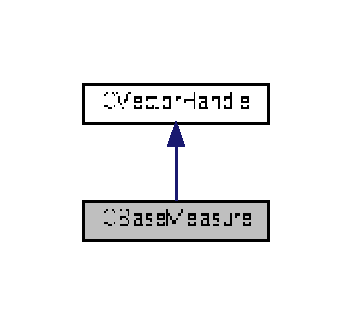
\includegraphics[width=169pt]{d6/d40/classCBaseMeasure__inherit__graph}
\end{center}
\end{figure}


Collaboration diagram for C\+Base\+Measure\+:
\nopagebreak
\begin{figure}[H]
\begin{center}
\leavevmode
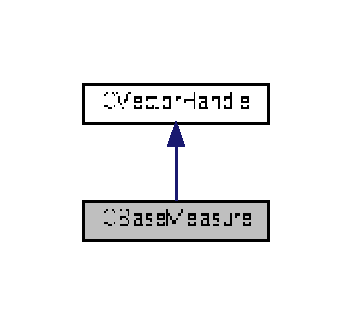
\includegraphics[width=169pt]{de/d06/classCBaseMeasure__coll__graph}
\end{center}
\end{figure}
\subsection*{Public Member Functions}
\begin{DoxyCompactItemize}
\item 
\hyperlink{classCBaseMeasure_a6a369b1e556d95a938b0e75647b5a602}{C\+Base\+Measure} ()
\begin{DoxyCompactList}\small\item\em default constructor\+: ~\newline
 initialize all member vectors \end{DoxyCompactList}\item 
\hyperlink{classCBaseMeasure_aca2735196a7e6e6524d73327d95d4a19}{$\sim$\+C\+Base\+Measure} ()
\begin{DoxyCompactList}\small\item\em destructor\+: clears all member vectors \end{DoxyCompactList}\item 
const double \hyperlink{classCBaseMeasure_abae752b654d90bcf0fa795cc9d4fb0ac}{Offset} (unsigned int Base\+Measure\+Enum)
\begin{DoxyCompactList}\small\item\em returns the offset for the converstion to the SI measure for the given \hyperlink{BaseMeasure_8h_ac90e5164ccf1f0d648fba7e94b229a11}{e\+Base\+Measure} \end{DoxyCompactList}\item 
\hyperlink{BaseMeasure_8h_ac90e5164ccf1f0d648fba7e94b229a11}{e\+Base\+Measure} \hyperlink{classCBaseMeasure_a4a2040454722a288e24babbacef30d01}{S\+I\+ID} (const \hyperlink{BaseMeasure_8h_ac90e5164ccf1f0d648fba7e94b229a11}{e\+Base\+Measure} Base\+Measure\+Enum)
\begin{DoxyCompactList}\small\item\em returns the \hyperlink{BaseMeasure_8h_ac90e5164ccf1f0d648fba7e94b229a11}{e\+Base\+Measure} of the SI measure for the given \hyperlink{BaseMeasure_8h_ac90e5164ccf1f0d648fba7e94b229a11}{e\+Base\+Measure} \end{DoxyCompactList}\item 
const string \hyperlink{classCBaseMeasure_acb998b7f15d9aa3530b2cb0b910177fd}{Debug\+Out} (const \hyperlink{BaseMeasure_8h_ac90e5164ccf1f0d648fba7e94b229a11}{e\+Base\+Measure} Base\+Measure\+Enum)
\begin{DoxyCompactList}\small\item\em output for debugging purpose for given index \end{DoxyCompactList}\item 
\hyperlink{BaseMeasure_8h_ac90e5164ccf1f0d648fba7e94b229a11}{e\+Base\+Measure} \hyperlink{classCBaseMeasure_a8476cf22a5fdcde4df0efc05cde70b45}{Get\+I\+D\+By\+Short\+Label} (const string \&str\+Short\+Label)
\begin{DoxyCompactList}\small\item\em returns the enum (index) of the base measure by searching the vstr\+Short-\/$>$. \end{DoxyCompactList}\item 
\hyperlink{BaseMeasure_8h_ac90e5164ccf1f0d648fba7e94b229a11}{e\+Base\+Measure} \hyperlink{classCBaseMeasure_a5c55d072ffe8e9b5fbe7713039987084}{Get\+I\+D\+By\+Long\+Label} (const string \&str\+Long\+Label)
\begin{DoxyCompactList}\small\item\em returns the enum (index) of the base measure by searching the vstr\+Long \end{DoxyCompactList}\end{DoxyCompactItemize}
\subsection*{Public Attributes}
\begin{DoxyCompactItemize}
\item 
vector$<$ int $>$ $\ast$ \hyperlink{classCBaseMeasure_aaaddf8a6ce321b282885953439472390}{vn\+S\+I\+Index}
\begin{DoxyCompactList}\small\item\em keeps the index of the corresponding SI unit\+: is its own unit in case it is the SI unit itself \end{DoxyCompactList}\item 
vector$<$ double $>$ $\ast$ \hyperlink{classCBaseMeasure_a7220e3dfd4fbdd319a5c3c6af844259e}{vd\+Offset}
\begin{DoxyCompactList}\small\item\em keeps the offset for the conversion to the SI Unit \end{DoxyCompactList}\end{DoxyCompactItemize}
\subsection*{Additional Inherited Members}


\subsection{Detailed Description}
\hyperlink{classCBaseMeasure}{C\+Base\+Measure}\+: represents the base-\/measure part of a measure.~\newline
 For example milli degree celsius consists of the base-\/measure part \char`\"{}degree celsius\char`\"{} (see \hyperlink{classCBaseMeasure}{C\+Base\+Measure}) and the pre-\/measure part \char`\"{}milli\char`\"{} (see \hyperlink{classCPreMeasure}{C\+Pre\+Measure}). ~\newline
 This class handles vectors of\+: 


\begin{DoxyItemize}
\item SI index (e.\+g. for \hyperlink{BaseMeasure_8h_ac90e5164ccf1f0d648fba7e94b229a11a42cee40c384c9bbda9aa488151b590b4}{bm\+Deg\+Celsius} the SI index is \hyperlink{BaseMeasure_8h_ac90e5164ccf1f0d648fba7e94b229a11a7d519faa41d1d34d9c378cfc61254074}{bm\+Deg\+Kelvin})
\item base-\/measure factor (e.\+g. for °F with index \hyperlink{BaseMeasure_8h_ac90e5164ccf1f0d648fba7e94b229a11add58e3d33a5d9459dbe3bf9d3f90777c}{bm\+Deg\+Fahrenheit} the factor for the conversion to the SI measure °K with index \hyperlink{BaseMeasure_8h_ac90e5164ccf1f0d648fba7e94b229a11a7d519faa41d1d34d9c378cfc61254074}{bm\+Deg\+Kelvin} is 5/9)
\item base-\/measure offset (e.\+g. for °C with index \hyperlink{BaseMeasure_8h_ac90e5164ccf1f0d648fba7e94b229a11a42cee40c384c9bbda9aa488151b590b4}{bm\+Deg\+Celsius} the offset for the conversion to the SI measure °K with index \hyperlink{BaseMeasure_8h_ac90e5164ccf1f0d648fba7e94b229a11a7d519faa41d1d34d9c378cfc61254074}{bm\+Deg\+Kelvin} is 273.\+15°K)
\item the short label (e.\+g. for Volt with the index \hyperlink{BaseMeasure_8h_ac90e5164ccf1f0d648fba7e94b229a11a662f2aa09627247b53e6f3c5cd10815e}{bm\+Volt} the short label is \char`\"{}\+V\char`\"{})
\item the long label (e.\+g. for Volt with the index \hyperlink{BaseMeasure_8h_ac90e5164ccf1f0d648fba7e94b229a11a662f2aa09627247b53e6f3c5cd10815e}{bm\+Volt} the short label is \char`\"{}volt\char`\"{})~\newline
 These vectors are accessed by the indices defined by the enum \hyperlink{BaseMeasure_8h_ac90e5164ccf1f0d648fba7e94b229a11}{e\+Base\+Measure}.~\newline
 
\end{DoxyItemize}

Definition at line 72 of file Base\+Measure.\+h.



\subsection{Constructor \& Destructor Documentation}
\mbox{\Hypertarget{classCBaseMeasure_a6a369b1e556d95a938b0e75647b5a602}\label{classCBaseMeasure_a6a369b1e556d95a938b0e75647b5a602}} 
\index{C\+Base\+Measure@{C\+Base\+Measure}!C\+Base\+Measure@{C\+Base\+Measure}}
\index{C\+Base\+Measure@{C\+Base\+Measure}!C\+Base\+Measure@{C\+Base\+Measure}}
\subsubsection{\texorpdfstring{C\+Base\+Measure()}{CBaseMeasure()}}
{\footnotesize\ttfamily C\+Base\+Measure\+::\+C\+Base\+Measure (\begin{DoxyParamCaption}{ }\end{DoxyParamCaption})}



default constructor\+: ~\newline
 initialize all member vectors 

initializes all relevant vectors describing a unit


\begin{DoxyItemize}
\item \hyperlink{classCVectorHandle_afb50c8a33d4cf70bf92c644dca409ea2}{C\+Base\+Measure\+::vstr\+Short}
\item \hyperlink{classCVectorHandle_a71bec0e385b9ca8e5ffa174b559da9f8}{C\+Base\+Measure\+::vstr\+Long}
\item \hyperlink{classCBaseMeasure_aaaddf8a6ce321b282885953439472390}{C\+Base\+Measure\+::vn\+S\+I\+Index}
\item \hyperlink{classCBaseMeasure_a7220e3dfd4fbdd319a5c3c6af844259e}{C\+Base\+Measure\+::vd\+Offset}
\item \hyperlink{classCVectorHandle_af8f8b2e0da8363e695872ca85f33364e}{C\+Base\+Measure\+::vd\+Factor} 
\end{DoxyItemize}

Definition at line 31 of file Base\+Measure.\+cpp.



References bm\+Ampere, bm\+Day, bm\+Deg\+Celsius, bm\+Deg\+Fahrenheit, bm\+Deg\+Kelvin, bm\+Farad, bm\+Foot, bm\+Hertz, bm\+Hour, bm\+Inch, bm\+Last, bm\+Meter, bm\+Mile, bm\+Minute, bm\+Number, bm\+Ohm, bm\+Second, bm\+Unknown, bm\+Volt, bm\+Yard, Omega, U\+N\+K\+N\+O\+W\+N\+\_\+\+I\+N\+D\+EX, U\+N\+K\+N\+O\+W\+N\+\_\+\+L\+O\+NG, U\+N\+K\+N\+O\+W\+N\+\_\+\+S\+H\+O\+RT, U\+N\+K\+N\+O\+W\+N\+\_\+\+V\+A\+L\+UE, C\+Vector\+Handle\+::vd\+Factor, vd\+Offset, vn\+S\+I\+Index, C\+Vector\+Handle\+::vstr\+Long, and C\+Vector\+Handle\+::vstr\+Short.

\mbox{\Hypertarget{classCBaseMeasure_aca2735196a7e6e6524d73327d95d4a19}\label{classCBaseMeasure_aca2735196a7e6e6524d73327d95d4a19}} 
\index{C\+Base\+Measure@{C\+Base\+Measure}!````~C\+Base\+Measure@{$\sim$\+C\+Base\+Measure}}
\index{````~C\+Base\+Measure@{$\sim$\+C\+Base\+Measure}!C\+Base\+Measure@{C\+Base\+Measure}}
\subsubsection{\texorpdfstring{$\sim$\+C\+Base\+Measure()}{~CBaseMeasure()}}
{\footnotesize\ttfamily C\+Base\+Measure\+::$\sim$\+C\+Base\+Measure (\begin{DoxyParamCaption}{ }\end{DoxyParamCaption})}



destructor\+: clears all member vectors 


\begin{DoxyItemize}
\item \hyperlink{classCVectorHandle_afb50c8a33d4cf70bf92c644dca409ea2}{C\+Base\+Measure\+::vstr\+Short}
\item \hyperlink{classCVectorHandle_a71bec0e385b9ca8e5ffa174b559da9f8}{C\+Base\+Measure\+::vstr\+Long}
\item \hyperlink{classCBaseMeasure_aaaddf8a6ce321b282885953439472390}{C\+Base\+Measure\+::vn\+S\+I\+Index}
\item \hyperlink{classCBaseMeasure_a7220e3dfd4fbdd319a5c3c6af844259e}{C\+Base\+Measure\+::vd\+Offset}
\item \hyperlink{classCVectorHandle_af8f8b2e0da8363e695872ca85f33364e}{C\+Base\+Measure\+::vd\+Factor} clears all member vectors 
\end{DoxyItemize}

Definition at line 159 of file Base\+Measure.\+cpp.



References vd\+Offset, and vn\+S\+I\+Index.



\subsection{Member Function Documentation}
\mbox{\Hypertarget{classCBaseMeasure_acb998b7f15d9aa3530b2cb0b910177fd}\label{classCBaseMeasure_acb998b7f15d9aa3530b2cb0b910177fd}} 
\index{C\+Base\+Measure@{C\+Base\+Measure}!Debug\+Out@{Debug\+Out}}
\index{Debug\+Out@{Debug\+Out}!C\+Base\+Measure@{C\+Base\+Measure}}
\subsubsection{\texorpdfstring{Debug\+Out()}{DebugOut()}}
{\footnotesize\ttfamily const string C\+Base\+Measure\+::\+Debug\+Out (\begin{DoxyParamCaption}\item[{const \hyperlink{BaseMeasure_8h_ac90e5164ccf1f0d648fba7e94b229a11}{e\+Base\+Measure}}]{Base\+Measure\+Enum }\end{DoxyParamCaption})}



output for debugging purpose for given index 


\begin{DoxyParams}{Parameters}
{\em Base\+Measure\+Enum} & index of base measure \\
\hline
\end{DoxyParams}
\begin{DoxyReturn}{Returns}
const string 
\end{DoxyReturn}


Definition at line 165 of file Base\+Measure.\+cpp.



References C\+Vector\+Handle\+::\+Factor(), C\+Vector\+Handle\+::\+Long(), Offset(), C\+Vector\+Handle\+::\+Short(), and S\+I\+I\+D().

\mbox{\Hypertarget{classCBaseMeasure_a5c55d072ffe8e9b5fbe7713039987084}\label{classCBaseMeasure_a5c55d072ffe8e9b5fbe7713039987084}} 
\index{C\+Base\+Measure@{C\+Base\+Measure}!Get\+I\+D\+By\+Long\+Label@{Get\+I\+D\+By\+Long\+Label}}
\index{Get\+I\+D\+By\+Long\+Label@{Get\+I\+D\+By\+Long\+Label}!C\+Base\+Measure@{C\+Base\+Measure}}
\subsubsection{\texorpdfstring{Get\+I\+D\+By\+Long\+Label()}{GetIDByLongLabel()}}
{\footnotesize\ttfamily \hyperlink{BaseMeasure_8h_ac90e5164ccf1f0d648fba7e94b229a11}{e\+Base\+Measure} C\+Base\+Measure\+::\+Get\+I\+D\+By\+Long\+Label (\begin{DoxyParamCaption}\item[{const string \&}]{str\+Long\+Label }\end{DoxyParamCaption})\hspace{0.3cm}{\ttfamily [inline]}}



returns the enum (index) of the base measure by searching the vstr\+Long 


\begin{DoxyParams}{Parameters}
{\em str\+Long\+Label} & \\
\hline
\end{DoxyParams}
\begin{DoxyReturn}{Returns}
e\+Base\+Measure 
\end{DoxyReturn}


Definition at line 150 of file Base\+Measure.\+h.



References C\+Vector\+Handle\+::\+Get\+Index\+By\+Long\+Label().

\mbox{\Hypertarget{classCBaseMeasure_a8476cf22a5fdcde4df0efc05cde70b45}\label{classCBaseMeasure_a8476cf22a5fdcde4df0efc05cde70b45}} 
\index{C\+Base\+Measure@{C\+Base\+Measure}!Get\+I\+D\+By\+Short\+Label@{Get\+I\+D\+By\+Short\+Label}}
\index{Get\+I\+D\+By\+Short\+Label@{Get\+I\+D\+By\+Short\+Label}!C\+Base\+Measure@{C\+Base\+Measure}}
\subsubsection{\texorpdfstring{Get\+I\+D\+By\+Short\+Label()}{GetIDByShortLabel()}}
{\footnotesize\ttfamily \hyperlink{BaseMeasure_8h_ac90e5164ccf1f0d648fba7e94b229a11}{e\+Base\+Measure} C\+Base\+Measure\+::\+Get\+I\+D\+By\+Short\+Label (\begin{DoxyParamCaption}\item[{const string \&}]{str\+Short\+Label }\end{DoxyParamCaption})\hspace{0.3cm}{\ttfamily [inline]}}



returns the enum (index) of the base measure by searching the vstr\+Short-\/$>$. 


\begin{DoxyParams}{Parameters}
{\em str\+Short\+Label} & short label of the base measure (e.\+g. \char`\"{}\+V\char`\"{} ) \\
\hline
\end{DoxyParams}
\begin{DoxyReturn}{Returns}
e\+Base\+Measure\+: the base-\/measure index (e.\+g. e\+Base\+Measure\+::bm\+Volt) 
\end{DoxyReturn}


Definition at line 139 of file Base\+Measure.\+h.



References C\+Vector\+Handle\+::\+Get\+Index\+By\+Short\+Label().

\mbox{\Hypertarget{classCBaseMeasure_abae752b654d90bcf0fa795cc9d4fb0ac}\label{classCBaseMeasure_abae752b654d90bcf0fa795cc9d4fb0ac}} 
\index{C\+Base\+Measure@{C\+Base\+Measure}!Offset@{Offset}}
\index{Offset@{Offset}!C\+Base\+Measure@{C\+Base\+Measure}}
\subsubsection{\texorpdfstring{Offset()}{Offset()}}
{\footnotesize\ttfamily const double C\+Base\+Measure\+::\+Offset (\begin{DoxyParamCaption}\item[{unsigned int}]{Base\+Measure\+Enum }\end{DoxyParamCaption})\hspace{0.3cm}{\ttfamily [inline]}}



returns the offset for the converstion to the SI measure for the given \hyperlink{BaseMeasure_8h_ac90e5164ccf1f0d648fba7e94b229a11}{e\+Base\+Measure} 


\begin{DoxyParams}{Parameters}
{\em Base\+Measure\+Enum} & index of the \\
\hline
\end{DoxyParams}
\begin{DoxyReturn}{Returns}
const double 
\end{DoxyReturn}


Definition at line 108 of file Base\+Measure.\+h.



References Get\+Element\+From\+Vector\+By\+Index().

\mbox{\Hypertarget{classCBaseMeasure_a4a2040454722a288e24babbacef30d01}\label{classCBaseMeasure_a4a2040454722a288e24babbacef30d01}} 
\index{C\+Base\+Measure@{C\+Base\+Measure}!S\+I\+ID@{S\+I\+ID}}
\index{S\+I\+ID@{S\+I\+ID}!C\+Base\+Measure@{C\+Base\+Measure}}
\subsubsection{\texorpdfstring{S\+I\+I\+D()}{SIID()}}
{\footnotesize\ttfamily \hyperlink{BaseMeasure_8h_ac90e5164ccf1f0d648fba7e94b229a11}{e\+Base\+Measure} C\+Base\+Measure\+::\+S\+I\+ID (\begin{DoxyParamCaption}\item[{const \hyperlink{BaseMeasure_8h_ac90e5164ccf1f0d648fba7e94b229a11}{e\+Base\+Measure}}]{Base\+Measure\+Enum }\end{DoxyParamCaption})\hspace{0.3cm}{\ttfamily [inline]}}



returns the \hyperlink{BaseMeasure_8h_ac90e5164ccf1f0d648fba7e94b229a11}{e\+Base\+Measure} of the SI measure for the given \hyperlink{BaseMeasure_8h_ac90e5164ccf1f0d648fba7e94b229a11}{e\+Base\+Measure} 


\begin{DoxyParams}{Parameters}
{\em Base\+Measure\+Enum} & p\+\_\+\+Base\+Measure\+Enum\+:... \\
\hline
\end{DoxyParams}
\begin{DoxyReturn}{Returns}
e\+Base\+Measure 
\end{DoxyReturn}


Definition at line 119 of file Base\+Measure.\+h.



References Get\+Element\+From\+Vector\+By\+Index().



\subsection{Member Data Documentation}
\mbox{\Hypertarget{classCBaseMeasure_a7220e3dfd4fbdd319a5c3c6af844259e}\label{classCBaseMeasure_a7220e3dfd4fbdd319a5c3c6af844259e}} 
\index{C\+Base\+Measure@{C\+Base\+Measure}!vd\+Offset@{vd\+Offset}}
\index{vd\+Offset@{vd\+Offset}!C\+Base\+Measure@{C\+Base\+Measure}}
\subsubsection{\texorpdfstring{vd\+Offset}{vdOffset}}
{\footnotesize\ttfamily vector$<$double$>$$\ast$ C\+Base\+Measure\+::vd\+Offset}



keeps the offset for the conversion to the SI Unit 



Definition at line 165 of file Base\+Measure.\+h.

\mbox{\Hypertarget{classCBaseMeasure_aaaddf8a6ce321b282885953439472390}\label{classCBaseMeasure_aaaddf8a6ce321b282885953439472390}} 
\index{C\+Base\+Measure@{C\+Base\+Measure}!vn\+S\+I\+Index@{vn\+S\+I\+Index}}
\index{vn\+S\+I\+Index@{vn\+S\+I\+Index}!C\+Base\+Measure@{C\+Base\+Measure}}
\subsubsection{\texorpdfstring{vn\+S\+I\+Index}{vnSIIndex}}
{\footnotesize\ttfamily vector$<$int$>$$\ast$ C\+Base\+Measure\+::vn\+S\+I\+Index}



keeps the index of the corresponding SI unit\+: is its own unit in case it is the SI unit itself 



Definition at line 159 of file Base\+Measure.\+h.



The documentation for this class was generated from the following files\+:\begin{DoxyCompactItemize}
\item 
Floating\+Measure/\+Measure/\hyperlink{BaseMeasure_8h}{Base\+Measure.\+h}\item 
Floating\+Measure/\+Measure/\hyperlink{BaseMeasure_8cpp}{Base\+Measure.\+cpp}\end{DoxyCompactItemize}

\hypertarget{classCComplexMeasure}{}\section{C\+Complex\+Measure Class Reference}
\label{classCComplexMeasure}\index{C\+Complex\+Measure@{C\+Complex\+Measure}}


\hyperlink{classCComplexMeasure}{C\+Complex\+Measure}\+: represents a list of measures (i.\+e. \hyperlink{classCSimpleMeasure}{C\+Simple\+Measure}) chained by operators $\ast$ and / ~\newline
 This class handles\+:  




{\ttfamily \#include $<$Complex\+Measure.\+h$>$}



Collaboration diagram for C\+Complex\+Measure\+:
\nopagebreak
\begin{figure}[H]
\begin{center}
\leavevmode
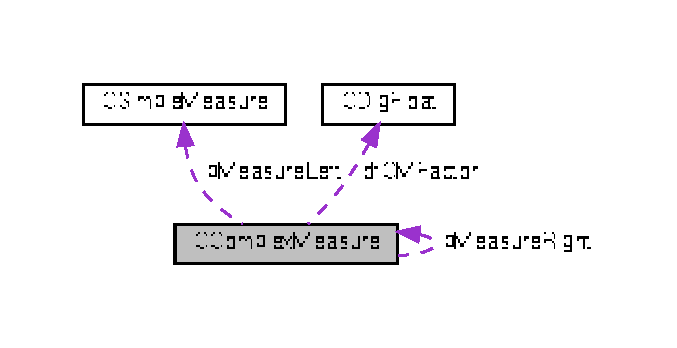
\includegraphics[width=325pt]{d6/d10/classCComplexMeasure__coll__graph}
\end{center}
\end{figure}
\subsection*{Public Member Functions}
\begin{DoxyCompactItemize}
\item 
\hyperlink{classCComplexMeasure_a5501594d4a8efdf565aa4c6bc6ce0379}{C\+Complex\+Measure} ()
\item 
\hyperlink{classCComplexMeasure_a50de70ddcb4b2b64c238d686e2f85419}{C\+Complex\+Measure} (const \hyperlink{classCComplexMeasure}{C\+Complex\+Measure} \&other)
\begin{DoxyCompactList}\small\item\em Copy constructor\+: calls \hyperlink{classCComplexMeasure}{C\+Complex\+Measure}\+:\+:~\newline
 calls \hyperlink{classCComplexMeasure_aed6efc43efe99d8cf1072ac98ec8d21c}{C\+Complex\+Measure\+::\+\_\+\+Init}, newly allocates \hyperlink{classCComplexMeasure_a4d68f86891a036df81f5b1a344c36f27}{C\+Complex\+Measure\+::p\+Measure\+Left} and \hyperlink{classCComplexMeasure_abbafc4b16676d223ed34860b8ece1b6b}{C\+Complex\+Measure\+::p\+Measure\+Right} from \char`\"{}other\char`\"{} \hyperlink{classCComplexMeasure}{C\+Complex\+Measure}. \end{DoxyCompactList}\item 
\hyperlink{classCComplexMeasure_a0a0946c508c95e4baf22a0bd5831c1b8}{C\+Complex\+Measure} (const \hyperlink{PreMeasure_8h_a6c81167b8d4c2badde42f81cb7214620}{e\+Pre\+Measure} Pre\+Measure\+Enum, const \hyperlink{BaseMeasure_8h_ac90e5164ccf1f0d648fba7e94b229a11}{e\+Base\+Measure} Base\+Measure\+Enum)
\begin{DoxyCompactList}\small\item\em Constructor by \hyperlink{PreMeasure_8h_a6c81167b8d4c2badde42f81cb7214620}{e\+Pre\+Measure} index and \hyperlink{BaseMeasure_8h_ac90e5164ccf1f0d648fba7e94b229a11}{e\+Base\+Measure} index\+:~\newline
 only sets \+::p\+Measure\+Left and deletes \+::p\+Measure\+Right. \end{DoxyCompactList}\item 
\hyperlink{classCComplexMeasure_a876e7030b4576f59ab66793ed3e7b50e}{C\+Complex\+Measure} (const \hyperlink{classCComplexMeasure}{C\+Complex\+Measure} $\ast$other)
\begin{DoxyCompactList}\small\item\em Copy constructor with pointer arg. \+: ~\newline
 calls \hyperlink{classCComplexMeasure_aed6efc43efe99d8cf1072ac98ec8d21c}{C\+Complex\+Measure\+::\+\_\+\+Init}, newly allocates \hyperlink{classCComplexMeasure_a4d68f86891a036df81f5b1a344c36f27}{C\+Complex\+Measure\+::p\+Measure\+Left} and \hyperlink{classCComplexMeasure_abbafc4b16676d223ed34860b8ece1b6b}{C\+Complex\+Measure\+::p\+Measure\+Right} from \char`\"{}other\char`\"{} \hyperlink{classCComplexMeasure}{C\+Complex\+Measure}. \end{DoxyCompactList}\item 
\hyperlink{classCComplexMeasure_a4b6895d4eef03df92d8ea1d8ad4f2f3d}{$\sim$\+C\+Complex\+Measure} ()
\item 
\hyperlink{classCComplexMeasure}{C\+Complex\+Measure} \& \hyperlink{classCComplexMeasure_a37668c1f7c157050080c0065ecbb596d}{operator=} (const \hyperlink{classCComplexMeasure}{C\+Complex\+Measure} \&other)
\begin{DoxyCompactList}\small\item\em assignment operator\+: \end{DoxyCompactList}\item 
\hyperlink{classCComplexMeasure}{C\+Complex\+Measure} \& \hyperlink{classCComplexMeasure_a66de753c892ed0a82fa8f2eb4d98029d}{operator$\ast$=} (const \hyperlink{classCComplexMeasure}{C\+Complex\+Measure} \&other)
\begin{DoxyCompactList}\small\item\em operator $\ast$=\+: calls \hyperlink{classCComplexMeasure_aee812c93b8b2fe3839e9a38df63cfd53}{C\+Complex\+Measure\+::\+\_\+\+Allocate\+Last\+Unset\+Measure\+Right} \end{DoxyCompactList}\item 
\hyperlink{classCComplexMeasure}{C\+Complex\+Measure} \& \hyperlink{classCComplexMeasure_a68c42a3ea08d1482f4dfdda5e34407f5}{operator/=} (const \hyperlink{classCComplexMeasure}{C\+Complex\+Measure} \&other)
\begin{DoxyCompactList}\small\item\em operator /=\+: calls \hyperlink{classCComplexMeasure_aee812c93b8b2fe3839e9a38df63cfd53}{C\+Complex\+Measure\+::\+\_\+\+Allocate\+Last\+Unset\+Measure\+Right} \end{DoxyCompactList}\item 
\hyperlink{classCComplexMeasure}{C\+Complex\+Measure} \hyperlink{classCComplexMeasure_afb04c59abf1f8ed44fe13d56df5d322c}{operator$\ast$} (const \hyperlink{classCComplexMeasure}{C\+Complex\+Measure} \&other)
\begin{DoxyCompactList}\small\item\em operator $\ast$\+: calls \hyperlink{classCComplexMeasure_a66de753c892ed0a82fa8f2eb4d98029d}{C\+Complex\+Measure\+::operator$\ast$=} with a copy of calling instance \end{DoxyCompactList}\item 
\hyperlink{classCComplexMeasure}{C\+Complex\+Measure} \hyperlink{classCComplexMeasure_a730c8745ab3d499a20d09f6faa47bdd2}{operator/} (const \hyperlink{classCComplexMeasure}{C\+Complex\+Measure} \&other)
\begin{DoxyCompactList}\small\item\em operator /\+: calls \hyperlink{classCComplexMeasure_a68c42a3ea08d1482f4dfdda5e34407f5}{C\+Complex\+Measure\+::operator/=} with a copy of calling instance \end{DoxyCompactList}\item 
bool \hyperlink{classCComplexMeasure_a30c168c8fbc0587835a11914f8af69e9}{operator==} (const \hyperlink{classCComplexMeasure}{C\+Complex\+Measure} \&other) const
\item 
bool \hyperlink{classCComplexMeasure_ab5e7581c34b128a8b24a7237094a4fe4}{operator!=} (const \hyperlink{classCComplexMeasure}{C\+Complex\+Measure} \&other) const
\item 
bool \hyperlink{classCComplexMeasure_aa807816cc8d410ff08e482c5e942a1a9}{Compatible} (const \hyperlink{classCComplexMeasure}{C\+Complex\+Measure} \&other) const
\begin{DoxyCompactList}\small\item\em checks for a \hyperlink{classCComplexMeasure}{C\+Complex\+Measure} being scaled (i.\+e. f$\ast$ this) to this \end{DoxyCompactList}\item 
void \hyperlink{classCComplexMeasure_a999dd5e5bb71a6bc548f959879b4e12f}{Scale\+To} (const \hyperlink{classCComplexMeasure}{C\+Complex\+Measure} \&other)
\begin{DoxyCompactList}\small\item\em scale to other compatible \hyperlink{classCComplexMeasure}{C\+Complex\+Measure} \end{DoxyCompactList}\item 
void \hyperlink{classCComplexMeasure_a47dca89bc28bbb257f81df4d363be623}{Set\+By\+ID} (const \hyperlink{PreMeasure_8h_a6c81167b8d4c2badde42f81cb7214620}{e\+Pre\+Measure} Pre\+Measure\+Enum, const \hyperlink{BaseMeasure_8h_ac90e5164ccf1f0d648fba7e94b229a11}{e\+Base\+Measure} Base\+Measure\+Enum)
\begin{DoxyCompactList}\small\item\em sets the p\+Measure\+Left calling \hyperlink{classCSimpleMeasure_a6945aa333dca5623482d38cd9a7e3225}{C\+Simple\+Measure\+::\+Set\+By\+ID} \end{DoxyCompactList}\item 
void \hyperlink{classCComplexMeasure_a87cc1f3c3f0dafd7cbe00634124c8d46}{Normalize} ()
\begin{DoxyCompactList}\small\item\em sets all measures to SI and calculates S\+Ipremeasure and d\+S\+I\+Factor\+: calls internal function C\+Complex\+Measure\+::\+\_\+\+Normalize(nullptr,nullptr) \end{DoxyCompactList}\item 
const \hyperlink{classCDigFloat}{C\+Dig\+Float} \& \hyperlink{classCComplexMeasure_acdcab22efa233ea1c0e607bf22028afd}{C\+M\+Factor} ()
\begin{DoxyCompactList}\small\item\em getter for df\+C\+M\+Factor \end{DoxyCompactList}\item 
const int \hyperlink{classCComplexMeasure_a06355541d6d9b843b9d68156a0297f51}{C\+M\+Exp10} ()
\begin{DoxyCompactList}\small\item\em getter for n\+C\+M\+Exp10 \end{DoxyCompactList}\item 
void \hyperlink{classCComplexMeasure_addb4e69033f2c32fb3bf4a3aef5e1470}{Simplify} ()
\begin{DoxyCompactList}\small\item\em simplifies complex measure (e.\+g. uV / mV $\ast$ A = A (exp10 += -\/3)) the factors of the premeasures are collected in the C\+Complex\+Measure\+::n\+Exp10 member of this class \end{DoxyCompactList}\item 
bool \hyperlink{classCComplexMeasure_a1b777eef864d0c7a959dbeee321e881d}{Valid} ()
\begin{DoxyCompactList}\small\item\em check for valid measures\+: if one invalid measure is found --$>$ everything is invalid \end{DoxyCompactList}\item 
string \hyperlink{classCComplexMeasure_ab6a38e7259d7c27e735ff12fd711c5d5}{O\+P\+Short} ()
\begin{DoxyCompactList}\small\item\em prints the short label of the \hyperlink{classCComplexMeasure_ae22369976a7e5570add11a4172dcf062}{C\+Complex\+Measure\+::op\+Enum} \end{DoxyCompactList}\item 
string \hyperlink{classCComplexMeasure_aefe6745e32e203d0dd2b7a4e13504142}{Print\+All\+Short} ()
\begin{DoxyCompactList}\small\item\em prints the premeasure and the base measure short labels \end{DoxyCompactList}\item 
string \hyperlink{classCComplexMeasure_a83c00029eaad1c0c59fd1210108981dc}{Debug\+Out} ()
\begin{DoxyCompactList}\small\item\em prints all members\+: can be applied for debugging purpose \end{DoxyCompactList}\end{DoxyCompactItemize}
\subsection*{Protected Member Functions}
\begin{DoxyCompactItemize}
\item 
void \hyperlink{classCComplexMeasure_aed6efc43efe99d8cf1072ac98ec8d21c}{\+\_\+\+Init} (bool b\+Allocate\+Measure\+Left=true)
\item 
void \hyperlink{classCComplexMeasure_a6f071c1bd1340fea78a2aa90d1b6496f}{\+\_\+\+Invert\+OP} ()
\item 
void \hyperlink{classCComplexMeasure_aee812c93b8b2fe3839e9a38df63cfd53}{\+\_\+\+Allocate\+Last\+Unset\+Measure\+Right} (\hyperlink{classCComplexMeasure}{C\+Complex\+Measure} \&cm\+Operand\+Left, const \hyperlink{classCComplexMeasure}{C\+Complex\+Measure} \&cm\+Operand\+Right, const \hyperlink{MeasureOperator_8h_a1431c79e3ad4b4c5bcc9f31f188538f2}{e\+Operation} Operation\+Enum)
\begin{DoxyCompactList}\small\item\em helping function allocating the last p\+Measure\+Right, joining with given operation \end{DoxyCompactList}\item 
void \hyperlink{classCComplexMeasure_abd62182294ebd217cdd9af40d0af7e38}{\+\_\+\+Normalize} (\hyperlink{MeasureOperator_8h_a1431c79e3ad4b4c5bcc9f31f188538f2}{e\+Operation} $\ast$\&p\+Previous\+OP, int $\ast$\&pd\+Temp\+Pre\+Measure\+Exp10\+Collector, \hyperlink{classCDigFloat}{C\+Dig\+Float} $\ast$\&pd\+Temp\+C\+M\+Factor\+Collector, \hyperlink{classCComplexMeasure}{C\+Complex\+Measure} $\ast$\&p\+First\+Complex\+Measure)
\begin{DoxyCompactList}\small\item\em internally called function\+: called by \hyperlink{classCComplexMeasure_a87cc1f3c3f0dafd7cbe00634124c8d46}{C\+Complex\+Measure\+::\+Normalize} which sets all measures to SI and calculates S\+Ipremeasure and d\+S\+I\+Factor \end{DoxyCompactList}\item 
void \hyperlink{classCComplexMeasure_ad96c02d0791585e8bc138212e44bb743}{\+\_\+\+C\+Ollect\+C\+M\+Exp10\+C\+M\+Factor\+Wrapper} ()
\begin{DoxyCompactList}\small\item\em this function must always called when two C\+Complex\+Measures are joined (e.\+g. from function \+\_\+\+Allocate\+Last\+Unset\+Measure\+Right) \end{DoxyCompactList}\item 
void \hyperlink{classCComplexMeasure_aa87ac8d42bbb244fc77dae299ae35ca7}{\+\_\+\+C\+Ollect\+C\+M\+Exp10\+C\+M\+Factor} (\hyperlink{MeasureOperator_8h_a1431c79e3ad4b4c5bcc9f31f188538f2}{e\+Operation} $\ast$\&p\+Previous\+OP, int $\ast$\&pd\+Temp\+Pre\+Measure\+Exp10\+Collector, \hyperlink{classCDigFloat}{C\+Dig\+Float} $\ast$\&pd\+Temp\+C\+M\+Factor\+Collector, \hyperlink{classCComplexMeasure}{C\+Complex\+Measure} $\ast$\&p\+First\+Complex\+Measure)
\begin{DoxyCompactList}\small\item\em internal function called by every function which extents \hyperlink{classCComplexMeasure}{C\+Complex\+Measure} with \char`\"{}other\char`\"{} \hyperlink{classCComplexMeasure}{C\+Complex\+Measure} collects the C\+M\+Exp10 and C\+M\+Factor from \char`\"{}other\char`\"{} and unites it into the primary C\+M\+Factor and C\+M\+Exp10 \end{DoxyCompactList}\item 
void \hyperlink{classCComplexMeasure_ad2602b97f17c475a91454bf6bd1be1a4}{\+\_\+\+Collect\+Left\+Sort\+By\+Op} (map$<$ \hyperlink{MeasureOperator_8h_a1431c79e3ad4b4c5bcc9f31f188538f2}{e\+Operation}, \hyperlink{classCComplexMeasure}{C\+Complex\+Measure} $\ast$$>$ \&m\+Op\+Meas)
\begin{DoxyCompactList}\small\item\em collects p\+Measure\+Left with operands into m\+Op\+Meas --$>$ used for \hyperlink{classCComplexMeasure_addb4e69033f2c32fb3bf4a3aef5e1470}{C\+Complex\+Measure\+::\+Simplify} \end{DoxyCompactList}\item 
void \hyperlink{classCComplexMeasure_ac9bdfda3d2175532ba7e1f425e6b23b1}{\+\_\+\+Search\+And\+Shorten\+Same\+S\+I\+Index} (\hyperlink{classCComplexMeasure}{C\+Complex\+Measure} $\ast$p\+Shorten\+Partner, \hyperlink{MeasureOperator_8h_a1431c79e3ad4b4c5bcc9f31f188538f2}{e\+Operation} \&e\+O\+Pof\+Shorten\+Partner, \hyperlink{MeasureOperator_8h_a1431c79e3ad4b4c5bcc9f31f188538f2}{e\+Operation} \&e\+O\+Pof\+Consecutive\+Shorten\+Partner)
\begin{DoxyCompactList}\small\item\em searches \hyperlink{classCSimpleMeasure}{C\+Simple\+Measure} of consecutive p\+Measure\+Right, which p\+Measure\+Left have thesame SI index as p\+Measure\+Left of p\+Shorten\+Partner\+: stops if the first item is found, \hyperlink{classCComplexMeasure_a8f642a3a0044d4dc0492774bca8666e9}{C\+Complex\+Measure\+::\+\_\+\+Resolve\+Measure\+Left} for p\+Shorten\+Partner and the found item is called. This function is called as one step \hyperlink{classCComplexMeasure_addb4e69033f2c32fb3bf4a3aef5e1470}{C\+Complex\+Measure\+::\+Simplify} \end{DoxyCompactList}\item 
void \hyperlink{classCComplexMeasure_a8f642a3a0044d4dc0492774bca8666e9}{\+\_\+\+Resolve\+Measure\+Left} ()
\begin{DoxyCompactList}\small\item\em collects premeasure factor in n\+Exp10 and sets p\+Measure\+Left to (pm\+Ident, bm\+Number) \end{DoxyCompactList}\item 
void \hyperlink{classCComplexMeasure_a9eb89170847ab2ef592eace6453cf300}{\+\_\+\+Remove\+Neutral\+Numbers} (\hyperlink{classCComplexMeasure}{C\+Complex\+Measure} \&Previous\+Complex\+Measure)
\item 
void \hyperlink{classCComplexMeasure_ae66b48f40cc04866424ca5b7114d4adb}{\+\_\+\+Simplify} (\hyperlink{MeasureOperator_8h_a1431c79e3ad4b4c5bcc9f31f188538f2}{e\+Operation} \&Previous\+OP)
\item 
void \hyperlink{classCComplexMeasure_ae3605c75d2c571b06108b4b19af6618b}{\+\_\+\+Valid} (bool \&b\+Valid)
\begin{DoxyCompactList}\small\item\em recursive call of checking the p\+Measure\+Left measures being valid \end{DoxyCompactList}\item 
const double \hyperlink{classCComplexMeasure_a2c4086ab6b664259b820f554f647cdbd}{Release\+Exp10\+And\+Factor} ()
\begin{DoxyCompactList}\small\item\em returns the product of df\+C\+M\+Factor and pow(10,\+Exp10()) and resets factor to 1 and n\+Exp10 to 0 \end{DoxyCompactList}\item 
void \hyperlink{classCComplexMeasure_aaa6f3cf75ee0dd2a880adaaf43e81168}{C\+M\+Exp10} (const int Other\+Exp10)
\begin{DoxyCompactList}\small\item\em protected setter of n\+C\+M\+Exp10 ... for internal use only \end{DoxyCompactList}\item 
void \hyperlink{classCComplexMeasure_abc97b2ed29224bb00a912a94933192a2}{C\+M\+Factor} (const double Factor)
\begin{DoxyCompactList}\small\item\em protected setter of df\+C\+M\+Factor ... for internal use only \end{DoxyCompactList}\end{DoxyCompactItemize}
\subsection*{Protected Attributes}
\begin{DoxyCompactItemize}
\item 
\hyperlink{MeasureOperator_8h_a1431c79e3ad4b4c5bcc9f31f188538f2}{e\+Operation} \hyperlink{classCComplexMeasure_ae22369976a7e5570add11a4172dcf062}{op\+Enum}
\begin{DoxyCompactList}\small\item\em index of the corresponding operator of p\+Measure\+Left and p\+Measure\+Right \end{DoxyCompactList}\item 
\hyperlink{classCComplexMeasure}{C\+Complex\+Measure} $\ast$ \hyperlink{classCComplexMeasure_abbafc4b16676d223ed34860b8ece1b6b}{p\+Measure\+Right}
\begin{DoxyCompactList}\small\item\em right operand as complex measure (pointing to next p\+Measure\+Left, operator, and p\+Measure\+Right for a daisy chained list of complex measures \end{DoxyCompactList}\item 
\hyperlink{classCSimpleMeasure}{C\+Simple\+Measure} $\ast$ \hyperlink{classCComplexMeasure_a4d68f86891a036df81f5b1a344c36f27}{p\+Measure\+Left}
\begin{DoxyCompactList}\small\item\em left operand is a Simple\+Measure representant \end{DoxyCompactList}\item 
int \hyperlink{classCComplexMeasure_a52cfbd26747c0497cfe97c56f2ff38ea}{n\+C\+M\+Exp10}
\begin{DoxyCompactList}\small\item\em the epx10 which will be set e.\+g. for normalization or simplification collecting all Exp10 of Pre\+Measure\+Enum(see \hyperlink{classCComplexMeasure_addb4e69033f2c32fb3bf4a3aef5e1470}{C\+Complex\+Measure\+::\+Simplify()} and \hyperlink{classCComplexMeasure_a87cc1f3c3f0dafd7cbe00634124c8d46}{C\+Complex\+Measure\+::\+Normalize()}.) \end{DoxyCompactList}\item 
\hyperlink{classCDigFloat}{C\+Dig\+Float} \hyperlink{classCComplexMeasure_a21eecd9fd837fb73da2e6994b6c3fefe}{df\+C\+M\+Factor}
\begin{DoxyCompactList}\small\item\em the factor value which will be set e.\+g. for normalization or simplification collecting all SI factors(see \hyperlink{classCComplexMeasure_addb4e69033f2c32fb3bf4a3aef5e1470}{C\+Complex\+Measure\+::\+Simplify()} and \hyperlink{classCComplexMeasure_a87cc1f3c3f0dafd7cbe00634124c8d46}{C\+Complex\+Measure\+::\+Normalize()}.) \end{DoxyCompactList}\end{DoxyCompactItemize}
\subsection*{Friends}
\begin{DoxyCompactItemize}
\item 
class \hyperlink{classCComplexMeasure_a7e23751869edf87edc0feeb80eda78d9}{C\+Floating\+Measure}
\item 
class \hyperlink{classCComplexMeasure_ac06bbec937fbb103ef6191c80bfa5880}{C\+Simple\+Measure}
\end{DoxyCompactItemize}


\subsection{Detailed Description}
\hyperlink{classCComplexMeasure}{C\+Complex\+Measure}\+: represents a list of measures (i.\+e. \hyperlink{classCSimpleMeasure}{C\+Simple\+Measure}) chained by operators $\ast$ and / ~\newline
 This class handles\+: 


\begin{DoxyItemize}
\item operators and constructors for construction of complex measures (e.\+g. mV / kA )
\item simplification (e.\+g. V $\ast$ A / V --$>$ A)
\item normalization (e.\+g. mV $\rightarrow$ V)
\item comparison (e.\+g. mV / mA is equal to kV / kA)
\item compatibility check ( e.\+g. mV /kA is compatible with kA / mV)~\newline

\end{DoxyItemize}

R\+E\+M\+A\+RK\+: physical laws like the Ohm law is N\+OT (yet) meant to (and may be never will) ~\newline
 be considered within this class (i.\+e. ohm = volt / ampere ) 

Definition at line 49 of file Complex\+Measure.\+h.



\subsection{Constructor \& Destructor Documentation}
\mbox{\Hypertarget{classCComplexMeasure_a5501594d4a8efdf565aa4c6bc6ce0379}\label{classCComplexMeasure_a5501594d4a8efdf565aa4c6bc6ce0379}} 
\index{C\+Complex\+Measure@{C\+Complex\+Measure}!C\+Complex\+Measure@{C\+Complex\+Measure}}
\index{C\+Complex\+Measure@{C\+Complex\+Measure}!C\+Complex\+Measure@{C\+Complex\+Measure}}
\subsubsection{\texorpdfstring{C\+Complex\+Measure()}{CComplexMeasure()}\hspace{0.1cm}{\footnotesize\ttfamily [1/4]}}
{\footnotesize\ttfamily C\+Complex\+Measure\+::\+C\+Complex\+Measure (\begin{DoxyParamCaption}{ }\end{DoxyParamCaption})}

Default constructor\+: calls \hyperlink{classCComplexMeasure_aed6efc43efe99d8cf1072ac98ec8d21c}{C\+Complex\+Measure\+::\+\_\+\+Init()} 

Definition at line 27 of file Complex\+Measure.\+cpp.



References \+\_\+\+Init().

\mbox{\Hypertarget{classCComplexMeasure_a50de70ddcb4b2b64c238d686e2f85419}\label{classCComplexMeasure_a50de70ddcb4b2b64c238d686e2f85419}} 
\index{C\+Complex\+Measure@{C\+Complex\+Measure}!C\+Complex\+Measure@{C\+Complex\+Measure}}
\index{C\+Complex\+Measure@{C\+Complex\+Measure}!C\+Complex\+Measure@{C\+Complex\+Measure}}
\subsubsection{\texorpdfstring{C\+Complex\+Measure()}{CComplexMeasure()}\hspace{0.1cm}{\footnotesize\ttfamily [2/4]}}
{\footnotesize\ttfamily C\+Complex\+Measure\+::\+C\+Complex\+Measure (\begin{DoxyParamCaption}\item[{const \hyperlink{classCComplexMeasure}{C\+Complex\+Measure} \&}]{other }\end{DoxyParamCaption})}



Copy constructor\+: calls \hyperlink{classCComplexMeasure}{C\+Complex\+Measure}\+:\+:~\newline
 calls \hyperlink{classCComplexMeasure_aed6efc43efe99d8cf1072ac98ec8d21c}{C\+Complex\+Measure\+::\+\_\+\+Init}, newly allocates \hyperlink{classCComplexMeasure_a4d68f86891a036df81f5b1a344c36f27}{C\+Complex\+Measure\+::p\+Measure\+Left} and \hyperlink{classCComplexMeasure_abbafc4b16676d223ed34860b8ece1b6b}{C\+Complex\+Measure\+::p\+Measure\+Right} from \char`\"{}other\char`\"{} \hyperlink{classCComplexMeasure}{C\+Complex\+Measure}. 

Copy constructor\+: ~\newline
 calls \hyperlink{classCComplexMeasure_aed6efc43efe99d8cf1072ac98ec8d21c}{C\+Complex\+Measure\+::\+\_\+\+Init}, newly allocates \hyperlink{classCComplexMeasure_a4d68f86891a036df81f5b1a344c36f27}{C\+Complex\+Measure\+::p\+Measure\+Left} and \hyperlink{classCComplexMeasure_abbafc4b16676d223ed34860b8ece1b6b}{C\+Complex\+Measure\+::p\+Measure\+Right} from \char`\"{}other\char`\"{} \hyperlink{classCComplexMeasure}{C\+Complex\+Measure}


\begin{DoxyParams}{Parameters}
{\em other} & \hyperlink{classCComplexMeasure}{C\+Complex\+Measure} to \\
\hline
{\em other} & \hyperlink{classCComplexMeasure}{C\+Complex\+Measure}\& to copy from \\
\hline
\end{DoxyParams}


Definition at line 32 of file Complex\+Measure.\+cpp.



References \+\_\+\+Init(), C\+Complex\+Measure(), C\+Simple\+Measure, df\+C\+M\+Factor, n\+C\+M\+Exp10, op\+Enum, p\+Measure\+Left, and p\+Measure\+Right.

\mbox{\Hypertarget{classCComplexMeasure_a0a0946c508c95e4baf22a0bd5831c1b8}\label{classCComplexMeasure_a0a0946c508c95e4baf22a0bd5831c1b8}} 
\index{C\+Complex\+Measure@{C\+Complex\+Measure}!C\+Complex\+Measure@{C\+Complex\+Measure}}
\index{C\+Complex\+Measure@{C\+Complex\+Measure}!C\+Complex\+Measure@{C\+Complex\+Measure}}
\subsubsection{\texorpdfstring{C\+Complex\+Measure()}{CComplexMeasure()}\hspace{0.1cm}{\footnotesize\ttfamily [3/4]}}
{\footnotesize\ttfamily C\+Complex\+Measure\+::\+C\+Complex\+Measure (\begin{DoxyParamCaption}\item[{const \hyperlink{PreMeasure_8h_a6c81167b8d4c2badde42f81cb7214620}{e\+Pre\+Measure}}]{Pre\+Measure\+Enum,  }\item[{const \hyperlink{BaseMeasure_8h_ac90e5164ccf1f0d648fba7e94b229a11}{e\+Base\+Measure}}]{Base\+Measure\+Enum }\end{DoxyParamCaption})}



Constructor by \hyperlink{PreMeasure_8h_a6c81167b8d4c2badde42f81cb7214620}{e\+Pre\+Measure} index and \hyperlink{BaseMeasure_8h_ac90e5164ccf1f0d648fba7e94b229a11}{e\+Base\+Measure} index\+:~\newline
 only sets \+::p\+Measure\+Left and deletes \+::p\+Measure\+Right. 


\begin{DoxyParams}{Parameters}
{\em Pre\+Measure\+Enum} & pre-\/measure index \\
\hline
{\em Base\+Measure\+Enum} & base-\/measure index \\
\hline
\end{DoxyParams}


Definition at line 66 of file Complex\+Measure.\+cpp.



References \+\_\+\+Init(), p\+Measure\+Left, and C\+Simple\+Measure\+::\+Set\+By\+I\+D().

\mbox{\Hypertarget{classCComplexMeasure_a876e7030b4576f59ab66793ed3e7b50e}\label{classCComplexMeasure_a876e7030b4576f59ab66793ed3e7b50e}} 
\index{C\+Complex\+Measure@{C\+Complex\+Measure}!C\+Complex\+Measure@{C\+Complex\+Measure}}
\index{C\+Complex\+Measure@{C\+Complex\+Measure}!C\+Complex\+Measure@{C\+Complex\+Measure}}
\subsubsection{\texorpdfstring{C\+Complex\+Measure()}{CComplexMeasure()}\hspace{0.1cm}{\footnotesize\ttfamily [4/4]}}
{\footnotesize\ttfamily C\+Complex\+Measure\+::\+C\+Complex\+Measure (\begin{DoxyParamCaption}\item[{const \hyperlink{classCComplexMeasure}{C\+Complex\+Measure} $\ast$}]{other }\end{DoxyParamCaption})}



Copy constructor with pointer arg. \+: ~\newline
 calls \hyperlink{classCComplexMeasure_aed6efc43efe99d8cf1072ac98ec8d21c}{C\+Complex\+Measure\+::\+\_\+\+Init}, newly allocates \hyperlink{classCComplexMeasure_a4d68f86891a036df81f5b1a344c36f27}{C\+Complex\+Measure\+::p\+Measure\+Left} and \hyperlink{classCComplexMeasure_abbafc4b16676d223ed34860b8ece1b6b}{C\+Complex\+Measure\+::p\+Measure\+Right} from \char`\"{}other\char`\"{} \hyperlink{classCComplexMeasure}{C\+Complex\+Measure}. 


\begin{DoxyParams}{Parameters}
{\em other} & p\+\_\+other\+:... \\
\hline
\end{DoxyParams}


Definition at line 50 of file Complex\+Measure.\+cpp.



References \+\_\+\+Init(), C\+Complex\+Measure(), C\+Simple\+Measure, df\+C\+M\+Factor, n\+C\+M\+Exp10, op\+Enum, p\+Measure\+Left, and p\+Measure\+Right.

\mbox{\Hypertarget{classCComplexMeasure_a4b6895d4eef03df92d8ea1d8ad4f2f3d}\label{classCComplexMeasure_a4b6895d4eef03df92d8ea1d8ad4f2f3d}} 
\index{C\+Complex\+Measure@{C\+Complex\+Measure}!````~C\+Complex\+Measure@{$\sim$\+C\+Complex\+Measure}}
\index{````~C\+Complex\+Measure@{$\sim$\+C\+Complex\+Measure}!C\+Complex\+Measure@{C\+Complex\+Measure}}
\subsubsection{\texorpdfstring{$\sim$\+C\+Complex\+Measure()}{~CComplexMeasure()}}
{\footnotesize\ttfamily C\+Complex\+Measure\+::$\sim$\+C\+Complex\+Measure (\begin{DoxyParamCaption}{ }\end{DoxyParamCaption})}

Destructor 

Definition at line 72 of file Complex\+Measure.\+cpp.



References op\+Enum, op\+Unknown, p\+Measure\+Left, p\+Measure\+Right, $\sim$\+C\+Complex\+Measure(), and C\+Simple\+Measure\+::$\sim$\+C\+Simple\+Measure().



\subsection{Member Function Documentation}
\mbox{\Hypertarget{classCComplexMeasure_aee812c93b8b2fe3839e9a38df63cfd53}\label{classCComplexMeasure_aee812c93b8b2fe3839e9a38df63cfd53}} 
\index{C\+Complex\+Measure@{C\+Complex\+Measure}!\+\_\+\+Allocate\+Last\+Unset\+Measure\+Right@{\+\_\+\+Allocate\+Last\+Unset\+Measure\+Right}}
\index{\+\_\+\+Allocate\+Last\+Unset\+Measure\+Right@{\+\_\+\+Allocate\+Last\+Unset\+Measure\+Right}!C\+Complex\+Measure@{C\+Complex\+Measure}}
\subsubsection{\texorpdfstring{\+\_\+\+Allocate\+Last\+Unset\+Measure\+Right()}{\_AllocateLastUnsetMeasureRight()}}
{\footnotesize\ttfamily void C\+Complex\+Measure\+::\+\_\+\+Allocate\+Last\+Unset\+Measure\+Right (\begin{DoxyParamCaption}\item[{\hyperlink{classCComplexMeasure}{C\+Complex\+Measure} \&}]{cm\+Operand\+Left,  }\item[{const \hyperlink{classCComplexMeasure}{C\+Complex\+Measure} \&}]{cm\+Operand\+Right,  }\item[{const \hyperlink{MeasureOperator_8h_a1431c79e3ad4b4c5bcc9f31f188538f2}{e\+Operation}}]{Operation\+Enum }\end{DoxyParamCaption})\hspace{0.3cm}{\ttfamily [protected]}}



helping function allocating the last p\+Measure\+Right, joining with given operation 


\begin{DoxyParams}{Parameters}
{\em cm\+Operand\+Left} & \hyperlink{classCComplexMeasure}{C\+Complex\+Measure} left operand \\
\hline
{\em cm\+Operand\+Right} & \hyperlink{classCComplexMeasure}{C\+Complex\+Measure} right operand \\
\hline
{\em Operation\+Enum} & e\+Operation operation \\
\hline
\end{DoxyParams}


Definition at line 186 of file Complex\+Measure.\+cpp.



References \+\_\+\+C\+Ollect\+C\+M\+Exp10\+C\+M\+Factor\+Wrapper(), \+\_\+\+Invert\+O\+P(), C\+Complex\+Measure(), op\+Divide, op\+Enum, and p\+Measure\+Right.

\mbox{\Hypertarget{classCComplexMeasure_aa87ac8d42bbb244fc77dae299ae35ca7}\label{classCComplexMeasure_aa87ac8d42bbb244fc77dae299ae35ca7}} 
\index{C\+Complex\+Measure@{C\+Complex\+Measure}!\+\_\+\+C\+Ollect\+C\+M\+Exp10\+C\+M\+Factor@{\+\_\+\+C\+Ollect\+C\+M\+Exp10\+C\+M\+Factor}}
\index{\+\_\+\+C\+Ollect\+C\+M\+Exp10\+C\+M\+Factor@{\+\_\+\+C\+Ollect\+C\+M\+Exp10\+C\+M\+Factor}!C\+Complex\+Measure@{C\+Complex\+Measure}}
\subsubsection{\texorpdfstring{\+\_\+\+C\+Ollect\+C\+M\+Exp10\+C\+M\+Factor()}{\_COllectCMExp10CMFactor()}}
{\footnotesize\ttfamily void C\+Complex\+Measure\+::\+\_\+\+C\+Ollect\+C\+M\+Exp10\+C\+M\+Factor (\begin{DoxyParamCaption}\item[{\hyperlink{MeasureOperator_8h_a1431c79e3ad4b4c5bcc9f31f188538f2}{e\+Operation} $\ast$\&}]{p\+Previous\+OP,  }\item[{int $\ast$\&}]{pd\+Temp\+Pre\+Measure\+Exp10\+Collector,  }\item[{\hyperlink{classCDigFloat}{C\+Dig\+Float} $\ast$\&}]{pd\+Temp\+C\+M\+Factor\+Collector,  }\item[{\hyperlink{classCComplexMeasure}{C\+Complex\+Measure} $\ast$\&}]{p\+First\+Complex\+Measure }\end{DoxyParamCaption})\hspace{0.3cm}{\ttfamily [protected]}}



internal function called by every function which extents \hyperlink{classCComplexMeasure}{C\+Complex\+Measure} with \char`\"{}other\char`\"{} \hyperlink{classCComplexMeasure}{C\+Complex\+Measure} collects the C\+M\+Exp10 and C\+M\+Factor from \char`\"{}other\char`\"{} and unites it into the primary C\+M\+Factor and C\+M\+Exp10 


\begin{DoxyParams}{Parameters}
{\em p\+Previous\+OP} & e\+Operation operation of previous \hyperlink{classCComplexMeasure}{C\+Complex\+Measure} \\
\hline
{\em pd\+Temp\+Pre\+Measure\+Exp10\+Collector} & int pointer collecting all exp10 \\
\hline
{\em pd\+Temp\+C\+M\+Factor\+Collector} & \hyperlink{classCDigFloat}{C\+Dig\+Float} pointer collecting all \hyperlink{classCComplexMeasure_acdcab22efa233ea1c0e607bf22028afd}{C\+Complex\+Measure\+::\+C\+M\+Factor} \\
\hline
{\em p\+First\+Complex\+Measure} & \hyperlink{classCComplexMeasure}{C\+Complex\+Measure} first complex measure where collected exp10 and C\+M\+Factor are stored \\
\hline
\end{DoxyParams}


Definition at line 386 of file Complex\+Measure.\+cpp.



References \+\_\+\+C\+Ollect\+C\+M\+Exp10\+C\+M\+Factor(), C\+M\+Exp10(), C\+M\+Factor(), df\+C\+M\+Factor, op\+Divide, op\+Enum, op\+Mult, p\+Measure\+Right, Secure\+Delete\+Object\+Pointer(), and Secure\+Delete\+Vector\+Pointer().

\mbox{\Hypertarget{classCComplexMeasure_ad96c02d0791585e8bc138212e44bb743}\label{classCComplexMeasure_ad96c02d0791585e8bc138212e44bb743}} 
\index{C\+Complex\+Measure@{C\+Complex\+Measure}!\+\_\+\+C\+Ollect\+C\+M\+Exp10\+C\+M\+Factor\+Wrapper@{\+\_\+\+C\+Ollect\+C\+M\+Exp10\+C\+M\+Factor\+Wrapper}}
\index{\+\_\+\+C\+Ollect\+C\+M\+Exp10\+C\+M\+Factor\+Wrapper@{\+\_\+\+C\+Ollect\+C\+M\+Exp10\+C\+M\+Factor\+Wrapper}!C\+Complex\+Measure@{C\+Complex\+Measure}}
\subsubsection{\texorpdfstring{\+\_\+\+C\+Ollect\+C\+M\+Exp10\+C\+M\+Factor\+Wrapper()}{\_COllectCMExp10CMFactorWrapper()}}
{\footnotesize\ttfamily void C\+Complex\+Measure\+::\+\_\+\+C\+Ollect\+C\+M\+Exp10\+C\+M\+Factor\+Wrapper (\begin{DoxyParamCaption}{ }\end{DoxyParamCaption})\hspace{0.3cm}{\ttfamily [protected]}}



this function must always called when two C\+Complex\+Measures are joined (e.\+g. from function \+\_\+\+Allocate\+Last\+Unset\+Measure\+Right) 



Definition at line 373 of file Complex\+Measure.\+cpp.



References \+\_\+\+C\+Ollect\+C\+M\+Exp10\+C\+M\+Factor().

\mbox{\Hypertarget{classCComplexMeasure_ad2602b97f17c475a91454bf6bd1be1a4}\label{classCComplexMeasure_ad2602b97f17c475a91454bf6bd1be1a4}} 
\index{C\+Complex\+Measure@{C\+Complex\+Measure}!\+\_\+\+Collect\+Left\+Sort\+By\+Op@{\+\_\+\+Collect\+Left\+Sort\+By\+Op}}
\index{\+\_\+\+Collect\+Left\+Sort\+By\+Op@{\+\_\+\+Collect\+Left\+Sort\+By\+Op}!C\+Complex\+Measure@{C\+Complex\+Measure}}
\subsubsection{\texorpdfstring{\+\_\+\+Collect\+Left\+Sort\+By\+Op()}{\_CollectLeftSortByOp()}}
{\footnotesize\ttfamily void C\+Complex\+Measure\+::\+\_\+\+Collect\+Left\+Sort\+By\+Op (\begin{DoxyParamCaption}\item[{map$<$ \hyperlink{MeasureOperator_8h_a1431c79e3ad4b4c5bcc9f31f188538f2}{e\+Operation}, \hyperlink{classCComplexMeasure}{C\+Complex\+Measure} $\ast$$>$ \&}]{m\+Op\+Meas }\end{DoxyParamCaption})\hspace{0.3cm}{\ttfamily [protected]}}



collects p\+Measure\+Left with operands into m\+Op\+Meas --$>$ used for \hyperlink{classCComplexMeasure_addb4e69033f2c32fb3bf4a3aef5e1470}{C\+Complex\+Measure\+::\+Simplify} 


\begin{DoxyParams}{Parameters}
{\em m\+Op\+Meas} & p\+\_\+m\+Op\+Meas\+:... \\
\hline
\end{DoxyParams}


Definition at line 602 of file Complex\+Measure.\+cpp.



References \+\_\+\+Collect\+Left\+Sort\+By\+Op(), op\+Enum, and p\+Measure\+Right.

\mbox{\Hypertarget{classCComplexMeasure_aed6efc43efe99d8cf1072ac98ec8d21c}\label{classCComplexMeasure_aed6efc43efe99d8cf1072ac98ec8d21c}} 
\index{C\+Complex\+Measure@{C\+Complex\+Measure}!\+\_\+\+Init@{\+\_\+\+Init}}
\index{\+\_\+\+Init@{\+\_\+\+Init}!C\+Complex\+Measure@{C\+Complex\+Measure}}
\subsubsection{\texorpdfstring{\+\_\+\+Init()}{\_Init()}}
{\footnotesize\ttfamily void C\+Complex\+Measure\+::\+\_\+\+Init (\begin{DoxyParamCaption}\item[{bool}]{b\+Allocate\+Measure\+Left = {\ttfamily true} }\end{DoxyParamCaption})\hspace{0.3cm}{\ttfamily [protected]}}



Definition at line 174 of file Complex\+Measure.\+cpp.



References C\+Simple\+Measure, df\+C\+M\+Factor, n\+C\+M\+Exp10, op\+Enum, op\+Unknown, p\+Measure\+Left, and p\+Measure\+Right.

\mbox{\Hypertarget{classCComplexMeasure_a6f071c1bd1340fea78a2aa90d1b6496f}\label{classCComplexMeasure_a6f071c1bd1340fea78a2aa90d1b6496f}} 
\index{C\+Complex\+Measure@{C\+Complex\+Measure}!\+\_\+\+Invert\+OP@{\+\_\+\+Invert\+OP}}
\index{\+\_\+\+Invert\+OP@{\+\_\+\+Invert\+OP}!C\+Complex\+Measure@{C\+Complex\+Measure}}
\subsubsection{\texorpdfstring{\+\_\+\+Invert\+O\+P()}{\_InvertOP()}}
{\footnotesize\ttfamily void C\+Complex\+Measure\+::\+\_\+\+Invert\+OP (\begin{DoxyParamCaption}{ }\end{DoxyParamCaption})\hspace{0.3cm}{\ttfamily [protected]}}



Definition at line 208 of file Complex\+Measure.\+cpp.



References Invert(), op\+Enum, and p\+Measure\+Right.

\mbox{\Hypertarget{classCComplexMeasure_abd62182294ebd217cdd9af40d0af7e38}\label{classCComplexMeasure_abd62182294ebd217cdd9af40d0af7e38}} 
\index{C\+Complex\+Measure@{C\+Complex\+Measure}!\+\_\+\+Normalize@{\+\_\+\+Normalize}}
\index{\+\_\+\+Normalize@{\+\_\+\+Normalize}!C\+Complex\+Measure@{C\+Complex\+Measure}}
\subsubsection{\texorpdfstring{\+\_\+\+Normalize()}{\_Normalize()}}
{\footnotesize\ttfamily void C\+Complex\+Measure\+::\+\_\+\+Normalize (\begin{DoxyParamCaption}\item[{\hyperlink{MeasureOperator_8h_a1431c79e3ad4b4c5bcc9f31f188538f2}{e\+Operation} $\ast$\&}]{p\+Previous\+OP,  }\item[{int $\ast$\&}]{pd\+Temp\+Pre\+Measure\+Exp10\+Collector,  }\item[{\hyperlink{classCDigFloat}{C\+Dig\+Float} $\ast$\&}]{pd\+Temp\+C\+M\+Factor\+Collector,  }\item[{\hyperlink{classCComplexMeasure}{C\+Complex\+Measure} $\ast$\&}]{p\+First\+Complex\+Measure }\end{DoxyParamCaption})\hspace{0.3cm}{\ttfamily [protected]}}



internally called function\+: called by \hyperlink{classCComplexMeasure_a87cc1f3c3f0dafd7cbe00634124c8d46}{C\+Complex\+Measure\+::\+Normalize} which sets all measures to SI and calculates S\+Ipremeasure and d\+S\+I\+Factor 

setting to SI measure can only be done for factors only. Any measure which must be calculated with a non-\/zero offset to its SI measure is left as is. But all premeasures will be collected in e\+S\+I\+Pre\+Measure and set to identity.


\begin{DoxyParams}{Parameters}
{\em p\+Previous\+OP} & e\+Operation operation of previous \hyperlink{classCComplexMeasure}{C\+Complex\+Measure} \\
\hline
{\em pd\+Temp\+Pre\+Measure\+Exp10\+Collector} & int pointer collecting all exp10 \\
\hline
{\em pd\+Temp\+C\+M\+Factor\+Collector} & \hyperlink{classCDigFloat}{C\+Dig\+Float} pointer collecting all \hyperlink{classCComplexMeasure_acdcab22efa233ea1c0e607bf22028afd}{C\+Complex\+Measure\+::\+C\+M\+Factor} \\
\hline
{\em p\+First\+Complex\+Measure} & \hyperlink{classCComplexMeasure}{C\+Complex\+Measure} first complex measure where collected exp10 and C\+M\+Factor are stored \\
\hline
\end{DoxyParams}


Definition at line 250 of file Complex\+Measure.\+cpp.



References \+\_\+\+Normalize(), B\+A\+SE, C\+Simple\+Measure\+::\+Base\+I\+D(), C\+M\+Exp10(), C\+M\+Factor(), df\+C\+M\+Factor, n\+C\+M\+Exp10, op\+Divide, op\+Enum, op\+Mult, p\+Measure\+Left, p\+Measure\+Right, pm\+Ident, P\+RE, C\+Simple\+Measure\+::\+Pre\+I\+D(), Secure\+Delete\+Object\+Pointer(), Secure\+Delete\+Vector\+Pointer(), and C\+Simple\+Measure\+::\+Set\+By\+I\+D().

\mbox{\Hypertarget{classCComplexMeasure_a9eb89170847ab2ef592eace6453cf300}\label{classCComplexMeasure_a9eb89170847ab2ef592eace6453cf300}} 
\index{C\+Complex\+Measure@{C\+Complex\+Measure}!\+\_\+\+Remove\+Neutral\+Numbers@{\+\_\+\+Remove\+Neutral\+Numbers}}
\index{\+\_\+\+Remove\+Neutral\+Numbers@{\+\_\+\+Remove\+Neutral\+Numbers}!C\+Complex\+Measure@{C\+Complex\+Measure}}
\subsubsection{\texorpdfstring{\+\_\+\+Remove\+Neutral\+Numbers()}{\_RemoveNeutralNumbers()}}
{\footnotesize\ttfamily void C\+Complex\+Measure\+::\+\_\+\+Remove\+Neutral\+Numbers (\begin{DoxyParamCaption}\item[{\hyperlink{classCComplexMeasure}{C\+Complex\+Measure} \&}]{Previous\+Complex\+Measure }\end{DoxyParamCaption})\hspace{0.3cm}{\ttfamily [protected]}}



Definition at line 536 of file Complex\+Measure.\+cpp.



References \+\_\+\+Remove\+Neutral\+Numbers(), C\+Simple\+Measure\+::\+Base\+I\+D(), bm\+Number, op\+Enum, op\+Unknown, p\+Measure\+Left, p\+Measure\+Right, pm\+Ident, C\+Simple\+Measure\+::\+Pre\+I\+D(), and Secure\+Delete\+Object\+Pointer().

\mbox{\Hypertarget{classCComplexMeasure_a8f642a3a0044d4dc0492774bca8666e9}\label{classCComplexMeasure_a8f642a3a0044d4dc0492774bca8666e9}} 
\index{C\+Complex\+Measure@{C\+Complex\+Measure}!\+\_\+\+Resolve\+Measure\+Left@{\+\_\+\+Resolve\+Measure\+Left}}
\index{\+\_\+\+Resolve\+Measure\+Left@{\+\_\+\+Resolve\+Measure\+Left}!C\+Complex\+Measure@{C\+Complex\+Measure}}
\subsubsection{\texorpdfstring{\+\_\+\+Resolve\+Measure\+Left()}{\_ResolveMeasureLeft()}}
{\footnotesize\ttfamily void C\+Complex\+Measure\+::\+\_\+\+Resolve\+Measure\+Left (\begin{DoxyParamCaption}{ }\end{DoxyParamCaption})\hspace{0.3cm}{\ttfamily [protected]}}



collects premeasure factor in n\+Exp10 and sets p\+Measure\+Left to (pm\+Ident, bm\+Number) 



Definition at line 590 of file Complex\+Measure.\+cpp.



References B\+A\+SE, C\+Simple\+Measure\+::\+Base\+I\+D(), bm\+Number, df\+C\+M\+Factor, n\+C\+M\+Exp10, p\+Measure\+Left, pm\+Ident, P\+RE, C\+Simple\+Measure\+::\+Pre\+I\+D(), and C\+Simple\+Measure\+::\+Set\+By\+I\+D().

\mbox{\Hypertarget{classCComplexMeasure_ac9bdfda3d2175532ba7e1f425e6b23b1}\label{classCComplexMeasure_ac9bdfda3d2175532ba7e1f425e6b23b1}} 
\index{C\+Complex\+Measure@{C\+Complex\+Measure}!\+\_\+\+Search\+And\+Shorten\+Same\+S\+I\+Index@{\+\_\+\+Search\+And\+Shorten\+Same\+S\+I\+Index}}
\index{\+\_\+\+Search\+And\+Shorten\+Same\+S\+I\+Index@{\+\_\+\+Search\+And\+Shorten\+Same\+S\+I\+Index}!C\+Complex\+Measure@{C\+Complex\+Measure}}
\subsubsection{\texorpdfstring{\+\_\+\+Search\+And\+Shorten\+Same\+S\+I\+Index()}{\_SearchAndShortenSameSIIndex()}}
{\footnotesize\ttfamily void C\+Complex\+Measure\+::\+\_\+\+Search\+And\+Shorten\+Same\+S\+I\+Index (\begin{DoxyParamCaption}\item[{\hyperlink{classCComplexMeasure}{C\+Complex\+Measure} $\ast$}]{p\+Shorten\+Partner,  }\item[{\hyperlink{MeasureOperator_8h_a1431c79e3ad4b4c5bcc9f31f188538f2}{e\+Operation} \&}]{e\+O\+Pof\+Shorten\+Partner,  }\item[{\hyperlink{MeasureOperator_8h_a1431c79e3ad4b4c5bcc9f31f188538f2}{e\+Operation} \&}]{e\+O\+Pof\+Consecutive\+Shorten\+Partner }\end{DoxyParamCaption})\hspace{0.3cm}{\ttfamily [protected]}}



searches \hyperlink{classCSimpleMeasure}{C\+Simple\+Measure} of consecutive p\+Measure\+Right, which p\+Measure\+Left have thesame SI index as p\+Measure\+Left of p\+Shorten\+Partner\+: stops if the first item is found, \hyperlink{classCComplexMeasure_a8f642a3a0044d4dc0492774bca8666e9}{C\+Complex\+Measure\+::\+\_\+\+Resolve\+Measure\+Left} for p\+Shorten\+Partner and the found item is called. This function is called as one step \hyperlink{classCComplexMeasure_addb4e69033f2c32fb3bf4a3aef5e1470}{C\+Complex\+Measure\+::\+Simplify} 


\begin{DoxyParams}{Parameters}
{\em p\+Shorten\+Partner} & the shorten partner which lets its p\+Measure\+Right call this function \\
\hline
{\em e\+O\+Pof\+Shorten\+Partner} & the operator which preceedes the p\+Measure\+Right of the shorten partner \\
\hline
{\em e\+O\+Pof\+Consecutive\+Shorten\+Partner} & \\
\hline
\end{DoxyParams}


Definition at line 561 of file Complex\+Measure.\+cpp.



References \+\_\+\+Resolve\+Measure\+Left(), \+\_\+\+Search\+And\+Shorten\+Same\+S\+I\+Index(), B\+A\+SE, C\+Simple\+Measure\+::\+Base\+I\+D(), bm\+Number, op\+Enum, p\+Measure\+Left, p\+Measure\+Right, and C\+Simple\+Measure\+::\+S\+I\+Offset().

\mbox{\Hypertarget{classCComplexMeasure_ae66b48f40cc04866424ca5b7114d4adb}\label{classCComplexMeasure_ae66b48f40cc04866424ca5b7114d4adb}} 
\index{C\+Complex\+Measure@{C\+Complex\+Measure}!\+\_\+\+Simplify@{\+\_\+\+Simplify}}
\index{\+\_\+\+Simplify@{\+\_\+\+Simplify}!C\+Complex\+Measure@{C\+Complex\+Measure}}
\subsubsection{\texorpdfstring{\+\_\+\+Simplify()}{\_Simplify()}}
{\footnotesize\ttfamily void C\+Complex\+Measure\+::\+\_\+\+Simplify (\begin{DoxyParamCaption}\item[{\hyperlink{MeasureOperator_8h_a1431c79e3ad4b4c5bcc9f31f188538f2}{e\+Operation} \&}]{Previous\+OP }\end{DoxyParamCaption})\hspace{0.3cm}{\ttfamily [protected]}}



Definition at line 516 of file Complex\+Measure.\+cpp.



References \+\_\+\+Search\+And\+Shorten\+Same\+S\+I\+Index(), \+\_\+\+Simplify(), op\+Enum, and p\+Measure\+Right.

\mbox{\Hypertarget{classCComplexMeasure_ae3605c75d2c571b06108b4b19af6618b}\label{classCComplexMeasure_ae3605c75d2c571b06108b4b19af6618b}} 
\index{C\+Complex\+Measure@{C\+Complex\+Measure}!\+\_\+\+Valid@{\+\_\+\+Valid}}
\index{\+\_\+\+Valid@{\+\_\+\+Valid}!C\+Complex\+Measure@{C\+Complex\+Measure}}
\subsubsection{\texorpdfstring{\+\_\+\+Valid()}{\_Valid()}}
{\footnotesize\ttfamily void C\+Complex\+Measure\+::\+\_\+\+Valid (\begin{DoxyParamCaption}\item[{bool \&}]{b\+Valid }\end{DoxyParamCaption})\hspace{0.3cm}{\ttfamily [protected]}}



recursive call of checking the p\+Measure\+Left measures being valid 


\begin{DoxyParams}{Parameters}
{\em b\+Valid} & bool which will be set to p\+Measure\+Left\+::\+Valid \\
\hline
\end{DoxyParams}


Definition at line 648 of file Complex\+Measure.\+cpp.



References \+\_\+\+Valid(), p\+Measure\+Left, p\+Measure\+Right, and C\+Simple\+Measure\+::\+Valid().

\mbox{\Hypertarget{classCComplexMeasure_a06355541d6d9b843b9d68156a0297f51}\label{classCComplexMeasure_a06355541d6d9b843b9d68156a0297f51}} 
\index{C\+Complex\+Measure@{C\+Complex\+Measure}!C\+M\+Exp10@{C\+M\+Exp10}}
\index{C\+M\+Exp10@{C\+M\+Exp10}!C\+Complex\+Measure@{C\+Complex\+Measure}}
\subsubsection{\texorpdfstring{C\+M\+Exp10()}{CMExp10()}\hspace{0.1cm}{\footnotesize\ttfamily [1/2]}}
{\footnotesize\ttfamily const int C\+Complex\+Measure\+::\+C\+M\+Exp10 (\begin{DoxyParamCaption}{ }\end{DoxyParamCaption})\hspace{0.3cm}{\ttfamily [inline]}}



getter for n\+C\+M\+Exp10 

\begin{DoxyReturn}{Returns}
e\+Pre\+Measure\& 
\end{DoxyReturn}


Definition at line 181 of file Complex\+Measure.\+h.



References C\+Simple\+Measure\+::\+Valid().

\mbox{\Hypertarget{classCComplexMeasure_aaa6f3cf75ee0dd2a880adaaf43e81168}\label{classCComplexMeasure_aaa6f3cf75ee0dd2a880adaaf43e81168}} 
\index{C\+Complex\+Measure@{C\+Complex\+Measure}!C\+M\+Exp10@{C\+M\+Exp10}}
\index{C\+M\+Exp10@{C\+M\+Exp10}!C\+Complex\+Measure@{C\+Complex\+Measure}}
\subsubsection{\texorpdfstring{C\+M\+Exp10()}{CMExp10()}\hspace{0.1cm}{\footnotesize\ttfamily [2/2]}}
{\footnotesize\ttfamily void C\+Complex\+Measure\+::\+C\+M\+Exp10 (\begin{DoxyParamCaption}\item[{const int}]{Other\+Exp10 }\end{DoxyParamCaption})\hspace{0.3cm}{\ttfamily [inline]}, {\ttfamily [protected]}}



protected setter of n\+C\+M\+Exp10 ... for internal use only 


\begin{DoxyParams}{Parameters}
{\em Other\+Exp10} & \+:e\+Pre\+Measure \\
\hline
\end{DoxyParams}


Definition at line 313 of file Complex\+Measure.\+h.

\mbox{\Hypertarget{classCComplexMeasure_acdcab22efa233ea1c0e607bf22028afd}\label{classCComplexMeasure_acdcab22efa233ea1c0e607bf22028afd}} 
\index{C\+Complex\+Measure@{C\+Complex\+Measure}!C\+M\+Factor@{C\+M\+Factor}}
\index{C\+M\+Factor@{C\+M\+Factor}!C\+Complex\+Measure@{C\+Complex\+Measure}}
\subsubsection{\texorpdfstring{C\+M\+Factor()}{CMFactor()}\hspace{0.1cm}{\footnotesize\ttfamily [1/2]}}
{\footnotesize\ttfamily const \hyperlink{classCDigFloat}{C\+Dig\+Float}\& C\+Complex\+Measure\+::\+C\+M\+Factor (\begin{DoxyParamCaption}{ }\end{DoxyParamCaption})\hspace{0.3cm}{\ttfamily [inline]}}



getter for df\+C\+M\+Factor 

\begin{DoxyReturn}{Returns}
double\& 
\end{DoxyReturn}


Definition at line 175 of file Complex\+Measure.\+h.

\mbox{\Hypertarget{classCComplexMeasure_abc97b2ed29224bb00a912a94933192a2}\label{classCComplexMeasure_abc97b2ed29224bb00a912a94933192a2}} 
\index{C\+Complex\+Measure@{C\+Complex\+Measure}!C\+M\+Factor@{C\+M\+Factor}}
\index{C\+M\+Factor@{C\+M\+Factor}!C\+Complex\+Measure@{C\+Complex\+Measure}}
\subsubsection{\texorpdfstring{C\+M\+Factor()}{CMFactor()}\hspace{0.1cm}{\footnotesize\ttfamily [2/2]}}
{\footnotesize\ttfamily void C\+Complex\+Measure\+::\+C\+M\+Factor (\begin{DoxyParamCaption}\item[{const double}]{Factor }\end{DoxyParamCaption})\hspace{0.3cm}{\ttfamily [inline]}, {\ttfamily [protected]}}



protected setter of df\+C\+M\+Factor ... for internal use only 


\begin{DoxyParams}{Parameters}
{\em Factor} & p\+\_\+\+Factor\+:double \\
\hline
\end{DoxyParams}


Definition at line 320 of file Complex\+Measure.\+h.

\mbox{\Hypertarget{classCComplexMeasure_aa807816cc8d410ff08e482c5e942a1a9}\label{classCComplexMeasure_aa807816cc8d410ff08e482c5e942a1a9}} 
\index{C\+Complex\+Measure@{C\+Complex\+Measure}!Compatible@{Compatible}}
\index{Compatible@{Compatible}!C\+Complex\+Measure@{C\+Complex\+Measure}}
\subsubsection{\texorpdfstring{Compatible()}{Compatible()}}
{\footnotesize\ttfamily bool C\+Complex\+Measure\+::\+Compatible (\begin{DoxyParamCaption}\item[{const \hyperlink{classCComplexMeasure}{C\+Complex\+Measure} \&}]{other }\end{DoxyParamCaption}) const}



checks for a \hyperlink{classCComplexMeasure}{C\+Complex\+Measure} being scaled (i.\+e. f$\ast$ this) to this 


\begin{DoxyParams}{Parameters}
{\em other} & p\+\_\+other\+:\hyperlink{classCComplexMeasure}{C\+Complex\+Measure} \\
\hline
\end{DoxyParams}
\begin{DoxyReturn}{Returns}
bool 
\end{DoxyReturn}


Definition at line 151 of file Complex\+Measure.\+cpp.



References C\+Simple\+Measure\+::\+Base\+I\+D(), bm\+Number, Normalize(), p\+Measure\+Left, p\+Measure\+Right, and Simplify().

\mbox{\Hypertarget{classCComplexMeasure_a83c00029eaad1c0c59fd1210108981dc}\label{classCComplexMeasure_a83c00029eaad1c0c59fd1210108981dc}} 
\index{C\+Complex\+Measure@{C\+Complex\+Measure}!Debug\+Out@{Debug\+Out}}
\index{Debug\+Out@{Debug\+Out}!C\+Complex\+Measure@{C\+Complex\+Measure}}
\subsubsection{\texorpdfstring{Debug\+Out()}{DebugOut()}}
{\footnotesize\ttfamily string C\+Complex\+Measure\+::\+Debug\+Out (\begin{DoxyParamCaption}{ }\end{DoxyParamCaption})}



prints all members\+: can be applied for debugging purpose 

\begin{DoxyReturn}{Returns}
string 
\end{DoxyReturn}


Definition at line 672 of file Complex\+Measure.\+cpp.



References Bool2\+String(), C\+M\+Exp10(), C\+M\+Factor(), Debug\+Out(), O\+P\+Short(), p\+Measure\+Left, p\+Measure\+Right, C\+Dig\+Float\+::\+Print(), C\+Simple\+Measure\+::\+Short(), and Valid().

\mbox{\Hypertarget{classCComplexMeasure_a87cc1f3c3f0dafd7cbe00634124c8d46}\label{classCComplexMeasure_a87cc1f3c3f0dafd7cbe00634124c8d46}} 
\index{C\+Complex\+Measure@{C\+Complex\+Measure}!Normalize@{Normalize}}
\index{Normalize@{Normalize}!C\+Complex\+Measure@{C\+Complex\+Measure}}
\subsubsection{\texorpdfstring{Normalize()}{Normalize()}}
{\footnotesize\ttfamily void C\+Complex\+Measure\+::\+Normalize (\begin{DoxyParamCaption}{ }\end{DoxyParamCaption})}



sets all measures to SI and calculates S\+Ipremeasure and d\+S\+I\+Factor\+: calls internal function C\+Complex\+Measure\+::\+\_\+\+Normalize(nullptr,nullptr) 



Definition at line 235 of file Complex\+Measure.\+cpp.



References \+\_\+\+Normalize().

\mbox{\Hypertarget{classCComplexMeasure_ab5e7581c34b128a8b24a7237094a4fe4}\label{classCComplexMeasure_ab5e7581c34b128a8b24a7237094a4fe4}} 
\index{C\+Complex\+Measure@{C\+Complex\+Measure}!operator"!=@{operator"!=}}
\index{operator"!=@{operator"!=}!C\+Complex\+Measure@{C\+Complex\+Measure}}
\subsubsection{\texorpdfstring{operator"!=()}{operator!=()}}
{\footnotesize\ttfamily bool C\+Complex\+Measure\+::operator!= (\begin{DoxyParamCaption}\item[{const \hyperlink{classCComplexMeasure}{C\+Complex\+Measure} \&}]{other }\end{DoxyParamCaption}) const}



Definition at line 147 of file Complex\+Measure.\+cpp.

\mbox{\Hypertarget{classCComplexMeasure_afb04c59abf1f8ed44fe13d56df5d322c}\label{classCComplexMeasure_afb04c59abf1f8ed44fe13d56df5d322c}} 
\index{C\+Complex\+Measure@{C\+Complex\+Measure}!operator$\ast$@{operator$\ast$}}
\index{operator$\ast$@{operator$\ast$}!C\+Complex\+Measure@{C\+Complex\+Measure}}
\subsubsection{\texorpdfstring{operator$\ast$()}{operator*()}}
{\footnotesize\ttfamily \hyperlink{classCComplexMeasure}{C\+Complex\+Measure} C\+Complex\+Measure\+::operator$\ast$ (\begin{DoxyParamCaption}\item[{const \hyperlink{classCComplexMeasure}{C\+Complex\+Measure} \&}]{other }\end{DoxyParamCaption})}



operator $\ast$\+: calls \hyperlink{classCComplexMeasure_a66de753c892ed0a82fa8f2eb4d98029d}{C\+Complex\+Measure\+::operator$\ast$=} with a copy of calling instance 


\begin{DoxyParams}{Parameters}
{\em other} & \hyperlink{classCComplexMeasure}{C\+Complex\+Measure} to copy into \hyperlink{classCComplexMeasure_abbafc4b16676d223ed34860b8ece1b6b}{C\+Complex\+Measure\+::p\+Measure\+Right} connecting with \hyperlink{MeasureOperator_8h_a1431c79e3ad4b4c5bcc9f31f188538f2ad474827f099ae98a2f2c92e1ef548eb2}{op\+Mult} \\
\hline
\end{DoxyParams}
\begin{DoxyReturn}{Returns}
\hyperlink{classCComplexMeasure}{C\+Complex\+Measure} 
\end{DoxyReturn}


Definition at line 100 of file Complex\+Measure.\+cpp.

\mbox{\Hypertarget{classCComplexMeasure_a66de753c892ed0a82fa8f2eb4d98029d}\label{classCComplexMeasure_a66de753c892ed0a82fa8f2eb4d98029d}} 
\index{C\+Complex\+Measure@{C\+Complex\+Measure}!operator$\ast$=@{operator$\ast$=}}
\index{operator$\ast$=@{operator$\ast$=}!C\+Complex\+Measure@{C\+Complex\+Measure}}
\subsubsection{\texorpdfstring{operator$\ast$=()}{operator*=()}}
{\footnotesize\ttfamily \hyperlink{classCComplexMeasure}{C\+Complex\+Measure} \& C\+Complex\+Measure\+::operator$\ast$= (\begin{DoxyParamCaption}\item[{const \hyperlink{classCComplexMeasure}{C\+Complex\+Measure} \&}]{other }\end{DoxyParamCaption})}



operator $\ast$=\+: calls \hyperlink{classCComplexMeasure_aee812c93b8b2fe3839e9a38df63cfd53}{C\+Complex\+Measure\+::\+\_\+\+Allocate\+Last\+Unset\+Measure\+Right} 


\begin{DoxyParams}{Parameters}
{\em other} & \hyperlink{classCComplexMeasure}{C\+Complex\+Measure} to copy into \hyperlink{classCComplexMeasure_abbafc4b16676d223ed34860b8ece1b6b}{C\+Complex\+Measure\+::p\+Measure\+Right} connecting with \hyperlink{MeasureOperator_8h_a1431c79e3ad4b4c5bcc9f31f188538f2ad474827f099ae98a2f2c92e1ef548eb2}{op\+Mult} \\
\hline
\end{DoxyParams}
\begin{DoxyReturn}{Returns}
\hyperlink{classCComplexMeasure}{C\+Complex\+Measure}\& 
\end{DoxyReturn}


Definition at line 86 of file Complex\+Measure.\+cpp.



References \+\_\+\+Allocate\+Last\+Unset\+Measure\+Right(), and op\+Mult.

\mbox{\Hypertarget{classCComplexMeasure_a730c8745ab3d499a20d09f6faa47bdd2}\label{classCComplexMeasure_a730c8745ab3d499a20d09f6faa47bdd2}} 
\index{C\+Complex\+Measure@{C\+Complex\+Measure}!operator/@{operator/}}
\index{operator/@{operator/}!C\+Complex\+Measure@{C\+Complex\+Measure}}
\subsubsection{\texorpdfstring{operator/()}{operator/()}}
{\footnotesize\ttfamily \hyperlink{classCComplexMeasure}{C\+Complex\+Measure} C\+Complex\+Measure\+::operator/ (\begin{DoxyParamCaption}\item[{const \hyperlink{classCComplexMeasure}{C\+Complex\+Measure} \&}]{other }\end{DoxyParamCaption})}



operator /\+: calls \hyperlink{classCComplexMeasure_a68c42a3ea08d1482f4dfdda5e34407f5}{C\+Complex\+Measure\+::operator/=} with a copy of calling instance 


\begin{DoxyParams}{Parameters}
{\em other} & \hyperlink{classCComplexMeasure}{C\+Complex\+Measure} to copy into \hyperlink{classCComplexMeasure_abbafc4b16676d223ed34860b8ece1b6b}{C\+Complex\+Measure\+::p\+Measure\+Right} connecting with \hyperlink{MeasureOperator_8h_a1431c79e3ad4b4c5bcc9f31f188538f2a160251a34f9a9a8ee362dc477d5ba790}{op\+Divide} \\
\hline
\end{DoxyParams}
\begin{DoxyReturn}{Returns}
\hyperlink{classCComplexMeasure}{C\+Complex\+Measure} 
\end{DoxyReturn}


Definition at line 106 of file Complex\+Measure.\+cpp.

\mbox{\Hypertarget{classCComplexMeasure_a68c42a3ea08d1482f4dfdda5e34407f5}\label{classCComplexMeasure_a68c42a3ea08d1482f4dfdda5e34407f5}} 
\index{C\+Complex\+Measure@{C\+Complex\+Measure}!operator/=@{operator/=}}
\index{operator/=@{operator/=}!C\+Complex\+Measure@{C\+Complex\+Measure}}
\subsubsection{\texorpdfstring{operator/=()}{operator/=()}}
{\footnotesize\ttfamily \hyperlink{classCComplexMeasure}{C\+Complex\+Measure} \& C\+Complex\+Measure\+::operator/= (\begin{DoxyParamCaption}\item[{const \hyperlink{classCComplexMeasure}{C\+Complex\+Measure} \&}]{other }\end{DoxyParamCaption})}



operator /=\+: calls \hyperlink{classCComplexMeasure_aee812c93b8b2fe3839e9a38df63cfd53}{C\+Complex\+Measure\+::\+\_\+\+Allocate\+Last\+Unset\+Measure\+Right} 


\begin{DoxyParams}{Parameters}
{\em other} & \hyperlink{classCComplexMeasure}{C\+Complex\+Measure} to copy into \hyperlink{classCComplexMeasure_abbafc4b16676d223ed34860b8ece1b6b}{C\+Complex\+Measure\+::p\+Measure\+Right} connecting with \hyperlink{MeasureOperator_8h_a1431c79e3ad4b4c5bcc9f31f188538f2a160251a34f9a9a8ee362dc477d5ba790}{op\+Divide} \\
\hline
\end{DoxyParams}
\begin{DoxyReturn}{Returns}
\hyperlink{classCComplexMeasure}{C\+Complex\+Measure}\& 
\end{DoxyReturn}


Definition at line 94 of file Complex\+Measure.\+cpp.



References \+\_\+\+Allocate\+Last\+Unset\+Measure\+Right(), and op\+Divide.

\mbox{\Hypertarget{classCComplexMeasure_a37668c1f7c157050080c0065ecbb596d}\label{classCComplexMeasure_a37668c1f7c157050080c0065ecbb596d}} 
\index{C\+Complex\+Measure@{C\+Complex\+Measure}!operator=@{operator=}}
\index{operator=@{operator=}!C\+Complex\+Measure@{C\+Complex\+Measure}}
\subsubsection{\texorpdfstring{operator=()}{operator=()}}
{\footnotesize\ttfamily \hyperlink{classCComplexMeasure}{C\+Complex\+Measure} \& C\+Complex\+Measure\+::operator= (\begin{DoxyParamCaption}\item[{const \hyperlink{classCComplexMeasure}{C\+Complex\+Measure} \&}]{other }\end{DoxyParamCaption})}



assignment operator\+: 


\begin{DoxyParams}{Parameters}
{\em other} & \hyperlink{classCComplexMeasure}{C\+Complex\+Measure} to copy from \\
\hline
\end{DoxyParams}
\begin{DoxyReturn}{Returns}
\hyperlink{classCComplexMeasure}{C\+Complex\+Measure}\& 
\end{DoxyReturn}


Definition at line 113 of file Complex\+Measure.\+cpp.



References C\+Complex\+Measure(), df\+C\+M\+Factor, n\+C\+M\+Exp10, op\+Enum, p\+Measure\+Left, p\+Measure\+Right, and Secure\+Delete\+Object\+Pointer().

\mbox{\Hypertarget{classCComplexMeasure_a30c168c8fbc0587835a11914f8af69e9}\label{classCComplexMeasure_a30c168c8fbc0587835a11914f8af69e9}} 
\index{C\+Complex\+Measure@{C\+Complex\+Measure}!operator==@{operator==}}
\index{operator==@{operator==}!C\+Complex\+Measure@{C\+Complex\+Measure}}
\subsubsection{\texorpdfstring{operator==()}{operator==()}}
{\footnotesize\ttfamily bool C\+Complex\+Measure\+::operator== (\begin{DoxyParamCaption}\item[{const \hyperlink{classCComplexMeasure}{C\+Complex\+Measure} \&}]{other }\end{DoxyParamCaption}) const}



Definition at line 130 of file Complex\+Measure.\+cpp.



References C\+Simple\+Measure\+::\+Base\+I\+D(), bm\+Number, C\+M\+Exp10(), C\+M\+Factor(), Normalize(), p\+Measure\+Left, p\+Measure\+Right, and Simplify().

\mbox{\Hypertarget{classCComplexMeasure_ab6a38e7259d7c27e735ff12fd711c5d5}\label{classCComplexMeasure_ab6a38e7259d7c27e735ff12fd711c5d5}} 
\index{C\+Complex\+Measure@{C\+Complex\+Measure}!O\+P\+Short@{O\+P\+Short}}
\index{O\+P\+Short@{O\+P\+Short}!C\+Complex\+Measure@{C\+Complex\+Measure}}
\subsubsection{\texorpdfstring{O\+P\+Short()}{OPShort()}}
{\footnotesize\ttfamily string C\+Complex\+Measure\+::\+O\+P\+Short (\begin{DoxyParamCaption}{ }\end{DoxyParamCaption})\hspace{0.3cm}{\ttfamily [inline]}}



prints the short label of the \hyperlink{classCComplexMeasure_ae22369976a7e5570add11a4172dcf062}{C\+Complex\+Measure\+::op\+Enum} 

\begin{DoxyReturn}{Returns}
string 
\end{DoxyReturn}


Definition at line 202 of file Complex\+Measure.\+h.



References C\+Simple\+Measure\+::\+\_\+\+Init(), C\+Simple\+Measure\+::\+Debug\+Out(), and C\+Singleton$<$ Singleton\+Object $>$\+::instance().

\mbox{\Hypertarget{classCComplexMeasure_aefe6745e32e203d0dd2b7a4e13504142}\label{classCComplexMeasure_aefe6745e32e203d0dd2b7a4e13504142}} 
\index{C\+Complex\+Measure@{C\+Complex\+Measure}!Print\+All\+Short@{Print\+All\+Short}}
\index{Print\+All\+Short@{Print\+All\+Short}!C\+Complex\+Measure@{C\+Complex\+Measure}}
\subsubsection{\texorpdfstring{Print\+All\+Short()}{PrintAllShort()}}
{\footnotesize\ttfamily string C\+Complex\+Measure\+::\+Print\+All\+Short (\begin{DoxyParamCaption}{ }\end{DoxyParamCaption})}



prints the premeasure and the base measure short labels 

\begin{DoxyReturn}{Returns}
string 
\end{DoxyReturn}


Definition at line 223 of file Complex\+Measure.\+cpp.



References O\+P\+Short(), p\+Measure\+Left, p\+Measure\+Right, Print\+All\+Short(), and C\+Simple\+Measure\+::\+Short().

\mbox{\Hypertarget{classCComplexMeasure_a2c4086ab6b664259b820f554f647cdbd}\label{classCComplexMeasure_a2c4086ab6b664259b820f554f647cdbd}} 
\index{C\+Complex\+Measure@{C\+Complex\+Measure}!Release\+Exp10\+And\+Factor@{Release\+Exp10\+And\+Factor}}
\index{Release\+Exp10\+And\+Factor@{Release\+Exp10\+And\+Factor}!C\+Complex\+Measure@{C\+Complex\+Measure}}
\subsubsection{\texorpdfstring{Release\+Exp10\+And\+Factor()}{ReleaseExp10AndFactor()}}
{\footnotesize\ttfamily const double C\+Complex\+Measure\+::\+Release\+Exp10\+And\+Factor (\begin{DoxyParamCaption}{ }\end{DoxyParamCaption})\hspace{0.3cm}{\ttfamily [protected]}}



returns the product of df\+C\+M\+Factor and pow(10,\+Exp10()) and resets factor to 1 and n\+Exp10 to 0 

\begin{DoxyReturn}{Returns}
const double 
\end{DoxyReturn}


Definition at line 660 of file Complex\+Measure.\+cpp.



References C\+M\+Exp10(), C\+M\+Factor(), and C\+Dig\+Float\+::\+Raw\+Value().

\mbox{\Hypertarget{classCComplexMeasure_a999dd5e5bb71a6bc548f959879b4e12f}\label{classCComplexMeasure_a999dd5e5bb71a6bc548f959879b4e12f}} 
\index{C\+Complex\+Measure@{C\+Complex\+Measure}!Scale\+To@{Scale\+To}}
\index{Scale\+To@{Scale\+To}!C\+Complex\+Measure@{C\+Complex\+Measure}}
\subsubsection{\texorpdfstring{Scale\+To()}{ScaleTo()}}
{\footnotesize\ttfamily void C\+Complex\+Measure\+::\+Scale\+To (\begin{DoxyParamCaption}\item[{const \hyperlink{classCComplexMeasure}{C\+Complex\+Measure} \&}]{other }\end{DoxyParamCaption})}



scale to other compatible \hyperlink{classCComplexMeasure}{C\+Complex\+Measure} 


\begin{DoxyParams}{Parameters}
{\em other} & p\+\_\+other\+:\hyperlink{classCComplexMeasure}{C\+Complex\+Measure} \\
\hline
\end{DoxyParams}


Definition at line 614 of file Complex\+Measure.\+cpp.



References \+\_\+\+Init(), C\+M\+Exp10(), C\+M\+Factor(), Compatible(), df\+C\+M\+Factor, n\+C\+M\+Exp10, and Simplify().

\mbox{\Hypertarget{classCComplexMeasure_a47dca89bc28bbb257f81df4d363be623}\label{classCComplexMeasure_a47dca89bc28bbb257f81df4d363be623}} 
\index{C\+Complex\+Measure@{C\+Complex\+Measure}!Set\+By\+ID@{Set\+By\+ID}}
\index{Set\+By\+ID@{Set\+By\+ID}!C\+Complex\+Measure@{C\+Complex\+Measure}}
\subsubsection{\texorpdfstring{Set\+By\+I\+D()}{SetByID()}}
{\footnotesize\ttfamily void C\+Complex\+Measure\+::\+Set\+By\+ID (\begin{DoxyParamCaption}\item[{const \hyperlink{PreMeasure_8h_a6c81167b8d4c2badde42f81cb7214620}{e\+Pre\+Measure}}]{Pre\+Measure\+Enum,  }\item[{const \hyperlink{BaseMeasure_8h_ac90e5164ccf1f0d648fba7e94b229a11}{e\+Base\+Measure}}]{Base\+Measure\+Enum }\end{DoxyParamCaption})}



sets the p\+Measure\+Left calling \hyperlink{classCSimpleMeasure_a6945aa333dca5623482d38cd9a7e3225}{C\+Simple\+Measure\+::\+Set\+By\+ID} 


\begin{DoxyParams}{Parameters}
{\em Pre\+Measure\+Enum} & p\+\_\+\+Pre\+Measure\+Enum\+: index of premeasure... \\
\hline
{\em Base\+Measure\+Enum} & p\+\_\+\+Base\+Measure\+Enum\+: index of base measure \\
\hline
\end{DoxyParams}


Definition at line 165 of file Complex\+Measure.\+cpp.



References \+\_\+\+Init(), p\+Measure\+Left, p\+Measure\+Right, Secure\+Delete\+Object\+Pointer(), and C\+Simple\+Measure\+::\+Set\+By\+I\+D().

\mbox{\Hypertarget{classCComplexMeasure_addb4e69033f2c32fb3bf4a3aef5e1470}\label{classCComplexMeasure_addb4e69033f2c32fb3bf4a3aef5e1470}} 
\index{C\+Complex\+Measure@{C\+Complex\+Measure}!Simplify@{Simplify}}
\index{Simplify@{Simplify}!C\+Complex\+Measure@{C\+Complex\+Measure}}
\subsubsection{\texorpdfstring{Simplify()}{Simplify()}}
{\footnotesize\ttfamily void C\+Complex\+Measure\+::\+Simplify (\begin{DoxyParamCaption}{ }\end{DoxyParamCaption})}



simplifies complex measure (e.\+g. uV / mV $\ast$ A = A (exp10 += -\/3)) the factors of the premeasures are collected in the C\+Complex\+Measure\+::n\+Exp10 member of this class 



Definition at line 480 of file Complex\+Measure.\+cpp.



References \+\_\+\+C\+Ollect\+C\+M\+Exp10\+C\+M\+Factor\+Wrapper(), \+\_\+\+Remove\+Neutral\+Numbers(), \+\_\+\+Simplify(), C\+Simple\+Measure\+::\+Base\+I\+D(), bm\+Number, op\+Enum, op\+Mult, op\+Unknown, p\+Measure\+Left, p\+Measure\+Right, and Secure\+Delete\+Object\+Pointer().

\mbox{\Hypertarget{classCComplexMeasure_a1b777eef864d0c7a959dbeee321e881d}\label{classCComplexMeasure_a1b777eef864d0c7a959dbeee321e881d}} 
\index{C\+Complex\+Measure@{C\+Complex\+Measure}!Valid@{Valid}}
\index{Valid@{Valid}!C\+Complex\+Measure@{C\+Complex\+Measure}}
\subsubsection{\texorpdfstring{Valid()}{Valid()}}
{\footnotesize\ttfamily bool C\+Complex\+Measure\+::\+Valid (\begin{DoxyParamCaption}{ }\end{DoxyParamCaption})}



check for valid measures\+: if one invalid measure is found --$>$ everything is invalid 

\begin{DoxyReturn}{Returns}
bool 
\end{DoxyReturn}


Definition at line 636 of file Complex\+Measure.\+cpp.



References \+\_\+\+Valid(), p\+Measure\+Left, p\+Measure\+Right, and C\+Simple\+Measure\+::\+Valid().



\subsection{Friends And Related Function Documentation}
\mbox{\Hypertarget{classCComplexMeasure_a7e23751869edf87edc0feeb80eda78d9}\label{classCComplexMeasure_a7e23751869edf87edc0feeb80eda78d9}} 
\index{C\+Complex\+Measure@{C\+Complex\+Measure}!C\+Floating\+Measure@{C\+Floating\+Measure}}
\index{C\+Floating\+Measure@{C\+Floating\+Measure}!C\+Complex\+Measure@{C\+Complex\+Measure}}
\subsubsection{\texorpdfstring{C\+Floating\+Measure}{CFloatingMeasure}}
{\footnotesize\ttfamily friend class \hyperlink{classCFloatingMeasure}{C\+Floating\+Measure}\hspace{0.3cm}{\ttfamily [friend]}}



Definition at line 52 of file Complex\+Measure.\+h.

\mbox{\Hypertarget{classCComplexMeasure_ac06bbec937fbb103ef6191c80bfa5880}\label{classCComplexMeasure_ac06bbec937fbb103ef6191c80bfa5880}} 
\index{C\+Complex\+Measure@{C\+Complex\+Measure}!C\+Simple\+Measure@{C\+Simple\+Measure}}
\index{C\+Simple\+Measure@{C\+Simple\+Measure}!C\+Complex\+Measure@{C\+Complex\+Measure}}
\subsubsection{\texorpdfstring{C\+Simple\+Measure}{CSimpleMeasure}}
{\footnotesize\ttfamily friend class \hyperlink{classCSimpleMeasure}{C\+Simple\+Measure}\hspace{0.3cm}{\ttfamily [friend]}}



Definition at line 53 of file Complex\+Measure.\+h.



\subsection{Member Data Documentation}
\mbox{\Hypertarget{classCComplexMeasure_a21eecd9fd837fb73da2e6994b6c3fefe}\label{classCComplexMeasure_a21eecd9fd837fb73da2e6994b6c3fefe}} 
\index{C\+Complex\+Measure@{C\+Complex\+Measure}!df\+C\+M\+Factor@{df\+C\+M\+Factor}}
\index{df\+C\+M\+Factor@{df\+C\+M\+Factor}!C\+Complex\+Measure@{C\+Complex\+Measure}}
\subsubsection{\texorpdfstring{df\+C\+M\+Factor}{dfCMFactor}}
{\footnotesize\ttfamily \hyperlink{classCDigFloat}{C\+Dig\+Float} C\+Complex\+Measure\+::df\+C\+M\+Factor\hspace{0.3cm}{\ttfamily [protected]}}



the factor value which will be set e.\+g. for normalization or simplification collecting all SI factors(see \hyperlink{classCComplexMeasure_addb4e69033f2c32fb3bf4a3aef5e1470}{C\+Complex\+Measure\+::\+Simplify()} and \hyperlink{classCComplexMeasure_a87cc1f3c3f0dafd7cbe00634124c8d46}{C\+Complex\+Measure\+::\+Normalize()}.) 



Definition at line 355 of file Complex\+Measure.\+h.

\mbox{\Hypertarget{classCComplexMeasure_a52cfbd26747c0497cfe97c56f2ff38ea}\label{classCComplexMeasure_a52cfbd26747c0497cfe97c56f2ff38ea}} 
\index{C\+Complex\+Measure@{C\+Complex\+Measure}!n\+C\+M\+Exp10@{n\+C\+M\+Exp10}}
\index{n\+C\+M\+Exp10@{n\+C\+M\+Exp10}!C\+Complex\+Measure@{C\+Complex\+Measure}}
\subsubsection{\texorpdfstring{n\+C\+M\+Exp10}{nCMExp10}}
{\footnotesize\ttfamily int C\+Complex\+Measure\+::n\+C\+M\+Exp10\hspace{0.3cm}{\ttfamily [protected]}}



the epx10 which will be set e.\+g. for normalization or simplification collecting all Exp10 of Pre\+Measure\+Enum(see \hyperlink{classCComplexMeasure_addb4e69033f2c32fb3bf4a3aef5e1470}{C\+Complex\+Measure\+::\+Simplify()} and \hyperlink{classCComplexMeasure_a87cc1f3c3f0dafd7cbe00634124c8d46}{C\+Complex\+Measure\+::\+Normalize()}.) 



Definition at line 349 of file Complex\+Measure.\+h.

\mbox{\Hypertarget{classCComplexMeasure_ae22369976a7e5570add11a4172dcf062}\label{classCComplexMeasure_ae22369976a7e5570add11a4172dcf062}} 
\index{C\+Complex\+Measure@{C\+Complex\+Measure}!op\+Enum@{op\+Enum}}
\index{op\+Enum@{op\+Enum}!C\+Complex\+Measure@{C\+Complex\+Measure}}
\subsubsection{\texorpdfstring{op\+Enum}{opEnum}}
{\footnotesize\ttfamily \hyperlink{MeasureOperator_8h_a1431c79e3ad4b4c5bcc9f31f188538f2}{e\+Operation} C\+Complex\+Measure\+::op\+Enum\hspace{0.3cm}{\ttfamily [protected]}}



index of the corresponding operator of p\+Measure\+Left and p\+Measure\+Right 



Definition at line 332 of file Complex\+Measure.\+h.

\mbox{\Hypertarget{classCComplexMeasure_a4d68f86891a036df81f5b1a344c36f27}\label{classCComplexMeasure_a4d68f86891a036df81f5b1a344c36f27}} 
\index{C\+Complex\+Measure@{C\+Complex\+Measure}!p\+Measure\+Left@{p\+Measure\+Left}}
\index{p\+Measure\+Left@{p\+Measure\+Left}!C\+Complex\+Measure@{C\+Complex\+Measure}}
\subsubsection{\texorpdfstring{p\+Measure\+Left}{pMeasureLeft}}
{\footnotesize\ttfamily \hyperlink{classCSimpleMeasure}{C\+Simple\+Measure}$\ast$ C\+Complex\+Measure\+::p\+Measure\+Left\hspace{0.3cm}{\ttfamily [protected]}}



left operand is a Simple\+Measure representant 



Definition at line 343 of file Complex\+Measure.\+h.

\mbox{\Hypertarget{classCComplexMeasure_abbafc4b16676d223ed34860b8ece1b6b}\label{classCComplexMeasure_abbafc4b16676d223ed34860b8ece1b6b}} 
\index{C\+Complex\+Measure@{C\+Complex\+Measure}!p\+Measure\+Right@{p\+Measure\+Right}}
\index{p\+Measure\+Right@{p\+Measure\+Right}!C\+Complex\+Measure@{C\+Complex\+Measure}}
\subsubsection{\texorpdfstring{p\+Measure\+Right}{pMeasureRight}}
{\footnotesize\ttfamily \hyperlink{classCComplexMeasure}{C\+Complex\+Measure}$\ast$ C\+Complex\+Measure\+::p\+Measure\+Right\hspace{0.3cm}{\ttfamily [protected]}}



right operand as complex measure (pointing to next p\+Measure\+Left, operator, and p\+Measure\+Right for a daisy chained list of complex measures 



Definition at line 338 of file Complex\+Measure.\+h.



The documentation for this class was generated from the following files\+:\begin{DoxyCompactItemize}
\item 
Floating\+Measure/\+Measure/\hyperlink{ComplexMeasure_8h}{Complex\+Measure.\+h}\item 
Floating\+Measure/\+Measure/\hyperlink{ComplexMeasure_8cpp}{Complex\+Measure.\+cpp}\end{DoxyCompactItemize}

\hypertarget{classCDigFloat}{}\section{C\+Dig\+Float Class Reference}
\label{classCDigFloat}\index{C\+Dig\+Float@{C\+Dig\+Float}}


\hyperlink{classCDigFloat}{C\+Dig\+Float}\+: a class for floating point numbers which handels numerical errors of the 64 bit floating point representation.~\newline
 This class offers\+:  




{\ttfamily \#include $<$Dig\+Float.\+h$>$}

\subsection*{Public Member Functions}
\begin{DoxyCompactItemize}
\item 
\hyperlink{classCDigFloat_ac16694fac9b3b0350f5d02888638ae20}{C\+Dig\+Float} ()
\begin{DoxyCompactList}\small\item\em Default constructor\+: calls \hyperlink{classCDigFloat_a89a0dda21c74c115ac41b432031666a6}{C\+Dig\+Float\+::\+\_\+\+Init}. \end{DoxyCompactList}\item 
\hyperlink{classCDigFloat_a980c2c8c16275a8f838f2f7dc9b3670b}{C\+Dig\+Float} (const \hyperlink{classCDigFloat}{C\+Dig\+Float} \&other)
\begin{DoxyCompactList}\small\item\em Copy constructor\+: calls \hyperlink{classCDigFloat_a74f36566c2c79d7258b7b2dee35d46b2}{C\+Dig\+Float\+::operator=}. \end{DoxyCompactList}\item 
\hyperlink{classCDigFloat_a0ae24452dfb7838ec97a3998cd2b8f36}{C\+Dig\+Float} (const double Val)
\begin{DoxyCompactList}\small\item\em Copy constructor from double\+: calls Dig\+Float\+::\+Value. \end{DoxyCompactList}\item 
\hyperlink{classCDigFloat_adfee37b740660ebebcca8a088554e342}{$\sim$\+C\+Dig\+Float} ()
\item 
\hyperlink{classCDigFloat}{C\+Dig\+Float} \& \hyperlink{classCDigFloat_a74f36566c2c79d7258b7b2dee35d46b2}{operator=} (const \hyperlink{classCDigFloat}{C\+Dig\+Float} \&other)
\begin{DoxyCompactList}\small\item\em Assignment operator\+:~\newline
 sets from other\+: \end{DoxyCompactList}\item 
\hyperlink{classCDigFloat}{C\+Dig\+Float} \& \hyperlink{classCDigFloat_a6113b805767862e3e98fac9a3e10c7cd}{operator=} (const double other)
\begin{DoxyCompactList}\small\item\em Assignment operator with double\+:~\newline
 calls \hyperlink{classCDigFloat_a74f36566c2c79d7258b7b2dee35d46b2}{C\+Dig\+Float\+::operator=} with \char`\"{}other\char`\"{} \hyperlink{classCDigFloat}{C\+Dig\+Float} constructed from double. \end{DoxyCompactList}\item 
bool \hyperlink{classCDigFloat_ad8980d984bf2bab71d15b830fd0180a5}{operator==} (const \hyperlink{classCDigFloat}{C\+Dig\+Float} \&other) const
\begin{DoxyCompactList}\small\item\em operator ==\+: ~\newline
 the absolute deviation of the comparison partners (deviation of \hyperlink{classCDigFloat_af74b8cd0935294b6371f551b7a1ff640}{C\+Dig\+Float\+::\+Value()}) is compared to an allowed deviation range.~\newline
 This deviation range depends on \hyperlink{classCDigFloat_aa1f6ed0312a2aa6ae5ee2abd195adefc}{C\+Dig\+Float\+::b\+Precision\+Active} of calling instance\+: \end{DoxyCompactList}\item 
bool \hyperlink{classCDigFloat_abb8746adc3bd94e002f7674eb6ab1165}{operator==} (const double other) const
\begin{DoxyCompactList}\small\item\em operator == with double\+: ~\newline
 calls \hyperlink{classCDigFloat_ad8980d984bf2bab71d15b830fd0180a5}{C\+Dig\+Float\+::operator==} with \char`\"{}other\char`\"{} \hyperlink{classCDigFloat}{C\+Dig\+Float} constructed from double. \end{DoxyCompactList}\item 
bool \hyperlink{classCDigFloat_a15c13c035aff8184491bd9629403a33a}{operator!=} (const \hyperlink{classCDigFloat}{C\+Dig\+Float} \&other) const
\begin{DoxyCompactList}\small\item\em operator !=\+: ~\newline
 inversion of \hyperlink{classCDigFloat_ad8980d984bf2bab71d15b830fd0180a5}{C\+Dig\+Float\+::operator==} \end{DoxyCompactList}\item 
bool \hyperlink{classCDigFloat_a159ef0b911dfba94ea468c36167c3a42}{operator$<$} (const \hyperlink{classCDigFloat}{C\+Dig\+Float} \&other) const
\begin{DoxyCompactList}\small\item\em operator$<$ \+: \end{DoxyCompactList}\item 
bool \hyperlink{classCDigFloat_a0c49ab029c7f0c610db1d29425353558}{operator$<$=} (const \hyperlink{classCDigFloat}{C\+Dig\+Float} \&other) const
\begin{DoxyCompactList}\small\item\em operator$<$= \end{DoxyCompactList}\item 
bool \hyperlink{classCDigFloat_a08f4104630ae80e20f2768c28abea10f}{operator$>$=} (const \hyperlink{classCDigFloat}{C\+Dig\+Float} \&other) const
\begin{DoxyCompactList}\small\item\em operator$>$= \end{DoxyCompactList}\item 
bool \hyperlink{classCDigFloat_a06b58ba24f51ddcb737c826f2191d4c9}{operator$>$} (const \hyperlink{classCDigFloat}{C\+Dig\+Float} \&other) const
\begin{DoxyCompactList}\small\item\em operator$>$ \end{DoxyCompactList}\item 
\hyperlink{classCDigFloat}{C\+Dig\+Float} \& \hyperlink{classCDigFloat_a84b2ad9b4d1a75aae261074ed7c6fefe}{operator+=} (const \hyperlink{classCDigFloat}{C\+Dig\+Float} \&other)
\begin{DoxyCompactList}\small\item\em operator+=\+: adding \hyperlink{classCDigFloat_a4bbe69e30dd4e20527362493aa9aaf96}{C\+Dig\+Float\+::d\+Value} and \hyperlink{classCDigFloat_a25eb3782d1e727ff007a48f8308e3d4d}{C\+Dig\+Float\+::d\+Error} (no rounding) \end{DoxyCompactList}\item 
\hyperlink{classCDigFloat}{C\+Dig\+Float} \& \hyperlink{classCDigFloat_a7496a4f8445815e9a346076c3d90305a}{operator-\/=} (const \hyperlink{classCDigFloat}{C\+Dig\+Float} \&other)
\begin{DoxyCompactList}\small\item\em operator-\/=\+: subtracting \hyperlink{classCDigFloat_a4bbe69e30dd4e20527362493aa9aaf96}{C\+Dig\+Float\+::d\+Value}, summing \hyperlink{classCDigFloat_a25eb3782d1e727ff007a48f8308e3d4d}{C\+Dig\+Float\+::d\+Error} (no rounding) \end{DoxyCompactList}\item 
\hyperlink{classCDigFloat}{C\+Dig\+Float} \& \hyperlink{classCDigFloat_a9535d47a31a3f1cfa487cc8c567a4a12}{operator$\ast$=} (const \hyperlink{classCDigFloat}{C\+Dig\+Float} \&other)
\begin{DoxyCompactList}\small\item\em operator$\ast$=\+: multiplies \hyperlink{classCDigFloat_a4bbe69e30dd4e20527362493aa9aaf96}{C\+Dig\+Float\+::d\+Value}, estimates max. from \hyperlink{classCDigFloat_a25eb3782d1e727ff007a48f8308e3d4d}{C\+Dig\+Float\+::d\+Error} propagated by the multiplication (no rounding) \end{DoxyCompactList}\item 
\hyperlink{classCDigFloat}{C\+Dig\+Float} \& \hyperlink{classCDigFloat_a53d3939dfc89d172f1bf803a46bc3369}{operator/=} (const \hyperlink{classCDigFloat}{C\+Dig\+Float} \&other)
\begin{DoxyCompactList}\small\item\em operator/=\+: multiplies \hyperlink{classCDigFloat_a4bbe69e30dd4e20527362493aa9aaf96}{C\+Dig\+Float\+::d\+Value}, estimates max. from \hyperlink{classCDigFloat_a25eb3782d1e727ff007a48f8308e3d4d}{C\+Dig\+Float\+::d\+Error} propagated by the division (no rounding) \end{DoxyCompactList}\item 
\hyperlink{classCDigFloat}{C\+Dig\+Float} \hyperlink{classCDigFloat_a1009b21039c6d32ec4be755251679153}{operator+} (const \hyperlink{classCDigFloat}{C\+Dig\+Float} \&other)
\begin{DoxyCompactList}\small\item\em operator+\+: calls \hyperlink{classCDigFloat_a84b2ad9b4d1a75aae261074ed7c6fefe}{C\+Dig\+Float\+::operator+=} \end{DoxyCompactList}\item 
\hyperlink{classCDigFloat}{C\+Dig\+Float} \hyperlink{classCDigFloat_a8f94e4b416b59090743e59cb9423dbca}{operator-\/} (const \hyperlink{classCDigFloat}{C\+Dig\+Float} \&other)
\begin{DoxyCompactList}\small\item\em operator-\/\+: calls \hyperlink{classCDigFloat_a74f36566c2c79d7258b7b2dee35d46b2}{C\+Dig\+Float\+::operator=} \end{DoxyCompactList}\item 
\hyperlink{classCDigFloat}{C\+Dig\+Float} \hyperlink{classCDigFloat_a79029fee4d38f893d72209e7d6eb89ed}{operator$\ast$} (const \hyperlink{classCDigFloat}{C\+Dig\+Float} \&other)
\begin{DoxyCompactList}\small\item\em operator$\ast$\+: calls \hyperlink{classCDigFloat_a9535d47a31a3f1cfa487cc8c567a4a12}{C\+Dig\+Float\+::operator$\ast$=} \end{DoxyCompactList}\item 
\hyperlink{classCDigFloat}{C\+Dig\+Float} \hyperlink{classCDigFloat_a238db4ab96c398e3d2387641743d6a16}{operator/} (const \hyperlink{classCDigFloat}{C\+Dig\+Float} \&other)
\begin{DoxyCompactList}\small\item\em operator/\+: calls \hyperlink{classCDigFloat_a53d3939dfc89d172f1bf803a46bc3369}{C\+Dig\+Float\+::operator/=} \end{DoxyCompactList}\item 
\hyperlink{classCDigFloat}{C\+Dig\+Float} \& \hyperlink{classCDigFloat_a9fdc59da135bf2a165f28fa95258beb9}{operator+=} (const double other)
\begin{DoxyCompactList}\small\item\em operator+= with double\+: calls \hyperlink{classCDigFloat_a84b2ad9b4d1a75aae261074ed7c6fefe}{C\+Dig\+Float\+::operator+=} with \hyperlink{classCDigFloat_a0ae24452dfb7838ec97a3998cd2b8f36}{C\+Dig\+Float(double)} \end{DoxyCompactList}\item 
\hyperlink{classCDigFloat}{C\+Dig\+Float} \& \hyperlink{classCDigFloat_a783166f772c1d638b03eb62de27d775d}{operator-\/=} (const double other)
\begin{DoxyCompactList}\small\item\em operator-\/= with double\+: calls \hyperlink{classCDigFloat_a7496a4f8445815e9a346076c3d90305a}{C\+Dig\+Float\+::operator-\/=} with \char`\"{}other\char`\"{} \hyperlink{classCDigFloat}{C\+Dig\+Float} constructed from double. \end{DoxyCompactList}\item 
\hyperlink{classCDigFloat}{C\+Dig\+Float} \& \hyperlink{classCDigFloat_a9a01529fa684f7f5eb915b2d308578ea}{operator$\ast$=} (const double other)
\begin{DoxyCompactList}\small\item\em operator$\ast$= with double\+: calls \hyperlink{classCDigFloat_a9535d47a31a3f1cfa487cc8c567a4a12}{C\+Dig\+Float\+::operator$\ast$=} with \char`\"{}other\char`\"{} \hyperlink{classCDigFloat}{C\+Dig\+Float} constructed from double. \end{DoxyCompactList}\item 
\hyperlink{classCDigFloat}{C\+Dig\+Float} \& \hyperlink{classCDigFloat_ab6531a2016f5cc631cc92719ffc06385}{operator/=} (const double other)
\begin{DoxyCompactList}\small\item\em operator/= with double\+: calls \hyperlink{classCDigFloat_a53d3939dfc89d172f1bf803a46bc3369}{C\+Dig\+Float\+::operator/=} with \char`\"{}other\char`\"{} \hyperlink{classCDigFloat}{C\+Dig\+Float} constructed from double. \end{DoxyCompactList}\item 
\hyperlink{classCDigFloat}{C\+Dig\+Float} \hyperlink{classCDigFloat_a7fd363bbeb039e11fcc2d1b0ca628173}{operator+} (const double other)
\begin{DoxyCompactList}\small\item\em operator+ with double\+: calls \hyperlink{classCDigFloat_a84b2ad9b4d1a75aae261074ed7c6fefe}{C\+Dig\+Float\+::operator+=} with \char`\"{}other\char`\"{} \hyperlink{classCDigFloat}{C\+Dig\+Float} constructed from double. \end{DoxyCompactList}\item 
\hyperlink{classCDigFloat}{C\+Dig\+Float} \hyperlink{classCDigFloat_ad873c5c22f0f18e89caf7309a043bfa0}{operator-\/} (const double other)
\begin{DoxyCompactList}\small\item\em operator-\/ with double\+: calls \hyperlink{classCDigFloat_a7496a4f8445815e9a346076c3d90305a}{C\+Dig\+Float\+::operator-\/=} with \char`\"{}other\char`\"{} \hyperlink{classCDigFloat}{C\+Dig\+Float} constructed from double. \end{DoxyCompactList}\item 
\hyperlink{classCDigFloat}{C\+Dig\+Float} \hyperlink{classCDigFloat_aa699c4362ad8acfcd1649f93d805e105}{operator$\ast$} (const double other)
\begin{DoxyCompactList}\small\item\em operator$\ast$ with double\+: calls \hyperlink{classCDigFloat_a9535d47a31a3f1cfa487cc8c567a4a12}{C\+Dig\+Float\+::operator$\ast$=} with \char`\"{}other\char`\"{} \hyperlink{classCDigFloat}{C\+Dig\+Float} constructed from double. \end{DoxyCompactList}\item 
\hyperlink{classCDigFloat}{C\+Dig\+Float} \hyperlink{classCDigFloat_a4e9cc3b14f2b5a6d704957fb1a8de1a2}{operator/} (const double other)
\begin{DoxyCompactList}\small\item\em operator/ with double\+: calls \hyperlink{classCDigFloat_a53d3939dfc89d172f1bf803a46bc3369}{C\+Dig\+Float\+::operator/=} with \char`\"{}other\char`\"{} \hyperlink{classCDigFloat}{C\+Dig\+Float} constructed from double. \end{DoxyCompactList}\item 
void \hyperlink{classCDigFloat_af74b8cd0935294b6371f551b7a1ff640}{Value} (const double Val)
\begin{DoxyCompactList}\small\item\em sets \hyperlink{classCDigFloat_a4bbe69e30dd4e20527362493aa9aaf96}{C\+Dig\+Float\+::d\+Value} and \hyperlink{classCDigFloat_a25eb3782d1e727ff007a48f8308e3d4d}{C\+Dig\+Float\+::d\+Error} corresponding to \hyperlink{Utils_8h_ae9dfc174daaf6261f167ccc069efea93}{Double\+Machine\+Epsilon} \end{DoxyCompactList}\item 
void \hyperlink{classCDigFloat_a47dd744a2100dc850ede1511e616ed39}{Reset\+Error} ()
\begin{DoxyCompactList}\small\item\em resets \hyperlink{classCDigFloat_a25eb3782d1e727ff007a48f8308e3d4d}{C\+Dig\+Float\+::d\+Error} to \hyperlink{Utils_8h_ae9dfc174daaf6261f167ccc069efea93}{Double\+Machine\+Epsilon} ( \hyperlink{classCDigFloat_a4bbe69e30dd4e20527362493aa9aaf96}{C\+Dig\+Float\+::d\+Value}) \end{DoxyCompactList}\item 
void \hyperlink{classCDigFloat_a63f2632e5a762f37aa6eda4510c57502}{Set\+User\+Defined\+Error} (const \hyperlink{classCDigFloat}{C\+Dig\+Float} \&User\+Defined\+Error)
\begin{DoxyCompactList}\small\item\em sets \hyperlink{classCDigFloat_a25eb3782d1e727ff007a48f8308e3d4d}{C\+Dig\+Float\+::d\+Error} to a user defined value. Use only if you know that your calculation errors go beyond the numerical inaccuracy for floating numbers \end{DoxyCompactList}\item 
double \hyperlink{classCDigFloat_a51f185eb4ff3b24910c996739b6d5e9c}{Value} () const
\begin{DoxyCompactList}\small\item\em getter of \hyperlink{classCDigFloat_a4bbe69e30dd4e20527362493aa9aaf96}{C\+Dig\+Float\+::d\+Value} conditionally considering \hyperlink{classCDigFloat_ad580654be35246d14c91482581c0bc11}{C\+Dig\+Float\+::n\+Precision}\+:~\newline
 see \hyperlink{classCDigFloat_ad1f2365630c9e35e77c01093e73440c4}{C\+Dig\+Float\+::\+Precision\+Active()} and \hyperlink{classCDigFloat_ad66e2fc1bb19f491dfbc4fb7bfb20d47}{C\+Dig\+Float\+::\+Precision()} \end{DoxyCompactList}\item 
double \hyperlink{classCDigFloat_acb435346b1f7b2e78d8f8373a416533a}{Raw\+Value} () const
\begin{DoxyCompactList}\small\item\em getter of \hyperlink{classCDigFloat_a4bbe69e30dd4e20527362493aa9aaf96}{C\+Dig\+Float\+::d\+Value} (no rounding) \end{DoxyCompactList}\item 
void \hyperlink{classCDigFloat_a10dd39f19bfc21ae1d545d9203ef3e95}{Raw\+Value} (const double \&other)
\begin{DoxyCompactList}\small\item\em setter of \hyperlink{classCDigFloat_a4bbe69e30dd4e20527362493aa9aaf96}{C\+Dig\+Float\+::d\+Value} (no rounding/no error setting) \end{DoxyCompactList}\item 
double \hyperlink{classCDigFloat_a89603e1f9b9061b65376ac7b5fffddcf}{Value\+Min\+Limit} () const
\begin{DoxyCompactList}\small\item\em getter for \hyperlink{classCDigFloat_a4bbe69e30dd4e20527362493aa9aaf96}{C\+Dig\+Float\+::d\+Value} -\/ \hyperlink{classCDigFloat_a25eb3782d1e727ff007a48f8308e3d4d}{C\+Dig\+Float\+::d\+Error} -\/ (protected\+: for internal use only) \end{DoxyCompactList}\item 
double \hyperlink{classCDigFloat_a20195234feac0aaa9acbb5ad0fcfeabb}{Value\+Max\+Limit} () const
\begin{DoxyCompactList}\small\item\em getter for \hyperlink{classCDigFloat_a4bbe69e30dd4e20527362493aa9aaf96}{C\+Dig\+Float\+::d\+Value} + \hyperlink{classCDigFloat_a25eb3782d1e727ff007a48f8308e3d4d}{C\+Dig\+Float\+::d\+Error} -\/ (protected\+: for internal use only) \end{DoxyCompactList}\item 
double \hyperlink{classCDigFloat_aca8ded79bec9c18f5be1cbbbee59f066}{Error} () const
\begin{DoxyCompactList}\small\item\em getter of \hyperlink{classCDigFloat_a25eb3782d1e727ff007a48f8308e3d4d}{C\+Dig\+Float\+::d\+Error} conditionally considering \hyperlink{classCDigFloat_ad580654be35246d14c91482581c0bc11}{C\+Dig\+Float\+::n\+Precision}\+: ~\newline
 see \hyperlink{classCDigFloat_ad1f2365630c9e35e77c01093e73440c4}{C\+Dig\+Float\+::\+Precision\+Active()} and \hyperlink{classCDigFloat_ad66e2fc1bb19f491dfbc4fb7bfb20d47}{C\+Dig\+Float\+::\+Precision()} \end{DoxyCompactList}\item 
double \hyperlink{classCDigFloat_a996749023353bd1df0ab41a2a11e2ee7}{Raw\+Error} () const
\begin{DoxyCompactList}\small\item\em getter of \hyperlink{classCDigFloat_a25eb3782d1e727ff007a48f8308e3d4d}{C\+Dig\+Float\+::d\+Error} (no rounding) \end{DoxyCompactList}\item 
int \hyperlink{classCDigFloat_ad66e2fc1bb19f491dfbc4fb7bfb20d47}{Precision} () const
\begin{DoxyCompactList}\small\item\em getter of \hyperlink{classCDigFloat_ad580654be35246d14c91482581c0bc11}{C\+Dig\+Float\+::n\+Precision} \end{DoxyCompactList}\item 
void \hyperlink{classCDigFloat_a6d12203e256d0fba602b3cfec37f96a6}{Precision} (const int User\+Precision)
\begin{DoxyCompactList}\small\item\em sets \hyperlink{classCDigFloat_ad580654be35246d14c91482581c0bc11}{C\+Dig\+Float\+::n\+Precision} and \hyperlink{classCDigFloat_a7f9809fa0b25da57f5c8c18a02b7d1a7}{C\+Dig\+Float\+::d\+Precision\+Resolution} =10\textsuperscript{-\/n\+Precision} \+: \end{DoxyCompactList}\item 
bool \hyperlink{classCDigFloat_ad1f2365630c9e35e77c01093e73440c4}{Precision\+Active} () const
\begin{DoxyCompactList}\small\item\em getter for b\+Precision\+Active \end{DoxyCompactList}\item 
void \hyperlink{classCDigFloat_a680354bead4079c14a67688124bb4b85}{Precision\+Active} (const bool User\+Precision\+Active)
\begin{DoxyCompactList}\small\item\em setter for b\+Precision\+Active\+: constrols rounding to digits given by n\+Precision affected functions \end{DoxyCompactList}\item 
double \hyperlink{classCDigFloat_a8b229b407a4adff339f086856b52078b}{Precision\+Resolution} () const
\begin{DoxyCompactList}\small\item\em getter for the resolution defined by the given precision (see \hyperlink{classCDigFloat_ad66e2fc1bb19f491dfbc4fb7bfb20d47}{C\+Dig\+Float\+::\+Precision}) \end{DoxyCompactList}\item 
bool \hyperlink{classCDigFloat_aab339f7e1ffa5c88f3dbb432389752c9}{Valid} ()
\begin{DoxyCompactList}\small\item\em check if value is valid\+: non-\/\+NaN \end{DoxyCompactList}\item 
string \hyperlink{classCDigFloat_a80731e0970f607114d6d1bde4d02bd39}{Print} (bool b\+With\+Error=true) const
\begin{DoxyCompactList}\small\item\em prints \hyperlink{classCDigFloat_a4bbe69e30dd4e20527362493aa9aaf96}{C\+Dig\+Float\+::d\+Value} and conditionally \hyperlink{classCDigFloat_a25eb3782d1e727ff007a48f8308e3d4d}{C\+Dig\+Float\+::d\+Error} formatted according to \hyperlink{classCDigFloat_ad580654be35246d14c91482581c0bc11}{C\+Dig\+Float\+::n\+Precision} if \hyperlink{classCDigFloat_ad1f2365630c9e35e77c01093e73440c4}{C\+Dig\+Float\+::\+Precision\+Active()} is true. Otherwise the number of digits is formatted with D\+F\+\_\+\+D\+E\+F\+A\+U\+L\+T\+\_\+\+P\+R\+I\+N\+T\+\_\+\+P\+R\+E\+C\+I\+S\+I\+ON. \end{DoxyCompactList}\item 
string \hyperlink{classCDigFloat_a7051716ffe1294bab6ed6e194a73618e}{Raw\+Print} (const int User\+Precision, bool b\+With\+Error=true) const
\begin{DoxyCompactList}\small\item\em prints \hyperlink{classCDigFloat_a4bbe69e30dd4e20527362493aa9aaf96}{C\+Dig\+Float\+::d\+Value} and conditionally \hyperlink{classCDigFloat_a25eb3782d1e727ff007a48f8308e3d4d}{C\+Dig\+Float\+::d\+Error} formatted according to User\+Precision. \end{DoxyCompactList}\item 
string \hyperlink{classCDigFloat_a006a43f81560e2429dce9aca7742a4e7}{Debug\+Out} ()
\begin{DoxyCompactList}\small\item\em prints all members into a string for debugging purpose \end{DoxyCompactList}\end{DoxyCompactItemize}
\subsection*{Protected Member Functions}
\begin{DoxyCompactItemize}
\item 
void \hyperlink{classCDigFloat_a89a0dda21c74c115ac41b432031666a6}{\+\_\+\+Init} ()
\begin{DoxyCompactList}\small\item\em initializes all members with invalid values \end{DoxyCompactList}\item 
void \hyperlink{classCDigFloat_a5fdd0d560073f5d06b41c7f66933635e}{Error} (const double other)
\begin{DoxyCompactList}\small\item\em setter for \hyperlink{classCDigFloat_a25eb3782d1e727ff007a48f8308e3d4d}{C\+Dig\+Float\+::d\+Error} (protected\+: for internal use only) \end{DoxyCompactList}\end{DoxyCompactItemize}
\subsection*{Protected Attributes}
\begin{DoxyCompactItemize}
\item 
double \hyperlink{classCDigFloat_a25eb3782d1e727ff007a48f8308e3d4d}{d\+Error}
\begin{DoxyCompactList}\small\item\em keeps the numerical error of \hyperlink{classCDigFloat_a4bbe69e30dd4e20527362493aa9aaf96}{C\+Dig\+Float\+::d\+Value} including the propagation due to multiple operations \end{DoxyCompactList}\item 
double \hyperlink{classCDigFloat_a4bbe69e30dd4e20527362493aa9aaf96}{d\+Value}
\begin{DoxyCompactList}\small\item\em the raw value \end{DoxyCompactList}\item 
int \hyperlink{classCDigFloat_ad580654be35246d14c91482581c0bc11}{n\+Precision}
\begin{DoxyCompactList}\small\item\em number which controls the output precision of \hyperlink{classCDigFloat_a4bbe69e30dd4e20527362493aa9aaf96}{C\+Dig\+Float\+::d\+Value}\+: affected functions \end{DoxyCompactList}\item 
double \hyperlink{classCDigFloat_a7f9809fa0b25da57f5c8c18a02b7d1a7}{d\+Precision\+Resolution}
\begin{DoxyCompactList}\small\item\em the resolution which controls the output precision of \hyperlink{classCDigFloat_a4bbe69e30dd4e20527362493aa9aaf96}{C\+Dig\+Float\+::d\+Value}\+: It is calculated by 10\textsuperscript{-\/n\+Precision} affected functions \end{DoxyCompactList}\item 
bool \hyperlink{classCDigFloat_aa1f6ed0312a2aa6ae5ee2abd195adefc}{b\+Precision\+Active}
\begin{DoxyCompactList}\small\item\em switches on (=true) / off (=false) the given precision\+:~\newline
 affected functions \end{DoxyCompactList}\end{DoxyCompactItemize}
\subsection*{Friends}
\begin{DoxyCompactItemize}
\item 
class \hyperlink{classCDigFloat_a7e23751869edf87edc0feeb80eda78d9}{C\+Floating\+Measure}
\item 
\hyperlink{classCDigFloat}{C\+Dig\+Float} \hyperlink{classCDigFloat_a269b310d675c311c6e0894bf326593ae}{abs} (const \hyperlink{classCDigFloat}{C\+Dig\+Float} \&DF)
\begin{DoxyCompactList}\small\item\em abs\+: returns \hyperlink{classCDigFloat}{C\+Dig\+Float} with absolute value; \end{DoxyCompactList}\item 
\hyperlink{classCDigFloat}{C\+Dig\+Float} \hyperlink{classCDigFloat_ae66acb4f3bea83a9fad22cc58fe50905}{sqrt} (const \hyperlink{classCDigFloat}{C\+Dig\+Float} \&DF)
\begin{DoxyCompactList}\small\item\em sqrt\+: returns \hyperlink{classCDigFloat}{C\+Dig\+Float} as square root of user given value \end{DoxyCompactList}\item 
\hyperlink{classCDigFloat}{C\+Dig\+Float} \hyperlink{classCDigFloat_a25031604af1e6356848a9ac84c209903}{log} (const \hyperlink{classCDigFloat}{C\+Dig\+Float} \&DF, const \hyperlink{classCDigFloat}{C\+Dig\+Float} \&df\+Base)
\begin{DoxyCompactList}\small\item\em log\+: returns \hyperlink{classCDigFloat}{C\+Dig\+Float} logarithm to user given base (default\+: natural logarithm with base euler number); \end{DoxyCompactList}\item 
\hyperlink{classCDigFloat}{C\+Dig\+Float} \hyperlink{classCDigFloat_ac5877d13039d236858e1cb04351f0a86}{pow} (const \hyperlink{classCDigFloat}{C\+Dig\+Float} \&df\+Base, const \hyperlink{classCDigFloat}{C\+Dig\+Float} \&df\+Exp)
\begin{DoxyCompactList}\small\item\em pow\+: returns \hyperlink{classCDigFloat}{C\+Dig\+Float} exponential expression to user given base and exponent \end{DoxyCompactList}\item 
\hyperlink{classCDigFloat}{C\+Dig\+Float} \hyperlink{classCDigFloat_a2206715f4b83afeea6339373bb3631fb}{exp} (const \hyperlink{classCDigFloat}{C\+Dig\+Float} \&df\+Exp)
\begin{DoxyCompactList}\small\item\em exp\+: returns \hyperlink{classCDigFloat}{C\+Dig\+Float} exponential expression to Euler number and user given exponent \end{DoxyCompactList}\end{DoxyCompactItemize}


\subsection{Detailed Description}
\hyperlink{classCDigFloat}{C\+Dig\+Float}\+: a class for floating point numbers which handels numerical errors of the 64 bit floating point representation.~\newline
 This class offers\+: 


\begin{DoxyItemize}
\item operations of floating points (+,-\/,/,$\ast$)
\item propagation of numerical errors (\href{https://en.wikipedia.org/wiki/Round-off_error}{\tt round-\/off errors} ) for all operations performed on an instance
\item setting of user defined precision for comparing and printing. 
\end{DoxyItemize}

Definition at line 54 of file Dig\+Float.\+h.



\subsection{Constructor \& Destructor Documentation}
\mbox{\Hypertarget{classCDigFloat_ac16694fac9b3b0350f5d02888638ae20}\label{classCDigFloat_ac16694fac9b3b0350f5d02888638ae20}} 
\index{C\+Dig\+Float@{C\+Dig\+Float}!C\+Dig\+Float@{C\+Dig\+Float}}
\index{C\+Dig\+Float@{C\+Dig\+Float}!C\+Dig\+Float@{C\+Dig\+Float}}
\subsubsection{\texorpdfstring{C\+Dig\+Float()}{CDigFloat()}\hspace{0.1cm}{\footnotesize\ttfamily [1/3]}}
{\footnotesize\ttfamily C\+Dig\+Float\+::\+C\+Dig\+Float (\begin{DoxyParamCaption}{ }\end{DoxyParamCaption})}



Default constructor\+: calls \hyperlink{classCDigFloat_a89a0dda21c74c115ac41b432031666a6}{C\+Dig\+Float\+::\+\_\+\+Init}. 



Definition at line 29 of file Dig\+Float.\+cpp.



References \+\_\+\+Init().

\mbox{\Hypertarget{classCDigFloat_a980c2c8c16275a8f838f2f7dc9b3670b}\label{classCDigFloat_a980c2c8c16275a8f838f2f7dc9b3670b}} 
\index{C\+Dig\+Float@{C\+Dig\+Float}!C\+Dig\+Float@{C\+Dig\+Float}}
\index{C\+Dig\+Float@{C\+Dig\+Float}!C\+Dig\+Float@{C\+Dig\+Float}}
\subsubsection{\texorpdfstring{C\+Dig\+Float()}{CDigFloat()}\hspace{0.1cm}{\footnotesize\ttfamily [2/3]}}
{\footnotesize\ttfamily C\+Dig\+Float\+::\+C\+Dig\+Float (\begin{DoxyParamCaption}\item[{const \hyperlink{classCDigFloat}{C\+Dig\+Float} \&}]{other }\end{DoxyParamCaption})}



Copy constructor\+: calls \hyperlink{classCDigFloat_a74f36566c2c79d7258b7b2dee35d46b2}{C\+Dig\+Float\+::operator=}. 


\begin{DoxyParams}{Parameters}
{\em other} & \hyperlink{classCDigFloat}{C\+Dig\+Float} instance to copy from \\
\hline
\end{DoxyParams}


Definition at line 34 of file Dig\+Float.\+cpp.

\mbox{\Hypertarget{classCDigFloat_a0ae24452dfb7838ec97a3998cd2b8f36}\label{classCDigFloat_a0ae24452dfb7838ec97a3998cd2b8f36}} 
\index{C\+Dig\+Float@{C\+Dig\+Float}!C\+Dig\+Float@{C\+Dig\+Float}}
\index{C\+Dig\+Float@{C\+Dig\+Float}!C\+Dig\+Float@{C\+Dig\+Float}}
\subsubsection{\texorpdfstring{C\+Dig\+Float()}{CDigFloat()}\hspace{0.1cm}{\footnotesize\ttfamily [3/3]}}
{\footnotesize\ttfamily C\+Dig\+Float\+::\+C\+Dig\+Float (\begin{DoxyParamCaption}\item[{const double}]{Val }\end{DoxyParamCaption})}



Copy constructor from double\+: calls Dig\+Float\+::\+Value. 


\begin{DoxyParams}{Parameters}
{\em Val} & double value \\
\hline
\end{DoxyParams}


Definition at line 39 of file Dig\+Float.\+cpp.



References \+\_\+\+Init(), and Value().

\mbox{\Hypertarget{classCDigFloat_adfee37b740660ebebcca8a088554e342}\label{classCDigFloat_adfee37b740660ebebcca8a088554e342}} 
\index{C\+Dig\+Float@{C\+Dig\+Float}!````~C\+Dig\+Float@{$\sim$\+C\+Dig\+Float}}
\index{````~C\+Dig\+Float@{$\sim$\+C\+Dig\+Float}!C\+Dig\+Float@{C\+Dig\+Float}}
\subsubsection{\texorpdfstring{$\sim$\+C\+Dig\+Float()}{~CDigFloat()}}
{\footnotesize\ttfamily C\+Dig\+Float\+::$\sim$\+C\+Dig\+Float (\begin{DoxyParamCaption}{ }\end{DoxyParamCaption})}

Destructor 

Definition at line 46 of file Dig\+Float.\+cpp.



\subsection{Member Function Documentation}
\mbox{\Hypertarget{classCDigFloat_a89a0dda21c74c115ac41b432031666a6}\label{classCDigFloat_a89a0dda21c74c115ac41b432031666a6}} 
\index{C\+Dig\+Float@{C\+Dig\+Float}!\+\_\+\+Init@{\+\_\+\+Init}}
\index{\+\_\+\+Init@{\+\_\+\+Init}!C\+Dig\+Float@{C\+Dig\+Float}}
\subsubsection{\texorpdfstring{\+\_\+\+Init()}{\_Init()}}
{\footnotesize\ttfamily void C\+Dig\+Float\+::\+\_\+\+Init (\begin{DoxyParamCaption}{ }\end{DoxyParamCaption})\hspace{0.3cm}{\ttfamily [protected]}}



initializes all members with invalid values 



Definition at line 260 of file Dig\+Float.\+cpp.



References d\+Error, d\+Value, my\+N\+AN, Precision(), and Precision\+Active().

\mbox{\Hypertarget{classCDigFloat_a006a43f81560e2429dce9aca7742a4e7}\label{classCDigFloat_a006a43f81560e2429dce9aca7742a4e7}} 
\index{C\+Dig\+Float@{C\+Dig\+Float}!Debug\+Out@{Debug\+Out}}
\index{Debug\+Out@{Debug\+Out}!C\+Dig\+Float@{C\+Dig\+Float}}
\subsubsection{\texorpdfstring{Debug\+Out()}{DebugOut()}}
{\footnotesize\ttfamily string C\+Dig\+Float\+::\+Debug\+Out (\begin{DoxyParamCaption}{ }\end{DoxyParamCaption})}



prints all members into a string for debugging purpose 

\begin{DoxyReturn}{Returns}
string 
\end{DoxyReturn}


Definition at line 284 of file Dig\+Float.\+cpp.



References Bool2\+String(), d\+Error, D\+F\+\_\+\+R\+A\+W\+\_\+\+P\+R\+I\+N\+T\+\_\+\+P\+R\+E\+C\+I\+S\+I\+ON, d\+Precision\+Resolution, d\+Value, Precision(), Precision\+Active(), Print(), Raw\+Print(), Round2\+Precision(), and Valid().

\mbox{\Hypertarget{classCDigFloat_aca8ded79bec9c18f5be1cbbbee59f066}\label{classCDigFloat_aca8ded79bec9c18f5be1cbbbee59f066}} 
\index{C\+Dig\+Float@{C\+Dig\+Float}!Error@{Error}}
\index{Error@{Error}!C\+Dig\+Float@{C\+Dig\+Float}}
\subsubsection{\texorpdfstring{Error()}{Error()}\hspace{0.1cm}{\footnotesize\ttfamily [1/2]}}
{\footnotesize\ttfamily double C\+Dig\+Float\+::\+Error (\begin{DoxyParamCaption}{ }\end{DoxyParamCaption}) const\hspace{0.3cm}{\ttfamily [inline]}}



getter of \hyperlink{classCDigFloat_a25eb3782d1e727ff007a48f8308e3d4d}{C\+Dig\+Float\+::d\+Error} conditionally considering \hyperlink{classCDigFloat_ad580654be35246d14c91482581c0bc11}{C\+Dig\+Float\+::n\+Precision}\+: ~\newline
 see \hyperlink{classCDigFloat_ad1f2365630c9e35e77c01093e73440c4}{C\+Dig\+Float\+::\+Precision\+Active()} and \hyperlink{classCDigFloat_ad66e2fc1bb19f491dfbc4fb7bfb20d47}{C\+Dig\+Float\+::\+Precision()} 

\begin{DoxyReturn}{Returns}
const double 
\end{DoxyReturn}


Definition at line 382 of file Dig\+Float.\+h.



References C\+Floating\+Measure\+::\+Precision(), C\+Floating\+Measure\+::\+Precision\+Active(), and Round2\+Precision().

\mbox{\Hypertarget{classCDigFloat_a5fdd0d560073f5d06b41c7f66933635e}\label{classCDigFloat_a5fdd0d560073f5d06b41c7f66933635e}} 
\index{C\+Dig\+Float@{C\+Dig\+Float}!Error@{Error}}
\index{Error@{Error}!C\+Dig\+Float@{C\+Dig\+Float}}
\subsubsection{\texorpdfstring{Error()}{Error()}\hspace{0.1cm}{\footnotesize\ttfamily [2/2]}}
{\footnotesize\ttfamily void C\+Dig\+Float\+::\+Error (\begin{DoxyParamCaption}\item[{const double}]{other }\end{DoxyParamCaption})\hspace{0.3cm}{\ttfamily [inline]}, {\ttfamily [protected]}}



setter for \hyperlink{classCDigFloat_a25eb3782d1e727ff007a48f8308e3d4d}{C\+Dig\+Float\+::d\+Error} (protected\+: for internal use only) 


\begin{DoxyParams}{Parameters}
{\em other} & double \\
\hline
\end{DoxyParams}


Definition at line 482 of file Dig\+Float.\+h.

\mbox{\Hypertarget{classCDigFloat_a15c13c035aff8184491bd9629403a33a}\label{classCDigFloat_a15c13c035aff8184491bd9629403a33a}} 
\index{C\+Dig\+Float@{C\+Dig\+Float}!operator"!=@{operator"!=}}
\index{operator"!=@{operator"!=}!C\+Dig\+Float@{C\+Dig\+Float}}
\subsubsection{\texorpdfstring{operator"!=()}{operator!=()}}
{\footnotesize\ttfamily bool C\+Dig\+Float\+::operator!= (\begin{DoxyParamCaption}\item[{const \hyperlink{classCDigFloat}{C\+Dig\+Float} \&}]{other }\end{DoxyParamCaption}) const}



operator !=\+: ~\newline
 inversion of \hyperlink{classCDigFloat_ad8980d984bf2bab71d15b830fd0180a5}{C\+Dig\+Float\+::operator==} 


\begin{DoxyParams}{Parameters}
{\em other} & \hyperlink{classCDigFloat}{C\+Dig\+Float} to compare with \\
\hline
\end{DoxyParams}
\begin{DoxyReturn}{Returns}
bool, true if \hyperlink{classCDigFloat_ad8980d984bf2bab71d15b830fd0180a5}{C\+Dig\+Float\+::operator==} is false 
\end{DoxyReturn}


Definition at line 118 of file Dig\+Float.\+cpp.



References operator==().

\mbox{\Hypertarget{classCDigFloat_a79029fee4d38f893d72209e7d6eb89ed}\label{classCDigFloat_a79029fee4d38f893d72209e7d6eb89ed}} 
\index{C\+Dig\+Float@{C\+Dig\+Float}!operator$\ast$@{operator$\ast$}}
\index{operator$\ast$@{operator$\ast$}!C\+Dig\+Float@{C\+Dig\+Float}}
\subsubsection{\texorpdfstring{operator$\ast$()}{operator*()}\hspace{0.1cm}{\footnotesize\ttfamily [1/2]}}
{\footnotesize\ttfamily \hyperlink{classCDigFloat}{C\+Dig\+Float} C\+Dig\+Float\+::operator$\ast$ (\begin{DoxyParamCaption}\item[{const \hyperlink{classCDigFloat}{C\+Dig\+Float} \&}]{other }\end{DoxyParamCaption})}



operator$\ast$\+: calls \hyperlink{classCDigFloat_a9535d47a31a3f1cfa487cc8c567a4a12}{C\+Dig\+Float\+::operator$\ast$=} 


\begin{DoxyParams}{Parameters}
{\em other} & \hyperlink{classCDigFloat}{C\+Dig\+Float} multiplied \\
\hline
\end{DoxyParams}
\begin{DoxyReturn}{Returns}
\hyperlink{classCDigFloat}{C\+Dig\+Float} 
\end{DoxyReturn}


Definition at line 180 of file Dig\+Float.\+cpp.

\mbox{\Hypertarget{classCDigFloat_aa699c4362ad8acfcd1649f93d805e105}\label{classCDigFloat_aa699c4362ad8acfcd1649f93d805e105}} 
\index{C\+Dig\+Float@{C\+Dig\+Float}!operator$\ast$@{operator$\ast$}}
\index{operator$\ast$@{operator$\ast$}!C\+Dig\+Float@{C\+Dig\+Float}}
\subsubsection{\texorpdfstring{operator$\ast$()}{operator*()}\hspace{0.1cm}{\footnotesize\ttfamily [2/2]}}
{\footnotesize\ttfamily \hyperlink{classCDigFloat}{C\+Dig\+Float} C\+Dig\+Float\+::operator$\ast$ (\begin{DoxyParamCaption}\item[{const double}]{other }\end{DoxyParamCaption})}



operator$\ast$ with double\+: calls \hyperlink{classCDigFloat_a9535d47a31a3f1cfa487cc8c567a4a12}{C\+Dig\+Float\+::operator$\ast$=} with \char`\"{}other\char`\"{} \hyperlink{classCDigFloat}{C\+Dig\+Float} constructed from double. 


\begin{DoxyParams}{Parameters}
{\em other} & double from which \char`\"{}other\char`\"{} \hyperlink{classCDigFloat}{C\+Dig\+Float} is constructed \\
\hline
\end{DoxyParams}
\begin{DoxyReturn}{Returns}
\hyperlink{classCDigFloat}{C\+Dig\+Float} 
\end{DoxyReturn}


Definition at line 225 of file Dig\+Float.\+cpp.

\mbox{\Hypertarget{classCDigFloat_a9535d47a31a3f1cfa487cc8c567a4a12}\label{classCDigFloat_a9535d47a31a3f1cfa487cc8c567a4a12}} 
\index{C\+Dig\+Float@{C\+Dig\+Float}!operator$\ast$=@{operator$\ast$=}}
\index{operator$\ast$=@{operator$\ast$=}!C\+Dig\+Float@{C\+Dig\+Float}}
\subsubsection{\texorpdfstring{operator$\ast$=()}{operator*=()}\hspace{0.1cm}{\footnotesize\ttfamily [1/2]}}
{\footnotesize\ttfamily \hyperlink{classCDigFloat}{C\+Dig\+Float} \& C\+Dig\+Float\+::operator$\ast$= (\begin{DoxyParamCaption}\item[{const \hyperlink{classCDigFloat}{C\+Dig\+Float} \&}]{other }\end{DoxyParamCaption})}



operator$\ast$=\+: multiplies \hyperlink{classCDigFloat_a4bbe69e30dd4e20527362493aa9aaf96}{C\+Dig\+Float\+::d\+Value}, estimates max. from \hyperlink{classCDigFloat_a25eb3782d1e727ff007a48f8308e3d4d}{C\+Dig\+Float\+::d\+Error} propagated by the multiplication (no rounding) 


\begin{DoxyParams}{Parameters}
{\em other} & \hyperlink{classCDigFloat}{C\+Dig\+Float} multiplied \\
\hline
\end{DoxyParams}
\begin{DoxyReturn}{Returns}
\hyperlink{classCDigFloat}{C\+Dig\+Float}\& 
\end{DoxyReturn}


Definition at line 122 of file Dig\+Float.\+cpp.



References d\+Error, d\+Value, Raw\+Error(), Raw\+Value(), Value\+Max\+Limit(), and Value\+Min\+Limit().

\mbox{\Hypertarget{classCDigFloat_a9a01529fa684f7f5eb915b2d308578ea}\label{classCDigFloat_a9a01529fa684f7f5eb915b2d308578ea}} 
\index{C\+Dig\+Float@{C\+Dig\+Float}!operator$\ast$=@{operator$\ast$=}}
\index{operator$\ast$=@{operator$\ast$=}!C\+Dig\+Float@{C\+Dig\+Float}}
\subsubsection{\texorpdfstring{operator$\ast$=()}{operator*=()}\hspace{0.1cm}{\footnotesize\ttfamily [2/2]}}
{\footnotesize\ttfamily \hyperlink{classCDigFloat}{C\+Dig\+Float} \& C\+Dig\+Float\+::operator$\ast$= (\begin{DoxyParamCaption}\item[{const double}]{other }\end{DoxyParamCaption})}



operator$\ast$= with double\+: calls \hyperlink{classCDigFloat_a9535d47a31a3f1cfa487cc8c567a4a12}{C\+Dig\+Float\+::operator$\ast$=} with \char`\"{}other\char`\"{} \hyperlink{classCDigFloat}{C\+Dig\+Float} constructed from double. 


\begin{DoxyParams}{Parameters}
{\em other} & double from which \char`\"{}other\char`\"{} \hyperlink{classCDigFloat}{C\+Dig\+Float} is constructed \\
\hline
\end{DoxyParams}
\begin{DoxyReturn}{Returns}
\hyperlink{classCDigFloat}{C\+Dig\+Float}\& 
\end{DoxyReturn}


Definition at line 205 of file Dig\+Float.\+cpp.



References C\+Dig\+Float(), and operator$\ast$=().

\mbox{\Hypertarget{classCDigFloat_a1009b21039c6d32ec4be755251679153}\label{classCDigFloat_a1009b21039c6d32ec4be755251679153}} 
\index{C\+Dig\+Float@{C\+Dig\+Float}!operator+@{operator+}}
\index{operator+@{operator+}!C\+Dig\+Float@{C\+Dig\+Float}}
\subsubsection{\texorpdfstring{operator+()}{operator+()}\hspace{0.1cm}{\footnotesize\ttfamily [1/2]}}
{\footnotesize\ttfamily \hyperlink{classCDigFloat}{C\+Dig\+Float} C\+Dig\+Float\+::operator+ (\begin{DoxyParamCaption}\item[{const \hyperlink{classCDigFloat}{C\+Dig\+Float} \&}]{other }\end{DoxyParamCaption})}



operator+\+: calls \hyperlink{classCDigFloat_a84b2ad9b4d1a75aae261074ed7c6fefe}{C\+Dig\+Float\+::operator+=} 


\begin{DoxyParams}{Parameters}
{\em other} & \hyperlink{classCDigFloat}{C\+Dig\+Float} added \\
\hline
\end{DoxyParams}
\begin{DoxyReturn}{Returns}
\hyperlink{classCDigFloat}{C\+Dig\+Float} 
\end{DoxyReturn}


Definition at line 186 of file Dig\+Float.\+cpp.

\mbox{\Hypertarget{classCDigFloat_a7fd363bbeb039e11fcc2d1b0ca628173}\label{classCDigFloat_a7fd363bbeb039e11fcc2d1b0ca628173}} 
\index{C\+Dig\+Float@{C\+Dig\+Float}!operator+@{operator+}}
\index{operator+@{operator+}!C\+Dig\+Float@{C\+Dig\+Float}}
\subsubsection{\texorpdfstring{operator+()}{operator+()}\hspace{0.1cm}{\footnotesize\ttfamily [2/2]}}
{\footnotesize\ttfamily \hyperlink{classCDigFloat}{C\+Dig\+Float} C\+Dig\+Float\+::operator+ (\begin{DoxyParamCaption}\item[{const double}]{other }\end{DoxyParamCaption})}



operator+ with double\+: calls \hyperlink{classCDigFloat_a84b2ad9b4d1a75aae261074ed7c6fefe}{C\+Dig\+Float\+::operator+=} with \char`\"{}other\char`\"{} \hyperlink{classCDigFloat}{C\+Dig\+Float} constructed from double. 


\begin{DoxyParams}{Parameters}
{\em other} & double from which \char`\"{}other\char`\"{} \hyperlink{classCDigFloat}{C\+Dig\+Float} is constructed \\
\hline
\end{DoxyParams}
\begin{DoxyReturn}{Returns}
\hyperlink{classCDigFloat}{C\+Dig\+Float} 
\end{DoxyReturn}


Definition at line 240 of file Dig\+Float.\+cpp.

\mbox{\Hypertarget{classCDigFloat_a84b2ad9b4d1a75aae261074ed7c6fefe}\label{classCDigFloat_a84b2ad9b4d1a75aae261074ed7c6fefe}} 
\index{C\+Dig\+Float@{C\+Dig\+Float}!operator+=@{operator+=}}
\index{operator+=@{operator+=}!C\+Dig\+Float@{C\+Dig\+Float}}
\subsubsection{\texorpdfstring{operator+=()}{operator+=()}\hspace{0.1cm}{\footnotesize\ttfamily [1/2]}}
{\footnotesize\ttfamily \hyperlink{classCDigFloat}{C\+Dig\+Float} \& C\+Dig\+Float\+::operator+= (\begin{DoxyParamCaption}\item[{const \hyperlink{classCDigFloat}{C\+Dig\+Float} \&}]{other }\end{DoxyParamCaption})}



operator+=\+: adding \hyperlink{classCDigFloat_a4bbe69e30dd4e20527362493aa9aaf96}{C\+Dig\+Float\+::d\+Value} and \hyperlink{classCDigFloat_a25eb3782d1e727ff007a48f8308e3d4d}{C\+Dig\+Float\+::d\+Error} (no rounding) 


\begin{DoxyParams}{Parameters}
{\em other} & \hyperlink{classCDigFloat}{C\+Dig\+Float} added \\
\hline
\end{DoxyParams}
\begin{DoxyReturn}{Returns}
\hyperlink{classCDigFloat}{C\+Dig\+Float}\& 
\end{DoxyReturn}


Definition at line 158 of file Dig\+Float.\+cpp.



References d\+Error, d\+Value, Raw\+Error(), and Raw\+Value().

\mbox{\Hypertarget{classCDigFloat_a9fdc59da135bf2a165f28fa95258beb9}\label{classCDigFloat_a9fdc59da135bf2a165f28fa95258beb9}} 
\index{C\+Dig\+Float@{C\+Dig\+Float}!operator+=@{operator+=}}
\index{operator+=@{operator+=}!C\+Dig\+Float@{C\+Dig\+Float}}
\subsubsection{\texorpdfstring{operator+=()}{operator+=()}\hspace{0.1cm}{\footnotesize\ttfamily [2/2]}}
{\footnotesize\ttfamily \hyperlink{classCDigFloat}{C\+Dig\+Float} \& C\+Dig\+Float\+::operator+= (\begin{DoxyParamCaption}\item[{const double}]{other }\end{DoxyParamCaption})}



operator+= with double\+: calls \hyperlink{classCDigFloat_a84b2ad9b4d1a75aae261074ed7c6fefe}{C\+Dig\+Float\+::operator+=} with \hyperlink{classCDigFloat_a0ae24452dfb7838ec97a3998cd2b8f36}{C\+Dig\+Float(double)} 


\begin{DoxyParams}{Parameters}
{\em other} & double added \\
\hline
\end{DoxyParams}
\begin{DoxyReturn}{Returns}
\hyperlink{classCDigFloat}{C\+Dig\+Float} 
\end{DoxyReturn}


Definition at line 215 of file Dig\+Float.\+cpp.



References C\+Dig\+Float(), and operator+=().

\mbox{\Hypertarget{classCDigFloat_a8f94e4b416b59090743e59cb9423dbca}\label{classCDigFloat_a8f94e4b416b59090743e59cb9423dbca}} 
\index{C\+Dig\+Float@{C\+Dig\+Float}!operator-\/@{operator-\/}}
\index{operator-\/@{operator-\/}!C\+Dig\+Float@{C\+Dig\+Float}}
\subsubsection{\texorpdfstring{operator-\/()}{operator-()}\hspace{0.1cm}{\footnotesize\ttfamily [1/2]}}
{\footnotesize\ttfamily \hyperlink{classCDigFloat}{C\+Dig\+Float} C\+Dig\+Float\+::operator-\/ (\begin{DoxyParamCaption}\item[{const \hyperlink{classCDigFloat}{C\+Dig\+Float} \&}]{other }\end{DoxyParamCaption})}



operator-\/\+: calls \hyperlink{classCDigFloat_a74f36566c2c79d7258b7b2dee35d46b2}{C\+Dig\+Float\+::operator=} 


\begin{DoxyParams}{Parameters}
{\em other} & \hyperlink{classCDigFloat}{C\+Dig\+Float} subtracted \\
\hline
\end{DoxyParams}
\begin{DoxyReturn}{Returns}
\hyperlink{classCDigFloat}{C\+Dig\+Float} 
\end{DoxyReturn}


Definition at line 192 of file Dig\+Float.\+cpp.

\mbox{\Hypertarget{classCDigFloat_ad873c5c22f0f18e89caf7309a043bfa0}\label{classCDigFloat_ad873c5c22f0f18e89caf7309a043bfa0}} 
\index{C\+Dig\+Float@{C\+Dig\+Float}!operator-\/@{operator-\/}}
\index{operator-\/@{operator-\/}!C\+Dig\+Float@{C\+Dig\+Float}}
\subsubsection{\texorpdfstring{operator-\/()}{operator-()}\hspace{0.1cm}{\footnotesize\ttfamily [2/2]}}
{\footnotesize\ttfamily \hyperlink{classCDigFloat}{C\+Dig\+Float} C\+Dig\+Float\+::operator-\/ (\begin{DoxyParamCaption}\item[{const double}]{other }\end{DoxyParamCaption})}



operator-\/ with double\+: calls \hyperlink{classCDigFloat_a7496a4f8445815e9a346076c3d90305a}{C\+Dig\+Float\+::operator-\/=} with \char`\"{}other\char`\"{} \hyperlink{classCDigFloat}{C\+Dig\+Float} constructed from double. 


\begin{DoxyParams}{Parameters}
{\em other} & double from which \char`\"{}other\char`\"{} \hyperlink{classCDigFloat}{C\+Dig\+Float} is constructed \\
\hline
\end{DoxyParams}
\begin{DoxyReturn}{Returns}
\hyperlink{classCDigFloat}{C\+Dig\+Float} 
\end{DoxyReturn}


Definition at line 247 of file Dig\+Float.\+cpp.

\mbox{\Hypertarget{classCDigFloat_a7496a4f8445815e9a346076c3d90305a}\label{classCDigFloat_a7496a4f8445815e9a346076c3d90305a}} 
\index{C\+Dig\+Float@{C\+Dig\+Float}!operator-\/=@{operator-\/=}}
\index{operator-\/=@{operator-\/=}!C\+Dig\+Float@{C\+Dig\+Float}}
\subsubsection{\texorpdfstring{operator-\/=()}{operator-=()}\hspace{0.1cm}{\footnotesize\ttfamily [1/2]}}
{\footnotesize\ttfamily \hyperlink{classCDigFloat}{C\+Dig\+Float} \& C\+Dig\+Float\+::operator-\/= (\begin{DoxyParamCaption}\item[{const \hyperlink{classCDigFloat}{C\+Dig\+Float} \&}]{other }\end{DoxyParamCaption})}



operator-\/=\+: subtracting \hyperlink{classCDigFloat_a4bbe69e30dd4e20527362493aa9aaf96}{C\+Dig\+Float\+::d\+Value}, summing \hyperlink{classCDigFloat_a25eb3782d1e727ff007a48f8308e3d4d}{C\+Dig\+Float\+::d\+Error} (no rounding) 


\begin{DoxyParams}{Parameters}
{\em other} & \hyperlink{classCDigFloat}{C\+Dig\+Float} subtracted \\
\hline
\end{DoxyParams}
\begin{DoxyReturn}{Returns}
\hyperlink{classCDigFloat}{C\+Dig\+Float}\& 
\end{DoxyReturn}


Definition at line 169 of file Dig\+Float.\+cpp.



References d\+Error, d\+Value, Raw\+Error(), and Raw\+Value().

\mbox{\Hypertarget{classCDigFloat_a783166f772c1d638b03eb62de27d775d}\label{classCDigFloat_a783166f772c1d638b03eb62de27d775d}} 
\index{C\+Dig\+Float@{C\+Dig\+Float}!operator-\/=@{operator-\/=}}
\index{operator-\/=@{operator-\/=}!C\+Dig\+Float@{C\+Dig\+Float}}
\subsubsection{\texorpdfstring{operator-\/=()}{operator-=()}\hspace{0.1cm}{\footnotesize\ttfamily [2/2]}}
{\footnotesize\ttfamily \hyperlink{classCDigFloat}{C\+Dig\+Float} \& C\+Dig\+Float\+::operator-\/= (\begin{DoxyParamCaption}\item[{const double}]{other }\end{DoxyParamCaption})}



operator-\/= with double\+: calls \hyperlink{classCDigFloat_a7496a4f8445815e9a346076c3d90305a}{C\+Dig\+Float\+::operator-\/=} with \char`\"{}other\char`\"{} \hyperlink{classCDigFloat}{C\+Dig\+Float} constructed from double. 


\begin{DoxyParams}{Parameters}
{\em other} & double from which \char`\"{}other\char`\"{} \hyperlink{classCDigFloat}{C\+Dig\+Float} is constructed \\
\hline
\end{DoxyParams}
\begin{DoxyReturn}{Returns}
\hyperlink{classCDigFloat}{C\+Dig\+Float}\& 
\end{DoxyReturn}


Definition at line 220 of file Dig\+Float.\+cpp.



References C\+Dig\+Float(), and operator-\/=().

\mbox{\Hypertarget{classCDigFloat_a238db4ab96c398e3d2387641743d6a16}\label{classCDigFloat_a238db4ab96c398e3d2387641743d6a16}} 
\index{C\+Dig\+Float@{C\+Dig\+Float}!operator/@{operator/}}
\index{operator/@{operator/}!C\+Dig\+Float@{C\+Dig\+Float}}
\subsubsection{\texorpdfstring{operator/()}{operator/()}\hspace{0.1cm}{\footnotesize\ttfamily [1/2]}}
{\footnotesize\ttfamily \hyperlink{classCDigFloat}{C\+Dig\+Float} C\+Dig\+Float\+::operator/ (\begin{DoxyParamCaption}\item[{const \hyperlink{classCDigFloat}{C\+Dig\+Float} \&}]{other }\end{DoxyParamCaption})}



operator/\+: calls \hyperlink{classCDigFloat_a53d3939dfc89d172f1bf803a46bc3369}{C\+Dig\+Float\+::operator/=} 


\begin{DoxyParams}{Parameters}
{\em other} & \hyperlink{classCDigFloat}{C\+Dig\+Float} divided \\
\hline
\end{DoxyParams}
\begin{DoxyReturn}{Returns}
\hyperlink{classCDigFloat}{C\+Dig\+Float} 
\end{DoxyReturn}


Definition at line 198 of file Dig\+Float.\+cpp.

\mbox{\Hypertarget{classCDigFloat_a4e9cc3b14f2b5a6d704957fb1a8de1a2}\label{classCDigFloat_a4e9cc3b14f2b5a6d704957fb1a8de1a2}} 
\index{C\+Dig\+Float@{C\+Dig\+Float}!operator/@{operator/}}
\index{operator/@{operator/}!C\+Dig\+Float@{C\+Dig\+Float}}
\subsubsection{\texorpdfstring{operator/()}{operator/()}\hspace{0.1cm}{\footnotesize\ttfamily [2/2]}}
{\footnotesize\ttfamily \hyperlink{classCDigFloat}{C\+Dig\+Float} C\+Dig\+Float\+::operator/ (\begin{DoxyParamCaption}\item[{const double}]{other }\end{DoxyParamCaption})}



operator/ with double\+: calls \hyperlink{classCDigFloat_a53d3939dfc89d172f1bf803a46bc3369}{C\+Dig\+Float\+::operator/=} with \char`\"{}other\char`\"{} \hyperlink{classCDigFloat}{C\+Dig\+Float} constructed from double. 


\begin{DoxyParams}{Parameters}
{\em other} & double from which \char`\"{}other\char`\"{} \hyperlink{classCDigFloat}{C\+Dig\+Float} is constructed \\
\hline
\end{DoxyParams}
\begin{DoxyReturn}{Returns}
\hyperlink{classCDigFloat}{C\+Dig\+Float} 
\end{DoxyReturn}


Definition at line 233 of file Dig\+Float.\+cpp.

\mbox{\Hypertarget{classCDigFloat_a53d3939dfc89d172f1bf803a46bc3369}\label{classCDigFloat_a53d3939dfc89d172f1bf803a46bc3369}} 
\index{C\+Dig\+Float@{C\+Dig\+Float}!operator/=@{operator/=}}
\index{operator/=@{operator/=}!C\+Dig\+Float@{C\+Dig\+Float}}
\subsubsection{\texorpdfstring{operator/=()}{operator/=()}\hspace{0.1cm}{\footnotesize\ttfamily [1/2]}}
{\footnotesize\ttfamily \hyperlink{classCDigFloat}{C\+Dig\+Float} \& C\+Dig\+Float\+::operator/= (\begin{DoxyParamCaption}\item[{const \hyperlink{classCDigFloat}{C\+Dig\+Float} \&}]{other }\end{DoxyParamCaption})}



operator/=\+: multiplies \hyperlink{classCDigFloat_a4bbe69e30dd4e20527362493aa9aaf96}{C\+Dig\+Float\+::d\+Value}, estimates max. from \hyperlink{classCDigFloat_a25eb3782d1e727ff007a48f8308e3d4d}{C\+Dig\+Float\+::d\+Error} propagated by the division (no rounding) 


\begin{DoxyParams}{Parameters}
{\em other} & \hyperlink{classCDigFloat}{C\+Dig\+Float} divided \\
\hline
\end{DoxyParams}
\begin{DoxyReturn}{Returns}
\hyperlink{classCDigFloat}{C\+Dig\+Float}\& 
\end{DoxyReturn}


Definition at line 137 of file Dig\+Float.\+cpp.



References d\+Error, d\+Value, my\+N\+AN, Raw\+Value(), Value\+Max\+Limit(), and Value\+Min\+Limit().

\mbox{\Hypertarget{classCDigFloat_ab6531a2016f5cc631cc92719ffc06385}\label{classCDigFloat_ab6531a2016f5cc631cc92719ffc06385}} 
\index{C\+Dig\+Float@{C\+Dig\+Float}!operator/=@{operator/=}}
\index{operator/=@{operator/=}!C\+Dig\+Float@{C\+Dig\+Float}}
\subsubsection{\texorpdfstring{operator/=()}{operator/=()}\hspace{0.1cm}{\footnotesize\ttfamily [2/2]}}
{\footnotesize\ttfamily \hyperlink{classCDigFloat}{C\+Dig\+Float} \& C\+Dig\+Float\+::operator/= (\begin{DoxyParamCaption}\item[{const double}]{other }\end{DoxyParamCaption})}



operator/= with double\+: calls \hyperlink{classCDigFloat_a53d3939dfc89d172f1bf803a46bc3369}{C\+Dig\+Float\+::operator/=} with \char`\"{}other\char`\"{} \hyperlink{classCDigFloat}{C\+Dig\+Float} constructed from double. 


\begin{DoxyParams}{Parameters}
{\em other} & double from which \char`\"{}other\char`\"{} \hyperlink{classCDigFloat}{C\+Dig\+Float} is constructed \\
\hline
\end{DoxyParams}
\begin{DoxyReturn}{Returns}
\hyperlink{classCDigFloat}{C\+Dig\+Float}\& 
\end{DoxyReturn}


Definition at line 210 of file Dig\+Float.\+cpp.



References C\+Dig\+Float(), and operator/=().

\mbox{\Hypertarget{classCDigFloat_a159ef0b911dfba94ea468c36167c3a42}\label{classCDigFloat_a159ef0b911dfba94ea468c36167c3a42}} 
\index{C\+Dig\+Float@{C\+Dig\+Float}!operator$<$@{operator$<$}}
\index{operator$<$@{operator$<$}!C\+Dig\+Float@{C\+Dig\+Float}}
\subsubsection{\texorpdfstring{operator$<$()}{operator<()}}
{\footnotesize\ttfamily bool C\+Dig\+Float\+::operator$<$ (\begin{DoxyParamCaption}\item[{const \hyperlink{classCDigFloat}{C\+Dig\+Float} \&}]{other }\end{DoxyParamCaption}) const}



operator$<$ \+: 


\begin{DoxyParams}{Parameters}
{\em other} & other \hyperlink{classCDigFloat}{C\+Dig\+Float} to compare with \\
\hline
\end{DoxyParams}
\begin{DoxyReturn}{Returns}
bool, true if \hyperlink{classCDigFloat_a15c13c035aff8184491bd9629403a33a}{C\+Dig\+Float\+::operator!=} is true A\+ND \hyperlink{classCDigFloat_acb435346b1f7b2e78d8f8373a416533a}{C\+Dig\+Float\+::\+Raw\+Value()} is less than \hyperlink{classCDigFloat_acb435346b1f7b2e78d8f8373a416533a}{C\+Dig\+Float\+::\+Raw\+Value()} of compared instance 
\end{DoxyReturn}


Definition at line 94 of file Dig\+Float.\+cpp.



References Raw\+Value().

\mbox{\Hypertarget{classCDigFloat_a0c49ab029c7f0c610db1d29425353558}\label{classCDigFloat_a0c49ab029c7f0c610db1d29425353558}} 
\index{C\+Dig\+Float@{C\+Dig\+Float}!operator$<$=@{operator$<$=}}
\index{operator$<$=@{operator$<$=}!C\+Dig\+Float@{C\+Dig\+Float}}
\subsubsection{\texorpdfstring{operator$<$=()}{operator<=()}}
{\footnotesize\ttfamily bool C\+Dig\+Float\+::operator$<$= (\begin{DoxyParamCaption}\item[{const \hyperlink{classCDigFloat}{C\+Dig\+Float} \&}]{other }\end{DoxyParamCaption}) const}



operator$<$= 


\begin{DoxyParams}{Parameters}
{\em other} & other \hyperlink{classCDigFloat}{C\+Dig\+Float} to compare with \\
\hline
\end{DoxyParams}
\begin{DoxyReturn}{Returns}
bool, true if \hyperlink{classCDigFloat_ad8980d984bf2bab71d15b830fd0180a5}{C\+Dig\+Float\+::operator==} is true OR \hyperlink{classCDigFloat_acb435346b1f7b2e78d8f8373a416533a}{C\+Dig\+Float\+::\+Raw\+Value()} is less than \hyperlink{classCDigFloat_acb435346b1f7b2e78d8f8373a416533a}{C\+Dig\+Float\+::\+Raw\+Value()} of compared instance 
\end{DoxyReturn}


Definition at line 101 of file Dig\+Float.\+cpp.



References Raw\+Value().

\mbox{\Hypertarget{classCDigFloat_a74f36566c2c79d7258b7b2dee35d46b2}\label{classCDigFloat_a74f36566c2c79d7258b7b2dee35d46b2}} 
\index{C\+Dig\+Float@{C\+Dig\+Float}!operator=@{operator=}}
\index{operator=@{operator=}!C\+Dig\+Float@{C\+Dig\+Float}}
\subsubsection{\texorpdfstring{operator=()}{operator=()}\hspace{0.1cm}{\footnotesize\ttfamily [1/2]}}
{\footnotesize\ttfamily \hyperlink{classCDigFloat}{C\+Dig\+Float} \& C\+Dig\+Float\+::operator= (\begin{DoxyParamCaption}\item[{const \hyperlink{classCDigFloat}{C\+Dig\+Float} \&}]{other }\end{DoxyParamCaption})}



Assignment operator\+:~\newline
 sets from other\+: 


\begin{DoxyItemize}
\item \hyperlink{classCDigFloat_a4bbe69e30dd4e20527362493aa9aaf96}{C\+Dig\+Float\+::d\+Value}
\item \hyperlink{classCDigFloat_a25eb3782d1e727ff007a48f8308e3d4d}{C\+Dig\+Float\+::d\+Error} calling instance keeps \+:
\item \hyperlink{classCDigFloat_ad580654be35246d14c91482581c0bc11}{C\+Dig\+Float\+::n\+Precision}
\item \hyperlink{classCDigFloat_aa1f6ed0312a2aa6ae5ee2abd195adefc}{C\+Dig\+Float\+::b\+Precision\+Active}
\end{DoxyItemize}


\begin{DoxyParams}{Parameters}
{\em other} & \hyperlink{classCDigFloat}{C\+Dig\+Float} to assign from \\
\hline
\end{DoxyParams}
\begin{DoxyReturn}{Returns}
\hyperlink{classCDigFloat}{C\+Dig\+Float}\& 
\end{DoxyReturn}


Definition at line 51 of file Dig\+Float.\+cpp.



References d\+Error, d\+Value, Precision(), Precision\+Active(), Raw\+Error(), and Raw\+Value().

\mbox{\Hypertarget{classCDigFloat_a6113b805767862e3e98fac9a3e10c7cd}\label{classCDigFloat_a6113b805767862e3e98fac9a3e10c7cd}} 
\index{C\+Dig\+Float@{C\+Dig\+Float}!operator=@{operator=}}
\index{operator=@{operator=}!C\+Dig\+Float@{C\+Dig\+Float}}
\subsubsection{\texorpdfstring{operator=()}{operator=()}\hspace{0.1cm}{\footnotesize\ttfamily [2/2]}}
{\footnotesize\ttfamily \hyperlink{classCDigFloat}{C\+Dig\+Float} \& C\+Dig\+Float\+::operator= (\begin{DoxyParamCaption}\item[{const double}]{other }\end{DoxyParamCaption})}



Assignment operator with double\+:~\newline
 calls \hyperlink{classCDigFloat_a74f36566c2c79d7258b7b2dee35d46b2}{C\+Dig\+Float\+::operator=} with \char`\"{}other\char`\"{} \hyperlink{classCDigFloat}{C\+Dig\+Float} constructed from double. 


\begin{DoxyParams}{Parameters}
{\em other} & double from which \char`\"{}other\char`\"{} \hyperlink{classCDigFloat}{C\+Dig\+Float} is constructed \\
\hline
\end{DoxyParams}
\begin{DoxyReturn}{Returns}
\hyperlink{classCDigFloat}{C\+Dig\+Float}\& 
\end{DoxyReturn}


Definition at line 60 of file Dig\+Float.\+cpp.



References d\+Error, Double\+Machine\+Epsilon(), and d\+Value.

\mbox{\Hypertarget{classCDigFloat_ad8980d984bf2bab71d15b830fd0180a5}\label{classCDigFloat_ad8980d984bf2bab71d15b830fd0180a5}} 
\index{C\+Dig\+Float@{C\+Dig\+Float}!operator==@{operator==}}
\index{operator==@{operator==}!C\+Dig\+Float@{C\+Dig\+Float}}
\subsubsection{\texorpdfstring{operator==()}{operator==()}\hspace{0.1cm}{\footnotesize\ttfamily [1/2]}}
{\footnotesize\ttfamily bool C\+Dig\+Float\+::operator== (\begin{DoxyParamCaption}\item[{const \hyperlink{classCDigFloat}{C\+Dig\+Float} \&}]{other }\end{DoxyParamCaption}) const}



operator ==\+: ~\newline
 the absolute deviation of the comparison partners (deviation of \hyperlink{classCDigFloat_af74b8cd0935294b6371f551b7a1ff640}{C\+Dig\+Float\+::\+Value()}) is compared to an allowed deviation range.~\newline
 This deviation range depends on \hyperlink{classCDigFloat_aa1f6ed0312a2aa6ae5ee2abd195adefc}{C\+Dig\+Float\+::b\+Precision\+Active} of calling instance\+: 


\begin{DoxyItemize}
\item true\+: the allowed deviation range is \hyperlink{classCDigFloat_a7f9809fa0b25da57f5c8c18a02b7d1a7}{C\+Dig\+Float\+::d\+Precision\+Resolution}/2 of calling instance
\item false\+: allowed deviation range is the sum of \hyperlink{classCDigFloat_aca8ded79bec9c18f5be1cbbbee59f066}{C\+Dig\+Float\+::\+Error} of the comparison partners
\end{DoxyItemize}


\begin{DoxyParams}{Parameters}
{\em other} & \hyperlink{classCDigFloat}{C\+Dig\+Float} to compare \\
\hline
\end{DoxyParams}
\begin{DoxyReturn}{Returns}
bool, true if absolute deviation is within the allowed deviation range 
\end{DoxyReturn}


Definition at line 68 of file Dig\+Float.\+cpp.



References Precision\+Active(), Precision\+Resolution(), Raw\+Error(), Raw\+Value(), and Value().

\mbox{\Hypertarget{classCDigFloat_abb8746adc3bd94e002f7674eb6ab1165}\label{classCDigFloat_abb8746adc3bd94e002f7674eb6ab1165}} 
\index{C\+Dig\+Float@{C\+Dig\+Float}!operator==@{operator==}}
\index{operator==@{operator==}!C\+Dig\+Float@{C\+Dig\+Float}}
\subsubsection{\texorpdfstring{operator==()}{operator==()}\hspace{0.1cm}{\footnotesize\ttfamily [2/2]}}
{\footnotesize\ttfamily bool C\+Dig\+Float\+::operator== (\begin{DoxyParamCaption}\item[{const double}]{other }\end{DoxyParamCaption}) const}



operator == with double\+: ~\newline
 calls \hyperlink{classCDigFloat_ad8980d984bf2bab71d15b830fd0180a5}{C\+Dig\+Float\+::operator==} with \char`\"{}other\char`\"{} \hyperlink{classCDigFloat}{C\+Dig\+Float} constructed from double. 


\begin{DoxyParams}{Parameters}
{\em other} & \+: double from which \char`\"{}other\char`\"{} \hyperlink{classCDigFloat}{C\+Dig\+Float} is constructed \\
\hline
\end{DoxyParams}
\begin{DoxyReturn}{Returns}
bool, true if absolute deviation is within the allowed deviation range 
\end{DoxyReturn}


Definition at line 89 of file Dig\+Float.\+cpp.



References C\+Dig\+Float(), and operator==().

\mbox{\Hypertarget{classCDigFloat_a06b58ba24f51ddcb737c826f2191d4c9}\label{classCDigFloat_a06b58ba24f51ddcb737c826f2191d4c9}} 
\index{C\+Dig\+Float@{C\+Dig\+Float}!operator$>$@{operator$>$}}
\index{operator$>$@{operator$>$}!C\+Dig\+Float@{C\+Dig\+Float}}
\subsubsection{\texorpdfstring{operator$>$()}{operator>()}}
{\footnotesize\ttfamily bool C\+Dig\+Float\+::operator$>$ (\begin{DoxyParamCaption}\item[{const \hyperlink{classCDigFloat}{C\+Dig\+Float} \&}]{other }\end{DoxyParamCaption}) const}



operator$>$ 


\begin{DoxyParams}{Parameters}
{\em other} & other \hyperlink{classCDigFloat}{C\+Dig\+Float} to compare with \\
\hline
\end{DoxyParams}
\begin{DoxyReturn}{Returns}
bool, true if \hyperlink{classCDigFloat_a15c13c035aff8184491bd9629403a33a}{C\+Dig\+Float\+::operator!=} is true A\+ND \hyperlink{classCDigFloat_acb435346b1f7b2e78d8f8373a416533a}{C\+Dig\+Float\+::\+Raw\+Value()} is larger than \hyperlink{classCDigFloat_acb435346b1f7b2e78d8f8373a416533a}{C\+Dig\+Float\+::\+Raw\+Value()} of compared instance 
\end{DoxyReturn}


Definition at line 111 of file Dig\+Float.\+cpp.



References Raw\+Value().

\mbox{\Hypertarget{classCDigFloat_a08f4104630ae80e20f2768c28abea10f}\label{classCDigFloat_a08f4104630ae80e20f2768c28abea10f}} 
\index{C\+Dig\+Float@{C\+Dig\+Float}!operator$>$=@{operator$>$=}}
\index{operator$>$=@{operator$>$=}!C\+Dig\+Float@{C\+Dig\+Float}}
\subsubsection{\texorpdfstring{operator$>$=()}{operator>=()}}
{\footnotesize\ttfamily bool C\+Dig\+Float\+::operator$>$= (\begin{DoxyParamCaption}\item[{const \hyperlink{classCDigFloat}{C\+Dig\+Float} \&}]{other }\end{DoxyParamCaption}) const}



operator$>$= 


\begin{DoxyParams}{Parameters}
{\em other} & other \hyperlink{classCDigFloat}{C\+Dig\+Float} to compare with \\
\hline
\end{DoxyParams}
\begin{DoxyReturn}{Returns}
bool, true if \hyperlink{classCDigFloat_ad8980d984bf2bab71d15b830fd0180a5}{C\+Dig\+Float\+::operator==} is true A\+ND \hyperlink{classCDigFloat_acb435346b1f7b2e78d8f8373a416533a}{C\+Dig\+Float\+::\+Raw\+Value()} is larger than \hyperlink{classCDigFloat_acb435346b1f7b2e78d8f8373a416533a}{C\+Dig\+Float\+::\+Raw\+Value()} of compared instance 
\end{DoxyReturn}


Definition at line 106 of file Dig\+Float.\+cpp.



References Raw\+Value().

\mbox{\Hypertarget{classCDigFloat_ad66e2fc1bb19f491dfbc4fb7bfb20d47}\label{classCDigFloat_ad66e2fc1bb19f491dfbc4fb7bfb20d47}} 
\index{C\+Dig\+Float@{C\+Dig\+Float}!Precision@{Precision}}
\index{Precision@{Precision}!C\+Dig\+Float@{C\+Dig\+Float}}
\subsubsection{\texorpdfstring{Precision()}{Precision()}\hspace{0.1cm}{\footnotesize\ttfamily [1/2]}}
{\footnotesize\ttfamily int C\+Dig\+Float\+::\+Precision (\begin{DoxyParamCaption}{ }\end{DoxyParamCaption}) const\hspace{0.3cm}{\ttfamily [inline]}}



getter of \hyperlink{classCDigFloat_ad580654be35246d14c91482581c0bc11}{C\+Dig\+Float\+::n\+Precision} 



Definition at line 395 of file Dig\+Float.\+h.

\mbox{\Hypertarget{classCDigFloat_a6d12203e256d0fba602b3cfec37f96a6}\label{classCDigFloat_a6d12203e256d0fba602b3cfec37f96a6}} 
\index{C\+Dig\+Float@{C\+Dig\+Float}!Precision@{Precision}}
\index{Precision@{Precision}!C\+Dig\+Float@{C\+Dig\+Float}}
\subsubsection{\texorpdfstring{Precision()}{Precision()}\hspace{0.1cm}{\footnotesize\ttfamily [2/2]}}
{\footnotesize\ttfamily void C\+Dig\+Float\+::\+Precision (\begin{DoxyParamCaption}\item[{const int}]{User\+Precision }\end{DoxyParamCaption})\hspace{0.3cm}{\ttfamily [inline]}}



sets \hyperlink{classCDigFloat_ad580654be35246d14c91482581c0bc11}{C\+Dig\+Float\+::n\+Precision} and \hyperlink{classCDigFloat_a7f9809fa0b25da57f5c8c18a02b7d1a7}{C\+Dig\+Float\+::d\+Precision\+Resolution} =10\textsuperscript{-\/n\+Precision} \+: 


\begin{DoxyParams}{Parameters}
{\em User\+Precision} & int, defining the resolution of \hyperlink{classCDigFloat_a4bbe69e30dd4e20527362493aa9aaf96}{C\+Dig\+Float\+::d\+Value} \\
\hline
\end{DoxyParams}


Definition at line 402 of file Dig\+Float.\+h.



References pow(), and C\+Floating\+Measure\+::\+Precision\+Active().

\mbox{\Hypertarget{classCDigFloat_ad1f2365630c9e35e77c01093e73440c4}\label{classCDigFloat_ad1f2365630c9e35e77c01093e73440c4}} 
\index{C\+Dig\+Float@{C\+Dig\+Float}!Precision\+Active@{Precision\+Active}}
\index{Precision\+Active@{Precision\+Active}!C\+Dig\+Float@{C\+Dig\+Float}}
\subsubsection{\texorpdfstring{Precision\+Active()}{PrecisionActive()}\hspace{0.1cm}{\footnotesize\ttfamily [1/2]}}
{\footnotesize\ttfamily bool C\+Dig\+Float\+::\+Precision\+Active (\begin{DoxyParamCaption}{ }\end{DoxyParamCaption}) const\hspace{0.3cm}{\ttfamily [inline]}}



getter for b\+Precision\+Active 

\begin{DoxyReturn}{Returns}
const bool 
\end{DoxyReturn}


Definition at line 409 of file Dig\+Float.\+h.

\mbox{\Hypertarget{classCDigFloat_a680354bead4079c14a67688124bb4b85}\label{classCDigFloat_a680354bead4079c14a67688124bb4b85}} 
\index{C\+Dig\+Float@{C\+Dig\+Float}!Precision\+Active@{Precision\+Active}}
\index{Precision\+Active@{Precision\+Active}!C\+Dig\+Float@{C\+Dig\+Float}}
\subsubsection{\texorpdfstring{Precision\+Active()}{PrecisionActive()}\hspace{0.1cm}{\footnotesize\ttfamily [2/2]}}
{\footnotesize\ttfamily void C\+Dig\+Float\+::\+Precision\+Active (\begin{DoxyParamCaption}\item[{const bool}]{User\+Precision\+Active }\end{DoxyParamCaption})\hspace{0.3cm}{\ttfamily [inline]}}



setter for b\+Precision\+Active\+: constrols rounding to digits given by n\+Precision affected functions 


\begin{DoxyItemize}
\item \hyperlink{classCDigFloat_af74b8cd0935294b6371f551b7a1ff640}{C\+Dig\+Float\+::\+Value()}
\item \hyperlink{classCDigFloat_a80731e0970f607114d6d1bde4d02bd39}{C\+Dig\+Float\+::\+Print}
\item \hyperlink{classCDigFloat_ad8980d984bf2bab71d15b830fd0180a5}{C\+Dig\+Float\+::operator==}
\end{DoxyItemize}


\begin{DoxyParams}{Parameters}
{\em User\+Precision\+Active} & bool, \\
\hline
\end{DoxyParams}


Definition at line 421 of file Dig\+Float.\+h.

\mbox{\Hypertarget{classCDigFloat_a8b229b407a4adff339f086856b52078b}\label{classCDigFloat_a8b229b407a4adff339f086856b52078b}} 
\index{C\+Dig\+Float@{C\+Dig\+Float}!Precision\+Resolution@{Precision\+Resolution}}
\index{Precision\+Resolution@{Precision\+Resolution}!C\+Dig\+Float@{C\+Dig\+Float}}
\subsubsection{\texorpdfstring{Precision\+Resolution()}{PrecisionResolution()}}
{\footnotesize\ttfamily double C\+Dig\+Float\+::\+Precision\+Resolution (\begin{DoxyParamCaption}{ }\end{DoxyParamCaption}) const\hspace{0.3cm}{\ttfamily [inline]}}



getter for the resolution defined by the given precision (see \hyperlink{classCDigFloat_ad66e2fc1bb19f491dfbc4fb7bfb20d47}{C\+Dig\+Float\+::\+Precision}) 

\begin{DoxyReturn}{Returns}
double 
\end{DoxyReturn}


Definition at line 428 of file Dig\+Float.\+h.

\mbox{\Hypertarget{classCDigFloat_a80731e0970f607114d6d1bde4d02bd39}\label{classCDigFloat_a80731e0970f607114d6d1bde4d02bd39}} 
\index{C\+Dig\+Float@{C\+Dig\+Float}!Print@{Print}}
\index{Print@{Print}!C\+Dig\+Float@{C\+Dig\+Float}}
\subsubsection{\texorpdfstring{Print()}{Print()}}
{\footnotesize\ttfamily string C\+Dig\+Float\+::\+Print (\begin{DoxyParamCaption}\item[{bool}]{b\+With\+Error = {\ttfamily true} }\end{DoxyParamCaption}) const}



prints \hyperlink{classCDigFloat_a4bbe69e30dd4e20527362493aa9aaf96}{C\+Dig\+Float\+::d\+Value} and conditionally \hyperlink{classCDigFloat_a25eb3782d1e727ff007a48f8308e3d4d}{C\+Dig\+Float\+::d\+Error} formatted according to \hyperlink{classCDigFloat_ad580654be35246d14c91482581c0bc11}{C\+Dig\+Float\+::n\+Precision} if \hyperlink{classCDigFloat_ad1f2365630c9e35e77c01093e73440c4}{C\+Dig\+Float\+::\+Precision\+Active()} is true. Otherwise the number of digits is formatted with D\+F\+\_\+\+D\+E\+F\+A\+U\+L\+T\+\_\+\+P\+R\+I\+N\+T\+\_\+\+P\+R\+E\+C\+I\+S\+I\+ON. 


\begin{DoxyParams}{Parameters}
{\em b\+With\+Error} & if true, \hyperlink{classCDigFloat_a25eb3782d1e727ff007a48f8308e3d4d}{C\+Dig\+Float\+::d\+Error} is printed, too \\
\hline
\end{DoxyParams}
\begin{DoxyReturn}{Returns}
string, formatted \hyperlink{classCDigFloat_a4bbe69e30dd4e20527362493aa9aaf96}{C\+Dig\+Float\+::d\+Value} \mbox{[} $\pm$ \hyperlink{classCDigFloat_a25eb3782d1e727ff007a48f8308e3d4d}{C\+Dig\+Float\+::d\+Error}\mbox{]} according to \hyperlink{classCDigFloat_ad580654be35246d14c91482581c0bc11}{C\+Dig\+Float\+::n\+Precision} 
\end{DoxyReturn}


Definition at line 268 of file Dig\+Float.\+cpp.



References D\+F\+\_\+\+D\+E\+F\+A\+U\+L\+T\+\_\+\+P\+R\+I\+N\+T\+\_\+\+P\+R\+E\+C\+I\+S\+I\+ON, Precision(), Precision\+Active(), and Raw\+Print().

\mbox{\Hypertarget{classCDigFloat_a996749023353bd1df0ab41a2a11e2ee7}\label{classCDigFloat_a996749023353bd1df0ab41a2a11e2ee7}} 
\index{C\+Dig\+Float@{C\+Dig\+Float}!Raw\+Error@{Raw\+Error}}
\index{Raw\+Error@{Raw\+Error}!C\+Dig\+Float@{C\+Dig\+Float}}
\subsubsection{\texorpdfstring{Raw\+Error()}{RawError()}}
{\footnotesize\ttfamily double C\+Dig\+Float\+::\+Raw\+Error (\begin{DoxyParamCaption}{ }\end{DoxyParamCaption}) const\hspace{0.3cm}{\ttfamily [inline]}}



getter of \hyperlink{classCDigFloat_a25eb3782d1e727ff007a48f8308e3d4d}{C\+Dig\+Float\+::d\+Error} (no rounding) 

\begin{DoxyReturn}{Returns}
const double 
\end{DoxyReturn}


Definition at line 389 of file Dig\+Float.\+h.

\mbox{\Hypertarget{classCDigFloat_a7051716ffe1294bab6ed6e194a73618e}\label{classCDigFloat_a7051716ffe1294bab6ed6e194a73618e}} 
\index{C\+Dig\+Float@{C\+Dig\+Float}!Raw\+Print@{Raw\+Print}}
\index{Raw\+Print@{Raw\+Print}!C\+Dig\+Float@{C\+Dig\+Float}}
\subsubsection{\texorpdfstring{Raw\+Print()}{RawPrint()}}
{\footnotesize\ttfamily string C\+Dig\+Float\+::\+Raw\+Print (\begin{DoxyParamCaption}\item[{const int}]{User\+Precision,  }\item[{bool}]{b\+With\+Error = {\ttfamily true} }\end{DoxyParamCaption}) const}



prints \hyperlink{classCDigFloat_a4bbe69e30dd4e20527362493aa9aaf96}{C\+Dig\+Float\+::d\+Value} and conditionally \hyperlink{classCDigFloat_a25eb3782d1e727ff007a48f8308e3d4d}{C\+Dig\+Float\+::d\+Error} formatted according to User\+Precision. 


\begin{DoxyParams}{Parameters}
{\em User\+Precision} & int defining the precision \\
\hline
{\em b\+With\+Error} & bool, switching printing of \hyperlink{classCDigFloat_a25eb3782d1e727ff007a48f8308e3d4d}{C\+Dig\+Float\+::d\+Error} \\
\hline
\end{DoxyParams}
\begin{DoxyReturn}{Returns}
string, formatted \hyperlink{classCDigFloat_a4bbe69e30dd4e20527362493aa9aaf96}{C\+Dig\+Float\+::d\+Value} \mbox{[} $\pm$ \hyperlink{classCDigFloat_a25eb3782d1e727ff007a48f8308e3d4d}{C\+Dig\+Float\+::d\+Error}\mbox{]} according to User\+Precision 
\end{DoxyReturn}


Definition at line 273 of file Dig\+Float.\+cpp.



References d\+Value, plmi, and Raw\+Error().

\mbox{\Hypertarget{classCDigFloat_acb435346b1f7b2e78d8f8373a416533a}\label{classCDigFloat_acb435346b1f7b2e78d8f8373a416533a}} 
\index{C\+Dig\+Float@{C\+Dig\+Float}!Raw\+Value@{Raw\+Value}}
\index{Raw\+Value@{Raw\+Value}!C\+Dig\+Float@{C\+Dig\+Float}}
\subsubsection{\texorpdfstring{Raw\+Value()}{RawValue()}\hspace{0.1cm}{\footnotesize\ttfamily [1/2]}}
{\footnotesize\ttfamily double C\+Dig\+Float\+::\+Raw\+Value (\begin{DoxyParamCaption}{ }\end{DoxyParamCaption}) const\hspace{0.3cm}{\ttfamily [inline]}}



getter of \hyperlink{classCDigFloat_a4bbe69e30dd4e20527362493aa9aaf96}{C\+Dig\+Float\+::d\+Value} (no rounding) 

\begin{DoxyReturn}{Returns}
const double 
\end{DoxyReturn}


Definition at line 355 of file Dig\+Float.\+h.

\mbox{\Hypertarget{classCDigFloat_a10dd39f19bfc21ae1d545d9203ef3e95}\label{classCDigFloat_a10dd39f19bfc21ae1d545d9203ef3e95}} 
\index{C\+Dig\+Float@{C\+Dig\+Float}!Raw\+Value@{Raw\+Value}}
\index{Raw\+Value@{Raw\+Value}!C\+Dig\+Float@{C\+Dig\+Float}}
\subsubsection{\texorpdfstring{Raw\+Value()}{RawValue()}\hspace{0.1cm}{\footnotesize\ttfamily [2/2]}}
{\footnotesize\ttfamily void C\+Dig\+Float\+::\+Raw\+Value (\begin{DoxyParamCaption}\item[{const double \&}]{other }\end{DoxyParamCaption})\hspace{0.3cm}{\ttfamily [inline]}}



setter of \hyperlink{classCDigFloat_a4bbe69e30dd4e20527362493aa9aaf96}{C\+Dig\+Float\+::d\+Value} (no rounding/no error setting) 

\begin{DoxyReturn}{Returns}
const double 
\end{DoxyReturn}


Definition at line 362 of file Dig\+Float.\+h.

\mbox{\Hypertarget{classCDigFloat_a47dd744a2100dc850ede1511e616ed39}\label{classCDigFloat_a47dd744a2100dc850ede1511e616ed39}} 
\index{C\+Dig\+Float@{C\+Dig\+Float}!Reset\+Error@{Reset\+Error}}
\index{Reset\+Error@{Reset\+Error}!C\+Dig\+Float@{C\+Dig\+Float}}
\subsubsection{\texorpdfstring{Reset\+Error()}{ResetError()}}
{\footnotesize\ttfamily void C\+Dig\+Float\+::\+Reset\+Error (\begin{DoxyParamCaption}{ }\end{DoxyParamCaption})\hspace{0.3cm}{\ttfamily [inline]}}



resets \hyperlink{classCDigFloat_a25eb3782d1e727ff007a48f8308e3d4d}{C\+Dig\+Float\+::d\+Error} to \hyperlink{Utils_8h_ae9dfc174daaf6261f167ccc069efea93}{Double\+Machine\+Epsilon} ( \hyperlink{classCDigFloat_a4bbe69e30dd4e20527362493aa9aaf96}{C\+Dig\+Float\+::d\+Value}) 



Definition at line 331 of file Dig\+Float.\+h.

\mbox{\Hypertarget{classCDigFloat_a63f2632e5a762f37aa6eda4510c57502}\label{classCDigFloat_a63f2632e5a762f37aa6eda4510c57502}} 
\index{C\+Dig\+Float@{C\+Dig\+Float}!Set\+User\+Defined\+Error@{Set\+User\+Defined\+Error}}
\index{Set\+User\+Defined\+Error@{Set\+User\+Defined\+Error}!C\+Dig\+Float@{C\+Dig\+Float}}
\subsubsection{\texorpdfstring{Set\+User\+Defined\+Error()}{SetUserDefinedError()}}
{\footnotesize\ttfamily void C\+Dig\+Float\+::\+Set\+User\+Defined\+Error (\begin{DoxyParamCaption}\item[{const \hyperlink{classCDigFloat}{C\+Dig\+Float} \&}]{User\+Defined\+Error }\end{DoxyParamCaption})\hspace{0.3cm}{\ttfamily [inline]}}



sets \hyperlink{classCDigFloat_a25eb3782d1e727ff007a48f8308e3d4d}{C\+Dig\+Float\+::d\+Error} to a user defined value. Use only if you know that your calculation errors go beyond the numerical inaccuracy for floating numbers 


\begin{DoxyParams}[1]{Parameters}
\mbox{\tt in}  & {\em User\+Defined\+Error} & \hyperlink{classCDigFloat}{C\+Dig\+Float} user-\/defined error \\
\hline
\end{DoxyParams}


Definition at line 340 of file Dig\+Float.\+h.



References Raw\+Value().

\mbox{\Hypertarget{classCDigFloat_aab339f7e1ffa5c88f3dbb432389752c9}\label{classCDigFloat_aab339f7e1ffa5c88f3dbb432389752c9}} 
\index{C\+Dig\+Float@{C\+Dig\+Float}!Valid@{Valid}}
\index{Valid@{Valid}!C\+Dig\+Float@{C\+Dig\+Float}}
\subsubsection{\texorpdfstring{Valid()}{Valid()}}
{\footnotesize\ttfamily bool C\+Dig\+Float\+::\+Valid (\begin{DoxyParamCaption}{ }\end{DoxyParamCaption})\hspace{0.3cm}{\ttfamily [inline]}}



check if value is valid\+: non-\/\+NaN 

\begin{DoxyReturn}{Returns}
bool 
\end{DoxyReturn}


Definition at line 435 of file Dig\+Float.\+h.



References C\+Floating\+Measure\+::\+\_\+\+Init(), and C\+Floating\+Measure\+::\+Debug\+Out().

\mbox{\Hypertarget{classCDigFloat_af74b8cd0935294b6371f551b7a1ff640}\label{classCDigFloat_af74b8cd0935294b6371f551b7a1ff640}} 
\index{C\+Dig\+Float@{C\+Dig\+Float}!Value@{Value}}
\index{Value@{Value}!C\+Dig\+Float@{C\+Dig\+Float}}
\subsubsection{\texorpdfstring{Value()}{Value()}\hspace{0.1cm}{\footnotesize\ttfamily [1/2]}}
{\footnotesize\ttfamily void C\+Dig\+Float\+::\+Value (\begin{DoxyParamCaption}\item[{const double}]{Val }\end{DoxyParamCaption})}



sets \hyperlink{classCDigFloat_a4bbe69e30dd4e20527362493aa9aaf96}{C\+Dig\+Float\+::d\+Value} and \hyperlink{classCDigFloat_a25eb3782d1e727ff007a48f8308e3d4d}{C\+Dig\+Float\+::d\+Error} corresponding to \hyperlink{Utils_8h_ae9dfc174daaf6261f167ccc069efea93}{Double\+Machine\+Epsilon} 


\begin{DoxyParams}{Parameters}
{\em Val} & Value to be set to \\
\hline
\end{DoxyParams}


Definition at line 254 of file Dig\+Float.\+cpp.



References d\+Error, Double\+Machine\+Epsilon(), and d\+Value.

\mbox{\Hypertarget{classCDigFloat_a51f185eb4ff3b24910c996739b6d5e9c}\label{classCDigFloat_a51f185eb4ff3b24910c996739b6d5e9c}} 
\index{C\+Dig\+Float@{C\+Dig\+Float}!Value@{Value}}
\index{Value@{Value}!C\+Dig\+Float@{C\+Dig\+Float}}
\subsubsection{\texorpdfstring{Value()}{Value()}\hspace{0.1cm}{\footnotesize\ttfamily [2/2]}}
{\footnotesize\ttfamily double C\+Dig\+Float\+::\+Value (\begin{DoxyParamCaption}{ }\end{DoxyParamCaption}) const\hspace{0.3cm}{\ttfamily [inline]}}



getter of \hyperlink{classCDigFloat_a4bbe69e30dd4e20527362493aa9aaf96}{C\+Dig\+Float\+::d\+Value} conditionally considering \hyperlink{classCDigFloat_ad580654be35246d14c91482581c0bc11}{C\+Dig\+Float\+::n\+Precision}\+:~\newline
 see \hyperlink{classCDigFloat_ad1f2365630c9e35e77c01093e73440c4}{C\+Dig\+Float\+::\+Precision\+Active()} and \hyperlink{classCDigFloat_ad66e2fc1bb19f491dfbc4fb7bfb20d47}{C\+Dig\+Float\+::\+Precision()} 

\begin{DoxyReturn}{Returns}
const double 
\end{DoxyReturn}


Definition at line 348 of file Dig\+Float.\+h.



References C\+Floating\+Measure\+::\+Precision(), C\+Floating\+Measure\+::\+Precision\+Active(), and Round2\+Precision().

\mbox{\Hypertarget{classCDigFloat_a20195234feac0aaa9acbb5ad0fcfeabb}\label{classCDigFloat_a20195234feac0aaa9acbb5ad0fcfeabb}} 
\index{C\+Dig\+Float@{C\+Dig\+Float}!Value\+Max\+Limit@{Value\+Max\+Limit}}
\index{Value\+Max\+Limit@{Value\+Max\+Limit}!C\+Dig\+Float@{C\+Dig\+Float}}
\subsubsection{\texorpdfstring{Value\+Max\+Limit()}{ValueMaxLimit()}}
{\footnotesize\ttfamily double C\+Dig\+Float\+::\+Value\+Max\+Limit (\begin{DoxyParamCaption}{ }\end{DoxyParamCaption}) const\hspace{0.3cm}{\ttfamily [inline]}}



getter for \hyperlink{classCDigFloat_a4bbe69e30dd4e20527362493aa9aaf96}{C\+Dig\+Float\+::d\+Value} + \hyperlink{classCDigFloat_a25eb3782d1e727ff007a48f8308e3d4d}{C\+Dig\+Float\+::d\+Error} -\/ (protected\+: for internal use only) 



Definition at line 374 of file Dig\+Float.\+h.

\mbox{\Hypertarget{classCDigFloat_a89603e1f9b9061b65376ac7b5fffddcf}\label{classCDigFloat_a89603e1f9b9061b65376ac7b5fffddcf}} 
\index{C\+Dig\+Float@{C\+Dig\+Float}!Value\+Min\+Limit@{Value\+Min\+Limit}}
\index{Value\+Min\+Limit@{Value\+Min\+Limit}!C\+Dig\+Float@{C\+Dig\+Float}}
\subsubsection{\texorpdfstring{Value\+Min\+Limit()}{ValueMinLimit()}}
{\footnotesize\ttfamily double C\+Dig\+Float\+::\+Value\+Min\+Limit (\begin{DoxyParamCaption}{ }\end{DoxyParamCaption}) const\hspace{0.3cm}{\ttfamily [inline]}}



getter for \hyperlink{classCDigFloat_a4bbe69e30dd4e20527362493aa9aaf96}{C\+Dig\+Float\+::d\+Value} -\/ \hyperlink{classCDigFloat_a25eb3782d1e727ff007a48f8308e3d4d}{C\+Dig\+Float\+::d\+Error} -\/ (protected\+: for internal use only) 



Definition at line 368 of file Dig\+Float.\+h.



\subsection{Friends And Related Function Documentation}
\mbox{\Hypertarget{classCDigFloat_a269b310d675c311c6e0894bf326593ae}\label{classCDigFloat_a269b310d675c311c6e0894bf326593ae}} 
\index{C\+Dig\+Float@{C\+Dig\+Float}!abs@{abs}}
\index{abs@{abs}!C\+Dig\+Float@{C\+Dig\+Float}}
\subsubsection{\texorpdfstring{abs}{abs}}
{\footnotesize\ttfamily \hyperlink{classCDigFloat}{C\+Dig\+Float} abs (\begin{DoxyParamCaption}\item[{const \hyperlink{classCDigFloat}{C\+Dig\+Float} \&}]{DF }\end{DoxyParamCaption})\hspace{0.3cm}{\ttfamily [friend]}}



abs\+: returns \hyperlink{classCDigFloat}{C\+Dig\+Float} with absolute value; 


\begin{DoxyParams}{Parameters}
{\em FM} & \hyperlink{classCDigFloat}{C\+Dig\+Float} \\
\hline
\end{DoxyParams}
\begin{DoxyReturn}{Returns}
\hyperlink{classCDigFloat}{C\+Dig\+Float} 
\end{DoxyReturn}


Definition at line 302 of file Dig\+Float.\+cpp.

\mbox{\Hypertarget{classCDigFloat_a7e23751869edf87edc0feeb80eda78d9}\label{classCDigFloat_a7e23751869edf87edc0feeb80eda78d9}} 
\index{C\+Dig\+Float@{C\+Dig\+Float}!C\+Floating\+Measure@{C\+Floating\+Measure}}
\index{C\+Floating\+Measure@{C\+Floating\+Measure}!C\+Dig\+Float@{C\+Dig\+Float}}
\subsubsection{\texorpdfstring{C\+Floating\+Measure}{CFloatingMeasure}}
{\footnotesize\ttfamily friend class \hyperlink{classCFloatingMeasure}{C\+Floating\+Measure}\hspace{0.3cm}{\ttfamily [friend]}}



Definition at line 63 of file Dig\+Float.\+h.

\mbox{\Hypertarget{classCDigFloat_a2206715f4b83afeea6339373bb3631fb}\label{classCDigFloat_a2206715f4b83afeea6339373bb3631fb}} 
\index{C\+Dig\+Float@{C\+Dig\+Float}!exp@{exp}}
\index{exp@{exp}!C\+Dig\+Float@{C\+Dig\+Float}}
\subsubsection{\texorpdfstring{exp}{exp}}
{\footnotesize\ttfamily \hyperlink{classCDigFloat}{C\+Dig\+Float} exp (\begin{DoxyParamCaption}\item[{const \hyperlink{classCDigFloat}{C\+Dig\+Float} \&}]{df\+Exp }\end{DoxyParamCaption})\hspace{0.3cm}{\ttfamily [friend]}}



exp\+: returns \hyperlink{classCDigFloat}{C\+Dig\+Float} exponential expression to Euler number and user given exponent 


\begin{DoxyParams}{Parameters}
{\em df\+Exp} & \hyperlink{classCDigFloat}{C\+Dig\+Float} as exponent \\
\hline
\end{DoxyParams}
\begin{DoxyReturn}{Returns}
\hyperlink{classCDigFloat}{C\+Dig\+Float} 
\end{DoxyReturn}


Definition at line 392 of file Dig\+Float.\+cpp.

\mbox{\Hypertarget{classCDigFloat_a25031604af1e6356848a9ac84c209903}\label{classCDigFloat_a25031604af1e6356848a9ac84c209903}} 
\index{C\+Dig\+Float@{C\+Dig\+Float}!log@{log}}
\index{log@{log}!C\+Dig\+Float@{C\+Dig\+Float}}
\subsubsection{\texorpdfstring{log}{log}}
{\footnotesize\ttfamily \hyperlink{classCDigFloat}{C\+Dig\+Float} log (\begin{DoxyParamCaption}\item[{const \hyperlink{classCDigFloat}{C\+Dig\+Float} \&}]{DF,  }\item[{const \hyperlink{classCDigFloat}{C\+Dig\+Float} \&}]{df\+Base }\end{DoxyParamCaption})\hspace{0.3cm}{\ttfamily [friend]}}



log\+: returns \hyperlink{classCDigFloat}{C\+Dig\+Float} logarithm to user given base (default\+: natural logarithm with base euler number); 


\begin{DoxyParams}{Parameters}
{\em DF} & \hyperlink{classCDigFloat}{C\+Dig\+Float} \\
\hline
{\em df\+Base} & \hyperlink{classCDigFloat}{C\+Dig\+Float} as base (optional) \\
\hline
\end{DoxyParams}
\begin{DoxyReturn}{Returns}
\hyperlink{classCDigFloat}{C\+Dig\+Float} 
\end{DoxyReturn}


Definition at line 309 of file Dig\+Float.\+cpp.

\mbox{\Hypertarget{classCDigFloat_ac5877d13039d236858e1cb04351f0a86}\label{classCDigFloat_ac5877d13039d236858e1cb04351f0a86}} 
\index{C\+Dig\+Float@{C\+Dig\+Float}!pow@{pow}}
\index{pow@{pow}!C\+Dig\+Float@{C\+Dig\+Float}}
\subsubsection{\texorpdfstring{pow}{pow}}
{\footnotesize\ttfamily \hyperlink{classCDigFloat}{C\+Dig\+Float} pow (\begin{DoxyParamCaption}\item[{const \hyperlink{classCDigFloat}{C\+Dig\+Float} \&}]{df\+Base,  }\item[{const \hyperlink{classCDigFloat}{C\+Dig\+Float} \&}]{df\+Exp }\end{DoxyParamCaption})\hspace{0.3cm}{\ttfamily [friend]}}



pow\+: returns \hyperlink{classCDigFloat}{C\+Dig\+Float} exponential expression to user given base and exponent 


\begin{DoxyParams}{Parameters}
{\em df\+Base} & \hyperlink{classCDigFloat}{C\+Dig\+Float} as base \\
\hline
{\em df\+Exp} & \hyperlink{classCDigFloat}{C\+Dig\+Float} as exponent \\
\hline
\end{DoxyParams}
\begin{DoxyReturn}{Returns}
\hyperlink{classCDigFloat}{C\+Dig\+Float} 
\end{DoxyReturn}


Definition at line 373 of file Dig\+Float.\+cpp.

\mbox{\Hypertarget{classCDigFloat_ae66acb4f3bea83a9fad22cc58fe50905}\label{classCDigFloat_ae66acb4f3bea83a9fad22cc58fe50905}} 
\index{C\+Dig\+Float@{C\+Dig\+Float}!sqrt@{sqrt}}
\index{sqrt@{sqrt}!C\+Dig\+Float@{C\+Dig\+Float}}
\subsubsection{\texorpdfstring{sqrt}{sqrt}}
{\footnotesize\ttfamily \hyperlink{classCDigFloat}{C\+Dig\+Float} sqrt (\begin{DoxyParamCaption}\item[{const \hyperlink{classCDigFloat}{C\+Dig\+Float} \&}]{DF }\end{DoxyParamCaption})\hspace{0.3cm}{\ttfamily [friend]}}



sqrt\+: returns \hyperlink{classCDigFloat}{C\+Dig\+Float} as square root of user given value 


\begin{DoxyParams}{Parameters}
{\em DF} & \hyperlink{classCDigFloat}{C\+Dig\+Float} \\
\hline
\end{DoxyParams}
\begin{DoxyReturn}{Returns}
\hyperlink{classCDigFloat}{C\+Dig\+Float} 
\end{DoxyReturn}


Definition at line 410 of file Dig\+Float.\+cpp.



\subsection{Member Data Documentation}
\mbox{\Hypertarget{classCDigFloat_aa1f6ed0312a2aa6ae5ee2abd195adefc}\label{classCDigFloat_aa1f6ed0312a2aa6ae5ee2abd195adefc}} 
\index{C\+Dig\+Float@{C\+Dig\+Float}!b\+Precision\+Active@{b\+Precision\+Active}}
\index{b\+Precision\+Active@{b\+Precision\+Active}!C\+Dig\+Float@{C\+Dig\+Float}}
\subsubsection{\texorpdfstring{b\+Precision\+Active}{bPrecisionActive}}
{\footnotesize\ttfamily bool C\+Dig\+Float\+::b\+Precision\+Active\hspace{0.3cm}{\ttfamily [protected]}}



switches on (=true) / off (=false) the given precision\+:~\newline
 affected functions 


\begin{DoxyItemize}
\item \hyperlink{classCDigFloat_af74b8cd0935294b6371f551b7a1ff640}{C\+Dig\+Float\+::\+Value()}
\item \hyperlink{classCDigFloat_ad8980d984bf2bab71d15b830fd0180a5}{C\+Dig\+Float\+::operator==} 
\end{DoxyItemize}

Definition at line 526 of file Dig\+Float.\+h.

\mbox{\Hypertarget{classCDigFloat_a25eb3782d1e727ff007a48f8308e3d4d}\label{classCDigFloat_a25eb3782d1e727ff007a48f8308e3d4d}} 
\index{C\+Dig\+Float@{C\+Dig\+Float}!d\+Error@{d\+Error}}
\index{d\+Error@{d\+Error}!C\+Dig\+Float@{C\+Dig\+Float}}
\subsubsection{\texorpdfstring{d\+Error}{dError}}
{\footnotesize\ttfamily double C\+Dig\+Float\+::d\+Error\hspace{0.3cm}{\ttfamily [protected]}}



keeps the numerical error of \hyperlink{classCDigFloat_a4bbe69e30dd4e20527362493aa9aaf96}{C\+Dig\+Float\+::d\+Value} including the propagation due to multiple operations 



Definition at line 493 of file Dig\+Float.\+h.

\mbox{\Hypertarget{classCDigFloat_a7f9809fa0b25da57f5c8c18a02b7d1a7}\label{classCDigFloat_a7f9809fa0b25da57f5c8c18a02b7d1a7}} 
\index{C\+Dig\+Float@{C\+Dig\+Float}!d\+Precision\+Resolution@{d\+Precision\+Resolution}}
\index{d\+Precision\+Resolution@{d\+Precision\+Resolution}!C\+Dig\+Float@{C\+Dig\+Float}}
\subsubsection{\texorpdfstring{d\+Precision\+Resolution}{dPrecisionResolution}}
{\footnotesize\ttfamily double C\+Dig\+Float\+::d\+Precision\+Resolution\hspace{0.3cm}{\ttfamily [protected]}}



the resolution which controls the output precision of \hyperlink{classCDigFloat_a4bbe69e30dd4e20527362493aa9aaf96}{C\+Dig\+Float\+::d\+Value}\+: It is calculated by 10\textsuperscript{-\/n\+Precision} affected functions 


\begin{DoxyItemize}
\item \hyperlink{classCDigFloat_af74b8cd0935294b6371f551b7a1ff640}{C\+Dig\+Float\+::\+Value()} (if \hyperlink{classCDigFloat_aa1f6ed0312a2aa6ae5ee2abd195adefc}{C\+Dig\+Float\+::b\+Precision\+Active} == true)
\item \hyperlink{classCDigFloat_a80731e0970f607114d6d1bde4d02bd39}{C\+Dig\+Float\+::\+Print}
\item \hyperlink{classCDigFloat_ad8980d984bf2bab71d15b830fd0180a5}{C\+Dig\+Float\+::operator==} (if \hyperlink{classCDigFloat_aa1f6ed0312a2aa6ae5ee2abd195adefc}{C\+Dig\+Float\+::b\+Precision\+Active} == true) 
\end{DoxyItemize}

Definition at line 518 of file Dig\+Float.\+h.

\mbox{\Hypertarget{classCDigFloat_a4bbe69e30dd4e20527362493aa9aaf96}\label{classCDigFloat_a4bbe69e30dd4e20527362493aa9aaf96}} 
\index{C\+Dig\+Float@{C\+Dig\+Float}!d\+Value@{d\+Value}}
\index{d\+Value@{d\+Value}!C\+Dig\+Float@{C\+Dig\+Float}}
\subsubsection{\texorpdfstring{d\+Value}{dValue}}
{\footnotesize\ttfamily double C\+Dig\+Float\+::d\+Value\hspace{0.3cm}{\ttfamily [protected]}}



the raw value 



Definition at line 498 of file Dig\+Float.\+h.

\mbox{\Hypertarget{classCDigFloat_ad580654be35246d14c91482581c0bc11}\label{classCDigFloat_ad580654be35246d14c91482581c0bc11}} 
\index{C\+Dig\+Float@{C\+Dig\+Float}!n\+Precision@{n\+Precision}}
\index{n\+Precision@{n\+Precision}!C\+Dig\+Float@{C\+Dig\+Float}}
\subsubsection{\texorpdfstring{n\+Precision}{nPrecision}}
{\footnotesize\ttfamily int C\+Dig\+Float\+::n\+Precision\hspace{0.3cm}{\ttfamily [protected]}}



number which controls the output precision of \hyperlink{classCDigFloat_a4bbe69e30dd4e20527362493aa9aaf96}{C\+Dig\+Float\+::d\+Value}\+: affected functions 


\begin{DoxyItemize}
\item \hyperlink{classCDigFloat_af74b8cd0935294b6371f551b7a1ff640}{C\+Dig\+Float\+::\+Value()} (if \hyperlink{classCDigFloat_aa1f6ed0312a2aa6ae5ee2abd195adefc}{C\+Dig\+Float\+::b\+Precision\+Active} == true)
\item \hyperlink{classCDigFloat_a80731e0970f607114d6d1bde4d02bd39}{C\+Dig\+Float\+::\+Print}
\item \hyperlink{classCDigFloat_ad8980d984bf2bab71d15b830fd0180a5}{C\+Dig\+Float\+::operator==} (if \hyperlink{classCDigFloat_aa1f6ed0312a2aa6ae5ee2abd195adefc}{C\+Dig\+Float\+::b\+Precision\+Active} == true) 
\end{DoxyItemize}

Definition at line 508 of file Dig\+Float.\+h.



The documentation for this class was generated from the following files\+:\begin{DoxyCompactItemize}
\item 
Floating\+Measure/\+Dig\+Float/\hyperlink{DigFloat_8h}{Dig\+Float.\+h}\item 
Floating\+Measure/\+Dig\+Float/\hyperlink{DigFloat_8cpp}{Dig\+Float.\+cpp}\end{DoxyCompactItemize}

\hypertarget{classCFloatingMeasure}{}\section{C\+Floating\+Measure Class Reference}
\label{classCFloatingMeasure}\index{C\+Floating\+Measure@{C\+Floating\+Measure}}


Floating\+Measure\+: represents a floating number with a complex measure (e.\+g. 10$\ast$m/s). This class offers\+:  




{\ttfamily \#include $<$Floating\+Measure.\+h$>$}



Collaboration diagram for C\+Floating\+Measure\+:
\nopagebreak
\begin{figure}[H]
\begin{center}
\leavevmode
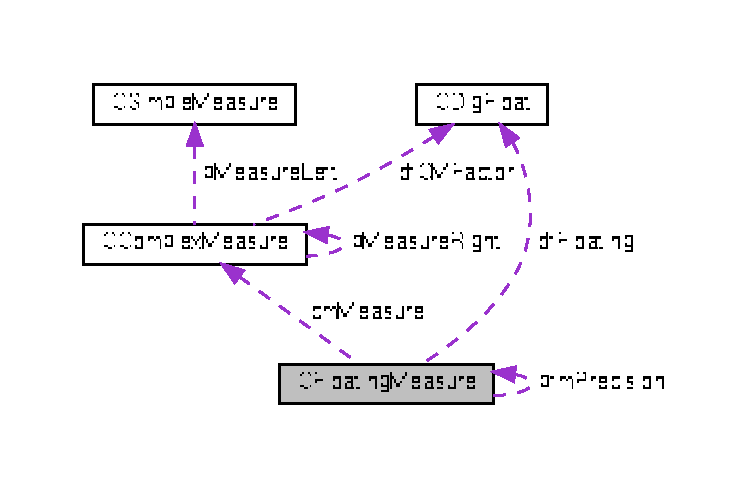
\includegraphics[width=350pt]{d5/d9a/classCFloatingMeasure__coll__graph}
\end{center}
\end{figure}
\subsection*{Public Member Functions}
\begin{DoxyCompactItemize}
\item 
\hyperlink{classCFloatingMeasure_aa30b4d0ea6b6bbc022717c875419fb44}{C\+Floating\+Measure} ()
\item 
\hyperlink{classCFloatingMeasure_ac5f28ce988a77d1bc8b34b361827788c}{C\+Floating\+Measure} (const \hyperlink{classCFloatingMeasure}{C\+Floating\+Measure} \&other)
\item 
\hyperlink{classCFloatingMeasure_a8ce55143653895584c3f578103308714}{C\+Floating\+Measure} (const \hyperlink{classCDigFloat}{C\+Dig\+Float} \&Other\+Floating, const \hyperlink{classCComplexMeasure}{C\+Complex\+Measure} \&Other\+Measure)
\begin{DoxyCompactList}\small\item\em Constructor from \hyperlink{classCDigFloat}{C\+Dig\+Float} and \hyperlink{classCComplexMeasure}{C\+Complex\+Measure}. \end{DoxyCompactList}\item 
\hyperlink{classCFloatingMeasure_a43c9d00b7a9e66da291926f58459c7c8}{$\sim$\+C\+Floating\+Measure} ()
\item 
\hyperlink{classCFloatingMeasure}{C\+Floating\+Measure} \& \hyperlink{classCFloatingMeasure_a958ef3d71c3dd7355bebef272df5b9e0}{operator=} (const \hyperlink{classCFloatingMeasure}{C\+Floating\+Measure} \&other)
\item 
bool \hyperlink{classCFloatingMeasure_ab4233b1232751f99e9e1f91f2ee55cc9}{operator==} (const \hyperlink{classCFloatingMeasure}{C\+Floating\+Measure} \&other) const
\begin{DoxyCompactList}\small\item\em comparison operator \end{DoxyCompactList}\item 
bool \hyperlink{classCFloatingMeasure_afbedc9a56acac7c6738357ce2347aad3}{operator!=} (const \hyperlink{classCFloatingMeasure}{C\+Floating\+Measure} \&other) const
\begin{DoxyCompactList}\small\item\em operator!= \end{DoxyCompactList}\item 
bool \hyperlink{classCFloatingMeasure_a35d506664a6a72856d56cbf18ea9d2a4}{operator$<$} (const \hyperlink{classCFloatingMeasure}{C\+Floating\+Measure} \&other) const
\begin{DoxyCompactList}\small\item\em operator$<$ \end{DoxyCompactList}\item 
bool \hyperlink{classCFloatingMeasure_ad8b94201f5df969de576f89a249c947e}{operator$<$=} (const \hyperlink{classCFloatingMeasure}{C\+Floating\+Measure} \&other) const
\begin{DoxyCompactList}\small\item\em operator$<$= \end{DoxyCompactList}\item 
bool \hyperlink{classCFloatingMeasure_aa6575f6f658ee524da9e5f123189cef1}{operator$>$=} (const \hyperlink{classCFloatingMeasure}{C\+Floating\+Measure} \&other) const
\begin{DoxyCompactList}\small\item\em operator$>$= \end{DoxyCompactList}\item 
bool \hyperlink{classCFloatingMeasure_a59cd04759c33941c7c20db3c81dcde14}{operator$>$} (const \hyperlink{classCFloatingMeasure}{C\+Floating\+Measure} \&other) const
\begin{DoxyCompactList}\small\item\em operator$>$ \end{DoxyCompactList}\item 
\hyperlink{classCFloatingMeasure}{C\+Floating\+Measure} \& \hyperlink{classCFloatingMeasure_a40f0ec4cb155856efed8db28c7c8fa3e}{operator+=} (const \hyperlink{classCFloatingMeasure}{C\+Floating\+Measure} \&other)
\begin{DoxyCompactList}\small\item\em operator += \end{DoxyCompactList}\item 
\hyperlink{classCFloatingMeasure}{C\+Floating\+Measure} \& \hyperlink{classCFloatingMeasure_a3661f71ed47a6659f7e27adff3c5c369}{operator-\/=} (const \hyperlink{classCFloatingMeasure}{C\+Floating\+Measure} \&other)
\begin{DoxyCompactList}\small\item\em operator-\/= \end{DoxyCompactList}\item 
\hyperlink{classCFloatingMeasure}{C\+Floating\+Measure} \& \hyperlink{classCFloatingMeasure_a2df7738d5c017a02c1f11c40809cac96}{operator$\ast$=} (const \hyperlink{classCFloatingMeasure}{C\+Floating\+Measure} \&other)
\begin{DoxyCompactList}\small\item\em operator$\ast$= \end{DoxyCompactList}\item 
\hyperlink{classCFloatingMeasure}{C\+Floating\+Measure} \& \hyperlink{classCFloatingMeasure_a1bc972be1fa5abd0619849710eef398c}{operator/=} (const \hyperlink{classCFloatingMeasure}{C\+Floating\+Measure} \&other)
\begin{DoxyCompactList}\small\item\em operator/= \end{DoxyCompactList}\item 
\hyperlink{classCFloatingMeasure}{C\+Floating\+Measure} \hyperlink{classCFloatingMeasure_a26560fcb587eafe8966541159eec57de}{operator+} (const \hyperlink{classCFloatingMeasure}{C\+Floating\+Measure} \&other)
\begin{DoxyCompactList}\small\item\em operator + \end{DoxyCompactList}\item 
\hyperlink{classCFloatingMeasure}{C\+Floating\+Measure} \hyperlink{classCFloatingMeasure_ad29973f56a38dda22fc9d66a16b13860}{operator-\/} (const \hyperlink{classCFloatingMeasure}{C\+Floating\+Measure} \&other)
\begin{DoxyCompactList}\small\item\em operator-\/ \end{DoxyCompactList}\item 
\hyperlink{classCFloatingMeasure}{C\+Floating\+Measure} \hyperlink{classCFloatingMeasure_a993623835ced24f74075861b2aab736e}{operator$\ast$} (const \hyperlink{classCFloatingMeasure}{C\+Floating\+Measure} \&other)
\begin{DoxyCompactList}\small\item\em operator$\ast$ \end{DoxyCompactList}\item 
\hyperlink{classCFloatingMeasure}{C\+Floating\+Measure} \hyperlink{classCFloatingMeasure_acb68f4d17606dc2312f4efabe877ab80}{operator/} (const \hyperlink{classCFloatingMeasure}{C\+Floating\+Measure} \&other)
\begin{DoxyCompactList}\small\item\em operator/ \end{DoxyCompactList}\item 
\hyperlink{classCFloatingMeasure}{C\+Floating\+Measure} \& \hyperlink{classCFloatingMeasure_a051879dde322060eb7695667dd38ab13}{operator$\ast$=} (const double \&other)
\begin{DoxyCompactList}\small\item\em operator$\ast$= \end{DoxyCompactList}\item 
\hyperlink{classCFloatingMeasure}{C\+Floating\+Measure} \& \hyperlink{classCFloatingMeasure_a2ba332fa822922d51866e4361db1677b}{operator/=} (const double \&other)
\begin{DoxyCompactList}\small\item\em operator/= \end{DoxyCompactList}\item 
\hyperlink{classCFloatingMeasure}{C\+Floating\+Measure} \hyperlink{classCFloatingMeasure_a31cedd2120675c56064e12556432f550}{operator$\ast$} (const double \&other)
\begin{DoxyCompactList}\small\item\em operator$\ast$ \end{DoxyCompactList}\item 
\hyperlink{classCFloatingMeasure}{C\+Floating\+Measure} \hyperlink{classCFloatingMeasure_ac39b5a05cce42097d4439627aaaaf94c}{operator/} (const double \&other)
\begin{DoxyCompactList}\small\item\em operator/ \end{DoxyCompactList}\item 
void \hyperlink{classCFloatingMeasure_af4e2cc6a78b8e0cda11df432902bde8a}{Normalize} ()
\begin{DoxyCompactList}\small\item\em convert to SI unit and remove premeasures != pm\+Ident \end{DoxyCompactList}\item 
void \hyperlink{classCFloatingMeasure_a47731afb871889ee7da5f84b40e3a27f}{Simplify} ()
\begin{DoxyCompactList}\small\item\em convert to SI unit and remove premeasures != pm\+Ident \end{DoxyCompactList}\item 
bool \hyperlink{classCFloatingMeasure_ae69672971857cf047c5bc7ab4b631b6c}{Compatible} (const \hyperlink{classCFloatingMeasure}{C\+Floating\+Measure} \&other)
\begin{DoxyCompactList}\small\item\em check measures for compatibility \end{DoxyCompactList}\item 
bool \hyperlink{classCFloatingMeasure_a5cf69c287abe4e2f65242e97093f7595}{Compatible} (const \hyperlink{classCComplexMeasure}{C\+Complex\+Measure} \&other)
\begin{DoxyCompactList}\small\item\em check measures for compatibility \end{DoxyCompactList}\item 
void \hyperlink{classCFloatingMeasure_aa0a16f8516d047576b588389504c0996}{Scale\+To} (const \hyperlink{classCFloatingMeasure}{C\+Floating\+Measure} \&other)
\begin{DoxyCompactList}\small\item\em scales to \hyperlink{classCComplexMeasure}{C\+Complex\+Measure} of other \end{DoxyCompactList}\item 
void \hyperlink{classCFloatingMeasure_a841b94d2883274e67999688fad40d538}{Scale\+To} (const \hyperlink{classCComplexMeasure}{C\+Complex\+Measure} \&other)
\begin{DoxyCompactList}\small\item\em scales to \hyperlink{classCComplexMeasure}{C\+Complex\+Measure} other \end{DoxyCompactList}\item 
void \hyperlink{classCFloatingMeasure_abaedeff78fb7009c788df5a016bc46d5}{Precision} (const \hyperlink{classCFloatingMeasure}{C\+Floating\+Measure} \&User\+Precision)
\begin{DoxyCompactList}\small\item\em setting precision of floating number by floating number\+: calls C\+Dig\+Float\+::\+Precision(n\+Digits) from \hyperlink{classCFloatingMeasure_aa0cec9966c6c08db75c493e44396cfc2}{C\+Floating\+Measure\+::df\+Floating}. \end{DoxyCompactList}\item 
void \hyperlink{classCFloatingMeasure_a4fe4d60589da6d4c7f09cb09fbea730b}{Precision\+Active} (const bool b\+Precision\+Active)
\begin{DoxyCompactList}\small\item\em switch precision defined by df\+Floating\+::n\+Precision on / off \end{DoxyCompactList}\item 
const bool \hyperlink{classCFloatingMeasure_a90d47ac476295db3c208cb484cd75764}{Precison\+Active} () const
\begin{DoxyCompactList}\small\item\em get Precision\+Active from df\+Floating \end{DoxyCompactList}\item 
bool \hyperlink{classCFloatingMeasure_a0ff3ae036cd2ee44d6b2eadc609b1d1a}{Valid} ()
\begin{DoxyCompactList}\small\item\em checks if the cm\+Measure and df\+Floating are valid values \end{DoxyCompactList}\item 
string \hyperlink{classCFloatingMeasure_a6d92f39204f23e81732cb77131517b6f}{Debug\+Out} ()
\begin{DoxyCompactList}\small\item\em debugging output for every member \end{DoxyCompactList}\item 
string \hyperlink{classCFloatingMeasure_af4caaa697967a257bc6e13117843ff58}{Print\+Short} ()
\begin{DoxyCompactList}\small\item\em printing short output\+: e.\+g. \char`\"{}10$\ast$mv/\+V\char`\"{} \end{DoxyCompactList}\item 
\hyperlink{classCDigFloat}{C\+Dig\+Float} \hyperlink{classCFloatingMeasure_ab41354d28783d125159bd6e9372c6d9f}{Floating} () const
\begin{DoxyCompactList}\small\item\em gettter for df\+Floating \end{DoxyCompactList}\item 
\hyperlink{classCComplexMeasure}{C\+Complex\+Measure} \hyperlink{classCFloatingMeasure_a8ac3af95a2619670a51d744c85b44463}{Measure} () const
\begin{DoxyCompactList}\small\item\em getter for cm\+Measure \end{DoxyCompactList}\item 
\hyperlink{classCFloatingMeasure}{C\+Floating\+Measure} \hyperlink{classCFloatingMeasure_ac8975daf37b98b3e996893e0de43c4eb}{Precision} () const
\begin{DoxyCompactList}\small\item\em get the precision as \hyperlink{classCFloatingMeasure}{C\+Floating\+Measure} \end{DoxyCompactList}\end{DoxyCompactItemize}
\subsection*{Protected Member Functions}
\begin{DoxyCompactItemize}
\item 
void \hyperlink{classCFloatingMeasure_a1e8a7467d6435c4cf349198804617623}{\+\_\+\+Init} ()
\begin{DoxyCompactList}\small\item\em initialization with invalid values\+: floating = my\+NaN, cm\+Measure = unknownn \end{DoxyCompactList}\item 
void \hyperlink{classCFloatingMeasure_a8e16f55f29d0d4c4148307a1f5953fe3}{\+\_\+\+Precision} (const \hyperlink{classCFloatingMeasure}{C\+Floating\+Measure} $\ast$p\+Other\+Precision)
\item 
void \hyperlink{classCFloatingMeasure_af35c54ac06b1c8ddca86390360559548}{Measure} (const \hyperlink{classCComplexMeasure}{C\+Complex\+Measure} \&other)
\begin{DoxyCompactList}\small\item\em setter for cm\+Measure \end{DoxyCompactList}\item 
void \hyperlink{classCFloatingMeasure_aa33fe952e9c01f5f76cef5e6f0d03864}{Floating} (const \hyperlink{classCDigFloat}{C\+Dig\+Float} \&other)
\begin{DoxyCompactList}\small\item\em setter for df\+Floating \end{DoxyCompactList}\end{DoxyCompactItemize}
\subsection*{Protected Attributes}
\begin{DoxyCompactItemize}
\item 
\hyperlink{classCComplexMeasure}{C\+Complex\+Measure} \hyperlink{classCFloatingMeasure_a3a23946016d1b7f41a1ecf05f4d5d5c6}{cm\+Measure}
\item 
\hyperlink{classCDigFloat}{C\+Dig\+Float} \hyperlink{classCFloatingMeasure_aa0cec9966c6c08db75c493e44396cfc2}{df\+Floating}
\item 
\hyperlink{classCFloatingMeasure}{C\+Floating\+Measure} $\ast$ \hyperlink{classCFloatingMeasure_a6bc7bd6e563e69cbf29692cd97153115}{pfm\+Precision}
\end{DoxyCompactItemize}
\subsection*{Friends}
\begin{DoxyCompactItemize}
\item 
class \hyperlink{classCFloatingMeasure_a2af9f0d4f7a8de5099b8d23df211b616}{C\+Complex\+Measure}
\end{DoxyCompactItemize}


\subsection{Detailed Description}
Floating\+Measure\+: represents a floating number with a complex measure (e.\+g. 10$\ast$m/s). This class offers\+: 


\begin{DoxyItemize}
\item operators (+,-\/,$\ast$,/,$<$=, $>$=, ==, !=, $<$, $>$)
\item simplification (e.\+g. 1$\ast$ms$\ast$10$\ast$m/s --$>$ 0.\+01m
\item normalization (i.\+e. SI units. e.\+g. 36$\ast$km/h --$>$ 10$\ast$m/s)
\item handling of the precision of the floating part for output and calculations 
\end{DoxyItemize}

Definition at line 39 of file Floating\+Measure.\+h.



\subsection{Constructor \& Destructor Documentation}
\mbox{\Hypertarget{classCFloatingMeasure_aa30b4d0ea6b6bbc022717c875419fb44}\label{classCFloatingMeasure_aa30b4d0ea6b6bbc022717c875419fb44}} 
\index{C\+Floating\+Measure@{C\+Floating\+Measure}!C\+Floating\+Measure@{C\+Floating\+Measure}}
\index{C\+Floating\+Measure@{C\+Floating\+Measure}!C\+Floating\+Measure@{C\+Floating\+Measure}}
\subsubsection{\texorpdfstring{C\+Floating\+Measure()}{CFloatingMeasure()}\hspace{0.1cm}{\footnotesize\ttfamily [1/3]}}
{\footnotesize\ttfamily C\+Floating\+Measure\+::\+C\+Floating\+Measure (\begin{DoxyParamCaption}{ }\end{DoxyParamCaption})}

Default constructor 

Definition at line 27 of file Floating\+Measure.\+cpp.



References \+\_\+\+Init().

\mbox{\Hypertarget{classCFloatingMeasure_ac5f28ce988a77d1bc8b34b361827788c}\label{classCFloatingMeasure_ac5f28ce988a77d1bc8b34b361827788c}} 
\index{C\+Floating\+Measure@{C\+Floating\+Measure}!C\+Floating\+Measure@{C\+Floating\+Measure}}
\index{C\+Floating\+Measure@{C\+Floating\+Measure}!C\+Floating\+Measure@{C\+Floating\+Measure}}
\subsubsection{\texorpdfstring{C\+Floating\+Measure()}{CFloatingMeasure()}\hspace{0.1cm}{\footnotesize\ttfamily [2/3]}}
{\footnotesize\ttfamily C\+Floating\+Measure\+::\+C\+Floating\+Measure (\begin{DoxyParamCaption}\item[{const \hyperlink{classCFloatingMeasure}{C\+Floating\+Measure} \&}]{other }\end{DoxyParamCaption})}

Copy constructor


\begin{DoxyParams}{Parameters}
{\em other} & \hyperlink{classCFloatingMeasure}{C\+Floating\+Measure} \\
\hline
\end{DoxyParams}


Definition at line 32 of file Floating\+Measure.\+cpp.



References \+\_\+\+Init(), \+\_\+\+Precision(), Floating(), Measure(), and pfm\+Precision.

\mbox{\Hypertarget{classCFloatingMeasure_a8ce55143653895584c3f578103308714}\label{classCFloatingMeasure_a8ce55143653895584c3f578103308714}} 
\index{C\+Floating\+Measure@{C\+Floating\+Measure}!C\+Floating\+Measure@{C\+Floating\+Measure}}
\index{C\+Floating\+Measure@{C\+Floating\+Measure}!C\+Floating\+Measure@{C\+Floating\+Measure}}
\subsubsection{\texorpdfstring{C\+Floating\+Measure()}{CFloatingMeasure()}\hspace{0.1cm}{\footnotesize\ttfamily [3/3]}}
{\footnotesize\ttfamily C\+Floating\+Measure\+::\+C\+Floating\+Measure (\begin{DoxyParamCaption}\item[{const \hyperlink{classCDigFloat}{C\+Dig\+Float} \&}]{Other\+Floating,  }\item[{const \hyperlink{classCComplexMeasure}{C\+Complex\+Measure} \&}]{Other\+Measure }\end{DoxyParamCaption})}



Constructor from \hyperlink{classCDigFloat}{C\+Dig\+Float} and \hyperlink{classCComplexMeasure}{C\+Complex\+Measure}. 


\begin{DoxyParams}{Parameters}
{\em Other\+Floating} & \+:\hyperlink{classCDigFloat}{C\+Dig\+Float} \\
\hline
{\em Other\+Measure} & \+:\hyperlink{classCComplexMeasure}{C\+Complex\+Measure} \\
\hline
\end{DoxyParams}


Definition at line 40 of file Floating\+Measure.\+cpp.



References \+\_\+\+Init(), Floating(), and Measure().

\mbox{\Hypertarget{classCFloatingMeasure_a43c9d00b7a9e66da291926f58459c7c8}\label{classCFloatingMeasure_a43c9d00b7a9e66da291926f58459c7c8}} 
\index{C\+Floating\+Measure@{C\+Floating\+Measure}!````~C\+Floating\+Measure@{$\sim$\+C\+Floating\+Measure}}
\index{````~C\+Floating\+Measure@{$\sim$\+C\+Floating\+Measure}!C\+Floating\+Measure@{C\+Floating\+Measure}}
\subsubsection{\texorpdfstring{$\sim$\+C\+Floating\+Measure()}{~CFloatingMeasure()}}
{\footnotesize\ttfamily C\+Floating\+Measure\+::$\sim$\+C\+Floating\+Measure (\begin{DoxyParamCaption}{ }\end{DoxyParamCaption})}

Destructor 

Definition at line 46 of file Floating\+Measure.\+cpp.



References pfm\+Precision, and Secure\+Delete\+Object\+Pointer().



\subsection{Member Function Documentation}
\mbox{\Hypertarget{classCFloatingMeasure_a1e8a7467d6435c4cf349198804617623}\label{classCFloatingMeasure_a1e8a7467d6435c4cf349198804617623}} 
\index{C\+Floating\+Measure@{C\+Floating\+Measure}!\+\_\+\+Init@{\+\_\+\+Init}}
\index{\+\_\+\+Init@{\+\_\+\+Init}!C\+Floating\+Measure@{C\+Floating\+Measure}}
\subsubsection{\texorpdfstring{\+\_\+\+Init()}{\_Init()}}
{\footnotesize\ttfamily void C\+Floating\+Measure\+::\+\_\+\+Init (\begin{DoxyParamCaption}{ }\end{DoxyParamCaption})\hspace{0.3cm}{\ttfamily [protected]}}



initialization with invalid values\+: floating = my\+NaN, cm\+Measure = unknownn 



Definition at line 289 of file Floating\+Measure.\+cpp.



References C\+Complex\+Measure\+::\+\_\+\+Init(), C\+Dig\+Float\+::\+\_\+\+Init(), cm\+Measure, df\+Floating, and pfm\+Precision.

\mbox{\Hypertarget{classCFloatingMeasure_a8e16f55f29d0d4c4148307a1f5953fe3}\label{classCFloatingMeasure_a8e16f55f29d0d4c4148307a1f5953fe3}} 
\index{C\+Floating\+Measure@{C\+Floating\+Measure}!\+\_\+\+Precision@{\+\_\+\+Precision}}
\index{\+\_\+\+Precision@{\+\_\+\+Precision}!C\+Floating\+Measure@{C\+Floating\+Measure}}
\subsubsection{\texorpdfstring{\+\_\+\+Precision()}{\_Precision()}}
{\footnotesize\ttfamily void C\+Floating\+Measure\+::\+\_\+\+Precision (\begin{DoxyParamCaption}\item[{const \hyperlink{classCFloatingMeasure}{C\+Floating\+Measure} $\ast$}]{p\+Other\+Precision }\end{DoxyParamCaption})\hspace{0.3cm}{\ttfamily [protected]}}



Definition at line 295 of file Floating\+Measure.\+cpp.



References pfm\+Precision, Precision(), and Secure\+Delete\+Object\+Pointer().

\mbox{\Hypertarget{classCFloatingMeasure_ae69672971857cf047c5bc7ab4b631b6c}\label{classCFloatingMeasure_ae69672971857cf047c5bc7ab4b631b6c}} 
\index{C\+Floating\+Measure@{C\+Floating\+Measure}!Compatible@{Compatible}}
\index{Compatible@{Compatible}!C\+Floating\+Measure@{C\+Floating\+Measure}}
\subsubsection{\texorpdfstring{Compatible()}{Compatible()}\hspace{0.1cm}{\footnotesize\ttfamily [1/2]}}
{\footnotesize\ttfamily bool C\+Floating\+Measure\+::\+Compatible (\begin{DoxyParamCaption}\item[{const \hyperlink{classCFloatingMeasure}{C\+Floating\+Measure} \&}]{other }\end{DoxyParamCaption})\hspace{0.3cm}{\ttfamily [inline]}}



check measures for compatibility 


\begin{DoxyParams}{Parameters}
{\em other} & p\+\_\+other\+:\hyperlink{classCFloatingMeasure}{C\+Floating\+Measure}\\
\hline
\end{DoxyParams}
\begin{DoxyReturn}{Returns}
bool 
\end{DoxyReturn}


Definition at line 241 of file Floating\+Measure.\+h.



References Measure().

\mbox{\Hypertarget{classCFloatingMeasure_a5cf69c287abe4e2f65242e97093f7595}\label{classCFloatingMeasure_a5cf69c287abe4e2f65242e97093f7595}} 
\index{C\+Floating\+Measure@{C\+Floating\+Measure}!Compatible@{Compatible}}
\index{Compatible@{Compatible}!C\+Floating\+Measure@{C\+Floating\+Measure}}
\subsubsection{\texorpdfstring{Compatible()}{Compatible()}\hspace{0.1cm}{\footnotesize\ttfamily [2/2]}}
{\footnotesize\ttfamily bool C\+Floating\+Measure\+::\+Compatible (\begin{DoxyParamCaption}\item[{const \hyperlink{classCComplexMeasure}{C\+Complex\+Measure} \&}]{other }\end{DoxyParamCaption})\hspace{0.3cm}{\ttfamily [inline]}}



check measures for compatibility 


\begin{DoxyParams}{Parameters}
{\em other} & p\+\_\+other\+:\hyperlink{classCComplexMeasure}{C\+Complex\+Measure}\&\\
\hline
\end{DoxyParams}
\begin{DoxyReturn}{Returns}
bool 
\end{DoxyReturn}


Definition at line 250 of file Floating\+Measure.\+h.



References C\+Complex\+Measure\+::\+Scale\+To().

\mbox{\Hypertarget{classCFloatingMeasure_a6d92f39204f23e81732cb77131517b6f}\label{classCFloatingMeasure_a6d92f39204f23e81732cb77131517b6f}} 
\index{C\+Floating\+Measure@{C\+Floating\+Measure}!Debug\+Out@{Debug\+Out}}
\index{Debug\+Out@{Debug\+Out}!C\+Floating\+Measure@{C\+Floating\+Measure}}
\subsubsection{\texorpdfstring{Debug\+Out()}{DebugOut()}}
{\footnotesize\ttfamily string C\+Floating\+Measure\+::\+Debug\+Out (\begin{DoxyParamCaption}{ }\end{DoxyParamCaption})}



debugging output for every member 

\begin{DoxyReturn}{Returns}
string 
\end{DoxyReturn}


Definition at line 311 of file Floating\+Measure.\+cpp.



References Bool2\+String(), cm\+Measure, C\+Complex\+Measure\+::\+Debug\+Out(), C\+Dig\+Float\+::\+Debug\+Out(), df\+Floating, pfm\+Precision, Print\+Short(), and Valid().

\mbox{\Hypertarget{classCFloatingMeasure_ab41354d28783d125159bd6e9372c6d9f}\label{classCFloatingMeasure_ab41354d28783d125159bd6e9372c6d9f}} 
\index{C\+Floating\+Measure@{C\+Floating\+Measure}!Floating@{Floating}}
\index{Floating@{Floating}!C\+Floating\+Measure@{C\+Floating\+Measure}}
\subsubsection{\texorpdfstring{Floating()}{Floating()}\hspace{0.1cm}{\footnotesize\ttfamily [1/2]}}
{\footnotesize\ttfamily \hyperlink{classCDigFloat}{C\+Dig\+Float} C\+Floating\+Measure\+::\+Floating (\begin{DoxyParamCaption}{ }\end{DoxyParamCaption}) const\hspace{0.3cm}{\ttfamily [inline]}}



gettter for df\+Floating 

\begin{DoxyReturn}{Returns}
\hyperlink{classCDigFloat}{C\+Dig\+Float} 
\end{DoxyReturn}


Definition at line 320 of file Floating\+Measure.\+h.

\mbox{\Hypertarget{classCFloatingMeasure_aa33fe952e9c01f5f76cef5e6f0d03864}\label{classCFloatingMeasure_aa33fe952e9c01f5f76cef5e6f0d03864}} 
\index{C\+Floating\+Measure@{C\+Floating\+Measure}!Floating@{Floating}}
\index{Floating@{Floating}!C\+Floating\+Measure@{C\+Floating\+Measure}}
\subsubsection{\texorpdfstring{Floating()}{Floating()}\hspace{0.1cm}{\footnotesize\ttfamily [2/2]}}
{\footnotesize\ttfamily void C\+Floating\+Measure\+::\+Floating (\begin{DoxyParamCaption}\item[{const \hyperlink{classCDigFloat}{C\+Dig\+Float} \&}]{other }\end{DoxyParamCaption})\hspace{0.3cm}{\ttfamily [inline]}, {\ttfamily [protected]}}



setter for df\+Floating 


\begin{DoxyParams}{Parameters}
{\em other} & p\+\_\+other\+:\hyperlink{classCDigFloat}{C\+Dig\+Float} \\
\hline
\end{DoxyParams}


Definition at line 361 of file Floating\+Measure.\+h.

\mbox{\Hypertarget{classCFloatingMeasure_a8ac3af95a2619670a51d744c85b44463}\label{classCFloatingMeasure_a8ac3af95a2619670a51d744c85b44463}} 
\index{C\+Floating\+Measure@{C\+Floating\+Measure}!Measure@{Measure}}
\index{Measure@{Measure}!C\+Floating\+Measure@{C\+Floating\+Measure}}
\subsubsection{\texorpdfstring{Measure()}{Measure()}\hspace{0.1cm}{\footnotesize\ttfamily [1/2]}}
{\footnotesize\ttfamily \hyperlink{classCComplexMeasure}{C\+Complex\+Measure} C\+Floating\+Measure\+::\+Measure (\begin{DoxyParamCaption}{ }\end{DoxyParamCaption}) const\hspace{0.3cm}{\ttfamily [inline]}}



getter for cm\+Measure 

\begin{DoxyReturn}{Returns}
\hyperlink{classCComplexMeasure}{C\+Complex\+Measure} 
\end{DoxyReturn}


Definition at line 326 of file Floating\+Measure.\+h.



References C\+Complex\+Measure\+::\+\_\+\+Init().

\mbox{\Hypertarget{classCFloatingMeasure_af35c54ac06b1c8ddca86390360559548}\label{classCFloatingMeasure_af35c54ac06b1c8ddca86390360559548}} 
\index{C\+Floating\+Measure@{C\+Floating\+Measure}!Measure@{Measure}}
\index{Measure@{Measure}!C\+Floating\+Measure@{C\+Floating\+Measure}}
\subsubsection{\texorpdfstring{Measure()}{Measure()}\hspace{0.1cm}{\footnotesize\ttfamily [2/2]}}
{\footnotesize\ttfamily void C\+Floating\+Measure\+::\+Measure (\begin{DoxyParamCaption}\item[{const \hyperlink{classCComplexMeasure}{C\+Complex\+Measure} \&}]{other }\end{DoxyParamCaption})\hspace{0.3cm}{\ttfamily [protected]}}



setter for cm\+Measure 


\begin{DoxyParams}{Parameters}
{\em other} & p\+\_\+other\+:\hyperlink{classCComplexMeasure}{C\+Complex\+Measure} \\
\hline
\end{DoxyParams}


Definition at line 245 of file Floating\+Measure.\+cpp.



References \+\_\+\+Precision(), cm\+Measure, and pfm\+Precision.

\mbox{\Hypertarget{classCFloatingMeasure_af4e2cc6a78b8e0cda11df432902bde8a}\label{classCFloatingMeasure_af4e2cc6a78b8e0cda11df432902bde8a}} 
\index{C\+Floating\+Measure@{C\+Floating\+Measure}!Normalize@{Normalize}}
\index{Normalize@{Normalize}!C\+Floating\+Measure@{C\+Floating\+Measure}}
\subsubsection{\texorpdfstring{Normalize()}{Normalize()}}
{\footnotesize\ttfamily void C\+Floating\+Measure\+::\+Normalize (\begin{DoxyParamCaption}{ }\end{DoxyParamCaption})}



convert to SI unit and remove premeasures != pm\+Ident 



Definition at line 204 of file Floating\+Measure.\+cpp.



References cm\+Measure, df\+Floating, C\+Complex\+Measure\+::\+Normalize(), and C\+Complex\+Measure\+::\+Release\+Exp10\+And\+Factor().

\mbox{\Hypertarget{classCFloatingMeasure_afbedc9a56acac7c6738357ce2347aad3}\label{classCFloatingMeasure_afbedc9a56acac7c6738357ce2347aad3}} 
\index{C\+Floating\+Measure@{C\+Floating\+Measure}!operator"!=@{operator"!=}}
\index{operator"!=@{operator"!=}!C\+Floating\+Measure@{C\+Floating\+Measure}}
\subsubsection{\texorpdfstring{operator"!=()}{operator!=()}}
{\footnotesize\ttfamily bool C\+Floating\+Measure\+::operator!= (\begin{DoxyParamCaption}\item[{const \hyperlink{classCFloatingMeasure}{C\+Floating\+Measure} \&}]{other }\end{DoxyParamCaption}) const}



operator!= 


\begin{DoxyParams}{Parameters}
{\em other} & p\+\_\+other\+:\hyperlink{classCFloatingMeasure}{C\+Floating\+Measure} \\
\hline
\end{DoxyParams}
\begin{DoxyReturn}{Returns}
bool 
\end{DoxyReturn}


Definition at line 71 of file Floating\+Measure.\+cpp.

\mbox{\Hypertarget{classCFloatingMeasure_a993623835ced24f74075861b2aab736e}\label{classCFloatingMeasure_a993623835ced24f74075861b2aab736e}} 
\index{C\+Floating\+Measure@{C\+Floating\+Measure}!operator$\ast$@{operator$\ast$}}
\index{operator$\ast$@{operator$\ast$}!C\+Floating\+Measure@{C\+Floating\+Measure}}
\subsubsection{\texorpdfstring{operator$\ast$()}{operator*()}\hspace{0.1cm}{\footnotesize\ttfamily [1/2]}}
{\footnotesize\ttfamily \hyperlink{classCFloatingMeasure}{C\+Floating\+Measure} C\+Floating\+Measure\+::operator$\ast$ (\begin{DoxyParamCaption}\item[{const \hyperlink{classCFloatingMeasure}{C\+Floating\+Measure} \&}]{other }\end{DoxyParamCaption})}



operator$\ast$ 


\begin{DoxyParams}{Parameters}
{\em other} & p\+\_\+other\+:\hyperlink{classCFloatingMeasure}{C\+Floating\+Measure} \\
\hline
\end{DoxyParams}
\begin{DoxyReturn}{Returns}
\hyperlink{classCFloatingMeasure}{C\+Floating\+Measure}\& 
\end{DoxyReturn}


Definition at line 164 of file Floating\+Measure.\+cpp.

\mbox{\Hypertarget{classCFloatingMeasure_a31cedd2120675c56064e12556432f550}\label{classCFloatingMeasure_a31cedd2120675c56064e12556432f550}} 
\index{C\+Floating\+Measure@{C\+Floating\+Measure}!operator$\ast$@{operator$\ast$}}
\index{operator$\ast$@{operator$\ast$}!C\+Floating\+Measure@{C\+Floating\+Measure}}
\subsubsection{\texorpdfstring{operator$\ast$()}{operator*()}\hspace{0.1cm}{\footnotesize\ttfamily [2/2]}}
{\footnotesize\ttfamily \hyperlink{classCFloatingMeasure}{C\+Floating\+Measure} C\+Floating\+Measure\+::operator$\ast$ (\begin{DoxyParamCaption}\item[{const double \&}]{other }\end{DoxyParamCaption})}



operator$\ast$ 


\begin{DoxyParams}{Parameters}
{\em other} & p\+\_\+other\+:double \\
\hline
\end{DoxyParams}
\begin{DoxyReturn}{Returns}
\hyperlink{classCFloatingMeasure}{C\+Floating\+Measure}\& 
\end{DoxyReturn}


Definition at line 190 of file Floating\+Measure.\+cpp.

\mbox{\Hypertarget{classCFloatingMeasure_a2df7738d5c017a02c1f11c40809cac96}\label{classCFloatingMeasure_a2df7738d5c017a02c1f11c40809cac96}} 
\index{C\+Floating\+Measure@{C\+Floating\+Measure}!operator$\ast$=@{operator$\ast$=}}
\index{operator$\ast$=@{operator$\ast$=}!C\+Floating\+Measure@{C\+Floating\+Measure}}
\subsubsection{\texorpdfstring{operator$\ast$=()}{operator*=()}\hspace{0.1cm}{\footnotesize\ttfamily [1/2]}}
{\footnotesize\ttfamily \hyperlink{classCFloatingMeasure}{C\+Floating\+Measure} \& C\+Floating\+Measure\+::operator$\ast$= (\begin{DoxyParamCaption}\item[{const \hyperlink{classCFloatingMeasure}{C\+Floating\+Measure} \&}]{other }\end{DoxyParamCaption})}



operator$\ast$= 


\begin{DoxyParams}{Parameters}
{\em other} & p\+\_\+other\+:\hyperlink{classCFloatingMeasure}{C\+Floating\+Measure} \\
\hline
\end{DoxyParams}
\begin{DoxyReturn}{Returns}
\hyperlink{classCFloatingMeasure}{C\+Floating\+Measure}\& 
\end{DoxyReturn}


Definition at line 136 of file Floating\+Measure.\+cpp.



References cm\+Measure, df\+Floating, Floating(), Measure(), and C\+Complex\+Measure\+::\+Release\+Exp10\+And\+Factor().

\mbox{\Hypertarget{classCFloatingMeasure_a051879dde322060eb7695667dd38ab13}\label{classCFloatingMeasure_a051879dde322060eb7695667dd38ab13}} 
\index{C\+Floating\+Measure@{C\+Floating\+Measure}!operator$\ast$=@{operator$\ast$=}}
\index{operator$\ast$=@{operator$\ast$=}!C\+Floating\+Measure@{C\+Floating\+Measure}}
\subsubsection{\texorpdfstring{operator$\ast$=()}{operator*=()}\hspace{0.1cm}{\footnotesize\ttfamily [2/2]}}
{\footnotesize\ttfamily \hyperlink{classCFloatingMeasure}{C\+Floating\+Measure} \& C\+Floating\+Measure\+::operator$\ast$= (\begin{DoxyParamCaption}\item[{const double \&}]{other }\end{DoxyParamCaption})}



operator$\ast$= 


\begin{DoxyParams}{Parameters}
{\em other} & p\+\_\+other\+:double \\
\hline
\end{DoxyParams}
\begin{DoxyReturn}{Returns}
\hyperlink{classCFloatingMeasure}{C\+Floating\+Measure}\& 
\end{DoxyReturn}


Definition at line 178 of file Floating\+Measure.\+cpp.



References df\+Floating.

\mbox{\Hypertarget{classCFloatingMeasure_a26560fcb587eafe8966541159eec57de}\label{classCFloatingMeasure_a26560fcb587eafe8966541159eec57de}} 
\index{C\+Floating\+Measure@{C\+Floating\+Measure}!operator+@{operator+}}
\index{operator+@{operator+}!C\+Floating\+Measure@{C\+Floating\+Measure}}
\subsubsection{\texorpdfstring{operator+()}{operator+()}}
{\footnotesize\ttfamily \hyperlink{classCFloatingMeasure}{C\+Floating\+Measure} C\+Floating\+Measure\+::operator+ (\begin{DoxyParamCaption}\item[{const \hyperlink{classCFloatingMeasure}{C\+Floating\+Measure} \&}]{other }\end{DoxyParamCaption})}



operator + 


\begin{DoxyParams}{Parameters}
{\em other} & p\+\_\+other\+:\hyperlink{classCFloatingMeasure}{C\+Floating\+Measure} \\
\hline
\end{DoxyParams}
\begin{DoxyReturn}{Returns}
\hyperlink{classCFloatingMeasure}{C\+Floating\+Measure}\& 
\end{DoxyReturn}


Definition at line 150 of file Floating\+Measure.\+cpp.

\mbox{\Hypertarget{classCFloatingMeasure_a40f0ec4cb155856efed8db28c7c8fa3e}\label{classCFloatingMeasure_a40f0ec4cb155856efed8db28c7c8fa3e}} 
\index{C\+Floating\+Measure@{C\+Floating\+Measure}!operator+=@{operator+=}}
\index{operator+=@{operator+=}!C\+Floating\+Measure@{C\+Floating\+Measure}}
\subsubsection{\texorpdfstring{operator+=()}{operator+=()}}
{\footnotesize\ttfamily \hyperlink{classCFloatingMeasure}{C\+Floating\+Measure} \& C\+Floating\+Measure\+::operator+= (\begin{DoxyParamCaption}\item[{const \hyperlink{classCFloatingMeasure}{C\+Floating\+Measure} \&}]{other }\end{DoxyParamCaption})}



operator += 


\begin{DoxyParams}{Parameters}
{\em other} & p\+\_\+other\+:\hyperlink{classCFloatingMeasure}{C\+Floating\+Measure} \\
\hline
\end{DoxyParams}
\begin{DoxyReturn}{Returns}
\hyperlink{classCFloatingMeasure}{C\+Floating\+Measure}\& 
\end{DoxyReturn}


Definition at line 103 of file Floating\+Measure.\+cpp.



References \+\_\+\+Init(), Compatible(), df\+Floating, Floating(), and Scale\+To().

\mbox{\Hypertarget{classCFloatingMeasure_ad29973f56a38dda22fc9d66a16b13860}\label{classCFloatingMeasure_ad29973f56a38dda22fc9d66a16b13860}} 
\index{C\+Floating\+Measure@{C\+Floating\+Measure}!operator-\/@{operator-\/}}
\index{operator-\/@{operator-\/}!C\+Floating\+Measure@{C\+Floating\+Measure}}
\subsubsection{\texorpdfstring{operator-\/()}{operator-()}}
{\footnotesize\ttfamily \hyperlink{classCFloatingMeasure}{C\+Floating\+Measure} C\+Floating\+Measure\+::operator-\/ (\begin{DoxyParamCaption}\item[{const \hyperlink{classCFloatingMeasure}{C\+Floating\+Measure} \&}]{other }\end{DoxyParamCaption})}



operator-\/ 


\begin{DoxyParams}{Parameters}
{\em other} & p\+\_\+other\+:\hyperlink{classCFloatingMeasure}{C\+Floating\+Measure} \\
\hline
\end{DoxyParams}
\begin{DoxyReturn}{Returns}
\hyperlink{classCFloatingMeasure}{C\+Floating\+Measure}\& 
\end{DoxyReturn}


Definition at line 157 of file Floating\+Measure.\+cpp.

\mbox{\Hypertarget{classCFloatingMeasure_a3661f71ed47a6659f7e27adff3c5c369}\label{classCFloatingMeasure_a3661f71ed47a6659f7e27adff3c5c369}} 
\index{C\+Floating\+Measure@{C\+Floating\+Measure}!operator-\/=@{operator-\/=}}
\index{operator-\/=@{operator-\/=}!C\+Floating\+Measure@{C\+Floating\+Measure}}
\subsubsection{\texorpdfstring{operator-\/=()}{operator-=()}}
{\footnotesize\ttfamily \hyperlink{classCFloatingMeasure}{C\+Floating\+Measure} \& C\+Floating\+Measure\+::operator-\/= (\begin{DoxyParamCaption}\item[{const \hyperlink{classCFloatingMeasure}{C\+Floating\+Measure} \&}]{other }\end{DoxyParamCaption})}



operator-\/= 


\begin{DoxyParams}{Parameters}
{\em other} & p\+\_\+other\+:\hyperlink{classCFloatingMeasure}{C\+Floating\+Measure} \\
\hline
\end{DoxyParams}
\begin{DoxyReturn}{Returns}
\hyperlink{classCFloatingMeasure}{C\+Floating\+Measure}\& 
\end{DoxyReturn}


Definition at line 119 of file Floating\+Measure.\+cpp.



References \+\_\+\+Init(), Compatible(), df\+Floating, Floating(), and Scale\+To().

\mbox{\Hypertarget{classCFloatingMeasure_acb68f4d17606dc2312f4efabe877ab80}\label{classCFloatingMeasure_acb68f4d17606dc2312f4efabe877ab80}} 
\index{C\+Floating\+Measure@{C\+Floating\+Measure}!operator/@{operator/}}
\index{operator/@{operator/}!C\+Floating\+Measure@{C\+Floating\+Measure}}
\subsubsection{\texorpdfstring{operator/()}{operator/()}\hspace{0.1cm}{\footnotesize\ttfamily [1/2]}}
{\footnotesize\ttfamily \hyperlink{classCFloatingMeasure}{C\+Floating\+Measure} C\+Floating\+Measure\+::operator/ (\begin{DoxyParamCaption}\item[{const \hyperlink{classCFloatingMeasure}{C\+Floating\+Measure} \&}]{other }\end{DoxyParamCaption})}



operator/ 


\begin{DoxyParams}{Parameters}
{\em other} & p\+\_\+other\+:\hyperlink{classCFloatingMeasure}{C\+Floating\+Measure} \\
\hline
\end{DoxyParams}
\begin{DoxyReturn}{Returns}
\hyperlink{classCFloatingMeasure}{C\+Floating\+Measure}\& 
\end{DoxyReturn}


Definition at line 171 of file Floating\+Measure.\+cpp.

\mbox{\Hypertarget{classCFloatingMeasure_ac39b5a05cce42097d4439627aaaaf94c}\label{classCFloatingMeasure_ac39b5a05cce42097d4439627aaaaf94c}} 
\index{C\+Floating\+Measure@{C\+Floating\+Measure}!operator/@{operator/}}
\index{operator/@{operator/}!C\+Floating\+Measure@{C\+Floating\+Measure}}
\subsubsection{\texorpdfstring{operator/()}{operator/()}\hspace{0.1cm}{\footnotesize\ttfamily [2/2]}}
{\footnotesize\ttfamily \hyperlink{classCFloatingMeasure}{C\+Floating\+Measure} C\+Floating\+Measure\+::operator/ (\begin{DoxyParamCaption}\item[{const double \&}]{other }\end{DoxyParamCaption})}



operator/ 


\begin{DoxyParams}{Parameters}
{\em other} & p\+\_\+other\+:double \\
\hline
\end{DoxyParams}
\begin{DoxyReturn}{Returns}
\hyperlink{classCFloatingMeasure}{C\+Floating\+Measure}\& 
\end{DoxyReturn}


Definition at line 197 of file Floating\+Measure.\+cpp.

\mbox{\Hypertarget{classCFloatingMeasure_a1bc972be1fa5abd0619849710eef398c}\label{classCFloatingMeasure_a1bc972be1fa5abd0619849710eef398c}} 
\index{C\+Floating\+Measure@{C\+Floating\+Measure}!operator/=@{operator/=}}
\index{operator/=@{operator/=}!C\+Floating\+Measure@{C\+Floating\+Measure}}
\subsubsection{\texorpdfstring{operator/=()}{operator/=()}\hspace{0.1cm}{\footnotesize\ttfamily [1/2]}}
{\footnotesize\ttfamily \hyperlink{classCFloatingMeasure}{C\+Floating\+Measure} \& C\+Floating\+Measure\+::operator/= (\begin{DoxyParamCaption}\item[{const \hyperlink{classCFloatingMeasure}{C\+Floating\+Measure} \&}]{other }\end{DoxyParamCaption})}



operator/= 


\begin{DoxyParams}{Parameters}
{\em other} & p\+\_\+other\+:\hyperlink{classCFloatingMeasure}{C\+Floating\+Measure} \\
\hline
\end{DoxyParams}
\begin{DoxyReturn}{Returns}
\hyperlink{classCFloatingMeasure}{C\+Floating\+Measure}\& 
\end{DoxyReturn}


Definition at line 143 of file Floating\+Measure.\+cpp.



References cm\+Measure, df\+Floating, Floating(), Measure(), and C\+Complex\+Measure\+::\+Release\+Exp10\+And\+Factor().

\mbox{\Hypertarget{classCFloatingMeasure_a2ba332fa822922d51866e4361db1677b}\label{classCFloatingMeasure_a2ba332fa822922d51866e4361db1677b}} 
\index{C\+Floating\+Measure@{C\+Floating\+Measure}!operator/=@{operator/=}}
\index{operator/=@{operator/=}!C\+Floating\+Measure@{C\+Floating\+Measure}}
\subsubsection{\texorpdfstring{operator/=()}{operator/=()}\hspace{0.1cm}{\footnotesize\ttfamily [2/2]}}
{\footnotesize\ttfamily \hyperlink{classCFloatingMeasure}{C\+Floating\+Measure} \& C\+Floating\+Measure\+::operator/= (\begin{DoxyParamCaption}\item[{const double \&}]{other }\end{DoxyParamCaption})}



operator/= 


\begin{DoxyParams}{Parameters}
{\em other} & p\+\_\+other\+:double \\
\hline
\end{DoxyParams}
\begin{DoxyReturn}{Returns}
\hyperlink{classCFloatingMeasure}{C\+Floating\+Measure}\& 
\end{DoxyReturn}


Definition at line 184 of file Floating\+Measure.\+cpp.



References df\+Floating.

\mbox{\Hypertarget{classCFloatingMeasure_a35d506664a6a72856d56cbf18ea9d2a4}\label{classCFloatingMeasure_a35d506664a6a72856d56cbf18ea9d2a4}} 
\index{C\+Floating\+Measure@{C\+Floating\+Measure}!operator$<$@{operator$<$}}
\index{operator$<$@{operator$<$}!C\+Floating\+Measure@{C\+Floating\+Measure}}
\subsubsection{\texorpdfstring{operator$<$()}{operator<()}}
{\footnotesize\ttfamily bool C\+Floating\+Measure\+::operator$<$ (\begin{DoxyParamCaption}\item[{const \hyperlink{classCFloatingMeasure}{C\+Floating\+Measure} \&}]{other }\end{DoxyParamCaption}) const}



operator$<$ 


\begin{DoxyParams}{Parameters}
{\em other} & p\+\_\+other\+:\hyperlink{classCFloatingMeasure}{C\+Floating\+Measure} \\
\hline
\end{DoxyParams}
\begin{DoxyReturn}{Returns}
bool 
\end{DoxyReturn}


Definition at line 75 of file Floating\+Measure.\+cpp.



References Floating(), and Scale\+To().

\mbox{\Hypertarget{classCFloatingMeasure_ad8b94201f5df969de576f89a249c947e}\label{classCFloatingMeasure_ad8b94201f5df969de576f89a249c947e}} 
\index{C\+Floating\+Measure@{C\+Floating\+Measure}!operator$<$=@{operator$<$=}}
\index{operator$<$=@{operator$<$=}!C\+Floating\+Measure@{C\+Floating\+Measure}}
\subsubsection{\texorpdfstring{operator$<$=()}{operator<=()}}
{\footnotesize\ttfamily bool C\+Floating\+Measure\+::operator$<$= (\begin{DoxyParamCaption}\item[{const \hyperlink{classCFloatingMeasure}{C\+Floating\+Measure} \&}]{other }\end{DoxyParamCaption}) const}



operator$<$= 


\begin{DoxyParams}{Parameters}
{\em other} & p\+\_\+other\+:\hyperlink{classCFloatingMeasure}{C\+Floating\+Measure} \\
\hline
\end{DoxyParams}
\begin{DoxyReturn}{Returns}
bool 
\end{DoxyReturn}


Definition at line 82 of file Floating\+Measure.\+cpp.



References Floating(), and Scale\+To().

\mbox{\Hypertarget{classCFloatingMeasure_a958ef3d71c3dd7355bebef272df5b9e0}\label{classCFloatingMeasure_a958ef3d71c3dd7355bebef272df5b9e0}} 
\index{C\+Floating\+Measure@{C\+Floating\+Measure}!operator=@{operator=}}
\index{operator=@{operator=}!C\+Floating\+Measure@{C\+Floating\+Measure}}
\subsubsection{\texorpdfstring{operator=()}{operator=()}}
{\footnotesize\ttfamily \hyperlink{classCFloatingMeasure}{C\+Floating\+Measure} \& C\+Floating\+Measure\+::operator= (\begin{DoxyParamCaption}\item[{const \hyperlink{classCFloatingMeasure}{C\+Floating\+Measure} \&}]{other }\end{DoxyParamCaption})}

Assignment operator


\begin{DoxyParams}{Parameters}
{\em other} & \hyperlink{classCFloatingMeasure}{C\+Floating\+Measure} \\
\hline
\end{DoxyParams}
\begin{DoxyReturn}{Returns}
\hyperlink{classCFloatingMeasure}{C\+Floating\+Measure} 
\end{DoxyReturn}


Definition at line 51 of file Floating\+Measure.\+cpp.



References \+\_\+\+Precision(), Floating(), Measure(), and pfm\+Precision.

\mbox{\Hypertarget{classCFloatingMeasure_ab4233b1232751f99e9e1f91f2ee55cc9}\label{classCFloatingMeasure_ab4233b1232751f99e9e1f91f2ee55cc9}} 
\index{C\+Floating\+Measure@{C\+Floating\+Measure}!operator==@{operator==}}
\index{operator==@{operator==}!C\+Floating\+Measure@{C\+Floating\+Measure}}
\subsubsection{\texorpdfstring{operator==()}{operator==()}}
{\footnotesize\ttfamily bool C\+Floating\+Measure\+::operator== (\begin{DoxyParamCaption}\item[{const \hyperlink{classCFloatingMeasure}{C\+Floating\+Measure} \&}]{other }\end{DoxyParamCaption}) const}



comparison operator 


\begin{DoxyParams}{Parameters}
{\em other} & p\+\_\+other\+:\hyperlink{classCFloatingMeasure}{C\+Floating\+Measure} \\
\hline
\end{DoxyParams}
\begin{DoxyReturn}{Returns}
bool 
\end{DoxyReturn}


Definition at line 60 of file Floating\+Measure.\+cpp.



References Floating(), Measure(), and Scale\+To().

\mbox{\Hypertarget{classCFloatingMeasure_a59cd04759c33941c7c20db3c81dcde14}\label{classCFloatingMeasure_a59cd04759c33941c7c20db3c81dcde14}} 
\index{C\+Floating\+Measure@{C\+Floating\+Measure}!operator$>$@{operator$>$}}
\index{operator$>$@{operator$>$}!C\+Floating\+Measure@{C\+Floating\+Measure}}
\subsubsection{\texorpdfstring{operator$>$()}{operator>()}}
{\footnotesize\ttfamily bool C\+Floating\+Measure\+::operator$>$ (\begin{DoxyParamCaption}\item[{const \hyperlink{classCFloatingMeasure}{C\+Floating\+Measure} \&}]{other }\end{DoxyParamCaption}) const}



operator$>$ 


\begin{DoxyParams}{Parameters}
{\em other} & p\+\_\+other\+:\hyperlink{classCFloatingMeasure}{C\+Floating\+Measure} \\
\hline
\end{DoxyParams}
\begin{DoxyReturn}{Returns}
bool 
\end{DoxyReturn}


Definition at line 96 of file Floating\+Measure.\+cpp.



References Floating(), and Scale\+To().

\mbox{\Hypertarget{classCFloatingMeasure_aa6575f6f658ee524da9e5f123189cef1}\label{classCFloatingMeasure_aa6575f6f658ee524da9e5f123189cef1}} 
\index{C\+Floating\+Measure@{C\+Floating\+Measure}!operator$>$=@{operator$>$=}}
\index{operator$>$=@{operator$>$=}!C\+Floating\+Measure@{C\+Floating\+Measure}}
\subsubsection{\texorpdfstring{operator$>$=()}{operator>=()}}
{\footnotesize\ttfamily bool C\+Floating\+Measure\+::operator$>$= (\begin{DoxyParamCaption}\item[{const \hyperlink{classCFloatingMeasure}{C\+Floating\+Measure} \&}]{other }\end{DoxyParamCaption}) const}



operator$>$= 


\begin{DoxyParams}{Parameters}
{\em other} & p\+\_\+other\+:\hyperlink{classCFloatingMeasure}{C\+Floating\+Measure} \\
\hline
\end{DoxyParams}
\begin{DoxyReturn}{Returns}
bool 
\end{DoxyReturn}


Definition at line 89 of file Floating\+Measure.\+cpp.



References Floating(), and Scale\+To().

\mbox{\Hypertarget{classCFloatingMeasure_abaedeff78fb7009c788df5a016bc46d5}\label{classCFloatingMeasure_abaedeff78fb7009c788df5a016bc46d5}} 
\index{C\+Floating\+Measure@{C\+Floating\+Measure}!Precision@{Precision}}
\index{Precision@{Precision}!C\+Floating\+Measure@{C\+Floating\+Measure}}
\subsubsection{\texorpdfstring{Precision()}{Precision()}\hspace{0.1cm}{\footnotesize\ttfamily [1/2]}}
{\footnotesize\ttfamily void C\+Floating\+Measure\+::\+Precision (\begin{DoxyParamCaption}\item[{const \hyperlink{classCFloatingMeasure}{C\+Floating\+Measure} \&}]{User\+Precision }\end{DoxyParamCaption})}



setting precision of floating number by floating number\+: calls C\+Dig\+Float\+::\+Precision(n\+Digits) from \hyperlink{classCFloatingMeasure_aa0cec9966c6c08db75c493e44396cfc2}{C\+Floating\+Measure\+::df\+Floating}. 


\begin{DoxyParams}{Parameters}
{\em User\+Precision} & \hyperlink{classCFloatingMeasure}{C\+Floating\+Measure} which determines no. of digits=(-\/log(User\+Precision) +1) \\
\hline
\end{DoxyParams}


Definition at line 254 of file Floating\+Measure.\+cpp.



References C\+Floating\+Measure(), df\+Floating, Floating(), Measure(), pfm\+Precision, C\+Dig\+Float\+::\+Precision(), C\+Dig\+Float\+::\+Raw\+Value(), Scale\+To(), and Valid().

\mbox{\Hypertarget{classCFloatingMeasure_ac8975daf37b98b3e996893e0de43c4eb}\label{classCFloatingMeasure_ac8975daf37b98b3e996893e0de43c4eb}} 
\index{C\+Floating\+Measure@{C\+Floating\+Measure}!Precision@{Precision}}
\index{Precision@{Precision}!C\+Floating\+Measure@{C\+Floating\+Measure}}
\subsubsection{\texorpdfstring{Precision()}{Precision()}\hspace{0.1cm}{\footnotesize\ttfamily [2/2]}}
{\footnotesize\ttfamily \hyperlink{classCFloatingMeasure}{C\+Floating\+Measure} C\+Floating\+Measure\+::\+Precision (\begin{DoxyParamCaption}{ }\end{DoxyParamCaption}) const}



get the precision as \hyperlink{classCFloatingMeasure}{C\+Floating\+Measure} 

\begin{DoxyReturn}{Returns}
\hyperlink{classCFloatingMeasure}{C\+Floating\+Measure} 
\end{DoxyReturn}


Definition at line 281 of file Floating\+Measure.\+cpp.



References pfm\+Precision.

\mbox{\Hypertarget{classCFloatingMeasure_a4fe4d60589da6d4c7f09cb09fbea730b}\label{classCFloatingMeasure_a4fe4d60589da6d4c7f09cb09fbea730b}} 
\index{C\+Floating\+Measure@{C\+Floating\+Measure}!Precision\+Active@{Precision\+Active}}
\index{Precision\+Active@{Precision\+Active}!C\+Floating\+Measure@{C\+Floating\+Measure}}
\subsubsection{\texorpdfstring{Precision\+Active()}{PrecisionActive()}}
{\footnotesize\ttfamily void C\+Floating\+Measure\+::\+Precision\+Active (\begin{DoxyParamCaption}\item[{const bool}]{b\+Precision\+Active }\end{DoxyParamCaption})\hspace{0.3cm}{\ttfamily [inline]}}



switch precision defined by df\+Floating\+::n\+Precision on / off 


\begin{DoxyParams}{Parameters}
{\em b\+Precision\+Active} & p\+\_\+b\+Precision\+Active\+:bool \\
\hline
\end{DoxyParams}


Definition at line 282 of file Floating\+Measure.\+h.

\mbox{\Hypertarget{classCFloatingMeasure_a90d47ac476295db3c208cb484cd75764}\label{classCFloatingMeasure_a90d47ac476295db3c208cb484cd75764}} 
\index{C\+Floating\+Measure@{C\+Floating\+Measure}!Precison\+Active@{Precison\+Active}}
\index{Precison\+Active@{Precison\+Active}!C\+Floating\+Measure@{C\+Floating\+Measure}}
\subsubsection{\texorpdfstring{Precison\+Active()}{PrecisonActive()}}
{\footnotesize\ttfamily const bool C\+Floating\+Measure\+::\+Precison\+Active (\begin{DoxyParamCaption}{ }\end{DoxyParamCaption}) const\hspace{0.3cm}{\ttfamily [inline]}}



get Precision\+Active from df\+Floating 

\begin{DoxyReturn}{Returns}
const bool 
\end{DoxyReturn}


Definition at line 288 of file Floating\+Measure.\+h.

\mbox{\Hypertarget{classCFloatingMeasure_af4caaa697967a257bc6e13117843ff58}\label{classCFloatingMeasure_af4caaa697967a257bc6e13117843ff58}} 
\index{C\+Floating\+Measure@{C\+Floating\+Measure}!Print\+Short@{Print\+Short}}
\index{Print\+Short@{Print\+Short}!C\+Floating\+Measure@{C\+Floating\+Measure}}
\subsubsection{\texorpdfstring{Print\+Short()}{PrintShort()}}
{\footnotesize\ttfamily string C\+Floating\+Measure\+::\+Print\+Short (\begin{DoxyParamCaption}{ }\end{DoxyParamCaption})}



printing short output\+: e.\+g. \char`\"{}10$\ast$mv/\+V\char`\"{} 

\begin{DoxyReturn}{Returns}
string 
\end{DoxyReturn}


Definition at line 305 of file Floating\+Measure.\+cpp.



References cm\+Measure, df\+Floating, C\+Dig\+Float\+::\+Print(), and C\+Complex\+Measure\+::\+Print\+All\+Short().

\mbox{\Hypertarget{classCFloatingMeasure_aa0a16f8516d047576b588389504c0996}\label{classCFloatingMeasure_aa0a16f8516d047576b588389504c0996}} 
\index{C\+Floating\+Measure@{C\+Floating\+Measure}!Scale\+To@{Scale\+To}}
\index{Scale\+To@{Scale\+To}!C\+Floating\+Measure@{C\+Floating\+Measure}}
\subsubsection{\texorpdfstring{Scale\+To()}{ScaleTo()}\hspace{0.1cm}{\footnotesize\ttfamily [1/2]}}
{\footnotesize\ttfamily void C\+Floating\+Measure\+::\+Scale\+To (\begin{DoxyParamCaption}\item[{const \hyperlink{classCFloatingMeasure}{C\+Floating\+Measure} \&}]{other }\end{DoxyParamCaption})}



scales to \hyperlink{classCComplexMeasure}{C\+Complex\+Measure} of other 


\begin{DoxyParams}{Parameters}
{\em other} & p\+\_\+other\+:\hyperlink{classCFloatingMeasure}{C\+Floating\+Measure} \\
\hline
\end{DoxyParams}


Definition at line 216 of file Floating\+Measure.\+cpp.



References \+\_\+\+Init(), cm\+Measure, Compatible(), df\+Floating, Measure(), C\+Complex\+Measure\+::\+Release\+Exp10\+And\+Factor(), and C\+Complex\+Measure\+::\+Scale\+To().

\mbox{\Hypertarget{classCFloatingMeasure_a841b94d2883274e67999688fad40d538}\label{classCFloatingMeasure_a841b94d2883274e67999688fad40d538}} 
\index{C\+Floating\+Measure@{C\+Floating\+Measure}!Scale\+To@{Scale\+To}}
\index{Scale\+To@{Scale\+To}!C\+Floating\+Measure@{C\+Floating\+Measure}}
\subsubsection{\texorpdfstring{Scale\+To()}{ScaleTo()}\hspace{0.1cm}{\footnotesize\ttfamily [2/2]}}
{\footnotesize\ttfamily void C\+Floating\+Measure\+::\+Scale\+To (\begin{DoxyParamCaption}\item[{const \hyperlink{classCComplexMeasure}{C\+Complex\+Measure} \&}]{other }\end{DoxyParamCaption})}



scales to \hyperlink{classCComplexMeasure}{C\+Complex\+Measure} other 


\begin{DoxyParams}{Parameters}
{\em other} & p\+\_\+other\+:\hyperlink{classCComplexMeasure}{C\+Complex\+Measure}\& \\
\hline
\end{DoxyParams}


Definition at line 230 of file Floating\+Measure.\+cpp.



References \+\_\+\+Init(), cm\+Measure, Compatible(), df\+Floating, C\+Complex\+Measure\+::\+Release\+Exp10\+And\+Factor(), and C\+Complex\+Measure\+::\+Scale\+To().

\mbox{\Hypertarget{classCFloatingMeasure_a47731afb871889ee7da5f84b40e3a27f}\label{classCFloatingMeasure_a47731afb871889ee7da5f84b40e3a27f}} 
\index{C\+Floating\+Measure@{C\+Floating\+Measure}!Simplify@{Simplify}}
\index{Simplify@{Simplify}!C\+Floating\+Measure@{C\+Floating\+Measure}}
\subsubsection{\texorpdfstring{Simplify()}{Simplify()}}
{\footnotesize\ttfamily void C\+Floating\+Measure\+::\+Simplify (\begin{DoxyParamCaption}{ }\end{DoxyParamCaption})}



convert to SI unit and remove premeasures != pm\+Ident 



Definition at line 210 of file Floating\+Measure.\+cpp.



References cm\+Measure, df\+Floating, C\+Complex\+Measure\+::\+Release\+Exp10\+And\+Factor(), and C\+Complex\+Measure\+::\+Simplify().

\mbox{\Hypertarget{classCFloatingMeasure_a0ff3ae036cd2ee44d6b2eadc609b1d1a}\label{classCFloatingMeasure_a0ff3ae036cd2ee44d6b2eadc609b1d1a}} 
\index{C\+Floating\+Measure@{C\+Floating\+Measure}!Valid@{Valid}}
\index{Valid@{Valid}!C\+Floating\+Measure@{C\+Floating\+Measure}}
\subsubsection{\texorpdfstring{Valid()}{Valid()}}
{\footnotesize\ttfamily bool C\+Floating\+Measure\+::\+Valid (\begin{DoxyParamCaption}{ }\end{DoxyParamCaption})\hspace{0.3cm}{\ttfamily [inline]}}



checks if the cm\+Measure and df\+Floating are valid values 

\begin{DoxyReturn}{Returns}
bool 
\end{DoxyReturn}


Definition at line 294 of file Floating\+Measure.\+h.



References C\+Complex\+Measure\+::\+Debug\+Out().



\subsection{Friends And Related Function Documentation}
\mbox{\Hypertarget{classCFloatingMeasure_a2af9f0d4f7a8de5099b8d23df211b616}\label{classCFloatingMeasure_a2af9f0d4f7a8de5099b8d23df211b616}} 
\index{C\+Floating\+Measure@{C\+Floating\+Measure}!C\+Complex\+Measure@{C\+Complex\+Measure}}
\index{C\+Complex\+Measure@{C\+Complex\+Measure}!C\+Floating\+Measure@{C\+Floating\+Measure}}
\subsubsection{\texorpdfstring{C\+Complex\+Measure}{CComplexMeasure}}
{\footnotesize\ttfamily friend class \hyperlink{classCComplexMeasure}{C\+Complex\+Measure}\hspace{0.3cm}{\ttfamily [friend]}}



Definition at line 41 of file Floating\+Measure.\+h.



\subsection{Member Data Documentation}
\mbox{\Hypertarget{classCFloatingMeasure_a3a23946016d1b7f41a1ecf05f4d5d5c6}\label{classCFloatingMeasure_a3a23946016d1b7f41a1ecf05f4d5d5c6}} 
\index{C\+Floating\+Measure@{C\+Floating\+Measure}!cm\+Measure@{cm\+Measure}}
\index{cm\+Measure@{cm\+Measure}!C\+Floating\+Measure@{C\+Floating\+Measure}}
\subsubsection{\texorpdfstring{cm\+Measure}{cmMeasure}}
{\footnotesize\ttfamily \hyperlink{classCComplexMeasure}{C\+Complex\+Measure} C\+Floating\+Measure\+::cm\+Measure\hspace{0.3cm}{\ttfamily [protected]}}



Definition at line 367 of file Floating\+Measure.\+h.

\mbox{\Hypertarget{classCFloatingMeasure_aa0cec9966c6c08db75c493e44396cfc2}\label{classCFloatingMeasure_aa0cec9966c6c08db75c493e44396cfc2}} 
\index{C\+Floating\+Measure@{C\+Floating\+Measure}!df\+Floating@{df\+Floating}}
\index{df\+Floating@{df\+Floating}!C\+Floating\+Measure@{C\+Floating\+Measure}}
\subsubsection{\texorpdfstring{df\+Floating}{dfFloating}}
{\footnotesize\ttfamily \hyperlink{classCDigFloat}{C\+Dig\+Float} C\+Floating\+Measure\+::df\+Floating\hspace{0.3cm}{\ttfamily [protected]}}



Definition at line 368 of file Floating\+Measure.\+h.

\mbox{\Hypertarget{classCFloatingMeasure_a6bc7bd6e563e69cbf29692cd97153115}\label{classCFloatingMeasure_a6bc7bd6e563e69cbf29692cd97153115}} 
\index{C\+Floating\+Measure@{C\+Floating\+Measure}!pfm\+Precision@{pfm\+Precision}}
\index{pfm\+Precision@{pfm\+Precision}!C\+Floating\+Measure@{C\+Floating\+Measure}}
\subsubsection{\texorpdfstring{pfm\+Precision}{pfmPrecision}}
{\footnotesize\ttfamily \hyperlink{classCFloatingMeasure}{C\+Floating\+Measure}$\ast$ C\+Floating\+Measure\+::pfm\+Precision\hspace{0.3cm}{\ttfamily [protected]}}



Definition at line 369 of file Floating\+Measure.\+h.



The documentation for this class was generated from the following files\+:\begin{DoxyCompactItemize}
\item 
Floating\+Measure/\+Floating\+Measure/\hyperlink{FloatingMeasure_8h}{Floating\+Measure.\+h}\item 
Floating\+Measure/\+Floating\+Measure/\hyperlink{FloatingMeasure_8cpp}{Floating\+Measure.\+cpp}\end{DoxyCompactItemize}

\hypertarget{classCMeasureOperator}{}\section{C\+Measure\+Operator Class Reference}
\label{classCMeasureOperator}\index{C\+Measure\+Operator@{C\+Measure\+Operator}}


\hyperlink{classCMeasureOperator}{C\+Measure\+Operator}\+: this class is actually unused ...  




{\ttfamily \#include $<$Measure\+Operator.\+h$>$}



Inheritance diagram for C\+Measure\+Operator\+:\nopagebreak
\begin{figure}[H]
\begin{center}
\leavevmode
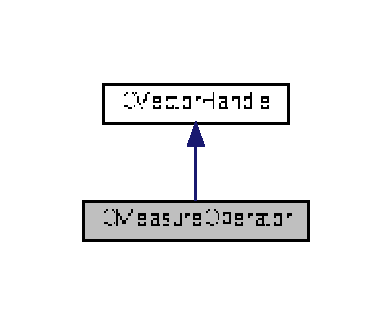
\includegraphics[width=188pt]{d4/dde/classCMeasureOperator__inherit__graph}
\end{center}
\end{figure}


Collaboration diagram for C\+Measure\+Operator\+:\nopagebreak
\begin{figure}[H]
\begin{center}
\leavevmode
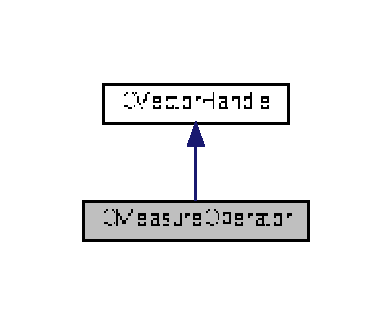
\includegraphics[width=188pt]{d2/dcf/classCMeasureOperator__coll__graph}
\end{center}
\end{figure}
\subsection*{Public Member Functions}
\begin{DoxyCompactItemize}
\item 
\hyperlink{classCMeasureOperator_abdf6e7568d2d9c5313299ff6b7a6012e}{C\+Measure\+Operator} ()
\item 
\hyperlink{classCMeasureOperator_acf2f26e41d5228767e4c098988cfaa89}{$\sim$\+C\+Measure\+Operator} ()
\end{DoxyCompactItemize}
\subsection*{Protected Member Functions}
\begin{DoxyCompactItemize}
\item 
virtual void \hyperlink{classCMeasureOperator_aa0d73fc93150362e4c7617f9ddb5e722}{\+\_\+\+Init} ()
\begin{DoxyCompactList}\small\item\em initialises long and short label by enum index e\+Operation \end{DoxyCompactList}\end{DoxyCompactItemize}
\subsection*{Additional Inherited Members}


\subsection{Detailed Description}
\hyperlink{classCMeasureOperator}{C\+Measure\+Operator}\+: this class is actually unused ... 

Definition at line 42 of file Measure\+Operator.\+h.



\subsection{Constructor \& Destructor Documentation}
\mbox{\Hypertarget{classCMeasureOperator_abdf6e7568d2d9c5313299ff6b7a6012e}\label{classCMeasureOperator_abdf6e7568d2d9c5313299ff6b7a6012e}} 
\index{C\+Measure\+Operator@{C\+Measure\+Operator}!C\+Measure\+Operator@{C\+Measure\+Operator}}
\index{C\+Measure\+Operator@{C\+Measure\+Operator}!C\+Measure\+Operator@{C\+Measure\+Operator}}
\subsubsection{\texorpdfstring{C\+Measure\+Operator()}{CMeasureOperator()}}
{\footnotesize\ttfamily C\+Measure\+Operator\+::\+C\+Measure\+Operator (\begin{DoxyParamCaption}{ }\end{DoxyParamCaption})}

Default constructor\+: calls \hyperlink{classCMeasureOperator_aa0d73fc93150362e4c7617f9ddb5e722}{\+\_\+\+Init()} 

Definition at line 27 of file Measure\+Operator.\+cpp.



References \+\_\+\+Init().

\mbox{\Hypertarget{classCMeasureOperator_acf2f26e41d5228767e4c098988cfaa89}\label{classCMeasureOperator_acf2f26e41d5228767e4c098988cfaa89}} 
\index{C\+Measure\+Operator@{C\+Measure\+Operator}!````~C\+Measure\+Operator@{$\sim$\+C\+Measure\+Operator}}
\index{````~C\+Measure\+Operator@{$\sim$\+C\+Measure\+Operator}!C\+Measure\+Operator@{C\+Measure\+Operator}}
\subsubsection{\texorpdfstring{$\sim$\+C\+Measure\+Operator()}{~CMeasureOperator()}}
{\footnotesize\ttfamily C\+Measure\+Operator\+::$\sim$\+C\+Measure\+Operator (\begin{DoxyParamCaption}{ }\end{DoxyParamCaption})}

Destructor 

Definition at line 32 of file Measure\+Operator.\+cpp.



\subsection{Member Function Documentation}
\mbox{\Hypertarget{classCMeasureOperator_aa0d73fc93150362e4c7617f9ddb5e722}\label{classCMeasureOperator_aa0d73fc93150362e4c7617f9ddb5e722}} 
\index{C\+Measure\+Operator@{C\+Measure\+Operator}!\+\_\+\+Init@{\+\_\+\+Init}}
\index{\+\_\+\+Init@{\+\_\+\+Init}!C\+Measure\+Operator@{C\+Measure\+Operator}}
\subsubsection{\texorpdfstring{\+\_\+\+Init()}{\_Init()}}
{\footnotesize\ttfamily void C\+Measure\+Operator\+::\+\_\+\+Init (\begin{DoxyParamCaption}{ }\end{DoxyParamCaption})\hspace{0.3cm}{\ttfamily [protected]}, {\ttfamily [virtual]}}



initialises long and short label by enum index e\+Operation 



Definition at line 36 of file Measure\+Operator.\+cpp.



References op\+Divide, op\+Last, op\+Mult, op\+Unknown, U\+N\+K\+N\+O\+W\+N\+\_\+\+L\+O\+NG, U\+N\+K\+N\+O\+W\+N\+\_\+\+S\+H\+O\+RT, C\+Vector\+Handle\+::vstr\+Long, and C\+Vector\+Handle\+::vstr\+Short.



The documentation for this class was generated from the following files\+:\begin{DoxyCompactItemize}
\item 
Floating\+Measure/\+Measure/\hyperlink{MeasureOperator_8h}{Measure\+Operator.\+h}\item 
Floating\+Measure/\+Measure/\hyperlink{MeasureOperator_8cpp}{Measure\+Operator.\+cpp}\end{DoxyCompactItemize}

\hypertarget{classCPreMeasure}{}\section{C\+Pre\+Measure Class Reference}
\label{classCPreMeasure}\index{C\+Pre\+Measure@{C\+Pre\+Measure}}


\hyperlink{classCPreMeasure}{C\+Pre\+Measure} represents the pre-\/measure part of a measure. ~\newline
 For example milli volt consists of the base-\/measure part \char`\"{}\+Volt\char`\"{} (see \hyperlink{classCBaseMeasure}{C\+Base\+Measure}) and the pre-\/measure part \char`\"{}milli\char`\"{}. ~\newline
 This class handles vectors of\+:  




{\ttfamily \#include $<$Pre\+Measure.\+h$>$}



Inheritance diagram for C\+Pre\+Measure\+:
\nopagebreak
\begin{figure}[H]
\begin{center}
\leavevmode
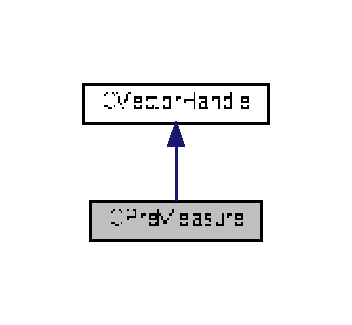
\includegraphics[width=169pt]{d9/da8/classCPreMeasure__inherit__graph}
\end{center}
\end{figure}


Collaboration diagram for C\+Pre\+Measure\+:
\nopagebreak
\begin{figure}[H]
\begin{center}
\leavevmode
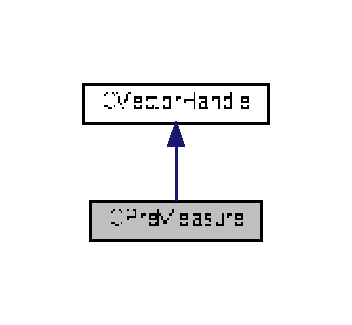
\includegraphics[width=169pt]{d4/d1d/classCPreMeasure__coll__graph}
\end{center}
\end{figure}
\subsection*{Public Member Functions}
\begin{DoxyCompactItemize}
\item 
\hyperlink{classCPreMeasure_acf40211e2818677f65b85f2db360c001}{C\+Pre\+Measure} ()
\begin{DoxyCompactList}\small\item\em default constructor\+: initialize all member vectors of \hyperlink{classCPreMeasure}{C\+Pre\+Measure}\+: \end{DoxyCompactList}\item 
\hyperlink{classCPreMeasure_ab927f07495fc7757c1488010f4440bc0}{$\sim$\+C\+Pre\+Measure} ()
\begin{DoxyCompactList}\small\item\em Destructor. \end{DoxyCompactList}\item 
string \hyperlink{classCPreMeasure_aa097540f3c74a3c616dee8ed1e120489}{Debug\+Out} (const int n\+Index)
\begin{DoxyCompactList}\small\item\em returns all representations in a string \end{DoxyCompactList}\item 
string \hyperlink{classCPreMeasure_a15f09957565ea1a5b4ca5975c1bbd76a}{Debug\+Out} (const \hyperlink{PreMeasure_8h_a6c81167b8d4c2badde42f81cb7214620}{e\+Pre\+Measure} Pre\+Measure\+Enum)
\begin{DoxyCompactList}\small\item\em returns all representations in a string \end{DoxyCompactList}\item 
int \hyperlink{classCPreMeasure_a1f6c35d76304a9eeb8105a53df63df0f}{Exp10} (const int n\+Exp10\+Idx)
\begin{DoxyCompactList}\small\item\em returns the exp10 (see \hyperlink{classCPreMeasure_a2c50eadae55427f0d77a013b3fab0fdb}{C\+Pre\+Measure\+::vn\+Exp10}) for a given pre-\/measure \end{DoxyCompactList}\item 
\hyperlink{PreMeasure_8h_a6c81167b8d4c2badde42f81cb7214620}{e\+Pre\+Measure} \hyperlink{classCPreMeasure_a6d9ee00647db5c9cb13e229c375096f8}{Get\+I\+D\+By\+Short\+Label} (const string \&str\+Short\+Label)
\begin{DoxyCompactList}\small\item\em returns the enum (index) of the pre-\/measure by searching the vstr\+Short \end{DoxyCompactList}\item 
\hyperlink{PreMeasure_8h_a6c81167b8d4c2badde42f81cb7214620}{e\+Pre\+Measure} \hyperlink{classCPreMeasure_a5c47dca5a6bc34def68e6a2c7b4c5caa}{Get\+I\+D\+By\+Long\+Label} (const string \&str\+Long\+Label)
\begin{DoxyCompactList}\small\item\em returns the enum (index) of the pre-\/measure by searching the vstr\+Long \end{DoxyCompactList}\item 
\hyperlink{PreMeasure_8h_a6c81167b8d4c2badde42f81cb7214620}{e\+Pre\+Measure} \hyperlink{classCPreMeasure_a90984e3bfb9676fca033289504d10219}{Get\+I\+D\+By\+Factor} (const double d\+Pre\+Measure\+Factor)
\begin{DoxyCompactList}\small\item\em returns the enum (index) of the pre-\/measure by searching the vd\+Factor \end{DoxyCompactList}\item 
\hyperlink{PreMeasure_8h_a6c81167b8d4c2badde42f81cb7214620}{e\+Pre\+Measure} \hyperlink{classCPreMeasure_a4f198103711ef15bac65a5011f32923e}{Get\+I\+D\+By\+Exp10} (const int n\+Exp10)
\begin{DoxyCompactList}\small\item\em returns the enum (index) of the pre-\/measure by searching the vn\+Exp10 \end{DoxyCompactList}\end{DoxyCompactItemize}
\subsection*{Protected Attributes}
\begin{DoxyCompactItemize}
\item 
vector$<$ int $>$ $\ast$ \hyperlink{classCPreMeasure_a2c50eadae55427f0d77a013b3fab0fdb}{vn\+Exp10}
\begin{DoxyCompactList}\small\item\em the exponents to the base of 10 (exp10 from now on) of the corresponding factors stored in \hyperlink{classCVectorHandle_af8f8b2e0da8363e695872ca85f33364e}{C\+Vector\+Handle\+::vd\+Factor} \end{DoxyCompactList}\end{DoxyCompactItemize}


\subsection{Detailed Description}
\hyperlink{classCPreMeasure}{C\+Pre\+Measure} represents the pre-\/measure part of a measure. ~\newline
 For example milli volt consists of the base-\/measure part \char`\"{}\+Volt\char`\"{} (see \hyperlink{classCBaseMeasure}{C\+Base\+Measure}) and the pre-\/measure part \char`\"{}milli\char`\"{}. ~\newline
 This class handles vectors of\+: 


\begin{DoxyItemize}
\item pre-\/measure factor (e.\+g. for \char`\"{}milli\char`\"{} with index \hyperlink{PreMeasure_8h_a6c81167b8d4c2badde42f81cb7214620aff93812e5c2f401cb10fe430a1d341f4}{pm\+Milli} the factor is 0.\+001)
\item the exponent to the base of 10 of the pre-\/measure factor (e.\+g. for \char`\"{}milli\char`\"{} the exp10 is -\/3)
\item the short label (e.\+g. for \char`\"{}milli\char`\"{} the short label is \char`\"{}m\char`\"{})
\item the long label (e.\+g. for \char`\"{}milli\char`\"{} the long label is \char`\"{}milli\char`\"{})~\newline
 These vectors are accessed by the indices defined by the enum \hyperlink{PreMeasure_8h_a6c81167b8d4c2badde42f81cb7214620}{e\+Pre\+Measure}.~\newline
 The indices can be vice versa accessed by
\item pre-\/measure factor
\item exp10
\item short label
\item long label 
\end{DoxyItemize}

Definition at line 75 of file Pre\+Measure.\+h.



\subsection{Constructor \& Destructor Documentation}
\mbox{\Hypertarget{classCPreMeasure_acf40211e2818677f65b85f2db360c001}\label{classCPreMeasure_acf40211e2818677f65b85f2db360c001}} 
\index{C\+Pre\+Measure@{C\+Pre\+Measure}!C\+Pre\+Measure@{C\+Pre\+Measure}}
\index{C\+Pre\+Measure@{C\+Pre\+Measure}!C\+Pre\+Measure@{C\+Pre\+Measure}}
\subsubsection{\texorpdfstring{C\+Pre\+Measure()}{CPreMeasure()}}
{\footnotesize\ttfamily C\+Pre\+Measure\+::\+C\+Pre\+Measure (\begin{DoxyParamCaption}{ }\end{DoxyParamCaption})}



default constructor\+: initialize all member vectors of \hyperlink{classCPreMeasure}{C\+Pre\+Measure}\+: 


\begin{DoxyItemize}
\item \hyperlink{classCVectorHandle_af8f8b2e0da8363e695872ca85f33364e}{C\+Pre\+Measure\+::vd\+Factor}
\item \hyperlink{classCPreMeasure_a2c50eadae55427f0d77a013b3fab0fdb}{C\+Pre\+Measure\+::vn\+Exp10}
\item \hyperlink{classCVectorHandle_afb50c8a33d4cf70bf92c644dca409ea2}{C\+Pre\+Measure\+::vstr\+Short}
\item \hyperlink{classCVectorHandle_a71bec0e385b9ca8e5ffa174b559da9f8}{C\+Pre\+Measure\+::vstr\+Long} 
\end{DoxyItemize}

Definition at line 27 of file Pre\+Measure.\+cpp.



References I\+N\+V\+A\+L\+I\+D\+\_\+\+E\+X\+P\+O\+N\+E\+NT, mu, pm\+Centi, pm\+Deca, pm\+Deci, pm\+Exa, pm\+Femto, pm\+Giga, pm\+Hecto, pm\+Ident, pm\+Kilo, pm\+Last, pm\+Mega, pm\+Micro, pm\+Milli, pm\+Nano, pm\+Peta, pm\+Piko, pm\+Tera, pm\+Unknown, pm\+Yotta, pm\+Zetta, U\+N\+K\+N\+O\+W\+N\+\_\+\+L\+O\+NG, U\+N\+K\+N\+O\+W\+N\+\_\+\+S\+H\+O\+RT, C\+Vector\+Handle\+::vd\+Factor, vn\+Exp10, C\+Vector\+Handle\+::vstr\+Long, and C\+Vector\+Handle\+::vstr\+Short.

\mbox{\Hypertarget{classCPreMeasure_ab927f07495fc7757c1488010f4440bc0}\label{classCPreMeasure_ab927f07495fc7757c1488010f4440bc0}} 
\index{C\+Pre\+Measure@{C\+Pre\+Measure}!````~C\+Pre\+Measure@{$\sim$\+C\+Pre\+Measure}}
\index{````~C\+Pre\+Measure@{$\sim$\+C\+Pre\+Measure}!C\+Pre\+Measure@{C\+Pre\+Measure}}
\subsubsection{\texorpdfstring{$\sim$\+C\+Pre\+Measure()}{~CPreMeasure()}}
{\footnotesize\ttfamily C\+Pre\+Measure\+::$\sim$\+C\+Pre\+Measure (\begin{DoxyParamCaption}{ }\end{DoxyParamCaption})}



Destructor. 



Definition at line 135 of file Pre\+Measure.\+cpp.



References Secure\+Delete\+Object\+Pointer(), and vn\+Exp10.



\subsection{Member Function Documentation}
\mbox{\Hypertarget{classCPreMeasure_aa097540f3c74a3c616dee8ed1e120489}\label{classCPreMeasure_aa097540f3c74a3c616dee8ed1e120489}} 
\index{C\+Pre\+Measure@{C\+Pre\+Measure}!Debug\+Out@{Debug\+Out}}
\index{Debug\+Out@{Debug\+Out}!C\+Pre\+Measure@{C\+Pre\+Measure}}
\subsubsection{\texorpdfstring{Debug\+Out()}{DebugOut()}\hspace{0.1cm}{\footnotesize\ttfamily [1/2]}}
{\footnotesize\ttfamily string C\+Pre\+Measure\+::\+Debug\+Out (\begin{DoxyParamCaption}\item[{const int}]{n\+Index }\end{DoxyParamCaption})}



returns all representations in a string 

\begin{DoxyReturn}{Returns}
string\+: output string 
\end{DoxyReturn}


Definition at line 200 of file Pre\+Measure.\+cpp.



References C\+Vector\+Handle\+::\+Factor(), C\+Vector\+Handle\+::\+Long(), and C\+Vector\+Handle\+::\+Short().

\mbox{\Hypertarget{classCPreMeasure_a15f09957565ea1a5b4ca5975c1bbd76a}\label{classCPreMeasure_a15f09957565ea1a5b4ca5975c1bbd76a}} 
\index{C\+Pre\+Measure@{C\+Pre\+Measure}!Debug\+Out@{Debug\+Out}}
\index{Debug\+Out@{Debug\+Out}!C\+Pre\+Measure@{C\+Pre\+Measure}}
\subsubsection{\texorpdfstring{Debug\+Out()}{DebugOut()}\hspace{0.1cm}{\footnotesize\ttfamily [2/2]}}
{\footnotesize\ttfamily string C\+Pre\+Measure\+::\+Debug\+Out (\begin{DoxyParamCaption}\item[{const \hyperlink{PreMeasure_8h_a6c81167b8d4c2badde42f81cb7214620}{e\+Pre\+Measure}}]{Pre\+Measure\+Enum }\end{DoxyParamCaption})}



returns all representations in a string 


\begin{DoxyParams}{Parameters}
{\em Pre\+Measure\+Enum} & p\+\_\+\+Pre\+Measure\+Enum\+:... \\
\hline
\end{DoxyParams}
\begin{DoxyReturn}{Returns}
string 
\end{DoxyReturn}


Definition at line 207 of file Pre\+Measure.\+cpp.



References Debug\+Out().

\mbox{\Hypertarget{classCPreMeasure_a1f6c35d76304a9eeb8105a53df63df0f}\label{classCPreMeasure_a1f6c35d76304a9eeb8105a53df63df0f}} 
\index{C\+Pre\+Measure@{C\+Pre\+Measure}!Exp10@{Exp10}}
\index{Exp10@{Exp10}!C\+Pre\+Measure@{C\+Pre\+Measure}}
\subsubsection{\texorpdfstring{Exp10()}{Exp10()}}
{\footnotesize\ttfamily int C\+Pre\+Measure\+::\+Exp10 (\begin{DoxyParamCaption}\item[{const int}]{n\+Exp10\+Idx }\end{DoxyParamCaption})\hspace{0.3cm}{\ttfamily [inline]}}



returns the exp10 (see \hyperlink{classCPreMeasure_a2c50eadae55427f0d77a013b3fab0fdb}{C\+Pre\+Measure\+::vn\+Exp10}) for a given pre-\/measure 


\begin{DoxyParams}{Parameters}
{\em n\+Exp10\+Idx} & p\+\_\+n\+Exp10\+Idx\+: is e.\+g. e\+Pre\+Measure\+::pm\+Milli (returns -\/3 in this case) \\
\hline
\end{DoxyParams}
\begin{DoxyReturn}{Returns}
int 
\end{DoxyReturn}


Definition at line 125 of file Pre\+Measure.\+h.



References Get\+Element\+From\+Vector\+By\+Index().

\mbox{\Hypertarget{classCPreMeasure_a4f198103711ef15bac65a5011f32923e}\label{classCPreMeasure_a4f198103711ef15bac65a5011f32923e}} 
\index{C\+Pre\+Measure@{C\+Pre\+Measure}!Get\+I\+D\+By\+Exp10@{Get\+I\+D\+By\+Exp10}}
\index{Get\+I\+D\+By\+Exp10@{Get\+I\+D\+By\+Exp10}!C\+Pre\+Measure@{C\+Pre\+Measure}}
\subsubsection{\texorpdfstring{Get\+I\+D\+By\+Exp10()}{GetIDByExp10()}}
{\footnotesize\ttfamily \hyperlink{PreMeasure_8h_a6c81167b8d4c2badde42f81cb7214620}{e\+Pre\+Measure} C\+Pre\+Measure\+::\+Get\+I\+D\+By\+Exp10 (\begin{DoxyParamCaption}\item[{const int}]{n\+Exp10 }\end{DoxyParamCaption})}



returns the enum (index) of the pre-\/measure by searching the vn\+Exp10 


\begin{DoxyParams}{Parameters}
{\em n\+Exp10} & \$\{p\+\_\+n\+Exp10\+:...\} \\
\hline
\end{DoxyParams}
\begin{DoxyReturn}{Returns}
e\+Pre\+Measure 
\end{DoxyReturn}


Definition at line 183 of file Pre\+Measure.\+cpp.



References abs(), Exp10(), pm\+First, and vn\+Exp10.

\mbox{\Hypertarget{classCPreMeasure_a90984e3bfb9676fca033289504d10219}\label{classCPreMeasure_a90984e3bfb9676fca033289504d10219}} 
\index{C\+Pre\+Measure@{C\+Pre\+Measure}!Get\+I\+D\+By\+Factor@{Get\+I\+D\+By\+Factor}}
\index{Get\+I\+D\+By\+Factor@{Get\+I\+D\+By\+Factor}!C\+Pre\+Measure@{C\+Pre\+Measure}}
\subsubsection{\texorpdfstring{Get\+I\+D\+By\+Factor()}{GetIDByFactor()}}
{\footnotesize\ttfamily \hyperlink{PreMeasure_8h_a6c81167b8d4c2badde42f81cb7214620}{e\+Pre\+Measure} C\+Pre\+Measure\+::\+Get\+I\+D\+By\+Factor (\begin{DoxyParamCaption}\item[{const double}]{d\+Pre\+Measure\+Factor }\end{DoxyParamCaption})}



returns the enum (index) of the pre-\/measure by searching the vd\+Factor 


\begin{DoxyParams}{Parameters}
{\em d\+Pre\+Measure\+Factor} & p\+\_\+d\+Pre\+Measure\+Factor\+: user given factor (e.\+g. 0.\+001 returns e\+Pre\+Measure\+::pm\+Milli) \\
\hline
\end{DoxyParams}
\begin{DoxyReturn}{Returns}
e\+Pre\+Measure 
\end{DoxyReturn}


Definition at line 142 of file Pre\+Measure.\+cpp.



References C\+Vector\+Handle\+::\+Factor(), pm\+First, pm\+Last, pm\+Unknown, and C\+Vector\+Handle\+::vd\+Factor.

\mbox{\Hypertarget{classCPreMeasure_a5c47dca5a6bc34def68e6a2c7b4c5caa}\label{classCPreMeasure_a5c47dca5a6bc34def68e6a2c7b4c5caa}} 
\index{C\+Pre\+Measure@{C\+Pre\+Measure}!Get\+I\+D\+By\+Long\+Label@{Get\+I\+D\+By\+Long\+Label}}
\index{Get\+I\+D\+By\+Long\+Label@{Get\+I\+D\+By\+Long\+Label}!C\+Pre\+Measure@{C\+Pre\+Measure}}
\subsubsection{\texorpdfstring{Get\+I\+D\+By\+Long\+Label()}{GetIDByLongLabel()}}
{\footnotesize\ttfamily \hyperlink{PreMeasure_8h_a6c81167b8d4c2badde42f81cb7214620}{e\+Pre\+Measure} C\+Pre\+Measure\+::\+Get\+I\+D\+By\+Long\+Label (\begin{DoxyParamCaption}\item[{const string \&}]{str\+Long\+Label }\end{DoxyParamCaption})\hspace{0.3cm}{\ttfamily [inline]}}



returns the enum (index) of the pre-\/measure by searching the vstr\+Long 


\begin{DoxyParams}{Parameters}
{\em str\+Long\+Label} & long label of the enum (e.\+g. \char`\"{}milli\char`\"{} \\
\hline
\end{DoxyParams}
\begin{DoxyReturn}{Returns}
e\+Pre\+Measure\+: the pre-\/measure index (e.\+g. e\+Pre\+Measure\+::pm\+Milli) 
\end{DoxyReturn}


Definition at line 150 of file Pre\+Measure.\+h.



References C\+Vector\+Handle\+::\+Get\+Index\+By\+Long\+Label().

\mbox{\Hypertarget{classCPreMeasure_a6d9ee00647db5c9cb13e229c375096f8}\label{classCPreMeasure_a6d9ee00647db5c9cb13e229c375096f8}} 
\index{C\+Pre\+Measure@{C\+Pre\+Measure}!Get\+I\+D\+By\+Short\+Label@{Get\+I\+D\+By\+Short\+Label}}
\index{Get\+I\+D\+By\+Short\+Label@{Get\+I\+D\+By\+Short\+Label}!C\+Pre\+Measure@{C\+Pre\+Measure}}
\subsubsection{\texorpdfstring{Get\+I\+D\+By\+Short\+Label()}{GetIDByShortLabel()}}
{\footnotesize\ttfamily \hyperlink{PreMeasure_8h_a6c81167b8d4c2badde42f81cb7214620}{e\+Pre\+Measure} C\+Pre\+Measure\+::\+Get\+I\+D\+By\+Short\+Label (\begin{DoxyParamCaption}\item[{const string \&}]{str\+Short\+Label }\end{DoxyParamCaption})\hspace{0.3cm}{\ttfamily [inline]}}



returns the enum (index) of the pre-\/measure by searching the vstr\+Short 


\begin{DoxyParams}{Parameters}
{\em str\+Short\+Label} & short label of the enum (e.\+g. \char`\"{}m\char`\"{} returns e\+Pre\+Measure\+::pm\+Milli) \\
\hline
\end{DoxyParams}
\begin{DoxyReturn}{Returns}
e\+Pre\+Measure 
\end{DoxyReturn}


Definition at line 139 of file Pre\+Measure.\+h.



References C\+Vector\+Handle\+::\+Get\+Index\+By\+Short\+Label().



\subsection{Member Data Documentation}
\mbox{\Hypertarget{classCPreMeasure_a2c50eadae55427f0d77a013b3fab0fdb}\label{classCPreMeasure_a2c50eadae55427f0d77a013b3fab0fdb}} 
\index{C\+Pre\+Measure@{C\+Pre\+Measure}!vn\+Exp10@{vn\+Exp10}}
\index{vn\+Exp10@{vn\+Exp10}!C\+Pre\+Measure@{C\+Pre\+Measure}}
\subsubsection{\texorpdfstring{vn\+Exp10}{vnExp10}}
{\footnotesize\ttfamily vector$<$int$>$$\ast$ C\+Pre\+Measure\+::vn\+Exp10\hspace{0.3cm}{\ttfamily [protected]}}



the exponents to the base of 10 (exp10 from now on) of the corresponding factors stored in \hyperlink{classCVectorHandle_af8f8b2e0da8363e695872ca85f33364e}{C\+Vector\+Handle\+::vd\+Factor} 



Definition at line 178 of file Pre\+Measure.\+h.



The documentation for this class was generated from the following files\+:\begin{DoxyCompactItemize}
\item 
Floating\+Measure/\+Measure/\hyperlink{PreMeasure_8h}{Pre\+Measure.\+h}\item 
Floating\+Measure/\+Measure/\hyperlink{PreMeasure_8cpp}{Pre\+Measure.\+cpp}\end{DoxyCompactItemize}

\hypertarget{classCSimpleMeasure}{}\section{C\+Simple\+Measure Class Reference}
\label{classCSimpleMeasure}\index{C\+Simple\+Measure@{C\+Simple\+Measure}}


\hyperlink{classCSimpleMeasure}{C\+Simple\+Measure}\+: represents a pre measure combined with a base measure like \char`\"{}m\+V\char`\"{}.~\newline
 This class offers\+:  




{\ttfamily \#include $<$Simple\+Measure.\+h$>$}

\subsection*{Public Member Functions}
\begin{DoxyCompactItemize}
\item 
\hyperlink{classCSimpleMeasure_ad59772618a763def710ef6e3a8fbcb9f}{C\+Simple\+Measure} ()
\begin{DoxyCompactList}\small\item\em Default constructor\+: calls \hyperlink{classCSimpleMeasure_ada8744ac5a824143904a2ecaef2b0b70}{C\+Simple\+Measure\+::\+\_\+\+Init()} \end{DoxyCompactList}\item 
\hyperlink{classCSimpleMeasure_a5dfc63fe4e75fb128991440c8b33b845}{C\+Simple\+Measure} (const \hyperlink{classCSimpleMeasure}{C\+Simple\+Measure} \&other)
\begin{DoxyCompactList}\small\item\em Copy constructor\+: calls \hyperlink{classCSimpleMeasure_ada8744ac5a824143904a2ecaef2b0b70}{C\+Simple\+Measure\+::\+\_\+\+Init()} and \hyperlink{classCSimpleMeasure_a6945aa333dca5623482d38cd9a7e3225}{C\+Simple\+Measure\+::\+Set\+By\+ID}. \end{DoxyCompactList}\item 
\hyperlink{classCSimpleMeasure_a0be2c11e276b999b8de941a5f94b0369}{C\+Simple\+Measure} (const \hyperlink{classCSimpleMeasure}{C\+Simple\+Measure} $\ast$other)
\begin{DoxyCompactList}\small\item\em Copy constructor\+: calls \hyperlink{classCSimpleMeasure_ada8744ac5a824143904a2ecaef2b0b70}{C\+Simple\+Measure\+::\+\_\+\+Init()} and \hyperlink{classCSimpleMeasure_a6945aa333dca5623482d38cd9a7e3225}{C\+Simple\+Measure\+::\+Set\+By\+ID}. \end{DoxyCompactList}\item 
\hyperlink{classCSimpleMeasure_a6a691614fc884c34c9f6ad36c670587b}{$\sim$\+C\+Simple\+Measure} ()
\begin{DoxyCompactList}\small\item\em Destructor. \end{DoxyCompactList}\item 
\hyperlink{classCSimpleMeasure}{C\+Simple\+Measure} \& \hyperlink{classCSimpleMeasure_a8466a492481648fa96a734566f0d6ba5}{operator=} (const \hyperlink{classCSimpleMeasure}{C\+Simple\+Measure} \&other)
\begin{DoxyCompactList}\small\item\em Assignment operator\+: calls \hyperlink{classCSimpleMeasure_ada8744ac5a824143904a2ecaef2b0b70}{C\+Simple\+Measure\+::\+\_\+\+Init()} and \hyperlink{classCSimpleMeasure_a6945aa333dca5623482d38cd9a7e3225}{C\+Simple\+Measure\+::\+Set\+By\+ID}. \end{DoxyCompactList}\item 
bool const \hyperlink{classCSimpleMeasure_aafe9d3871eadf4004a62a8561b883b1e}{operator==} (const \hyperlink{classCSimpleMeasure}{C\+Simple\+Measure} \&other) const
\begin{DoxyCompactList}\small\item\em operator ==\+:~\newline
 compares \end{DoxyCompactList}\item 
bool \hyperlink{classCSimpleMeasure_a157b4e0af2843d8fb5c369b92cfd7c1f}{operator!=} (const \hyperlink{classCSimpleMeasure}{C\+Simple\+Measure} \&other) const
\begin{DoxyCompactList}\small\item\em operator !=\+: ~\newline
 calls inverted \hyperlink{classCSimpleMeasure_aafe9d3871eadf4004a62a8561b883b1e}{C\+Simple\+Measure\+::operator==} \end{DoxyCompactList}\item 
void \hyperlink{classCSimpleMeasure_a6945aa333dca5623482d38cd9a7e3225}{Set\+By\+ID} (const \hyperlink{PreMeasure_8h_a6c81167b8d4c2badde42f81cb7214620}{e\+Pre\+Measure} Pre\+Measure\+Enum, const \hyperlink{BaseMeasure_8h_ac90e5164ccf1f0d648fba7e94b229a11}{e\+Base\+Measure} Base\+Measure\+Enum)
\begin{DoxyCompactList}\small\item\em sets the \hyperlink{classCSimpleMeasure_aa23ed9eec21adb9a97c90a424e7ee18a}{C\+Simple\+Measure\+::\+Pre\+Index} and \hyperlink{classCSimpleMeasure_a191dbfa4cc374946bf8a82111f827d92}{C\+Simple\+Measure\+::\+Base\+Index} ~\newline
 and adapts the depending members \end{DoxyCompactList}\item 
void \hyperlink{classCSimpleMeasure_a36d8822c057c58669d23af68f24a75c5}{Set\+By\+Short} (const string \&str\+Pre\+Label\+Short, const string \&str\+Base\+Label\+Short)
\begin{DoxyCompactList}\small\item\em calls \hyperlink{classCSimpleMeasure_a6945aa333dca5623482d38cd9a7e3225}{C\+Simple\+Measure\+::\+Set\+By\+ID} with the indices defined by the corresponding short labels \end{DoxyCompactList}\item 
void \hyperlink{classCSimpleMeasure_acebe5fcf7a5aa3464d9274f14c9f312b}{Set\+By\+Long} (const string \&str\+Pre\+Label\+Long, const string \&str\+Base\+Label\+Long)
\begin{DoxyCompactList}\small\item\em calls \hyperlink{classCSimpleMeasure_a6945aa333dca5623482d38cd9a7e3225}{C\+Simple\+Measure\+::\+Set\+By\+ID} with the indices defined by the corresponding long labels \end{DoxyCompactList}\item 
bool \hyperlink{classCSimpleMeasure_ac4c8b1c22393c6d9a6381f3d8dfdf3e4}{Valid} ()
\begin{DoxyCompactList}\small\item\em checks if \hyperlink{classCSimpleMeasure_aa23ed9eec21adb9a97c90a424e7ee18a}{C\+Simple\+Measure\+::\+Pre\+Index} and \hyperlink{classCSimpleMeasure_a191dbfa4cc374946bf8a82111f827d92}{C\+Simple\+Measure\+::\+Base\+Index} are valid indices ~\newline
 defined in \hyperlink{PreMeasure_8h_a6c81167b8d4c2badde42f81cb7214620}{e\+Pre\+Measure} and \hyperlink{BaseMeasure_8h_ac90e5164ccf1f0d648fba7e94b229a11}{e\+Base\+Measure} \end{DoxyCompactList}\item 
const string \hyperlink{classCSimpleMeasure_a1031ddc7887dce1a739f38abe03601da}{Debug\+Out} ()
\begin{DoxyCompactList}\small\item\em prints all members as string for debugging. \end{DoxyCompactList}\item 
bool \hyperlink{classCSimpleMeasure_a0879e6127b863b5dfe4943e6b91695d2}{Compatible} (const \hyperlink{classCSimpleMeasure}{C\+Simple\+Measure} \&other)
\begin{DoxyCompactList}\small\item\em check compatiblity with other \hyperlink{classCSimpleMeasure}{C\+Simple\+Measure}\+:~\newline
 compatibility is given if the C\+Simple\+Measure\+::e\+Base\+Measure have the same SI measure. \end{DoxyCompactList}\item 
const double \hyperlink{classCSimpleMeasure_ad9c08324e46ef4eee5695e7ea1d00018}{S\+I\+Factor} (void)
\begin{DoxyCompactList}\small\item\em getter of \hyperlink{classCSimpleMeasure_a08be520f9d3a0e50cc63693f2fc607f2}{C\+Simple\+Measure\+::d\+S\+I\+Factor} \end{DoxyCompactList}\item 
const double \hyperlink{classCSimpleMeasure_a6e04ea2506105c069ae28650c5d69733}{S\+I\+Offset} (void)
\begin{DoxyCompactList}\small\item\em getter of \hyperlink{classCSimpleMeasure_a27c1637c744a79856ee81869e2aa8890}{C\+Simple\+Measure\+::d\+S\+I\+Offset} \end{DoxyCompactList}\item 
const string \& \hyperlink{classCSimpleMeasure_ab1e479ebf0d3a428ecd9f6b1daf3fe0c}{Short} (void)
\begin{DoxyCompactList}\small\item\em getter of \hyperlink{classCSimpleMeasure_a39260e6516c163955c34dce6795292ad}{C\+Simple\+Measure\+::str\+Short} \end{DoxyCompactList}\item 
const string \& \hyperlink{classCSimpleMeasure_a62d318d474f4feb9b25e113f47dd45c6}{Long} (void)
\begin{DoxyCompactList}\small\item\em getter of \hyperlink{classCSimpleMeasure_a5761fb46fb35ce577066ef1e7ec1ab2e}{C\+Simple\+Measure\+::str\+Long} \end{DoxyCompactList}\item 
const \hyperlink{BaseMeasure_8h_ac90e5164ccf1f0d648fba7e94b229a11}{e\+Base\+Measure} \hyperlink{classCSimpleMeasure_a8b523b4264aed1ccae15fd39cc7e31f4}{Base\+ID} () const
\begin{DoxyCompactList}\small\item\em getter of \hyperlink{classCSimpleMeasure_a191dbfa4cc374946bf8a82111f827d92}{C\+Simple\+Measure\+::\+Base\+Index} \end{DoxyCompactList}\item 
const \hyperlink{PreMeasure_8h_a6c81167b8d4c2badde42f81cb7214620}{e\+Pre\+Measure} \hyperlink{classCSimpleMeasure_ae2704585c95b6a165e982186afef5556}{Pre\+ID} () const
\begin{DoxyCompactList}\small\item\em getter of \hyperlink{classCSimpleMeasure_aa23ed9eec21adb9a97c90a424e7ee18a}{C\+Simple\+Measure\+::\+Pre\+Index} \end{DoxyCompactList}\end{DoxyCompactItemize}
\subsection*{Protected Member Functions}
\begin{DoxyCompactItemize}
\item 
void \hyperlink{classCSimpleMeasure_ada8744ac5a824143904a2ecaef2b0b70}{\+\_\+\+Init} ()
\begin{DoxyCompactList}\small\item\em sets \hyperlink{classCSimpleMeasure_a191dbfa4cc374946bf8a82111f827d92}{C\+Simple\+Measure\+::\+Base\+Index} to e\+Base\+Measure\+::bm\+Unknown and \hyperlink{classCSimpleMeasure_aa23ed9eec21adb9a97c90a424e7ee18a}{C\+Simple\+Measure\+::\+Pre\+Index} to C\+Pre\+Measure\+::pm\+Unknown \end{DoxyCompactList}\end{DoxyCompactItemize}
\subsection*{Protected Attributes}
\begin{DoxyCompactItemize}
\item 
\hyperlink{BaseMeasure_8h_ac90e5164ccf1f0d648fba7e94b229a11}{e\+Base\+Measure} \hyperlink{classCSimpleMeasure_a191dbfa4cc374946bf8a82111f827d92}{Base\+Index}
\begin{DoxyCompactList}\small\item\em index of type \hyperlink{BaseMeasure_8h_ac90e5164ccf1f0d648fba7e94b229a11}{e\+Base\+Measure}\+:~\newline
 used to get elements from the vectors of \hyperlink{BaseMeasure_8h_a79bcfb6bde984f42d1124b068a509af7}{B\+A\+SE}\+: \end{DoxyCompactList}\item 
\hyperlink{PreMeasure_8h_a6c81167b8d4c2badde42f81cb7214620}{e\+Pre\+Measure} \hyperlink{classCSimpleMeasure_aa23ed9eec21adb9a97c90a424e7ee18a}{Pre\+Index}
\begin{DoxyCompactList}\small\item\em index of type \hyperlink{PreMeasure_8h_a6c81167b8d4c2badde42f81cb7214620}{e\+Pre\+Measure}\+:~\newline
 used to get elements from the vectors of \hyperlink{PreMeasure_8h_a349316092037fdd0773335fab4e15ee8}{P\+RE}\+: \end{DoxyCompactList}\item 
double \hyperlink{classCSimpleMeasure_a08be520f9d3a0e50cc63693f2fc607f2}{d\+S\+I\+Factor}
\begin{DoxyCompactList}\small\item\em factor which must be applied this \hyperlink{classCSimpleMeasure}{C\+Simple\+Measure} to achieve SI measure (e.\+g. mV \+: S\+I\+Factor = 1000).~\newline
 This factor must be applied in combination with \hyperlink{classCSimpleMeasure_a27c1637c744a79856ee81869e2aa8890}{C\+Simple\+Measure\+::d\+S\+I\+Offset}\+:~\newline
 S\+I\+Measure = S\+I\+Factor $\ast$ Measure + S\+I\+Offset \end{DoxyCompactList}\item 
double \hyperlink{classCSimpleMeasure_a27c1637c744a79856ee81869e2aa8890}{d\+S\+I\+Offset}
\begin{DoxyCompactList}\small\item\em offset (SI measure) which must added to this \hyperlink{classCSimpleMeasure}{C\+Simple\+Measure} to achieve the corresponding SI measure~\newline
 E.\+g. °C\+: S\+I\+Offset = +273.15°K~\newline
 This offset must be applied in combination with \hyperlink{classCSimpleMeasure_a08be520f9d3a0e50cc63693f2fc607f2}{C\+Simple\+Measure\+::d\+S\+I\+Factor}\+:~\newline
 S\+I\+Measure = S\+I\+Factor $\ast$ Measure + S\+I\+Offset \end{DoxyCompactList}\item 
string $\ast$ \hyperlink{classCSimpleMeasure_a39260e6516c163955c34dce6795292ad}{str\+Short}
\begin{DoxyCompactList}\small\item\em short label of this \hyperlink{classCSimpleMeasure}{C\+Simple\+Measure}\+: ~\newline
 combination of the pre-\/measure short label (see P\+R\+E\+::\+Short)~\newline
 and the base-\/measure short label (see B\+A\+S\+E\+::\+Short) \end{DoxyCompactList}\item 
string $\ast$ \hyperlink{classCSimpleMeasure_a5761fb46fb35ce577066ef1e7ec1ab2e}{str\+Long}
\begin{DoxyCompactList}\small\item\em long label of this \hyperlink{classCSimpleMeasure}{C\+Simple\+Measure}\+: ~\newline
 combination of the pre-\/measure long label (see P\+R\+E\+::\+Long)~\newline
 and the base-\/measure long label (see B\+A\+S\+E\+::\+Long) \end{DoxyCompactList}\end{DoxyCompactItemize}
\subsection*{Friends}
\begin{DoxyCompactItemize}
\item 
class \hyperlink{classCSimpleMeasure_a39437e1df05e59fd328fbf69e55b45fa}{C\+Pre\+Measure}
\item 
class \hyperlink{classCSimpleMeasure_a49ff8edb85c7d35ec3940a509b2c748f}{C\+Base\+Measure}
\item 
class \hyperlink{classCSimpleMeasure_acbeb06f43abf4b8c9a86136c2b7bfe5f}{C\+Singleton$<$ C\+Pre\+Measure $>$}
\item 
class \hyperlink{classCSimpleMeasure_ac514d5155adc5a8f0ed981fdb4815491}{C\+Singleton$<$ C\+Base\+Measure $>$}
\end{DoxyCompactItemize}


\subsection{Detailed Description}
\hyperlink{classCSimpleMeasure}{C\+Simple\+Measure}\+: represents a pre measure combined with a base measure like \char`\"{}m\+V\char`\"{}.~\newline
 This class offers\+: 


\begin{DoxyItemize}
\item handling of combined short / long labels of \hyperlink{classCPreMeasure}{C\+Pre\+Measure} and \hyperlink{classCBaseMeasure}{C\+Base\+Measure}
\item construction by short / long labels of \hyperlink{classCPreMeasure}{C\+Pre\+Measure} and \hyperlink{classCBaseMeasure}{C\+Base\+Measure}
\item recalculation offset and factor to SI measure of the \hyperlink{classCPreMeasure}{C\+Pre\+Measure} and \hyperlink{classCBaseMeasure}{C\+Base\+Measure} 
\end{DoxyItemize}

Definition at line 39 of file Simple\+Measure.\+h.



\subsection{Constructor \& Destructor Documentation}
\mbox{\Hypertarget{classCSimpleMeasure_ad59772618a763def710ef6e3a8fbcb9f}\label{classCSimpleMeasure_ad59772618a763def710ef6e3a8fbcb9f}} 
\index{C\+Simple\+Measure@{C\+Simple\+Measure}!C\+Simple\+Measure@{C\+Simple\+Measure}}
\index{C\+Simple\+Measure@{C\+Simple\+Measure}!C\+Simple\+Measure@{C\+Simple\+Measure}}
\subsubsection{\texorpdfstring{C\+Simple\+Measure()}{CSimpleMeasure()}\hspace{0.1cm}{\footnotesize\ttfamily [1/3]}}
{\footnotesize\ttfamily C\+Simple\+Measure\+::\+C\+Simple\+Measure (\begin{DoxyParamCaption}{ }\end{DoxyParamCaption})}



Default constructor\+: calls \hyperlink{classCSimpleMeasure_ada8744ac5a824143904a2ecaef2b0b70}{C\+Simple\+Measure\+::\+\_\+\+Init()} 



Definition at line 28 of file Simple\+Measure.\+cpp.



References \+\_\+\+Init().

\mbox{\Hypertarget{classCSimpleMeasure_a5dfc63fe4e75fb128991440c8b33b845}\label{classCSimpleMeasure_a5dfc63fe4e75fb128991440c8b33b845}} 
\index{C\+Simple\+Measure@{C\+Simple\+Measure}!C\+Simple\+Measure@{C\+Simple\+Measure}}
\index{C\+Simple\+Measure@{C\+Simple\+Measure}!C\+Simple\+Measure@{C\+Simple\+Measure}}
\subsubsection{\texorpdfstring{C\+Simple\+Measure()}{CSimpleMeasure()}\hspace{0.1cm}{\footnotesize\ttfamily [2/3]}}
{\footnotesize\ttfamily C\+Simple\+Measure\+::\+C\+Simple\+Measure (\begin{DoxyParamCaption}\item[{const \hyperlink{classCSimpleMeasure}{C\+Simple\+Measure} \&}]{other }\end{DoxyParamCaption})}



Copy constructor\+: calls \hyperlink{classCSimpleMeasure_ada8744ac5a824143904a2ecaef2b0b70}{C\+Simple\+Measure\+::\+\_\+\+Init()} and \hyperlink{classCSimpleMeasure_a6945aa333dca5623482d38cd9a7e3225}{C\+Simple\+Measure\+::\+Set\+By\+ID}. 


\begin{DoxyParams}{Parameters}
{\em other} & instance to copy from \\
\hline
\end{DoxyParams}


Definition at line 33 of file Simple\+Measure.\+cpp.



References \+\_\+\+Init(), Base\+I\+D(), Pre\+I\+D(), and Set\+By\+I\+D().

\mbox{\Hypertarget{classCSimpleMeasure_a0be2c11e276b999b8de941a5f94b0369}\label{classCSimpleMeasure_a0be2c11e276b999b8de941a5f94b0369}} 
\index{C\+Simple\+Measure@{C\+Simple\+Measure}!C\+Simple\+Measure@{C\+Simple\+Measure}}
\index{C\+Simple\+Measure@{C\+Simple\+Measure}!C\+Simple\+Measure@{C\+Simple\+Measure}}
\subsubsection{\texorpdfstring{C\+Simple\+Measure()}{CSimpleMeasure()}\hspace{0.1cm}{\footnotesize\ttfamily [3/3]}}
{\footnotesize\ttfamily C\+Simple\+Measure\+::\+C\+Simple\+Measure (\begin{DoxyParamCaption}\item[{const \hyperlink{classCSimpleMeasure}{C\+Simple\+Measure} $\ast$}]{other }\end{DoxyParamCaption})}



Copy constructor\+: calls \hyperlink{classCSimpleMeasure_ada8744ac5a824143904a2ecaef2b0b70}{C\+Simple\+Measure\+::\+\_\+\+Init()} and \hyperlink{classCSimpleMeasure_a6945aa333dca5623482d38cd9a7e3225}{C\+Simple\+Measure\+::\+Set\+By\+ID}. 


\begin{DoxyParams}{Parameters}
{\em other} & instance to copy from \\
\hline
\end{DoxyParams}


Definition at line 38 of file Simple\+Measure.\+cpp.



References \+\_\+\+Init(), Base\+I\+D(), Pre\+I\+D(), and Set\+By\+I\+D().

\mbox{\Hypertarget{classCSimpleMeasure_a6a691614fc884c34c9f6ad36c670587b}\label{classCSimpleMeasure_a6a691614fc884c34c9f6ad36c670587b}} 
\index{C\+Simple\+Measure@{C\+Simple\+Measure}!````~C\+Simple\+Measure@{$\sim$\+C\+Simple\+Measure}}
\index{````~C\+Simple\+Measure@{$\sim$\+C\+Simple\+Measure}!C\+Simple\+Measure@{C\+Simple\+Measure}}
\subsubsection{\texorpdfstring{$\sim$\+C\+Simple\+Measure()}{~CSimpleMeasure()}}
{\footnotesize\ttfamily C\+Simple\+Measure\+::$\sim$\+C\+Simple\+Measure (\begin{DoxyParamCaption}{ }\end{DoxyParamCaption})}



Destructor. 



Definition at line 43 of file Simple\+Measure.\+cpp.



References Secure\+Delete\+Object\+Pointer(), str\+Long, and str\+Short.



\subsection{Member Function Documentation}
\mbox{\Hypertarget{classCSimpleMeasure_ada8744ac5a824143904a2ecaef2b0b70}\label{classCSimpleMeasure_ada8744ac5a824143904a2ecaef2b0b70}} 
\index{C\+Simple\+Measure@{C\+Simple\+Measure}!\+\_\+\+Init@{\+\_\+\+Init}}
\index{\+\_\+\+Init@{\+\_\+\+Init}!C\+Simple\+Measure@{C\+Simple\+Measure}}
\subsubsection{\texorpdfstring{\+\_\+\+Init()}{\_Init()}}
{\footnotesize\ttfamily void C\+Simple\+Measure\+::\+\_\+\+Init (\begin{DoxyParamCaption}{ }\end{DoxyParamCaption})\hspace{0.3cm}{\ttfamily [protected]}}



sets \hyperlink{classCSimpleMeasure_a191dbfa4cc374946bf8a82111f827d92}{C\+Simple\+Measure\+::\+Base\+Index} to e\+Base\+Measure\+::bm\+Unknown and \hyperlink{classCSimpleMeasure_aa23ed9eec21adb9a97c90a424e7ee18a}{C\+Simple\+Measure\+::\+Pre\+Index} to C\+Pre\+Measure\+::pm\+Unknown 



Definition at line 100 of file Simple\+Measure.\+cpp.



References Base\+Index, bm\+Unknown, pm\+Unknown, Pre\+Index, str\+Long, and str\+Short.

\mbox{\Hypertarget{classCSimpleMeasure_a8b523b4264aed1ccae15fd39cc7e31f4}\label{classCSimpleMeasure_a8b523b4264aed1ccae15fd39cc7e31f4}} 
\index{C\+Simple\+Measure@{C\+Simple\+Measure}!Base\+ID@{Base\+ID}}
\index{Base\+ID@{Base\+ID}!C\+Simple\+Measure@{C\+Simple\+Measure}}
\subsubsection{\texorpdfstring{Base\+I\+D()}{BaseID()}}
{\footnotesize\ttfamily const \hyperlink{BaseMeasure_8h_ac90e5164ccf1f0d648fba7e94b229a11}{e\+Base\+Measure} C\+Simple\+Measure\+::\+Base\+ID (\begin{DoxyParamCaption}{ }\end{DoxyParamCaption}) const\hspace{0.3cm}{\ttfamily [inline]}}



getter of \hyperlink{classCSimpleMeasure_a191dbfa4cc374946bf8a82111f827d92}{C\+Simple\+Measure\+::\+Base\+Index} 

\begin{DoxyReturn}{Returns}
e\+Base\+Measure\& 
\end{DoxyReturn}


Definition at line 184 of file Simple\+Measure.\+h.

\mbox{\Hypertarget{classCSimpleMeasure_a0879e6127b863b5dfe4943e6b91695d2}\label{classCSimpleMeasure_a0879e6127b863b5dfe4943e6b91695d2}} 
\index{C\+Simple\+Measure@{C\+Simple\+Measure}!Compatible@{Compatible}}
\index{Compatible@{Compatible}!C\+Simple\+Measure@{C\+Simple\+Measure}}
\subsubsection{\texorpdfstring{Compatible()}{Compatible()}}
{\footnotesize\ttfamily bool C\+Simple\+Measure\+::\+Compatible (\begin{DoxyParamCaption}\item[{const \hyperlink{classCSimpleMeasure}{C\+Simple\+Measure} \&}]{other }\end{DoxyParamCaption})\hspace{0.3cm}{\ttfamily [inline]}}



check compatiblity with other \hyperlink{classCSimpleMeasure}{C\+Simple\+Measure}\+:~\newline
 compatibility is given if the C\+Simple\+Measure\+::e\+Base\+Measure have the same SI measure. 


\begin{DoxyParams}{Parameters}
{\em other} & \hyperlink{classCSimpleMeasure}{C\+Simple\+Measure} to check for compatibility \\
\hline
\end{DoxyParams}
\begin{DoxyReturn}{Returns}
bool 
\end{DoxyReturn}


Definition at line 150 of file Simple\+Measure.\+h.



References B\+A\+SE, and Base\+I\+D().

\mbox{\Hypertarget{classCSimpleMeasure_a1031ddc7887dce1a739f38abe03601da}\label{classCSimpleMeasure_a1031ddc7887dce1a739f38abe03601da}} 
\index{C\+Simple\+Measure@{C\+Simple\+Measure}!Debug\+Out@{Debug\+Out}}
\index{Debug\+Out@{Debug\+Out}!C\+Simple\+Measure@{C\+Simple\+Measure}}
\subsubsection{\texorpdfstring{Debug\+Out()}{DebugOut()}}
{\footnotesize\ttfamily const string C\+Simple\+Measure\+::\+Debug\+Out (\begin{DoxyParamCaption}{ }\end{DoxyParamCaption})}



prints all members as string for debugging. 

\begin{DoxyReturn}{Returns}
const string 
\end{DoxyReturn}


Definition at line 88 of file Simple\+Measure.\+cpp.



References B\+A\+SE, Base\+I\+D(), Long(), P\+RE, Pre\+I\+D(), Short(), S\+I\+Factor(), and S\+I\+Offset().

\mbox{\Hypertarget{classCSimpleMeasure_a62d318d474f4feb9b25e113f47dd45c6}\label{classCSimpleMeasure_a62d318d474f4feb9b25e113f47dd45c6}} 
\index{C\+Simple\+Measure@{C\+Simple\+Measure}!Long@{Long}}
\index{Long@{Long}!C\+Simple\+Measure@{C\+Simple\+Measure}}
\subsubsection{\texorpdfstring{Long()}{Long()}}
{\footnotesize\ttfamily const string\& C\+Simple\+Measure\+::\+Long (\begin{DoxyParamCaption}\item[{void}]{ }\end{DoxyParamCaption})\hspace{0.3cm}{\ttfamily [inline]}}



getter of \hyperlink{classCSimpleMeasure_a5761fb46fb35ce577066ef1e7ec1ab2e}{C\+Simple\+Measure\+::str\+Long} 

\begin{DoxyReturn}{Returns}
const string\& 
\end{DoxyReturn}


Definition at line 178 of file Simple\+Measure.\+h.

\mbox{\Hypertarget{classCSimpleMeasure_a157b4e0af2843d8fb5c369b92cfd7c1f}\label{classCSimpleMeasure_a157b4e0af2843d8fb5c369b92cfd7c1f}} 
\index{C\+Simple\+Measure@{C\+Simple\+Measure}!operator"!=@{operator"!=}}
\index{operator"!=@{operator"!=}!C\+Simple\+Measure@{C\+Simple\+Measure}}
\subsubsection{\texorpdfstring{operator"!=()}{operator!=()}}
{\footnotesize\ttfamily bool C\+Simple\+Measure\+::operator!= (\begin{DoxyParamCaption}\item[{const \hyperlink{classCSimpleMeasure}{C\+Simple\+Measure} \&}]{other }\end{DoxyParamCaption}) const}



operator !=\+: ~\newline
 calls inverted \hyperlink{classCSimpleMeasure_aafe9d3871eadf4004a62a8561b883b1e}{C\+Simple\+Measure\+::operator==} 


\begin{DoxyParams}{Parameters}
{\em other} & \hyperlink{classCSimpleMeasure}{C\+Simple\+Measure} to compare \\
\hline
\end{DoxyParams}
\begin{DoxyReturn}{Returns}
const bool 
\end{DoxyReturn}


Definition at line 64 of file Simple\+Measure.\+cpp.

\mbox{\Hypertarget{classCSimpleMeasure_a8466a492481648fa96a734566f0d6ba5}\label{classCSimpleMeasure_a8466a492481648fa96a734566f0d6ba5}} 
\index{C\+Simple\+Measure@{C\+Simple\+Measure}!operator=@{operator=}}
\index{operator=@{operator=}!C\+Simple\+Measure@{C\+Simple\+Measure}}
\subsubsection{\texorpdfstring{operator=()}{operator=()}}
{\footnotesize\ttfamily \hyperlink{classCSimpleMeasure}{C\+Simple\+Measure} \& C\+Simple\+Measure\+::operator= (\begin{DoxyParamCaption}\item[{const \hyperlink{classCSimpleMeasure}{C\+Simple\+Measure} \&}]{other }\end{DoxyParamCaption})}



Assignment operator\+: calls \hyperlink{classCSimpleMeasure_ada8744ac5a824143904a2ecaef2b0b70}{C\+Simple\+Measure\+::\+\_\+\+Init()} and \hyperlink{classCSimpleMeasure_a6945aa333dca5623482d38cd9a7e3225}{C\+Simple\+Measure\+::\+Set\+By\+ID}. 


\begin{DoxyParams}{Parameters}
{\em other} & instance to assign from \\
\hline
\end{DoxyParams}
\begin{DoxyReturn}{Returns}
reference to this 
\end{DoxyReturn}


Definition at line 49 of file Simple\+Measure.\+cpp.



References Base\+I\+D(), Pre\+I\+D(), and Set\+By\+I\+D().

\mbox{\Hypertarget{classCSimpleMeasure_aafe9d3871eadf4004a62a8561b883b1e}\label{classCSimpleMeasure_aafe9d3871eadf4004a62a8561b883b1e}} 
\index{C\+Simple\+Measure@{C\+Simple\+Measure}!operator==@{operator==}}
\index{operator==@{operator==}!C\+Simple\+Measure@{C\+Simple\+Measure}}
\subsubsection{\texorpdfstring{operator==()}{operator==()}}
{\footnotesize\ttfamily bool const C\+Simple\+Measure\+::operator== (\begin{DoxyParamCaption}\item[{const \hyperlink{classCSimpleMeasure}{C\+Simple\+Measure} \&}]{other }\end{DoxyParamCaption}) const}



operator ==\+:~\newline
 compares 


\begin{DoxyItemize}
\item \hyperlink{classCSimpleMeasure_aa23ed9eec21adb9a97c90a424e7ee18a}{C\+Simple\+Measure\+::\+Pre\+Index}
\item \hyperlink{classCSimpleMeasure_a191dbfa4cc374946bf8a82111f827d92}{C\+Simple\+Measure\+::\+Base\+Index}
\end{DoxyItemize}


\begin{DoxyParams}{Parameters}
{\em other} & \hyperlink{classCSimpleMeasure}{C\+Simple\+Measure} to compare \\
\hline
\end{DoxyParams}
\begin{DoxyReturn}{Returns}
const bool 
\end{DoxyReturn}


Definition at line 57 of file Simple\+Measure.\+cpp.



References Base\+I\+D(), and Pre\+I\+D().

\mbox{\Hypertarget{classCSimpleMeasure_ae2704585c95b6a165e982186afef5556}\label{classCSimpleMeasure_ae2704585c95b6a165e982186afef5556}} 
\index{C\+Simple\+Measure@{C\+Simple\+Measure}!Pre\+ID@{Pre\+ID}}
\index{Pre\+ID@{Pre\+ID}!C\+Simple\+Measure@{C\+Simple\+Measure}}
\subsubsection{\texorpdfstring{Pre\+I\+D()}{PreID()}}
{\footnotesize\ttfamily const \hyperlink{PreMeasure_8h_a6c81167b8d4c2badde42f81cb7214620}{e\+Pre\+Measure} C\+Simple\+Measure\+::\+Pre\+ID (\begin{DoxyParamCaption}{ }\end{DoxyParamCaption}) const\hspace{0.3cm}{\ttfamily [inline]}}



getter of \hyperlink{classCSimpleMeasure_aa23ed9eec21adb9a97c90a424e7ee18a}{C\+Simple\+Measure\+::\+Pre\+Index} 

\begin{DoxyReturn}{Returns}
e\+Pre\+Measure\& 
\end{DoxyReturn}


Definition at line 190 of file Simple\+Measure.\+h.

\mbox{\Hypertarget{classCSimpleMeasure_a6945aa333dca5623482d38cd9a7e3225}\label{classCSimpleMeasure_a6945aa333dca5623482d38cd9a7e3225}} 
\index{C\+Simple\+Measure@{C\+Simple\+Measure}!Set\+By\+ID@{Set\+By\+ID}}
\index{Set\+By\+ID@{Set\+By\+ID}!C\+Simple\+Measure@{C\+Simple\+Measure}}
\subsubsection{\texorpdfstring{Set\+By\+I\+D()}{SetByID()}}
{\footnotesize\ttfamily void C\+Simple\+Measure\+::\+Set\+By\+ID (\begin{DoxyParamCaption}\item[{const \hyperlink{PreMeasure_8h_a6c81167b8d4c2badde42f81cb7214620}{e\+Pre\+Measure}}]{Pre\+Measure\+Enum,  }\item[{const \hyperlink{BaseMeasure_8h_ac90e5164ccf1f0d648fba7e94b229a11}{e\+Base\+Measure}}]{Base\+Measure\+Enum }\end{DoxyParamCaption})}



sets the \hyperlink{classCSimpleMeasure_aa23ed9eec21adb9a97c90a424e7ee18a}{C\+Simple\+Measure\+::\+Pre\+Index} and \hyperlink{classCSimpleMeasure_a191dbfa4cc374946bf8a82111f827d92}{C\+Simple\+Measure\+::\+Base\+Index} ~\newline
 and adapts the depending members 


\begin{DoxyItemize}
\item \hyperlink{classCSimpleMeasure_a08be520f9d3a0e50cc63693f2fc607f2}{C\+Simple\+Measure\+::d\+S\+I\+Factor}
\item \hyperlink{classCSimpleMeasure_a27c1637c744a79856ee81869e2aa8890}{C\+Simple\+Measure\+::d\+S\+I\+Offset}
\item \hyperlink{classCSimpleMeasure_a39260e6516c163955c34dce6795292ad}{C\+Simple\+Measure\+::str\+Short}
\item \hyperlink{classCSimpleMeasure_a5761fb46fb35ce577066ef1e7ec1ab2e}{C\+Simple\+Measure\+::str\+Long}
\end{DoxyItemize}


\begin{DoxyParams}{Parameters}
{\em Pre\+Measure\+Enum} & index of \hyperlink{PreMeasure_8h_a6c81167b8d4c2badde42f81cb7214620}{e\+Pre\+Measure} \\
\hline
{\em Base\+Measure\+Enum} & index of \hyperlink{BaseMeasure_8h_ac90e5164ccf1f0d648fba7e94b229a11}{e\+Base\+Measure} \\
\hline
\end{DoxyParams}


Definition at line 69 of file Simple\+Measure.\+cpp.



References B\+A\+SE, Base\+I\+D(), Base\+Index, d\+S\+I\+Factor, d\+S\+I\+Offset, P\+RE, Pre\+I\+D(), Pre\+Index, str\+Long, and str\+Short.

\mbox{\Hypertarget{classCSimpleMeasure_acebe5fcf7a5aa3464d9274f14c9f312b}\label{classCSimpleMeasure_acebe5fcf7a5aa3464d9274f14c9f312b}} 
\index{C\+Simple\+Measure@{C\+Simple\+Measure}!Set\+By\+Long@{Set\+By\+Long}}
\index{Set\+By\+Long@{Set\+By\+Long}!C\+Simple\+Measure@{C\+Simple\+Measure}}
\subsubsection{\texorpdfstring{Set\+By\+Long()}{SetByLong()}}
{\footnotesize\ttfamily void C\+Simple\+Measure\+::\+Set\+By\+Long (\begin{DoxyParamCaption}\item[{const string \&}]{str\+Pre\+Label\+Long,  }\item[{const string \&}]{str\+Base\+Label\+Long }\end{DoxyParamCaption})}



calls \hyperlink{classCSimpleMeasure_a6945aa333dca5623482d38cd9a7e3225}{C\+Simple\+Measure\+::\+Set\+By\+ID} with the indices defined by the corresponding long labels 


\begin{DoxyParams}{Parameters}
{\em str\+Pre\+Label\+Long} & long label searched in \hyperlink{classCVectorHandle_a71bec0e385b9ca8e5ffa174b559da9f8}{C\+Pre\+Measure\+::vstr\+Long} in \hyperlink{PreMeasure_8h_a349316092037fdd0773335fab4e15ee8}{P\+RE} \\
\hline
{\em str\+Base\+Label\+Long} & long label searched in \hyperlink{classCVectorHandle_a71bec0e385b9ca8e5ffa174b559da9f8}{C\+Pre\+Measure\+::vstr\+Long} in \hyperlink{BaseMeasure_8h_a79bcfb6bde984f42d1124b068a509af7}{B\+A\+SE} \\
\hline
\end{DoxyParams}


Definition at line 83 of file Simple\+Measure.\+cpp.



References B\+A\+SE, P\+RE, and Set\+By\+I\+D().

\mbox{\Hypertarget{classCSimpleMeasure_a36d8822c057c58669d23af68f24a75c5}\label{classCSimpleMeasure_a36d8822c057c58669d23af68f24a75c5}} 
\index{C\+Simple\+Measure@{C\+Simple\+Measure}!Set\+By\+Short@{Set\+By\+Short}}
\index{Set\+By\+Short@{Set\+By\+Short}!C\+Simple\+Measure@{C\+Simple\+Measure}}
\subsubsection{\texorpdfstring{Set\+By\+Short()}{SetByShort()}}
{\footnotesize\ttfamily void C\+Simple\+Measure\+::\+Set\+By\+Short (\begin{DoxyParamCaption}\item[{const string \&}]{str\+Pre\+Label\+Short,  }\item[{const string \&}]{str\+Base\+Label\+Short }\end{DoxyParamCaption})}



calls \hyperlink{classCSimpleMeasure_a6945aa333dca5623482d38cd9a7e3225}{C\+Simple\+Measure\+::\+Set\+By\+ID} with the indices defined by the corresponding short labels 


\begin{DoxyParams}{Parameters}
{\em str\+Pre\+Label\+Short} & short label searched in \hyperlink{classCVectorHandle_afb50c8a33d4cf70bf92c644dca409ea2}{C\+Pre\+Measure\+::vstr\+Short} in \hyperlink{PreMeasure_8h_a349316092037fdd0773335fab4e15ee8}{P\+RE} \\
\hline
{\em str\+Base\+Label\+Short} & short label searchedin \hyperlink{classCVectorHandle_afb50c8a33d4cf70bf92c644dca409ea2}{C\+Base\+Measure\+::vstr\+Short} in \hyperlink{BaseMeasure_8h_a79bcfb6bde984f42d1124b068a509af7}{B\+A\+SE} \\
\hline
\end{DoxyParams}


Definition at line 79 of file Simple\+Measure.\+cpp.



References B\+A\+SE, P\+RE, and Set\+By\+I\+D().

\mbox{\Hypertarget{classCSimpleMeasure_ab1e479ebf0d3a428ecd9f6b1daf3fe0c}\label{classCSimpleMeasure_ab1e479ebf0d3a428ecd9f6b1daf3fe0c}} 
\index{C\+Simple\+Measure@{C\+Simple\+Measure}!Short@{Short}}
\index{Short@{Short}!C\+Simple\+Measure@{C\+Simple\+Measure}}
\subsubsection{\texorpdfstring{Short()}{Short()}}
{\footnotesize\ttfamily const string\& C\+Simple\+Measure\+::\+Short (\begin{DoxyParamCaption}\item[{void}]{ }\end{DoxyParamCaption})\hspace{0.3cm}{\ttfamily [inline]}}



getter of \hyperlink{classCSimpleMeasure_a39260e6516c163955c34dce6795292ad}{C\+Simple\+Measure\+::str\+Short} 

\begin{DoxyReturn}{Returns}
const string\& 
\end{DoxyReturn}


Definition at line 172 of file Simple\+Measure.\+h.

\mbox{\Hypertarget{classCSimpleMeasure_ad9c08324e46ef4eee5695e7ea1d00018}\label{classCSimpleMeasure_ad9c08324e46ef4eee5695e7ea1d00018}} 
\index{C\+Simple\+Measure@{C\+Simple\+Measure}!S\+I\+Factor@{S\+I\+Factor}}
\index{S\+I\+Factor@{S\+I\+Factor}!C\+Simple\+Measure@{C\+Simple\+Measure}}
\subsubsection{\texorpdfstring{S\+I\+Factor()}{SIFactor()}}
{\footnotesize\ttfamily const double C\+Simple\+Measure\+::\+S\+I\+Factor (\begin{DoxyParamCaption}\item[{void}]{ }\end{DoxyParamCaption})\hspace{0.3cm}{\ttfamily [inline]}}



getter of \hyperlink{classCSimpleMeasure_a08be520f9d3a0e50cc63693f2fc607f2}{C\+Simple\+Measure\+::d\+S\+I\+Factor} 

\begin{DoxyReturn}{Returns}
const double 
\end{DoxyReturn}


Definition at line 160 of file Simple\+Measure.\+h.

\mbox{\Hypertarget{classCSimpleMeasure_a6e04ea2506105c069ae28650c5d69733}\label{classCSimpleMeasure_a6e04ea2506105c069ae28650c5d69733}} 
\index{C\+Simple\+Measure@{C\+Simple\+Measure}!S\+I\+Offset@{S\+I\+Offset}}
\index{S\+I\+Offset@{S\+I\+Offset}!C\+Simple\+Measure@{C\+Simple\+Measure}}
\subsubsection{\texorpdfstring{S\+I\+Offset()}{SIOffset()}}
{\footnotesize\ttfamily const double C\+Simple\+Measure\+::\+S\+I\+Offset (\begin{DoxyParamCaption}\item[{void}]{ }\end{DoxyParamCaption})\hspace{0.3cm}{\ttfamily [inline]}}



getter of \hyperlink{classCSimpleMeasure_a27c1637c744a79856ee81869e2aa8890}{C\+Simple\+Measure\+::d\+S\+I\+Offset} 

\begin{DoxyReturn}{Returns}
const double 
\end{DoxyReturn}


Definition at line 166 of file Simple\+Measure.\+h.

\mbox{\Hypertarget{classCSimpleMeasure_ac4c8b1c22393c6d9a6381f3d8dfdf3e4}\label{classCSimpleMeasure_ac4c8b1c22393c6d9a6381f3d8dfdf3e4}} 
\index{C\+Simple\+Measure@{C\+Simple\+Measure}!Valid@{Valid}}
\index{Valid@{Valid}!C\+Simple\+Measure@{C\+Simple\+Measure}}
\subsubsection{\texorpdfstring{Valid()}{Valid()}}
{\footnotesize\ttfamily bool C\+Simple\+Measure\+::\+Valid (\begin{DoxyParamCaption}{ }\end{DoxyParamCaption})\hspace{0.3cm}{\ttfamily [inline]}}



checks if \hyperlink{classCSimpleMeasure_aa23ed9eec21adb9a97c90a424e7ee18a}{C\+Simple\+Measure\+::\+Pre\+Index} and \hyperlink{classCSimpleMeasure_a191dbfa4cc374946bf8a82111f827d92}{C\+Simple\+Measure\+::\+Base\+Index} are valid indices ~\newline
 defined in \hyperlink{PreMeasure_8h_a6c81167b8d4c2badde42f81cb7214620}{e\+Pre\+Measure} and \hyperlink{BaseMeasure_8h_ac90e5164ccf1f0d648fba7e94b229a11}{e\+Base\+Measure} 

\begin{DoxyReturn}{Returns}
bool, true in case the indices are valid 
\end{DoxyReturn}


Definition at line 135 of file Simple\+Measure.\+h.



References bm\+First, and pm\+First.



\subsection{Friends And Related Function Documentation}
\mbox{\Hypertarget{classCSimpleMeasure_a49ff8edb85c7d35ec3940a509b2c748f}\label{classCSimpleMeasure_a49ff8edb85c7d35ec3940a509b2c748f}} 
\index{C\+Simple\+Measure@{C\+Simple\+Measure}!C\+Base\+Measure@{C\+Base\+Measure}}
\index{C\+Base\+Measure@{C\+Base\+Measure}!C\+Simple\+Measure@{C\+Simple\+Measure}}
\subsubsection{\texorpdfstring{C\+Base\+Measure}{CBaseMeasure}}
{\footnotesize\ttfamily friend class \hyperlink{classCBaseMeasure}{C\+Base\+Measure}\hspace{0.3cm}{\ttfamily [friend]}}



Definition at line 46 of file Simple\+Measure.\+h.

\mbox{\Hypertarget{classCSimpleMeasure_a39437e1df05e59fd328fbf69e55b45fa}\label{classCSimpleMeasure_a39437e1df05e59fd328fbf69e55b45fa}} 
\index{C\+Simple\+Measure@{C\+Simple\+Measure}!C\+Pre\+Measure@{C\+Pre\+Measure}}
\index{C\+Pre\+Measure@{C\+Pre\+Measure}!C\+Simple\+Measure@{C\+Simple\+Measure}}
\subsubsection{\texorpdfstring{C\+Pre\+Measure}{CPreMeasure}}
{\footnotesize\ttfamily friend class \hyperlink{classCPreMeasure}{C\+Pre\+Measure}\hspace{0.3cm}{\ttfamily [friend]}}



Definition at line 45 of file Simple\+Measure.\+h.

\mbox{\Hypertarget{classCSimpleMeasure_ac514d5155adc5a8f0ed981fdb4815491}\label{classCSimpleMeasure_ac514d5155adc5a8f0ed981fdb4815491}} 
\index{C\+Simple\+Measure@{C\+Simple\+Measure}!C\+Singleton$<$ C\+Base\+Measure $>$@{C\+Singleton$<$ C\+Base\+Measure $>$}}
\index{C\+Singleton$<$ C\+Base\+Measure $>$@{C\+Singleton$<$ C\+Base\+Measure $>$}!C\+Simple\+Measure@{C\+Simple\+Measure}}
\subsubsection{\texorpdfstring{C\+Singleton$<$ C\+Base\+Measure $>$}{CSingleton< CBaseMeasure >}}
{\footnotesize\ttfamily friend class \hyperlink{classCSingleton}{C\+Singleton}$<$ \hyperlink{classCBaseMeasure}{C\+Base\+Measure} $>$\hspace{0.3cm}{\ttfamily [friend]}}



Definition at line 48 of file Simple\+Measure.\+h.

\mbox{\Hypertarget{classCSimpleMeasure_acbeb06f43abf4b8c9a86136c2b7bfe5f}\label{classCSimpleMeasure_acbeb06f43abf4b8c9a86136c2b7bfe5f}} 
\index{C\+Simple\+Measure@{C\+Simple\+Measure}!C\+Singleton$<$ C\+Pre\+Measure $>$@{C\+Singleton$<$ C\+Pre\+Measure $>$}}
\index{C\+Singleton$<$ C\+Pre\+Measure $>$@{C\+Singleton$<$ C\+Pre\+Measure $>$}!C\+Simple\+Measure@{C\+Simple\+Measure}}
\subsubsection{\texorpdfstring{C\+Singleton$<$ C\+Pre\+Measure $>$}{CSingleton< CPreMeasure >}}
{\footnotesize\ttfamily friend class \hyperlink{classCSingleton}{C\+Singleton}$<$ \hyperlink{classCPreMeasure}{C\+Pre\+Measure} $>$\hspace{0.3cm}{\ttfamily [friend]}}



Definition at line 47 of file Simple\+Measure.\+h.



\subsection{Member Data Documentation}
\mbox{\Hypertarget{classCSimpleMeasure_a191dbfa4cc374946bf8a82111f827d92}\label{classCSimpleMeasure_a191dbfa4cc374946bf8a82111f827d92}} 
\index{C\+Simple\+Measure@{C\+Simple\+Measure}!Base\+Index@{Base\+Index}}
\index{Base\+Index@{Base\+Index}!C\+Simple\+Measure@{C\+Simple\+Measure}}
\subsubsection{\texorpdfstring{Base\+Index}{BaseIndex}}
{\footnotesize\ttfamily \hyperlink{BaseMeasure_8h_ac90e5164ccf1f0d648fba7e94b229a11}{e\+Base\+Measure} C\+Simple\+Measure\+::\+Base\+Index\hspace{0.3cm}{\ttfamily [protected]}}



index of type \hyperlink{BaseMeasure_8h_ac90e5164ccf1f0d648fba7e94b229a11}{e\+Base\+Measure}\+:~\newline
 used to get elements from the vectors of \hyperlink{BaseMeasure_8h_a79bcfb6bde984f42d1124b068a509af7}{B\+A\+SE}\+: 


\begin{DoxyItemize}
\item \hyperlink{classCBaseMeasure_a7220e3dfd4fbdd319a5c3c6af844259e}{C\+Base\+Measure\+::vd\+Offset}
\item \hyperlink{classCVectorHandle_af8f8b2e0da8363e695872ca85f33364e}{C\+Base\+Measure\+::vd\+Factor}
\item \hyperlink{classCVectorHandle_afb50c8a33d4cf70bf92c644dca409ea2}{C\+Base\+Measure\+::vstr\+Short}
\item \hyperlink{classCVectorHandle_a71bec0e385b9ca8e5ffa174b559da9f8}{C\+Base\+Measure\+::vstr\+Long} 
\end{DoxyItemize}

Definition at line 216 of file Simple\+Measure.\+h.

\mbox{\Hypertarget{classCSimpleMeasure_a08be520f9d3a0e50cc63693f2fc607f2}\label{classCSimpleMeasure_a08be520f9d3a0e50cc63693f2fc607f2}} 
\index{C\+Simple\+Measure@{C\+Simple\+Measure}!d\+S\+I\+Factor@{d\+S\+I\+Factor}}
\index{d\+S\+I\+Factor@{d\+S\+I\+Factor}!C\+Simple\+Measure@{C\+Simple\+Measure}}
\subsubsection{\texorpdfstring{d\+S\+I\+Factor}{dSIFactor}}
{\footnotesize\ttfamily double C\+Simple\+Measure\+::d\+S\+I\+Factor\hspace{0.3cm}{\ttfamily [protected]}}



factor which must be applied this \hyperlink{classCSimpleMeasure}{C\+Simple\+Measure} to achieve SI measure (e.\+g. mV \+: S\+I\+Factor = 1000).~\newline
 This factor must be applied in combination with \hyperlink{classCSimpleMeasure_a27c1637c744a79856ee81869e2aa8890}{C\+Simple\+Measure\+::d\+S\+I\+Offset}\+:~\newline
 S\+I\+Measure = S\+I\+Factor $\ast$ Measure + S\+I\+Offset 



Definition at line 235 of file Simple\+Measure.\+h.

\mbox{\Hypertarget{classCSimpleMeasure_a27c1637c744a79856ee81869e2aa8890}\label{classCSimpleMeasure_a27c1637c744a79856ee81869e2aa8890}} 
\index{C\+Simple\+Measure@{C\+Simple\+Measure}!d\+S\+I\+Offset@{d\+S\+I\+Offset}}
\index{d\+S\+I\+Offset@{d\+S\+I\+Offset}!C\+Simple\+Measure@{C\+Simple\+Measure}}
\subsubsection{\texorpdfstring{d\+S\+I\+Offset}{dSIOffset}}
{\footnotesize\ttfamily double C\+Simple\+Measure\+::d\+S\+I\+Offset\hspace{0.3cm}{\ttfamily [protected]}}



offset (SI measure) which must added to this \hyperlink{classCSimpleMeasure}{C\+Simple\+Measure} to achieve the corresponding SI measure~\newline
 E.\+g. °C\+: S\+I\+Offset = +273.15°K~\newline
 This offset must be applied in combination with \hyperlink{classCSimpleMeasure_a08be520f9d3a0e50cc63693f2fc607f2}{C\+Simple\+Measure\+::d\+S\+I\+Factor}\+:~\newline
 S\+I\+Measure = S\+I\+Factor $\ast$ Measure + S\+I\+Offset 



Definition at line 244 of file Simple\+Measure.\+h.

\mbox{\Hypertarget{classCSimpleMeasure_aa23ed9eec21adb9a97c90a424e7ee18a}\label{classCSimpleMeasure_aa23ed9eec21adb9a97c90a424e7ee18a}} 
\index{C\+Simple\+Measure@{C\+Simple\+Measure}!Pre\+Index@{Pre\+Index}}
\index{Pre\+Index@{Pre\+Index}!C\+Simple\+Measure@{C\+Simple\+Measure}}
\subsubsection{\texorpdfstring{Pre\+Index}{PreIndex}}
{\footnotesize\ttfamily \hyperlink{PreMeasure_8h_a6c81167b8d4c2badde42f81cb7214620}{e\+Pre\+Measure} C\+Simple\+Measure\+::\+Pre\+Index\hspace{0.3cm}{\ttfamily [protected]}}



index of type \hyperlink{PreMeasure_8h_a6c81167b8d4c2badde42f81cb7214620}{e\+Pre\+Measure}\+:~\newline
 used to get elements from the vectors of \hyperlink{PreMeasure_8h_a349316092037fdd0773335fab4e15ee8}{P\+RE}\+: 


\begin{DoxyItemize}
\item C\+Pre\+Measure\+::vd\+Offset
\item \hyperlink{classCVectorHandle_af8f8b2e0da8363e695872ca85f33364e}{C\+Pre\+Measure\+::vd\+Factor}
\item \hyperlink{classCVectorHandle_afb50c8a33d4cf70bf92c644dca409ea2}{C\+Pre\+Measure\+::vstr\+Short}
\item \hyperlink{classCVectorHandle_a71bec0e385b9ca8e5ffa174b559da9f8}{C\+Pre\+Measure\+::vstr\+Long} 
\end{DoxyItemize}

Definition at line 227 of file Simple\+Measure.\+h.

\mbox{\Hypertarget{classCSimpleMeasure_a5761fb46fb35ce577066ef1e7ec1ab2e}\label{classCSimpleMeasure_a5761fb46fb35ce577066ef1e7ec1ab2e}} 
\index{C\+Simple\+Measure@{C\+Simple\+Measure}!str\+Long@{str\+Long}}
\index{str\+Long@{str\+Long}!C\+Simple\+Measure@{C\+Simple\+Measure}}
\subsubsection{\texorpdfstring{str\+Long}{strLong}}
{\footnotesize\ttfamily string$\ast$ C\+Simple\+Measure\+::str\+Long\hspace{0.3cm}{\ttfamily [protected]}}



long label of this \hyperlink{classCSimpleMeasure}{C\+Simple\+Measure}\+: ~\newline
 combination of the pre-\/measure long label (see P\+R\+E\+::\+Long)~\newline
 and the base-\/measure long label (see B\+A\+S\+E\+::\+Long) 



Definition at line 260 of file Simple\+Measure.\+h.

\mbox{\Hypertarget{classCSimpleMeasure_a39260e6516c163955c34dce6795292ad}\label{classCSimpleMeasure_a39260e6516c163955c34dce6795292ad}} 
\index{C\+Simple\+Measure@{C\+Simple\+Measure}!str\+Short@{str\+Short}}
\index{str\+Short@{str\+Short}!C\+Simple\+Measure@{C\+Simple\+Measure}}
\subsubsection{\texorpdfstring{str\+Short}{strShort}}
{\footnotesize\ttfamily string$\ast$ C\+Simple\+Measure\+::str\+Short\hspace{0.3cm}{\ttfamily [protected]}}



short label of this \hyperlink{classCSimpleMeasure}{C\+Simple\+Measure}\+: ~\newline
 combination of the pre-\/measure short label (see P\+R\+E\+::\+Short)~\newline
 and the base-\/measure short label (see B\+A\+S\+E\+::\+Short) 



Definition at line 252 of file Simple\+Measure.\+h.



The documentation for this class was generated from the following files\+:\begin{DoxyCompactItemize}
\item 
Floating\+Measure/\+Measure/\hyperlink{SimpleMeasure_8h}{Simple\+Measure.\+h}\item 
Floating\+Measure/\+Measure/\hyperlink{SimpleMeasure_8cpp}{Simple\+Measure.\+cpp}\end{DoxyCompactItemize}

\hypertarget{classCSingleton}{}\section{C\+Singleton$<$ Singleton\+Object $>$ Class Template Reference}
\label{classCSingleton}\index{C\+Singleton$<$ Singleton\+Object $>$@{C\+Singleton$<$ Singleton\+Object $>$}}


a Singleton class for a generic Singleton\+Object  




{\ttfamily \#include $<$Utils.\+h$>$}

\subsection*{Public Member Functions}
\begin{DoxyCompactItemize}
\item 
virtual \hyperlink{classCSingleton_ad790e6c170b3e2da7fbb10873eeb882e}{$\sim$\+C\+Singleton} ()
\begin{DoxyCompactList}\small\item\em virtual destructor \end{DoxyCompactList}\end{DoxyCompactItemize}
\subsection*{Static Public Member Functions}
\begin{DoxyCompactItemize}
\item 
static Singleton\+Object $\ast$ \hyperlink{classCSingleton_a58f5ac3aaaea8079a373350594726bdf}{instance} ()
\begin{DoxyCompactList}\small\item\em allocates instance for member \hyperlink{classCSingleton_a690e0816be5d469e60d074cf8c5d139c}{C\+Singleton$<$ Singleton\+Object $>$\+::\+\_\+instance} \end{DoxyCompactList}\end{DoxyCompactItemize}
\subsection*{Protected Member Functions}
\begin{DoxyCompactItemize}
\item 
\hyperlink{classCSingleton_aa03a7284f8092927696c3a94ef87cf31}{C\+Singleton} ()
\begin{DoxyCompactList}\small\item\em protected default constructor\+: ~\newline
 avoids allocation like \char`\"{}\+Singleton\+Object My\+Singleton\char`\"{} \end{DoxyCompactList}\end{DoxyCompactItemize}
\subsection*{Static Private Attributes}
\begin{DoxyCompactItemize}
\item 
static Singleton\+Object $\ast$ \hyperlink{classCSingleton_a690e0816be5d469e60d074cf8c5d139c}{\+\_\+instance} = nullptr
\begin{DoxyCompactList}\small\item\em private \char`\"{}reflexive\char`\"{} pointer of Singleton\+Object\+:~\newline
 will be instantiated by \hyperlink{classCSingleton_a58f5ac3aaaea8079a373350594726bdf}{C\+Singleton\+::instance()} \end{DoxyCompactList}\end{DoxyCompactItemize}


\subsection{Detailed Description}
\subsubsection*{template$<$typename Singleton\+Object$>$\newline
class C\+Singleton$<$ Singleton\+Object $>$}

a Singleton class for a generic Singleton\+Object 

Definition at line 151 of file Utils.\+h.



\subsection{Constructor \& Destructor Documentation}
\mbox{\Hypertarget{classCSingleton_ad790e6c170b3e2da7fbb10873eeb882e}\label{classCSingleton_ad790e6c170b3e2da7fbb10873eeb882e}} 
\index{C\+Singleton@{C\+Singleton}!````~C\+Singleton@{$\sim$\+C\+Singleton}}
\index{````~C\+Singleton@{$\sim$\+C\+Singleton}!C\+Singleton@{C\+Singleton}}
\subsubsection{\texorpdfstring{$\sim$\+C\+Singleton()}{~CSingleton()}}
{\footnotesize\ttfamily template$<$typename Singleton\+Object $>$ \\
virtual \hyperlink{classCSingleton}{C\+Singleton}$<$ Singleton\+Object $>$\+::$\sim$\hyperlink{classCSingleton}{C\+Singleton} (\begin{DoxyParamCaption}{ }\end{DoxyParamCaption})\hspace{0.3cm}{\ttfamily [inline]}, {\ttfamily [virtual]}}



virtual destructor 



Definition at line 174 of file Utils.\+h.

\mbox{\Hypertarget{classCSingleton_aa03a7284f8092927696c3a94ef87cf31}\label{classCSingleton_aa03a7284f8092927696c3a94ef87cf31}} 
\index{C\+Singleton@{C\+Singleton}!C\+Singleton@{C\+Singleton}}
\index{C\+Singleton@{C\+Singleton}!C\+Singleton@{C\+Singleton}}
\subsubsection{\texorpdfstring{C\+Singleton()}{CSingleton()}}
{\footnotesize\ttfamily template$<$typename Singleton\+Object $>$ \\
\hyperlink{classCSingleton}{C\+Singleton}$<$ Singleton\+Object $>$\+::\hyperlink{classCSingleton}{C\+Singleton} (\begin{DoxyParamCaption}{ }\end{DoxyParamCaption})\hspace{0.3cm}{\ttfamily [inline]}, {\ttfamily [protected]}}



protected default constructor\+: ~\newline
 avoids allocation like \char`\"{}\+Singleton\+Object My\+Singleton\char`\"{} 



Definition at line 184 of file Utils.\+h.



\subsection{Member Function Documentation}
\mbox{\Hypertarget{classCSingleton_a58f5ac3aaaea8079a373350594726bdf}\label{classCSingleton_a58f5ac3aaaea8079a373350594726bdf}} 
\index{C\+Singleton@{C\+Singleton}!instance@{instance}}
\index{instance@{instance}!C\+Singleton@{C\+Singleton}}
\subsubsection{\texorpdfstring{instance()}{instance()}}
{\footnotesize\ttfamily template$<$typename Singleton\+Object $>$ \\
static Singleton\+Object$\ast$ \hyperlink{classCSingleton}{C\+Singleton}$<$ Singleton\+Object $>$\+::instance (\begin{DoxyParamCaption}{ }\end{DoxyParamCaption})\hspace{0.3cm}{\ttfamily [inline]}, {\ttfamily [static]}}



allocates instance for member \hyperlink{classCSingleton_a690e0816be5d469e60d074cf8c5d139c}{C\+Singleton$<$ Singleton\+Object $>$\+::\+\_\+instance} 

\begin{DoxyReturn}{Returns}
Singleton\+Object$\ast$ 
\end{DoxyReturn}


Definition at line 163 of file Utils.\+h.



\subsection{Member Data Documentation}
\mbox{\Hypertarget{classCSingleton_a690e0816be5d469e60d074cf8c5d139c}\label{classCSingleton_a690e0816be5d469e60d074cf8c5d139c}} 
\index{C\+Singleton@{C\+Singleton}!\+\_\+instance@{\+\_\+instance}}
\index{\+\_\+instance@{\+\_\+instance}!C\+Singleton@{C\+Singleton}}
\subsubsection{\texorpdfstring{\+\_\+instance}{\_instance}}
{\footnotesize\ttfamily template$<$typename Singleton\+Object $>$ \\
Singleton\+Object $\ast$ \hyperlink{classCSingleton}{C\+Singleton}$<$ Singleton\+Object $>$\+::\+\_\+instance = nullptr\hspace{0.3cm}{\ttfamily [static]}, {\ttfamily [private]}}



private \char`\"{}reflexive\char`\"{} pointer of Singleton\+Object\+:~\newline
 will be instantiated by \hyperlink{classCSingleton_a58f5ac3aaaea8079a373350594726bdf}{C\+Singleton\+::instance()} 

global definition and initialization of \hyperlink{classCSingleton_a690e0816be5d469e60d074cf8c5d139c}{C\+Singleton\+::\+\_\+instance} 

Definition at line 193 of file Utils.\+h.



The documentation for this class was generated from the following file\+:\begin{DoxyCompactItemize}
\item 
Floating\+Measure/\+Utils/\hyperlink{Utils_8h}{Utils.\+h}\end{DoxyCompactItemize}

\hypertarget{classCVectorHandle}{}\section{C\+Vector\+Handle Class Reference}
\label{classCVectorHandle}\index{C\+Vector\+Handle@{C\+Vector\+Handle}}


This class keeps three vectors (two string \+: Short and Long and one double \+: Factor). These vectors are common to classes \hyperlink{classCPreMeasure}{C\+Pre\+Measure} and \hyperlink{classCBaseMeasure}{C\+Base\+Measure} and are therefore packed into this class for vector handling.  




{\ttfamily \#include $<$Vector\+Handle.\+h$>$}



Inheritance diagram for C\+Vector\+Handle\+:\nopagebreak
\begin{figure}[H]
\begin{center}
\leavevmode
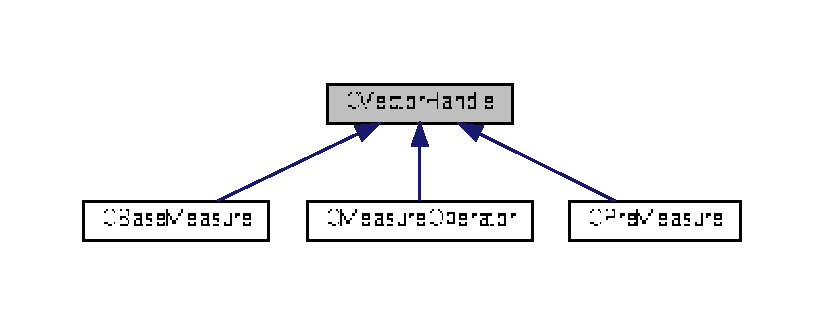
\includegraphics[width=350pt]{d7/d40/classCVectorHandle__inherit__graph}
\end{center}
\end{figure}
\subsection*{Public Member Functions}
\begin{DoxyCompactItemize}
\item 
\hyperlink{classCVectorHandle_ac6b74f660515541066f809b1339b2fdd}{C\+Vector\+Handle} ()
\begin{DoxyCompactList}\small\item\em does nothing \end{DoxyCompactList}\item 
\hyperlink{classCVectorHandle_a74e5aee7e24867695dafa409ab39a379}{$\sim$\+C\+Vector\+Handle} ()
\begin{DoxyCompactList}\small\item\em destructor\+: calls C\+Vector\+Handle\+::\+\_\+\+De\+Init() \end{DoxyCompactList}\item 
int \hyperlink{classCVectorHandle_ab1c2a8cb7d2f87077c6be60a86e2ae16}{Get\+Index\+By\+Short\+Label} (const string \&str\+Short\+Label)
\begin{DoxyCompactList}\small\item\em returns the index of the pre-\/unit if the user given string matches one of the elemens in C\+Pre\+Unit\+::m\+\_\+vstr\+Pre\+Unit\+Short \end{DoxyCompactList}\item 
int \hyperlink{classCVectorHandle_a36419c6f77002dde25bfa9e43357bd5c}{Get\+Index\+By\+Long\+Label} (const string \&str\+Long\+Label)
\begin{DoxyCompactList}\small\item\em returns the index of the pre-\/unit if the user given string matches one of the elemens in C\+Pre\+Unit\+::m\+\_\+vstr\+Pre\+Unit\+Long \end{DoxyCompactList}\item 
const string \& \hyperlink{classCVectorHandle_a392678513c7224a67022720797ac7b1b}{Long} (const unsigned int ui\+Index)
\begin{DoxyCompactList}\small\item\em gets element from \hyperlink{classCVectorHandle_afb50c8a33d4cf70bf92c644dca409ea2}{C\+Vector\+Handle\+::vstr\+Short} by index \end{DoxyCompactList}\item 
const string \& \hyperlink{classCVectorHandle_ac26fa8d3b66a5cc88dea0b411f5e20de}{Short} (const unsigned int ui\+Index)
\begin{DoxyCompactList}\small\item\em gets element from \hyperlink{classCVectorHandle_a71bec0e385b9ca8e5ffa174b559da9f8}{C\+Vector\+Handle\+::vstr\+Long} by index \end{DoxyCompactList}\item 
const double \hyperlink{classCVectorHandle_ae07ef54ee4ecb2da32176e58cf852e7c}{Factor} (const unsigned int ui\+Index)
\begin{DoxyCompactList}\small\item\em gets element from \hyperlink{classCVectorHandle_af8f8b2e0da8363e695872ca85f33364e}{C\+Vector\+Handle\+::vd\+Factor} by index \end{DoxyCompactList}\end{DoxyCompactItemize}
\subsection*{Protected Attributes}
\begin{DoxyCompactItemize}
\item 
vector$<$ double $>$ $\ast$ \hyperlink{classCVectorHandle_af8f8b2e0da8363e695872ca85f33364e}{vd\+Factor}
\begin{DoxyCompactList}\small\item\em vector keeping all the factors\+:~\newline
 e.\+g. \end{DoxyCompactList}\item 
vector$<$ string $>$ $\ast$ \hyperlink{classCVectorHandle_a71bec0e385b9ca8e5ffa174b559da9f8}{vstr\+Long}
\begin{DoxyCompactList}\small\item\em vector keeping the long label~\newline
 e.\+g. \end{DoxyCompactList}\item 
vector$<$ string $>$ $\ast$ \hyperlink{classCVectorHandle_afb50c8a33d4cf70bf92c644dca409ea2}{vstr\+Short}
\begin{DoxyCompactList}\small\item\em vector keeping the short label\+:~\newline
 e.\+g. \end{DoxyCompactList}\end{DoxyCompactItemize}


\subsection{Detailed Description}
This class keeps three vectors (two string \+: Short and Long and one double \+: Factor). These vectors are common to classes \hyperlink{classCPreMeasure}{C\+Pre\+Measure} and \hyperlink{classCBaseMeasure}{C\+Base\+Measure} and are therefore packed into this class for vector handling. 

Definition at line 37 of file Vector\+Handle.\+h.



\subsection{Constructor \& Destructor Documentation}
\mbox{\Hypertarget{classCVectorHandle_ac6b74f660515541066f809b1339b2fdd}\label{classCVectorHandle_ac6b74f660515541066f809b1339b2fdd}} 
\index{C\+Vector\+Handle@{C\+Vector\+Handle}!C\+Vector\+Handle@{C\+Vector\+Handle}}
\index{C\+Vector\+Handle@{C\+Vector\+Handle}!C\+Vector\+Handle@{C\+Vector\+Handle}}
\subsubsection{\texorpdfstring{C\+Vector\+Handle()}{CVectorHandle()}}
{\footnotesize\ttfamily C\+Vector\+Handle\+::\+C\+Vector\+Handle (\begin{DoxyParamCaption}{ }\end{DoxyParamCaption})}



does nothing 



Definition at line 28 of file Vector\+Handle.\+cpp.



References vd\+Factor, vstr\+Long, and vstr\+Short.

\mbox{\Hypertarget{classCVectorHandle_a74e5aee7e24867695dafa409ab39a379}\label{classCVectorHandle_a74e5aee7e24867695dafa409ab39a379}} 
\index{C\+Vector\+Handle@{C\+Vector\+Handle}!````~C\+Vector\+Handle@{$\sim$\+C\+Vector\+Handle}}
\index{````~C\+Vector\+Handle@{$\sim$\+C\+Vector\+Handle}!C\+Vector\+Handle@{C\+Vector\+Handle}}
\subsubsection{\texorpdfstring{$\sim$\+C\+Vector\+Handle()}{~CVectorHandle()}}
{\footnotesize\ttfamily C\+Vector\+Handle\+::$\sim$\+C\+Vector\+Handle (\begin{DoxyParamCaption}{ }\end{DoxyParamCaption})}



destructor\+: calls C\+Vector\+Handle\+::\+\_\+\+De\+Init() 



Definition at line 36 of file Vector\+Handle.\+cpp.



References Secure\+Delete\+Object\+Pointer(), vd\+Factor, vstr\+Long, and vstr\+Short.



\subsection{Member Function Documentation}
\mbox{\Hypertarget{classCVectorHandle_ae07ef54ee4ecb2da32176e58cf852e7c}\label{classCVectorHandle_ae07ef54ee4ecb2da32176e58cf852e7c}} 
\index{C\+Vector\+Handle@{C\+Vector\+Handle}!Factor@{Factor}}
\index{Factor@{Factor}!C\+Vector\+Handle@{C\+Vector\+Handle}}
\subsubsection{\texorpdfstring{Factor()}{Factor()}}
{\footnotesize\ttfamily const double C\+Vector\+Handle\+::\+Factor (\begin{DoxyParamCaption}\item[{const unsigned int}]{ui\+Index }\end{DoxyParamCaption})\hspace{0.3cm}{\ttfamily [inline]}}



gets element from \hyperlink{classCVectorHandle_af8f8b2e0da8363e695872ca85f33364e}{C\+Vector\+Handle\+::vd\+Factor} by index 


\begin{DoxyParams}{Parameters}
{\em ui\+Index} & index \\
\hline
\end{DoxyParams}
\begin{DoxyReturn}{Returns}
double\+: factor 
\end{DoxyReturn}


Definition at line 116 of file Vector\+Handle.\+h.



References Get\+Element\+From\+Vector\+By\+Index().

\mbox{\Hypertarget{classCVectorHandle_a36419c6f77002dde25bfa9e43357bd5c}\label{classCVectorHandle_a36419c6f77002dde25bfa9e43357bd5c}} 
\index{C\+Vector\+Handle@{C\+Vector\+Handle}!Get\+Index\+By\+Long\+Label@{Get\+Index\+By\+Long\+Label}}
\index{Get\+Index\+By\+Long\+Label@{Get\+Index\+By\+Long\+Label}!C\+Vector\+Handle@{C\+Vector\+Handle}}
\subsubsection{\texorpdfstring{Get\+Index\+By\+Long\+Label()}{GetIndexByLongLabel()}}
{\footnotesize\ttfamily int C\+Vector\+Handle\+::\+Get\+Index\+By\+Long\+Label (\begin{DoxyParamCaption}\item[{const string \&}]{str\+Long\+Label }\end{DoxyParamCaption})\hspace{0.3cm}{\ttfamily [inline]}}



returns the index of the pre-\/unit if the user given string matches one of the elemens in C\+Pre\+Unit\+::m\+\_\+vstr\+Pre\+Unit\+Long 


\begin{DoxyParams}{Parameters}
{\em str\+Long\+Label} & p\+\_\+str\+Pre\+Unit\+Long\+Label\+: user given long label of the demanded unit \\
\hline
\end{DoxyParams}
\begin{DoxyReturn}{Returns}
const unsigned int\& 
\end{DoxyReturn}


Definition at line 80 of file Vector\+Handle.\+h.



References Find\+Element\+In\+Vector\+Get\+Index().

\mbox{\Hypertarget{classCVectorHandle_ab1c2a8cb7d2f87077c6be60a86e2ae16}\label{classCVectorHandle_ab1c2a8cb7d2f87077c6be60a86e2ae16}} 
\index{C\+Vector\+Handle@{C\+Vector\+Handle}!Get\+Index\+By\+Short\+Label@{Get\+Index\+By\+Short\+Label}}
\index{Get\+Index\+By\+Short\+Label@{Get\+Index\+By\+Short\+Label}!C\+Vector\+Handle@{C\+Vector\+Handle}}
\subsubsection{\texorpdfstring{Get\+Index\+By\+Short\+Label()}{GetIndexByShortLabel()}}
{\footnotesize\ttfamily int C\+Vector\+Handle\+::\+Get\+Index\+By\+Short\+Label (\begin{DoxyParamCaption}\item[{const string \&}]{str\+Short\+Label }\end{DoxyParamCaption})\hspace{0.3cm}{\ttfamily [inline]}}



returns the index of the pre-\/unit if the user given string matches one of the elemens in C\+Pre\+Unit\+::m\+\_\+vstr\+Pre\+Unit\+Short 


\begin{DoxyParams}{Parameters}
{\em str\+Short\+Label} & p\+\_\+str\+Pre\+Unit\+Short\+Label\+:user given short label of the demanded unit \\
\hline
\end{DoxyParams}
\begin{DoxyReturn}{Returns}
const unsigned int\& 
\end{DoxyReturn}


Definition at line 69 of file Vector\+Handle.\+h.



References Find\+Element\+In\+Vector\+Get\+Index().

\mbox{\Hypertarget{classCVectorHandle_a392678513c7224a67022720797ac7b1b}\label{classCVectorHandle_a392678513c7224a67022720797ac7b1b}} 
\index{C\+Vector\+Handle@{C\+Vector\+Handle}!Long@{Long}}
\index{Long@{Long}!C\+Vector\+Handle@{C\+Vector\+Handle}}
\subsubsection{\texorpdfstring{Long()}{Long()}}
{\footnotesize\ttfamily const string\& C\+Vector\+Handle\+::\+Long (\begin{DoxyParamCaption}\item[{const unsigned int}]{ui\+Index }\end{DoxyParamCaption})\hspace{0.3cm}{\ttfamily [inline]}}



gets element from \hyperlink{classCVectorHandle_afb50c8a33d4cf70bf92c644dca409ea2}{C\+Vector\+Handle\+::vstr\+Short} by index 


\begin{DoxyParams}{Parameters}
{\em ui\+Index} & index \\
\hline
\end{DoxyParams}
\begin{DoxyReturn}{Returns}
string\+: long label 
\end{DoxyReturn}


Definition at line 94 of file Vector\+Handle.\+h.



References Get\+Element\+From\+Vector\+By\+Index().

\mbox{\Hypertarget{classCVectorHandle_ac26fa8d3b66a5cc88dea0b411f5e20de}\label{classCVectorHandle_ac26fa8d3b66a5cc88dea0b411f5e20de}} 
\index{C\+Vector\+Handle@{C\+Vector\+Handle}!Short@{Short}}
\index{Short@{Short}!C\+Vector\+Handle@{C\+Vector\+Handle}}
\subsubsection{\texorpdfstring{Short()}{Short()}}
{\footnotesize\ttfamily const string\& C\+Vector\+Handle\+::\+Short (\begin{DoxyParamCaption}\item[{const unsigned int}]{ui\+Index }\end{DoxyParamCaption})\hspace{0.3cm}{\ttfamily [inline]}}



gets element from \hyperlink{classCVectorHandle_a71bec0e385b9ca8e5ffa174b559da9f8}{C\+Vector\+Handle\+::vstr\+Long} by index 


\begin{DoxyParams}{Parameters}
{\em ui\+Index} & index \\
\hline
\end{DoxyParams}
\begin{DoxyReturn}{Returns}
string\+: short label 
\end{DoxyReturn}


Definition at line 105 of file Vector\+Handle.\+h.



References Get\+Element\+From\+Vector\+By\+Index().



\subsection{Member Data Documentation}
\mbox{\Hypertarget{classCVectorHandle_af8f8b2e0da8363e695872ca85f33364e}\label{classCVectorHandle_af8f8b2e0da8363e695872ca85f33364e}} 
\index{C\+Vector\+Handle@{C\+Vector\+Handle}!vd\+Factor@{vd\+Factor}}
\index{vd\+Factor@{vd\+Factor}!C\+Vector\+Handle@{C\+Vector\+Handle}}
\subsubsection{\texorpdfstring{vd\+Factor}{vdFactor}}
{\footnotesize\ttfamily vector$<$double$>$$\ast$ C\+Vector\+Handle\+::vd\+Factor\hspace{0.3cm}{\ttfamily [protected]}}



vector keeping all the factors\+:~\newline
 e.\+g. 


\begin{DoxyItemize}
\item \hyperlink{classCPreMeasure}{C\+Pre\+Measure}\+: milli --$>$ 0.\+001
\item \hyperlink{classCBaseMeasure}{C\+Base\+Measure}\+: °F --$>$ 5/9 (SI recalculation factor for °K) 
\end{DoxyItemize}

Definition at line 136 of file Vector\+Handle.\+h.

\mbox{\Hypertarget{classCVectorHandle_a71bec0e385b9ca8e5ffa174b559da9f8}\label{classCVectorHandle_a71bec0e385b9ca8e5ffa174b559da9f8}} 
\index{C\+Vector\+Handle@{C\+Vector\+Handle}!vstr\+Long@{vstr\+Long}}
\index{vstr\+Long@{vstr\+Long}!C\+Vector\+Handle@{C\+Vector\+Handle}}
\subsubsection{\texorpdfstring{vstr\+Long}{vstrLong}}
{\footnotesize\ttfamily vector$<$string$>$$\ast$ C\+Vector\+Handle\+::vstr\+Long\hspace{0.3cm}{\ttfamily [protected]}}



vector keeping the long label~\newline
 e.\+g. 


\begin{DoxyItemize}
\item \hyperlink{classCPreMeasure}{C\+Pre\+Measure}\+: milli --$>$ \char`\"{}milli\char`\"{}
\item \hyperlink{classCBaseMeasure}{C\+Base\+Measure}\+: volt --$>$ \char`\"{}volt\char`\"{} 
\end{DoxyItemize}

Definition at line 145 of file Vector\+Handle.\+h.

\mbox{\Hypertarget{classCVectorHandle_afb50c8a33d4cf70bf92c644dca409ea2}\label{classCVectorHandle_afb50c8a33d4cf70bf92c644dca409ea2}} 
\index{C\+Vector\+Handle@{C\+Vector\+Handle}!vstr\+Short@{vstr\+Short}}
\index{vstr\+Short@{vstr\+Short}!C\+Vector\+Handle@{C\+Vector\+Handle}}
\subsubsection{\texorpdfstring{vstr\+Short}{vstrShort}}
{\footnotesize\ttfamily vector$<$string$>$$\ast$ C\+Vector\+Handle\+::vstr\+Short\hspace{0.3cm}{\ttfamily [protected]}}



vector keeping the short label\+:~\newline
 e.\+g. 


\begin{DoxyItemize}
\item \hyperlink{classCPreMeasure}{C\+Pre\+Measure}\+: milli --$>$ \char`\"{}m\char`\"{}
\item \hyperlink{classCBaseMeasure}{C\+Base\+Measure}\+: volt --$>$ \char`\"{}\+V\char`\"{} 
\end{DoxyItemize}

Definition at line 154 of file Vector\+Handle.\+h.



The documentation for this class was generated from the following files\+:\begin{DoxyCompactItemize}
\item 
Floating\+Measure/\+Measure/\hyperlink{VectorHandle_8h}{Vector\+Handle.\+h}\item 
Floating\+Measure/\+Measure/\hyperlink{VectorHandle_8cpp}{Vector\+Handle.\+cpp}\end{DoxyCompactItemize}

\hypertarget{uniondbl__64}{}\section{dbl\+\_\+64 Union Reference}
\label{uniondbl__64}\index{dbl\+\_\+64@{dbl\+\_\+64}}


union for calculation of numerical error of a 64 bit double  




{\ttfamily \#include $<$Utils.\+h$>$}

\subsection*{Public Attributes}
\begin{DoxyCompactItemize}
\item 
long long \hyperlink{uniondbl__64_a6f97524990aa26aaa1618b7288301841}{i64}
\begin{DoxyCompactList}\small\item\em 64 bit integer representation \end{DoxyCompactList}\item 
double \hyperlink{uniondbl__64_a6007036e300f1924037fc32c8bec660c}{d64}
\begin{DoxyCompactList}\small\item\em 64 bit double representation \end{DoxyCompactList}\end{DoxyCompactItemize}


\subsection{Detailed Description}
union for calculation of numerical error of a 64 bit double 

Definition at line 79 of file Utils.\+h.



\subsection{Member Data Documentation}
\mbox{\Hypertarget{uniondbl__64_a6007036e300f1924037fc32c8bec660c}\label{uniondbl__64_a6007036e300f1924037fc32c8bec660c}} 
\index{dbl\+\_\+64@{dbl\+\_\+64}!d64@{d64}}
\index{d64@{d64}!dbl\+\_\+64@{dbl\+\_\+64}}
\subsubsection{\texorpdfstring{d64}{d64}}
{\footnotesize\ttfamily double dbl\+\_\+64\+::d64}



64 bit double representation 



Definition at line 89 of file Utils.\+h.

\mbox{\Hypertarget{uniondbl__64_a6f97524990aa26aaa1618b7288301841}\label{uniondbl__64_a6f97524990aa26aaa1618b7288301841}} 
\index{dbl\+\_\+64@{dbl\+\_\+64}!i64@{i64}}
\index{i64@{i64}!dbl\+\_\+64@{dbl\+\_\+64}}
\subsubsection{\texorpdfstring{i64}{i64}}
{\footnotesize\ttfamily long long dbl\+\_\+64\+::i64}



64 bit integer representation 



Definition at line 84 of file Utils.\+h.



The documentation for this union was generated from the following file\+:\begin{DoxyCompactItemize}
\item 
Floating\+Measure/\+Utils/\hyperlink{Utils_8h}{Utils.\+h}\end{DoxyCompactItemize}

\chapter{File Documentation}
\hypertarget{DigFloat_8cpp}{}\section{Floating\+Measure/\+Dig\+Float/\+Dig\+Float.cpp File Reference}
\label{DigFloat_8cpp}\index{Floating\+Measure/\+Dig\+Float/\+Dig\+Float.\+cpp@{Floating\+Measure/\+Dig\+Float/\+Dig\+Float.\+cpp}}
{\ttfamily \#include \char`\"{}Dig\+Float.\+h\char`\"{}}\newline
{\ttfamily \#include $<$iostream$>$}\newline
Include dependency graph for Dig\+Float.\+cpp\+:\nopagebreak
\begin{figure}[H]
\begin{center}
\leavevmode
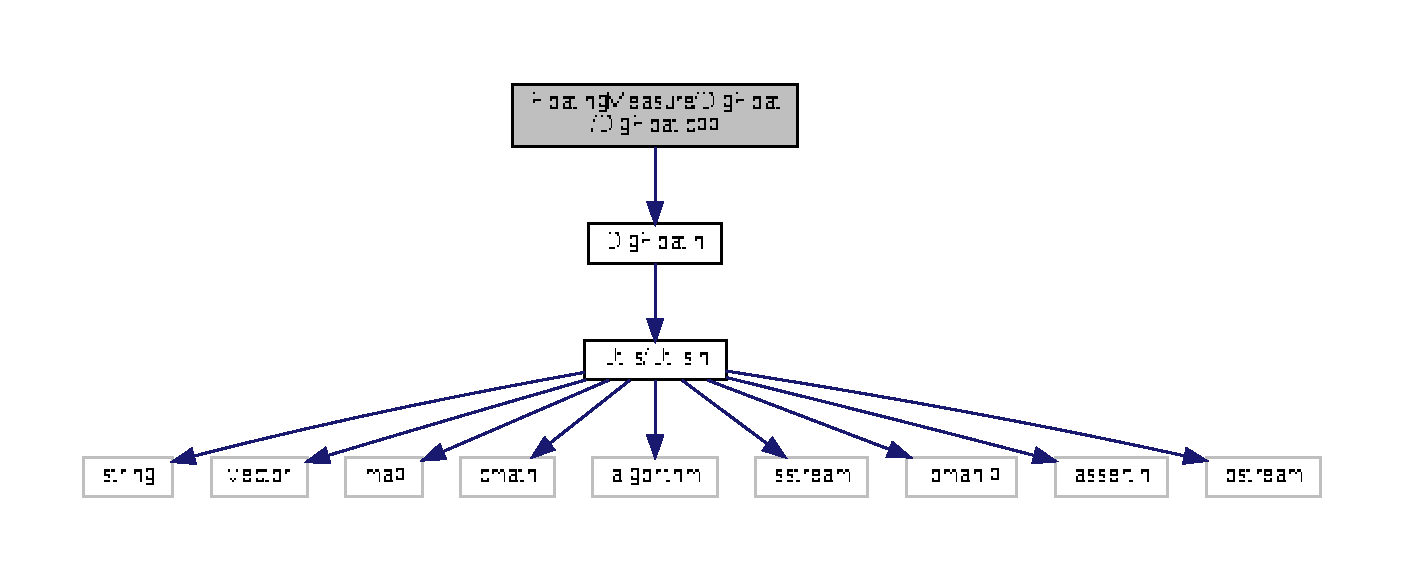
\includegraphics[width=350pt]{dc/da8/DigFloat_8cpp__incl}
\end{center}
\end{figure}
\subsection*{Functions}
\begin{DoxyCompactItemize}
\item 
\hyperlink{classCDigFloat}{C\+Dig\+Float} \hyperlink{DigFloat_8cpp_a269b310d675c311c6e0894bf326593ae}{abs} (const \hyperlink{classCDigFloat}{C\+Dig\+Float} \&DF)
\begin{DoxyCompactList}\small\item\em abs\+: returns \hyperlink{classCDigFloat}{C\+Dig\+Float} with absolute value; \end{DoxyCompactList}\item 
\hyperlink{classCDigFloat}{C\+Dig\+Float} \hyperlink{DigFloat_8cpp_a25031604af1e6356848a9ac84c209903}{log} (const \hyperlink{classCDigFloat}{C\+Dig\+Float} \&DF, const \hyperlink{classCDigFloat}{C\+Dig\+Float} \&df\+Base)
\begin{DoxyCompactList}\small\item\em log\+: returns \hyperlink{classCDigFloat}{C\+Dig\+Float} logarithm to user given base (default\+: natural logarithm with base euler number); \end{DoxyCompactList}\item 
\hyperlink{classCDigFloat}{C\+Dig\+Float} \hyperlink{DigFloat_8cpp_ac5877d13039d236858e1cb04351f0a86}{pow} (const \hyperlink{classCDigFloat}{C\+Dig\+Float} \&df\+Base, const \hyperlink{classCDigFloat}{C\+Dig\+Float} \&df\+Exp)
\begin{DoxyCompactList}\small\item\em pow\+: returns \hyperlink{classCDigFloat}{C\+Dig\+Float} exponential expression to user given base and exponent \end{DoxyCompactList}\item 
\hyperlink{classCDigFloat}{C\+Dig\+Float} \hyperlink{DigFloat_8cpp_a2206715f4b83afeea6339373bb3631fb}{exp} (const \hyperlink{classCDigFloat}{C\+Dig\+Float} \&df\+Exp)
\begin{DoxyCompactList}\small\item\em exp\+: returns \hyperlink{classCDigFloat}{C\+Dig\+Float} exponential expression to Euler number and user given exponent \end{DoxyCompactList}\item 
\hyperlink{classCDigFloat}{C\+Dig\+Float} \hyperlink{DigFloat_8cpp_ae66acb4f3bea83a9fad22cc58fe50905}{sqrt} (const \hyperlink{classCDigFloat}{C\+Dig\+Float} \&DF)
\begin{DoxyCompactList}\small\item\em sqrt\+: returns \hyperlink{classCDigFloat}{C\+Dig\+Float} as square root of user given value \end{DoxyCompactList}\item 
\hyperlink{classCDigFloat}{C\+Dig\+Float} \hyperlink{DigFloat_8cpp_a4362c8e7ae2a6d36f84b278d4a915a61}{max} (const \hyperlink{classCDigFloat}{C\+Dig\+Float} \&one, const \hyperlink{classCDigFloat}{C\+Dig\+Float} \&other)
\begin{DoxyCompactList}\small\item\em max\+: returns the greater \hyperlink{classCDigFloat}{C\+Dig\+Float} \end{DoxyCompactList}\item 
\hyperlink{classCDigFloat}{C\+Dig\+Float} \hyperlink{DigFloat_8cpp_aa52baf47e5c050a2d10794b2e460948d}{min} (const \hyperlink{classCDigFloat}{C\+Dig\+Float} \&one, const \hyperlink{classCDigFloat}{C\+Dig\+Float} \&other)
\begin{DoxyCompactList}\small\item\em min\+: returns the smaller \hyperlink{classCDigFloat}{C\+Dig\+Float} \end{DoxyCompactList}\item 
\hyperlink{classCDigFloat}{C\+Dig\+Float} \hyperlink{DigFloat_8cpp_a884d892dc5da6c1e8aacafbe6338d740}{operator+} (const \hyperlink{classCDigFloat}{C\+Dig\+Float} \&One, const \hyperlink{classCDigFloat}{C\+Dig\+Float} \&Other)
\begin{DoxyCompactList}\small\item\em operator+ \end{DoxyCompactList}\item 
\hyperlink{classCDigFloat}{C\+Dig\+Float} \hyperlink{DigFloat_8cpp_a6155f32f19e3616df05adc16049042a4}{operator-\/} (const \hyperlink{classCDigFloat}{C\+Dig\+Float} \&One)
\begin{DoxyCompactList}\small\item\em operator-\/ for expression \char`\"{}-\/\+X\char`\"{} instead of X$\ast$(-\/1) \end{DoxyCompactList}\item 
\hyperlink{classCDigFloat}{C\+Dig\+Float} \hyperlink{DigFloat_8cpp_abf4279bd474679b4ecfc24124d246af1}{operator-\/} (const \hyperlink{classCDigFloat}{C\+Dig\+Float} \&One, const \hyperlink{classCDigFloat}{C\+Dig\+Float} \&Other)
\begin{DoxyCompactList}\small\item\em operator-\/ \end{DoxyCompactList}\item 
\hyperlink{classCDigFloat}{C\+Dig\+Float} \hyperlink{DigFloat_8cpp_a4f045c1be909c3a6dadee063c4f854c3}{operator$\ast$} (const \hyperlink{classCDigFloat}{C\+Dig\+Float} \&One, const \hyperlink{classCDigFloat}{C\+Dig\+Float} \&Other)
\begin{DoxyCompactList}\small\item\em operator$\ast$ \end{DoxyCompactList}\item 
\hyperlink{classCDigFloat}{C\+Dig\+Float} \hyperlink{DigFloat_8cpp_ae7276c529ed6a82015d5114b6c4c392f}{operator/} (const \hyperlink{classCDigFloat}{C\+Dig\+Float} \&One, const \hyperlink{classCDigFloat}{C\+Dig\+Float} \&Other)
\begin{DoxyCompactList}\small\item\em operator/ \end{DoxyCompactList}\end{DoxyCompactItemize}


\subsection{Function Documentation}
\mbox{\Hypertarget{DigFloat_8cpp_a269b310d675c311c6e0894bf326593ae}\label{DigFloat_8cpp_a269b310d675c311c6e0894bf326593ae}} 
\index{Dig\+Float.\+cpp@{Dig\+Float.\+cpp}!abs@{abs}}
\index{abs@{abs}!Dig\+Float.\+cpp@{Dig\+Float.\+cpp}}
\subsubsection{\texorpdfstring{abs()}{abs()}}
{\footnotesize\ttfamily \hyperlink{classCDigFloat}{C\+Dig\+Float} abs (\begin{DoxyParamCaption}\item[{const \hyperlink{classCDigFloat}{C\+Dig\+Float} \&}]{DF }\end{DoxyParamCaption})}



abs\+: returns \hyperlink{classCDigFloat}{C\+Dig\+Float} with absolute value; 


\begin{DoxyParams}{Parameters}
{\em FM} & \hyperlink{classCDigFloat}{C\+Dig\+Float} \\
\hline
\end{DoxyParams}
\begin{DoxyReturn}{Returns}
\hyperlink{classCDigFloat}{C\+Dig\+Float} 
\end{DoxyReturn}


Definition at line 302 of file Dig\+Float.\+cpp.



References C\+Dig\+Float\+::\+Raw\+Value().

\mbox{\Hypertarget{DigFloat_8cpp_a2206715f4b83afeea6339373bb3631fb}\label{DigFloat_8cpp_a2206715f4b83afeea6339373bb3631fb}} 
\index{Dig\+Float.\+cpp@{Dig\+Float.\+cpp}!exp@{exp}}
\index{exp@{exp}!Dig\+Float.\+cpp@{Dig\+Float.\+cpp}}
\subsubsection{\texorpdfstring{exp()}{exp()}}
{\footnotesize\ttfamily \hyperlink{classCDigFloat}{C\+Dig\+Float} exp (\begin{DoxyParamCaption}\item[{const \hyperlink{classCDigFloat}{C\+Dig\+Float} \&}]{df\+Exp }\end{DoxyParamCaption})}



exp\+: returns \hyperlink{classCDigFloat}{C\+Dig\+Float} exponential expression to Euler number and user given exponent 


\begin{DoxyParams}{Parameters}
{\em df\+Exp} & \hyperlink{classCDigFloat}{C\+Dig\+Float} as exponent \\
\hline
\end{DoxyParams}
\begin{DoxyReturn}{Returns}
\hyperlink{classCDigFloat}{C\+Dig\+Float} 
\end{DoxyReturn}


Definition at line 392 of file Dig\+Float.\+cpp.



References C\+Dig\+Float\+::d\+Error, C\+Dig\+Float\+::exp, C\+Dig\+Float\+::\+Raw\+Error(), C\+Dig\+Float\+::\+Raw\+Value(), C\+Dig\+Float\+::\+Value\+Max\+Limit(), and C\+Dig\+Float\+::\+Value\+Min\+Limit().

\mbox{\Hypertarget{DigFloat_8cpp_a25031604af1e6356848a9ac84c209903}\label{DigFloat_8cpp_a25031604af1e6356848a9ac84c209903}} 
\index{Dig\+Float.\+cpp@{Dig\+Float.\+cpp}!log@{log}}
\index{log@{log}!Dig\+Float.\+cpp@{Dig\+Float.\+cpp}}
\subsubsection{\texorpdfstring{log()}{log()}}
{\footnotesize\ttfamily \hyperlink{classCDigFloat}{C\+Dig\+Float} log (\begin{DoxyParamCaption}\item[{const \hyperlink{classCDigFloat}{C\+Dig\+Float} \&}]{DF,  }\item[{const \hyperlink{classCDigFloat}{C\+Dig\+Float} \&}]{df\+Base = {\ttfamily 0} }\end{DoxyParamCaption})}



log\+: returns \hyperlink{classCDigFloat}{C\+Dig\+Float} logarithm to user given base (default\+: natural logarithm with base euler number); 


\begin{DoxyParams}{Parameters}
{\em DF} & \hyperlink{classCDigFloat}{C\+Dig\+Float} \\
\hline
{\em df\+Base} & \hyperlink{classCDigFloat}{C\+Dig\+Float} as base (optional) \\
\hline
\end{DoxyParams}
\begin{DoxyReturn}{Returns}
\hyperlink{classCDigFloat}{C\+Dig\+Float} 
\end{DoxyReturn}


Definition at line 309 of file Dig\+Float.\+cpp.



References C\+Dig\+Float\+::d\+Error, C\+Dig\+Float\+::\+Error(), C\+Dig\+Float\+::\+Raw\+Error(), C\+Dig\+Float\+::\+Raw\+Value(), C\+Dig\+Float\+::\+Value\+Max\+Limit(), and C\+Dig\+Float\+::\+Value\+Min\+Limit().

\mbox{\Hypertarget{DigFloat_8cpp_a4362c8e7ae2a6d36f84b278d4a915a61}\label{DigFloat_8cpp_a4362c8e7ae2a6d36f84b278d4a915a61}} 
\index{Dig\+Float.\+cpp@{Dig\+Float.\+cpp}!max@{max}}
\index{max@{max}!Dig\+Float.\+cpp@{Dig\+Float.\+cpp}}
\subsubsection{\texorpdfstring{max()}{max()}}
{\footnotesize\ttfamily \hyperlink{classCDigFloat}{C\+Dig\+Float} max (\begin{DoxyParamCaption}\item[{const \hyperlink{classCDigFloat}{C\+Dig\+Float} \&}]{one,  }\item[{const \hyperlink{classCDigFloat}{C\+Dig\+Float} \&}]{other }\end{DoxyParamCaption})}



max\+: returns the greater \hyperlink{classCDigFloat}{C\+Dig\+Float} 


\begin{DoxyParams}{Parameters}
{\em one} & \hyperlink{classCDigFloat}{C\+Dig\+Float} to compare with other \\
\hline
{\em other} & \hyperlink{classCDigFloat}{C\+Dig\+Float} to compare with one \\
\hline
\end{DoxyParams}
\begin{DoxyReturn}{Returns}
\hyperlink{classCDigFloat}{C\+Dig\+Float} (one or the other) 
\end{DoxyReturn}


Definition at line 427 of file Dig\+Float.\+cpp.

\mbox{\Hypertarget{DigFloat_8cpp_aa52baf47e5c050a2d10794b2e460948d}\label{DigFloat_8cpp_aa52baf47e5c050a2d10794b2e460948d}} 
\index{Dig\+Float.\+cpp@{Dig\+Float.\+cpp}!min@{min}}
\index{min@{min}!Dig\+Float.\+cpp@{Dig\+Float.\+cpp}}
\subsubsection{\texorpdfstring{min()}{min()}}
{\footnotesize\ttfamily \hyperlink{classCDigFloat}{C\+Dig\+Float} min (\begin{DoxyParamCaption}\item[{const \hyperlink{classCDigFloat}{C\+Dig\+Float} \&}]{one,  }\item[{const \hyperlink{classCDigFloat}{C\+Dig\+Float} \&}]{other }\end{DoxyParamCaption})}



min\+: returns the smaller \hyperlink{classCDigFloat}{C\+Dig\+Float} 


\begin{DoxyParams}{Parameters}
{\em one} & \hyperlink{classCDigFloat}{C\+Dig\+Float} to compare with other \\
\hline
{\em other} & \hyperlink{classCDigFloat}{C\+Dig\+Float} to compare with one \\
\hline
\end{DoxyParams}
\begin{DoxyReturn}{Returns}
\hyperlink{classCDigFloat}{C\+Dig\+Float} (one or the other) 
\end{DoxyReturn}


Definition at line 436 of file Dig\+Float.\+cpp.

\mbox{\Hypertarget{DigFloat_8cpp_a4f045c1be909c3a6dadee063c4f854c3}\label{DigFloat_8cpp_a4f045c1be909c3a6dadee063c4f854c3}} 
\index{Dig\+Float.\+cpp@{Dig\+Float.\+cpp}!operator$\ast$@{operator$\ast$}}
\index{operator$\ast$@{operator$\ast$}!Dig\+Float.\+cpp@{Dig\+Float.\+cpp}}
\subsubsection{\texorpdfstring{operator$\ast$()}{operator*()}}
{\footnotesize\ttfamily \hyperlink{classCDigFloat}{C\+Dig\+Float} operator$\ast$ (\begin{DoxyParamCaption}\item[{const \hyperlink{classCDigFloat}{C\+Dig\+Float} \&}]{One,  }\item[{const \hyperlink{classCDigFloat}{C\+Dig\+Float} \&}]{Other }\end{DoxyParamCaption})}



operator$\ast$ 


\begin{DoxyParams}{Parameters}
{\em One} & \hyperlink{classCDigFloat}{C\+Dig\+Float} \\
\hline
{\em Other} & \hyperlink{classCDigFloat}{C\+Dig\+Float} \\
\hline
\end{DoxyParams}
\begin{DoxyReturn}{Returns}
\hyperlink{classCDigFloat}{C\+Dig\+Float} 
\end{DoxyReturn}


Definition at line 464 of file Dig\+Float.\+cpp.

\mbox{\Hypertarget{DigFloat_8cpp_a884d892dc5da6c1e8aacafbe6338d740}\label{DigFloat_8cpp_a884d892dc5da6c1e8aacafbe6338d740}} 
\index{Dig\+Float.\+cpp@{Dig\+Float.\+cpp}!operator+@{operator+}}
\index{operator+@{operator+}!Dig\+Float.\+cpp@{Dig\+Float.\+cpp}}
\subsubsection{\texorpdfstring{operator+()}{operator+()}}
{\footnotesize\ttfamily \hyperlink{classCDigFloat}{C\+Dig\+Float} operator+ (\begin{DoxyParamCaption}\item[{const \hyperlink{classCDigFloat}{C\+Dig\+Float} \&}]{One,  }\item[{const \hyperlink{classCDigFloat}{C\+Dig\+Float} \&}]{Other }\end{DoxyParamCaption})}



operator+ 


\begin{DoxyParams}{Parameters}
{\em One} & \hyperlink{classCDigFloat}{C\+Dig\+Float} \\
\hline
{\em Other} & \hyperlink{classCDigFloat}{C\+Dig\+Float} \\
\hline
\end{DoxyParams}
\begin{DoxyReturn}{Returns}
\hyperlink{classCDigFloat}{C\+Dig\+Float} 
\end{DoxyReturn}


Definition at line 444 of file Dig\+Float.\+cpp.

\mbox{\Hypertarget{DigFloat_8cpp_a6155f32f19e3616df05adc16049042a4}\label{DigFloat_8cpp_a6155f32f19e3616df05adc16049042a4}} 
\index{Dig\+Float.\+cpp@{Dig\+Float.\+cpp}!operator-\/@{operator-\/}}
\index{operator-\/@{operator-\/}!Dig\+Float.\+cpp@{Dig\+Float.\+cpp}}
\subsubsection{\texorpdfstring{operator-\/()}{operator-()}\hspace{0.1cm}{\footnotesize\ttfamily [1/2]}}
{\footnotesize\ttfamily \hyperlink{classCDigFloat}{C\+Dig\+Float} operator-\/ (\begin{DoxyParamCaption}\item[{const \hyperlink{classCDigFloat}{C\+Dig\+Float} \&}]{One }\end{DoxyParamCaption})}



operator-\/ for expression \char`\"{}-\/\+X\char`\"{} instead of X$\ast$(-\/1) 


\begin{DoxyParams}{Parameters}
{\em One} & \hyperlink{classCDigFloat}{C\+Dig\+Float} \\
\hline
{\em Other} & \hyperlink{classCDigFloat}{C\+Dig\+Float} \\
\hline
\end{DoxyParams}
\begin{DoxyReturn}{Returns}
\hyperlink{classCDigFloat}{C\+Dig\+Float} 
\end{DoxyReturn}


Definition at line 451 of file Dig\+Float.\+cpp.

\mbox{\Hypertarget{DigFloat_8cpp_abf4279bd474679b4ecfc24124d246af1}\label{DigFloat_8cpp_abf4279bd474679b4ecfc24124d246af1}} 
\index{Dig\+Float.\+cpp@{Dig\+Float.\+cpp}!operator-\/@{operator-\/}}
\index{operator-\/@{operator-\/}!Dig\+Float.\+cpp@{Dig\+Float.\+cpp}}
\subsubsection{\texorpdfstring{operator-\/()}{operator-()}\hspace{0.1cm}{\footnotesize\ttfamily [2/2]}}
{\footnotesize\ttfamily \hyperlink{classCDigFloat}{C\+Dig\+Float} operator-\/ (\begin{DoxyParamCaption}\item[{const \hyperlink{classCDigFloat}{C\+Dig\+Float} \&}]{One,  }\item[{const \hyperlink{classCDigFloat}{C\+Dig\+Float} \&}]{Other }\end{DoxyParamCaption})}



operator-\/ 


\begin{DoxyParams}{Parameters}
{\em One} & \hyperlink{classCDigFloat}{C\+Dig\+Float} \\
\hline
{\em Other} & \hyperlink{classCDigFloat}{C\+Dig\+Float} \\
\hline
\end{DoxyParams}
\begin{DoxyReturn}{Returns}
\hyperlink{classCDigFloat}{C\+Dig\+Float} 
\end{DoxyReturn}


Definition at line 456 of file Dig\+Float.\+cpp.

\mbox{\Hypertarget{DigFloat_8cpp_ae7276c529ed6a82015d5114b6c4c392f}\label{DigFloat_8cpp_ae7276c529ed6a82015d5114b6c4c392f}} 
\index{Dig\+Float.\+cpp@{Dig\+Float.\+cpp}!operator/@{operator/}}
\index{operator/@{operator/}!Dig\+Float.\+cpp@{Dig\+Float.\+cpp}}
\subsubsection{\texorpdfstring{operator/()}{operator/()}}
{\footnotesize\ttfamily \hyperlink{classCDigFloat}{C\+Dig\+Float} operator/ (\begin{DoxyParamCaption}\item[{const \hyperlink{classCDigFloat}{C\+Dig\+Float} \&}]{One,  }\item[{const \hyperlink{classCDigFloat}{C\+Dig\+Float} \&}]{Other }\end{DoxyParamCaption})}



operator/ 


\begin{DoxyParams}{Parameters}
{\em One} & \hyperlink{classCDigFloat}{C\+Dig\+Float} \\
\hline
{\em Other} & \hyperlink{classCDigFloat}{C\+Dig\+Float} \\
\hline
\end{DoxyParams}
\begin{DoxyReturn}{Returns}
\hyperlink{classCDigFloat}{C\+Dig\+Float} 
\end{DoxyReturn}


Definition at line 471 of file Dig\+Float.\+cpp.

\mbox{\Hypertarget{DigFloat_8cpp_ac5877d13039d236858e1cb04351f0a86}\label{DigFloat_8cpp_ac5877d13039d236858e1cb04351f0a86}} 
\index{Dig\+Float.\+cpp@{Dig\+Float.\+cpp}!pow@{pow}}
\index{pow@{pow}!Dig\+Float.\+cpp@{Dig\+Float.\+cpp}}
\subsubsection{\texorpdfstring{pow()}{pow()}}
{\footnotesize\ttfamily \hyperlink{classCDigFloat}{C\+Dig\+Float} pow (\begin{DoxyParamCaption}\item[{const \hyperlink{classCDigFloat}{C\+Dig\+Float} \&}]{df\+Base,  }\item[{const \hyperlink{classCDigFloat}{C\+Dig\+Float} \&}]{df\+Exp }\end{DoxyParamCaption})}



pow\+: returns \hyperlink{classCDigFloat}{C\+Dig\+Float} exponential expression to user given base and exponent 


\begin{DoxyParams}{Parameters}
{\em df\+Base} & \hyperlink{classCDigFloat}{C\+Dig\+Float} as base \\
\hline
{\em df\+Exp} & \hyperlink{classCDigFloat}{C\+Dig\+Float} as exponent \\
\hline
\end{DoxyParams}
\begin{DoxyReturn}{Returns}
\hyperlink{classCDigFloat}{C\+Dig\+Float} 
\end{DoxyReturn}


Definition at line 373 of file Dig\+Float.\+cpp.



References C\+Dig\+Float\+::d\+Error, max(), min(), C\+Dig\+Float\+::pow, C\+Dig\+Float\+::\+Raw\+Error(), C\+Dig\+Float\+::\+Raw\+Value(), C\+Dig\+Float\+::\+Value\+Max\+Limit(), and C\+Dig\+Float\+::\+Value\+Min\+Limit().

\mbox{\Hypertarget{DigFloat_8cpp_ae66acb4f3bea83a9fad22cc58fe50905}\label{DigFloat_8cpp_ae66acb4f3bea83a9fad22cc58fe50905}} 
\index{Dig\+Float.\+cpp@{Dig\+Float.\+cpp}!sqrt@{sqrt}}
\index{sqrt@{sqrt}!Dig\+Float.\+cpp@{Dig\+Float.\+cpp}}
\subsubsection{\texorpdfstring{sqrt()}{sqrt()}}
{\footnotesize\ttfamily \hyperlink{classCDigFloat}{C\+Dig\+Float} sqrt (\begin{DoxyParamCaption}\item[{const \hyperlink{classCDigFloat}{C\+Dig\+Float} \&}]{DF }\end{DoxyParamCaption})}



sqrt\+: returns \hyperlink{classCDigFloat}{C\+Dig\+Float} as square root of user given value 


\begin{DoxyParams}{Parameters}
{\em DF} & \hyperlink{classCDigFloat}{C\+Dig\+Float} \\
\hline
\end{DoxyParams}
\begin{DoxyReturn}{Returns}
\hyperlink{classCDigFloat}{C\+Dig\+Float} 
\end{DoxyReturn}


Definition at line 410 of file Dig\+Float.\+cpp.



References C\+Dig\+Float\+::d\+Error, C\+Dig\+Float\+::\+Raw\+Error(), C\+Dig\+Float\+::\+Raw\+Value(), C\+Dig\+Float\+::sqrt, C\+Dig\+Float\+::\+Value\+Max\+Limit(), and C\+Dig\+Float\+::\+Value\+Min\+Limit().


\hypertarget{DigFloat_8h}{}\section{Floating\+Measure/\+Dig\+Float/\+Dig\+Float.h File Reference}
\label{DigFloat_8h}\index{Floating\+Measure/\+Dig\+Float/\+Dig\+Float.\+h@{Floating\+Measure/\+Dig\+Float/\+Dig\+Float.\+h}}
{\ttfamily \#include $<$Utils/\+Utils.\+h$>$}\newline
Include dependency graph for Dig\+Float.\+h\+:\nopagebreak
\begin{figure}[H]
\begin{center}
\leavevmode
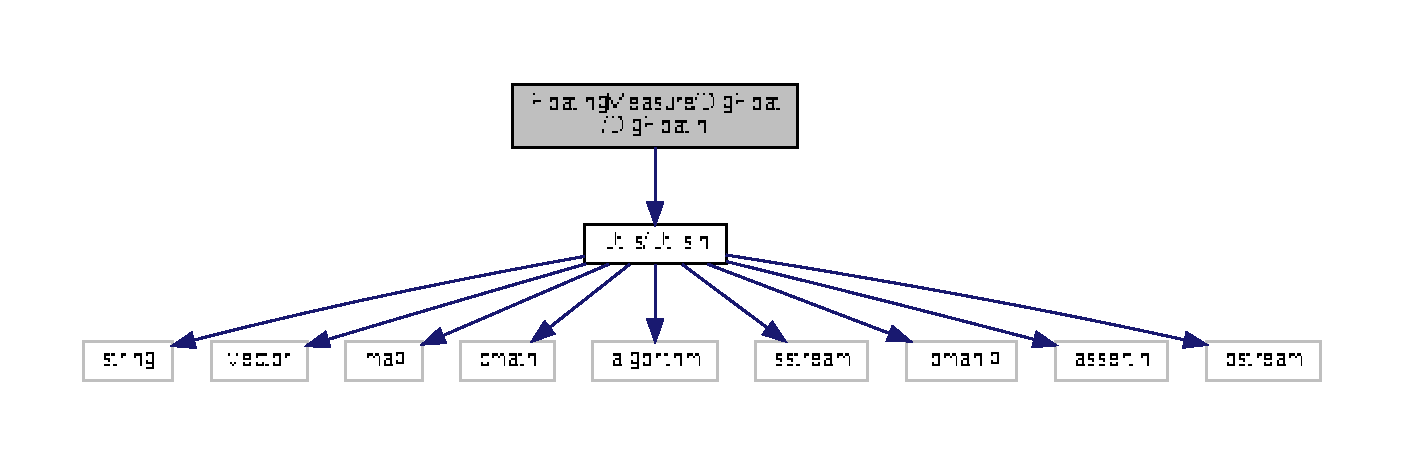
\includegraphics[width=350pt]{d1/d05/DigFloat_8h__incl}
\end{center}
\end{figure}
This graph shows which files directly or indirectly include this file\+:\nopagebreak
\begin{figure}[H]
\begin{center}
\leavevmode
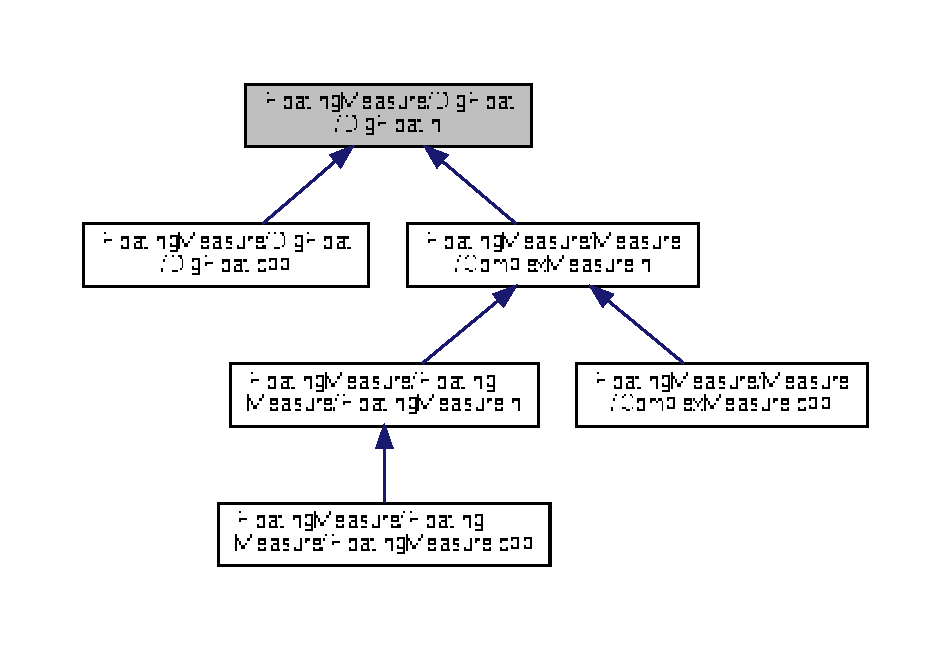
\includegraphics[width=350pt]{d1/da1/DigFloat_8h__dep__incl}
\end{center}
\end{figure}
\subsection*{Classes}
\begin{DoxyCompactItemize}
\item 
class \hyperlink{classCDigFloat}{C\+Dig\+Float}
\begin{DoxyCompactList}\small\item\em \hyperlink{classCDigFloat}{C\+Dig\+Float}\+: a class for floating point numbers which handels numerical errors of the 64 bit floating point representation.~\newline
 This class offers\+: \end{DoxyCompactList}\end{DoxyCompactItemize}
\subsection*{Macros}
\begin{DoxyCompactItemize}
\item 
\#define \hyperlink{DigFloat_8h_a7f4629d828dfb44cad8ded075fbdc392}{D\+F\+\_\+\+R\+A\+W\+\_\+\+P\+R\+I\+N\+T\+\_\+\+P\+R\+E\+C\+I\+S\+I\+ON}~40
\item 
\#define \hyperlink{DigFloat_8h_ab7dc9daaf6f33a304fe236b7cfaac808}{D\+F\+\_\+\+D\+E\+F\+A\+U\+L\+T\+\_\+\+P\+R\+I\+N\+T\+\_\+\+P\+R\+E\+C\+I\+S\+I\+ON}~10
\end{DoxyCompactItemize}
\subsection*{Functions}
\begin{DoxyCompactItemize}
\item 
\hyperlink{classCDigFloat}{C\+Dig\+Float} \hyperlink{DigFloat_8h_a269b310d675c311c6e0894bf326593ae}{abs} (const \hyperlink{classCDigFloat}{C\+Dig\+Float} \&DF)
\begin{DoxyCompactList}\small\item\em abs\+: returns \hyperlink{classCDigFloat}{C\+Dig\+Float} with absolute value; \end{DoxyCompactList}\item 
\hyperlink{classCDigFloat}{C\+Dig\+Float} \hyperlink{DigFloat_8h_a4f5706e9fe28086b245b09459f92403e}{log} (const \hyperlink{classCDigFloat}{C\+Dig\+Float} \&DF, const \hyperlink{classCDigFloat}{C\+Dig\+Float} \&df\+Base=0)
\begin{DoxyCompactList}\small\item\em log\+: returns \hyperlink{classCDigFloat}{C\+Dig\+Float} logarithm to user given base (default\+: natural logarithm with base euler number); \end{DoxyCompactList}\end{DoxyCompactItemize}


\subsection{Macro Definition Documentation}
\mbox{\Hypertarget{DigFloat_8h_ab7dc9daaf6f33a304fe236b7cfaac808}\label{DigFloat_8h_ab7dc9daaf6f33a304fe236b7cfaac808}} 
\index{Dig\+Float.\+h@{Dig\+Float.\+h}!D\+F\+\_\+\+D\+E\+F\+A\+U\+L\+T\+\_\+\+P\+R\+I\+N\+T\+\_\+\+P\+R\+E\+C\+I\+S\+I\+ON@{D\+F\+\_\+\+D\+E\+F\+A\+U\+L\+T\+\_\+\+P\+R\+I\+N\+T\+\_\+\+P\+R\+E\+C\+I\+S\+I\+ON}}
\index{D\+F\+\_\+\+D\+E\+F\+A\+U\+L\+T\+\_\+\+P\+R\+I\+N\+T\+\_\+\+P\+R\+E\+C\+I\+S\+I\+ON@{D\+F\+\_\+\+D\+E\+F\+A\+U\+L\+T\+\_\+\+P\+R\+I\+N\+T\+\_\+\+P\+R\+E\+C\+I\+S\+I\+ON}!Dig\+Float.\+h@{Dig\+Float.\+h}}
\subsubsection{\texorpdfstring{D\+F\+\_\+\+D\+E\+F\+A\+U\+L\+T\+\_\+\+P\+R\+I\+N\+T\+\_\+\+P\+R\+E\+C\+I\+S\+I\+ON}{DF\_DEFAULT\_PRINT\_PRECISION}}
{\footnotesize\ttfamily \#define D\+F\+\_\+\+D\+E\+F\+A\+U\+L\+T\+\_\+\+P\+R\+I\+N\+T\+\_\+\+P\+R\+E\+C\+I\+S\+I\+ON~10}



Definition at line 38 of file Dig\+Float.\+h.

\mbox{\Hypertarget{DigFloat_8h_a7f4629d828dfb44cad8ded075fbdc392}\label{DigFloat_8h_a7f4629d828dfb44cad8ded075fbdc392}} 
\index{Dig\+Float.\+h@{Dig\+Float.\+h}!D\+F\+\_\+\+R\+A\+W\+\_\+\+P\+R\+I\+N\+T\+\_\+\+P\+R\+E\+C\+I\+S\+I\+ON@{D\+F\+\_\+\+R\+A\+W\+\_\+\+P\+R\+I\+N\+T\+\_\+\+P\+R\+E\+C\+I\+S\+I\+ON}}
\index{D\+F\+\_\+\+R\+A\+W\+\_\+\+P\+R\+I\+N\+T\+\_\+\+P\+R\+E\+C\+I\+S\+I\+ON@{D\+F\+\_\+\+R\+A\+W\+\_\+\+P\+R\+I\+N\+T\+\_\+\+P\+R\+E\+C\+I\+S\+I\+ON}!Dig\+Float.\+h@{Dig\+Float.\+h}}
\subsubsection{\texorpdfstring{D\+F\+\_\+\+R\+A\+W\+\_\+\+P\+R\+I\+N\+T\+\_\+\+P\+R\+E\+C\+I\+S\+I\+ON}{DF\_RAW\_PRINT\_PRECISION}}
{\footnotesize\ttfamily \#define D\+F\+\_\+\+R\+A\+W\+\_\+\+P\+R\+I\+N\+T\+\_\+\+P\+R\+E\+C\+I\+S\+I\+ON~40}



Definition at line 37 of file Dig\+Float.\+h.



\subsection{Function Documentation}
\mbox{\Hypertarget{DigFloat_8h_a269b310d675c311c6e0894bf326593ae}\label{DigFloat_8h_a269b310d675c311c6e0894bf326593ae}} 
\index{Dig\+Float.\+h@{Dig\+Float.\+h}!abs@{abs}}
\index{abs@{abs}!Dig\+Float.\+h@{Dig\+Float.\+h}}
\subsubsection{\texorpdfstring{abs()}{abs()}}
{\footnotesize\ttfamily \hyperlink{classCDigFloat}{C\+Dig\+Float} abs (\begin{DoxyParamCaption}\item[{const \hyperlink{classCDigFloat}{C\+Dig\+Float} \&}]{DF }\end{DoxyParamCaption})}



abs\+: returns \hyperlink{classCDigFloat}{C\+Dig\+Float} with absolute value; 


\begin{DoxyParams}{Parameters}
{\em FM} & \hyperlink{classCDigFloat}{C\+Dig\+Float} \\
\hline
\end{DoxyParams}
\begin{DoxyReturn}{Returns}
\hyperlink{classCDigFloat}{C\+Dig\+Float} 
\end{DoxyReturn}


Definition at line 305 of file Dig\+Float.\+cpp.



References C\+Dig\+Float\+::\+Raw\+Value().

\mbox{\Hypertarget{DigFloat_8h_a4f5706e9fe28086b245b09459f92403e}\label{DigFloat_8h_a4f5706e9fe28086b245b09459f92403e}} 
\index{Dig\+Float.\+h@{Dig\+Float.\+h}!log@{log}}
\index{log@{log}!Dig\+Float.\+h@{Dig\+Float.\+h}}
\subsubsection{\texorpdfstring{log()}{log()}}
{\footnotesize\ttfamily \hyperlink{classCDigFloat}{C\+Dig\+Float} log (\begin{DoxyParamCaption}\item[{const \hyperlink{classCDigFloat}{C\+Dig\+Float} \&}]{DF,  }\item[{const \hyperlink{classCDigFloat}{C\+Dig\+Float} \&}]{df\+Base = {\ttfamily 0} }\end{DoxyParamCaption})}



log\+: returns \hyperlink{classCDigFloat}{C\+Dig\+Float} logarithm to user given base (default\+: natural logarithm with base euler number); 


\begin{DoxyParams}{Parameters}
{\em DF} & \hyperlink{classCDigFloat}{C\+Dig\+Float} \\
\hline
{\em df\+Base} & \hyperlink{classCDigFloat}{C\+Dig\+Float} as base (optional) \\
\hline
\end{DoxyParams}
\begin{DoxyReturn}{Returns}
\hyperlink{classCDigFloat}{C\+Dig\+Float} 
\end{DoxyReturn}


Definition at line 312 of file Dig\+Float.\+cpp.



References C\+Dig\+Float\+::d\+Error, C\+Dig\+Float\+::\+Error(), my\+N\+AN, C\+Dig\+Float\+::\+Raw\+Value(), C\+Dig\+Float\+::\+Value\+Max\+Limit(), and C\+Dig\+Float\+::\+Value\+Min\+Limit().


\hypertarget{FloatingMeasure_8cpp}{}\section{Floating\+Measure/\+Floating\+Measure/\+Floating\+Measure.cpp File Reference}
\label{FloatingMeasure_8cpp}\index{Floating\+Measure/\+Floating\+Measure/\+Floating\+Measure.\+cpp@{Floating\+Measure/\+Floating\+Measure/\+Floating\+Measure.\+cpp}}
{\ttfamily \#include \char`\"{}Floating\+Measure.\+h\char`\"{}}\newline
Include dependency graph for Floating\+Measure.\+cpp\+:\nopagebreak
\begin{figure}[H]
\begin{center}
\leavevmode
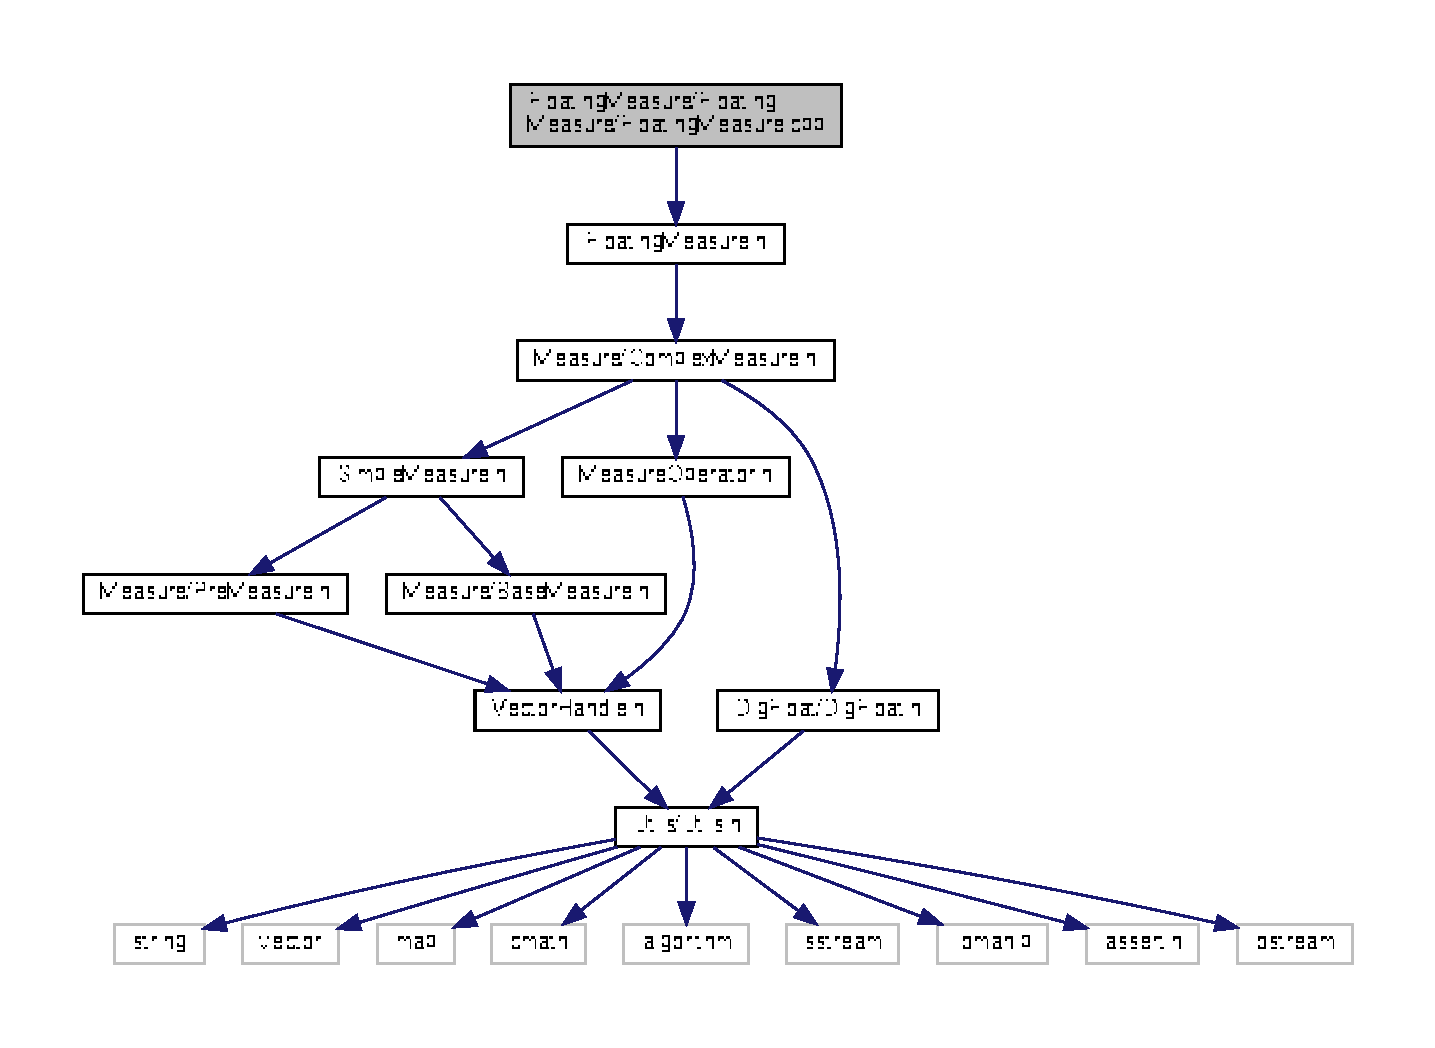
\includegraphics[width=350pt]{da/d50/FloatingMeasure_8cpp__incl}
\end{center}
\end{figure}
\subsection*{Functions}
\begin{DoxyCompactItemize}
\item 
\hyperlink{classCFloatingMeasure}{C\+Floating\+Measure} \hyperlink{FloatingMeasure_8cpp_aed62b825ab573a6d5d50c27a7f2e4d77}{abs} (const \hyperlink{classCFloatingMeasure}{C\+Floating\+Measure} \&FM)
\begin{DoxyCompactList}\small\item\em abs\+: returns \hyperlink{classCFloatingMeasure}{C\+Floating\+Measure} with absolute value; \end{DoxyCompactList}\end{DoxyCompactItemize}


\subsection{Function Documentation}
\mbox{\Hypertarget{FloatingMeasure_8cpp_aed62b825ab573a6d5d50c27a7f2e4d77}\label{FloatingMeasure_8cpp_aed62b825ab573a6d5d50c27a7f2e4d77}} 
\index{Floating\+Measure.\+cpp@{Floating\+Measure.\+cpp}!abs@{abs}}
\index{abs@{abs}!Floating\+Measure.\+cpp@{Floating\+Measure.\+cpp}}
\subsubsection{\texorpdfstring{abs()}{abs()}}
{\footnotesize\ttfamily \hyperlink{classCFloatingMeasure}{C\+Floating\+Measure} abs (\begin{DoxyParamCaption}\item[{const \hyperlink{classCFloatingMeasure}{C\+Floating\+Measure} \&}]{FM }\end{DoxyParamCaption})}



abs\+: returns \hyperlink{classCFloatingMeasure}{C\+Floating\+Measure} with absolute value; 


\begin{DoxyParams}{Parameters}
{\em FM} & \hyperlink{classCFloatingMeasure}{C\+Floating\+Measure} \\
\hline
\end{DoxyParams}
\begin{DoxyReturn}{Returns}
\hyperlink{classCFloatingMeasure}{C\+Floating\+Measure} 
\end{DoxyReturn}


Definition at line 413 of file Floating\+Measure.\+cpp.



References abs(), C\+Floating\+Measure\+::\+C\+Floating\+Measure(), C\+Floating\+Measure\+::\+Floating(), and C\+Floating\+Measure\+::\+Measure().


\hypertarget{FloatingMeasure_8h}{}\section{Floating\+Measure/\+Floating\+Measure/\+Floating\+Measure.h File Reference}
\label{FloatingMeasure_8h}\index{Floating\+Measure/\+Floating\+Measure/\+Floating\+Measure.\+h@{Floating\+Measure/\+Floating\+Measure/\+Floating\+Measure.\+h}}
{\ttfamily \#include $<$Measure/\+Complex\+Measure.\+h$>$}\newline
Include dependency graph for Floating\+Measure.\+h\+:
\nopagebreak
\begin{figure}[H]
\begin{center}
\leavevmode
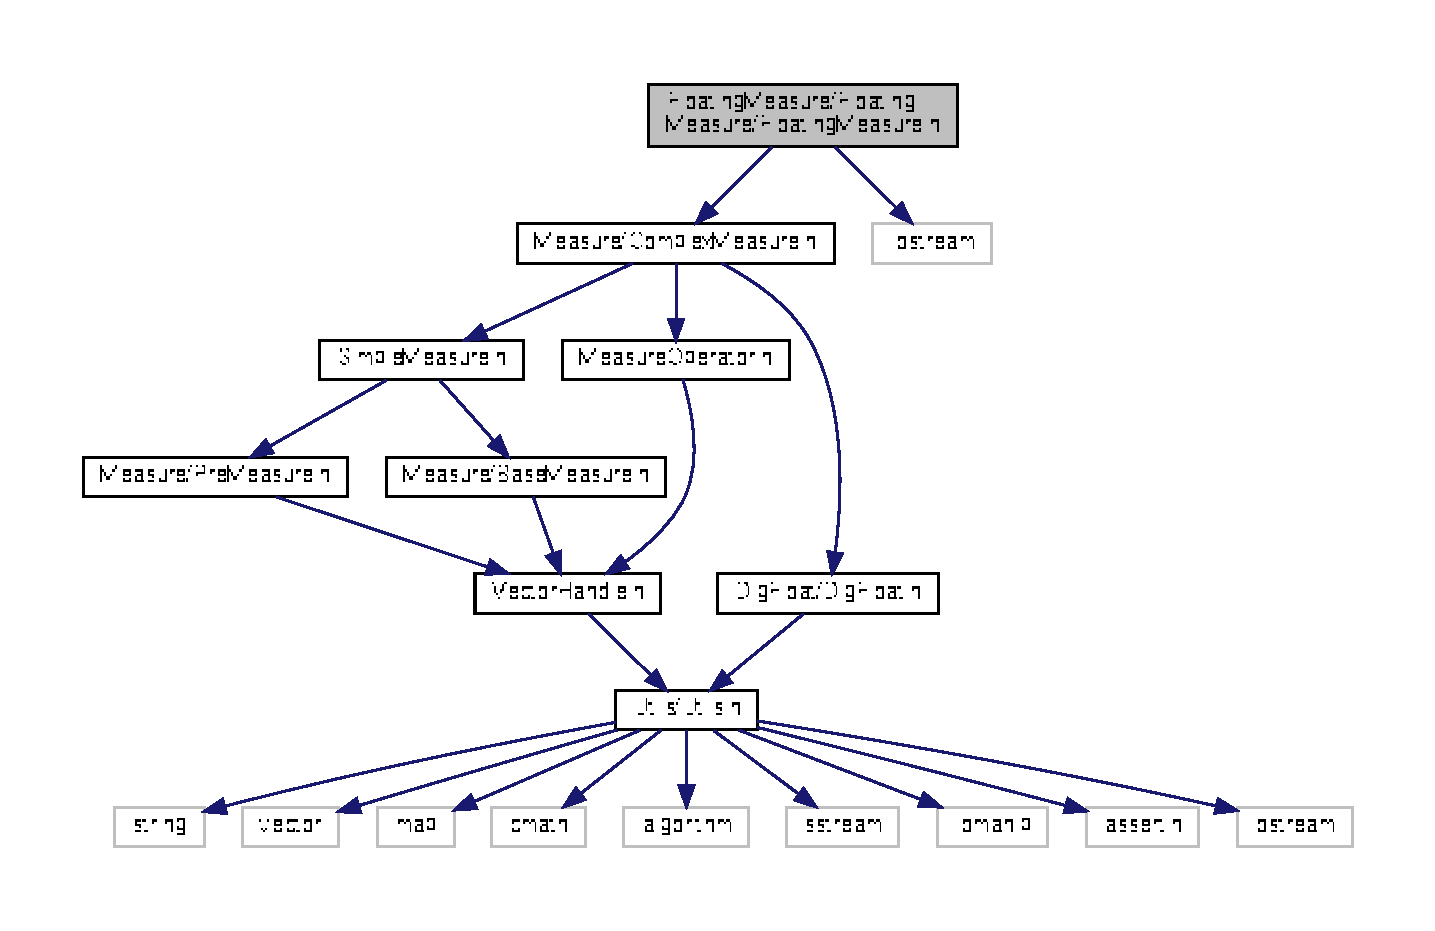
\includegraphics[width=350pt]{da/dd8/FloatingMeasure_8h__incl}
\end{center}
\end{figure}
This graph shows which files directly or indirectly include this file\+:
\nopagebreak
\begin{figure}[H]
\begin{center}
\leavevmode
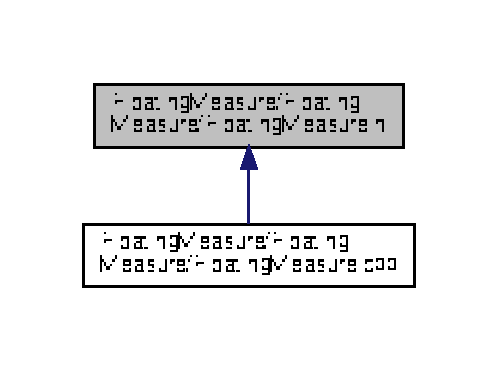
\includegraphics[width=239pt]{dd/dbe/FloatingMeasure_8h__dep__incl}
\end{center}
\end{figure}
\subsection*{Classes}
\begin{DoxyCompactItemize}
\item 
class \hyperlink{classCFloatingMeasure}{C\+Floating\+Measure}
\begin{DoxyCompactList}\small\item\em Floating\+Measure\+: represents a floating number with a complex measure (e.\+g. 10$\ast$m/s). This class offers\+: \end{DoxyCompactList}\end{DoxyCompactItemize}
\subsection*{Functions}
\begin{DoxyCompactItemize}
\item 
\hyperlink{classCFloatingMeasure}{C\+Floating\+Measure} \hyperlink{FloatingMeasure_8h_aed62b825ab573a6d5d50c27a7f2e4d77}{abs} (const \hyperlink{classCFloatingMeasure}{C\+Floating\+Measure} \&FM)
\begin{DoxyCompactList}\small\item\em abs\+: returns \hyperlink{classCFloatingMeasure}{C\+Floating\+Measure} with absolute value; \end{DoxyCompactList}\item 
\hyperlink{classCFloatingMeasure}{C\+Floating\+Measure} \hyperlink{FloatingMeasure_8h_a510e0349b3e04c276027c4555d4befd7}{operator$\ast$} (const \hyperlink{classCDigFloat}{C\+Dig\+Float} \&Floating, const \hyperlink{classCComplexMeasure}{C\+Complex\+Measure} \&Measure)
\begin{DoxyCompactList}\small\item\em operator$\ast$ \+: enables \hyperlink{classCFloatingMeasure}{C\+Floating\+Measure} = 10$\ast$mV; \end{DoxyCompactList}\item 
\hyperlink{classCFloatingMeasure}{C\+Floating\+Measure} \hyperlink{FloatingMeasure_8h_a9237848af0e386f79e22b1fb4167b49e}{operator$\ast$} (const \hyperlink{classCComplexMeasure}{C\+Complex\+Measure} \&Measure, const \hyperlink{classCDigFloat}{C\+Dig\+Float} \&Floating)
\begin{DoxyCompactList}\small\item\em operator$\ast$ \+: enables \hyperlink{classCFloatingMeasure}{C\+Floating\+Measure} = m\+V$\ast$10; \end{DoxyCompactList}\item 
\hyperlink{classCFloatingMeasure}{C\+Floating\+Measure} \hyperlink{FloatingMeasure_8h_a4411f7957eb8eb682cfd15be04918cae}{operator$\ast$} (const \hyperlink{classCFloatingMeasure}{C\+Floating\+Measure} \&Floating\+Measure, const \hyperlink{classCComplexMeasure}{C\+Complex\+Measure} \&Measure)
\begin{DoxyCompactList}\small\item\em operator$\ast$ \+: enables \hyperlink{classCFloatingMeasure}{C\+Floating\+Measure} = 10$\ast$m\+V$\ast$uA; \end{DoxyCompactList}\item 
\hyperlink{classCFloatingMeasure}{C\+Floating\+Measure} \hyperlink{FloatingMeasure_8h_a7ffe3aec493a30227a84a15665ad5c9b}{operator$\ast$} (const \hyperlink{classCComplexMeasure}{C\+Complex\+Measure} \&Measure, const \hyperlink{classCFloatingMeasure}{C\+Floating\+Measure} \&Floating\+Measure)
\begin{DoxyCompactList}\small\item\em operator$\ast$ \+: enables \hyperlink{classCFloatingMeasure}{C\+Floating\+Measure} = m\+V$\ast$u\+A$\ast$10; \end{DoxyCompactList}\item 
\hyperlink{classCFloatingMeasure}{C\+Floating\+Measure} \hyperlink{FloatingMeasure_8h_a38b04a23f627da9a70f22a69d4ac35ac}{operator/} (const \hyperlink{classCDigFloat}{C\+Dig\+Float} \&Floating, const \hyperlink{classCComplexMeasure}{C\+Complex\+Measure} \&Measure)
\begin{DoxyCompactList}\small\item\em operator/ \+: enables \hyperlink{classCFloatingMeasure}{C\+Floating\+Measure} = 10/mV; \end{DoxyCompactList}\item 
\hyperlink{classCFloatingMeasure}{C\+Floating\+Measure} \hyperlink{FloatingMeasure_8h_ad1ee707b3ca8af2b462c8e6ccafd7f46}{operator/} (const \hyperlink{classCComplexMeasure}{C\+Complex\+Measure} \&Measure, const \hyperlink{classCDigFloat}{C\+Dig\+Float} \&Floating)
\begin{DoxyCompactList}\small\item\em operator/ \+: enables \hyperlink{classCFloatingMeasure}{C\+Floating\+Measure} = m\+V/10; \end{DoxyCompactList}\item 
\hyperlink{classCFloatingMeasure}{C\+Floating\+Measure} \hyperlink{FloatingMeasure_8h_a69c15c6d9c995a192ccdb14c29ef0439}{operator/} (const \hyperlink{classCFloatingMeasure}{C\+Floating\+Measure} \&Floating\+Measure, const \hyperlink{classCComplexMeasure}{C\+Complex\+Measure} \&Measure)
\begin{DoxyCompactList}\small\item\em operator/ \+: enables \hyperlink{classCFloatingMeasure}{C\+Floating\+Measure} = 10$\ast$m\+V/uA; \end{DoxyCompactList}\end{DoxyCompactItemize}


\subsection{Function Documentation}
\mbox{\Hypertarget{FloatingMeasure_8h_aed62b825ab573a6d5d50c27a7f2e4d77}\label{FloatingMeasure_8h_aed62b825ab573a6d5d50c27a7f2e4d77}} 
\index{Floating\+Measure.\+h@{Floating\+Measure.\+h}!abs@{abs}}
\index{abs@{abs}!Floating\+Measure.\+h@{Floating\+Measure.\+h}}
\subsubsection{\texorpdfstring{abs()}{abs()}}
{\footnotesize\ttfamily \hyperlink{classCFloatingMeasure}{C\+Floating\+Measure} abs (\begin{DoxyParamCaption}\item[{const \hyperlink{classCFloatingMeasure}{C\+Floating\+Measure} \&}]{FM }\end{DoxyParamCaption})}



abs\+: returns \hyperlink{classCFloatingMeasure}{C\+Floating\+Measure} with absolute value; 


\begin{DoxyParams}{Parameters}
{\em FM} & \hyperlink{classCFloatingMeasure}{C\+Floating\+Measure} \\
\hline
\end{DoxyParams}
\begin{DoxyReturn}{Returns}
\hyperlink{classCFloatingMeasure}{C\+Floating\+Measure} 
\end{DoxyReturn}


Definition at line 332 of file Floating\+Measure.\+cpp.



References abs(), C\+Floating\+Measure\+::\+C\+Floating\+Measure(), C\+Floating\+Measure\+::\+Floating(), and C\+Floating\+Measure\+::\+Measure().

\mbox{\Hypertarget{FloatingMeasure_8h_a510e0349b3e04c276027c4555d4befd7}\label{FloatingMeasure_8h_a510e0349b3e04c276027c4555d4befd7}} 
\index{Floating\+Measure.\+h@{Floating\+Measure.\+h}!operator$\ast$@{operator$\ast$}}
\index{operator$\ast$@{operator$\ast$}!Floating\+Measure.\+h@{Floating\+Measure.\+h}}
\subsubsection{\texorpdfstring{operator$\ast$()}{operator*()}\hspace{0.1cm}{\footnotesize\ttfamily [1/4]}}
{\footnotesize\ttfamily \hyperlink{classCFloatingMeasure}{C\+Floating\+Measure} operator$\ast$ (\begin{DoxyParamCaption}\item[{const \hyperlink{classCDigFloat}{C\+Dig\+Float} \&}]{Floating,  }\item[{const \hyperlink{classCComplexMeasure}{C\+Complex\+Measure} \&}]{Measure }\end{DoxyParamCaption})}



operator$\ast$ \+: enables \hyperlink{classCFloatingMeasure}{C\+Floating\+Measure} = 10$\ast$mV; 


\begin{DoxyParams}{Parameters}
{\em Floating} & \hyperlink{classCDigFloat}{C\+Dig\+Float} \\
\hline
{\em Measure} & \hyperlink{classCComplexMeasure}{C\+Complex\+Measure} \\
\hline
\end{DoxyParams}
\begin{DoxyReturn}{Returns}
\hyperlink{classCFloatingMeasure}{C\+Floating\+Measure} 
\end{DoxyReturn}


Definition at line 390 of file Floating\+Measure.\+h.



References C\+Complex\+Measure\+::\+C\+Floating\+Measure.

\mbox{\Hypertarget{FloatingMeasure_8h_a9237848af0e386f79e22b1fb4167b49e}\label{FloatingMeasure_8h_a9237848af0e386f79e22b1fb4167b49e}} 
\index{Floating\+Measure.\+h@{Floating\+Measure.\+h}!operator$\ast$@{operator$\ast$}}
\index{operator$\ast$@{operator$\ast$}!Floating\+Measure.\+h@{Floating\+Measure.\+h}}
\subsubsection{\texorpdfstring{operator$\ast$()}{operator*()}\hspace{0.1cm}{\footnotesize\ttfamily [2/4]}}
{\footnotesize\ttfamily \hyperlink{classCFloatingMeasure}{C\+Floating\+Measure} operator$\ast$ (\begin{DoxyParamCaption}\item[{const \hyperlink{classCComplexMeasure}{C\+Complex\+Measure} \&}]{Measure,  }\item[{const \hyperlink{classCDigFloat}{C\+Dig\+Float} \&}]{Floating }\end{DoxyParamCaption})}



operator$\ast$ \+: enables \hyperlink{classCFloatingMeasure}{C\+Floating\+Measure} = m\+V$\ast$10; 


\begin{DoxyParams}{Parameters}
{\em Measure} & \hyperlink{classCComplexMeasure}{C\+Complex\+Measure} \\
\hline
{\em Floating} & \hyperlink{classCDigFloat}{C\+Dig\+Float} \\
\hline
\end{DoxyParams}
\begin{DoxyReturn}{Returns}
\hyperlink{classCFloatingMeasure}{C\+Floating\+Measure} 
\end{DoxyReturn}


Definition at line 399 of file Floating\+Measure.\+h.



References C\+Complex\+Measure\+::\+C\+Floating\+Measure.

\mbox{\Hypertarget{FloatingMeasure_8h_a4411f7957eb8eb682cfd15be04918cae}\label{FloatingMeasure_8h_a4411f7957eb8eb682cfd15be04918cae}} 
\index{Floating\+Measure.\+h@{Floating\+Measure.\+h}!operator$\ast$@{operator$\ast$}}
\index{operator$\ast$@{operator$\ast$}!Floating\+Measure.\+h@{Floating\+Measure.\+h}}
\subsubsection{\texorpdfstring{operator$\ast$()}{operator*()}\hspace{0.1cm}{\footnotesize\ttfamily [3/4]}}
{\footnotesize\ttfamily \hyperlink{classCFloatingMeasure}{C\+Floating\+Measure} operator$\ast$ (\begin{DoxyParamCaption}\item[{const \hyperlink{classCFloatingMeasure}{C\+Floating\+Measure} \&}]{Floating\+Measure,  }\item[{const \hyperlink{classCComplexMeasure}{C\+Complex\+Measure} \&}]{Measure }\end{DoxyParamCaption})}



operator$\ast$ \+: enables \hyperlink{classCFloatingMeasure}{C\+Floating\+Measure} = 10$\ast$m\+V$\ast$uA; 


\begin{DoxyParams}{Parameters}
{\em Floating\+Measure} & \hyperlink{classCFloatingMeasure}{C\+Floating\+Measure} (e.\+g. 10$\ast$mV) \\
\hline
{\em Measure} & \hyperlink{classCComplexMeasure}{C\+Complex\+Measure} (e.\+g. uA) \\
\hline
\end{DoxyParams}
\begin{DoxyReturn}{Returns}
\hyperlink{classCFloatingMeasure}{C\+Floating\+Measure} 
\end{DoxyReturn}


Definition at line 408 of file Floating\+Measure.\+h.



References C\+Complex\+Measure\+::\+C\+Floating\+Measure, C\+Floating\+Measure\+::\+Floating(), and C\+Floating\+Measure\+::\+Measure().

\mbox{\Hypertarget{FloatingMeasure_8h_a7ffe3aec493a30227a84a15665ad5c9b}\label{FloatingMeasure_8h_a7ffe3aec493a30227a84a15665ad5c9b}} 
\index{Floating\+Measure.\+h@{Floating\+Measure.\+h}!operator$\ast$@{operator$\ast$}}
\index{operator$\ast$@{operator$\ast$}!Floating\+Measure.\+h@{Floating\+Measure.\+h}}
\subsubsection{\texorpdfstring{operator$\ast$()}{operator*()}\hspace{0.1cm}{\footnotesize\ttfamily [4/4]}}
{\footnotesize\ttfamily \hyperlink{classCFloatingMeasure}{C\+Floating\+Measure} operator$\ast$ (\begin{DoxyParamCaption}\item[{const \hyperlink{classCComplexMeasure}{C\+Complex\+Measure} \&}]{Measure,  }\item[{const \hyperlink{classCFloatingMeasure}{C\+Floating\+Measure} \&}]{Floating\+Measure }\end{DoxyParamCaption})}



operator$\ast$ \+: enables \hyperlink{classCFloatingMeasure}{C\+Floating\+Measure} = m\+V$\ast$u\+A$\ast$10; 


\begin{DoxyParams}{Parameters}
{\em Measure} & \hyperlink{classCComplexMeasure}{C\+Complex\+Measure} (e.\+g. m\+V$\ast$uA) \\
\hline
{\em Floating\+Measure} & \hyperlink{classCFloatingMeasure}{C\+Floating\+Measure} (e.\+g. 10) \\
\hline
\end{DoxyParams}
\begin{DoxyReturn}{Returns}
\hyperlink{classCFloatingMeasure}{C\+Floating\+Measure} 
\end{DoxyReturn}


Definition at line 417 of file Floating\+Measure.\+h.



References C\+Complex\+Measure\+::\+C\+Floating\+Measure, C\+Floating\+Measure\+::\+Floating(), and C\+Floating\+Measure\+::\+Measure().

\mbox{\Hypertarget{FloatingMeasure_8h_a38b04a23f627da9a70f22a69d4ac35ac}\label{FloatingMeasure_8h_a38b04a23f627da9a70f22a69d4ac35ac}} 
\index{Floating\+Measure.\+h@{Floating\+Measure.\+h}!operator/@{operator/}}
\index{operator/@{operator/}!Floating\+Measure.\+h@{Floating\+Measure.\+h}}
\subsubsection{\texorpdfstring{operator/()}{operator/()}\hspace{0.1cm}{\footnotesize\ttfamily [1/3]}}
{\footnotesize\ttfamily \hyperlink{classCFloatingMeasure}{C\+Floating\+Measure} operator/ (\begin{DoxyParamCaption}\item[{const \hyperlink{classCDigFloat}{C\+Dig\+Float} \&}]{Floating,  }\item[{const \hyperlink{classCComplexMeasure}{C\+Complex\+Measure} \&}]{Measure }\end{DoxyParamCaption})}



operator/ \+: enables \hyperlink{classCFloatingMeasure}{C\+Floating\+Measure} = 10/mV; 


\begin{DoxyParams}{Parameters}
{\em Floating} & \hyperlink{classCDigFloat}{C\+Dig\+Float} \\
\hline
{\em Measure} & \hyperlink{classCComplexMeasure}{C\+Complex\+Measure} \\
\hline
\end{DoxyParams}
\begin{DoxyReturn}{Returns}
\hyperlink{classCFloatingMeasure}{C\+Floating\+Measure} 
\end{DoxyReturn}


Definition at line 426 of file Floating\+Measure.\+h.



References bm\+Number, C\+Complex\+Measure\+::\+C\+Complex\+Measure(), C\+Complex\+Measure\+::\+C\+Floating\+Measure, and pm\+Ident.

\mbox{\Hypertarget{FloatingMeasure_8h_ad1ee707b3ca8af2b462c8e6ccafd7f46}\label{FloatingMeasure_8h_ad1ee707b3ca8af2b462c8e6ccafd7f46}} 
\index{Floating\+Measure.\+h@{Floating\+Measure.\+h}!operator/@{operator/}}
\index{operator/@{operator/}!Floating\+Measure.\+h@{Floating\+Measure.\+h}}
\subsubsection{\texorpdfstring{operator/()}{operator/()}\hspace{0.1cm}{\footnotesize\ttfamily [2/3]}}
{\footnotesize\ttfamily \hyperlink{classCFloatingMeasure}{C\+Floating\+Measure} operator/ (\begin{DoxyParamCaption}\item[{const \hyperlink{classCComplexMeasure}{C\+Complex\+Measure} \&}]{Measure,  }\item[{const \hyperlink{classCDigFloat}{C\+Dig\+Float} \&}]{Floating }\end{DoxyParamCaption})}



operator/ \+: enables \hyperlink{classCFloatingMeasure}{C\+Floating\+Measure} = m\+V/10; 


\begin{DoxyParams}{Parameters}
{\em Measure} & \hyperlink{classCComplexMeasure}{C\+Complex\+Measure} \\
\hline
{\em Floating} & \hyperlink{classCDigFloat}{C\+Dig\+Float} \\
\hline
\end{DoxyParams}
\begin{DoxyReturn}{Returns}
\hyperlink{classCFloatingMeasure}{C\+Floating\+Measure} 
\end{DoxyReturn}


Definition at line 435 of file Floating\+Measure.\+h.



References bm\+Number, C\+Complex\+Measure\+::\+C\+Complex\+Measure(), C\+Complex\+Measure\+::\+C\+Floating\+Measure, and pm\+Ident.

\mbox{\Hypertarget{FloatingMeasure_8h_a69c15c6d9c995a192ccdb14c29ef0439}\label{FloatingMeasure_8h_a69c15c6d9c995a192ccdb14c29ef0439}} 
\index{Floating\+Measure.\+h@{Floating\+Measure.\+h}!operator/@{operator/}}
\index{operator/@{operator/}!Floating\+Measure.\+h@{Floating\+Measure.\+h}}
\subsubsection{\texorpdfstring{operator/()}{operator/()}\hspace{0.1cm}{\footnotesize\ttfamily [3/3]}}
{\footnotesize\ttfamily \hyperlink{classCFloatingMeasure}{C\+Floating\+Measure} operator/ (\begin{DoxyParamCaption}\item[{const \hyperlink{classCFloatingMeasure}{C\+Floating\+Measure} \&}]{Floating\+Measure,  }\item[{const \hyperlink{classCComplexMeasure}{C\+Complex\+Measure} \&}]{Measure }\end{DoxyParamCaption})}



operator/ \+: enables \hyperlink{classCFloatingMeasure}{C\+Floating\+Measure} = 10$\ast$m\+V/uA; 


\begin{DoxyParams}{Parameters}
{\em Floating\+Measure} & \hyperlink{classCFloatingMeasure}{C\+Floating\+Measure} (e.\+g. 10$\ast$mV) \\
\hline
{\em Measure} & \hyperlink{classCComplexMeasure}{C\+Complex\+Measure} (e.\+g. uA) \\
\hline
\end{DoxyParams}
\begin{DoxyReturn}{Returns}
\hyperlink{classCFloatingMeasure}{C\+Floating\+Measure} 
\end{DoxyReturn}


Definition at line 444 of file Floating\+Measure.\+h.



References C\+Complex\+Measure\+::\+C\+Floating\+Measure, C\+Floating\+Measure\+::\+Floating(), and C\+Floating\+Measure\+::\+Measure().


\hypertarget{BaseMeasure_8cpp}{}\section{Floating\+Measure/\+Measure/\+Base\+Measure.cpp File Reference}
\label{BaseMeasure_8cpp}\index{Floating\+Measure/\+Measure/\+Base\+Measure.\+cpp@{Floating\+Measure/\+Measure/\+Base\+Measure.\+cpp}}
{\ttfamily \#include \char`\"{}Base\+Measure.\+h\char`\"{}}\newline
Include dependency graph for Base\+Measure.\+cpp\+:
\nopagebreak
\begin{figure}[H]
\begin{center}
\leavevmode
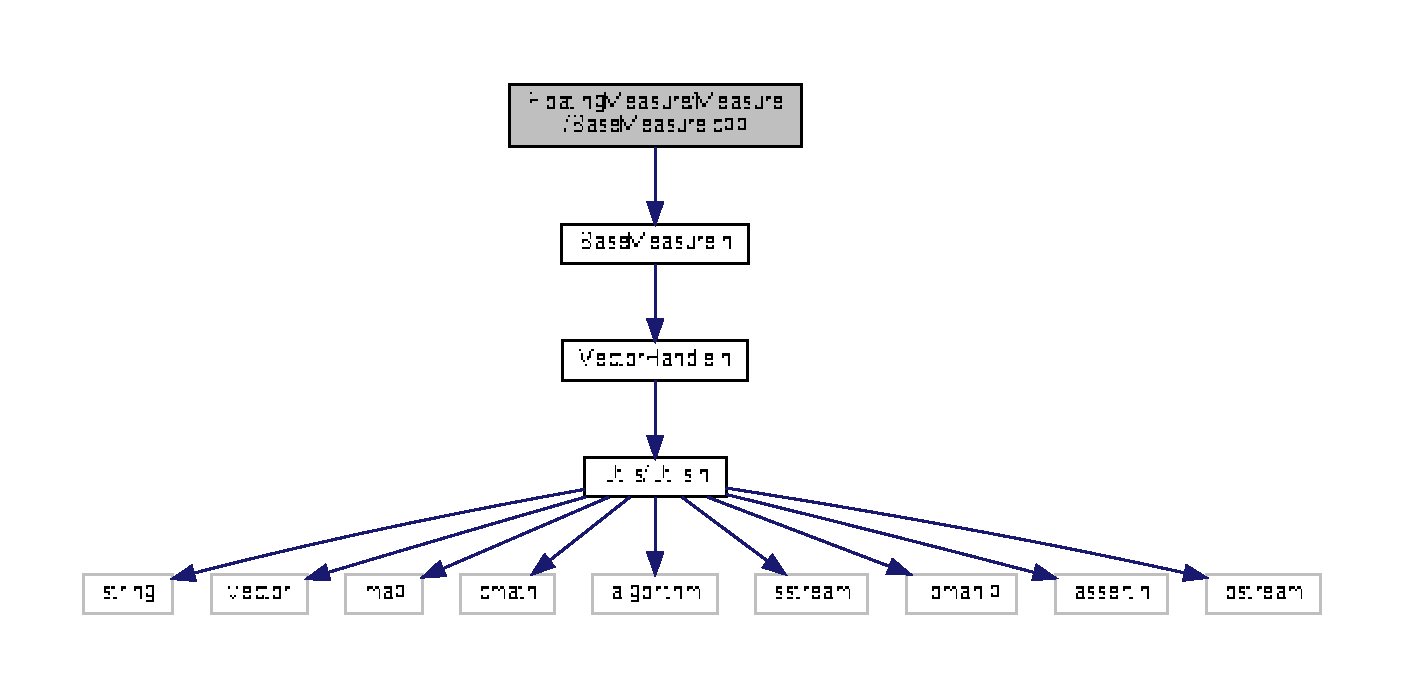
\includegraphics[width=350pt]{d3/de1/BaseMeasure_8cpp__incl}
\end{center}
\end{figure}

\hypertarget{BaseMeasure_8h}{}\section{Floating\+Measure/\+Measure/\+Base\+Measure.h File Reference}
\label{BaseMeasure_8h}\index{Floating\+Measure/\+Measure/\+Base\+Measure.\+h@{Floating\+Measure/\+Measure/\+Base\+Measure.\+h}}
{\ttfamily \#include \char`\"{}Vector\+Handle.\+h\char`\"{}}\newline
Include dependency graph for Base\+Measure.\+h\+:\nopagebreak
\begin{figure}[H]
\begin{center}
\leavevmode
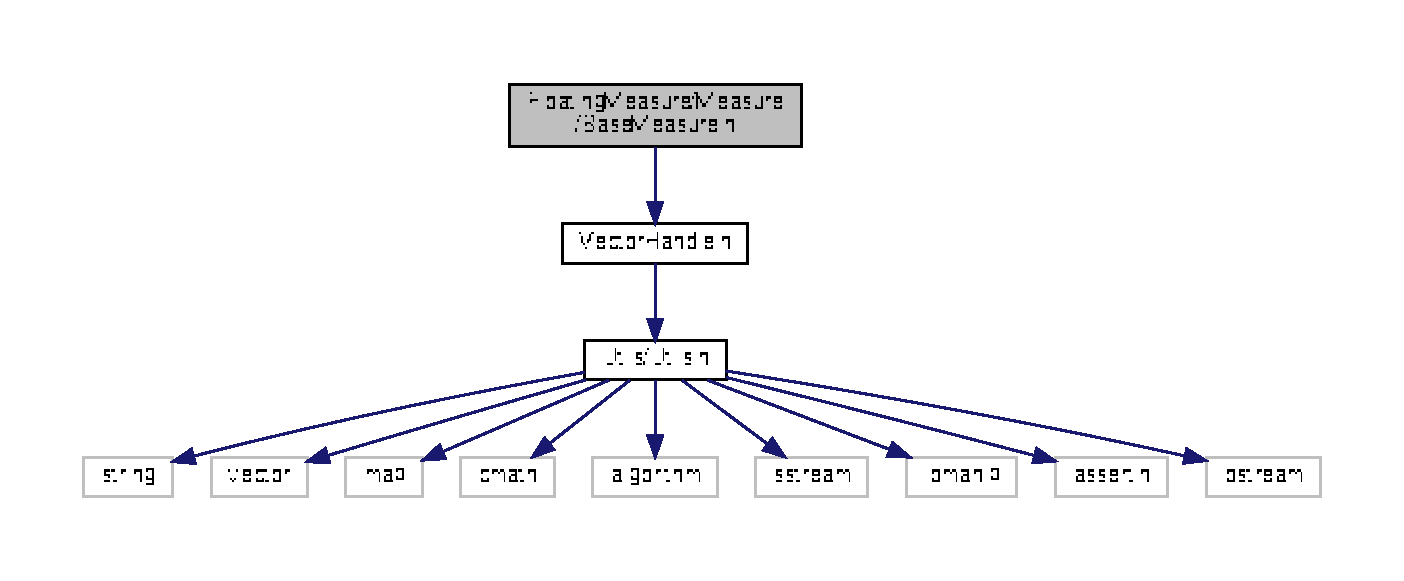
\includegraphics[width=350pt]{d8/d1f/BaseMeasure_8h__incl}
\end{center}
\end{figure}
This graph shows which files directly or indirectly include this file\+:\nopagebreak
\begin{figure}[H]
\begin{center}
\leavevmode
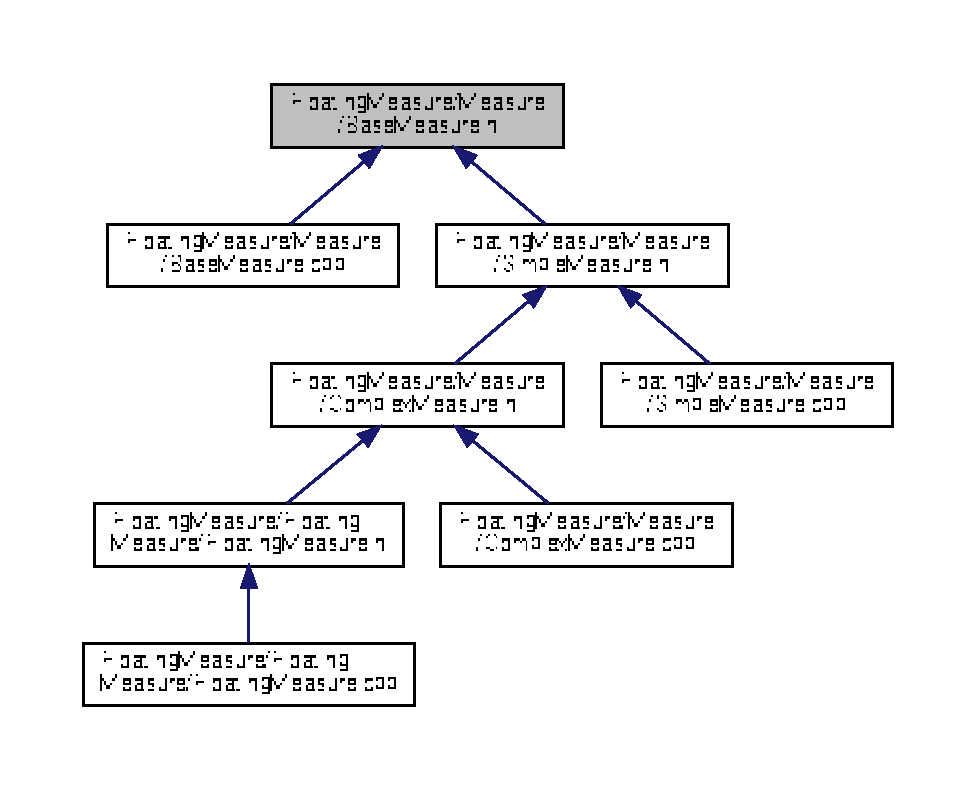
\includegraphics[width=350pt]{d5/ddc/BaseMeasure_8h__dep__incl}
\end{center}
\end{figure}
\subsection*{Classes}
\begin{DoxyCompactItemize}
\item 
class \hyperlink{classCBaseMeasure}{C\+Base\+Measure}
\begin{DoxyCompactList}\small\item\em \hyperlink{classCBaseMeasure}{C\+Base\+Measure}\+: represents the base-\/measure part of a measure.~\newline
 For example milli degree celsius consists of the base-\/measure part \char`\"{}degree celsius\char`\"{} (see \hyperlink{classCBaseMeasure}{C\+Base\+Measure}) and the pre-\/measure part \char`\"{}milli\char`\"{} (see \hyperlink{classCPreMeasure}{C\+Pre\+Measure}). ~\newline
 This class handles vectors of\+: \end{DoxyCompactList}\end{DoxyCompactItemize}
\subsection*{Macros}
\begin{DoxyCompactItemize}
\item 
\#define \hyperlink{BaseMeasure_8h_a79bcfb6bde984f42d1124b068a509af7}{B\+A\+SE}~\hyperlink{classCSingleton_a58f5ac3aaaea8079a373350594726bdf}{C\+Base\+Measure\+Singleton\+::instance}()
\begin{DoxyCompactList}\small\item\em shortcut to the singleton representation of \hyperlink{classCBaseMeasure}{C\+Base\+Measure} \end{DoxyCompactList}\end{DoxyCompactItemize}
\subsection*{Typedefs}
\begin{DoxyCompactItemize}
\item 
typedef \hyperlink{classCSingleton}{C\+Singleton}$<$ \hyperlink{classCBaseMeasure}{C\+Base\+Measure} $>$ \hyperlink{BaseMeasure_8h_a0cf675413cb12be588422a57b33cce1f}{C\+Base\+Measure\+Singleton}
\begin{DoxyCompactList}\small\item\em use \hyperlink{classCBaseMeasure}{C\+Base\+Measure} as a singleton \end{DoxyCompactList}\end{DoxyCompactItemize}
\subsection*{Enumerations}
\begin{DoxyCompactItemize}
\item 
enum \hyperlink{BaseMeasure_8h_ac90e5164ccf1f0d648fba7e94b229a11}{e\+Base\+Measure} \{ \newline
\hyperlink{BaseMeasure_8h_ac90e5164ccf1f0d648fba7e94b229a11a5c8528d80e9751805f662690f7764240}{bm\+Number} = 0, 
\hyperlink{BaseMeasure_8h_ac90e5164ccf1f0d648fba7e94b229a11a5c5770bd8b4f62e351d3f08e1c074dec}{bm\+First} = bm\+Number, 
\hyperlink{BaseMeasure_8h_ac90e5164ccf1f0d648fba7e94b229a11a662f2aa09627247b53e6f3c5cd10815e}{bm\+Volt}, 
\hyperlink{BaseMeasure_8h_ac90e5164ccf1f0d648fba7e94b229a11aa0bfa4e97216cd5d37576ed9c7124f37}{bm\+Ampere}, 
\newline
\hyperlink{BaseMeasure_8h_ac90e5164ccf1f0d648fba7e94b229a11a7d519faa41d1d34d9c378cfc61254074}{bm\+Deg\+Kelvin}, 
\hyperlink{BaseMeasure_8h_ac90e5164ccf1f0d648fba7e94b229a11a42cee40c384c9bbda9aa488151b590b4}{bm\+Deg\+Celsius}, 
\hyperlink{BaseMeasure_8h_ac90e5164ccf1f0d648fba7e94b229a11add58e3d33a5d9459dbe3bf9d3f90777c}{bm\+Deg\+Fahrenheit}, 
\hyperlink{BaseMeasure_8h_ac90e5164ccf1f0d648fba7e94b229a11a3c2b76106d8f5cd21cefc918b3487282}{bm\+Ohm}, 
\newline
\hyperlink{BaseMeasure_8h_ac90e5164ccf1f0d648fba7e94b229a11a5d8b1592b21e5fe3505a9ae4222ef85d}{bm\+Farad}, 
\hyperlink{BaseMeasure_8h_ac90e5164ccf1f0d648fba7e94b229a11af98f442616dcb74a8a3af3a05c65906a}{bm\+Hertz}, 
\hyperlink{BaseMeasure_8h_ac90e5164ccf1f0d648fba7e94b229a11a154cadadef2b87dabd57e216a5e01f08}{bm\+Second}, 
\hyperlink{BaseMeasure_8h_ac90e5164ccf1f0d648fba7e94b229a11abb3a886332014c0b0b5f872651a325a3}{bm\+Minute}, 
\newline
\hyperlink{BaseMeasure_8h_ac90e5164ccf1f0d648fba7e94b229a11afb903ec248fbb053df2e597d3962475d}{bm\+Hour}, 
\hyperlink{BaseMeasure_8h_ac90e5164ccf1f0d648fba7e94b229a11a3b3d24fe3421db3173c33e175130c71c}{bm\+Day}, 
\hyperlink{BaseMeasure_8h_ac90e5164ccf1f0d648fba7e94b229a11a648bcf7faf2a79b8e7a13e785a84295c}{bm\+Meter}, 
\hyperlink{BaseMeasure_8h_ac90e5164ccf1f0d648fba7e94b229a11aa336b6ad4081714bf4f1ba1aff14e192}{bm\+Inch}, 
\newline
\hyperlink{BaseMeasure_8h_ac90e5164ccf1f0d648fba7e94b229a11a5d3576c8ce233e10ee14736257ec240d}{bm\+Foot}, 
\hyperlink{BaseMeasure_8h_ac90e5164ccf1f0d648fba7e94b229a11a4515cdd3e54e74cbe6a74b2fbc9731fe}{bm\+Yard}, 
\hyperlink{BaseMeasure_8h_ac90e5164ccf1f0d648fba7e94b229a11af69da55a5568ae3c6b417879e4eb22c4}{bm\+Mile}, 
\hyperlink{BaseMeasure_8h_ac90e5164ccf1f0d648fba7e94b229a11a51111031ebb3a92041aa8821dc0bf076}{bm\+Last}, 
\newline
\hyperlink{BaseMeasure_8h_ac90e5164ccf1f0d648fba7e94b229a11ac30190fee6f86e2f76b96886533f74d8}{bm\+Unknown} = bm\+Last
 \}\begin{DoxyCompactList}\small\item\em enum for indexing the vectors of \hyperlink{classCBaseMeasure}{C\+Base\+Measure} \end{DoxyCompactList}
\end{DoxyCompactItemize}


\subsection{Macro Definition Documentation}
\mbox{\Hypertarget{BaseMeasure_8h_a79bcfb6bde984f42d1124b068a509af7}\label{BaseMeasure_8h_a79bcfb6bde984f42d1124b068a509af7}} 
\index{Base\+Measure.\+h@{Base\+Measure.\+h}!B\+A\+SE@{B\+A\+SE}}
\index{B\+A\+SE@{B\+A\+SE}!Base\+Measure.\+h@{Base\+Measure.\+h}}
\subsubsection{\texorpdfstring{B\+A\+SE}{BASE}}
{\footnotesize\ttfamily \#define B\+A\+SE~\hyperlink{classCSingleton_a58f5ac3aaaea8079a373350594726bdf}{C\+Base\+Measure\+Singleton\+::instance}()}



shortcut to the singleton representation of \hyperlink{classCBaseMeasure}{C\+Base\+Measure} 



Definition at line 183 of file Base\+Measure.\+h.



\subsection{Typedef Documentation}
\mbox{\Hypertarget{BaseMeasure_8h_a0cf675413cb12be588422a57b33cce1f}\label{BaseMeasure_8h_a0cf675413cb12be588422a57b33cce1f}} 
\index{Base\+Measure.\+h@{Base\+Measure.\+h}!C\+Base\+Measure\+Singleton@{C\+Base\+Measure\+Singleton}}
\index{C\+Base\+Measure\+Singleton@{C\+Base\+Measure\+Singleton}!Base\+Measure.\+h@{Base\+Measure.\+h}}
\subsubsection{\texorpdfstring{C\+Base\+Measure\+Singleton}{CBaseMeasureSingleton}}
{\footnotesize\ttfamily typedef \hyperlink{classCSingleton}{C\+Singleton}$<$\hyperlink{classCBaseMeasure}{C\+Base\+Measure}$>$ \hyperlink{BaseMeasure_8h_a0cf675413cb12be588422a57b33cce1f}{C\+Base\+Measure\+Singleton}}



use \hyperlink{classCBaseMeasure}{C\+Base\+Measure} as a singleton 



Definition at line 178 of file Base\+Measure.\+h.



\subsection{Enumeration Type Documentation}
\mbox{\Hypertarget{BaseMeasure_8h_ac90e5164ccf1f0d648fba7e94b229a11}\label{BaseMeasure_8h_ac90e5164ccf1f0d648fba7e94b229a11}} 
\index{Base\+Measure.\+h@{Base\+Measure.\+h}!e\+Base\+Measure@{e\+Base\+Measure}}
\index{e\+Base\+Measure@{e\+Base\+Measure}!Base\+Measure.\+h@{Base\+Measure.\+h}}
\subsubsection{\texorpdfstring{e\+Base\+Measure}{eBaseMeasure}}
{\footnotesize\ttfamily enum \hyperlink{BaseMeasure_8h_ac90e5164ccf1f0d648fba7e94b229a11}{e\+Base\+Measure}}



enum for indexing the vectors of \hyperlink{classCBaseMeasure}{C\+Base\+Measure} 

\begin{DoxyEnumFields}{Enumerator}
\raisebox{\heightof{T}}[0pt][0pt]{\index{bm\+Number@{bm\+Number}!Base\+Measure.\+h@{Base\+Measure.\+h}}\index{Base\+Measure.\+h@{Base\+Measure.\+h}!bm\+Number@{bm\+Number}}}\mbox{\Hypertarget{BaseMeasure_8h_ac90e5164ccf1f0d648fba7e94b229a11a5c8528d80e9751805f662690f7764240}\label{BaseMeasure_8h_ac90e5164ccf1f0d648fba7e94b229a11a5c8528d80e9751805f662690f7764240}} 
bm\+Number&0 \+: simple measure-\/less number 1, short\+: \char`\"{}1\char`\"{} \\
\hline

\raisebox{\heightof{T}}[0pt][0pt]{\index{bm\+First@{bm\+First}!Base\+Measure.\+h@{Base\+Measure.\+h}}\index{Base\+Measure.\+h@{Base\+Measure.\+h}!bm\+First@{bm\+First}}}\mbox{\Hypertarget{BaseMeasure_8h_ac90e5164ccf1f0d648fba7e94b229a11a5c5770bd8b4f62e351d3f08e1c074dec}\label{BaseMeasure_8h_ac90e5164ccf1f0d648fba7e94b229a11a5c5770bd8b4f62e351d3f08e1c074dec}} 
bm\+First&0 \+: simple measure-\/less number is the starting element \\
\hline

\raisebox{\heightof{T}}[0pt][0pt]{\index{bm\+Volt@{bm\+Volt}!Base\+Measure.\+h@{Base\+Measure.\+h}}\index{Base\+Measure.\+h@{Base\+Measure.\+h}!bm\+Volt@{bm\+Volt}}}\mbox{\Hypertarget{BaseMeasure_8h_ac90e5164ccf1f0d648fba7e94b229a11a662f2aa09627247b53e6f3c5cd10815e}\label{BaseMeasure_8h_ac90e5164ccf1f0d648fba7e94b229a11a662f2aa09627247b53e6f3c5cd10815e}} 
bm\+Volt&1 \+: factor\+: 1, offset\+: 0, S\+Iindex\+:1, short\+: \char`\"{}\+V\char`\"{}, long\+: \char`\"{}volt\char`\"{} \\
\hline

\raisebox{\heightof{T}}[0pt][0pt]{\index{bm\+Ampere@{bm\+Ampere}!Base\+Measure.\+h@{Base\+Measure.\+h}}\index{Base\+Measure.\+h@{Base\+Measure.\+h}!bm\+Ampere@{bm\+Ampere}}}\mbox{\Hypertarget{BaseMeasure_8h_ac90e5164ccf1f0d648fba7e94b229a11aa0bfa4e97216cd5d37576ed9c7124f37}\label{BaseMeasure_8h_ac90e5164ccf1f0d648fba7e94b229a11aa0bfa4e97216cd5d37576ed9c7124f37}} 
bm\+Ampere&2 \+: factor\+: 1, offset\+: 0, S\+Iindex\+:2, short\+: \char`\"{}\+A\char`\"{}, long\+: \char`\"{}ampere\char`\"{} \\
\hline

\raisebox{\heightof{T}}[0pt][0pt]{\index{bm\+Deg\+Kelvin@{bm\+Deg\+Kelvin}!Base\+Measure.\+h@{Base\+Measure.\+h}}\index{Base\+Measure.\+h@{Base\+Measure.\+h}!bm\+Deg\+Kelvin@{bm\+Deg\+Kelvin}}}\mbox{\Hypertarget{BaseMeasure_8h_ac90e5164ccf1f0d648fba7e94b229a11a7d519faa41d1d34d9c378cfc61254074}\label{BaseMeasure_8h_ac90e5164ccf1f0d648fba7e94b229a11a7d519faa41d1d34d9c378cfc61254074}} 
bm\+Deg\+Kelvin&3 \+: factor\+: 1, offset\+: 0, S\+Iindex\+:3, short\+: \char`\"{}°\+K\char`\"{}, long\+: \char`\"{}degree kelvin\char`\"{} \\
\hline

\raisebox{\heightof{T}}[0pt][0pt]{\index{bm\+Deg\+Celsius@{bm\+Deg\+Celsius}!Base\+Measure.\+h@{Base\+Measure.\+h}}\index{Base\+Measure.\+h@{Base\+Measure.\+h}!bm\+Deg\+Celsius@{bm\+Deg\+Celsius}}}\mbox{\Hypertarget{BaseMeasure_8h_ac90e5164ccf1f0d648fba7e94b229a11a42cee40c384c9bbda9aa488151b590b4}\label{BaseMeasure_8h_ac90e5164ccf1f0d648fba7e94b229a11a42cee40c384c9bbda9aa488151b590b4}} 
bm\+Deg\+Celsius&4 \+: factor\+: 1, offset\+: -\/273,15, S\+Iindex\+:3, short\+: \char`\"{}°\+C\char`\"{}, long\+: \char`\"{}degree celsius\char`\"{} \\
\hline

\raisebox{\heightof{T}}[0pt][0pt]{\index{bm\+Deg\+Fahrenheit@{bm\+Deg\+Fahrenheit}!Base\+Measure.\+h@{Base\+Measure.\+h}}\index{Base\+Measure.\+h@{Base\+Measure.\+h}!bm\+Deg\+Fahrenheit@{bm\+Deg\+Fahrenheit}}}\mbox{\Hypertarget{BaseMeasure_8h_ac90e5164ccf1f0d648fba7e94b229a11add58e3d33a5d9459dbe3bf9d3f90777c}\label{BaseMeasure_8h_ac90e5164ccf1f0d648fba7e94b229a11add58e3d33a5d9459dbe3bf9d3f90777c}} 
bm\+Deg\+Fahrenheit&5 \+: factor\+: 5/9, offset\+: 32-\/5./9.$\ast$273.15, S\+Iindex\+:3, short\+: \char`\"{}°\+F\char`\"{}, long\+: \char`\"{}degree fahrenheit\char`\"{} \\
\hline

\raisebox{\heightof{T}}[0pt][0pt]{\index{bm\+Ohm@{bm\+Ohm}!Base\+Measure.\+h@{Base\+Measure.\+h}}\index{Base\+Measure.\+h@{Base\+Measure.\+h}!bm\+Ohm@{bm\+Ohm}}}\mbox{\Hypertarget{BaseMeasure_8h_ac90e5164ccf1f0d648fba7e94b229a11a3c2b76106d8f5cd21cefc918b3487282}\label{BaseMeasure_8h_ac90e5164ccf1f0d648fba7e94b229a11a3c2b76106d8f5cd21cefc918b3487282}} 
bm\+Ohm&6 \+: factor\+: 1, offset\+: 0, S\+Iindex\+:6, short\+: "{$\Omega$}", long\+: \char`\"{}ohm\char`\"{} \\
\hline

\raisebox{\heightof{T}}[0pt][0pt]{\index{bm\+Farad@{bm\+Farad}!Base\+Measure.\+h@{Base\+Measure.\+h}}\index{Base\+Measure.\+h@{Base\+Measure.\+h}!bm\+Farad@{bm\+Farad}}}\mbox{\Hypertarget{BaseMeasure_8h_ac90e5164ccf1f0d648fba7e94b229a11a5d8b1592b21e5fe3505a9ae4222ef85d}\label{BaseMeasure_8h_ac90e5164ccf1f0d648fba7e94b229a11a5d8b1592b21e5fe3505a9ae4222ef85d}} 
bm\+Farad&7 \+: factor\+: 1, offset\+: 0, S\+Iindex\+:7, short\+: \char`\"{}\+F\char`\"{}, long\+: \char`\"{}farad\char`\"{} \\
\hline

\raisebox{\heightof{T}}[0pt][0pt]{\index{bm\+Hertz@{bm\+Hertz}!Base\+Measure.\+h@{Base\+Measure.\+h}}\index{Base\+Measure.\+h@{Base\+Measure.\+h}!bm\+Hertz@{bm\+Hertz}}}\mbox{\Hypertarget{BaseMeasure_8h_ac90e5164ccf1f0d648fba7e94b229a11af98f442616dcb74a8a3af3a05c65906a}\label{BaseMeasure_8h_ac90e5164ccf1f0d648fba7e94b229a11af98f442616dcb74a8a3af3a05c65906a}} 
bm\+Hertz&8 \+: factor\+: 1, offset\+: 0, S\+Iindex\+:8, short\+: \char`\"{}\+Hz\char`\"{}, long\+: \char`\"{}hertz\char`\"{} \\
\hline

\raisebox{\heightof{T}}[0pt][0pt]{\index{bm\+Second@{bm\+Second}!Base\+Measure.\+h@{Base\+Measure.\+h}}\index{Base\+Measure.\+h@{Base\+Measure.\+h}!bm\+Second@{bm\+Second}}}\mbox{\Hypertarget{BaseMeasure_8h_ac90e5164ccf1f0d648fba7e94b229a11a154cadadef2b87dabd57e216a5e01f08}\label{BaseMeasure_8h_ac90e5164ccf1f0d648fba7e94b229a11a154cadadef2b87dabd57e216a5e01f08}} 
bm\+Second&9 \+: factor\+: 1, offset\+: 0, S\+Iindex\+:9, short\+: \char`\"{}s\char`\"{}, long\+: \char`\"{}second\char`\"{} \\
\hline

\raisebox{\heightof{T}}[0pt][0pt]{\index{bm\+Minute@{bm\+Minute}!Base\+Measure.\+h@{Base\+Measure.\+h}}\index{Base\+Measure.\+h@{Base\+Measure.\+h}!bm\+Minute@{bm\+Minute}}}\mbox{\Hypertarget{BaseMeasure_8h_ac90e5164ccf1f0d648fba7e94b229a11abb3a886332014c0b0b5f872651a325a3}\label{BaseMeasure_8h_ac90e5164ccf1f0d648fba7e94b229a11abb3a886332014c0b0b5f872651a325a3}} 
bm\+Minute&10 \+: factor\+: 60,offset\+: 0, S\+Iindex\+:9, short\+: \char`\"{}min\char`\"{}, long\+: \char`\"{}minute\char`\"{} \\
\hline

\raisebox{\heightof{T}}[0pt][0pt]{\index{bm\+Hour@{bm\+Hour}!Base\+Measure.\+h@{Base\+Measure.\+h}}\index{Base\+Measure.\+h@{Base\+Measure.\+h}!bm\+Hour@{bm\+Hour}}}\mbox{\Hypertarget{BaseMeasure_8h_ac90e5164ccf1f0d648fba7e94b229a11afb903ec248fbb053df2e597d3962475d}\label{BaseMeasure_8h_ac90e5164ccf1f0d648fba7e94b229a11afb903ec248fbb053df2e597d3962475d}} 
bm\+Hour&11 \+: factor\+: 3600,offset\+: 0, S\+Iindex\+:9, short\+: \char`\"{}h\char`\"{}, long\+: \char`\"{}hour\char`\"{} \\
\hline

\raisebox{\heightof{T}}[0pt][0pt]{\index{bm\+Day@{bm\+Day}!Base\+Measure.\+h@{Base\+Measure.\+h}}\index{Base\+Measure.\+h@{Base\+Measure.\+h}!bm\+Day@{bm\+Day}}}\mbox{\Hypertarget{BaseMeasure_8h_ac90e5164ccf1f0d648fba7e94b229a11a3b3d24fe3421db3173c33e175130c71c}\label{BaseMeasure_8h_ac90e5164ccf1f0d648fba7e94b229a11a3b3d24fe3421db3173c33e175130c71c}} 
bm\+Day&12 \+: factor\+: 3600$\ast$24,offset\+: 0, S\+Iindex\+:9, short\+: \char`\"{}d\char`\"{}, long\+: \char`\"{}day\char`\"{} \\
\hline

\raisebox{\heightof{T}}[0pt][0pt]{\index{bm\+Meter@{bm\+Meter}!Base\+Measure.\+h@{Base\+Measure.\+h}}\index{Base\+Measure.\+h@{Base\+Measure.\+h}!bm\+Meter@{bm\+Meter}}}\mbox{\Hypertarget{BaseMeasure_8h_ac90e5164ccf1f0d648fba7e94b229a11a648bcf7faf2a79b8e7a13e785a84295c}\label{BaseMeasure_8h_ac90e5164ccf1f0d648fba7e94b229a11a648bcf7faf2a79b8e7a13e785a84295c}} 
bm\+Meter&12 \+: factor\+: 1, offset\+: 0, S\+Iindex\+:13, short\+: \char`\"{}m\char`\"{}, long\+: \char`\"{}meter\char`\"{} \\
\hline

\raisebox{\heightof{T}}[0pt][0pt]{\index{bm\+Inch@{bm\+Inch}!Base\+Measure.\+h@{Base\+Measure.\+h}}\index{Base\+Measure.\+h@{Base\+Measure.\+h}!bm\+Inch@{bm\+Inch}}}\mbox{\Hypertarget{BaseMeasure_8h_ac90e5164ccf1f0d648fba7e94b229a11aa336b6ad4081714bf4f1ba1aff14e192}\label{BaseMeasure_8h_ac90e5164ccf1f0d648fba7e94b229a11aa336b6ad4081714bf4f1ba1aff14e192}} 
bm\+Inch&13 \+: factor\+: 0.\+0254, offset\+: 0, S\+Iindex\+:13, short\+: \char`\"{}in\char`\"{}, long\+: \char`\"{}inch\char`\"{} \\
\hline

\raisebox{\heightof{T}}[0pt][0pt]{\index{bm\+Foot@{bm\+Foot}!Base\+Measure.\+h@{Base\+Measure.\+h}}\index{Base\+Measure.\+h@{Base\+Measure.\+h}!bm\+Foot@{bm\+Foot}}}\mbox{\Hypertarget{BaseMeasure_8h_ac90e5164ccf1f0d648fba7e94b229a11a5d3576c8ce233e10ee14736257ec240d}\label{BaseMeasure_8h_ac90e5164ccf1f0d648fba7e94b229a11a5d3576c8ce233e10ee14736257ec240d}} 
bm\+Foot&14 \+: factor\+: 0.\+3048, offset\+: 0, S\+Iindex\+:13, short\+: \char`\"{}ft\char`\"{}, long\+: \char`\"{}foot\char`\"{} \\
\hline

\raisebox{\heightof{T}}[0pt][0pt]{\index{bm\+Yard@{bm\+Yard}!Base\+Measure.\+h@{Base\+Measure.\+h}}\index{Base\+Measure.\+h@{Base\+Measure.\+h}!bm\+Yard@{bm\+Yard}}}\mbox{\Hypertarget{BaseMeasure_8h_ac90e5164ccf1f0d648fba7e94b229a11a4515cdd3e54e74cbe6a74b2fbc9731fe}\label{BaseMeasure_8h_ac90e5164ccf1f0d648fba7e94b229a11a4515cdd3e54e74cbe6a74b2fbc9731fe}} 
bm\+Yard&15 \+: factor\+: 0.\+9144, offset\+: 0, S\+Iindex\+:13, short\+: \char`\"{}yd\char`\"{}, long\+: \char`\"{}yard\char`\"{} \\
\hline

\raisebox{\heightof{T}}[0pt][0pt]{\index{bm\+Mile@{bm\+Mile}!Base\+Measure.\+h@{Base\+Measure.\+h}}\index{Base\+Measure.\+h@{Base\+Measure.\+h}!bm\+Mile@{bm\+Mile}}}\mbox{\Hypertarget{BaseMeasure_8h_ac90e5164ccf1f0d648fba7e94b229a11af69da55a5568ae3c6b417879e4eb22c4}\label{BaseMeasure_8h_ac90e5164ccf1f0d648fba7e94b229a11af69da55a5568ae3c6b417879e4eb22c4}} 
bm\+Mile&16 \+: factor\+: 1609.\+344, offset\+: 0, S\+Iindex\+:13, short\+: \char`\"{}mi\char`\"{}, long\+: \char`\"{}mile\char`\"{} \\
\hline

\raisebox{\heightof{T}}[0pt][0pt]{\index{bm\+Last@{bm\+Last}!Base\+Measure.\+h@{Base\+Measure.\+h}}\index{Base\+Measure.\+h@{Base\+Measure.\+h}!bm\+Last@{bm\+Last}}}\mbox{\Hypertarget{BaseMeasure_8h_ac90e5164ccf1f0d648fba7e94b229a11a51111031ebb3a92041aa8821dc0bf076}\label{BaseMeasure_8h_ac90e5164ccf1f0d648fba7e94b229a11a51111031ebb3a92041aa8821dc0bf076}} 
bm\+Last&17 \+: last invalid item \\
\hline

\raisebox{\heightof{T}}[0pt][0pt]{\index{bm\+Unknown@{bm\+Unknown}!Base\+Measure.\+h@{Base\+Measure.\+h}}\index{Base\+Measure.\+h@{Base\+Measure.\+h}!bm\+Unknown@{bm\+Unknown}}}\mbox{\Hypertarget{BaseMeasure_8h_ac90e5164ccf1f0d648fba7e94b229a11ac30190fee6f86e2f76b96886533f74d8}\label{BaseMeasure_8h_ac90e5164ccf1f0d648fba7e94b229a11ac30190fee6f86e2f76b96886533f74d8}} 
bm\+Unknown&18 \+: unknown item identical with last invalid item \\
\hline

\end{DoxyEnumFields}


Definition at line 36 of file Base\+Measure.\+h.


\hypertarget{ComplexMeasure_8cpp}{}\section{Floating\+Measure/\+Measure/\+Complex\+Measure.cpp File Reference}
\label{ComplexMeasure_8cpp}\index{Floating\+Measure/\+Measure/\+Complex\+Measure.\+cpp@{Floating\+Measure/\+Measure/\+Complex\+Measure.\+cpp}}
{\ttfamily \#include \char`\"{}Complex\+Measure.\+h\char`\"{}}\newline
Include dependency graph for Complex\+Measure.\+cpp\+:\nopagebreak
\begin{figure}[H]
\begin{center}
\leavevmode
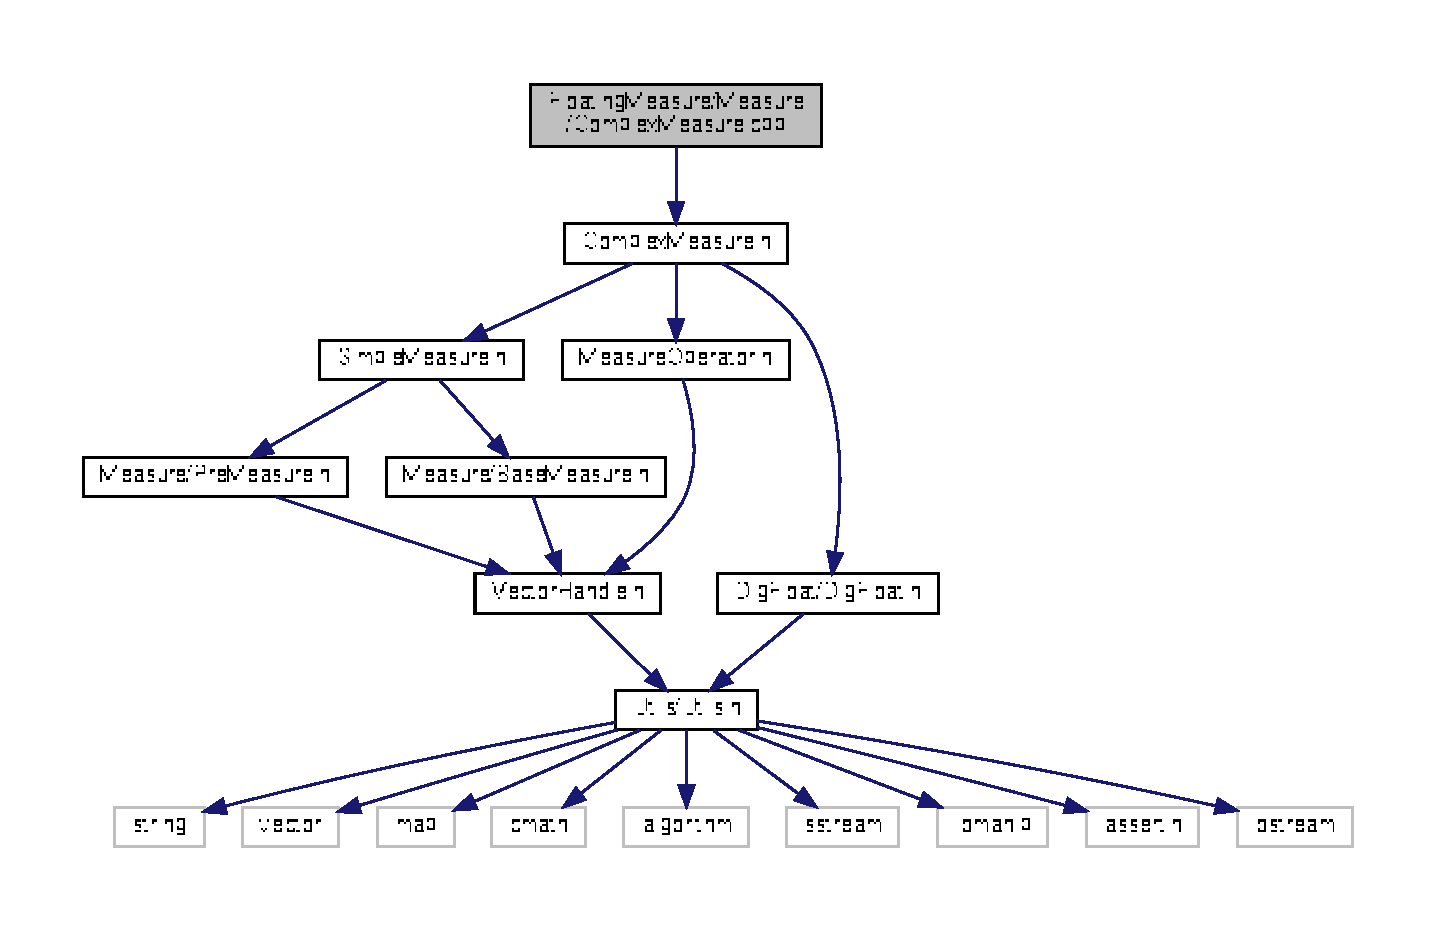
\includegraphics[width=350pt]{d0/d5a/ComplexMeasure_8cpp__incl}
\end{center}
\end{figure}

\hypertarget{ComplexMeasure_8h}{}\section{Floating\+Measure/\+Measure/\+Complex\+Measure.h File Reference}
\label{ComplexMeasure_8h}\index{Floating\+Measure/\+Measure/\+Complex\+Measure.\+h@{Floating\+Measure/\+Measure/\+Complex\+Measure.\+h}}
{\ttfamily \#include \char`\"{}Simple\+Measure.\+h\char`\"{}}\newline
{\ttfamily \#include \char`\"{}Measure\+Operator.\+h\char`\"{}}\newline
{\ttfamily \#include $<$Dig\+Float/\+Dig\+Float.\+h$>$}\newline
Include dependency graph for Complex\+Measure.\+h\+:
\nopagebreak
\begin{figure}[H]
\begin{center}
\leavevmode
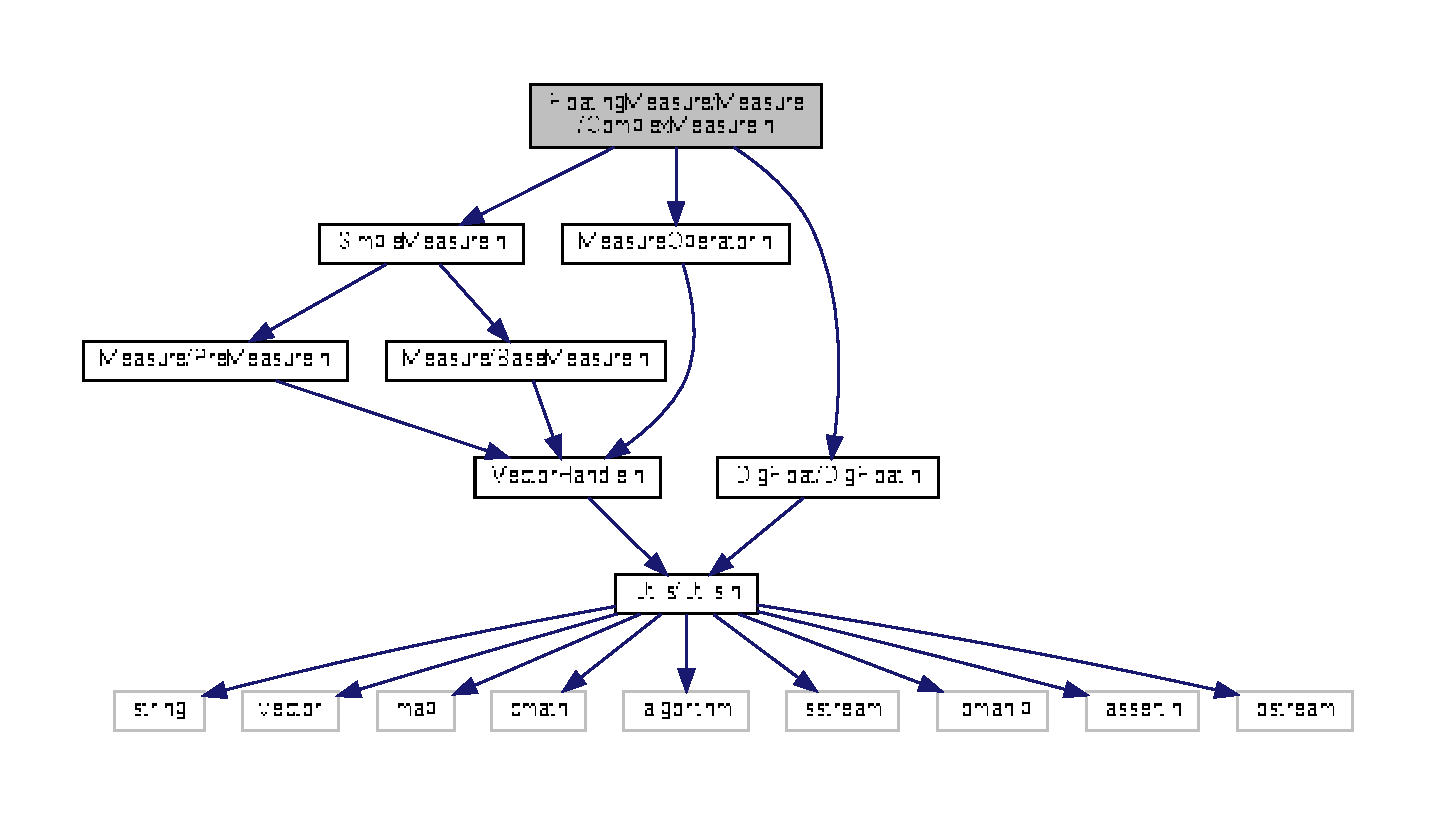
\includegraphics[width=350pt]{d0/d2f/ComplexMeasure_8h__incl}
\end{center}
\end{figure}
This graph shows which files directly or indirectly include this file\+:
\nopagebreak
\begin{figure}[H]
\begin{center}
\leavevmode
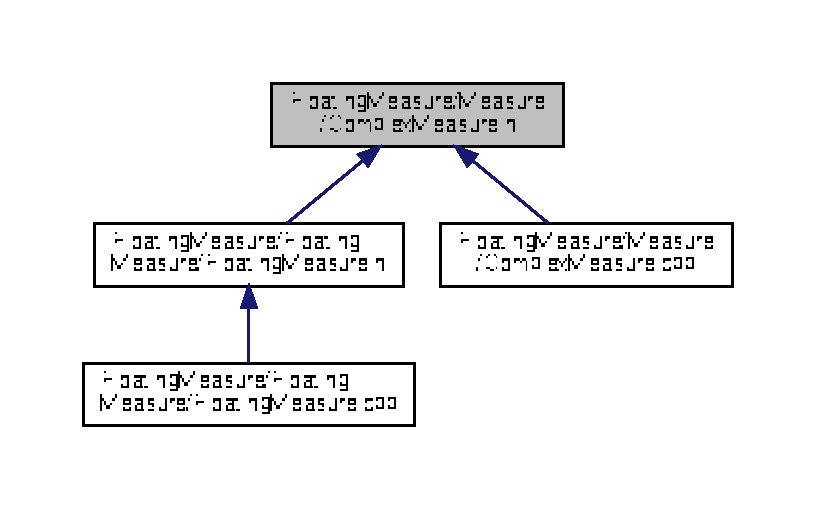
\includegraphics[width=350pt]{d5/d28/ComplexMeasure_8h__dep__incl}
\end{center}
\end{figure}
\subsection*{Classes}
\begin{DoxyCompactItemize}
\item 
class \hyperlink{classCComplexMeasure}{C\+Complex\+Measure}
\begin{DoxyCompactList}\small\item\em \hyperlink{classCComplexMeasure}{C\+Complex\+Measure}\+: represents a list of measures (i.\+e. \hyperlink{classCSimpleMeasure}{C\+Simple\+Measure}) chained by operators $\ast$ and / ~\newline
 This class handles\+: \end{DoxyCompactList}\end{DoxyCompactItemize}

\hypertarget{ComplexMeasureMacros_8h}{}\section{Floating\+Measure/\+Measure/\+Complex\+Measure\+Macros.h File Reference}
\label{ComplexMeasureMacros_8h}\index{Floating\+Measure/\+Measure/\+Complex\+Measure\+Macros.\+h@{Floating\+Measure/\+Measure/\+Complex\+Measure\+Macros.\+h}}
\subsection*{Macros}
\begin{DoxyCompactItemize}
\item 
\#define \hyperlink{ComplexMeasureMacros_8h_abc4625cc1df33feffc4026bc77ac0ff2}{cm\+Ident}~\hyperlink{classCComplexMeasure}{C\+Complex\+Measure}(\hyperlink{PreMeasure_8h_a6c81167b8d4c2badde42f81cb7214620a32bf0cb12587b174b949f8568c9ec0c3}{pm\+Ident},\hyperlink{BaseMeasure_8h_ac90e5164ccf1f0d648fba7e94b229a11a5c8528d80e9751805f662690f7764240}{bm\+Number})
\item 
\#define \hyperlink{ComplexMeasureMacros_8h_a3523d1577c64b888a1c54fc3e2c61f17}{fV}~\hyperlink{classCComplexMeasure}{C\+Complex\+Measure}(\hyperlink{PreMeasure_8h_a6c81167b8d4c2badde42f81cb7214620afaa8a9cf6a5dc121c52ccd6f50c3ffed}{pm\+Femto},\hyperlink{BaseMeasure_8h_ac90e5164ccf1f0d648fba7e94b229a11a662f2aa09627247b53e6f3c5cd10815e}{bm\+Volt})
\item 
\#define \hyperlink{ComplexMeasureMacros_8h_a988c8a0b5d4f35990e0cb115d985f912}{pV}~\hyperlink{classCComplexMeasure}{C\+Complex\+Measure}(\hyperlink{PreMeasure_8h_a6c81167b8d4c2badde42f81cb7214620a98d02efe76075e56d8ec6ecce1fd7e67}{pm\+Piko}, \hyperlink{BaseMeasure_8h_ac90e5164ccf1f0d648fba7e94b229a11a662f2aa09627247b53e6f3c5cd10815e}{bm\+Volt})
\item 
\#define \hyperlink{ComplexMeasureMacros_8h_a61d06668f7f7b52963a7a3d5e3bc1817}{nV}~\hyperlink{classCComplexMeasure}{C\+Complex\+Measure}(\hyperlink{PreMeasure_8h_a6c81167b8d4c2badde42f81cb7214620a97a6d10912fda5efedb5209ff94e11b2}{pm\+Nano}, \hyperlink{BaseMeasure_8h_ac90e5164ccf1f0d648fba7e94b229a11a662f2aa09627247b53e6f3c5cd10815e}{bm\+Volt})
\item 
\#define \hyperlink{ComplexMeasureMacros_8h_a50b1c908a37fa06447bf31309ba6fdd3}{uV}~\hyperlink{classCComplexMeasure}{C\+Complex\+Measure}(\hyperlink{PreMeasure_8h_a6c81167b8d4c2badde42f81cb7214620a186f37857e13cbb45bcbbb97c2c15561}{pm\+Micro},\hyperlink{BaseMeasure_8h_ac90e5164ccf1f0d648fba7e94b229a11a662f2aa09627247b53e6f3c5cd10815e}{bm\+Volt})
\item 
\#define \hyperlink{ComplexMeasureMacros_8h_a960d52647cdd9fc30a40b70d0e205c44}{mV}~\hyperlink{classCComplexMeasure}{C\+Complex\+Measure}(\hyperlink{PreMeasure_8h_a6c81167b8d4c2badde42f81cb7214620aff93812e5c2f401cb10fe430a1d341f4}{pm\+Milli},\hyperlink{BaseMeasure_8h_ac90e5164ccf1f0d648fba7e94b229a11a662f2aa09627247b53e6f3c5cd10815e}{bm\+Volt})
\item 
\#define \hyperlink{ComplexMeasureMacros_8h_ab9b65b55682c9f916429d8c50d4754a5}{cV}~\hyperlink{classCComplexMeasure}{C\+Complex\+Measure}(\hyperlink{PreMeasure_8h_a6c81167b8d4c2badde42f81cb7214620af7eea43f9cd732ef8e43005aeb46f0f3}{pm\+Centi},\hyperlink{BaseMeasure_8h_ac90e5164ccf1f0d648fba7e94b229a11a662f2aa09627247b53e6f3c5cd10815e}{bm\+Volt})
\item 
\#define \hyperlink{ComplexMeasureMacros_8h_a7800eb651d1910ad1f711a75846cee5e}{dV}~\hyperlink{classCComplexMeasure}{C\+Complex\+Measure}(\hyperlink{PreMeasure_8h_a6c81167b8d4c2badde42f81cb7214620a1266f4c6263ccd31d9f853fb3993e7b2}{pm\+Deci}, \hyperlink{BaseMeasure_8h_ac90e5164ccf1f0d648fba7e94b229a11a662f2aa09627247b53e6f3c5cd10815e}{bm\+Volt})
\item 
\#define \hyperlink{ComplexMeasureMacros_8h_af40a326b23c68a27cebe60f16634a2cb}{V}~\hyperlink{classCComplexMeasure}{C\+Complex\+Measure}(\hyperlink{PreMeasure_8h_a6c81167b8d4c2badde42f81cb7214620a32bf0cb12587b174b949f8568c9ec0c3}{pm\+Ident},\hyperlink{BaseMeasure_8h_ac90e5164ccf1f0d648fba7e94b229a11a662f2aa09627247b53e6f3c5cd10815e}{bm\+Volt})
\item 
\#define \hyperlink{ComplexMeasureMacros_8h_a62072af01108887668fd5642a676305f}{daV}~\hyperlink{classCComplexMeasure}{C\+Complex\+Measure}(\hyperlink{PreMeasure_8h_a6c81167b8d4c2badde42f81cb7214620a11d938995c9d37cb2b34f454cb5b3f2c}{pm\+Deca}, \hyperlink{BaseMeasure_8h_ac90e5164ccf1f0d648fba7e94b229a11a662f2aa09627247b53e6f3c5cd10815e}{bm\+Volt})
\item 
\#define \hyperlink{ComplexMeasureMacros_8h_a29d08069a1a2aa0069dd05b009e35a3d}{HV}~\hyperlink{classCComplexMeasure}{C\+Complex\+Measure}(\hyperlink{PreMeasure_8h_a6c81167b8d4c2badde42f81cb7214620ade3242e2b12643a93f3849785691d86c}{pm\+Hecto},\hyperlink{BaseMeasure_8h_ac90e5164ccf1f0d648fba7e94b229a11a662f2aa09627247b53e6f3c5cd10815e}{bm\+Volt})
\item 
\#define \hyperlink{ComplexMeasureMacros_8h_ae0a8a5de3d5e14aad79782f885bfdfe8}{kV}~\hyperlink{classCComplexMeasure}{C\+Complex\+Measure}(\hyperlink{PreMeasure_8h_a6c81167b8d4c2badde42f81cb7214620acdf63dcd9d24a1d774d2fe923621ca69}{pm\+Kilo}, \hyperlink{BaseMeasure_8h_ac90e5164ccf1f0d648fba7e94b229a11a662f2aa09627247b53e6f3c5cd10815e}{bm\+Volt})
\item 
\#define \hyperlink{ComplexMeasureMacros_8h_a7ad7aedf370a8b5c9fe4725394028f6e}{MV}~\hyperlink{classCComplexMeasure}{C\+Complex\+Measure}(\hyperlink{PreMeasure_8h_a6c81167b8d4c2badde42f81cb7214620ac669ac8a067bd6491c426c00af19f085}{pm\+Mega}, \hyperlink{BaseMeasure_8h_ac90e5164ccf1f0d648fba7e94b229a11a662f2aa09627247b53e6f3c5cd10815e}{bm\+Volt})
\item 
\#define \hyperlink{ComplexMeasureMacros_8h_ad5afb0df8a8a9e97197b4a9de8ce95cf}{GV}~\hyperlink{classCComplexMeasure}{C\+Complex\+Measure}(\hyperlink{PreMeasure_8h_a6c81167b8d4c2badde42f81cb7214620a0d6643b3b85f89178a09db0897ef502c}{pm\+Giga}, \hyperlink{BaseMeasure_8h_ac90e5164ccf1f0d648fba7e94b229a11a662f2aa09627247b53e6f3c5cd10815e}{bm\+Volt})
\item 
\#define \hyperlink{ComplexMeasureMacros_8h_a497452ebe35dad4f54b5a15343290b63}{TV}~\hyperlink{classCComplexMeasure}{C\+Complex\+Measure}(\hyperlink{PreMeasure_8h_a6c81167b8d4c2badde42f81cb7214620a70676cd51c6e17853f7cad277f473afd}{pm\+Tera}, \hyperlink{BaseMeasure_8h_ac90e5164ccf1f0d648fba7e94b229a11a662f2aa09627247b53e6f3c5cd10815e}{bm\+Volt})
\item 
\#define \hyperlink{ComplexMeasureMacros_8h_a46b90e99485a21a2150e424cc2a4afba}{PV}~\hyperlink{classCComplexMeasure}{C\+Complex\+Measure}(\hyperlink{PreMeasure_8h_a6c81167b8d4c2badde42f81cb7214620add0b3a1d027f070cedc49b5193daebba}{pm\+Peta}, \hyperlink{BaseMeasure_8h_ac90e5164ccf1f0d648fba7e94b229a11a662f2aa09627247b53e6f3c5cd10815e}{bm\+Volt})
\item 
\#define \hyperlink{ComplexMeasureMacros_8h_a650ef3eff8a2900bef69dae29c05d2dd}{EV}~\hyperlink{classCComplexMeasure}{C\+Complex\+Measure}(\hyperlink{PreMeasure_8h_a6c81167b8d4c2badde42f81cb7214620abe0b5d6c4697d04c36b1425a519fc128}{pm\+Exa},  \hyperlink{BaseMeasure_8h_ac90e5164ccf1f0d648fba7e94b229a11a662f2aa09627247b53e6f3c5cd10815e}{bm\+Volt})
\item 
\#define \hyperlink{ComplexMeasureMacros_8h_ad7d05d2245925f6a8899a085cc1138b4}{ZV}~\hyperlink{classCComplexMeasure}{C\+Complex\+Measure}(\hyperlink{PreMeasure_8h_a6c81167b8d4c2badde42f81cb7214620a00b29f37d368d66abc95fee7ecf9a034}{pm\+Zetta},\hyperlink{BaseMeasure_8h_ac90e5164ccf1f0d648fba7e94b229a11a662f2aa09627247b53e6f3c5cd10815e}{bm\+Volt})
\item 
\#define \hyperlink{ComplexMeasureMacros_8h_a0e3e7bd5ee9d05ff173d9ad8fcefe1ef}{YV}~\hyperlink{classCComplexMeasure}{C\+Complex\+Measure}(\hyperlink{PreMeasure_8h_a6c81167b8d4c2badde42f81cb7214620a5481dc587dbf4b25ddec4d4aed8e2ccb}{pm\+Yotta},\hyperlink{BaseMeasure_8h_ac90e5164ccf1f0d648fba7e94b229a11a662f2aa09627247b53e6f3c5cd10815e}{bm\+Volt})
\item 
\#define \hyperlink{ComplexMeasureMacros_8h_ad9e61764f9ba07ce30a7121f90a32354}{fA}~\hyperlink{classCComplexMeasure}{C\+Complex\+Measure}(\hyperlink{PreMeasure_8h_a6c81167b8d4c2badde42f81cb7214620afaa8a9cf6a5dc121c52ccd6f50c3ffed}{pm\+Femto},\hyperlink{BaseMeasure_8h_ac90e5164ccf1f0d648fba7e94b229a11aa0bfa4e97216cd5d37576ed9c7124f37}{bm\+Ampere})
\item 
\#define \hyperlink{ComplexMeasureMacros_8h_a166cc8406becb925e56e7e43ab4faaef}{pA}~\hyperlink{classCComplexMeasure}{C\+Complex\+Measure}(\hyperlink{PreMeasure_8h_a6c81167b8d4c2badde42f81cb7214620a98d02efe76075e56d8ec6ecce1fd7e67}{pm\+Piko}, \hyperlink{BaseMeasure_8h_ac90e5164ccf1f0d648fba7e94b229a11aa0bfa4e97216cd5d37576ed9c7124f37}{bm\+Ampere})
\item 
\#define \hyperlink{ComplexMeasureMacros_8h_aea2eef32d41eb85006a6286e76fc704c}{nA}~\hyperlink{classCComplexMeasure}{C\+Complex\+Measure}(\hyperlink{PreMeasure_8h_a6c81167b8d4c2badde42f81cb7214620a97a6d10912fda5efedb5209ff94e11b2}{pm\+Nano}, \hyperlink{BaseMeasure_8h_ac90e5164ccf1f0d648fba7e94b229a11aa0bfa4e97216cd5d37576ed9c7124f37}{bm\+Ampere})
\item 
\#define \hyperlink{ComplexMeasureMacros_8h_a9653ba133f1b6ad868c46038a7262e49}{uA}~\hyperlink{classCComplexMeasure}{C\+Complex\+Measure}(\hyperlink{PreMeasure_8h_a6c81167b8d4c2badde42f81cb7214620a186f37857e13cbb45bcbbb97c2c15561}{pm\+Micro},\hyperlink{BaseMeasure_8h_ac90e5164ccf1f0d648fba7e94b229a11aa0bfa4e97216cd5d37576ed9c7124f37}{bm\+Ampere})
\item 
\#define \hyperlink{ComplexMeasureMacros_8h_a12fc82329d8ebacab6ace2d7e2c2110e}{mA}~\hyperlink{classCComplexMeasure}{C\+Complex\+Measure}(\hyperlink{PreMeasure_8h_a6c81167b8d4c2badde42f81cb7214620aff93812e5c2f401cb10fe430a1d341f4}{pm\+Milli},\hyperlink{BaseMeasure_8h_ac90e5164ccf1f0d648fba7e94b229a11aa0bfa4e97216cd5d37576ed9c7124f37}{bm\+Ampere})
\item 
\#define \hyperlink{ComplexMeasureMacros_8h_ac924fecb3396d96721773a2fe124a221}{cA}~\hyperlink{classCComplexMeasure}{C\+Complex\+Measure}(\hyperlink{PreMeasure_8h_a6c81167b8d4c2badde42f81cb7214620af7eea43f9cd732ef8e43005aeb46f0f3}{pm\+Centi},\hyperlink{BaseMeasure_8h_ac90e5164ccf1f0d648fba7e94b229a11aa0bfa4e97216cd5d37576ed9c7124f37}{bm\+Ampere})
\item 
\#define \hyperlink{ComplexMeasureMacros_8h_a0e3cd3b65988caa08f1c550f3d30b28c}{dA}~\hyperlink{classCComplexMeasure}{C\+Complex\+Measure}(\hyperlink{PreMeasure_8h_a6c81167b8d4c2badde42f81cb7214620a1266f4c6263ccd31d9f853fb3993e7b2}{pm\+Deci}, \hyperlink{BaseMeasure_8h_ac90e5164ccf1f0d648fba7e94b229a11aa0bfa4e97216cd5d37576ed9c7124f37}{bm\+Ampere})
\item 
\#define \hyperlink{ComplexMeasureMacros_8h_a955f504eccf76b4eb2489c0adab03121}{A}~\hyperlink{classCComplexMeasure}{C\+Complex\+Measure}(\hyperlink{PreMeasure_8h_a6c81167b8d4c2badde42f81cb7214620a32bf0cb12587b174b949f8568c9ec0c3}{pm\+Ident},\hyperlink{BaseMeasure_8h_ac90e5164ccf1f0d648fba7e94b229a11aa0bfa4e97216cd5d37576ed9c7124f37}{bm\+Ampere})
\item 
\#define \hyperlink{ComplexMeasureMacros_8h_a9edfe52478a8f6788d14b0a513843401}{daA}~\hyperlink{classCComplexMeasure}{C\+Complex\+Measure}(\hyperlink{PreMeasure_8h_a6c81167b8d4c2badde42f81cb7214620a11d938995c9d37cb2b34f454cb5b3f2c}{pm\+Deca}, \hyperlink{BaseMeasure_8h_ac90e5164ccf1f0d648fba7e94b229a11aa0bfa4e97216cd5d37576ed9c7124f37}{bm\+Ampere})
\item 
\#define \hyperlink{ComplexMeasureMacros_8h_a1309e503ca21222feab2e21b4287b676}{HA}~\hyperlink{classCComplexMeasure}{C\+Complex\+Measure}(\hyperlink{PreMeasure_8h_a6c81167b8d4c2badde42f81cb7214620ade3242e2b12643a93f3849785691d86c}{pm\+Hecto},\hyperlink{BaseMeasure_8h_ac90e5164ccf1f0d648fba7e94b229a11aa0bfa4e97216cd5d37576ed9c7124f37}{bm\+Ampere})
\item 
\#define \hyperlink{ComplexMeasureMacros_8h_a407f28b550f521b082e54837e9699101}{kA}~\hyperlink{classCComplexMeasure}{C\+Complex\+Measure}(\hyperlink{PreMeasure_8h_a6c81167b8d4c2badde42f81cb7214620acdf63dcd9d24a1d774d2fe923621ca69}{pm\+Kilo}, \hyperlink{BaseMeasure_8h_ac90e5164ccf1f0d648fba7e94b229a11aa0bfa4e97216cd5d37576ed9c7124f37}{bm\+Ampere})
\item 
\#define \hyperlink{ComplexMeasureMacros_8h_a11702dcb3f3ec928229185eb96686127}{MA}~\hyperlink{classCComplexMeasure}{C\+Complex\+Measure}(\hyperlink{PreMeasure_8h_a6c81167b8d4c2badde42f81cb7214620ac669ac8a067bd6491c426c00af19f085}{pm\+Mega}, \hyperlink{BaseMeasure_8h_ac90e5164ccf1f0d648fba7e94b229a11aa0bfa4e97216cd5d37576ed9c7124f37}{bm\+Ampere})
\item 
\#define \hyperlink{ComplexMeasureMacros_8h_aee72d049d05c4a0b3b152799d34667b4}{GA}~\hyperlink{classCComplexMeasure}{C\+Complex\+Measure}(\hyperlink{PreMeasure_8h_a6c81167b8d4c2badde42f81cb7214620a0d6643b3b85f89178a09db0897ef502c}{pm\+Giga}, \hyperlink{BaseMeasure_8h_ac90e5164ccf1f0d648fba7e94b229a11aa0bfa4e97216cd5d37576ed9c7124f37}{bm\+Ampere})
\item 
\#define \hyperlink{ComplexMeasureMacros_8h_aad6d8c602d902fd4faad756ae93a52c8}{TA}~\hyperlink{classCComplexMeasure}{C\+Complex\+Measure}(\hyperlink{PreMeasure_8h_a6c81167b8d4c2badde42f81cb7214620a70676cd51c6e17853f7cad277f473afd}{pm\+Tera}, \hyperlink{BaseMeasure_8h_ac90e5164ccf1f0d648fba7e94b229a11aa0bfa4e97216cd5d37576ed9c7124f37}{bm\+Ampere})
\item 
\#define \hyperlink{ComplexMeasureMacros_8h_a74cb3af6041b109c53743b600ebbcf4c}{PA}~\hyperlink{classCComplexMeasure}{C\+Complex\+Measure}(\hyperlink{PreMeasure_8h_a6c81167b8d4c2badde42f81cb7214620add0b3a1d027f070cedc49b5193daebba}{pm\+Peta}, \hyperlink{BaseMeasure_8h_ac90e5164ccf1f0d648fba7e94b229a11aa0bfa4e97216cd5d37576ed9c7124f37}{bm\+Ampere})
\item 
\#define \hyperlink{ComplexMeasureMacros_8h_a01b31610d06aaa6316836f2c04d652e0}{EA}~\hyperlink{classCComplexMeasure}{C\+Complex\+Measure}(\hyperlink{PreMeasure_8h_a6c81167b8d4c2badde42f81cb7214620abe0b5d6c4697d04c36b1425a519fc128}{pm\+Exa},  \hyperlink{BaseMeasure_8h_ac90e5164ccf1f0d648fba7e94b229a11aa0bfa4e97216cd5d37576ed9c7124f37}{bm\+Ampere})
\item 
\#define \hyperlink{ComplexMeasureMacros_8h_a75f6618583d20d5ed1ab4262df6a11a9}{ZA}~\hyperlink{classCComplexMeasure}{C\+Complex\+Measure}(\hyperlink{PreMeasure_8h_a6c81167b8d4c2badde42f81cb7214620a00b29f37d368d66abc95fee7ecf9a034}{pm\+Zetta},\hyperlink{BaseMeasure_8h_ac90e5164ccf1f0d648fba7e94b229a11aa0bfa4e97216cd5d37576ed9c7124f37}{bm\+Ampere})
\item 
\#define \hyperlink{ComplexMeasureMacros_8h_abac2e561c296bc07ab558d595d7d9be8}{YA}~\hyperlink{classCComplexMeasure}{C\+Complex\+Measure}(\hyperlink{PreMeasure_8h_a6c81167b8d4c2badde42f81cb7214620a5481dc587dbf4b25ddec4d4aed8e2ccb}{pm\+Yotta},\hyperlink{BaseMeasure_8h_ac90e5164ccf1f0d648fba7e94b229a11aa0bfa4e97216cd5d37576ed9c7124f37}{bm\+Ampere})
\item 
\#define \hyperlink{ComplexMeasureMacros_8h_a2f72408aea32e6d1285f8af599914849}{fs}~\hyperlink{classCComplexMeasure}{C\+Complex\+Measure}(\hyperlink{PreMeasure_8h_a6c81167b8d4c2badde42f81cb7214620afaa8a9cf6a5dc121c52ccd6f50c3ffed}{pm\+Femto},\hyperlink{BaseMeasure_8h_ac90e5164ccf1f0d648fba7e94b229a11a154cadadef2b87dabd57e216a5e01f08}{bm\+Second})
\item 
\#define \hyperlink{ComplexMeasureMacros_8h_aadf956dacbac3f9d45fb3f7787bf21c1}{ps}~\hyperlink{classCComplexMeasure}{C\+Complex\+Measure}(\hyperlink{PreMeasure_8h_a6c81167b8d4c2badde42f81cb7214620a98d02efe76075e56d8ec6ecce1fd7e67}{pm\+Piko}, \hyperlink{BaseMeasure_8h_ac90e5164ccf1f0d648fba7e94b229a11a154cadadef2b87dabd57e216a5e01f08}{bm\+Second})
\item 
\#define \hyperlink{ComplexMeasureMacros_8h_ab269c6a72273579c35715ec77b41b634}{ns}~\hyperlink{classCComplexMeasure}{C\+Complex\+Measure}(\hyperlink{PreMeasure_8h_a6c81167b8d4c2badde42f81cb7214620a97a6d10912fda5efedb5209ff94e11b2}{pm\+Nano}, \hyperlink{BaseMeasure_8h_ac90e5164ccf1f0d648fba7e94b229a11a154cadadef2b87dabd57e216a5e01f08}{bm\+Second})
\item 
\#define \hyperlink{ComplexMeasureMacros_8h_a8f43d6fadb92255e98293c05b8ebd660}{us}~\hyperlink{classCComplexMeasure}{C\+Complex\+Measure}(\hyperlink{PreMeasure_8h_a6c81167b8d4c2badde42f81cb7214620a186f37857e13cbb45bcbbb97c2c15561}{pm\+Micro},\hyperlink{BaseMeasure_8h_ac90e5164ccf1f0d648fba7e94b229a11a154cadadef2b87dabd57e216a5e01f08}{bm\+Second})
\item 
\#define \hyperlink{ComplexMeasureMacros_8h_a5da6ad7b4fff3e847f96aef2f7e8db39}{ms}~\hyperlink{classCComplexMeasure}{C\+Complex\+Measure}(\hyperlink{PreMeasure_8h_a6c81167b8d4c2badde42f81cb7214620aff93812e5c2f401cb10fe430a1d341f4}{pm\+Milli},\hyperlink{BaseMeasure_8h_ac90e5164ccf1f0d648fba7e94b229a11a154cadadef2b87dabd57e216a5e01f08}{bm\+Second})
\item 
\#define \hyperlink{ComplexMeasureMacros_8h_aba8902900fa07ff44dbb4a739c0e5163}{cs}~\hyperlink{classCComplexMeasure}{C\+Complex\+Measure}(\hyperlink{PreMeasure_8h_a6c81167b8d4c2badde42f81cb7214620af7eea43f9cd732ef8e43005aeb46f0f3}{pm\+Centi},\hyperlink{BaseMeasure_8h_ac90e5164ccf1f0d648fba7e94b229a11a154cadadef2b87dabd57e216a5e01f08}{bm\+Second})
\item 
\#define \hyperlink{ComplexMeasureMacros_8h_a8a8ce01678edf9f4ecc1ea5382a1834d}{ds}~\hyperlink{classCComplexMeasure}{C\+Complex\+Measure}(\hyperlink{PreMeasure_8h_a6c81167b8d4c2badde42f81cb7214620a1266f4c6263ccd31d9f853fb3993e7b2}{pm\+Deci}, \hyperlink{BaseMeasure_8h_ac90e5164ccf1f0d648fba7e94b229a11a154cadadef2b87dabd57e216a5e01f08}{bm\+Second})
\item 
\#define \hyperlink{ComplexMeasureMacros_8h_ac9562ee4ecb3b8aeebeb04656e7e57a9}{s}~\hyperlink{classCComplexMeasure}{C\+Complex\+Measure}(\hyperlink{PreMeasure_8h_a6c81167b8d4c2badde42f81cb7214620a32bf0cb12587b174b949f8568c9ec0c3}{pm\+Ident},\hyperlink{BaseMeasure_8h_ac90e5164ccf1f0d648fba7e94b229a11a154cadadef2b87dabd57e216a5e01f08}{bm\+Second})
\item 
\#define \hyperlink{ComplexMeasureMacros_8h_a3f95963f799d461122942fb128fdbac3}{das}~\hyperlink{classCComplexMeasure}{C\+Complex\+Measure}(\hyperlink{PreMeasure_8h_a6c81167b8d4c2badde42f81cb7214620a11d938995c9d37cb2b34f454cb5b3f2c}{pm\+Deca}, \hyperlink{BaseMeasure_8h_ac90e5164ccf1f0d648fba7e94b229a11a154cadadef2b87dabd57e216a5e01f08}{bm\+Second})
\item 
\#define \hyperlink{ComplexMeasureMacros_8h_a5d1bdd06bd7f07a1f8d0f69c1ed383d9}{Hs}~\hyperlink{classCComplexMeasure}{C\+Complex\+Measure}(\hyperlink{PreMeasure_8h_a6c81167b8d4c2badde42f81cb7214620ade3242e2b12643a93f3849785691d86c}{pm\+Hecto},\hyperlink{BaseMeasure_8h_ac90e5164ccf1f0d648fba7e94b229a11a154cadadef2b87dabd57e216a5e01f08}{bm\+Second})
\item 
\#define \hyperlink{ComplexMeasureMacros_8h_a19cca36cc7785195d65e850e688e7426}{ks}~\hyperlink{classCComplexMeasure}{C\+Complex\+Measure}(\hyperlink{PreMeasure_8h_a6c81167b8d4c2badde42f81cb7214620acdf63dcd9d24a1d774d2fe923621ca69}{pm\+Kilo}, \hyperlink{BaseMeasure_8h_ac90e5164ccf1f0d648fba7e94b229a11a154cadadef2b87dabd57e216a5e01f08}{bm\+Second})
\item 
\#define \hyperlink{ComplexMeasureMacros_8h_ab0c3d2bba4f18d52d51a1216470ff304}{Ms}~\hyperlink{classCComplexMeasure}{C\+Complex\+Measure}(\hyperlink{PreMeasure_8h_a6c81167b8d4c2badde42f81cb7214620ac669ac8a067bd6491c426c00af19f085}{pm\+Mega}, \hyperlink{BaseMeasure_8h_ac90e5164ccf1f0d648fba7e94b229a11a154cadadef2b87dabd57e216a5e01f08}{bm\+Second})
\item 
\#define \hyperlink{ComplexMeasureMacros_8h_aea8e601a2f98dc8e7aa09511ee402b5b}{Gs}~\hyperlink{classCComplexMeasure}{C\+Complex\+Measure}(\hyperlink{PreMeasure_8h_a6c81167b8d4c2badde42f81cb7214620a0d6643b3b85f89178a09db0897ef502c}{pm\+Giga}, \hyperlink{BaseMeasure_8h_ac90e5164ccf1f0d648fba7e94b229a11a154cadadef2b87dabd57e216a5e01f08}{bm\+Second})
\item 
\#define \hyperlink{ComplexMeasureMacros_8h_ac271f2ecf44740ce9bc6f97396a74944}{Ts}~\hyperlink{classCComplexMeasure}{C\+Complex\+Measure}(\hyperlink{PreMeasure_8h_a6c81167b8d4c2badde42f81cb7214620a70676cd51c6e17853f7cad277f473afd}{pm\+Tera}, \hyperlink{BaseMeasure_8h_ac90e5164ccf1f0d648fba7e94b229a11a154cadadef2b87dabd57e216a5e01f08}{bm\+Second})
\item 
\#define \hyperlink{ComplexMeasureMacros_8h_a07647b74f7fef3a6d130db360133a48c}{Ps}~\hyperlink{classCComplexMeasure}{C\+Complex\+Measure}(\hyperlink{PreMeasure_8h_a6c81167b8d4c2badde42f81cb7214620add0b3a1d027f070cedc49b5193daebba}{pm\+Peta}, \hyperlink{BaseMeasure_8h_ac90e5164ccf1f0d648fba7e94b229a11a154cadadef2b87dabd57e216a5e01f08}{bm\+Second})
\item 
\#define \hyperlink{ComplexMeasureMacros_8h_a634ff02c269e4447e9579ac2b154902c}{Es}~\hyperlink{classCComplexMeasure}{C\+Complex\+Measure}(\hyperlink{PreMeasure_8h_a6c81167b8d4c2badde42f81cb7214620abe0b5d6c4697d04c36b1425a519fc128}{pm\+Exa},  \hyperlink{BaseMeasure_8h_ac90e5164ccf1f0d648fba7e94b229a11a154cadadef2b87dabd57e216a5e01f08}{bm\+Second})
\item 
\#define \hyperlink{ComplexMeasureMacros_8h_a42d713b2d5f44d037bae8ad6157333c4}{Zs}~\hyperlink{classCComplexMeasure}{C\+Complex\+Measure}(\hyperlink{PreMeasure_8h_a6c81167b8d4c2badde42f81cb7214620a00b29f37d368d66abc95fee7ecf9a034}{pm\+Zetta},\hyperlink{BaseMeasure_8h_ac90e5164ccf1f0d648fba7e94b229a11a154cadadef2b87dabd57e216a5e01f08}{bm\+Second})
\item 
\#define \hyperlink{ComplexMeasureMacros_8h_acebc4a57afe38f7080a0a1a54fc522af}{Ys}~\hyperlink{classCComplexMeasure}{C\+Complex\+Measure}(\hyperlink{PreMeasure_8h_a6c81167b8d4c2badde42f81cb7214620a5481dc587dbf4b25ddec4d4aed8e2ccb}{pm\+Yotta},\hyperlink{BaseMeasure_8h_ac90e5164ccf1f0d648fba7e94b229a11a154cadadef2b87dabd57e216a5e01f08}{bm\+Second})
\item 
\#define \hyperlink{ComplexMeasureMacros_8h_a3f06f0e9f7beb8214afeea0b18ef8377}{min}~\hyperlink{classCComplexMeasure}{C\+Complex\+Measure}(\hyperlink{PreMeasure_8h_a6c81167b8d4c2badde42f81cb7214620a32bf0cb12587b174b949f8568c9ec0c3}{pm\+Ident},\hyperlink{BaseMeasure_8h_ac90e5164ccf1f0d648fba7e94b229a11abb3a886332014c0b0b5f872651a325a3}{bm\+Minute})
\item 
\#define \hyperlink{ComplexMeasureMacros_8h_a56dee7158d9de89b23535bf5ad318261}{h}~\hyperlink{classCComplexMeasure}{C\+Complex\+Measure}(\hyperlink{PreMeasure_8h_a6c81167b8d4c2badde42f81cb7214620a32bf0cb12587b174b949f8568c9ec0c3}{pm\+Ident},\hyperlink{BaseMeasure_8h_ac90e5164ccf1f0d648fba7e94b229a11afb903ec248fbb053df2e597d3962475d}{bm\+Hour})
\item 
\#define \hyperlink{ComplexMeasureMacros_8h_a2530554172d8629149ec56816eeaa947}{d}~\hyperlink{classCComplexMeasure}{C\+Complex\+Measure}(\hyperlink{PreMeasure_8h_a6c81167b8d4c2badde42f81cb7214620a32bf0cb12587b174b949f8568c9ec0c3}{pm\+Ident},\hyperlink{BaseMeasure_8h_ac90e5164ccf1f0d648fba7e94b229a11a3b3d24fe3421db3173c33e175130c71c}{bm\+Day})
\item 
\#define \hyperlink{ComplexMeasureMacros_8h_a7a0f4d327be8132c56ccc37f2a7db6a6}{fC}~\hyperlink{classCComplexMeasure}{C\+Complex\+Measure}(\hyperlink{PreMeasure_8h_a6c81167b8d4c2badde42f81cb7214620afaa8a9cf6a5dc121c52ccd6f50c3ffed}{pm\+Femto},\hyperlink{BaseMeasure_8h_ac90e5164ccf1f0d648fba7e94b229a11a42cee40c384c9bbda9aa488151b590b4}{bm\+Deg\+Celsius})
\item 
\#define \hyperlink{ComplexMeasureMacros_8h_a2cfa7c8cffd6a972558ee9ab003dec31}{pC}~\hyperlink{classCComplexMeasure}{C\+Complex\+Measure}(\hyperlink{PreMeasure_8h_a6c81167b8d4c2badde42f81cb7214620a98d02efe76075e56d8ec6ecce1fd7e67}{pm\+Piko}, \hyperlink{BaseMeasure_8h_ac90e5164ccf1f0d648fba7e94b229a11a42cee40c384c9bbda9aa488151b590b4}{bm\+Deg\+Celsius})
\item 
\#define \hyperlink{ComplexMeasureMacros_8h_a5dbdb2848892315f476ecca7a73c5ebd}{nC}~\hyperlink{classCComplexMeasure}{C\+Complex\+Measure}(\hyperlink{PreMeasure_8h_a6c81167b8d4c2badde42f81cb7214620a97a6d10912fda5efedb5209ff94e11b2}{pm\+Nano}, \hyperlink{BaseMeasure_8h_ac90e5164ccf1f0d648fba7e94b229a11a42cee40c384c9bbda9aa488151b590b4}{bm\+Deg\+Celsius})
\item 
\#define \hyperlink{ComplexMeasureMacros_8h_abff50585ecc944205bcda8704116cab1}{uC}~\hyperlink{classCComplexMeasure}{C\+Complex\+Measure}(\hyperlink{PreMeasure_8h_a6c81167b8d4c2badde42f81cb7214620a186f37857e13cbb45bcbbb97c2c15561}{pm\+Micro},\hyperlink{BaseMeasure_8h_ac90e5164ccf1f0d648fba7e94b229a11a42cee40c384c9bbda9aa488151b590b4}{bm\+Deg\+Celsius})
\item 
\#define \hyperlink{ComplexMeasureMacros_8h_a6ddb77c3e8d7f445552b9a1eabfbf6b5}{mC}~\hyperlink{classCComplexMeasure}{C\+Complex\+Measure}(\hyperlink{PreMeasure_8h_a6c81167b8d4c2badde42f81cb7214620aff93812e5c2f401cb10fe430a1d341f4}{pm\+Milli},\hyperlink{BaseMeasure_8h_ac90e5164ccf1f0d648fba7e94b229a11a42cee40c384c9bbda9aa488151b590b4}{bm\+Deg\+Celsius})
\item 
\#define \hyperlink{ComplexMeasureMacros_8h_adfd2d4b5edc47a3dd532a5c4d8848e71}{cC}~\hyperlink{classCComplexMeasure}{C\+Complex\+Measure}(\hyperlink{PreMeasure_8h_a6c81167b8d4c2badde42f81cb7214620af7eea43f9cd732ef8e43005aeb46f0f3}{pm\+Centi},\hyperlink{BaseMeasure_8h_ac90e5164ccf1f0d648fba7e94b229a11a42cee40c384c9bbda9aa488151b590b4}{bm\+Deg\+Celsius})
\item 
\#define \hyperlink{ComplexMeasureMacros_8h_acc5ec578ced5d032234e83703b4b352a}{dC}~\hyperlink{classCComplexMeasure}{C\+Complex\+Measure}(\hyperlink{PreMeasure_8h_a6c81167b8d4c2badde42f81cb7214620a1266f4c6263ccd31d9f853fb3993e7b2}{pm\+Deci}, \hyperlink{BaseMeasure_8h_ac90e5164ccf1f0d648fba7e94b229a11a42cee40c384c9bbda9aa488151b590b4}{bm\+Deg\+Celsius})
\item 
\#define \hyperlink{ComplexMeasureMacros_8h_ac4cf4b2ab929bd23951a8676eeac086b}{C}~\hyperlink{classCComplexMeasure}{C\+Complex\+Measure}(\hyperlink{PreMeasure_8h_a6c81167b8d4c2badde42f81cb7214620a32bf0cb12587b174b949f8568c9ec0c3}{pm\+Ident},\hyperlink{BaseMeasure_8h_ac90e5164ccf1f0d648fba7e94b229a11a42cee40c384c9bbda9aa488151b590b4}{bm\+Deg\+Celsius})
\item 
\#define \hyperlink{ComplexMeasureMacros_8h_a66c6576b011d63fa2b889224a1553f2f}{daC}~\hyperlink{classCComplexMeasure}{C\+Complex\+Measure}(\hyperlink{PreMeasure_8h_a6c81167b8d4c2badde42f81cb7214620a11d938995c9d37cb2b34f454cb5b3f2c}{pm\+Deca}, \hyperlink{BaseMeasure_8h_ac90e5164ccf1f0d648fba7e94b229a11a42cee40c384c9bbda9aa488151b590b4}{bm\+Deg\+Celsius})
\item 
\#define \hyperlink{ComplexMeasureMacros_8h_a29939a749d943e3eba661f4f0302ef72}{HC}~\hyperlink{classCComplexMeasure}{C\+Complex\+Measure}(\hyperlink{PreMeasure_8h_a6c81167b8d4c2badde42f81cb7214620ade3242e2b12643a93f3849785691d86c}{pm\+Hecto},\hyperlink{BaseMeasure_8h_ac90e5164ccf1f0d648fba7e94b229a11a42cee40c384c9bbda9aa488151b590b4}{bm\+Deg\+Celsius})
\item 
\#define \hyperlink{ComplexMeasureMacros_8h_aac4b17391ba48e5680c5fdf8c1437201}{kC}~\hyperlink{classCComplexMeasure}{C\+Complex\+Measure}(\hyperlink{PreMeasure_8h_a6c81167b8d4c2badde42f81cb7214620acdf63dcd9d24a1d774d2fe923621ca69}{pm\+Kilo}, \hyperlink{BaseMeasure_8h_ac90e5164ccf1f0d648fba7e94b229a11a42cee40c384c9bbda9aa488151b590b4}{bm\+Deg\+Celsius})
\item 
\#define \hyperlink{ComplexMeasureMacros_8h_a71d9e511e7e302cd831e83581219e70d}{MC}~\hyperlink{classCComplexMeasure}{C\+Complex\+Measure}(\hyperlink{PreMeasure_8h_a6c81167b8d4c2badde42f81cb7214620ac669ac8a067bd6491c426c00af19f085}{pm\+Mega}, \hyperlink{BaseMeasure_8h_ac90e5164ccf1f0d648fba7e94b229a11a42cee40c384c9bbda9aa488151b590b4}{bm\+Deg\+Celsius})
\item 
\#define \hyperlink{ComplexMeasureMacros_8h_a17dcc767f86e6823829de8f847a5d2d4}{GC}~\hyperlink{classCComplexMeasure}{C\+Complex\+Measure}(\hyperlink{PreMeasure_8h_a6c81167b8d4c2badde42f81cb7214620a0d6643b3b85f89178a09db0897ef502c}{pm\+Giga}, \hyperlink{BaseMeasure_8h_ac90e5164ccf1f0d648fba7e94b229a11a42cee40c384c9bbda9aa488151b590b4}{bm\+Deg\+Celsius})
\item 
\#define \hyperlink{ComplexMeasureMacros_8h_ac47e5be08ceb21251f17db929ab41167}{TC}~\hyperlink{classCComplexMeasure}{C\+Complex\+Measure}(\hyperlink{PreMeasure_8h_a6c81167b8d4c2badde42f81cb7214620a70676cd51c6e17853f7cad277f473afd}{pm\+Tera}, \hyperlink{BaseMeasure_8h_ac90e5164ccf1f0d648fba7e94b229a11a42cee40c384c9bbda9aa488151b590b4}{bm\+Deg\+Celsius})
\item 
\#define \hyperlink{ComplexMeasureMacros_8h_a600721f0222b857dc8a3ae59e5077347}{PC}~\hyperlink{classCComplexMeasure}{C\+Complex\+Measure}(\hyperlink{PreMeasure_8h_a6c81167b8d4c2badde42f81cb7214620add0b3a1d027f070cedc49b5193daebba}{pm\+Peta}, \hyperlink{BaseMeasure_8h_ac90e5164ccf1f0d648fba7e94b229a11a42cee40c384c9bbda9aa488151b590b4}{bm\+Deg\+Celsius})
\item 
\#define \hyperlink{ComplexMeasureMacros_8h_a79746149dba4f3da9b7d0f09f288e782}{EC}~\hyperlink{classCComplexMeasure}{C\+Complex\+Measure}(\hyperlink{PreMeasure_8h_a6c81167b8d4c2badde42f81cb7214620abe0b5d6c4697d04c36b1425a519fc128}{pm\+Exa},  \hyperlink{BaseMeasure_8h_ac90e5164ccf1f0d648fba7e94b229a11a42cee40c384c9bbda9aa488151b590b4}{bm\+Deg\+Celsius})
\item 
\#define \hyperlink{ComplexMeasureMacros_8h_a607322f9f1d061b64bc962b8c242b354}{ZC}~\hyperlink{classCComplexMeasure}{C\+Complex\+Measure}(\hyperlink{PreMeasure_8h_a6c81167b8d4c2badde42f81cb7214620a00b29f37d368d66abc95fee7ecf9a034}{pm\+Zetta},\hyperlink{BaseMeasure_8h_ac90e5164ccf1f0d648fba7e94b229a11a42cee40c384c9bbda9aa488151b590b4}{bm\+Deg\+Celsius})
\item 
\#define \hyperlink{ComplexMeasureMacros_8h_a0b35e36ed0c7acf64cc63eebb3160d7a}{YC}~\hyperlink{classCComplexMeasure}{C\+Complex\+Measure}(\hyperlink{PreMeasure_8h_a6c81167b8d4c2badde42f81cb7214620a5481dc587dbf4b25ddec4d4aed8e2ccb}{pm\+Yotta},\hyperlink{BaseMeasure_8h_ac90e5164ccf1f0d648fba7e94b229a11a42cee40c384c9bbda9aa488151b590b4}{bm\+Deg\+Celsius})
\item 
\#define \hyperlink{ComplexMeasureMacros_8h_af5ec6f213bbabe632c9d82eea1e8f919}{fF}~\hyperlink{classCComplexMeasure}{C\+Complex\+Measure}(\hyperlink{PreMeasure_8h_a6c81167b8d4c2badde42f81cb7214620afaa8a9cf6a5dc121c52ccd6f50c3ffed}{pm\+Femto},\hyperlink{BaseMeasure_8h_ac90e5164ccf1f0d648fba7e94b229a11add58e3d33a5d9459dbe3bf9d3f90777c}{bm\+Deg\+Fahrenheit})
\item 
\#define \hyperlink{ComplexMeasureMacros_8h_a253177bee303a3fa05dd3ded2a661fb8}{pF}~\hyperlink{classCComplexMeasure}{C\+Complex\+Measure}(\hyperlink{PreMeasure_8h_a6c81167b8d4c2badde42f81cb7214620a98d02efe76075e56d8ec6ecce1fd7e67}{pm\+Piko}, \hyperlink{BaseMeasure_8h_ac90e5164ccf1f0d648fba7e94b229a11add58e3d33a5d9459dbe3bf9d3f90777c}{bm\+Deg\+Fahrenheit})
\item 
\#define \hyperlink{ComplexMeasureMacros_8h_a213da80c1d3f713a974ad52b988f44b3}{nF}~\hyperlink{classCComplexMeasure}{C\+Complex\+Measure}(\hyperlink{PreMeasure_8h_a6c81167b8d4c2badde42f81cb7214620a97a6d10912fda5efedb5209ff94e11b2}{pm\+Nano}, \hyperlink{BaseMeasure_8h_ac90e5164ccf1f0d648fba7e94b229a11add58e3d33a5d9459dbe3bf9d3f90777c}{bm\+Deg\+Fahrenheit})
\item 
\#define \hyperlink{ComplexMeasureMacros_8h_ae64cd0cfe8dfb59d985a02b7e86dd710}{uF}~\hyperlink{classCComplexMeasure}{C\+Complex\+Measure}(\hyperlink{PreMeasure_8h_a6c81167b8d4c2badde42f81cb7214620a186f37857e13cbb45bcbbb97c2c15561}{pm\+Micro},\hyperlink{BaseMeasure_8h_ac90e5164ccf1f0d648fba7e94b229a11add58e3d33a5d9459dbe3bf9d3f90777c}{bm\+Deg\+Fahrenheit})
\item 
\#define \hyperlink{ComplexMeasureMacros_8h_afd1bb0856d145d6d832f0cf8b39635db}{mF}~\hyperlink{classCComplexMeasure}{C\+Complex\+Measure}(\hyperlink{PreMeasure_8h_a6c81167b8d4c2badde42f81cb7214620aff93812e5c2f401cb10fe430a1d341f4}{pm\+Milli},\hyperlink{BaseMeasure_8h_ac90e5164ccf1f0d648fba7e94b229a11add58e3d33a5d9459dbe3bf9d3f90777c}{bm\+Deg\+Fahrenheit})
\item 
\#define \hyperlink{ComplexMeasureMacros_8h_a6db8d493e8cac9bc9cd5118260b85db8}{cF}~\hyperlink{classCComplexMeasure}{C\+Complex\+Measure}(\hyperlink{PreMeasure_8h_a6c81167b8d4c2badde42f81cb7214620af7eea43f9cd732ef8e43005aeb46f0f3}{pm\+Centi},\hyperlink{BaseMeasure_8h_ac90e5164ccf1f0d648fba7e94b229a11add58e3d33a5d9459dbe3bf9d3f90777c}{bm\+Deg\+Fahrenheit})
\item 
\#define \hyperlink{ComplexMeasureMacros_8h_ab47e8c7fdab7cec27c17175c6a0b5136}{dF}~\hyperlink{classCComplexMeasure}{C\+Complex\+Measure}(\hyperlink{PreMeasure_8h_a6c81167b8d4c2badde42f81cb7214620a1266f4c6263ccd31d9f853fb3993e7b2}{pm\+Deci}, \hyperlink{BaseMeasure_8h_ac90e5164ccf1f0d648fba7e94b229a11add58e3d33a5d9459dbe3bf9d3f90777c}{bm\+Deg\+Fahrenheit})
\item 
\#define \hyperlink{ComplexMeasureMacros_8h_a42257a545daf5b7933d6e8f96adc74f2}{F}~\hyperlink{classCComplexMeasure}{C\+Complex\+Measure}(\hyperlink{PreMeasure_8h_a6c81167b8d4c2badde42f81cb7214620a32bf0cb12587b174b949f8568c9ec0c3}{pm\+Ident},\hyperlink{BaseMeasure_8h_ac90e5164ccf1f0d648fba7e94b229a11add58e3d33a5d9459dbe3bf9d3f90777c}{bm\+Deg\+Fahrenheit})
\item 
\#define \hyperlink{ComplexMeasureMacros_8h_a9e1ec9224a4b0c23bcf11e501f6a5fd6}{daF}~\hyperlink{classCComplexMeasure}{C\+Complex\+Measure}(\hyperlink{PreMeasure_8h_a6c81167b8d4c2badde42f81cb7214620a11d938995c9d37cb2b34f454cb5b3f2c}{pm\+Deca}, \hyperlink{BaseMeasure_8h_ac90e5164ccf1f0d648fba7e94b229a11add58e3d33a5d9459dbe3bf9d3f90777c}{bm\+Deg\+Fahrenheit})
\item 
\#define \hyperlink{ComplexMeasureMacros_8h_ae573698c5f41ffdb78fae41e18139903}{HF}~\hyperlink{classCComplexMeasure}{C\+Complex\+Measure}(\hyperlink{PreMeasure_8h_a6c81167b8d4c2badde42f81cb7214620ade3242e2b12643a93f3849785691d86c}{pm\+Hecto},\hyperlink{BaseMeasure_8h_ac90e5164ccf1f0d648fba7e94b229a11add58e3d33a5d9459dbe3bf9d3f90777c}{bm\+Deg\+Fahrenheit})
\item 
\#define \hyperlink{ComplexMeasureMacros_8h_a7a581c0c19d530ca6d5561cc8f86ab04}{kF}~\hyperlink{classCComplexMeasure}{C\+Complex\+Measure}(\hyperlink{PreMeasure_8h_a6c81167b8d4c2badde42f81cb7214620acdf63dcd9d24a1d774d2fe923621ca69}{pm\+Kilo}, \hyperlink{BaseMeasure_8h_ac90e5164ccf1f0d648fba7e94b229a11add58e3d33a5d9459dbe3bf9d3f90777c}{bm\+Deg\+Fahrenheit})
\item 
\#define \hyperlink{ComplexMeasureMacros_8h_a3a4e7198623f643e4a93411d693e6922}{MF}~\hyperlink{classCComplexMeasure}{C\+Complex\+Measure}(\hyperlink{PreMeasure_8h_a6c81167b8d4c2badde42f81cb7214620ac669ac8a067bd6491c426c00af19f085}{pm\+Mega}, \hyperlink{BaseMeasure_8h_ac90e5164ccf1f0d648fba7e94b229a11add58e3d33a5d9459dbe3bf9d3f90777c}{bm\+Deg\+Fahrenheit})
\item 
\#define \hyperlink{ComplexMeasureMacros_8h_abd25a5920d0e7c91c407d821f5ef102b}{GF}~\hyperlink{classCComplexMeasure}{C\+Complex\+Measure}(\hyperlink{PreMeasure_8h_a6c81167b8d4c2badde42f81cb7214620a0d6643b3b85f89178a09db0897ef502c}{pm\+Giga}, \hyperlink{BaseMeasure_8h_ac90e5164ccf1f0d648fba7e94b229a11add58e3d33a5d9459dbe3bf9d3f90777c}{bm\+Deg\+Fahrenheit})
\item 
\#define \hyperlink{ComplexMeasureMacros_8h_a1c0168a9703a05a19de4ce775acc6647}{TF}~\hyperlink{classCComplexMeasure}{C\+Complex\+Measure}(\hyperlink{PreMeasure_8h_a6c81167b8d4c2badde42f81cb7214620a70676cd51c6e17853f7cad277f473afd}{pm\+Tera}, \hyperlink{BaseMeasure_8h_ac90e5164ccf1f0d648fba7e94b229a11add58e3d33a5d9459dbe3bf9d3f90777c}{bm\+Deg\+Fahrenheit})
\item 
\#define \hyperlink{ComplexMeasureMacros_8h_aa0e278c26c25558741febfadd7216caa}{PF}~\hyperlink{classCComplexMeasure}{C\+Complex\+Measure}(\hyperlink{PreMeasure_8h_a6c81167b8d4c2badde42f81cb7214620add0b3a1d027f070cedc49b5193daebba}{pm\+Peta}, \hyperlink{BaseMeasure_8h_ac90e5164ccf1f0d648fba7e94b229a11add58e3d33a5d9459dbe3bf9d3f90777c}{bm\+Deg\+Fahrenheit})
\item 
\#define \hyperlink{ComplexMeasureMacros_8h_a7f8e920c119fd99d39c4b910204084c5}{EF}~\hyperlink{classCComplexMeasure}{C\+Complex\+Measure}(\hyperlink{PreMeasure_8h_a6c81167b8d4c2badde42f81cb7214620abe0b5d6c4697d04c36b1425a519fc128}{pm\+Exa},  \hyperlink{BaseMeasure_8h_ac90e5164ccf1f0d648fba7e94b229a11add58e3d33a5d9459dbe3bf9d3f90777c}{bm\+Deg\+Fahrenheit})
\item 
\#define \hyperlink{ComplexMeasureMacros_8h_ab4dfddb53d3b02a91b6a0429bdc10143}{ZF}~\hyperlink{classCComplexMeasure}{C\+Complex\+Measure}(\hyperlink{PreMeasure_8h_a6c81167b8d4c2badde42f81cb7214620a00b29f37d368d66abc95fee7ecf9a034}{pm\+Zetta},\hyperlink{BaseMeasure_8h_ac90e5164ccf1f0d648fba7e94b229a11add58e3d33a5d9459dbe3bf9d3f90777c}{bm\+Deg\+Fahrenheit})
\item 
\#define \hyperlink{ComplexMeasureMacros_8h_a74e1c32283ad51af7a0e774458723b22}{YF}~\hyperlink{classCComplexMeasure}{C\+Complex\+Measure}(\hyperlink{PreMeasure_8h_a6c81167b8d4c2badde42f81cb7214620a5481dc587dbf4b25ddec4d4aed8e2ccb}{pm\+Yotta},\hyperlink{BaseMeasure_8h_ac90e5164ccf1f0d648fba7e94b229a11add58e3d33a5d9459dbe3bf9d3f90777c}{bm\+Deg\+Fahrenheit})
\item 
\#define \hyperlink{ComplexMeasureMacros_8h_a53ac557a2dbe9ef3801da0ae73d8d39b}{fK}~\hyperlink{classCComplexMeasure}{C\+Complex\+Measure}(\hyperlink{PreMeasure_8h_a6c81167b8d4c2badde42f81cb7214620afaa8a9cf6a5dc121c52ccd6f50c3ffed}{pm\+Femto},\hyperlink{BaseMeasure_8h_ac90e5164ccf1f0d648fba7e94b229a11a7d519faa41d1d34d9c378cfc61254074}{bm\+Deg\+Kelvin})
\item 
\#define \hyperlink{ComplexMeasureMacros_8h_ae4de769bdfc3f18dffc52a3bdd23cec0}{pK}~\hyperlink{classCComplexMeasure}{C\+Complex\+Measure}(\hyperlink{PreMeasure_8h_a6c81167b8d4c2badde42f81cb7214620a98d02efe76075e56d8ec6ecce1fd7e67}{pm\+Piko}, \hyperlink{BaseMeasure_8h_ac90e5164ccf1f0d648fba7e94b229a11a7d519faa41d1d34d9c378cfc61254074}{bm\+Deg\+Kelvin})
\item 
\#define \hyperlink{ComplexMeasureMacros_8h_ac2560fcba656a4a617dbeae6f2622884}{nK}~\hyperlink{classCComplexMeasure}{C\+Complex\+Measure}(\hyperlink{PreMeasure_8h_a6c81167b8d4c2badde42f81cb7214620a97a6d10912fda5efedb5209ff94e11b2}{pm\+Nano}, \hyperlink{BaseMeasure_8h_ac90e5164ccf1f0d648fba7e94b229a11a7d519faa41d1d34d9c378cfc61254074}{bm\+Deg\+Kelvin})
\item 
\#define \hyperlink{ComplexMeasureMacros_8h_a9ba052f8203be3250848e191264265af}{uK}~\hyperlink{classCComplexMeasure}{C\+Complex\+Measure}(\hyperlink{PreMeasure_8h_a6c81167b8d4c2badde42f81cb7214620a186f37857e13cbb45bcbbb97c2c15561}{pm\+Micro},\hyperlink{BaseMeasure_8h_ac90e5164ccf1f0d648fba7e94b229a11a7d519faa41d1d34d9c378cfc61254074}{bm\+Deg\+Kelvin})
\item 
\#define \hyperlink{ComplexMeasureMacros_8h_a36ea5602890b1727b39be593d1b87aaf}{mK}~\hyperlink{classCComplexMeasure}{C\+Complex\+Measure}(\hyperlink{PreMeasure_8h_a6c81167b8d4c2badde42f81cb7214620aff93812e5c2f401cb10fe430a1d341f4}{pm\+Milli},\hyperlink{BaseMeasure_8h_ac90e5164ccf1f0d648fba7e94b229a11a7d519faa41d1d34d9c378cfc61254074}{bm\+Deg\+Kelvin})
\item 
\#define \hyperlink{ComplexMeasureMacros_8h_acf7c7c58676167d2c85d16a9a212ee98}{cK}~\hyperlink{classCComplexMeasure}{C\+Complex\+Measure}(\hyperlink{PreMeasure_8h_a6c81167b8d4c2badde42f81cb7214620af7eea43f9cd732ef8e43005aeb46f0f3}{pm\+Centi},\hyperlink{BaseMeasure_8h_ac90e5164ccf1f0d648fba7e94b229a11a7d519faa41d1d34d9c378cfc61254074}{bm\+Deg\+Kelvin})
\item 
\#define \hyperlink{ComplexMeasureMacros_8h_ae6b8fc2ef5ed4c495f57337d59674298}{dK}~\hyperlink{classCComplexMeasure}{C\+Complex\+Measure}(\hyperlink{PreMeasure_8h_a6c81167b8d4c2badde42f81cb7214620a1266f4c6263ccd31d9f853fb3993e7b2}{pm\+Deci}, \hyperlink{BaseMeasure_8h_ac90e5164ccf1f0d648fba7e94b229a11a7d519faa41d1d34d9c378cfc61254074}{bm\+Deg\+Kelvin})
\item 
\#define \hyperlink{ComplexMeasureMacros_8h_a97d832ae23af4f215e801e37e4f94254}{K}~\hyperlink{classCComplexMeasure}{C\+Complex\+Measure}(\hyperlink{PreMeasure_8h_a6c81167b8d4c2badde42f81cb7214620a32bf0cb12587b174b949f8568c9ec0c3}{pm\+Ident},\hyperlink{BaseMeasure_8h_ac90e5164ccf1f0d648fba7e94b229a11a7d519faa41d1d34d9c378cfc61254074}{bm\+Deg\+Kelvin})
\item 
\#define \hyperlink{ComplexMeasureMacros_8h_ad21f7d9ee2de435351b5b1f6305d9ff1}{daK}~\hyperlink{classCComplexMeasure}{C\+Complex\+Measure}(\hyperlink{PreMeasure_8h_a6c81167b8d4c2badde42f81cb7214620a11d938995c9d37cb2b34f454cb5b3f2c}{pm\+Deca}, \hyperlink{BaseMeasure_8h_ac90e5164ccf1f0d648fba7e94b229a11a7d519faa41d1d34d9c378cfc61254074}{bm\+Deg\+Kelvin})
\item 
\#define \hyperlink{ComplexMeasureMacros_8h_a33d477de6c7428b3d6662afc445c1496}{HK}~\hyperlink{classCComplexMeasure}{C\+Complex\+Measure}(\hyperlink{PreMeasure_8h_a6c81167b8d4c2badde42f81cb7214620ade3242e2b12643a93f3849785691d86c}{pm\+Hecto},\hyperlink{BaseMeasure_8h_ac90e5164ccf1f0d648fba7e94b229a11a7d519faa41d1d34d9c378cfc61254074}{bm\+Deg\+Kelvin})
\item 
\#define \hyperlink{ComplexMeasureMacros_8h_af249a591699234f7e8402faafe5efdbc}{kK}~\hyperlink{classCComplexMeasure}{C\+Complex\+Measure}(\hyperlink{PreMeasure_8h_a6c81167b8d4c2badde42f81cb7214620acdf63dcd9d24a1d774d2fe923621ca69}{pm\+Kilo}, \hyperlink{BaseMeasure_8h_ac90e5164ccf1f0d648fba7e94b229a11a7d519faa41d1d34d9c378cfc61254074}{bm\+Deg\+Kelvin})
\item 
\#define \hyperlink{ComplexMeasureMacros_8h_a4f7ad8e1644e9a80d5946b6dd827a122}{MK}~\hyperlink{classCComplexMeasure}{C\+Complex\+Measure}(\hyperlink{PreMeasure_8h_a6c81167b8d4c2badde42f81cb7214620ac669ac8a067bd6491c426c00af19f085}{pm\+Mega}, \hyperlink{BaseMeasure_8h_ac90e5164ccf1f0d648fba7e94b229a11a7d519faa41d1d34d9c378cfc61254074}{bm\+Deg\+Kelvin})
\item 
\#define \hyperlink{ComplexMeasureMacros_8h_ae5d179c0d82225aa12d8a8a9c8215a07}{GK}~\hyperlink{classCComplexMeasure}{C\+Complex\+Measure}(\hyperlink{PreMeasure_8h_a6c81167b8d4c2badde42f81cb7214620a0d6643b3b85f89178a09db0897ef502c}{pm\+Giga}, \hyperlink{BaseMeasure_8h_ac90e5164ccf1f0d648fba7e94b229a11a7d519faa41d1d34d9c378cfc61254074}{bm\+Deg\+Kelvin})
\item 
\#define \hyperlink{ComplexMeasureMacros_8h_ad72e589e37189fb1e49961335cf6d0de}{TK}~\hyperlink{classCComplexMeasure}{C\+Complex\+Measure}(\hyperlink{PreMeasure_8h_a6c81167b8d4c2badde42f81cb7214620a70676cd51c6e17853f7cad277f473afd}{pm\+Tera}, \hyperlink{BaseMeasure_8h_ac90e5164ccf1f0d648fba7e94b229a11a7d519faa41d1d34d9c378cfc61254074}{bm\+Deg\+Kelvin})
\item 
\#define \hyperlink{ComplexMeasureMacros_8h_a73d40890e57dadd6284d83d80c088833}{PK}~\hyperlink{classCComplexMeasure}{C\+Complex\+Measure}(\hyperlink{PreMeasure_8h_a6c81167b8d4c2badde42f81cb7214620add0b3a1d027f070cedc49b5193daebba}{pm\+Peta}, \hyperlink{BaseMeasure_8h_ac90e5164ccf1f0d648fba7e94b229a11a7d519faa41d1d34d9c378cfc61254074}{bm\+Deg\+Kelvin})
\item 
\#define \hyperlink{ComplexMeasureMacros_8h_a24fb2ff974ae0ce5d5fba35eea84175c}{EK}~\hyperlink{classCComplexMeasure}{C\+Complex\+Measure}(\hyperlink{PreMeasure_8h_a6c81167b8d4c2badde42f81cb7214620abe0b5d6c4697d04c36b1425a519fc128}{pm\+Exa},  \hyperlink{BaseMeasure_8h_ac90e5164ccf1f0d648fba7e94b229a11a7d519faa41d1d34d9c378cfc61254074}{bm\+Deg\+Kelvin})
\item 
\#define \hyperlink{ComplexMeasureMacros_8h_af836a03a7588ef3d22510632f722962c}{ZK}~\hyperlink{classCComplexMeasure}{C\+Complex\+Measure}(\hyperlink{PreMeasure_8h_a6c81167b8d4c2badde42f81cb7214620a00b29f37d368d66abc95fee7ecf9a034}{pm\+Zetta},\hyperlink{BaseMeasure_8h_ac90e5164ccf1f0d648fba7e94b229a11a7d519faa41d1d34d9c378cfc61254074}{bm\+Deg\+Kelvin})
\item 
\#define \hyperlink{ComplexMeasureMacros_8h_a0203ce341d6e4e5bf9ba052a9ee9da4b}{YK}~\hyperlink{classCComplexMeasure}{C\+Complex\+Measure}(\hyperlink{PreMeasure_8h_a6c81167b8d4c2badde42f81cb7214620a5481dc587dbf4b25ddec4d4aed8e2ccb}{pm\+Yotta},\hyperlink{BaseMeasure_8h_ac90e5164ccf1f0d648fba7e94b229a11a7d519faa41d1d34d9c378cfc61254074}{bm\+Deg\+Kelvin})
\item 
\#define \hyperlink{ComplexMeasureMacros_8h_a41b367db6c7a5193359f5a27054916ac}{f\+Ohm}~\hyperlink{classCComplexMeasure}{C\+Complex\+Measure}(\hyperlink{PreMeasure_8h_a6c81167b8d4c2badde42f81cb7214620afaa8a9cf6a5dc121c52ccd6f50c3ffed}{pm\+Femto},\hyperlink{BaseMeasure_8h_ac90e5164ccf1f0d648fba7e94b229a11a3c2b76106d8f5cd21cefc918b3487282}{bm\+Ohm})
\item 
\#define \hyperlink{ComplexMeasureMacros_8h_ad6a3208f4c16ca071c17e5e20a8507ce}{p\+Ohm}~\hyperlink{classCComplexMeasure}{C\+Complex\+Measure}(\hyperlink{PreMeasure_8h_a6c81167b8d4c2badde42f81cb7214620a98d02efe76075e56d8ec6ecce1fd7e67}{pm\+Piko}, \hyperlink{BaseMeasure_8h_ac90e5164ccf1f0d648fba7e94b229a11a3c2b76106d8f5cd21cefc918b3487282}{bm\+Ohm})
\item 
\#define \hyperlink{ComplexMeasureMacros_8h_a1243d49600d1c49ff8ac8c2f9af5484f}{n\+Ohm}~\hyperlink{classCComplexMeasure}{C\+Complex\+Measure}(\hyperlink{PreMeasure_8h_a6c81167b8d4c2badde42f81cb7214620a97a6d10912fda5efedb5209ff94e11b2}{pm\+Nano}, \hyperlink{BaseMeasure_8h_ac90e5164ccf1f0d648fba7e94b229a11a3c2b76106d8f5cd21cefc918b3487282}{bm\+Ohm})
\item 
\#define \hyperlink{ComplexMeasureMacros_8h_a96b1aed81bb248cb8be346150b8c0188}{u\+Ohm}~\hyperlink{classCComplexMeasure}{C\+Complex\+Measure}(\hyperlink{PreMeasure_8h_a6c81167b8d4c2badde42f81cb7214620a186f37857e13cbb45bcbbb97c2c15561}{pm\+Micro},\hyperlink{BaseMeasure_8h_ac90e5164ccf1f0d648fba7e94b229a11a3c2b76106d8f5cd21cefc918b3487282}{bm\+Ohm})
\item 
\#define \hyperlink{ComplexMeasureMacros_8h_ab8a7a04993bb0e587750626d4da9ba3d}{m\+Ohm}~\hyperlink{classCComplexMeasure}{C\+Complex\+Measure}(\hyperlink{PreMeasure_8h_a6c81167b8d4c2badde42f81cb7214620aff93812e5c2f401cb10fe430a1d341f4}{pm\+Milli},\hyperlink{BaseMeasure_8h_ac90e5164ccf1f0d648fba7e94b229a11a3c2b76106d8f5cd21cefc918b3487282}{bm\+Ohm})
\item 
\#define \hyperlink{ComplexMeasureMacros_8h_ae5b4d6f5f717c09696e9aa0418560b75}{c\+Ohm}~\hyperlink{classCComplexMeasure}{C\+Complex\+Measure}(\hyperlink{PreMeasure_8h_a6c81167b8d4c2badde42f81cb7214620af7eea43f9cd732ef8e43005aeb46f0f3}{pm\+Centi},\hyperlink{BaseMeasure_8h_ac90e5164ccf1f0d648fba7e94b229a11a3c2b76106d8f5cd21cefc918b3487282}{bm\+Ohm})
\item 
\#define \hyperlink{ComplexMeasureMacros_8h_a2c2809b5a7581f6136c0bc7fc5f1e762}{d\+Ohm}~\hyperlink{classCComplexMeasure}{C\+Complex\+Measure}(\hyperlink{PreMeasure_8h_a6c81167b8d4c2badde42f81cb7214620a1266f4c6263ccd31d9f853fb3993e7b2}{pm\+Deci}, \hyperlink{BaseMeasure_8h_ac90e5164ccf1f0d648fba7e94b229a11a3c2b76106d8f5cd21cefc918b3487282}{bm\+Ohm})
\item 
\#define \hyperlink{ComplexMeasureMacros_8h_ad5ceb9c32b0976b5a45fa4b67521ef27}{Ohm}~\hyperlink{classCComplexMeasure}{C\+Complex\+Measure}(\hyperlink{PreMeasure_8h_a6c81167b8d4c2badde42f81cb7214620a32bf0cb12587b174b949f8568c9ec0c3}{pm\+Ident},\hyperlink{BaseMeasure_8h_ac90e5164ccf1f0d648fba7e94b229a11a3c2b76106d8f5cd21cefc918b3487282}{bm\+Ohm})
\item 
\#define \hyperlink{ComplexMeasureMacros_8h_a2450c2a6e0dc64bc2261e87a15335298}{da\+Ohm}~\hyperlink{classCComplexMeasure}{C\+Complex\+Measure}(\hyperlink{PreMeasure_8h_a6c81167b8d4c2badde42f81cb7214620a11d938995c9d37cb2b34f454cb5b3f2c}{pm\+Deca}, \hyperlink{BaseMeasure_8h_ac90e5164ccf1f0d648fba7e94b229a11a3c2b76106d8f5cd21cefc918b3487282}{bm\+Ohm})
\item 
\#define \hyperlink{ComplexMeasureMacros_8h_a0123f2822a29c9e85300f1d0134654ce}{H\+Ohm}~\hyperlink{classCComplexMeasure}{C\+Complex\+Measure}(\hyperlink{PreMeasure_8h_a6c81167b8d4c2badde42f81cb7214620ade3242e2b12643a93f3849785691d86c}{pm\+Hecto},\hyperlink{BaseMeasure_8h_ac90e5164ccf1f0d648fba7e94b229a11a3c2b76106d8f5cd21cefc918b3487282}{bm\+Ohm})
\item 
\#define \hyperlink{ComplexMeasureMacros_8h_a783dd8ae14d20b60a0160359e1129ea6}{k\+Ohm}~\hyperlink{classCComplexMeasure}{C\+Complex\+Measure}(\hyperlink{PreMeasure_8h_a6c81167b8d4c2badde42f81cb7214620acdf63dcd9d24a1d774d2fe923621ca69}{pm\+Kilo}, \hyperlink{BaseMeasure_8h_ac90e5164ccf1f0d648fba7e94b229a11a3c2b76106d8f5cd21cefc918b3487282}{bm\+Ohm})
\item 
\#define \hyperlink{ComplexMeasureMacros_8h_ab70bafd467f2458b6a0b0179fc4df225}{M\+Ohm}~\hyperlink{classCComplexMeasure}{C\+Complex\+Measure}(\hyperlink{PreMeasure_8h_a6c81167b8d4c2badde42f81cb7214620ac669ac8a067bd6491c426c00af19f085}{pm\+Mega}, \hyperlink{BaseMeasure_8h_ac90e5164ccf1f0d648fba7e94b229a11a3c2b76106d8f5cd21cefc918b3487282}{bm\+Ohm})
\item 
\#define \hyperlink{ComplexMeasureMacros_8h_a3a153a274927b69d4db3d9bd936548d3}{G\+Ohm}~\hyperlink{classCComplexMeasure}{C\+Complex\+Measure}(\hyperlink{PreMeasure_8h_a6c81167b8d4c2badde42f81cb7214620a0d6643b3b85f89178a09db0897ef502c}{pm\+Giga}, \hyperlink{BaseMeasure_8h_ac90e5164ccf1f0d648fba7e94b229a11a3c2b76106d8f5cd21cefc918b3487282}{bm\+Ohm})
\item 
\#define \hyperlink{ComplexMeasureMacros_8h_a9620be1a3db0404ec58f9b67cc57e034}{T\+Ohm}~\hyperlink{classCComplexMeasure}{C\+Complex\+Measure}(\hyperlink{PreMeasure_8h_a6c81167b8d4c2badde42f81cb7214620a70676cd51c6e17853f7cad277f473afd}{pm\+Tera}, \hyperlink{BaseMeasure_8h_ac90e5164ccf1f0d648fba7e94b229a11a3c2b76106d8f5cd21cefc918b3487282}{bm\+Ohm})
\item 
\#define \hyperlink{ComplexMeasureMacros_8h_a581e259b2475b4a75fd4f59631e395f4}{P\+Ohm}~\hyperlink{classCComplexMeasure}{C\+Complex\+Measure}(\hyperlink{PreMeasure_8h_a6c81167b8d4c2badde42f81cb7214620add0b3a1d027f070cedc49b5193daebba}{pm\+Peta}, \hyperlink{BaseMeasure_8h_ac90e5164ccf1f0d648fba7e94b229a11a3c2b76106d8f5cd21cefc918b3487282}{bm\+Ohm})
\item 
\#define \hyperlink{ComplexMeasureMacros_8h_a7e326ebd0df9b5cf30c33e083d481983}{E\+Ohm}~\hyperlink{classCComplexMeasure}{C\+Complex\+Measure}(\hyperlink{PreMeasure_8h_a6c81167b8d4c2badde42f81cb7214620abe0b5d6c4697d04c36b1425a519fc128}{pm\+Exa},  \hyperlink{BaseMeasure_8h_ac90e5164ccf1f0d648fba7e94b229a11a3c2b76106d8f5cd21cefc918b3487282}{bm\+Ohm})
\item 
\#define \hyperlink{ComplexMeasureMacros_8h_a1f23a6df552802a926458be2524e33d7}{Z\+Ohm}~\hyperlink{classCComplexMeasure}{C\+Complex\+Measure}(\hyperlink{PreMeasure_8h_a6c81167b8d4c2badde42f81cb7214620a00b29f37d368d66abc95fee7ecf9a034}{pm\+Zetta},\hyperlink{BaseMeasure_8h_ac90e5164ccf1f0d648fba7e94b229a11a3c2b76106d8f5cd21cefc918b3487282}{bm\+Ohm})
\item 
\#define \hyperlink{ComplexMeasureMacros_8h_a9a97a642afe7be97717c3bf22060805e}{Y\+Ohm}~\hyperlink{classCComplexMeasure}{C\+Complex\+Measure}(\hyperlink{PreMeasure_8h_a6c81167b8d4c2badde42f81cb7214620a5481dc587dbf4b25ddec4d4aed8e2ccb}{pm\+Yotta},\hyperlink{BaseMeasure_8h_ac90e5164ccf1f0d648fba7e94b229a11a3c2b76106d8f5cd21cefc918b3487282}{bm\+Ohm})
\item 
\#define \hyperlink{ComplexMeasureMacros_8h_abec6be4093a598a34f5079446e7562a4}{f\+Hz}~\hyperlink{classCComplexMeasure}{C\+Complex\+Measure}(\hyperlink{PreMeasure_8h_a6c81167b8d4c2badde42f81cb7214620afaa8a9cf6a5dc121c52ccd6f50c3ffed}{pm\+Femto},\hyperlink{BaseMeasure_8h_ac90e5164ccf1f0d648fba7e94b229a11af98f442616dcb74a8a3af3a05c65906a}{bm\+Hertz})
\item 
\#define \hyperlink{ComplexMeasureMacros_8h_a91b19ec18024d58d57f016bd78673261}{p\+Hz}~\hyperlink{classCComplexMeasure}{C\+Complex\+Measure}(\hyperlink{PreMeasure_8h_a6c81167b8d4c2badde42f81cb7214620a98d02efe76075e56d8ec6ecce1fd7e67}{pm\+Piko}, \hyperlink{BaseMeasure_8h_ac90e5164ccf1f0d648fba7e94b229a11af98f442616dcb74a8a3af3a05c65906a}{bm\+Hertz})
\item 
\#define \hyperlink{ComplexMeasureMacros_8h_ac59b73660b35862813c912f2dfa60487}{n\+Hz}~\hyperlink{classCComplexMeasure}{C\+Complex\+Measure}(\hyperlink{PreMeasure_8h_a6c81167b8d4c2badde42f81cb7214620a97a6d10912fda5efedb5209ff94e11b2}{pm\+Nano}, \hyperlink{BaseMeasure_8h_ac90e5164ccf1f0d648fba7e94b229a11af98f442616dcb74a8a3af3a05c65906a}{bm\+Hertz})
\item 
\#define \hyperlink{ComplexMeasureMacros_8h_ab049a41a8c8b38b83b694ccce80e959c}{u\+Hz}~\hyperlink{classCComplexMeasure}{C\+Complex\+Measure}(\hyperlink{PreMeasure_8h_a6c81167b8d4c2badde42f81cb7214620a186f37857e13cbb45bcbbb97c2c15561}{pm\+Micro},\hyperlink{BaseMeasure_8h_ac90e5164ccf1f0d648fba7e94b229a11af98f442616dcb74a8a3af3a05c65906a}{bm\+Hertz})
\item 
\#define \hyperlink{ComplexMeasureMacros_8h_a801b4c08af3a607626efca32650e7cf5}{m\+Hz}~\hyperlink{classCComplexMeasure}{C\+Complex\+Measure}(\hyperlink{PreMeasure_8h_a6c81167b8d4c2badde42f81cb7214620aff93812e5c2f401cb10fe430a1d341f4}{pm\+Milli},\hyperlink{BaseMeasure_8h_ac90e5164ccf1f0d648fba7e94b229a11af98f442616dcb74a8a3af3a05c65906a}{bm\+Hertz})
\item 
\#define \hyperlink{ComplexMeasureMacros_8h_a827dba912ec2d973f241d6f4f81779f7}{c\+Hz}~\hyperlink{classCComplexMeasure}{C\+Complex\+Measure}(\hyperlink{PreMeasure_8h_a6c81167b8d4c2badde42f81cb7214620af7eea43f9cd732ef8e43005aeb46f0f3}{pm\+Centi},\hyperlink{BaseMeasure_8h_ac90e5164ccf1f0d648fba7e94b229a11af98f442616dcb74a8a3af3a05c65906a}{bm\+Hertz})
\item 
\#define \hyperlink{ComplexMeasureMacros_8h_a1e9ad1e20012dce9d36b7ad78671f1cc}{d\+Hz}~\hyperlink{classCComplexMeasure}{C\+Complex\+Measure}(\hyperlink{PreMeasure_8h_a6c81167b8d4c2badde42f81cb7214620a1266f4c6263ccd31d9f853fb3993e7b2}{pm\+Deci}, \hyperlink{BaseMeasure_8h_ac90e5164ccf1f0d648fba7e94b229a11af98f442616dcb74a8a3af3a05c65906a}{bm\+Hertz})
\item 
\#define \hyperlink{ComplexMeasureMacros_8h_a2344d042b01c5e206dc80d736560cda0}{Hz}~\hyperlink{classCComplexMeasure}{C\+Complex\+Measure}(\hyperlink{PreMeasure_8h_a6c81167b8d4c2badde42f81cb7214620a32bf0cb12587b174b949f8568c9ec0c3}{pm\+Ident},\hyperlink{BaseMeasure_8h_ac90e5164ccf1f0d648fba7e94b229a11af98f442616dcb74a8a3af3a05c65906a}{bm\+Hertz})
\item 
\#define \hyperlink{ComplexMeasureMacros_8h_a919741170e7ab01e4da7ccc6ab5d2f9e}{da\+Hz}~\hyperlink{classCComplexMeasure}{C\+Complex\+Measure}(\hyperlink{PreMeasure_8h_a6c81167b8d4c2badde42f81cb7214620a11d938995c9d37cb2b34f454cb5b3f2c}{pm\+Deca}, \hyperlink{BaseMeasure_8h_ac90e5164ccf1f0d648fba7e94b229a11af98f442616dcb74a8a3af3a05c65906a}{bm\+Hertz})
\item 
\#define \hyperlink{ComplexMeasureMacros_8h_af35daab8251857861c62c9be4ab7bbb4}{H\+Hz}~\hyperlink{classCComplexMeasure}{C\+Complex\+Measure}(\hyperlink{PreMeasure_8h_a6c81167b8d4c2badde42f81cb7214620ade3242e2b12643a93f3849785691d86c}{pm\+Hecto},\hyperlink{BaseMeasure_8h_ac90e5164ccf1f0d648fba7e94b229a11af98f442616dcb74a8a3af3a05c65906a}{bm\+Hertz})
\item 
\#define \hyperlink{ComplexMeasureMacros_8h_a599a1ece15a5eff312b9ceb732596226}{k\+Hz}~\hyperlink{classCComplexMeasure}{C\+Complex\+Measure}(\hyperlink{PreMeasure_8h_a6c81167b8d4c2badde42f81cb7214620acdf63dcd9d24a1d774d2fe923621ca69}{pm\+Kilo}, \hyperlink{BaseMeasure_8h_ac90e5164ccf1f0d648fba7e94b229a11af98f442616dcb74a8a3af3a05c65906a}{bm\+Hertz})
\item 
\#define \hyperlink{ComplexMeasureMacros_8h_a978be084da4a9180ba3bd85c0d385ce2}{M\+Hz}~\hyperlink{classCComplexMeasure}{C\+Complex\+Measure}(\hyperlink{PreMeasure_8h_a6c81167b8d4c2badde42f81cb7214620ac669ac8a067bd6491c426c00af19f085}{pm\+Mega}, \hyperlink{BaseMeasure_8h_ac90e5164ccf1f0d648fba7e94b229a11af98f442616dcb74a8a3af3a05c65906a}{bm\+Hertz})
\item 
\#define \hyperlink{ComplexMeasureMacros_8h_a307735a79741533eb11c97d364327bd3}{G\+Hz}~\hyperlink{classCComplexMeasure}{C\+Complex\+Measure}(\hyperlink{PreMeasure_8h_a6c81167b8d4c2badde42f81cb7214620a0d6643b3b85f89178a09db0897ef502c}{pm\+Giga}, \hyperlink{BaseMeasure_8h_ac90e5164ccf1f0d648fba7e94b229a11af98f442616dcb74a8a3af3a05c65906a}{bm\+Hertz})
\item 
\#define \hyperlink{ComplexMeasureMacros_8h_a602a666d18b555b91f9ffb0d1186d082}{T\+Hz}~\hyperlink{classCComplexMeasure}{C\+Complex\+Measure}(\hyperlink{PreMeasure_8h_a6c81167b8d4c2badde42f81cb7214620a70676cd51c6e17853f7cad277f473afd}{pm\+Tera}, \hyperlink{BaseMeasure_8h_ac90e5164ccf1f0d648fba7e94b229a11af98f442616dcb74a8a3af3a05c65906a}{bm\+Hertz})
\item 
\#define \hyperlink{ComplexMeasureMacros_8h_a869e810d2132204e4624c73185e0ed12}{P\+Hz}~\hyperlink{classCComplexMeasure}{C\+Complex\+Measure}(\hyperlink{PreMeasure_8h_a6c81167b8d4c2badde42f81cb7214620add0b3a1d027f070cedc49b5193daebba}{pm\+Peta}, \hyperlink{BaseMeasure_8h_ac90e5164ccf1f0d648fba7e94b229a11af98f442616dcb74a8a3af3a05c65906a}{bm\+Hertz})
\item 
\#define \hyperlink{ComplexMeasureMacros_8h_aafb3258284816cacf6dd0b96ebd23e34}{E\+Hz}~\hyperlink{classCComplexMeasure}{C\+Complex\+Measure}(\hyperlink{PreMeasure_8h_a6c81167b8d4c2badde42f81cb7214620abe0b5d6c4697d04c36b1425a519fc128}{pm\+Exa},  \hyperlink{BaseMeasure_8h_ac90e5164ccf1f0d648fba7e94b229a11af98f442616dcb74a8a3af3a05c65906a}{bm\+Hertz})
\item 
\#define \hyperlink{ComplexMeasureMacros_8h_a355ff35ada5c740d67a03385f084871f}{Z\+Hz}~\hyperlink{classCComplexMeasure}{C\+Complex\+Measure}(\hyperlink{PreMeasure_8h_a6c81167b8d4c2badde42f81cb7214620a00b29f37d368d66abc95fee7ecf9a034}{pm\+Zetta},\hyperlink{BaseMeasure_8h_ac90e5164ccf1f0d648fba7e94b229a11af98f442616dcb74a8a3af3a05c65906a}{bm\+Hertz})
\item 
\#define \hyperlink{ComplexMeasureMacros_8h_a9c8cf3f689b7960247405d2b7e3d22eb}{Y\+Hz}~\hyperlink{classCComplexMeasure}{C\+Complex\+Measure}(\hyperlink{PreMeasure_8h_a6c81167b8d4c2badde42f81cb7214620a5481dc587dbf4b25ddec4d4aed8e2ccb}{pm\+Yotta},\hyperlink{BaseMeasure_8h_ac90e5164ccf1f0d648fba7e94b229a11af98f442616dcb74a8a3af3a05c65906a}{bm\+Hertz})
\item 
\#define \hyperlink{ComplexMeasureMacros_8h_a3615cd1bfae88d6e9fbf531d1259a3a6}{fm}~\hyperlink{classCComplexMeasure}{C\+Complex\+Measure}(\hyperlink{PreMeasure_8h_a6c81167b8d4c2badde42f81cb7214620afaa8a9cf6a5dc121c52ccd6f50c3ffed}{pm\+Femto},\hyperlink{BaseMeasure_8h_ac90e5164ccf1f0d648fba7e94b229a11a648bcf7faf2a79b8e7a13e785a84295c}{bm\+Meter})
\item 
\#define \hyperlink{ComplexMeasureMacros_8h_a53e022afc9b439185fe575605b33fcbe}{pm}~\hyperlink{classCComplexMeasure}{C\+Complex\+Measure}(\hyperlink{PreMeasure_8h_a6c81167b8d4c2badde42f81cb7214620a98d02efe76075e56d8ec6ecce1fd7e67}{pm\+Piko}, \hyperlink{BaseMeasure_8h_ac90e5164ccf1f0d648fba7e94b229a11a648bcf7faf2a79b8e7a13e785a84295c}{bm\+Meter})
\item 
\#define \hyperlink{ComplexMeasureMacros_8h_a8bb34dc2a0e1adaed97d57e909212a25}{nm}~\hyperlink{classCComplexMeasure}{C\+Complex\+Measure}(\hyperlink{PreMeasure_8h_a6c81167b8d4c2badde42f81cb7214620a97a6d10912fda5efedb5209ff94e11b2}{pm\+Nano}, \hyperlink{BaseMeasure_8h_ac90e5164ccf1f0d648fba7e94b229a11a648bcf7faf2a79b8e7a13e785a84295c}{bm\+Meter})
\item 
\#define \hyperlink{ComplexMeasureMacros_8h_a6f1cf8e9872eee22fedac213c03beca0}{um}~\hyperlink{classCComplexMeasure}{C\+Complex\+Measure}(\hyperlink{PreMeasure_8h_a6c81167b8d4c2badde42f81cb7214620a186f37857e13cbb45bcbbb97c2c15561}{pm\+Micro},\hyperlink{BaseMeasure_8h_ac90e5164ccf1f0d648fba7e94b229a11a648bcf7faf2a79b8e7a13e785a84295c}{bm\+Meter})
\item 
\#define \hyperlink{ComplexMeasureMacros_8h_af9d5cb2cb2baa77a1467616b3675bd1f}{mm}~\hyperlink{classCComplexMeasure}{C\+Complex\+Measure}(\hyperlink{PreMeasure_8h_a6c81167b8d4c2badde42f81cb7214620aff93812e5c2f401cb10fe430a1d341f4}{pm\+Milli},\hyperlink{BaseMeasure_8h_ac90e5164ccf1f0d648fba7e94b229a11a648bcf7faf2a79b8e7a13e785a84295c}{bm\+Meter})
\item 
\#define \hyperlink{ComplexMeasureMacros_8h_a583257b7c70608a95289b0a109197ca3}{cm}~\hyperlink{classCComplexMeasure}{C\+Complex\+Measure}(\hyperlink{PreMeasure_8h_a6c81167b8d4c2badde42f81cb7214620af7eea43f9cd732ef8e43005aeb46f0f3}{pm\+Centi},\hyperlink{BaseMeasure_8h_ac90e5164ccf1f0d648fba7e94b229a11a648bcf7faf2a79b8e7a13e785a84295c}{bm\+Meter})
\item 
\#define \hyperlink{ComplexMeasureMacros_8h_a79ff00c9948d4542f3a68764cbe7070d}{dm}~\hyperlink{classCComplexMeasure}{C\+Complex\+Measure}(\hyperlink{PreMeasure_8h_a6c81167b8d4c2badde42f81cb7214620a1266f4c6263ccd31d9f853fb3993e7b2}{pm\+Deci}, \hyperlink{BaseMeasure_8h_ac90e5164ccf1f0d648fba7e94b229a11a648bcf7faf2a79b8e7a13e785a84295c}{bm\+Meter})
\item 
\#define \hyperlink{ComplexMeasureMacros_8h_a00626facb4f86efb8618a4c5f5c3c5f8}{m}~\hyperlink{classCComplexMeasure}{C\+Complex\+Measure}(\hyperlink{PreMeasure_8h_a6c81167b8d4c2badde42f81cb7214620a32bf0cb12587b174b949f8568c9ec0c3}{pm\+Ident},\hyperlink{BaseMeasure_8h_ac90e5164ccf1f0d648fba7e94b229a11a648bcf7faf2a79b8e7a13e785a84295c}{bm\+Meter})
\item 
\#define \hyperlink{ComplexMeasureMacros_8h_ab460be562259cd6fda02f56be31be378}{dam}~\hyperlink{classCComplexMeasure}{C\+Complex\+Measure}(\hyperlink{PreMeasure_8h_a6c81167b8d4c2badde42f81cb7214620a11d938995c9d37cb2b34f454cb5b3f2c}{pm\+Deca}, \hyperlink{BaseMeasure_8h_ac90e5164ccf1f0d648fba7e94b229a11a648bcf7faf2a79b8e7a13e785a84295c}{bm\+Meter})
\item 
\#define \hyperlink{ComplexMeasureMacros_8h_adbdaeb6e7a6e41aa8a3dc741d5bb7dd5}{Hm}~\hyperlink{classCComplexMeasure}{C\+Complex\+Measure}(\hyperlink{PreMeasure_8h_a6c81167b8d4c2badde42f81cb7214620ade3242e2b12643a93f3849785691d86c}{pm\+Hecto},\hyperlink{BaseMeasure_8h_ac90e5164ccf1f0d648fba7e94b229a11a648bcf7faf2a79b8e7a13e785a84295c}{bm\+Meter})
\item 
\#define \hyperlink{ComplexMeasureMacros_8h_a10701558a1e05f80f89e9bcd94fcbd00}{km}~\hyperlink{classCComplexMeasure}{C\+Complex\+Measure}(\hyperlink{PreMeasure_8h_a6c81167b8d4c2badde42f81cb7214620acdf63dcd9d24a1d774d2fe923621ca69}{pm\+Kilo}, \hyperlink{BaseMeasure_8h_ac90e5164ccf1f0d648fba7e94b229a11a648bcf7faf2a79b8e7a13e785a84295c}{bm\+Meter})
\item 
\#define \hyperlink{ComplexMeasureMacros_8h_a0bfb70b517f37f42e7752ee6b647f316}{Mm}~\hyperlink{classCComplexMeasure}{C\+Complex\+Measure}(\hyperlink{PreMeasure_8h_a6c81167b8d4c2badde42f81cb7214620ac669ac8a067bd6491c426c00af19f085}{pm\+Mega}, \hyperlink{BaseMeasure_8h_ac90e5164ccf1f0d648fba7e94b229a11a648bcf7faf2a79b8e7a13e785a84295c}{bm\+Meter})
\item 
\#define \hyperlink{ComplexMeasureMacros_8h_acd8f76c2e1e889ccbf6f734d0f848714}{Gm}~\hyperlink{classCComplexMeasure}{C\+Complex\+Measure}(\hyperlink{PreMeasure_8h_a6c81167b8d4c2badde42f81cb7214620a0d6643b3b85f89178a09db0897ef502c}{pm\+Giga}, \hyperlink{BaseMeasure_8h_ac90e5164ccf1f0d648fba7e94b229a11a648bcf7faf2a79b8e7a13e785a84295c}{bm\+Meter})
\item 
\#define \hyperlink{ComplexMeasureMacros_8h_a1c6dbed21310362af993884251334363}{Tm}~\hyperlink{classCComplexMeasure}{C\+Complex\+Measure}(\hyperlink{PreMeasure_8h_a6c81167b8d4c2badde42f81cb7214620a70676cd51c6e17853f7cad277f473afd}{pm\+Tera}, \hyperlink{BaseMeasure_8h_ac90e5164ccf1f0d648fba7e94b229a11a648bcf7faf2a79b8e7a13e785a84295c}{bm\+Meter})
\item 
\#define \hyperlink{ComplexMeasureMacros_8h_ac70db52ee9f04d0b3f566821f23786fc}{Pm}~\hyperlink{classCComplexMeasure}{C\+Complex\+Measure}(\hyperlink{PreMeasure_8h_a6c81167b8d4c2badde42f81cb7214620add0b3a1d027f070cedc49b5193daebba}{pm\+Peta}, \hyperlink{BaseMeasure_8h_ac90e5164ccf1f0d648fba7e94b229a11a648bcf7faf2a79b8e7a13e785a84295c}{bm\+Meter})
\item 
\#define \hyperlink{ComplexMeasureMacros_8h_ae969cf25bab0de48a547ce267c8e0d5c}{Em}~\hyperlink{classCComplexMeasure}{C\+Complex\+Measure}(\hyperlink{PreMeasure_8h_a6c81167b8d4c2badde42f81cb7214620abe0b5d6c4697d04c36b1425a519fc128}{pm\+Exa},  \hyperlink{BaseMeasure_8h_ac90e5164ccf1f0d648fba7e94b229a11a648bcf7faf2a79b8e7a13e785a84295c}{bm\+Meter})
\item 
\#define \hyperlink{ComplexMeasureMacros_8h_ac3966ba8bb7f94c5a55663293a73543f}{Zm}~\hyperlink{classCComplexMeasure}{C\+Complex\+Measure}(\hyperlink{PreMeasure_8h_a6c81167b8d4c2badde42f81cb7214620a00b29f37d368d66abc95fee7ecf9a034}{pm\+Zetta},\hyperlink{BaseMeasure_8h_ac90e5164ccf1f0d648fba7e94b229a11a648bcf7faf2a79b8e7a13e785a84295c}{bm\+Meter})
\item 
\#define \hyperlink{ComplexMeasureMacros_8h_a28eba7357d2b7cc08b02feeac652b944}{Ym}~\hyperlink{classCComplexMeasure}{C\+Complex\+Measure}(\hyperlink{PreMeasure_8h_a6c81167b8d4c2badde42f81cb7214620a5481dc587dbf4b25ddec4d4aed8e2ccb}{pm\+Yotta},\hyperlink{BaseMeasure_8h_ac90e5164ccf1f0d648fba7e94b229a11a648bcf7faf2a79b8e7a13e785a84295c}{bm\+Meter})
\end{DoxyCompactItemize}


\subsection{Macro Definition Documentation}
\mbox{\Hypertarget{ComplexMeasureMacros_8h_a955f504eccf76b4eb2489c0adab03121}\label{ComplexMeasureMacros_8h_a955f504eccf76b4eb2489c0adab03121}} 
\index{Complex\+Measure\+Macros.\+h@{Complex\+Measure\+Macros.\+h}!A@{A}}
\index{A@{A}!Complex\+Measure\+Macros.\+h@{Complex\+Measure\+Macros.\+h}}
\subsubsection{\texorpdfstring{A}{A}}
{\footnotesize\ttfamily \#define A~\hyperlink{classCComplexMeasure}{C\+Complex\+Measure}(\hyperlink{PreMeasure_8h_a6c81167b8d4c2badde42f81cb7214620a32bf0cb12587b174b949f8568c9ec0c3}{pm\+Ident},\hyperlink{BaseMeasure_8h_ac90e5164ccf1f0d648fba7e94b229a11aa0bfa4e97216cd5d37576ed9c7124f37}{bm\+Ampere})}



Definition at line 59 of file Complex\+Measure\+Macros.\+h.

\mbox{\Hypertarget{ComplexMeasureMacros_8h_ac4cf4b2ab929bd23951a8676eeac086b}\label{ComplexMeasureMacros_8h_ac4cf4b2ab929bd23951a8676eeac086b}} 
\index{Complex\+Measure\+Macros.\+h@{Complex\+Measure\+Macros.\+h}!C@{C}}
\index{C@{C}!Complex\+Measure\+Macros.\+h@{Complex\+Measure\+Macros.\+h}}
\subsubsection{\texorpdfstring{C}{C}}
{\footnotesize\ttfamily \#define C~\hyperlink{classCComplexMeasure}{C\+Complex\+Measure}(\hyperlink{PreMeasure_8h_a6c81167b8d4c2badde42f81cb7214620a32bf0cb12587b174b949f8568c9ec0c3}{pm\+Ident},\hyperlink{BaseMeasure_8h_ac90e5164ccf1f0d648fba7e94b229a11a42cee40c384c9bbda9aa488151b590b4}{bm\+Deg\+Celsius})}



Definition at line 101 of file Complex\+Measure\+Macros.\+h.

\mbox{\Hypertarget{ComplexMeasureMacros_8h_ac924fecb3396d96721773a2fe124a221}\label{ComplexMeasureMacros_8h_ac924fecb3396d96721773a2fe124a221}} 
\index{Complex\+Measure\+Macros.\+h@{Complex\+Measure\+Macros.\+h}!cA@{cA}}
\index{cA@{cA}!Complex\+Measure\+Macros.\+h@{Complex\+Measure\+Macros.\+h}}
\subsubsection{\texorpdfstring{cA}{cA}}
{\footnotesize\ttfamily \#define cA~\hyperlink{classCComplexMeasure}{C\+Complex\+Measure}(\hyperlink{PreMeasure_8h_a6c81167b8d4c2badde42f81cb7214620af7eea43f9cd732ef8e43005aeb46f0f3}{pm\+Centi},\hyperlink{BaseMeasure_8h_ac90e5164ccf1f0d648fba7e94b229a11aa0bfa4e97216cd5d37576ed9c7124f37}{bm\+Ampere})}



Definition at line 57 of file Complex\+Measure\+Macros.\+h.

\mbox{\Hypertarget{ComplexMeasureMacros_8h_adfd2d4b5edc47a3dd532a5c4d8848e71}\label{ComplexMeasureMacros_8h_adfd2d4b5edc47a3dd532a5c4d8848e71}} 
\index{Complex\+Measure\+Macros.\+h@{Complex\+Measure\+Macros.\+h}!cC@{cC}}
\index{cC@{cC}!Complex\+Measure\+Macros.\+h@{Complex\+Measure\+Macros.\+h}}
\subsubsection{\texorpdfstring{cC}{cC}}
{\footnotesize\ttfamily \#define cC~\hyperlink{classCComplexMeasure}{C\+Complex\+Measure}(\hyperlink{PreMeasure_8h_a6c81167b8d4c2badde42f81cb7214620af7eea43f9cd732ef8e43005aeb46f0f3}{pm\+Centi},\hyperlink{BaseMeasure_8h_ac90e5164ccf1f0d648fba7e94b229a11a42cee40c384c9bbda9aa488151b590b4}{bm\+Deg\+Celsius})}



Definition at line 99 of file Complex\+Measure\+Macros.\+h.

\mbox{\Hypertarget{ComplexMeasureMacros_8h_a6db8d493e8cac9bc9cd5118260b85db8}\label{ComplexMeasureMacros_8h_a6db8d493e8cac9bc9cd5118260b85db8}} 
\index{Complex\+Measure\+Macros.\+h@{Complex\+Measure\+Macros.\+h}!cF@{cF}}
\index{cF@{cF}!Complex\+Measure\+Macros.\+h@{Complex\+Measure\+Macros.\+h}}
\subsubsection{\texorpdfstring{cF}{cF}}
{\footnotesize\ttfamily \#define cF~\hyperlink{classCComplexMeasure}{C\+Complex\+Measure}(\hyperlink{PreMeasure_8h_a6c81167b8d4c2badde42f81cb7214620af7eea43f9cd732ef8e43005aeb46f0f3}{pm\+Centi},\hyperlink{BaseMeasure_8h_ac90e5164ccf1f0d648fba7e94b229a11add58e3d33a5d9459dbe3bf9d3f90777c}{bm\+Deg\+Fahrenheit})}



Definition at line 118 of file Complex\+Measure\+Macros.\+h.

\mbox{\Hypertarget{ComplexMeasureMacros_8h_a827dba912ec2d973f241d6f4f81779f7}\label{ComplexMeasureMacros_8h_a827dba912ec2d973f241d6f4f81779f7}} 
\index{Complex\+Measure\+Macros.\+h@{Complex\+Measure\+Macros.\+h}!c\+Hz@{c\+Hz}}
\index{c\+Hz@{c\+Hz}!Complex\+Measure\+Macros.\+h@{Complex\+Measure\+Macros.\+h}}
\subsubsection{\texorpdfstring{c\+Hz}{cHz}}
{\footnotesize\ttfamily \#define c\+Hz~\hyperlink{classCComplexMeasure}{C\+Complex\+Measure}(\hyperlink{PreMeasure_8h_a6c81167b8d4c2badde42f81cb7214620af7eea43f9cd732ef8e43005aeb46f0f3}{pm\+Centi},\hyperlink{BaseMeasure_8h_ac90e5164ccf1f0d648fba7e94b229a11af98f442616dcb74a8a3af3a05c65906a}{bm\+Hertz})}



Definition at line 175 of file Complex\+Measure\+Macros.\+h.

\mbox{\Hypertarget{ComplexMeasureMacros_8h_acf7c7c58676167d2c85d16a9a212ee98}\label{ComplexMeasureMacros_8h_acf7c7c58676167d2c85d16a9a212ee98}} 
\index{Complex\+Measure\+Macros.\+h@{Complex\+Measure\+Macros.\+h}!cK@{cK}}
\index{cK@{cK}!Complex\+Measure\+Macros.\+h@{Complex\+Measure\+Macros.\+h}}
\subsubsection{\texorpdfstring{cK}{cK}}
{\footnotesize\ttfamily \#define cK~\hyperlink{classCComplexMeasure}{C\+Complex\+Measure}(\hyperlink{PreMeasure_8h_a6c81167b8d4c2badde42f81cb7214620af7eea43f9cd732ef8e43005aeb46f0f3}{pm\+Centi},\hyperlink{BaseMeasure_8h_ac90e5164ccf1f0d648fba7e94b229a11a7d519faa41d1d34d9c378cfc61254074}{bm\+Deg\+Kelvin})}



Definition at line 137 of file Complex\+Measure\+Macros.\+h.

\mbox{\Hypertarget{ComplexMeasureMacros_8h_a583257b7c70608a95289b0a109197ca3}\label{ComplexMeasureMacros_8h_a583257b7c70608a95289b0a109197ca3}} 
\index{Complex\+Measure\+Macros.\+h@{Complex\+Measure\+Macros.\+h}!cm@{cm}}
\index{cm@{cm}!Complex\+Measure\+Macros.\+h@{Complex\+Measure\+Macros.\+h}}
\subsubsection{\texorpdfstring{cm}{cm}}
{\footnotesize\ttfamily \#define cm~\hyperlink{classCComplexMeasure}{C\+Complex\+Measure}(\hyperlink{PreMeasure_8h_a6c81167b8d4c2badde42f81cb7214620af7eea43f9cd732ef8e43005aeb46f0f3}{pm\+Centi},\hyperlink{BaseMeasure_8h_ac90e5164ccf1f0d648fba7e94b229a11a648bcf7faf2a79b8e7a13e785a84295c}{bm\+Meter})}



Definition at line 194 of file Complex\+Measure\+Macros.\+h.

\mbox{\Hypertarget{ComplexMeasureMacros_8h_abc4625cc1df33feffc4026bc77ac0ff2}\label{ComplexMeasureMacros_8h_abc4625cc1df33feffc4026bc77ac0ff2}} 
\index{Complex\+Measure\+Macros.\+h@{Complex\+Measure\+Macros.\+h}!cm\+Ident@{cm\+Ident}}
\index{cm\+Ident@{cm\+Ident}!Complex\+Measure\+Macros.\+h@{Complex\+Measure\+Macros.\+h}}
\subsubsection{\texorpdfstring{cm\+Ident}{cmIdent}}
{\footnotesize\ttfamily \#define cm\+Ident~\hyperlink{classCComplexMeasure}{C\+Complex\+Measure}(\hyperlink{PreMeasure_8h_a6c81167b8d4c2badde42f81cb7214620a32bf0cb12587b174b949f8568c9ec0c3}{pm\+Ident},\hyperlink{BaseMeasure_8h_ac90e5164ccf1f0d648fba7e94b229a11a5c8528d80e9751805f662690f7764240}{bm\+Number})}



Definition at line 29 of file Complex\+Measure\+Macros.\+h.

\mbox{\Hypertarget{ComplexMeasureMacros_8h_ae5b4d6f5f717c09696e9aa0418560b75}\label{ComplexMeasureMacros_8h_ae5b4d6f5f717c09696e9aa0418560b75}} 
\index{Complex\+Measure\+Macros.\+h@{Complex\+Measure\+Macros.\+h}!c\+Ohm@{c\+Ohm}}
\index{c\+Ohm@{c\+Ohm}!Complex\+Measure\+Macros.\+h@{Complex\+Measure\+Macros.\+h}}
\subsubsection{\texorpdfstring{c\+Ohm}{cOhm}}
{\footnotesize\ttfamily \#define c\+Ohm~\hyperlink{classCComplexMeasure}{C\+Complex\+Measure}(\hyperlink{PreMeasure_8h_a6c81167b8d4c2badde42f81cb7214620af7eea43f9cd732ef8e43005aeb46f0f3}{pm\+Centi},\hyperlink{BaseMeasure_8h_ac90e5164ccf1f0d648fba7e94b229a11a3c2b76106d8f5cd21cefc918b3487282}{bm\+Ohm})}



Definition at line 156 of file Complex\+Measure\+Macros.\+h.

\mbox{\Hypertarget{ComplexMeasureMacros_8h_aba8902900fa07ff44dbb4a739c0e5163}\label{ComplexMeasureMacros_8h_aba8902900fa07ff44dbb4a739c0e5163}} 
\index{Complex\+Measure\+Macros.\+h@{Complex\+Measure\+Macros.\+h}!cs@{cs}}
\index{cs@{cs}!Complex\+Measure\+Macros.\+h@{Complex\+Measure\+Macros.\+h}}
\subsubsection{\texorpdfstring{cs}{cs}}
{\footnotesize\ttfamily \#define cs~\hyperlink{classCComplexMeasure}{C\+Complex\+Measure}(\hyperlink{PreMeasure_8h_a6c81167b8d4c2badde42f81cb7214620af7eea43f9cd732ef8e43005aeb46f0f3}{pm\+Centi},\hyperlink{BaseMeasure_8h_ac90e5164ccf1f0d648fba7e94b229a11a154cadadef2b87dabd57e216a5e01f08}{bm\+Second})}



Definition at line 77 of file Complex\+Measure\+Macros.\+h.

\mbox{\Hypertarget{ComplexMeasureMacros_8h_ab9b65b55682c9f916429d8c50d4754a5}\label{ComplexMeasureMacros_8h_ab9b65b55682c9f916429d8c50d4754a5}} 
\index{Complex\+Measure\+Macros.\+h@{Complex\+Measure\+Macros.\+h}!cV@{cV}}
\index{cV@{cV}!Complex\+Measure\+Macros.\+h@{Complex\+Measure\+Macros.\+h}}
\subsubsection{\texorpdfstring{cV}{cV}}
{\footnotesize\ttfamily \#define cV~\hyperlink{classCComplexMeasure}{C\+Complex\+Measure}(\hyperlink{PreMeasure_8h_a6c81167b8d4c2badde42f81cb7214620af7eea43f9cd732ef8e43005aeb46f0f3}{pm\+Centi},\hyperlink{BaseMeasure_8h_ac90e5164ccf1f0d648fba7e94b229a11a662f2aa09627247b53e6f3c5cd10815e}{bm\+Volt})}



Definition at line 37 of file Complex\+Measure\+Macros.\+h.

\mbox{\Hypertarget{ComplexMeasureMacros_8h_a2530554172d8629149ec56816eeaa947}\label{ComplexMeasureMacros_8h_a2530554172d8629149ec56816eeaa947}} 
\index{Complex\+Measure\+Macros.\+h@{Complex\+Measure\+Macros.\+h}!d@{d}}
\index{d@{d}!Complex\+Measure\+Macros.\+h@{Complex\+Measure\+Macros.\+h}}
\subsubsection{\texorpdfstring{d}{d}}
{\footnotesize\ttfamily \#define d~\hyperlink{classCComplexMeasure}{C\+Complex\+Measure}(\hyperlink{PreMeasure_8h_a6c81167b8d4c2badde42f81cb7214620a32bf0cb12587b174b949f8568c9ec0c3}{pm\+Ident},\hyperlink{BaseMeasure_8h_ac90e5164ccf1f0d648fba7e94b229a11a3b3d24fe3421db3173c33e175130c71c}{bm\+Day})}



Definition at line 92 of file Complex\+Measure\+Macros.\+h.

\mbox{\Hypertarget{ComplexMeasureMacros_8h_a0e3cd3b65988caa08f1c550f3d30b28c}\label{ComplexMeasureMacros_8h_a0e3cd3b65988caa08f1c550f3d30b28c}} 
\index{Complex\+Measure\+Macros.\+h@{Complex\+Measure\+Macros.\+h}!dA@{dA}}
\index{dA@{dA}!Complex\+Measure\+Macros.\+h@{Complex\+Measure\+Macros.\+h}}
\subsubsection{\texorpdfstring{dA}{dA}}
{\footnotesize\ttfamily \#define dA~\hyperlink{classCComplexMeasure}{C\+Complex\+Measure}(\hyperlink{PreMeasure_8h_a6c81167b8d4c2badde42f81cb7214620a1266f4c6263ccd31d9f853fb3993e7b2}{pm\+Deci}, \hyperlink{BaseMeasure_8h_ac90e5164ccf1f0d648fba7e94b229a11aa0bfa4e97216cd5d37576ed9c7124f37}{bm\+Ampere})}



Definition at line 58 of file Complex\+Measure\+Macros.\+h.

\mbox{\Hypertarget{ComplexMeasureMacros_8h_a9edfe52478a8f6788d14b0a513843401}\label{ComplexMeasureMacros_8h_a9edfe52478a8f6788d14b0a513843401}} 
\index{Complex\+Measure\+Macros.\+h@{Complex\+Measure\+Macros.\+h}!daA@{daA}}
\index{daA@{daA}!Complex\+Measure\+Macros.\+h@{Complex\+Measure\+Macros.\+h}}
\subsubsection{\texorpdfstring{daA}{daA}}
{\footnotesize\ttfamily \#define daA~\hyperlink{classCComplexMeasure}{C\+Complex\+Measure}(\hyperlink{PreMeasure_8h_a6c81167b8d4c2badde42f81cb7214620a11d938995c9d37cb2b34f454cb5b3f2c}{pm\+Deca}, \hyperlink{BaseMeasure_8h_ac90e5164ccf1f0d648fba7e94b229a11aa0bfa4e97216cd5d37576ed9c7124f37}{bm\+Ampere})}



Definition at line 60 of file Complex\+Measure\+Macros.\+h.

\mbox{\Hypertarget{ComplexMeasureMacros_8h_a66c6576b011d63fa2b889224a1553f2f}\label{ComplexMeasureMacros_8h_a66c6576b011d63fa2b889224a1553f2f}} 
\index{Complex\+Measure\+Macros.\+h@{Complex\+Measure\+Macros.\+h}!daC@{daC}}
\index{daC@{daC}!Complex\+Measure\+Macros.\+h@{Complex\+Measure\+Macros.\+h}}
\subsubsection{\texorpdfstring{daC}{daC}}
{\footnotesize\ttfamily \#define daC~\hyperlink{classCComplexMeasure}{C\+Complex\+Measure}(\hyperlink{PreMeasure_8h_a6c81167b8d4c2badde42f81cb7214620a11d938995c9d37cb2b34f454cb5b3f2c}{pm\+Deca}, \hyperlink{BaseMeasure_8h_ac90e5164ccf1f0d648fba7e94b229a11a42cee40c384c9bbda9aa488151b590b4}{bm\+Deg\+Celsius})}



Definition at line 102 of file Complex\+Measure\+Macros.\+h.

\mbox{\Hypertarget{ComplexMeasureMacros_8h_a9e1ec9224a4b0c23bcf11e501f6a5fd6}\label{ComplexMeasureMacros_8h_a9e1ec9224a4b0c23bcf11e501f6a5fd6}} 
\index{Complex\+Measure\+Macros.\+h@{Complex\+Measure\+Macros.\+h}!daF@{daF}}
\index{daF@{daF}!Complex\+Measure\+Macros.\+h@{Complex\+Measure\+Macros.\+h}}
\subsubsection{\texorpdfstring{daF}{daF}}
{\footnotesize\ttfamily \#define daF~\hyperlink{classCComplexMeasure}{C\+Complex\+Measure}(\hyperlink{PreMeasure_8h_a6c81167b8d4c2badde42f81cb7214620a11d938995c9d37cb2b34f454cb5b3f2c}{pm\+Deca}, \hyperlink{BaseMeasure_8h_ac90e5164ccf1f0d648fba7e94b229a11add58e3d33a5d9459dbe3bf9d3f90777c}{bm\+Deg\+Fahrenheit})}



Definition at line 121 of file Complex\+Measure\+Macros.\+h.

\mbox{\Hypertarget{ComplexMeasureMacros_8h_a919741170e7ab01e4da7ccc6ab5d2f9e}\label{ComplexMeasureMacros_8h_a919741170e7ab01e4da7ccc6ab5d2f9e}} 
\index{Complex\+Measure\+Macros.\+h@{Complex\+Measure\+Macros.\+h}!da\+Hz@{da\+Hz}}
\index{da\+Hz@{da\+Hz}!Complex\+Measure\+Macros.\+h@{Complex\+Measure\+Macros.\+h}}
\subsubsection{\texorpdfstring{da\+Hz}{daHz}}
{\footnotesize\ttfamily \#define da\+Hz~\hyperlink{classCComplexMeasure}{C\+Complex\+Measure}(\hyperlink{PreMeasure_8h_a6c81167b8d4c2badde42f81cb7214620a11d938995c9d37cb2b34f454cb5b3f2c}{pm\+Deca}, \hyperlink{BaseMeasure_8h_ac90e5164ccf1f0d648fba7e94b229a11af98f442616dcb74a8a3af3a05c65906a}{bm\+Hertz})}



Definition at line 178 of file Complex\+Measure\+Macros.\+h.

\mbox{\Hypertarget{ComplexMeasureMacros_8h_ad21f7d9ee2de435351b5b1f6305d9ff1}\label{ComplexMeasureMacros_8h_ad21f7d9ee2de435351b5b1f6305d9ff1}} 
\index{Complex\+Measure\+Macros.\+h@{Complex\+Measure\+Macros.\+h}!daK@{daK}}
\index{daK@{daK}!Complex\+Measure\+Macros.\+h@{Complex\+Measure\+Macros.\+h}}
\subsubsection{\texorpdfstring{daK}{daK}}
{\footnotesize\ttfamily \#define daK~\hyperlink{classCComplexMeasure}{C\+Complex\+Measure}(\hyperlink{PreMeasure_8h_a6c81167b8d4c2badde42f81cb7214620a11d938995c9d37cb2b34f454cb5b3f2c}{pm\+Deca}, \hyperlink{BaseMeasure_8h_ac90e5164ccf1f0d648fba7e94b229a11a7d519faa41d1d34d9c378cfc61254074}{bm\+Deg\+Kelvin})}



Definition at line 140 of file Complex\+Measure\+Macros.\+h.

\mbox{\Hypertarget{ComplexMeasureMacros_8h_ab460be562259cd6fda02f56be31be378}\label{ComplexMeasureMacros_8h_ab460be562259cd6fda02f56be31be378}} 
\index{Complex\+Measure\+Macros.\+h@{Complex\+Measure\+Macros.\+h}!dam@{dam}}
\index{dam@{dam}!Complex\+Measure\+Macros.\+h@{Complex\+Measure\+Macros.\+h}}
\subsubsection{\texorpdfstring{dam}{dam}}
{\footnotesize\ttfamily \#define dam~\hyperlink{classCComplexMeasure}{C\+Complex\+Measure}(\hyperlink{PreMeasure_8h_a6c81167b8d4c2badde42f81cb7214620a11d938995c9d37cb2b34f454cb5b3f2c}{pm\+Deca}, \hyperlink{BaseMeasure_8h_ac90e5164ccf1f0d648fba7e94b229a11a648bcf7faf2a79b8e7a13e785a84295c}{bm\+Meter})}



Definition at line 197 of file Complex\+Measure\+Macros.\+h.

\mbox{\Hypertarget{ComplexMeasureMacros_8h_a2450c2a6e0dc64bc2261e87a15335298}\label{ComplexMeasureMacros_8h_a2450c2a6e0dc64bc2261e87a15335298}} 
\index{Complex\+Measure\+Macros.\+h@{Complex\+Measure\+Macros.\+h}!da\+Ohm@{da\+Ohm}}
\index{da\+Ohm@{da\+Ohm}!Complex\+Measure\+Macros.\+h@{Complex\+Measure\+Macros.\+h}}
\subsubsection{\texorpdfstring{da\+Ohm}{daOhm}}
{\footnotesize\ttfamily \#define da\+Ohm~\hyperlink{classCComplexMeasure}{C\+Complex\+Measure}(\hyperlink{PreMeasure_8h_a6c81167b8d4c2badde42f81cb7214620a11d938995c9d37cb2b34f454cb5b3f2c}{pm\+Deca}, \hyperlink{BaseMeasure_8h_ac90e5164ccf1f0d648fba7e94b229a11a3c2b76106d8f5cd21cefc918b3487282}{bm\+Ohm})}



Definition at line 159 of file Complex\+Measure\+Macros.\+h.

\mbox{\Hypertarget{ComplexMeasureMacros_8h_a3f95963f799d461122942fb128fdbac3}\label{ComplexMeasureMacros_8h_a3f95963f799d461122942fb128fdbac3}} 
\index{Complex\+Measure\+Macros.\+h@{Complex\+Measure\+Macros.\+h}!das@{das}}
\index{das@{das}!Complex\+Measure\+Macros.\+h@{Complex\+Measure\+Macros.\+h}}
\subsubsection{\texorpdfstring{das}{das}}
{\footnotesize\ttfamily \#define das~\hyperlink{classCComplexMeasure}{C\+Complex\+Measure}(\hyperlink{PreMeasure_8h_a6c81167b8d4c2badde42f81cb7214620a11d938995c9d37cb2b34f454cb5b3f2c}{pm\+Deca}, \hyperlink{BaseMeasure_8h_ac90e5164ccf1f0d648fba7e94b229a11a154cadadef2b87dabd57e216a5e01f08}{bm\+Second})}



Definition at line 80 of file Complex\+Measure\+Macros.\+h.

\mbox{\Hypertarget{ComplexMeasureMacros_8h_a62072af01108887668fd5642a676305f}\label{ComplexMeasureMacros_8h_a62072af01108887668fd5642a676305f}} 
\index{Complex\+Measure\+Macros.\+h@{Complex\+Measure\+Macros.\+h}!daV@{daV}}
\index{daV@{daV}!Complex\+Measure\+Macros.\+h@{Complex\+Measure\+Macros.\+h}}
\subsubsection{\texorpdfstring{daV}{daV}}
{\footnotesize\ttfamily \#define daV~\hyperlink{classCComplexMeasure}{C\+Complex\+Measure}(\hyperlink{PreMeasure_8h_a6c81167b8d4c2badde42f81cb7214620a11d938995c9d37cb2b34f454cb5b3f2c}{pm\+Deca}, \hyperlink{BaseMeasure_8h_ac90e5164ccf1f0d648fba7e94b229a11a662f2aa09627247b53e6f3c5cd10815e}{bm\+Volt})}



Definition at line 40 of file Complex\+Measure\+Macros.\+h.

\mbox{\Hypertarget{ComplexMeasureMacros_8h_acc5ec578ced5d032234e83703b4b352a}\label{ComplexMeasureMacros_8h_acc5ec578ced5d032234e83703b4b352a}} 
\index{Complex\+Measure\+Macros.\+h@{Complex\+Measure\+Macros.\+h}!dC@{dC}}
\index{dC@{dC}!Complex\+Measure\+Macros.\+h@{Complex\+Measure\+Macros.\+h}}
\subsubsection{\texorpdfstring{dC}{dC}}
{\footnotesize\ttfamily \#define dC~\hyperlink{classCComplexMeasure}{C\+Complex\+Measure}(\hyperlink{PreMeasure_8h_a6c81167b8d4c2badde42f81cb7214620a1266f4c6263ccd31d9f853fb3993e7b2}{pm\+Deci}, \hyperlink{BaseMeasure_8h_ac90e5164ccf1f0d648fba7e94b229a11a42cee40c384c9bbda9aa488151b590b4}{bm\+Deg\+Celsius})}



Definition at line 100 of file Complex\+Measure\+Macros.\+h.

\mbox{\Hypertarget{ComplexMeasureMacros_8h_ab47e8c7fdab7cec27c17175c6a0b5136}\label{ComplexMeasureMacros_8h_ab47e8c7fdab7cec27c17175c6a0b5136}} 
\index{Complex\+Measure\+Macros.\+h@{Complex\+Measure\+Macros.\+h}!dF@{dF}}
\index{dF@{dF}!Complex\+Measure\+Macros.\+h@{Complex\+Measure\+Macros.\+h}}
\subsubsection{\texorpdfstring{dF}{dF}}
{\footnotesize\ttfamily \#define dF~\hyperlink{classCComplexMeasure}{C\+Complex\+Measure}(\hyperlink{PreMeasure_8h_a6c81167b8d4c2badde42f81cb7214620a1266f4c6263ccd31d9f853fb3993e7b2}{pm\+Deci}, \hyperlink{BaseMeasure_8h_ac90e5164ccf1f0d648fba7e94b229a11add58e3d33a5d9459dbe3bf9d3f90777c}{bm\+Deg\+Fahrenheit})}



Definition at line 119 of file Complex\+Measure\+Macros.\+h.

\mbox{\Hypertarget{ComplexMeasureMacros_8h_a1e9ad1e20012dce9d36b7ad78671f1cc}\label{ComplexMeasureMacros_8h_a1e9ad1e20012dce9d36b7ad78671f1cc}} 
\index{Complex\+Measure\+Macros.\+h@{Complex\+Measure\+Macros.\+h}!d\+Hz@{d\+Hz}}
\index{d\+Hz@{d\+Hz}!Complex\+Measure\+Macros.\+h@{Complex\+Measure\+Macros.\+h}}
\subsubsection{\texorpdfstring{d\+Hz}{dHz}}
{\footnotesize\ttfamily \#define d\+Hz~\hyperlink{classCComplexMeasure}{C\+Complex\+Measure}(\hyperlink{PreMeasure_8h_a6c81167b8d4c2badde42f81cb7214620a1266f4c6263ccd31d9f853fb3993e7b2}{pm\+Deci}, \hyperlink{BaseMeasure_8h_ac90e5164ccf1f0d648fba7e94b229a11af98f442616dcb74a8a3af3a05c65906a}{bm\+Hertz})}



Definition at line 176 of file Complex\+Measure\+Macros.\+h.

\mbox{\Hypertarget{ComplexMeasureMacros_8h_ae6b8fc2ef5ed4c495f57337d59674298}\label{ComplexMeasureMacros_8h_ae6b8fc2ef5ed4c495f57337d59674298}} 
\index{Complex\+Measure\+Macros.\+h@{Complex\+Measure\+Macros.\+h}!dK@{dK}}
\index{dK@{dK}!Complex\+Measure\+Macros.\+h@{Complex\+Measure\+Macros.\+h}}
\subsubsection{\texorpdfstring{dK}{dK}}
{\footnotesize\ttfamily \#define dK~\hyperlink{classCComplexMeasure}{C\+Complex\+Measure}(\hyperlink{PreMeasure_8h_a6c81167b8d4c2badde42f81cb7214620a1266f4c6263ccd31d9f853fb3993e7b2}{pm\+Deci}, \hyperlink{BaseMeasure_8h_ac90e5164ccf1f0d648fba7e94b229a11a7d519faa41d1d34d9c378cfc61254074}{bm\+Deg\+Kelvin})}



Definition at line 138 of file Complex\+Measure\+Macros.\+h.

\mbox{\Hypertarget{ComplexMeasureMacros_8h_a79ff00c9948d4542f3a68764cbe7070d}\label{ComplexMeasureMacros_8h_a79ff00c9948d4542f3a68764cbe7070d}} 
\index{Complex\+Measure\+Macros.\+h@{Complex\+Measure\+Macros.\+h}!dm@{dm}}
\index{dm@{dm}!Complex\+Measure\+Macros.\+h@{Complex\+Measure\+Macros.\+h}}
\subsubsection{\texorpdfstring{dm}{dm}}
{\footnotesize\ttfamily \#define dm~\hyperlink{classCComplexMeasure}{C\+Complex\+Measure}(\hyperlink{PreMeasure_8h_a6c81167b8d4c2badde42f81cb7214620a1266f4c6263ccd31d9f853fb3993e7b2}{pm\+Deci}, \hyperlink{BaseMeasure_8h_ac90e5164ccf1f0d648fba7e94b229a11a648bcf7faf2a79b8e7a13e785a84295c}{bm\+Meter})}



Definition at line 195 of file Complex\+Measure\+Macros.\+h.

\mbox{\Hypertarget{ComplexMeasureMacros_8h_a2c2809b5a7581f6136c0bc7fc5f1e762}\label{ComplexMeasureMacros_8h_a2c2809b5a7581f6136c0bc7fc5f1e762}} 
\index{Complex\+Measure\+Macros.\+h@{Complex\+Measure\+Macros.\+h}!d\+Ohm@{d\+Ohm}}
\index{d\+Ohm@{d\+Ohm}!Complex\+Measure\+Macros.\+h@{Complex\+Measure\+Macros.\+h}}
\subsubsection{\texorpdfstring{d\+Ohm}{dOhm}}
{\footnotesize\ttfamily \#define d\+Ohm~\hyperlink{classCComplexMeasure}{C\+Complex\+Measure}(\hyperlink{PreMeasure_8h_a6c81167b8d4c2badde42f81cb7214620a1266f4c6263ccd31d9f853fb3993e7b2}{pm\+Deci}, \hyperlink{BaseMeasure_8h_ac90e5164ccf1f0d648fba7e94b229a11a3c2b76106d8f5cd21cefc918b3487282}{bm\+Ohm})}



Definition at line 157 of file Complex\+Measure\+Macros.\+h.

\mbox{\Hypertarget{ComplexMeasureMacros_8h_a8a8ce01678edf9f4ecc1ea5382a1834d}\label{ComplexMeasureMacros_8h_a8a8ce01678edf9f4ecc1ea5382a1834d}} 
\index{Complex\+Measure\+Macros.\+h@{Complex\+Measure\+Macros.\+h}!ds@{ds}}
\index{ds@{ds}!Complex\+Measure\+Macros.\+h@{Complex\+Measure\+Macros.\+h}}
\subsubsection{\texorpdfstring{ds}{ds}}
{\footnotesize\ttfamily \#define ds~\hyperlink{classCComplexMeasure}{C\+Complex\+Measure}(\hyperlink{PreMeasure_8h_a6c81167b8d4c2badde42f81cb7214620a1266f4c6263ccd31d9f853fb3993e7b2}{pm\+Deci}, \hyperlink{BaseMeasure_8h_ac90e5164ccf1f0d648fba7e94b229a11a154cadadef2b87dabd57e216a5e01f08}{bm\+Second})}



Definition at line 78 of file Complex\+Measure\+Macros.\+h.

\mbox{\Hypertarget{ComplexMeasureMacros_8h_a7800eb651d1910ad1f711a75846cee5e}\label{ComplexMeasureMacros_8h_a7800eb651d1910ad1f711a75846cee5e}} 
\index{Complex\+Measure\+Macros.\+h@{Complex\+Measure\+Macros.\+h}!dV@{dV}}
\index{dV@{dV}!Complex\+Measure\+Macros.\+h@{Complex\+Measure\+Macros.\+h}}
\subsubsection{\texorpdfstring{dV}{dV}}
{\footnotesize\ttfamily \#define dV~\hyperlink{classCComplexMeasure}{C\+Complex\+Measure}(\hyperlink{PreMeasure_8h_a6c81167b8d4c2badde42f81cb7214620a1266f4c6263ccd31d9f853fb3993e7b2}{pm\+Deci}, \hyperlink{BaseMeasure_8h_ac90e5164ccf1f0d648fba7e94b229a11a662f2aa09627247b53e6f3c5cd10815e}{bm\+Volt})}



Definition at line 38 of file Complex\+Measure\+Macros.\+h.

\mbox{\Hypertarget{ComplexMeasureMacros_8h_a01b31610d06aaa6316836f2c04d652e0}\label{ComplexMeasureMacros_8h_a01b31610d06aaa6316836f2c04d652e0}} 
\index{Complex\+Measure\+Macros.\+h@{Complex\+Measure\+Macros.\+h}!EA@{EA}}
\index{EA@{EA}!Complex\+Measure\+Macros.\+h@{Complex\+Measure\+Macros.\+h}}
\subsubsection{\texorpdfstring{EA}{EA}}
{\footnotesize\ttfamily \#define EA~\hyperlink{classCComplexMeasure}{C\+Complex\+Measure}(\hyperlink{PreMeasure_8h_a6c81167b8d4c2badde42f81cb7214620abe0b5d6c4697d04c36b1425a519fc128}{pm\+Exa},  \hyperlink{BaseMeasure_8h_ac90e5164ccf1f0d648fba7e94b229a11aa0bfa4e97216cd5d37576ed9c7124f37}{bm\+Ampere})}



Definition at line 67 of file Complex\+Measure\+Macros.\+h.

\mbox{\Hypertarget{ComplexMeasureMacros_8h_a79746149dba4f3da9b7d0f09f288e782}\label{ComplexMeasureMacros_8h_a79746149dba4f3da9b7d0f09f288e782}} 
\index{Complex\+Measure\+Macros.\+h@{Complex\+Measure\+Macros.\+h}!EC@{EC}}
\index{EC@{EC}!Complex\+Measure\+Macros.\+h@{Complex\+Measure\+Macros.\+h}}
\subsubsection{\texorpdfstring{EC}{EC}}
{\footnotesize\ttfamily \#define EC~\hyperlink{classCComplexMeasure}{C\+Complex\+Measure}(\hyperlink{PreMeasure_8h_a6c81167b8d4c2badde42f81cb7214620abe0b5d6c4697d04c36b1425a519fc128}{pm\+Exa},  \hyperlink{BaseMeasure_8h_ac90e5164ccf1f0d648fba7e94b229a11a42cee40c384c9bbda9aa488151b590b4}{bm\+Deg\+Celsius})}



Definition at line 109 of file Complex\+Measure\+Macros.\+h.

\mbox{\Hypertarget{ComplexMeasureMacros_8h_a7f8e920c119fd99d39c4b910204084c5}\label{ComplexMeasureMacros_8h_a7f8e920c119fd99d39c4b910204084c5}} 
\index{Complex\+Measure\+Macros.\+h@{Complex\+Measure\+Macros.\+h}!EF@{EF}}
\index{EF@{EF}!Complex\+Measure\+Macros.\+h@{Complex\+Measure\+Macros.\+h}}
\subsubsection{\texorpdfstring{EF}{EF}}
{\footnotesize\ttfamily \#define EF~\hyperlink{classCComplexMeasure}{C\+Complex\+Measure}(\hyperlink{PreMeasure_8h_a6c81167b8d4c2badde42f81cb7214620abe0b5d6c4697d04c36b1425a519fc128}{pm\+Exa},  \hyperlink{BaseMeasure_8h_ac90e5164ccf1f0d648fba7e94b229a11add58e3d33a5d9459dbe3bf9d3f90777c}{bm\+Deg\+Fahrenheit})}



Definition at line 128 of file Complex\+Measure\+Macros.\+h.

\mbox{\Hypertarget{ComplexMeasureMacros_8h_aafb3258284816cacf6dd0b96ebd23e34}\label{ComplexMeasureMacros_8h_aafb3258284816cacf6dd0b96ebd23e34}} 
\index{Complex\+Measure\+Macros.\+h@{Complex\+Measure\+Macros.\+h}!E\+Hz@{E\+Hz}}
\index{E\+Hz@{E\+Hz}!Complex\+Measure\+Macros.\+h@{Complex\+Measure\+Macros.\+h}}
\subsubsection{\texorpdfstring{E\+Hz}{EHz}}
{\footnotesize\ttfamily \#define E\+Hz~\hyperlink{classCComplexMeasure}{C\+Complex\+Measure}(\hyperlink{PreMeasure_8h_a6c81167b8d4c2badde42f81cb7214620abe0b5d6c4697d04c36b1425a519fc128}{pm\+Exa},  \hyperlink{BaseMeasure_8h_ac90e5164ccf1f0d648fba7e94b229a11af98f442616dcb74a8a3af3a05c65906a}{bm\+Hertz})}



Definition at line 185 of file Complex\+Measure\+Macros.\+h.

\mbox{\Hypertarget{ComplexMeasureMacros_8h_a24fb2ff974ae0ce5d5fba35eea84175c}\label{ComplexMeasureMacros_8h_a24fb2ff974ae0ce5d5fba35eea84175c}} 
\index{Complex\+Measure\+Macros.\+h@{Complex\+Measure\+Macros.\+h}!EK@{EK}}
\index{EK@{EK}!Complex\+Measure\+Macros.\+h@{Complex\+Measure\+Macros.\+h}}
\subsubsection{\texorpdfstring{EK}{EK}}
{\footnotesize\ttfamily \#define EK~\hyperlink{classCComplexMeasure}{C\+Complex\+Measure}(\hyperlink{PreMeasure_8h_a6c81167b8d4c2badde42f81cb7214620abe0b5d6c4697d04c36b1425a519fc128}{pm\+Exa},  \hyperlink{BaseMeasure_8h_ac90e5164ccf1f0d648fba7e94b229a11a7d519faa41d1d34d9c378cfc61254074}{bm\+Deg\+Kelvin})}



Definition at line 147 of file Complex\+Measure\+Macros.\+h.

\mbox{\Hypertarget{ComplexMeasureMacros_8h_ae969cf25bab0de48a547ce267c8e0d5c}\label{ComplexMeasureMacros_8h_ae969cf25bab0de48a547ce267c8e0d5c}} 
\index{Complex\+Measure\+Macros.\+h@{Complex\+Measure\+Macros.\+h}!Em@{Em}}
\index{Em@{Em}!Complex\+Measure\+Macros.\+h@{Complex\+Measure\+Macros.\+h}}
\subsubsection{\texorpdfstring{Em}{Em}}
{\footnotesize\ttfamily \#define Em~\hyperlink{classCComplexMeasure}{C\+Complex\+Measure}(\hyperlink{PreMeasure_8h_a6c81167b8d4c2badde42f81cb7214620abe0b5d6c4697d04c36b1425a519fc128}{pm\+Exa},  \hyperlink{BaseMeasure_8h_ac90e5164ccf1f0d648fba7e94b229a11a648bcf7faf2a79b8e7a13e785a84295c}{bm\+Meter})}



Definition at line 204 of file Complex\+Measure\+Macros.\+h.

\mbox{\Hypertarget{ComplexMeasureMacros_8h_a7e326ebd0df9b5cf30c33e083d481983}\label{ComplexMeasureMacros_8h_a7e326ebd0df9b5cf30c33e083d481983}} 
\index{Complex\+Measure\+Macros.\+h@{Complex\+Measure\+Macros.\+h}!E\+Ohm@{E\+Ohm}}
\index{E\+Ohm@{E\+Ohm}!Complex\+Measure\+Macros.\+h@{Complex\+Measure\+Macros.\+h}}
\subsubsection{\texorpdfstring{E\+Ohm}{EOhm}}
{\footnotesize\ttfamily \#define E\+Ohm~\hyperlink{classCComplexMeasure}{C\+Complex\+Measure}(\hyperlink{PreMeasure_8h_a6c81167b8d4c2badde42f81cb7214620abe0b5d6c4697d04c36b1425a519fc128}{pm\+Exa},  \hyperlink{BaseMeasure_8h_ac90e5164ccf1f0d648fba7e94b229a11a3c2b76106d8f5cd21cefc918b3487282}{bm\+Ohm})}



Definition at line 166 of file Complex\+Measure\+Macros.\+h.

\mbox{\Hypertarget{ComplexMeasureMacros_8h_a634ff02c269e4447e9579ac2b154902c}\label{ComplexMeasureMacros_8h_a634ff02c269e4447e9579ac2b154902c}} 
\index{Complex\+Measure\+Macros.\+h@{Complex\+Measure\+Macros.\+h}!Es@{Es}}
\index{Es@{Es}!Complex\+Measure\+Macros.\+h@{Complex\+Measure\+Macros.\+h}}
\subsubsection{\texorpdfstring{Es}{Es}}
{\footnotesize\ttfamily \#define Es~\hyperlink{classCComplexMeasure}{C\+Complex\+Measure}(\hyperlink{PreMeasure_8h_a6c81167b8d4c2badde42f81cb7214620abe0b5d6c4697d04c36b1425a519fc128}{pm\+Exa},  \hyperlink{BaseMeasure_8h_ac90e5164ccf1f0d648fba7e94b229a11a154cadadef2b87dabd57e216a5e01f08}{bm\+Second})}



Definition at line 87 of file Complex\+Measure\+Macros.\+h.

\mbox{\Hypertarget{ComplexMeasureMacros_8h_a650ef3eff8a2900bef69dae29c05d2dd}\label{ComplexMeasureMacros_8h_a650ef3eff8a2900bef69dae29c05d2dd}} 
\index{Complex\+Measure\+Macros.\+h@{Complex\+Measure\+Macros.\+h}!EV@{EV}}
\index{EV@{EV}!Complex\+Measure\+Macros.\+h@{Complex\+Measure\+Macros.\+h}}
\subsubsection{\texorpdfstring{EV}{EV}}
{\footnotesize\ttfamily \#define EV~\hyperlink{classCComplexMeasure}{C\+Complex\+Measure}(\hyperlink{PreMeasure_8h_a6c81167b8d4c2badde42f81cb7214620abe0b5d6c4697d04c36b1425a519fc128}{pm\+Exa},  \hyperlink{BaseMeasure_8h_ac90e5164ccf1f0d648fba7e94b229a11a662f2aa09627247b53e6f3c5cd10815e}{bm\+Volt})}



Definition at line 47 of file Complex\+Measure\+Macros.\+h.

\mbox{\Hypertarget{ComplexMeasureMacros_8h_a42257a545daf5b7933d6e8f96adc74f2}\label{ComplexMeasureMacros_8h_a42257a545daf5b7933d6e8f96adc74f2}} 
\index{Complex\+Measure\+Macros.\+h@{Complex\+Measure\+Macros.\+h}!F@{F}}
\index{F@{F}!Complex\+Measure\+Macros.\+h@{Complex\+Measure\+Macros.\+h}}
\subsubsection{\texorpdfstring{F}{F}}
{\footnotesize\ttfamily \#define F~\hyperlink{classCComplexMeasure}{C\+Complex\+Measure}(\hyperlink{PreMeasure_8h_a6c81167b8d4c2badde42f81cb7214620a32bf0cb12587b174b949f8568c9ec0c3}{pm\+Ident},\hyperlink{BaseMeasure_8h_ac90e5164ccf1f0d648fba7e94b229a11add58e3d33a5d9459dbe3bf9d3f90777c}{bm\+Deg\+Fahrenheit})}



Definition at line 120 of file Complex\+Measure\+Macros.\+h.

\mbox{\Hypertarget{ComplexMeasureMacros_8h_ad9e61764f9ba07ce30a7121f90a32354}\label{ComplexMeasureMacros_8h_ad9e61764f9ba07ce30a7121f90a32354}} 
\index{Complex\+Measure\+Macros.\+h@{Complex\+Measure\+Macros.\+h}!fA@{fA}}
\index{fA@{fA}!Complex\+Measure\+Macros.\+h@{Complex\+Measure\+Macros.\+h}}
\subsubsection{\texorpdfstring{fA}{fA}}
{\footnotesize\ttfamily \#define fA~\hyperlink{classCComplexMeasure}{C\+Complex\+Measure}(\hyperlink{PreMeasure_8h_a6c81167b8d4c2badde42f81cb7214620afaa8a9cf6a5dc121c52ccd6f50c3ffed}{pm\+Femto},\hyperlink{BaseMeasure_8h_ac90e5164ccf1f0d648fba7e94b229a11aa0bfa4e97216cd5d37576ed9c7124f37}{bm\+Ampere})}



Definition at line 52 of file Complex\+Measure\+Macros.\+h.

\mbox{\Hypertarget{ComplexMeasureMacros_8h_a7a0f4d327be8132c56ccc37f2a7db6a6}\label{ComplexMeasureMacros_8h_a7a0f4d327be8132c56ccc37f2a7db6a6}} 
\index{Complex\+Measure\+Macros.\+h@{Complex\+Measure\+Macros.\+h}!fC@{fC}}
\index{fC@{fC}!Complex\+Measure\+Macros.\+h@{Complex\+Measure\+Macros.\+h}}
\subsubsection{\texorpdfstring{fC}{fC}}
{\footnotesize\ttfamily \#define fC~\hyperlink{classCComplexMeasure}{C\+Complex\+Measure}(\hyperlink{PreMeasure_8h_a6c81167b8d4c2badde42f81cb7214620afaa8a9cf6a5dc121c52ccd6f50c3ffed}{pm\+Femto},\hyperlink{BaseMeasure_8h_ac90e5164ccf1f0d648fba7e94b229a11a42cee40c384c9bbda9aa488151b590b4}{bm\+Deg\+Celsius})}



Definition at line 94 of file Complex\+Measure\+Macros.\+h.

\mbox{\Hypertarget{ComplexMeasureMacros_8h_af5ec6f213bbabe632c9d82eea1e8f919}\label{ComplexMeasureMacros_8h_af5ec6f213bbabe632c9d82eea1e8f919}} 
\index{Complex\+Measure\+Macros.\+h@{Complex\+Measure\+Macros.\+h}!fF@{fF}}
\index{fF@{fF}!Complex\+Measure\+Macros.\+h@{Complex\+Measure\+Macros.\+h}}
\subsubsection{\texorpdfstring{fF}{fF}}
{\footnotesize\ttfamily \#define fF~\hyperlink{classCComplexMeasure}{C\+Complex\+Measure}(\hyperlink{PreMeasure_8h_a6c81167b8d4c2badde42f81cb7214620afaa8a9cf6a5dc121c52ccd6f50c3ffed}{pm\+Femto},\hyperlink{BaseMeasure_8h_ac90e5164ccf1f0d648fba7e94b229a11add58e3d33a5d9459dbe3bf9d3f90777c}{bm\+Deg\+Fahrenheit})}



Definition at line 113 of file Complex\+Measure\+Macros.\+h.

\mbox{\Hypertarget{ComplexMeasureMacros_8h_abec6be4093a598a34f5079446e7562a4}\label{ComplexMeasureMacros_8h_abec6be4093a598a34f5079446e7562a4}} 
\index{Complex\+Measure\+Macros.\+h@{Complex\+Measure\+Macros.\+h}!f\+Hz@{f\+Hz}}
\index{f\+Hz@{f\+Hz}!Complex\+Measure\+Macros.\+h@{Complex\+Measure\+Macros.\+h}}
\subsubsection{\texorpdfstring{f\+Hz}{fHz}}
{\footnotesize\ttfamily \#define f\+Hz~\hyperlink{classCComplexMeasure}{C\+Complex\+Measure}(\hyperlink{PreMeasure_8h_a6c81167b8d4c2badde42f81cb7214620afaa8a9cf6a5dc121c52ccd6f50c3ffed}{pm\+Femto},\hyperlink{BaseMeasure_8h_ac90e5164ccf1f0d648fba7e94b229a11af98f442616dcb74a8a3af3a05c65906a}{bm\+Hertz})}



Definition at line 170 of file Complex\+Measure\+Macros.\+h.

\mbox{\Hypertarget{ComplexMeasureMacros_8h_a53ac557a2dbe9ef3801da0ae73d8d39b}\label{ComplexMeasureMacros_8h_a53ac557a2dbe9ef3801da0ae73d8d39b}} 
\index{Complex\+Measure\+Macros.\+h@{Complex\+Measure\+Macros.\+h}!fK@{fK}}
\index{fK@{fK}!Complex\+Measure\+Macros.\+h@{Complex\+Measure\+Macros.\+h}}
\subsubsection{\texorpdfstring{fK}{fK}}
{\footnotesize\ttfamily \#define fK~\hyperlink{classCComplexMeasure}{C\+Complex\+Measure}(\hyperlink{PreMeasure_8h_a6c81167b8d4c2badde42f81cb7214620afaa8a9cf6a5dc121c52ccd6f50c3ffed}{pm\+Femto},\hyperlink{BaseMeasure_8h_ac90e5164ccf1f0d648fba7e94b229a11a7d519faa41d1d34d9c378cfc61254074}{bm\+Deg\+Kelvin})}



Definition at line 132 of file Complex\+Measure\+Macros.\+h.

\mbox{\Hypertarget{ComplexMeasureMacros_8h_a3615cd1bfae88d6e9fbf531d1259a3a6}\label{ComplexMeasureMacros_8h_a3615cd1bfae88d6e9fbf531d1259a3a6}} 
\index{Complex\+Measure\+Macros.\+h@{Complex\+Measure\+Macros.\+h}!fm@{fm}}
\index{fm@{fm}!Complex\+Measure\+Macros.\+h@{Complex\+Measure\+Macros.\+h}}
\subsubsection{\texorpdfstring{fm}{fm}}
{\footnotesize\ttfamily \#define fm~\hyperlink{classCComplexMeasure}{C\+Complex\+Measure}(\hyperlink{PreMeasure_8h_a6c81167b8d4c2badde42f81cb7214620afaa8a9cf6a5dc121c52ccd6f50c3ffed}{pm\+Femto},\hyperlink{BaseMeasure_8h_ac90e5164ccf1f0d648fba7e94b229a11a648bcf7faf2a79b8e7a13e785a84295c}{bm\+Meter})}



Definition at line 189 of file Complex\+Measure\+Macros.\+h.

\mbox{\Hypertarget{ComplexMeasureMacros_8h_a41b367db6c7a5193359f5a27054916ac}\label{ComplexMeasureMacros_8h_a41b367db6c7a5193359f5a27054916ac}} 
\index{Complex\+Measure\+Macros.\+h@{Complex\+Measure\+Macros.\+h}!f\+Ohm@{f\+Ohm}}
\index{f\+Ohm@{f\+Ohm}!Complex\+Measure\+Macros.\+h@{Complex\+Measure\+Macros.\+h}}
\subsubsection{\texorpdfstring{f\+Ohm}{fOhm}}
{\footnotesize\ttfamily \#define f\+Ohm~\hyperlink{classCComplexMeasure}{C\+Complex\+Measure}(\hyperlink{PreMeasure_8h_a6c81167b8d4c2badde42f81cb7214620afaa8a9cf6a5dc121c52ccd6f50c3ffed}{pm\+Femto},\hyperlink{BaseMeasure_8h_ac90e5164ccf1f0d648fba7e94b229a11a3c2b76106d8f5cd21cefc918b3487282}{bm\+Ohm})}



Definition at line 151 of file Complex\+Measure\+Macros.\+h.

\mbox{\Hypertarget{ComplexMeasureMacros_8h_a2f72408aea32e6d1285f8af599914849}\label{ComplexMeasureMacros_8h_a2f72408aea32e6d1285f8af599914849}} 
\index{Complex\+Measure\+Macros.\+h@{Complex\+Measure\+Macros.\+h}!fs@{fs}}
\index{fs@{fs}!Complex\+Measure\+Macros.\+h@{Complex\+Measure\+Macros.\+h}}
\subsubsection{\texorpdfstring{fs}{fs}}
{\footnotesize\ttfamily \#define fs~\hyperlink{classCComplexMeasure}{C\+Complex\+Measure}(\hyperlink{PreMeasure_8h_a6c81167b8d4c2badde42f81cb7214620afaa8a9cf6a5dc121c52ccd6f50c3ffed}{pm\+Femto},\hyperlink{BaseMeasure_8h_ac90e5164ccf1f0d648fba7e94b229a11a154cadadef2b87dabd57e216a5e01f08}{bm\+Second})}



Definition at line 72 of file Complex\+Measure\+Macros.\+h.

\mbox{\Hypertarget{ComplexMeasureMacros_8h_a3523d1577c64b888a1c54fc3e2c61f17}\label{ComplexMeasureMacros_8h_a3523d1577c64b888a1c54fc3e2c61f17}} 
\index{Complex\+Measure\+Macros.\+h@{Complex\+Measure\+Macros.\+h}!fV@{fV}}
\index{fV@{fV}!Complex\+Measure\+Macros.\+h@{Complex\+Measure\+Macros.\+h}}
\subsubsection{\texorpdfstring{fV}{fV}}
{\footnotesize\ttfamily \#define fV~\hyperlink{classCComplexMeasure}{C\+Complex\+Measure}(\hyperlink{PreMeasure_8h_a6c81167b8d4c2badde42f81cb7214620afaa8a9cf6a5dc121c52ccd6f50c3ffed}{pm\+Femto},\hyperlink{BaseMeasure_8h_ac90e5164ccf1f0d648fba7e94b229a11a662f2aa09627247b53e6f3c5cd10815e}{bm\+Volt})}



Definition at line 32 of file Complex\+Measure\+Macros.\+h.

\mbox{\Hypertarget{ComplexMeasureMacros_8h_aee72d049d05c4a0b3b152799d34667b4}\label{ComplexMeasureMacros_8h_aee72d049d05c4a0b3b152799d34667b4}} 
\index{Complex\+Measure\+Macros.\+h@{Complex\+Measure\+Macros.\+h}!GA@{GA}}
\index{GA@{GA}!Complex\+Measure\+Macros.\+h@{Complex\+Measure\+Macros.\+h}}
\subsubsection{\texorpdfstring{GA}{GA}}
{\footnotesize\ttfamily \#define GA~\hyperlink{classCComplexMeasure}{C\+Complex\+Measure}(\hyperlink{PreMeasure_8h_a6c81167b8d4c2badde42f81cb7214620a0d6643b3b85f89178a09db0897ef502c}{pm\+Giga}, \hyperlink{BaseMeasure_8h_ac90e5164ccf1f0d648fba7e94b229a11aa0bfa4e97216cd5d37576ed9c7124f37}{bm\+Ampere})}



Definition at line 64 of file Complex\+Measure\+Macros.\+h.

\mbox{\Hypertarget{ComplexMeasureMacros_8h_a17dcc767f86e6823829de8f847a5d2d4}\label{ComplexMeasureMacros_8h_a17dcc767f86e6823829de8f847a5d2d4}} 
\index{Complex\+Measure\+Macros.\+h@{Complex\+Measure\+Macros.\+h}!GC@{GC}}
\index{GC@{GC}!Complex\+Measure\+Macros.\+h@{Complex\+Measure\+Macros.\+h}}
\subsubsection{\texorpdfstring{GC}{GC}}
{\footnotesize\ttfamily \#define GC~\hyperlink{classCComplexMeasure}{C\+Complex\+Measure}(\hyperlink{PreMeasure_8h_a6c81167b8d4c2badde42f81cb7214620a0d6643b3b85f89178a09db0897ef502c}{pm\+Giga}, \hyperlink{BaseMeasure_8h_ac90e5164ccf1f0d648fba7e94b229a11a42cee40c384c9bbda9aa488151b590b4}{bm\+Deg\+Celsius})}



Definition at line 106 of file Complex\+Measure\+Macros.\+h.

\mbox{\Hypertarget{ComplexMeasureMacros_8h_abd25a5920d0e7c91c407d821f5ef102b}\label{ComplexMeasureMacros_8h_abd25a5920d0e7c91c407d821f5ef102b}} 
\index{Complex\+Measure\+Macros.\+h@{Complex\+Measure\+Macros.\+h}!GF@{GF}}
\index{GF@{GF}!Complex\+Measure\+Macros.\+h@{Complex\+Measure\+Macros.\+h}}
\subsubsection{\texorpdfstring{GF}{GF}}
{\footnotesize\ttfamily \#define GF~\hyperlink{classCComplexMeasure}{C\+Complex\+Measure}(\hyperlink{PreMeasure_8h_a6c81167b8d4c2badde42f81cb7214620a0d6643b3b85f89178a09db0897ef502c}{pm\+Giga}, \hyperlink{BaseMeasure_8h_ac90e5164ccf1f0d648fba7e94b229a11add58e3d33a5d9459dbe3bf9d3f90777c}{bm\+Deg\+Fahrenheit})}



Definition at line 125 of file Complex\+Measure\+Macros.\+h.

\mbox{\Hypertarget{ComplexMeasureMacros_8h_a307735a79741533eb11c97d364327bd3}\label{ComplexMeasureMacros_8h_a307735a79741533eb11c97d364327bd3}} 
\index{Complex\+Measure\+Macros.\+h@{Complex\+Measure\+Macros.\+h}!G\+Hz@{G\+Hz}}
\index{G\+Hz@{G\+Hz}!Complex\+Measure\+Macros.\+h@{Complex\+Measure\+Macros.\+h}}
\subsubsection{\texorpdfstring{G\+Hz}{GHz}}
{\footnotesize\ttfamily \#define G\+Hz~\hyperlink{classCComplexMeasure}{C\+Complex\+Measure}(\hyperlink{PreMeasure_8h_a6c81167b8d4c2badde42f81cb7214620a0d6643b3b85f89178a09db0897ef502c}{pm\+Giga}, \hyperlink{BaseMeasure_8h_ac90e5164ccf1f0d648fba7e94b229a11af98f442616dcb74a8a3af3a05c65906a}{bm\+Hertz})}



Definition at line 182 of file Complex\+Measure\+Macros.\+h.

\mbox{\Hypertarget{ComplexMeasureMacros_8h_ae5d179c0d82225aa12d8a8a9c8215a07}\label{ComplexMeasureMacros_8h_ae5d179c0d82225aa12d8a8a9c8215a07}} 
\index{Complex\+Measure\+Macros.\+h@{Complex\+Measure\+Macros.\+h}!GK@{GK}}
\index{GK@{GK}!Complex\+Measure\+Macros.\+h@{Complex\+Measure\+Macros.\+h}}
\subsubsection{\texorpdfstring{GK}{GK}}
{\footnotesize\ttfamily \#define GK~\hyperlink{classCComplexMeasure}{C\+Complex\+Measure}(\hyperlink{PreMeasure_8h_a6c81167b8d4c2badde42f81cb7214620a0d6643b3b85f89178a09db0897ef502c}{pm\+Giga}, \hyperlink{BaseMeasure_8h_ac90e5164ccf1f0d648fba7e94b229a11a7d519faa41d1d34d9c378cfc61254074}{bm\+Deg\+Kelvin})}



Definition at line 144 of file Complex\+Measure\+Macros.\+h.

\mbox{\Hypertarget{ComplexMeasureMacros_8h_acd8f76c2e1e889ccbf6f734d0f848714}\label{ComplexMeasureMacros_8h_acd8f76c2e1e889ccbf6f734d0f848714}} 
\index{Complex\+Measure\+Macros.\+h@{Complex\+Measure\+Macros.\+h}!Gm@{Gm}}
\index{Gm@{Gm}!Complex\+Measure\+Macros.\+h@{Complex\+Measure\+Macros.\+h}}
\subsubsection{\texorpdfstring{Gm}{Gm}}
{\footnotesize\ttfamily \#define Gm~\hyperlink{classCComplexMeasure}{C\+Complex\+Measure}(\hyperlink{PreMeasure_8h_a6c81167b8d4c2badde42f81cb7214620a0d6643b3b85f89178a09db0897ef502c}{pm\+Giga}, \hyperlink{BaseMeasure_8h_ac90e5164ccf1f0d648fba7e94b229a11a648bcf7faf2a79b8e7a13e785a84295c}{bm\+Meter})}



Definition at line 201 of file Complex\+Measure\+Macros.\+h.

\mbox{\Hypertarget{ComplexMeasureMacros_8h_a3a153a274927b69d4db3d9bd936548d3}\label{ComplexMeasureMacros_8h_a3a153a274927b69d4db3d9bd936548d3}} 
\index{Complex\+Measure\+Macros.\+h@{Complex\+Measure\+Macros.\+h}!G\+Ohm@{G\+Ohm}}
\index{G\+Ohm@{G\+Ohm}!Complex\+Measure\+Macros.\+h@{Complex\+Measure\+Macros.\+h}}
\subsubsection{\texorpdfstring{G\+Ohm}{GOhm}}
{\footnotesize\ttfamily \#define G\+Ohm~\hyperlink{classCComplexMeasure}{C\+Complex\+Measure}(\hyperlink{PreMeasure_8h_a6c81167b8d4c2badde42f81cb7214620a0d6643b3b85f89178a09db0897ef502c}{pm\+Giga}, \hyperlink{BaseMeasure_8h_ac90e5164ccf1f0d648fba7e94b229a11a3c2b76106d8f5cd21cefc918b3487282}{bm\+Ohm})}



Definition at line 163 of file Complex\+Measure\+Macros.\+h.

\mbox{\Hypertarget{ComplexMeasureMacros_8h_aea8e601a2f98dc8e7aa09511ee402b5b}\label{ComplexMeasureMacros_8h_aea8e601a2f98dc8e7aa09511ee402b5b}} 
\index{Complex\+Measure\+Macros.\+h@{Complex\+Measure\+Macros.\+h}!Gs@{Gs}}
\index{Gs@{Gs}!Complex\+Measure\+Macros.\+h@{Complex\+Measure\+Macros.\+h}}
\subsubsection{\texorpdfstring{Gs}{Gs}}
{\footnotesize\ttfamily \#define Gs~\hyperlink{classCComplexMeasure}{C\+Complex\+Measure}(\hyperlink{PreMeasure_8h_a6c81167b8d4c2badde42f81cb7214620a0d6643b3b85f89178a09db0897ef502c}{pm\+Giga}, \hyperlink{BaseMeasure_8h_ac90e5164ccf1f0d648fba7e94b229a11a154cadadef2b87dabd57e216a5e01f08}{bm\+Second})}



Definition at line 84 of file Complex\+Measure\+Macros.\+h.

\mbox{\Hypertarget{ComplexMeasureMacros_8h_ad5afb0df8a8a9e97197b4a9de8ce95cf}\label{ComplexMeasureMacros_8h_ad5afb0df8a8a9e97197b4a9de8ce95cf}} 
\index{Complex\+Measure\+Macros.\+h@{Complex\+Measure\+Macros.\+h}!GV@{GV}}
\index{GV@{GV}!Complex\+Measure\+Macros.\+h@{Complex\+Measure\+Macros.\+h}}
\subsubsection{\texorpdfstring{GV}{GV}}
{\footnotesize\ttfamily \#define GV~\hyperlink{classCComplexMeasure}{C\+Complex\+Measure}(\hyperlink{PreMeasure_8h_a6c81167b8d4c2badde42f81cb7214620a0d6643b3b85f89178a09db0897ef502c}{pm\+Giga}, \hyperlink{BaseMeasure_8h_ac90e5164ccf1f0d648fba7e94b229a11a662f2aa09627247b53e6f3c5cd10815e}{bm\+Volt})}



Definition at line 44 of file Complex\+Measure\+Macros.\+h.

\mbox{\Hypertarget{ComplexMeasureMacros_8h_a56dee7158d9de89b23535bf5ad318261}\label{ComplexMeasureMacros_8h_a56dee7158d9de89b23535bf5ad318261}} 
\index{Complex\+Measure\+Macros.\+h@{Complex\+Measure\+Macros.\+h}!h@{h}}
\index{h@{h}!Complex\+Measure\+Macros.\+h@{Complex\+Measure\+Macros.\+h}}
\subsubsection{\texorpdfstring{h}{h}}
{\footnotesize\ttfamily \#define h~\hyperlink{classCComplexMeasure}{C\+Complex\+Measure}(\hyperlink{PreMeasure_8h_a6c81167b8d4c2badde42f81cb7214620a32bf0cb12587b174b949f8568c9ec0c3}{pm\+Ident},\hyperlink{BaseMeasure_8h_ac90e5164ccf1f0d648fba7e94b229a11afb903ec248fbb053df2e597d3962475d}{bm\+Hour})}



Definition at line 91 of file Complex\+Measure\+Macros.\+h.

\mbox{\Hypertarget{ComplexMeasureMacros_8h_a1309e503ca21222feab2e21b4287b676}\label{ComplexMeasureMacros_8h_a1309e503ca21222feab2e21b4287b676}} 
\index{Complex\+Measure\+Macros.\+h@{Complex\+Measure\+Macros.\+h}!HA@{HA}}
\index{HA@{HA}!Complex\+Measure\+Macros.\+h@{Complex\+Measure\+Macros.\+h}}
\subsubsection{\texorpdfstring{HA}{HA}}
{\footnotesize\ttfamily \#define HA~\hyperlink{classCComplexMeasure}{C\+Complex\+Measure}(\hyperlink{PreMeasure_8h_a6c81167b8d4c2badde42f81cb7214620ade3242e2b12643a93f3849785691d86c}{pm\+Hecto},\hyperlink{BaseMeasure_8h_ac90e5164ccf1f0d648fba7e94b229a11aa0bfa4e97216cd5d37576ed9c7124f37}{bm\+Ampere})}



Definition at line 61 of file Complex\+Measure\+Macros.\+h.

\mbox{\Hypertarget{ComplexMeasureMacros_8h_a29939a749d943e3eba661f4f0302ef72}\label{ComplexMeasureMacros_8h_a29939a749d943e3eba661f4f0302ef72}} 
\index{Complex\+Measure\+Macros.\+h@{Complex\+Measure\+Macros.\+h}!HC@{HC}}
\index{HC@{HC}!Complex\+Measure\+Macros.\+h@{Complex\+Measure\+Macros.\+h}}
\subsubsection{\texorpdfstring{HC}{HC}}
{\footnotesize\ttfamily \#define HC~\hyperlink{classCComplexMeasure}{C\+Complex\+Measure}(\hyperlink{PreMeasure_8h_a6c81167b8d4c2badde42f81cb7214620ade3242e2b12643a93f3849785691d86c}{pm\+Hecto},\hyperlink{BaseMeasure_8h_ac90e5164ccf1f0d648fba7e94b229a11a42cee40c384c9bbda9aa488151b590b4}{bm\+Deg\+Celsius})}



Definition at line 103 of file Complex\+Measure\+Macros.\+h.

\mbox{\Hypertarget{ComplexMeasureMacros_8h_ae573698c5f41ffdb78fae41e18139903}\label{ComplexMeasureMacros_8h_ae573698c5f41ffdb78fae41e18139903}} 
\index{Complex\+Measure\+Macros.\+h@{Complex\+Measure\+Macros.\+h}!HF@{HF}}
\index{HF@{HF}!Complex\+Measure\+Macros.\+h@{Complex\+Measure\+Macros.\+h}}
\subsubsection{\texorpdfstring{HF}{HF}}
{\footnotesize\ttfamily \#define HF~\hyperlink{classCComplexMeasure}{C\+Complex\+Measure}(\hyperlink{PreMeasure_8h_a6c81167b8d4c2badde42f81cb7214620ade3242e2b12643a93f3849785691d86c}{pm\+Hecto},\hyperlink{BaseMeasure_8h_ac90e5164ccf1f0d648fba7e94b229a11add58e3d33a5d9459dbe3bf9d3f90777c}{bm\+Deg\+Fahrenheit})}



Definition at line 122 of file Complex\+Measure\+Macros.\+h.

\mbox{\Hypertarget{ComplexMeasureMacros_8h_af35daab8251857861c62c9be4ab7bbb4}\label{ComplexMeasureMacros_8h_af35daab8251857861c62c9be4ab7bbb4}} 
\index{Complex\+Measure\+Macros.\+h@{Complex\+Measure\+Macros.\+h}!H\+Hz@{H\+Hz}}
\index{H\+Hz@{H\+Hz}!Complex\+Measure\+Macros.\+h@{Complex\+Measure\+Macros.\+h}}
\subsubsection{\texorpdfstring{H\+Hz}{HHz}}
{\footnotesize\ttfamily \#define H\+Hz~\hyperlink{classCComplexMeasure}{C\+Complex\+Measure}(\hyperlink{PreMeasure_8h_a6c81167b8d4c2badde42f81cb7214620ade3242e2b12643a93f3849785691d86c}{pm\+Hecto},\hyperlink{BaseMeasure_8h_ac90e5164ccf1f0d648fba7e94b229a11af98f442616dcb74a8a3af3a05c65906a}{bm\+Hertz})}



Definition at line 179 of file Complex\+Measure\+Macros.\+h.

\mbox{\Hypertarget{ComplexMeasureMacros_8h_a33d477de6c7428b3d6662afc445c1496}\label{ComplexMeasureMacros_8h_a33d477de6c7428b3d6662afc445c1496}} 
\index{Complex\+Measure\+Macros.\+h@{Complex\+Measure\+Macros.\+h}!HK@{HK}}
\index{HK@{HK}!Complex\+Measure\+Macros.\+h@{Complex\+Measure\+Macros.\+h}}
\subsubsection{\texorpdfstring{HK}{HK}}
{\footnotesize\ttfamily \#define HK~\hyperlink{classCComplexMeasure}{C\+Complex\+Measure}(\hyperlink{PreMeasure_8h_a6c81167b8d4c2badde42f81cb7214620ade3242e2b12643a93f3849785691d86c}{pm\+Hecto},\hyperlink{BaseMeasure_8h_ac90e5164ccf1f0d648fba7e94b229a11a7d519faa41d1d34d9c378cfc61254074}{bm\+Deg\+Kelvin})}



Definition at line 141 of file Complex\+Measure\+Macros.\+h.

\mbox{\Hypertarget{ComplexMeasureMacros_8h_adbdaeb6e7a6e41aa8a3dc741d5bb7dd5}\label{ComplexMeasureMacros_8h_adbdaeb6e7a6e41aa8a3dc741d5bb7dd5}} 
\index{Complex\+Measure\+Macros.\+h@{Complex\+Measure\+Macros.\+h}!Hm@{Hm}}
\index{Hm@{Hm}!Complex\+Measure\+Macros.\+h@{Complex\+Measure\+Macros.\+h}}
\subsubsection{\texorpdfstring{Hm}{Hm}}
{\footnotesize\ttfamily \#define Hm~\hyperlink{classCComplexMeasure}{C\+Complex\+Measure}(\hyperlink{PreMeasure_8h_a6c81167b8d4c2badde42f81cb7214620ade3242e2b12643a93f3849785691d86c}{pm\+Hecto},\hyperlink{BaseMeasure_8h_ac90e5164ccf1f0d648fba7e94b229a11a648bcf7faf2a79b8e7a13e785a84295c}{bm\+Meter})}



Definition at line 198 of file Complex\+Measure\+Macros.\+h.

\mbox{\Hypertarget{ComplexMeasureMacros_8h_a0123f2822a29c9e85300f1d0134654ce}\label{ComplexMeasureMacros_8h_a0123f2822a29c9e85300f1d0134654ce}} 
\index{Complex\+Measure\+Macros.\+h@{Complex\+Measure\+Macros.\+h}!H\+Ohm@{H\+Ohm}}
\index{H\+Ohm@{H\+Ohm}!Complex\+Measure\+Macros.\+h@{Complex\+Measure\+Macros.\+h}}
\subsubsection{\texorpdfstring{H\+Ohm}{HOhm}}
{\footnotesize\ttfamily \#define H\+Ohm~\hyperlink{classCComplexMeasure}{C\+Complex\+Measure}(\hyperlink{PreMeasure_8h_a6c81167b8d4c2badde42f81cb7214620ade3242e2b12643a93f3849785691d86c}{pm\+Hecto},\hyperlink{BaseMeasure_8h_ac90e5164ccf1f0d648fba7e94b229a11a3c2b76106d8f5cd21cefc918b3487282}{bm\+Ohm})}



Definition at line 160 of file Complex\+Measure\+Macros.\+h.

\mbox{\Hypertarget{ComplexMeasureMacros_8h_a5d1bdd06bd7f07a1f8d0f69c1ed383d9}\label{ComplexMeasureMacros_8h_a5d1bdd06bd7f07a1f8d0f69c1ed383d9}} 
\index{Complex\+Measure\+Macros.\+h@{Complex\+Measure\+Macros.\+h}!Hs@{Hs}}
\index{Hs@{Hs}!Complex\+Measure\+Macros.\+h@{Complex\+Measure\+Macros.\+h}}
\subsubsection{\texorpdfstring{Hs}{Hs}}
{\footnotesize\ttfamily \#define Hs~\hyperlink{classCComplexMeasure}{C\+Complex\+Measure}(\hyperlink{PreMeasure_8h_a6c81167b8d4c2badde42f81cb7214620ade3242e2b12643a93f3849785691d86c}{pm\+Hecto},\hyperlink{BaseMeasure_8h_ac90e5164ccf1f0d648fba7e94b229a11a154cadadef2b87dabd57e216a5e01f08}{bm\+Second})}



Definition at line 81 of file Complex\+Measure\+Macros.\+h.

\mbox{\Hypertarget{ComplexMeasureMacros_8h_a29d08069a1a2aa0069dd05b009e35a3d}\label{ComplexMeasureMacros_8h_a29d08069a1a2aa0069dd05b009e35a3d}} 
\index{Complex\+Measure\+Macros.\+h@{Complex\+Measure\+Macros.\+h}!HV@{HV}}
\index{HV@{HV}!Complex\+Measure\+Macros.\+h@{Complex\+Measure\+Macros.\+h}}
\subsubsection{\texorpdfstring{HV}{HV}}
{\footnotesize\ttfamily \#define HV~\hyperlink{classCComplexMeasure}{C\+Complex\+Measure}(\hyperlink{PreMeasure_8h_a6c81167b8d4c2badde42f81cb7214620ade3242e2b12643a93f3849785691d86c}{pm\+Hecto},\hyperlink{BaseMeasure_8h_ac90e5164ccf1f0d648fba7e94b229a11a662f2aa09627247b53e6f3c5cd10815e}{bm\+Volt})}



Definition at line 41 of file Complex\+Measure\+Macros.\+h.

\mbox{\Hypertarget{ComplexMeasureMacros_8h_a2344d042b01c5e206dc80d736560cda0}\label{ComplexMeasureMacros_8h_a2344d042b01c5e206dc80d736560cda0}} 
\index{Complex\+Measure\+Macros.\+h@{Complex\+Measure\+Macros.\+h}!Hz@{Hz}}
\index{Hz@{Hz}!Complex\+Measure\+Macros.\+h@{Complex\+Measure\+Macros.\+h}}
\subsubsection{\texorpdfstring{Hz}{Hz}}
{\footnotesize\ttfamily \#define Hz~\hyperlink{classCComplexMeasure}{C\+Complex\+Measure}(\hyperlink{PreMeasure_8h_a6c81167b8d4c2badde42f81cb7214620a32bf0cb12587b174b949f8568c9ec0c3}{pm\+Ident},\hyperlink{BaseMeasure_8h_ac90e5164ccf1f0d648fba7e94b229a11af98f442616dcb74a8a3af3a05c65906a}{bm\+Hertz})}



Definition at line 177 of file Complex\+Measure\+Macros.\+h.

\mbox{\Hypertarget{ComplexMeasureMacros_8h_a97d832ae23af4f215e801e37e4f94254}\label{ComplexMeasureMacros_8h_a97d832ae23af4f215e801e37e4f94254}} 
\index{Complex\+Measure\+Macros.\+h@{Complex\+Measure\+Macros.\+h}!K@{K}}
\index{K@{K}!Complex\+Measure\+Macros.\+h@{Complex\+Measure\+Macros.\+h}}
\subsubsection{\texorpdfstring{K}{K}}
{\footnotesize\ttfamily \#define K~\hyperlink{classCComplexMeasure}{C\+Complex\+Measure}(\hyperlink{PreMeasure_8h_a6c81167b8d4c2badde42f81cb7214620a32bf0cb12587b174b949f8568c9ec0c3}{pm\+Ident},\hyperlink{BaseMeasure_8h_ac90e5164ccf1f0d648fba7e94b229a11a7d519faa41d1d34d9c378cfc61254074}{bm\+Deg\+Kelvin})}



Definition at line 139 of file Complex\+Measure\+Macros.\+h.

\mbox{\Hypertarget{ComplexMeasureMacros_8h_a407f28b550f521b082e54837e9699101}\label{ComplexMeasureMacros_8h_a407f28b550f521b082e54837e9699101}} 
\index{Complex\+Measure\+Macros.\+h@{Complex\+Measure\+Macros.\+h}!kA@{kA}}
\index{kA@{kA}!Complex\+Measure\+Macros.\+h@{Complex\+Measure\+Macros.\+h}}
\subsubsection{\texorpdfstring{kA}{kA}}
{\footnotesize\ttfamily \#define kA~\hyperlink{classCComplexMeasure}{C\+Complex\+Measure}(\hyperlink{PreMeasure_8h_a6c81167b8d4c2badde42f81cb7214620acdf63dcd9d24a1d774d2fe923621ca69}{pm\+Kilo}, \hyperlink{BaseMeasure_8h_ac90e5164ccf1f0d648fba7e94b229a11aa0bfa4e97216cd5d37576ed9c7124f37}{bm\+Ampere})}



Definition at line 62 of file Complex\+Measure\+Macros.\+h.

\mbox{\Hypertarget{ComplexMeasureMacros_8h_aac4b17391ba48e5680c5fdf8c1437201}\label{ComplexMeasureMacros_8h_aac4b17391ba48e5680c5fdf8c1437201}} 
\index{Complex\+Measure\+Macros.\+h@{Complex\+Measure\+Macros.\+h}!kC@{kC}}
\index{kC@{kC}!Complex\+Measure\+Macros.\+h@{Complex\+Measure\+Macros.\+h}}
\subsubsection{\texorpdfstring{kC}{kC}}
{\footnotesize\ttfamily \#define kC~\hyperlink{classCComplexMeasure}{C\+Complex\+Measure}(\hyperlink{PreMeasure_8h_a6c81167b8d4c2badde42f81cb7214620acdf63dcd9d24a1d774d2fe923621ca69}{pm\+Kilo}, \hyperlink{BaseMeasure_8h_ac90e5164ccf1f0d648fba7e94b229a11a42cee40c384c9bbda9aa488151b590b4}{bm\+Deg\+Celsius})}



Definition at line 104 of file Complex\+Measure\+Macros.\+h.

\mbox{\Hypertarget{ComplexMeasureMacros_8h_a7a581c0c19d530ca6d5561cc8f86ab04}\label{ComplexMeasureMacros_8h_a7a581c0c19d530ca6d5561cc8f86ab04}} 
\index{Complex\+Measure\+Macros.\+h@{Complex\+Measure\+Macros.\+h}!kF@{kF}}
\index{kF@{kF}!Complex\+Measure\+Macros.\+h@{Complex\+Measure\+Macros.\+h}}
\subsubsection{\texorpdfstring{kF}{kF}}
{\footnotesize\ttfamily \#define kF~\hyperlink{classCComplexMeasure}{C\+Complex\+Measure}(\hyperlink{PreMeasure_8h_a6c81167b8d4c2badde42f81cb7214620acdf63dcd9d24a1d774d2fe923621ca69}{pm\+Kilo}, \hyperlink{BaseMeasure_8h_ac90e5164ccf1f0d648fba7e94b229a11add58e3d33a5d9459dbe3bf9d3f90777c}{bm\+Deg\+Fahrenheit})}



Definition at line 123 of file Complex\+Measure\+Macros.\+h.

\mbox{\Hypertarget{ComplexMeasureMacros_8h_a599a1ece15a5eff312b9ceb732596226}\label{ComplexMeasureMacros_8h_a599a1ece15a5eff312b9ceb732596226}} 
\index{Complex\+Measure\+Macros.\+h@{Complex\+Measure\+Macros.\+h}!k\+Hz@{k\+Hz}}
\index{k\+Hz@{k\+Hz}!Complex\+Measure\+Macros.\+h@{Complex\+Measure\+Macros.\+h}}
\subsubsection{\texorpdfstring{k\+Hz}{kHz}}
{\footnotesize\ttfamily \#define k\+Hz~\hyperlink{classCComplexMeasure}{C\+Complex\+Measure}(\hyperlink{PreMeasure_8h_a6c81167b8d4c2badde42f81cb7214620acdf63dcd9d24a1d774d2fe923621ca69}{pm\+Kilo}, \hyperlink{BaseMeasure_8h_ac90e5164ccf1f0d648fba7e94b229a11af98f442616dcb74a8a3af3a05c65906a}{bm\+Hertz})}



Definition at line 180 of file Complex\+Measure\+Macros.\+h.

\mbox{\Hypertarget{ComplexMeasureMacros_8h_af249a591699234f7e8402faafe5efdbc}\label{ComplexMeasureMacros_8h_af249a591699234f7e8402faafe5efdbc}} 
\index{Complex\+Measure\+Macros.\+h@{Complex\+Measure\+Macros.\+h}!kK@{kK}}
\index{kK@{kK}!Complex\+Measure\+Macros.\+h@{Complex\+Measure\+Macros.\+h}}
\subsubsection{\texorpdfstring{kK}{kK}}
{\footnotesize\ttfamily \#define kK~\hyperlink{classCComplexMeasure}{C\+Complex\+Measure}(\hyperlink{PreMeasure_8h_a6c81167b8d4c2badde42f81cb7214620acdf63dcd9d24a1d774d2fe923621ca69}{pm\+Kilo}, \hyperlink{BaseMeasure_8h_ac90e5164ccf1f0d648fba7e94b229a11a7d519faa41d1d34d9c378cfc61254074}{bm\+Deg\+Kelvin})}



Definition at line 142 of file Complex\+Measure\+Macros.\+h.

\mbox{\Hypertarget{ComplexMeasureMacros_8h_a10701558a1e05f80f89e9bcd94fcbd00}\label{ComplexMeasureMacros_8h_a10701558a1e05f80f89e9bcd94fcbd00}} 
\index{Complex\+Measure\+Macros.\+h@{Complex\+Measure\+Macros.\+h}!km@{km}}
\index{km@{km}!Complex\+Measure\+Macros.\+h@{Complex\+Measure\+Macros.\+h}}
\subsubsection{\texorpdfstring{km}{km}}
{\footnotesize\ttfamily \#define km~\hyperlink{classCComplexMeasure}{C\+Complex\+Measure}(\hyperlink{PreMeasure_8h_a6c81167b8d4c2badde42f81cb7214620acdf63dcd9d24a1d774d2fe923621ca69}{pm\+Kilo}, \hyperlink{BaseMeasure_8h_ac90e5164ccf1f0d648fba7e94b229a11a648bcf7faf2a79b8e7a13e785a84295c}{bm\+Meter})}



Definition at line 199 of file Complex\+Measure\+Macros.\+h.

\mbox{\Hypertarget{ComplexMeasureMacros_8h_a783dd8ae14d20b60a0160359e1129ea6}\label{ComplexMeasureMacros_8h_a783dd8ae14d20b60a0160359e1129ea6}} 
\index{Complex\+Measure\+Macros.\+h@{Complex\+Measure\+Macros.\+h}!k\+Ohm@{k\+Ohm}}
\index{k\+Ohm@{k\+Ohm}!Complex\+Measure\+Macros.\+h@{Complex\+Measure\+Macros.\+h}}
\subsubsection{\texorpdfstring{k\+Ohm}{kOhm}}
{\footnotesize\ttfamily \#define k\+Ohm~\hyperlink{classCComplexMeasure}{C\+Complex\+Measure}(\hyperlink{PreMeasure_8h_a6c81167b8d4c2badde42f81cb7214620acdf63dcd9d24a1d774d2fe923621ca69}{pm\+Kilo}, \hyperlink{BaseMeasure_8h_ac90e5164ccf1f0d648fba7e94b229a11a3c2b76106d8f5cd21cefc918b3487282}{bm\+Ohm})}



Definition at line 161 of file Complex\+Measure\+Macros.\+h.

\mbox{\Hypertarget{ComplexMeasureMacros_8h_a19cca36cc7785195d65e850e688e7426}\label{ComplexMeasureMacros_8h_a19cca36cc7785195d65e850e688e7426}} 
\index{Complex\+Measure\+Macros.\+h@{Complex\+Measure\+Macros.\+h}!ks@{ks}}
\index{ks@{ks}!Complex\+Measure\+Macros.\+h@{Complex\+Measure\+Macros.\+h}}
\subsubsection{\texorpdfstring{ks}{ks}}
{\footnotesize\ttfamily \#define ks~\hyperlink{classCComplexMeasure}{C\+Complex\+Measure}(\hyperlink{PreMeasure_8h_a6c81167b8d4c2badde42f81cb7214620acdf63dcd9d24a1d774d2fe923621ca69}{pm\+Kilo}, \hyperlink{BaseMeasure_8h_ac90e5164ccf1f0d648fba7e94b229a11a154cadadef2b87dabd57e216a5e01f08}{bm\+Second})}



Definition at line 82 of file Complex\+Measure\+Macros.\+h.

\mbox{\Hypertarget{ComplexMeasureMacros_8h_ae0a8a5de3d5e14aad79782f885bfdfe8}\label{ComplexMeasureMacros_8h_ae0a8a5de3d5e14aad79782f885bfdfe8}} 
\index{Complex\+Measure\+Macros.\+h@{Complex\+Measure\+Macros.\+h}!kV@{kV}}
\index{kV@{kV}!Complex\+Measure\+Macros.\+h@{Complex\+Measure\+Macros.\+h}}
\subsubsection{\texorpdfstring{kV}{kV}}
{\footnotesize\ttfamily \#define kV~\hyperlink{classCComplexMeasure}{C\+Complex\+Measure}(\hyperlink{PreMeasure_8h_a6c81167b8d4c2badde42f81cb7214620acdf63dcd9d24a1d774d2fe923621ca69}{pm\+Kilo}, \hyperlink{BaseMeasure_8h_ac90e5164ccf1f0d648fba7e94b229a11a662f2aa09627247b53e6f3c5cd10815e}{bm\+Volt})}



Definition at line 42 of file Complex\+Measure\+Macros.\+h.

\mbox{\Hypertarget{ComplexMeasureMacros_8h_a00626facb4f86efb8618a4c5f5c3c5f8}\label{ComplexMeasureMacros_8h_a00626facb4f86efb8618a4c5f5c3c5f8}} 
\index{Complex\+Measure\+Macros.\+h@{Complex\+Measure\+Macros.\+h}!m@{m}}
\index{m@{m}!Complex\+Measure\+Macros.\+h@{Complex\+Measure\+Macros.\+h}}
\subsubsection{\texorpdfstring{m}{m}}
{\footnotesize\ttfamily \#define m~\hyperlink{classCComplexMeasure}{C\+Complex\+Measure}(\hyperlink{PreMeasure_8h_a6c81167b8d4c2badde42f81cb7214620a32bf0cb12587b174b949f8568c9ec0c3}{pm\+Ident},\hyperlink{BaseMeasure_8h_ac90e5164ccf1f0d648fba7e94b229a11a648bcf7faf2a79b8e7a13e785a84295c}{bm\+Meter})}



Definition at line 196 of file Complex\+Measure\+Macros.\+h.

\mbox{\Hypertarget{ComplexMeasureMacros_8h_a12fc82329d8ebacab6ace2d7e2c2110e}\label{ComplexMeasureMacros_8h_a12fc82329d8ebacab6ace2d7e2c2110e}} 
\index{Complex\+Measure\+Macros.\+h@{Complex\+Measure\+Macros.\+h}!mA@{mA}}
\index{mA@{mA}!Complex\+Measure\+Macros.\+h@{Complex\+Measure\+Macros.\+h}}
\subsubsection{\texorpdfstring{mA}{mA}}
{\footnotesize\ttfamily \#define mA~\hyperlink{classCComplexMeasure}{C\+Complex\+Measure}(\hyperlink{PreMeasure_8h_a6c81167b8d4c2badde42f81cb7214620aff93812e5c2f401cb10fe430a1d341f4}{pm\+Milli},\hyperlink{BaseMeasure_8h_ac90e5164ccf1f0d648fba7e94b229a11aa0bfa4e97216cd5d37576ed9c7124f37}{bm\+Ampere})}



Definition at line 56 of file Complex\+Measure\+Macros.\+h.

\mbox{\Hypertarget{ComplexMeasureMacros_8h_a11702dcb3f3ec928229185eb96686127}\label{ComplexMeasureMacros_8h_a11702dcb3f3ec928229185eb96686127}} 
\index{Complex\+Measure\+Macros.\+h@{Complex\+Measure\+Macros.\+h}!MA@{MA}}
\index{MA@{MA}!Complex\+Measure\+Macros.\+h@{Complex\+Measure\+Macros.\+h}}
\subsubsection{\texorpdfstring{MA}{MA}}
{\footnotesize\ttfamily \#define MA~\hyperlink{classCComplexMeasure}{C\+Complex\+Measure}(\hyperlink{PreMeasure_8h_a6c81167b8d4c2badde42f81cb7214620ac669ac8a067bd6491c426c00af19f085}{pm\+Mega}, \hyperlink{BaseMeasure_8h_ac90e5164ccf1f0d648fba7e94b229a11aa0bfa4e97216cd5d37576ed9c7124f37}{bm\+Ampere})}



Definition at line 63 of file Complex\+Measure\+Macros.\+h.

\mbox{\Hypertarget{ComplexMeasureMacros_8h_a6ddb77c3e8d7f445552b9a1eabfbf6b5}\label{ComplexMeasureMacros_8h_a6ddb77c3e8d7f445552b9a1eabfbf6b5}} 
\index{Complex\+Measure\+Macros.\+h@{Complex\+Measure\+Macros.\+h}!mC@{mC}}
\index{mC@{mC}!Complex\+Measure\+Macros.\+h@{Complex\+Measure\+Macros.\+h}}
\subsubsection{\texorpdfstring{mC}{mC}}
{\footnotesize\ttfamily \#define mC~\hyperlink{classCComplexMeasure}{C\+Complex\+Measure}(\hyperlink{PreMeasure_8h_a6c81167b8d4c2badde42f81cb7214620aff93812e5c2f401cb10fe430a1d341f4}{pm\+Milli},\hyperlink{BaseMeasure_8h_ac90e5164ccf1f0d648fba7e94b229a11a42cee40c384c9bbda9aa488151b590b4}{bm\+Deg\+Celsius})}



Definition at line 98 of file Complex\+Measure\+Macros.\+h.

\mbox{\Hypertarget{ComplexMeasureMacros_8h_a71d9e511e7e302cd831e83581219e70d}\label{ComplexMeasureMacros_8h_a71d9e511e7e302cd831e83581219e70d}} 
\index{Complex\+Measure\+Macros.\+h@{Complex\+Measure\+Macros.\+h}!MC@{MC}}
\index{MC@{MC}!Complex\+Measure\+Macros.\+h@{Complex\+Measure\+Macros.\+h}}
\subsubsection{\texorpdfstring{MC}{MC}}
{\footnotesize\ttfamily \#define MC~\hyperlink{classCComplexMeasure}{C\+Complex\+Measure}(\hyperlink{PreMeasure_8h_a6c81167b8d4c2badde42f81cb7214620ac669ac8a067bd6491c426c00af19f085}{pm\+Mega}, \hyperlink{BaseMeasure_8h_ac90e5164ccf1f0d648fba7e94b229a11a42cee40c384c9bbda9aa488151b590b4}{bm\+Deg\+Celsius})}



Definition at line 105 of file Complex\+Measure\+Macros.\+h.

\mbox{\Hypertarget{ComplexMeasureMacros_8h_afd1bb0856d145d6d832f0cf8b39635db}\label{ComplexMeasureMacros_8h_afd1bb0856d145d6d832f0cf8b39635db}} 
\index{Complex\+Measure\+Macros.\+h@{Complex\+Measure\+Macros.\+h}!mF@{mF}}
\index{mF@{mF}!Complex\+Measure\+Macros.\+h@{Complex\+Measure\+Macros.\+h}}
\subsubsection{\texorpdfstring{mF}{mF}}
{\footnotesize\ttfamily \#define mF~\hyperlink{classCComplexMeasure}{C\+Complex\+Measure}(\hyperlink{PreMeasure_8h_a6c81167b8d4c2badde42f81cb7214620aff93812e5c2f401cb10fe430a1d341f4}{pm\+Milli},\hyperlink{BaseMeasure_8h_ac90e5164ccf1f0d648fba7e94b229a11add58e3d33a5d9459dbe3bf9d3f90777c}{bm\+Deg\+Fahrenheit})}



Definition at line 117 of file Complex\+Measure\+Macros.\+h.

\mbox{\Hypertarget{ComplexMeasureMacros_8h_a3a4e7198623f643e4a93411d693e6922}\label{ComplexMeasureMacros_8h_a3a4e7198623f643e4a93411d693e6922}} 
\index{Complex\+Measure\+Macros.\+h@{Complex\+Measure\+Macros.\+h}!MF@{MF}}
\index{MF@{MF}!Complex\+Measure\+Macros.\+h@{Complex\+Measure\+Macros.\+h}}
\subsubsection{\texorpdfstring{MF}{MF}}
{\footnotesize\ttfamily \#define MF~\hyperlink{classCComplexMeasure}{C\+Complex\+Measure}(\hyperlink{PreMeasure_8h_a6c81167b8d4c2badde42f81cb7214620ac669ac8a067bd6491c426c00af19f085}{pm\+Mega}, \hyperlink{BaseMeasure_8h_ac90e5164ccf1f0d648fba7e94b229a11add58e3d33a5d9459dbe3bf9d3f90777c}{bm\+Deg\+Fahrenheit})}



Definition at line 124 of file Complex\+Measure\+Macros.\+h.

\mbox{\Hypertarget{ComplexMeasureMacros_8h_a801b4c08af3a607626efca32650e7cf5}\label{ComplexMeasureMacros_8h_a801b4c08af3a607626efca32650e7cf5}} 
\index{Complex\+Measure\+Macros.\+h@{Complex\+Measure\+Macros.\+h}!m\+Hz@{m\+Hz}}
\index{m\+Hz@{m\+Hz}!Complex\+Measure\+Macros.\+h@{Complex\+Measure\+Macros.\+h}}
\subsubsection{\texorpdfstring{m\+Hz}{mHz}}
{\footnotesize\ttfamily \#define m\+Hz~\hyperlink{classCComplexMeasure}{C\+Complex\+Measure}(\hyperlink{PreMeasure_8h_a6c81167b8d4c2badde42f81cb7214620aff93812e5c2f401cb10fe430a1d341f4}{pm\+Milli},\hyperlink{BaseMeasure_8h_ac90e5164ccf1f0d648fba7e94b229a11af98f442616dcb74a8a3af3a05c65906a}{bm\+Hertz})}



Definition at line 174 of file Complex\+Measure\+Macros.\+h.

\mbox{\Hypertarget{ComplexMeasureMacros_8h_a978be084da4a9180ba3bd85c0d385ce2}\label{ComplexMeasureMacros_8h_a978be084da4a9180ba3bd85c0d385ce2}} 
\index{Complex\+Measure\+Macros.\+h@{Complex\+Measure\+Macros.\+h}!M\+Hz@{M\+Hz}}
\index{M\+Hz@{M\+Hz}!Complex\+Measure\+Macros.\+h@{Complex\+Measure\+Macros.\+h}}
\subsubsection{\texorpdfstring{M\+Hz}{MHz}}
{\footnotesize\ttfamily \#define M\+Hz~\hyperlink{classCComplexMeasure}{C\+Complex\+Measure}(\hyperlink{PreMeasure_8h_a6c81167b8d4c2badde42f81cb7214620ac669ac8a067bd6491c426c00af19f085}{pm\+Mega}, \hyperlink{BaseMeasure_8h_ac90e5164ccf1f0d648fba7e94b229a11af98f442616dcb74a8a3af3a05c65906a}{bm\+Hertz})}



Definition at line 181 of file Complex\+Measure\+Macros.\+h.

\mbox{\Hypertarget{ComplexMeasureMacros_8h_a3f06f0e9f7beb8214afeea0b18ef8377}\label{ComplexMeasureMacros_8h_a3f06f0e9f7beb8214afeea0b18ef8377}} 
\index{Complex\+Measure\+Macros.\+h@{Complex\+Measure\+Macros.\+h}!min@{min}}
\index{min@{min}!Complex\+Measure\+Macros.\+h@{Complex\+Measure\+Macros.\+h}}
\subsubsection{\texorpdfstring{min}{min}}
{\footnotesize\ttfamily \#define min~\hyperlink{classCComplexMeasure}{C\+Complex\+Measure}(\hyperlink{PreMeasure_8h_a6c81167b8d4c2badde42f81cb7214620a32bf0cb12587b174b949f8568c9ec0c3}{pm\+Ident},\hyperlink{BaseMeasure_8h_ac90e5164ccf1f0d648fba7e94b229a11abb3a886332014c0b0b5f872651a325a3}{bm\+Minute})}



Definition at line 90 of file Complex\+Measure\+Macros.\+h.

\mbox{\Hypertarget{ComplexMeasureMacros_8h_a36ea5602890b1727b39be593d1b87aaf}\label{ComplexMeasureMacros_8h_a36ea5602890b1727b39be593d1b87aaf}} 
\index{Complex\+Measure\+Macros.\+h@{Complex\+Measure\+Macros.\+h}!mK@{mK}}
\index{mK@{mK}!Complex\+Measure\+Macros.\+h@{Complex\+Measure\+Macros.\+h}}
\subsubsection{\texorpdfstring{mK}{mK}}
{\footnotesize\ttfamily \#define mK~\hyperlink{classCComplexMeasure}{C\+Complex\+Measure}(\hyperlink{PreMeasure_8h_a6c81167b8d4c2badde42f81cb7214620aff93812e5c2f401cb10fe430a1d341f4}{pm\+Milli},\hyperlink{BaseMeasure_8h_ac90e5164ccf1f0d648fba7e94b229a11a7d519faa41d1d34d9c378cfc61254074}{bm\+Deg\+Kelvin})}



Definition at line 136 of file Complex\+Measure\+Macros.\+h.

\mbox{\Hypertarget{ComplexMeasureMacros_8h_a4f7ad8e1644e9a80d5946b6dd827a122}\label{ComplexMeasureMacros_8h_a4f7ad8e1644e9a80d5946b6dd827a122}} 
\index{Complex\+Measure\+Macros.\+h@{Complex\+Measure\+Macros.\+h}!MK@{MK}}
\index{MK@{MK}!Complex\+Measure\+Macros.\+h@{Complex\+Measure\+Macros.\+h}}
\subsubsection{\texorpdfstring{MK}{MK}}
{\footnotesize\ttfamily \#define MK~\hyperlink{classCComplexMeasure}{C\+Complex\+Measure}(\hyperlink{PreMeasure_8h_a6c81167b8d4c2badde42f81cb7214620ac669ac8a067bd6491c426c00af19f085}{pm\+Mega}, \hyperlink{BaseMeasure_8h_ac90e5164ccf1f0d648fba7e94b229a11a7d519faa41d1d34d9c378cfc61254074}{bm\+Deg\+Kelvin})}



Definition at line 143 of file Complex\+Measure\+Macros.\+h.

\mbox{\Hypertarget{ComplexMeasureMacros_8h_af9d5cb2cb2baa77a1467616b3675bd1f}\label{ComplexMeasureMacros_8h_af9d5cb2cb2baa77a1467616b3675bd1f}} 
\index{Complex\+Measure\+Macros.\+h@{Complex\+Measure\+Macros.\+h}!mm@{mm}}
\index{mm@{mm}!Complex\+Measure\+Macros.\+h@{Complex\+Measure\+Macros.\+h}}
\subsubsection{\texorpdfstring{mm}{mm}}
{\footnotesize\ttfamily \#define mm~\hyperlink{classCComplexMeasure}{C\+Complex\+Measure}(\hyperlink{PreMeasure_8h_a6c81167b8d4c2badde42f81cb7214620aff93812e5c2f401cb10fe430a1d341f4}{pm\+Milli},\hyperlink{BaseMeasure_8h_ac90e5164ccf1f0d648fba7e94b229a11a648bcf7faf2a79b8e7a13e785a84295c}{bm\+Meter})}



Definition at line 193 of file Complex\+Measure\+Macros.\+h.

\mbox{\Hypertarget{ComplexMeasureMacros_8h_a0bfb70b517f37f42e7752ee6b647f316}\label{ComplexMeasureMacros_8h_a0bfb70b517f37f42e7752ee6b647f316}} 
\index{Complex\+Measure\+Macros.\+h@{Complex\+Measure\+Macros.\+h}!Mm@{Mm}}
\index{Mm@{Mm}!Complex\+Measure\+Macros.\+h@{Complex\+Measure\+Macros.\+h}}
\subsubsection{\texorpdfstring{Mm}{Mm}}
{\footnotesize\ttfamily \#define Mm~\hyperlink{classCComplexMeasure}{C\+Complex\+Measure}(\hyperlink{PreMeasure_8h_a6c81167b8d4c2badde42f81cb7214620ac669ac8a067bd6491c426c00af19f085}{pm\+Mega}, \hyperlink{BaseMeasure_8h_ac90e5164ccf1f0d648fba7e94b229a11a648bcf7faf2a79b8e7a13e785a84295c}{bm\+Meter})}



Definition at line 200 of file Complex\+Measure\+Macros.\+h.

\mbox{\Hypertarget{ComplexMeasureMacros_8h_ab8a7a04993bb0e587750626d4da9ba3d}\label{ComplexMeasureMacros_8h_ab8a7a04993bb0e587750626d4da9ba3d}} 
\index{Complex\+Measure\+Macros.\+h@{Complex\+Measure\+Macros.\+h}!m\+Ohm@{m\+Ohm}}
\index{m\+Ohm@{m\+Ohm}!Complex\+Measure\+Macros.\+h@{Complex\+Measure\+Macros.\+h}}
\subsubsection{\texorpdfstring{m\+Ohm}{mOhm}}
{\footnotesize\ttfamily \#define m\+Ohm~\hyperlink{classCComplexMeasure}{C\+Complex\+Measure}(\hyperlink{PreMeasure_8h_a6c81167b8d4c2badde42f81cb7214620aff93812e5c2f401cb10fe430a1d341f4}{pm\+Milli},\hyperlink{BaseMeasure_8h_ac90e5164ccf1f0d648fba7e94b229a11a3c2b76106d8f5cd21cefc918b3487282}{bm\+Ohm})}



Definition at line 155 of file Complex\+Measure\+Macros.\+h.

\mbox{\Hypertarget{ComplexMeasureMacros_8h_ab70bafd467f2458b6a0b0179fc4df225}\label{ComplexMeasureMacros_8h_ab70bafd467f2458b6a0b0179fc4df225}} 
\index{Complex\+Measure\+Macros.\+h@{Complex\+Measure\+Macros.\+h}!M\+Ohm@{M\+Ohm}}
\index{M\+Ohm@{M\+Ohm}!Complex\+Measure\+Macros.\+h@{Complex\+Measure\+Macros.\+h}}
\subsubsection{\texorpdfstring{M\+Ohm}{MOhm}}
{\footnotesize\ttfamily \#define M\+Ohm~\hyperlink{classCComplexMeasure}{C\+Complex\+Measure}(\hyperlink{PreMeasure_8h_a6c81167b8d4c2badde42f81cb7214620ac669ac8a067bd6491c426c00af19f085}{pm\+Mega}, \hyperlink{BaseMeasure_8h_ac90e5164ccf1f0d648fba7e94b229a11a3c2b76106d8f5cd21cefc918b3487282}{bm\+Ohm})}



Definition at line 162 of file Complex\+Measure\+Macros.\+h.

\mbox{\Hypertarget{ComplexMeasureMacros_8h_a5da6ad7b4fff3e847f96aef2f7e8db39}\label{ComplexMeasureMacros_8h_a5da6ad7b4fff3e847f96aef2f7e8db39}} 
\index{Complex\+Measure\+Macros.\+h@{Complex\+Measure\+Macros.\+h}!ms@{ms}}
\index{ms@{ms}!Complex\+Measure\+Macros.\+h@{Complex\+Measure\+Macros.\+h}}
\subsubsection{\texorpdfstring{ms}{ms}}
{\footnotesize\ttfamily \#define ms~\hyperlink{classCComplexMeasure}{C\+Complex\+Measure}(\hyperlink{PreMeasure_8h_a6c81167b8d4c2badde42f81cb7214620aff93812e5c2f401cb10fe430a1d341f4}{pm\+Milli},\hyperlink{BaseMeasure_8h_ac90e5164ccf1f0d648fba7e94b229a11a154cadadef2b87dabd57e216a5e01f08}{bm\+Second})}



Definition at line 76 of file Complex\+Measure\+Macros.\+h.

\mbox{\Hypertarget{ComplexMeasureMacros_8h_ab0c3d2bba4f18d52d51a1216470ff304}\label{ComplexMeasureMacros_8h_ab0c3d2bba4f18d52d51a1216470ff304}} 
\index{Complex\+Measure\+Macros.\+h@{Complex\+Measure\+Macros.\+h}!Ms@{Ms}}
\index{Ms@{Ms}!Complex\+Measure\+Macros.\+h@{Complex\+Measure\+Macros.\+h}}
\subsubsection{\texorpdfstring{Ms}{Ms}}
{\footnotesize\ttfamily \#define Ms~\hyperlink{classCComplexMeasure}{C\+Complex\+Measure}(\hyperlink{PreMeasure_8h_a6c81167b8d4c2badde42f81cb7214620ac669ac8a067bd6491c426c00af19f085}{pm\+Mega}, \hyperlink{BaseMeasure_8h_ac90e5164ccf1f0d648fba7e94b229a11a154cadadef2b87dabd57e216a5e01f08}{bm\+Second})}



Definition at line 83 of file Complex\+Measure\+Macros.\+h.

\mbox{\Hypertarget{ComplexMeasureMacros_8h_a960d52647cdd9fc30a40b70d0e205c44}\label{ComplexMeasureMacros_8h_a960d52647cdd9fc30a40b70d0e205c44}} 
\index{Complex\+Measure\+Macros.\+h@{Complex\+Measure\+Macros.\+h}!mV@{mV}}
\index{mV@{mV}!Complex\+Measure\+Macros.\+h@{Complex\+Measure\+Macros.\+h}}
\subsubsection{\texorpdfstring{mV}{mV}}
{\footnotesize\ttfamily \#define mV~\hyperlink{classCComplexMeasure}{C\+Complex\+Measure}(\hyperlink{PreMeasure_8h_a6c81167b8d4c2badde42f81cb7214620aff93812e5c2f401cb10fe430a1d341f4}{pm\+Milli},\hyperlink{BaseMeasure_8h_ac90e5164ccf1f0d648fba7e94b229a11a662f2aa09627247b53e6f3c5cd10815e}{bm\+Volt})}



Definition at line 36 of file Complex\+Measure\+Macros.\+h.

\mbox{\Hypertarget{ComplexMeasureMacros_8h_a7ad7aedf370a8b5c9fe4725394028f6e}\label{ComplexMeasureMacros_8h_a7ad7aedf370a8b5c9fe4725394028f6e}} 
\index{Complex\+Measure\+Macros.\+h@{Complex\+Measure\+Macros.\+h}!MV@{MV}}
\index{MV@{MV}!Complex\+Measure\+Macros.\+h@{Complex\+Measure\+Macros.\+h}}
\subsubsection{\texorpdfstring{MV}{MV}}
{\footnotesize\ttfamily \#define MV~\hyperlink{classCComplexMeasure}{C\+Complex\+Measure}(\hyperlink{PreMeasure_8h_a6c81167b8d4c2badde42f81cb7214620ac669ac8a067bd6491c426c00af19f085}{pm\+Mega}, \hyperlink{BaseMeasure_8h_ac90e5164ccf1f0d648fba7e94b229a11a662f2aa09627247b53e6f3c5cd10815e}{bm\+Volt})}



Definition at line 43 of file Complex\+Measure\+Macros.\+h.

\mbox{\Hypertarget{ComplexMeasureMacros_8h_aea2eef32d41eb85006a6286e76fc704c}\label{ComplexMeasureMacros_8h_aea2eef32d41eb85006a6286e76fc704c}} 
\index{Complex\+Measure\+Macros.\+h@{Complex\+Measure\+Macros.\+h}!nA@{nA}}
\index{nA@{nA}!Complex\+Measure\+Macros.\+h@{Complex\+Measure\+Macros.\+h}}
\subsubsection{\texorpdfstring{nA}{nA}}
{\footnotesize\ttfamily \#define nA~\hyperlink{classCComplexMeasure}{C\+Complex\+Measure}(\hyperlink{PreMeasure_8h_a6c81167b8d4c2badde42f81cb7214620a97a6d10912fda5efedb5209ff94e11b2}{pm\+Nano}, \hyperlink{BaseMeasure_8h_ac90e5164ccf1f0d648fba7e94b229a11aa0bfa4e97216cd5d37576ed9c7124f37}{bm\+Ampere})}



Definition at line 54 of file Complex\+Measure\+Macros.\+h.

\mbox{\Hypertarget{ComplexMeasureMacros_8h_a5dbdb2848892315f476ecca7a73c5ebd}\label{ComplexMeasureMacros_8h_a5dbdb2848892315f476ecca7a73c5ebd}} 
\index{Complex\+Measure\+Macros.\+h@{Complex\+Measure\+Macros.\+h}!nC@{nC}}
\index{nC@{nC}!Complex\+Measure\+Macros.\+h@{Complex\+Measure\+Macros.\+h}}
\subsubsection{\texorpdfstring{nC}{nC}}
{\footnotesize\ttfamily \#define nC~\hyperlink{classCComplexMeasure}{C\+Complex\+Measure}(\hyperlink{PreMeasure_8h_a6c81167b8d4c2badde42f81cb7214620a97a6d10912fda5efedb5209ff94e11b2}{pm\+Nano}, \hyperlink{BaseMeasure_8h_ac90e5164ccf1f0d648fba7e94b229a11a42cee40c384c9bbda9aa488151b590b4}{bm\+Deg\+Celsius})}



Definition at line 96 of file Complex\+Measure\+Macros.\+h.

\mbox{\Hypertarget{ComplexMeasureMacros_8h_a213da80c1d3f713a974ad52b988f44b3}\label{ComplexMeasureMacros_8h_a213da80c1d3f713a974ad52b988f44b3}} 
\index{Complex\+Measure\+Macros.\+h@{Complex\+Measure\+Macros.\+h}!nF@{nF}}
\index{nF@{nF}!Complex\+Measure\+Macros.\+h@{Complex\+Measure\+Macros.\+h}}
\subsubsection{\texorpdfstring{nF}{nF}}
{\footnotesize\ttfamily \#define nF~\hyperlink{classCComplexMeasure}{C\+Complex\+Measure}(\hyperlink{PreMeasure_8h_a6c81167b8d4c2badde42f81cb7214620a97a6d10912fda5efedb5209ff94e11b2}{pm\+Nano}, \hyperlink{BaseMeasure_8h_ac90e5164ccf1f0d648fba7e94b229a11add58e3d33a5d9459dbe3bf9d3f90777c}{bm\+Deg\+Fahrenheit})}



Definition at line 115 of file Complex\+Measure\+Macros.\+h.

\mbox{\Hypertarget{ComplexMeasureMacros_8h_ac59b73660b35862813c912f2dfa60487}\label{ComplexMeasureMacros_8h_ac59b73660b35862813c912f2dfa60487}} 
\index{Complex\+Measure\+Macros.\+h@{Complex\+Measure\+Macros.\+h}!n\+Hz@{n\+Hz}}
\index{n\+Hz@{n\+Hz}!Complex\+Measure\+Macros.\+h@{Complex\+Measure\+Macros.\+h}}
\subsubsection{\texorpdfstring{n\+Hz}{nHz}}
{\footnotesize\ttfamily \#define n\+Hz~\hyperlink{classCComplexMeasure}{C\+Complex\+Measure}(\hyperlink{PreMeasure_8h_a6c81167b8d4c2badde42f81cb7214620a97a6d10912fda5efedb5209ff94e11b2}{pm\+Nano}, \hyperlink{BaseMeasure_8h_ac90e5164ccf1f0d648fba7e94b229a11af98f442616dcb74a8a3af3a05c65906a}{bm\+Hertz})}



Definition at line 172 of file Complex\+Measure\+Macros.\+h.

\mbox{\Hypertarget{ComplexMeasureMacros_8h_ac2560fcba656a4a617dbeae6f2622884}\label{ComplexMeasureMacros_8h_ac2560fcba656a4a617dbeae6f2622884}} 
\index{Complex\+Measure\+Macros.\+h@{Complex\+Measure\+Macros.\+h}!nK@{nK}}
\index{nK@{nK}!Complex\+Measure\+Macros.\+h@{Complex\+Measure\+Macros.\+h}}
\subsubsection{\texorpdfstring{nK}{nK}}
{\footnotesize\ttfamily \#define nK~\hyperlink{classCComplexMeasure}{C\+Complex\+Measure}(\hyperlink{PreMeasure_8h_a6c81167b8d4c2badde42f81cb7214620a97a6d10912fda5efedb5209ff94e11b2}{pm\+Nano}, \hyperlink{BaseMeasure_8h_ac90e5164ccf1f0d648fba7e94b229a11a7d519faa41d1d34d9c378cfc61254074}{bm\+Deg\+Kelvin})}



Definition at line 134 of file Complex\+Measure\+Macros.\+h.

\mbox{\Hypertarget{ComplexMeasureMacros_8h_a8bb34dc2a0e1adaed97d57e909212a25}\label{ComplexMeasureMacros_8h_a8bb34dc2a0e1adaed97d57e909212a25}} 
\index{Complex\+Measure\+Macros.\+h@{Complex\+Measure\+Macros.\+h}!nm@{nm}}
\index{nm@{nm}!Complex\+Measure\+Macros.\+h@{Complex\+Measure\+Macros.\+h}}
\subsubsection{\texorpdfstring{nm}{nm}}
{\footnotesize\ttfamily \#define nm~\hyperlink{classCComplexMeasure}{C\+Complex\+Measure}(\hyperlink{PreMeasure_8h_a6c81167b8d4c2badde42f81cb7214620a97a6d10912fda5efedb5209ff94e11b2}{pm\+Nano}, \hyperlink{BaseMeasure_8h_ac90e5164ccf1f0d648fba7e94b229a11a648bcf7faf2a79b8e7a13e785a84295c}{bm\+Meter})}



Definition at line 191 of file Complex\+Measure\+Macros.\+h.

\mbox{\Hypertarget{ComplexMeasureMacros_8h_a1243d49600d1c49ff8ac8c2f9af5484f}\label{ComplexMeasureMacros_8h_a1243d49600d1c49ff8ac8c2f9af5484f}} 
\index{Complex\+Measure\+Macros.\+h@{Complex\+Measure\+Macros.\+h}!n\+Ohm@{n\+Ohm}}
\index{n\+Ohm@{n\+Ohm}!Complex\+Measure\+Macros.\+h@{Complex\+Measure\+Macros.\+h}}
\subsubsection{\texorpdfstring{n\+Ohm}{nOhm}}
{\footnotesize\ttfamily \#define n\+Ohm~\hyperlink{classCComplexMeasure}{C\+Complex\+Measure}(\hyperlink{PreMeasure_8h_a6c81167b8d4c2badde42f81cb7214620a97a6d10912fda5efedb5209ff94e11b2}{pm\+Nano}, \hyperlink{BaseMeasure_8h_ac90e5164ccf1f0d648fba7e94b229a11a3c2b76106d8f5cd21cefc918b3487282}{bm\+Ohm})}



Definition at line 153 of file Complex\+Measure\+Macros.\+h.

\mbox{\Hypertarget{ComplexMeasureMacros_8h_ab269c6a72273579c35715ec77b41b634}\label{ComplexMeasureMacros_8h_ab269c6a72273579c35715ec77b41b634}} 
\index{Complex\+Measure\+Macros.\+h@{Complex\+Measure\+Macros.\+h}!ns@{ns}}
\index{ns@{ns}!Complex\+Measure\+Macros.\+h@{Complex\+Measure\+Macros.\+h}}
\subsubsection{\texorpdfstring{ns}{ns}}
{\footnotesize\ttfamily \#define ns~\hyperlink{classCComplexMeasure}{C\+Complex\+Measure}(\hyperlink{PreMeasure_8h_a6c81167b8d4c2badde42f81cb7214620a97a6d10912fda5efedb5209ff94e11b2}{pm\+Nano}, \hyperlink{BaseMeasure_8h_ac90e5164ccf1f0d648fba7e94b229a11a154cadadef2b87dabd57e216a5e01f08}{bm\+Second})}



Definition at line 74 of file Complex\+Measure\+Macros.\+h.

\mbox{\Hypertarget{ComplexMeasureMacros_8h_a61d06668f7f7b52963a7a3d5e3bc1817}\label{ComplexMeasureMacros_8h_a61d06668f7f7b52963a7a3d5e3bc1817}} 
\index{Complex\+Measure\+Macros.\+h@{Complex\+Measure\+Macros.\+h}!nV@{nV}}
\index{nV@{nV}!Complex\+Measure\+Macros.\+h@{Complex\+Measure\+Macros.\+h}}
\subsubsection{\texorpdfstring{nV}{nV}}
{\footnotesize\ttfamily \#define nV~\hyperlink{classCComplexMeasure}{C\+Complex\+Measure}(\hyperlink{PreMeasure_8h_a6c81167b8d4c2badde42f81cb7214620a97a6d10912fda5efedb5209ff94e11b2}{pm\+Nano}, \hyperlink{BaseMeasure_8h_ac90e5164ccf1f0d648fba7e94b229a11a662f2aa09627247b53e6f3c5cd10815e}{bm\+Volt})}



Definition at line 34 of file Complex\+Measure\+Macros.\+h.

\mbox{\Hypertarget{ComplexMeasureMacros_8h_ad5ceb9c32b0976b5a45fa4b67521ef27}\label{ComplexMeasureMacros_8h_ad5ceb9c32b0976b5a45fa4b67521ef27}} 
\index{Complex\+Measure\+Macros.\+h@{Complex\+Measure\+Macros.\+h}!Ohm@{Ohm}}
\index{Ohm@{Ohm}!Complex\+Measure\+Macros.\+h@{Complex\+Measure\+Macros.\+h}}
\subsubsection{\texorpdfstring{Ohm}{Ohm}}
{\footnotesize\ttfamily \#define Ohm~\hyperlink{classCComplexMeasure}{C\+Complex\+Measure}(\hyperlink{PreMeasure_8h_a6c81167b8d4c2badde42f81cb7214620a32bf0cb12587b174b949f8568c9ec0c3}{pm\+Ident},\hyperlink{BaseMeasure_8h_ac90e5164ccf1f0d648fba7e94b229a11a3c2b76106d8f5cd21cefc918b3487282}{bm\+Ohm})}



Definition at line 158 of file Complex\+Measure\+Macros.\+h.

\mbox{\Hypertarget{ComplexMeasureMacros_8h_a166cc8406becb925e56e7e43ab4faaef}\label{ComplexMeasureMacros_8h_a166cc8406becb925e56e7e43ab4faaef}} 
\index{Complex\+Measure\+Macros.\+h@{Complex\+Measure\+Macros.\+h}!pA@{pA}}
\index{pA@{pA}!Complex\+Measure\+Macros.\+h@{Complex\+Measure\+Macros.\+h}}
\subsubsection{\texorpdfstring{pA}{pA}}
{\footnotesize\ttfamily \#define pA~\hyperlink{classCComplexMeasure}{C\+Complex\+Measure}(\hyperlink{PreMeasure_8h_a6c81167b8d4c2badde42f81cb7214620a98d02efe76075e56d8ec6ecce1fd7e67}{pm\+Piko}, \hyperlink{BaseMeasure_8h_ac90e5164ccf1f0d648fba7e94b229a11aa0bfa4e97216cd5d37576ed9c7124f37}{bm\+Ampere})}



Definition at line 53 of file Complex\+Measure\+Macros.\+h.

\mbox{\Hypertarget{ComplexMeasureMacros_8h_a74cb3af6041b109c53743b600ebbcf4c}\label{ComplexMeasureMacros_8h_a74cb3af6041b109c53743b600ebbcf4c}} 
\index{Complex\+Measure\+Macros.\+h@{Complex\+Measure\+Macros.\+h}!PA@{PA}}
\index{PA@{PA}!Complex\+Measure\+Macros.\+h@{Complex\+Measure\+Macros.\+h}}
\subsubsection{\texorpdfstring{PA}{PA}}
{\footnotesize\ttfamily \#define PA~\hyperlink{classCComplexMeasure}{C\+Complex\+Measure}(\hyperlink{PreMeasure_8h_a6c81167b8d4c2badde42f81cb7214620add0b3a1d027f070cedc49b5193daebba}{pm\+Peta}, \hyperlink{BaseMeasure_8h_ac90e5164ccf1f0d648fba7e94b229a11aa0bfa4e97216cd5d37576ed9c7124f37}{bm\+Ampere})}



Definition at line 66 of file Complex\+Measure\+Macros.\+h.

\mbox{\Hypertarget{ComplexMeasureMacros_8h_a2cfa7c8cffd6a972558ee9ab003dec31}\label{ComplexMeasureMacros_8h_a2cfa7c8cffd6a972558ee9ab003dec31}} 
\index{Complex\+Measure\+Macros.\+h@{Complex\+Measure\+Macros.\+h}!pC@{pC}}
\index{pC@{pC}!Complex\+Measure\+Macros.\+h@{Complex\+Measure\+Macros.\+h}}
\subsubsection{\texorpdfstring{pC}{pC}}
{\footnotesize\ttfamily \#define pC~\hyperlink{classCComplexMeasure}{C\+Complex\+Measure}(\hyperlink{PreMeasure_8h_a6c81167b8d4c2badde42f81cb7214620a98d02efe76075e56d8ec6ecce1fd7e67}{pm\+Piko}, \hyperlink{BaseMeasure_8h_ac90e5164ccf1f0d648fba7e94b229a11a42cee40c384c9bbda9aa488151b590b4}{bm\+Deg\+Celsius})}



Definition at line 95 of file Complex\+Measure\+Macros.\+h.

\mbox{\Hypertarget{ComplexMeasureMacros_8h_a600721f0222b857dc8a3ae59e5077347}\label{ComplexMeasureMacros_8h_a600721f0222b857dc8a3ae59e5077347}} 
\index{Complex\+Measure\+Macros.\+h@{Complex\+Measure\+Macros.\+h}!PC@{PC}}
\index{PC@{PC}!Complex\+Measure\+Macros.\+h@{Complex\+Measure\+Macros.\+h}}
\subsubsection{\texorpdfstring{PC}{PC}}
{\footnotesize\ttfamily \#define PC~\hyperlink{classCComplexMeasure}{C\+Complex\+Measure}(\hyperlink{PreMeasure_8h_a6c81167b8d4c2badde42f81cb7214620add0b3a1d027f070cedc49b5193daebba}{pm\+Peta}, \hyperlink{BaseMeasure_8h_ac90e5164ccf1f0d648fba7e94b229a11a42cee40c384c9bbda9aa488151b590b4}{bm\+Deg\+Celsius})}



Definition at line 108 of file Complex\+Measure\+Macros.\+h.

\mbox{\Hypertarget{ComplexMeasureMacros_8h_a253177bee303a3fa05dd3ded2a661fb8}\label{ComplexMeasureMacros_8h_a253177bee303a3fa05dd3ded2a661fb8}} 
\index{Complex\+Measure\+Macros.\+h@{Complex\+Measure\+Macros.\+h}!pF@{pF}}
\index{pF@{pF}!Complex\+Measure\+Macros.\+h@{Complex\+Measure\+Macros.\+h}}
\subsubsection{\texorpdfstring{pF}{pF}}
{\footnotesize\ttfamily \#define pF~\hyperlink{classCComplexMeasure}{C\+Complex\+Measure}(\hyperlink{PreMeasure_8h_a6c81167b8d4c2badde42f81cb7214620a98d02efe76075e56d8ec6ecce1fd7e67}{pm\+Piko}, \hyperlink{BaseMeasure_8h_ac90e5164ccf1f0d648fba7e94b229a11add58e3d33a5d9459dbe3bf9d3f90777c}{bm\+Deg\+Fahrenheit})}



Definition at line 114 of file Complex\+Measure\+Macros.\+h.

\mbox{\Hypertarget{ComplexMeasureMacros_8h_aa0e278c26c25558741febfadd7216caa}\label{ComplexMeasureMacros_8h_aa0e278c26c25558741febfadd7216caa}} 
\index{Complex\+Measure\+Macros.\+h@{Complex\+Measure\+Macros.\+h}!PF@{PF}}
\index{PF@{PF}!Complex\+Measure\+Macros.\+h@{Complex\+Measure\+Macros.\+h}}
\subsubsection{\texorpdfstring{PF}{PF}}
{\footnotesize\ttfamily \#define PF~\hyperlink{classCComplexMeasure}{C\+Complex\+Measure}(\hyperlink{PreMeasure_8h_a6c81167b8d4c2badde42f81cb7214620add0b3a1d027f070cedc49b5193daebba}{pm\+Peta}, \hyperlink{BaseMeasure_8h_ac90e5164ccf1f0d648fba7e94b229a11add58e3d33a5d9459dbe3bf9d3f90777c}{bm\+Deg\+Fahrenheit})}



Definition at line 127 of file Complex\+Measure\+Macros.\+h.

\mbox{\Hypertarget{ComplexMeasureMacros_8h_a91b19ec18024d58d57f016bd78673261}\label{ComplexMeasureMacros_8h_a91b19ec18024d58d57f016bd78673261}} 
\index{Complex\+Measure\+Macros.\+h@{Complex\+Measure\+Macros.\+h}!p\+Hz@{p\+Hz}}
\index{p\+Hz@{p\+Hz}!Complex\+Measure\+Macros.\+h@{Complex\+Measure\+Macros.\+h}}
\subsubsection{\texorpdfstring{p\+Hz}{pHz}}
{\footnotesize\ttfamily \#define p\+Hz~\hyperlink{classCComplexMeasure}{C\+Complex\+Measure}(\hyperlink{PreMeasure_8h_a6c81167b8d4c2badde42f81cb7214620a98d02efe76075e56d8ec6ecce1fd7e67}{pm\+Piko}, \hyperlink{BaseMeasure_8h_ac90e5164ccf1f0d648fba7e94b229a11af98f442616dcb74a8a3af3a05c65906a}{bm\+Hertz})}



Definition at line 171 of file Complex\+Measure\+Macros.\+h.

\mbox{\Hypertarget{ComplexMeasureMacros_8h_a869e810d2132204e4624c73185e0ed12}\label{ComplexMeasureMacros_8h_a869e810d2132204e4624c73185e0ed12}} 
\index{Complex\+Measure\+Macros.\+h@{Complex\+Measure\+Macros.\+h}!P\+Hz@{P\+Hz}}
\index{P\+Hz@{P\+Hz}!Complex\+Measure\+Macros.\+h@{Complex\+Measure\+Macros.\+h}}
\subsubsection{\texorpdfstring{P\+Hz}{PHz}}
{\footnotesize\ttfamily \#define P\+Hz~\hyperlink{classCComplexMeasure}{C\+Complex\+Measure}(\hyperlink{PreMeasure_8h_a6c81167b8d4c2badde42f81cb7214620add0b3a1d027f070cedc49b5193daebba}{pm\+Peta}, \hyperlink{BaseMeasure_8h_ac90e5164ccf1f0d648fba7e94b229a11af98f442616dcb74a8a3af3a05c65906a}{bm\+Hertz})}



Definition at line 184 of file Complex\+Measure\+Macros.\+h.

\mbox{\Hypertarget{ComplexMeasureMacros_8h_ae4de769bdfc3f18dffc52a3bdd23cec0}\label{ComplexMeasureMacros_8h_ae4de769bdfc3f18dffc52a3bdd23cec0}} 
\index{Complex\+Measure\+Macros.\+h@{Complex\+Measure\+Macros.\+h}!pK@{pK}}
\index{pK@{pK}!Complex\+Measure\+Macros.\+h@{Complex\+Measure\+Macros.\+h}}
\subsubsection{\texorpdfstring{pK}{pK}}
{\footnotesize\ttfamily \#define pK~\hyperlink{classCComplexMeasure}{C\+Complex\+Measure}(\hyperlink{PreMeasure_8h_a6c81167b8d4c2badde42f81cb7214620a98d02efe76075e56d8ec6ecce1fd7e67}{pm\+Piko}, \hyperlink{BaseMeasure_8h_ac90e5164ccf1f0d648fba7e94b229a11a7d519faa41d1d34d9c378cfc61254074}{bm\+Deg\+Kelvin})}



Definition at line 133 of file Complex\+Measure\+Macros.\+h.

\mbox{\Hypertarget{ComplexMeasureMacros_8h_a73d40890e57dadd6284d83d80c088833}\label{ComplexMeasureMacros_8h_a73d40890e57dadd6284d83d80c088833}} 
\index{Complex\+Measure\+Macros.\+h@{Complex\+Measure\+Macros.\+h}!PK@{PK}}
\index{PK@{PK}!Complex\+Measure\+Macros.\+h@{Complex\+Measure\+Macros.\+h}}
\subsubsection{\texorpdfstring{PK}{PK}}
{\footnotesize\ttfamily \#define PK~\hyperlink{classCComplexMeasure}{C\+Complex\+Measure}(\hyperlink{PreMeasure_8h_a6c81167b8d4c2badde42f81cb7214620add0b3a1d027f070cedc49b5193daebba}{pm\+Peta}, \hyperlink{BaseMeasure_8h_ac90e5164ccf1f0d648fba7e94b229a11a7d519faa41d1d34d9c378cfc61254074}{bm\+Deg\+Kelvin})}



Definition at line 146 of file Complex\+Measure\+Macros.\+h.

\mbox{\Hypertarget{ComplexMeasureMacros_8h_a53e022afc9b439185fe575605b33fcbe}\label{ComplexMeasureMacros_8h_a53e022afc9b439185fe575605b33fcbe}} 
\index{Complex\+Measure\+Macros.\+h@{Complex\+Measure\+Macros.\+h}!pm@{pm}}
\index{pm@{pm}!Complex\+Measure\+Macros.\+h@{Complex\+Measure\+Macros.\+h}}
\subsubsection{\texorpdfstring{pm}{pm}}
{\footnotesize\ttfamily \#define pm~\hyperlink{classCComplexMeasure}{C\+Complex\+Measure}(\hyperlink{PreMeasure_8h_a6c81167b8d4c2badde42f81cb7214620a98d02efe76075e56d8ec6ecce1fd7e67}{pm\+Piko}, \hyperlink{BaseMeasure_8h_ac90e5164ccf1f0d648fba7e94b229a11a648bcf7faf2a79b8e7a13e785a84295c}{bm\+Meter})}



Definition at line 190 of file Complex\+Measure\+Macros.\+h.

\mbox{\Hypertarget{ComplexMeasureMacros_8h_ac70db52ee9f04d0b3f566821f23786fc}\label{ComplexMeasureMacros_8h_ac70db52ee9f04d0b3f566821f23786fc}} 
\index{Complex\+Measure\+Macros.\+h@{Complex\+Measure\+Macros.\+h}!Pm@{Pm}}
\index{Pm@{Pm}!Complex\+Measure\+Macros.\+h@{Complex\+Measure\+Macros.\+h}}
\subsubsection{\texorpdfstring{Pm}{Pm}}
{\footnotesize\ttfamily \#define Pm~\hyperlink{classCComplexMeasure}{C\+Complex\+Measure}(\hyperlink{PreMeasure_8h_a6c81167b8d4c2badde42f81cb7214620add0b3a1d027f070cedc49b5193daebba}{pm\+Peta}, \hyperlink{BaseMeasure_8h_ac90e5164ccf1f0d648fba7e94b229a11a648bcf7faf2a79b8e7a13e785a84295c}{bm\+Meter})}



Definition at line 203 of file Complex\+Measure\+Macros.\+h.

\mbox{\Hypertarget{ComplexMeasureMacros_8h_ad6a3208f4c16ca071c17e5e20a8507ce}\label{ComplexMeasureMacros_8h_ad6a3208f4c16ca071c17e5e20a8507ce}} 
\index{Complex\+Measure\+Macros.\+h@{Complex\+Measure\+Macros.\+h}!p\+Ohm@{p\+Ohm}}
\index{p\+Ohm@{p\+Ohm}!Complex\+Measure\+Macros.\+h@{Complex\+Measure\+Macros.\+h}}
\subsubsection{\texorpdfstring{p\+Ohm}{pOhm}}
{\footnotesize\ttfamily \#define p\+Ohm~\hyperlink{classCComplexMeasure}{C\+Complex\+Measure}(\hyperlink{PreMeasure_8h_a6c81167b8d4c2badde42f81cb7214620a98d02efe76075e56d8ec6ecce1fd7e67}{pm\+Piko}, \hyperlink{BaseMeasure_8h_ac90e5164ccf1f0d648fba7e94b229a11a3c2b76106d8f5cd21cefc918b3487282}{bm\+Ohm})}



Definition at line 152 of file Complex\+Measure\+Macros.\+h.

\mbox{\Hypertarget{ComplexMeasureMacros_8h_a581e259b2475b4a75fd4f59631e395f4}\label{ComplexMeasureMacros_8h_a581e259b2475b4a75fd4f59631e395f4}} 
\index{Complex\+Measure\+Macros.\+h@{Complex\+Measure\+Macros.\+h}!P\+Ohm@{P\+Ohm}}
\index{P\+Ohm@{P\+Ohm}!Complex\+Measure\+Macros.\+h@{Complex\+Measure\+Macros.\+h}}
\subsubsection{\texorpdfstring{P\+Ohm}{POhm}}
{\footnotesize\ttfamily \#define P\+Ohm~\hyperlink{classCComplexMeasure}{C\+Complex\+Measure}(\hyperlink{PreMeasure_8h_a6c81167b8d4c2badde42f81cb7214620add0b3a1d027f070cedc49b5193daebba}{pm\+Peta}, \hyperlink{BaseMeasure_8h_ac90e5164ccf1f0d648fba7e94b229a11a3c2b76106d8f5cd21cefc918b3487282}{bm\+Ohm})}



Definition at line 165 of file Complex\+Measure\+Macros.\+h.

\mbox{\Hypertarget{ComplexMeasureMacros_8h_aadf956dacbac3f9d45fb3f7787bf21c1}\label{ComplexMeasureMacros_8h_aadf956dacbac3f9d45fb3f7787bf21c1}} 
\index{Complex\+Measure\+Macros.\+h@{Complex\+Measure\+Macros.\+h}!ps@{ps}}
\index{ps@{ps}!Complex\+Measure\+Macros.\+h@{Complex\+Measure\+Macros.\+h}}
\subsubsection{\texorpdfstring{ps}{ps}}
{\footnotesize\ttfamily \#define ps~\hyperlink{classCComplexMeasure}{C\+Complex\+Measure}(\hyperlink{PreMeasure_8h_a6c81167b8d4c2badde42f81cb7214620a98d02efe76075e56d8ec6ecce1fd7e67}{pm\+Piko}, \hyperlink{BaseMeasure_8h_ac90e5164ccf1f0d648fba7e94b229a11a154cadadef2b87dabd57e216a5e01f08}{bm\+Second})}



Definition at line 73 of file Complex\+Measure\+Macros.\+h.

\mbox{\Hypertarget{ComplexMeasureMacros_8h_a07647b74f7fef3a6d130db360133a48c}\label{ComplexMeasureMacros_8h_a07647b74f7fef3a6d130db360133a48c}} 
\index{Complex\+Measure\+Macros.\+h@{Complex\+Measure\+Macros.\+h}!Ps@{Ps}}
\index{Ps@{Ps}!Complex\+Measure\+Macros.\+h@{Complex\+Measure\+Macros.\+h}}
\subsubsection{\texorpdfstring{Ps}{Ps}}
{\footnotesize\ttfamily \#define Ps~\hyperlink{classCComplexMeasure}{C\+Complex\+Measure}(\hyperlink{PreMeasure_8h_a6c81167b8d4c2badde42f81cb7214620add0b3a1d027f070cedc49b5193daebba}{pm\+Peta}, \hyperlink{BaseMeasure_8h_ac90e5164ccf1f0d648fba7e94b229a11a154cadadef2b87dabd57e216a5e01f08}{bm\+Second})}



Definition at line 86 of file Complex\+Measure\+Macros.\+h.

\mbox{\Hypertarget{ComplexMeasureMacros_8h_a988c8a0b5d4f35990e0cb115d985f912}\label{ComplexMeasureMacros_8h_a988c8a0b5d4f35990e0cb115d985f912}} 
\index{Complex\+Measure\+Macros.\+h@{Complex\+Measure\+Macros.\+h}!pV@{pV}}
\index{pV@{pV}!Complex\+Measure\+Macros.\+h@{Complex\+Measure\+Macros.\+h}}
\subsubsection{\texorpdfstring{pV}{pV}}
{\footnotesize\ttfamily \#define pV~\hyperlink{classCComplexMeasure}{C\+Complex\+Measure}(\hyperlink{PreMeasure_8h_a6c81167b8d4c2badde42f81cb7214620a98d02efe76075e56d8ec6ecce1fd7e67}{pm\+Piko}, \hyperlink{BaseMeasure_8h_ac90e5164ccf1f0d648fba7e94b229a11a662f2aa09627247b53e6f3c5cd10815e}{bm\+Volt})}



Definition at line 33 of file Complex\+Measure\+Macros.\+h.

\mbox{\Hypertarget{ComplexMeasureMacros_8h_a46b90e99485a21a2150e424cc2a4afba}\label{ComplexMeasureMacros_8h_a46b90e99485a21a2150e424cc2a4afba}} 
\index{Complex\+Measure\+Macros.\+h@{Complex\+Measure\+Macros.\+h}!PV@{PV}}
\index{PV@{PV}!Complex\+Measure\+Macros.\+h@{Complex\+Measure\+Macros.\+h}}
\subsubsection{\texorpdfstring{PV}{PV}}
{\footnotesize\ttfamily \#define PV~\hyperlink{classCComplexMeasure}{C\+Complex\+Measure}(\hyperlink{PreMeasure_8h_a6c81167b8d4c2badde42f81cb7214620add0b3a1d027f070cedc49b5193daebba}{pm\+Peta}, \hyperlink{BaseMeasure_8h_ac90e5164ccf1f0d648fba7e94b229a11a662f2aa09627247b53e6f3c5cd10815e}{bm\+Volt})}



Definition at line 46 of file Complex\+Measure\+Macros.\+h.

\mbox{\Hypertarget{ComplexMeasureMacros_8h_ac9562ee4ecb3b8aeebeb04656e7e57a9}\label{ComplexMeasureMacros_8h_ac9562ee4ecb3b8aeebeb04656e7e57a9}} 
\index{Complex\+Measure\+Macros.\+h@{Complex\+Measure\+Macros.\+h}!s@{s}}
\index{s@{s}!Complex\+Measure\+Macros.\+h@{Complex\+Measure\+Macros.\+h}}
\subsubsection{\texorpdfstring{s}{s}}
{\footnotesize\ttfamily \#define s~\hyperlink{classCComplexMeasure}{C\+Complex\+Measure}(\hyperlink{PreMeasure_8h_a6c81167b8d4c2badde42f81cb7214620a32bf0cb12587b174b949f8568c9ec0c3}{pm\+Ident},\hyperlink{BaseMeasure_8h_ac90e5164ccf1f0d648fba7e94b229a11a154cadadef2b87dabd57e216a5e01f08}{bm\+Second})}



Definition at line 79 of file Complex\+Measure\+Macros.\+h.

\mbox{\Hypertarget{ComplexMeasureMacros_8h_aad6d8c602d902fd4faad756ae93a52c8}\label{ComplexMeasureMacros_8h_aad6d8c602d902fd4faad756ae93a52c8}} 
\index{Complex\+Measure\+Macros.\+h@{Complex\+Measure\+Macros.\+h}!TA@{TA}}
\index{TA@{TA}!Complex\+Measure\+Macros.\+h@{Complex\+Measure\+Macros.\+h}}
\subsubsection{\texorpdfstring{TA}{TA}}
{\footnotesize\ttfamily \#define TA~\hyperlink{classCComplexMeasure}{C\+Complex\+Measure}(\hyperlink{PreMeasure_8h_a6c81167b8d4c2badde42f81cb7214620a70676cd51c6e17853f7cad277f473afd}{pm\+Tera}, \hyperlink{BaseMeasure_8h_ac90e5164ccf1f0d648fba7e94b229a11aa0bfa4e97216cd5d37576ed9c7124f37}{bm\+Ampere})}



Definition at line 65 of file Complex\+Measure\+Macros.\+h.

\mbox{\Hypertarget{ComplexMeasureMacros_8h_ac47e5be08ceb21251f17db929ab41167}\label{ComplexMeasureMacros_8h_ac47e5be08ceb21251f17db929ab41167}} 
\index{Complex\+Measure\+Macros.\+h@{Complex\+Measure\+Macros.\+h}!TC@{TC}}
\index{TC@{TC}!Complex\+Measure\+Macros.\+h@{Complex\+Measure\+Macros.\+h}}
\subsubsection{\texorpdfstring{TC}{TC}}
{\footnotesize\ttfamily \#define TC~\hyperlink{classCComplexMeasure}{C\+Complex\+Measure}(\hyperlink{PreMeasure_8h_a6c81167b8d4c2badde42f81cb7214620a70676cd51c6e17853f7cad277f473afd}{pm\+Tera}, \hyperlink{BaseMeasure_8h_ac90e5164ccf1f0d648fba7e94b229a11a42cee40c384c9bbda9aa488151b590b4}{bm\+Deg\+Celsius})}



Definition at line 107 of file Complex\+Measure\+Macros.\+h.

\mbox{\Hypertarget{ComplexMeasureMacros_8h_a1c0168a9703a05a19de4ce775acc6647}\label{ComplexMeasureMacros_8h_a1c0168a9703a05a19de4ce775acc6647}} 
\index{Complex\+Measure\+Macros.\+h@{Complex\+Measure\+Macros.\+h}!TF@{TF}}
\index{TF@{TF}!Complex\+Measure\+Macros.\+h@{Complex\+Measure\+Macros.\+h}}
\subsubsection{\texorpdfstring{TF}{TF}}
{\footnotesize\ttfamily \#define TF~\hyperlink{classCComplexMeasure}{C\+Complex\+Measure}(\hyperlink{PreMeasure_8h_a6c81167b8d4c2badde42f81cb7214620a70676cd51c6e17853f7cad277f473afd}{pm\+Tera}, \hyperlink{BaseMeasure_8h_ac90e5164ccf1f0d648fba7e94b229a11add58e3d33a5d9459dbe3bf9d3f90777c}{bm\+Deg\+Fahrenheit})}



Definition at line 126 of file Complex\+Measure\+Macros.\+h.

\mbox{\Hypertarget{ComplexMeasureMacros_8h_a602a666d18b555b91f9ffb0d1186d082}\label{ComplexMeasureMacros_8h_a602a666d18b555b91f9ffb0d1186d082}} 
\index{Complex\+Measure\+Macros.\+h@{Complex\+Measure\+Macros.\+h}!T\+Hz@{T\+Hz}}
\index{T\+Hz@{T\+Hz}!Complex\+Measure\+Macros.\+h@{Complex\+Measure\+Macros.\+h}}
\subsubsection{\texorpdfstring{T\+Hz}{THz}}
{\footnotesize\ttfamily \#define T\+Hz~\hyperlink{classCComplexMeasure}{C\+Complex\+Measure}(\hyperlink{PreMeasure_8h_a6c81167b8d4c2badde42f81cb7214620a70676cd51c6e17853f7cad277f473afd}{pm\+Tera}, \hyperlink{BaseMeasure_8h_ac90e5164ccf1f0d648fba7e94b229a11af98f442616dcb74a8a3af3a05c65906a}{bm\+Hertz})}



Definition at line 183 of file Complex\+Measure\+Macros.\+h.

\mbox{\Hypertarget{ComplexMeasureMacros_8h_ad72e589e37189fb1e49961335cf6d0de}\label{ComplexMeasureMacros_8h_ad72e589e37189fb1e49961335cf6d0de}} 
\index{Complex\+Measure\+Macros.\+h@{Complex\+Measure\+Macros.\+h}!TK@{TK}}
\index{TK@{TK}!Complex\+Measure\+Macros.\+h@{Complex\+Measure\+Macros.\+h}}
\subsubsection{\texorpdfstring{TK}{TK}}
{\footnotesize\ttfamily \#define TK~\hyperlink{classCComplexMeasure}{C\+Complex\+Measure}(\hyperlink{PreMeasure_8h_a6c81167b8d4c2badde42f81cb7214620a70676cd51c6e17853f7cad277f473afd}{pm\+Tera}, \hyperlink{BaseMeasure_8h_ac90e5164ccf1f0d648fba7e94b229a11a7d519faa41d1d34d9c378cfc61254074}{bm\+Deg\+Kelvin})}



Definition at line 145 of file Complex\+Measure\+Macros.\+h.

\mbox{\Hypertarget{ComplexMeasureMacros_8h_a1c6dbed21310362af993884251334363}\label{ComplexMeasureMacros_8h_a1c6dbed21310362af993884251334363}} 
\index{Complex\+Measure\+Macros.\+h@{Complex\+Measure\+Macros.\+h}!Tm@{Tm}}
\index{Tm@{Tm}!Complex\+Measure\+Macros.\+h@{Complex\+Measure\+Macros.\+h}}
\subsubsection{\texorpdfstring{Tm}{Tm}}
{\footnotesize\ttfamily \#define Tm~\hyperlink{classCComplexMeasure}{C\+Complex\+Measure}(\hyperlink{PreMeasure_8h_a6c81167b8d4c2badde42f81cb7214620a70676cd51c6e17853f7cad277f473afd}{pm\+Tera}, \hyperlink{BaseMeasure_8h_ac90e5164ccf1f0d648fba7e94b229a11a648bcf7faf2a79b8e7a13e785a84295c}{bm\+Meter})}



Definition at line 202 of file Complex\+Measure\+Macros.\+h.

\mbox{\Hypertarget{ComplexMeasureMacros_8h_a9620be1a3db0404ec58f9b67cc57e034}\label{ComplexMeasureMacros_8h_a9620be1a3db0404ec58f9b67cc57e034}} 
\index{Complex\+Measure\+Macros.\+h@{Complex\+Measure\+Macros.\+h}!T\+Ohm@{T\+Ohm}}
\index{T\+Ohm@{T\+Ohm}!Complex\+Measure\+Macros.\+h@{Complex\+Measure\+Macros.\+h}}
\subsubsection{\texorpdfstring{T\+Ohm}{TOhm}}
{\footnotesize\ttfamily \#define T\+Ohm~\hyperlink{classCComplexMeasure}{C\+Complex\+Measure}(\hyperlink{PreMeasure_8h_a6c81167b8d4c2badde42f81cb7214620a70676cd51c6e17853f7cad277f473afd}{pm\+Tera}, \hyperlink{BaseMeasure_8h_ac90e5164ccf1f0d648fba7e94b229a11a3c2b76106d8f5cd21cefc918b3487282}{bm\+Ohm})}



Definition at line 164 of file Complex\+Measure\+Macros.\+h.

\mbox{\Hypertarget{ComplexMeasureMacros_8h_ac271f2ecf44740ce9bc6f97396a74944}\label{ComplexMeasureMacros_8h_ac271f2ecf44740ce9bc6f97396a74944}} 
\index{Complex\+Measure\+Macros.\+h@{Complex\+Measure\+Macros.\+h}!Ts@{Ts}}
\index{Ts@{Ts}!Complex\+Measure\+Macros.\+h@{Complex\+Measure\+Macros.\+h}}
\subsubsection{\texorpdfstring{Ts}{Ts}}
{\footnotesize\ttfamily \#define Ts~\hyperlink{classCComplexMeasure}{C\+Complex\+Measure}(\hyperlink{PreMeasure_8h_a6c81167b8d4c2badde42f81cb7214620a70676cd51c6e17853f7cad277f473afd}{pm\+Tera}, \hyperlink{BaseMeasure_8h_ac90e5164ccf1f0d648fba7e94b229a11a154cadadef2b87dabd57e216a5e01f08}{bm\+Second})}



Definition at line 85 of file Complex\+Measure\+Macros.\+h.

\mbox{\Hypertarget{ComplexMeasureMacros_8h_a497452ebe35dad4f54b5a15343290b63}\label{ComplexMeasureMacros_8h_a497452ebe35dad4f54b5a15343290b63}} 
\index{Complex\+Measure\+Macros.\+h@{Complex\+Measure\+Macros.\+h}!TV@{TV}}
\index{TV@{TV}!Complex\+Measure\+Macros.\+h@{Complex\+Measure\+Macros.\+h}}
\subsubsection{\texorpdfstring{TV}{TV}}
{\footnotesize\ttfamily \#define TV~\hyperlink{classCComplexMeasure}{C\+Complex\+Measure}(\hyperlink{PreMeasure_8h_a6c81167b8d4c2badde42f81cb7214620a70676cd51c6e17853f7cad277f473afd}{pm\+Tera}, \hyperlink{BaseMeasure_8h_ac90e5164ccf1f0d648fba7e94b229a11a662f2aa09627247b53e6f3c5cd10815e}{bm\+Volt})}



Definition at line 45 of file Complex\+Measure\+Macros.\+h.

\mbox{\Hypertarget{ComplexMeasureMacros_8h_a9653ba133f1b6ad868c46038a7262e49}\label{ComplexMeasureMacros_8h_a9653ba133f1b6ad868c46038a7262e49}} 
\index{Complex\+Measure\+Macros.\+h@{Complex\+Measure\+Macros.\+h}!uA@{uA}}
\index{uA@{uA}!Complex\+Measure\+Macros.\+h@{Complex\+Measure\+Macros.\+h}}
\subsubsection{\texorpdfstring{uA}{uA}}
{\footnotesize\ttfamily \#define uA~\hyperlink{classCComplexMeasure}{C\+Complex\+Measure}(\hyperlink{PreMeasure_8h_a6c81167b8d4c2badde42f81cb7214620a186f37857e13cbb45bcbbb97c2c15561}{pm\+Micro},\hyperlink{BaseMeasure_8h_ac90e5164ccf1f0d648fba7e94b229a11aa0bfa4e97216cd5d37576ed9c7124f37}{bm\+Ampere})}



Definition at line 55 of file Complex\+Measure\+Macros.\+h.

\mbox{\Hypertarget{ComplexMeasureMacros_8h_abff50585ecc944205bcda8704116cab1}\label{ComplexMeasureMacros_8h_abff50585ecc944205bcda8704116cab1}} 
\index{Complex\+Measure\+Macros.\+h@{Complex\+Measure\+Macros.\+h}!uC@{uC}}
\index{uC@{uC}!Complex\+Measure\+Macros.\+h@{Complex\+Measure\+Macros.\+h}}
\subsubsection{\texorpdfstring{uC}{uC}}
{\footnotesize\ttfamily \#define uC~\hyperlink{classCComplexMeasure}{C\+Complex\+Measure}(\hyperlink{PreMeasure_8h_a6c81167b8d4c2badde42f81cb7214620a186f37857e13cbb45bcbbb97c2c15561}{pm\+Micro},\hyperlink{BaseMeasure_8h_ac90e5164ccf1f0d648fba7e94b229a11a42cee40c384c9bbda9aa488151b590b4}{bm\+Deg\+Celsius})}



Definition at line 97 of file Complex\+Measure\+Macros.\+h.

\mbox{\Hypertarget{ComplexMeasureMacros_8h_ae64cd0cfe8dfb59d985a02b7e86dd710}\label{ComplexMeasureMacros_8h_ae64cd0cfe8dfb59d985a02b7e86dd710}} 
\index{Complex\+Measure\+Macros.\+h@{Complex\+Measure\+Macros.\+h}!uF@{uF}}
\index{uF@{uF}!Complex\+Measure\+Macros.\+h@{Complex\+Measure\+Macros.\+h}}
\subsubsection{\texorpdfstring{uF}{uF}}
{\footnotesize\ttfamily \#define uF~\hyperlink{classCComplexMeasure}{C\+Complex\+Measure}(\hyperlink{PreMeasure_8h_a6c81167b8d4c2badde42f81cb7214620a186f37857e13cbb45bcbbb97c2c15561}{pm\+Micro},\hyperlink{BaseMeasure_8h_ac90e5164ccf1f0d648fba7e94b229a11add58e3d33a5d9459dbe3bf9d3f90777c}{bm\+Deg\+Fahrenheit})}



Definition at line 116 of file Complex\+Measure\+Macros.\+h.

\mbox{\Hypertarget{ComplexMeasureMacros_8h_ab049a41a8c8b38b83b694ccce80e959c}\label{ComplexMeasureMacros_8h_ab049a41a8c8b38b83b694ccce80e959c}} 
\index{Complex\+Measure\+Macros.\+h@{Complex\+Measure\+Macros.\+h}!u\+Hz@{u\+Hz}}
\index{u\+Hz@{u\+Hz}!Complex\+Measure\+Macros.\+h@{Complex\+Measure\+Macros.\+h}}
\subsubsection{\texorpdfstring{u\+Hz}{uHz}}
{\footnotesize\ttfamily \#define u\+Hz~\hyperlink{classCComplexMeasure}{C\+Complex\+Measure}(\hyperlink{PreMeasure_8h_a6c81167b8d4c2badde42f81cb7214620a186f37857e13cbb45bcbbb97c2c15561}{pm\+Micro},\hyperlink{BaseMeasure_8h_ac90e5164ccf1f0d648fba7e94b229a11af98f442616dcb74a8a3af3a05c65906a}{bm\+Hertz})}



Definition at line 173 of file Complex\+Measure\+Macros.\+h.

\mbox{\Hypertarget{ComplexMeasureMacros_8h_a9ba052f8203be3250848e191264265af}\label{ComplexMeasureMacros_8h_a9ba052f8203be3250848e191264265af}} 
\index{Complex\+Measure\+Macros.\+h@{Complex\+Measure\+Macros.\+h}!uK@{uK}}
\index{uK@{uK}!Complex\+Measure\+Macros.\+h@{Complex\+Measure\+Macros.\+h}}
\subsubsection{\texorpdfstring{uK}{uK}}
{\footnotesize\ttfamily \#define uK~\hyperlink{classCComplexMeasure}{C\+Complex\+Measure}(\hyperlink{PreMeasure_8h_a6c81167b8d4c2badde42f81cb7214620a186f37857e13cbb45bcbbb97c2c15561}{pm\+Micro},\hyperlink{BaseMeasure_8h_ac90e5164ccf1f0d648fba7e94b229a11a7d519faa41d1d34d9c378cfc61254074}{bm\+Deg\+Kelvin})}



Definition at line 135 of file Complex\+Measure\+Macros.\+h.

\mbox{\Hypertarget{ComplexMeasureMacros_8h_a6f1cf8e9872eee22fedac213c03beca0}\label{ComplexMeasureMacros_8h_a6f1cf8e9872eee22fedac213c03beca0}} 
\index{Complex\+Measure\+Macros.\+h@{Complex\+Measure\+Macros.\+h}!um@{um}}
\index{um@{um}!Complex\+Measure\+Macros.\+h@{Complex\+Measure\+Macros.\+h}}
\subsubsection{\texorpdfstring{um}{um}}
{\footnotesize\ttfamily \#define um~\hyperlink{classCComplexMeasure}{C\+Complex\+Measure}(\hyperlink{PreMeasure_8h_a6c81167b8d4c2badde42f81cb7214620a186f37857e13cbb45bcbbb97c2c15561}{pm\+Micro},\hyperlink{BaseMeasure_8h_ac90e5164ccf1f0d648fba7e94b229a11a648bcf7faf2a79b8e7a13e785a84295c}{bm\+Meter})}



Definition at line 192 of file Complex\+Measure\+Macros.\+h.

\mbox{\Hypertarget{ComplexMeasureMacros_8h_a96b1aed81bb248cb8be346150b8c0188}\label{ComplexMeasureMacros_8h_a96b1aed81bb248cb8be346150b8c0188}} 
\index{Complex\+Measure\+Macros.\+h@{Complex\+Measure\+Macros.\+h}!u\+Ohm@{u\+Ohm}}
\index{u\+Ohm@{u\+Ohm}!Complex\+Measure\+Macros.\+h@{Complex\+Measure\+Macros.\+h}}
\subsubsection{\texorpdfstring{u\+Ohm}{uOhm}}
{\footnotesize\ttfamily \#define u\+Ohm~\hyperlink{classCComplexMeasure}{C\+Complex\+Measure}(\hyperlink{PreMeasure_8h_a6c81167b8d4c2badde42f81cb7214620a186f37857e13cbb45bcbbb97c2c15561}{pm\+Micro},\hyperlink{BaseMeasure_8h_ac90e5164ccf1f0d648fba7e94b229a11a3c2b76106d8f5cd21cefc918b3487282}{bm\+Ohm})}



Definition at line 154 of file Complex\+Measure\+Macros.\+h.

\mbox{\Hypertarget{ComplexMeasureMacros_8h_a8f43d6fadb92255e98293c05b8ebd660}\label{ComplexMeasureMacros_8h_a8f43d6fadb92255e98293c05b8ebd660}} 
\index{Complex\+Measure\+Macros.\+h@{Complex\+Measure\+Macros.\+h}!us@{us}}
\index{us@{us}!Complex\+Measure\+Macros.\+h@{Complex\+Measure\+Macros.\+h}}
\subsubsection{\texorpdfstring{us}{us}}
{\footnotesize\ttfamily \#define us~\hyperlink{classCComplexMeasure}{C\+Complex\+Measure}(\hyperlink{PreMeasure_8h_a6c81167b8d4c2badde42f81cb7214620a186f37857e13cbb45bcbbb97c2c15561}{pm\+Micro},\hyperlink{BaseMeasure_8h_ac90e5164ccf1f0d648fba7e94b229a11a154cadadef2b87dabd57e216a5e01f08}{bm\+Second})}



Definition at line 75 of file Complex\+Measure\+Macros.\+h.

\mbox{\Hypertarget{ComplexMeasureMacros_8h_a50b1c908a37fa06447bf31309ba6fdd3}\label{ComplexMeasureMacros_8h_a50b1c908a37fa06447bf31309ba6fdd3}} 
\index{Complex\+Measure\+Macros.\+h@{Complex\+Measure\+Macros.\+h}!uV@{uV}}
\index{uV@{uV}!Complex\+Measure\+Macros.\+h@{Complex\+Measure\+Macros.\+h}}
\subsubsection{\texorpdfstring{uV}{uV}}
{\footnotesize\ttfamily \#define uV~\hyperlink{classCComplexMeasure}{C\+Complex\+Measure}(\hyperlink{PreMeasure_8h_a6c81167b8d4c2badde42f81cb7214620a186f37857e13cbb45bcbbb97c2c15561}{pm\+Micro},\hyperlink{BaseMeasure_8h_ac90e5164ccf1f0d648fba7e94b229a11a662f2aa09627247b53e6f3c5cd10815e}{bm\+Volt})}



Definition at line 35 of file Complex\+Measure\+Macros.\+h.

\mbox{\Hypertarget{ComplexMeasureMacros_8h_af40a326b23c68a27cebe60f16634a2cb}\label{ComplexMeasureMacros_8h_af40a326b23c68a27cebe60f16634a2cb}} 
\index{Complex\+Measure\+Macros.\+h@{Complex\+Measure\+Macros.\+h}!V@{V}}
\index{V@{V}!Complex\+Measure\+Macros.\+h@{Complex\+Measure\+Macros.\+h}}
\subsubsection{\texorpdfstring{V}{V}}
{\footnotesize\ttfamily \#define V~\hyperlink{classCComplexMeasure}{C\+Complex\+Measure}(\hyperlink{PreMeasure_8h_a6c81167b8d4c2badde42f81cb7214620a32bf0cb12587b174b949f8568c9ec0c3}{pm\+Ident},\hyperlink{BaseMeasure_8h_ac90e5164ccf1f0d648fba7e94b229a11a662f2aa09627247b53e6f3c5cd10815e}{bm\+Volt})}



Definition at line 39 of file Complex\+Measure\+Macros.\+h.

\mbox{\Hypertarget{ComplexMeasureMacros_8h_abac2e561c296bc07ab558d595d7d9be8}\label{ComplexMeasureMacros_8h_abac2e561c296bc07ab558d595d7d9be8}} 
\index{Complex\+Measure\+Macros.\+h@{Complex\+Measure\+Macros.\+h}!YA@{YA}}
\index{YA@{YA}!Complex\+Measure\+Macros.\+h@{Complex\+Measure\+Macros.\+h}}
\subsubsection{\texorpdfstring{YA}{YA}}
{\footnotesize\ttfamily \#define YA~\hyperlink{classCComplexMeasure}{C\+Complex\+Measure}(\hyperlink{PreMeasure_8h_a6c81167b8d4c2badde42f81cb7214620a5481dc587dbf4b25ddec4d4aed8e2ccb}{pm\+Yotta},\hyperlink{BaseMeasure_8h_ac90e5164ccf1f0d648fba7e94b229a11aa0bfa4e97216cd5d37576ed9c7124f37}{bm\+Ampere})}



Definition at line 69 of file Complex\+Measure\+Macros.\+h.

\mbox{\Hypertarget{ComplexMeasureMacros_8h_a0b35e36ed0c7acf64cc63eebb3160d7a}\label{ComplexMeasureMacros_8h_a0b35e36ed0c7acf64cc63eebb3160d7a}} 
\index{Complex\+Measure\+Macros.\+h@{Complex\+Measure\+Macros.\+h}!YC@{YC}}
\index{YC@{YC}!Complex\+Measure\+Macros.\+h@{Complex\+Measure\+Macros.\+h}}
\subsubsection{\texorpdfstring{YC}{YC}}
{\footnotesize\ttfamily \#define YC~\hyperlink{classCComplexMeasure}{C\+Complex\+Measure}(\hyperlink{PreMeasure_8h_a6c81167b8d4c2badde42f81cb7214620a5481dc587dbf4b25ddec4d4aed8e2ccb}{pm\+Yotta},\hyperlink{BaseMeasure_8h_ac90e5164ccf1f0d648fba7e94b229a11a42cee40c384c9bbda9aa488151b590b4}{bm\+Deg\+Celsius})}



Definition at line 111 of file Complex\+Measure\+Macros.\+h.

\mbox{\Hypertarget{ComplexMeasureMacros_8h_a74e1c32283ad51af7a0e774458723b22}\label{ComplexMeasureMacros_8h_a74e1c32283ad51af7a0e774458723b22}} 
\index{Complex\+Measure\+Macros.\+h@{Complex\+Measure\+Macros.\+h}!YF@{YF}}
\index{YF@{YF}!Complex\+Measure\+Macros.\+h@{Complex\+Measure\+Macros.\+h}}
\subsubsection{\texorpdfstring{YF}{YF}}
{\footnotesize\ttfamily \#define YF~\hyperlink{classCComplexMeasure}{C\+Complex\+Measure}(\hyperlink{PreMeasure_8h_a6c81167b8d4c2badde42f81cb7214620a5481dc587dbf4b25ddec4d4aed8e2ccb}{pm\+Yotta},\hyperlink{BaseMeasure_8h_ac90e5164ccf1f0d648fba7e94b229a11add58e3d33a5d9459dbe3bf9d3f90777c}{bm\+Deg\+Fahrenheit})}



Definition at line 130 of file Complex\+Measure\+Macros.\+h.

\mbox{\Hypertarget{ComplexMeasureMacros_8h_a9c8cf3f689b7960247405d2b7e3d22eb}\label{ComplexMeasureMacros_8h_a9c8cf3f689b7960247405d2b7e3d22eb}} 
\index{Complex\+Measure\+Macros.\+h@{Complex\+Measure\+Macros.\+h}!Y\+Hz@{Y\+Hz}}
\index{Y\+Hz@{Y\+Hz}!Complex\+Measure\+Macros.\+h@{Complex\+Measure\+Macros.\+h}}
\subsubsection{\texorpdfstring{Y\+Hz}{YHz}}
{\footnotesize\ttfamily \#define Y\+Hz~\hyperlink{classCComplexMeasure}{C\+Complex\+Measure}(\hyperlink{PreMeasure_8h_a6c81167b8d4c2badde42f81cb7214620a5481dc587dbf4b25ddec4d4aed8e2ccb}{pm\+Yotta},\hyperlink{BaseMeasure_8h_ac90e5164ccf1f0d648fba7e94b229a11af98f442616dcb74a8a3af3a05c65906a}{bm\+Hertz})}



Definition at line 187 of file Complex\+Measure\+Macros.\+h.

\mbox{\Hypertarget{ComplexMeasureMacros_8h_a0203ce341d6e4e5bf9ba052a9ee9da4b}\label{ComplexMeasureMacros_8h_a0203ce341d6e4e5bf9ba052a9ee9da4b}} 
\index{Complex\+Measure\+Macros.\+h@{Complex\+Measure\+Macros.\+h}!YK@{YK}}
\index{YK@{YK}!Complex\+Measure\+Macros.\+h@{Complex\+Measure\+Macros.\+h}}
\subsubsection{\texorpdfstring{YK}{YK}}
{\footnotesize\ttfamily \#define YK~\hyperlink{classCComplexMeasure}{C\+Complex\+Measure}(\hyperlink{PreMeasure_8h_a6c81167b8d4c2badde42f81cb7214620a5481dc587dbf4b25ddec4d4aed8e2ccb}{pm\+Yotta},\hyperlink{BaseMeasure_8h_ac90e5164ccf1f0d648fba7e94b229a11a7d519faa41d1d34d9c378cfc61254074}{bm\+Deg\+Kelvin})}



Definition at line 149 of file Complex\+Measure\+Macros.\+h.

\mbox{\Hypertarget{ComplexMeasureMacros_8h_a28eba7357d2b7cc08b02feeac652b944}\label{ComplexMeasureMacros_8h_a28eba7357d2b7cc08b02feeac652b944}} 
\index{Complex\+Measure\+Macros.\+h@{Complex\+Measure\+Macros.\+h}!Ym@{Ym}}
\index{Ym@{Ym}!Complex\+Measure\+Macros.\+h@{Complex\+Measure\+Macros.\+h}}
\subsubsection{\texorpdfstring{Ym}{Ym}}
{\footnotesize\ttfamily \#define Ym~\hyperlink{classCComplexMeasure}{C\+Complex\+Measure}(\hyperlink{PreMeasure_8h_a6c81167b8d4c2badde42f81cb7214620a5481dc587dbf4b25ddec4d4aed8e2ccb}{pm\+Yotta},\hyperlink{BaseMeasure_8h_ac90e5164ccf1f0d648fba7e94b229a11a648bcf7faf2a79b8e7a13e785a84295c}{bm\+Meter})}



Definition at line 206 of file Complex\+Measure\+Macros.\+h.

\mbox{\Hypertarget{ComplexMeasureMacros_8h_a9a97a642afe7be97717c3bf22060805e}\label{ComplexMeasureMacros_8h_a9a97a642afe7be97717c3bf22060805e}} 
\index{Complex\+Measure\+Macros.\+h@{Complex\+Measure\+Macros.\+h}!Y\+Ohm@{Y\+Ohm}}
\index{Y\+Ohm@{Y\+Ohm}!Complex\+Measure\+Macros.\+h@{Complex\+Measure\+Macros.\+h}}
\subsubsection{\texorpdfstring{Y\+Ohm}{YOhm}}
{\footnotesize\ttfamily \#define Y\+Ohm~\hyperlink{classCComplexMeasure}{C\+Complex\+Measure}(\hyperlink{PreMeasure_8h_a6c81167b8d4c2badde42f81cb7214620a5481dc587dbf4b25ddec4d4aed8e2ccb}{pm\+Yotta},\hyperlink{BaseMeasure_8h_ac90e5164ccf1f0d648fba7e94b229a11a3c2b76106d8f5cd21cefc918b3487282}{bm\+Ohm})}



Definition at line 168 of file Complex\+Measure\+Macros.\+h.

\mbox{\Hypertarget{ComplexMeasureMacros_8h_acebc4a57afe38f7080a0a1a54fc522af}\label{ComplexMeasureMacros_8h_acebc4a57afe38f7080a0a1a54fc522af}} 
\index{Complex\+Measure\+Macros.\+h@{Complex\+Measure\+Macros.\+h}!Ys@{Ys}}
\index{Ys@{Ys}!Complex\+Measure\+Macros.\+h@{Complex\+Measure\+Macros.\+h}}
\subsubsection{\texorpdfstring{Ys}{Ys}}
{\footnotesize\ttfamily \#define Ys~\hyperlink{classCComplexMeasure}{C\+Complex\+Measure}(\hyperlink{PreMeasure_8h_a6c81167b8d4c2badde42f81cb7214620a5481dc587dbf4b25ddec4d4aed8e2ccb}{pm\+Yotta},\hyperlink{BaseMeasure_8h_ac90e5164ccf1f0d648fba7e94b229a11a154cadadef2b87dabd57e216a5e01f08}{bm\+Second})}



Definition at line 89 of file Complex\+Measure\+Macros.\+h.

\mbox{\Hypertarget{ComplexMeasureMacros_8h_a0e3e7bd5ee9d05ff173d9ad8fcefe1ef}\label{ComplexMeasureMacros_8h_a0e3e7bd5ee9d05ff173d9ad8fcefe1ef}} 
\index{Complex\+Measure\+Macros.\+h@{Complex\+Measure\+Macros.\+h}!YV@{YV}}
\index{YV@{YV}!Complex\+Measure\+Macros.\+h@{Complex\+Measure\+Macros.\+h}}
\subsubsection{\texorpdfstring{YV}{YV}}
{\footnotesize\ttfamily \#define YV~\hyperlink{classCComplexMeasure}{C\+Complex\+Measure}(\hyperlink{PreMeasure_8h_a6c81167b8d4c2badde42f81cb7214620a5481dc587dbf4b25ddec4d4aed8e2ccb}{pm\+Yotta},\hyperlink{BaseMeasure_8h_ac90e5164ccf1f0d648fba7e94b229a11a662f2aa09627247b53e6f3c5cd10815e}{bm\+Volt})}



Definition at line 49 of file Complex\+Measure\+Macros.\+h.

\mbox{\Hypertarget{ComplexMeasureMacros_8h_a75f6618583d20d5ed1ab4262df6a11a9}\label{ComplexMeasureMacros_8h_a75f6618583d20d5ed1ab4262df6a11a9}} 
\index{Complex\+Measure\+Macros.\+h@{Complex\+Measure\+Macros.\+h}!ZA@{ZA}}
\index{ZA@{ZA}!Complex\+Measure\+Macros.\+h@{Complex\+Measure\+Macros.\+h}}
\subsubsection{\texorpdfstring{ZA}{ZA}}
{\footnotesize\ttfamily \#define ZA~\hyperlink{classCComplexMeasure}{C\+Complex\+Measure}(\hyperlink{PreMeasure_8h_a6c81167b8d4c2badde42f81cb7214620a00b29f37d368d66abc95fee7ecf9a034}{pm\+Zetta},\hyperlink{BaseMeasure_8h_ac90e5164ccf1f0d648fba7e94b229a11aa0bfa4e97216cd5d37576ed9c7124f37}{bm\+Ampere})}



Definition at line 68 of file Complex\+Measure\+Macros.\+h.

\mbox{\Hypertarget{ComplexMeasureMacros_8h_a607322f9f1d061b64bc962b8c242b354}\label{ComplexMeasureMacros_8h_a607322f9f1d061b64bc962b8c242b354}} 
\index{Complex\+Measure\+Macros.\+h@{Complex\+Measure\+Macros.\+h}!ZC@{ZC}}
\index{ZC@{ZC}!Complex\+Measure\+Macros.\+h@{Complex\+Measure\+Macros.\+h}}
\subsubsection{\texorpdfstring{ZC}{ZC}}
{\footnotesize\ttfamily \#define ZC~\hyperlink{classCComplexMeasure}{C\+Complex\+Measure}(\hyperlink{PreMeasure_8h_a6c81167b8d4c2badde42f81cb7214620a00b29f37d368d66abc95fee7ecf9a034}{pm\+Zetta},\hyperlink{BaseMeasure_8h_ac90e5164ccf1f0d648fba7e94b229a11a42cee40c384c9bbda9aa488151b590b4}{bm\+Deg\+Celsius})}



Definition at line 110 of file Complex\+Measure\+Macros.\+h.

\mbox{\Hypertarget{ComplexMeasureMacros_8h_ab4dfddb53d3b02a91b6a0429bdc10143}\label{ComplexMeasureMacros_8h_ab4dfddb53d3b02a91b6a0429bdc10143}} 
\index{Complex\+Measure\+Macros.\+h@{Complex\+Measure\+Macros.\+h}!ZF@{ZF}}
\index{ZF@{ZF}!Complex\+Measure\+Macros.\+h@{Complex\+Measure\+Macros.\+h}}
\subsubsection{\texorpdfstring{ZF}{ZF}}
{\footnotesize\ttfamily \#define ZF~\hyperlink{classCComplexMeasure}{C\+Complex\+Measure}(\hyperlink{PreMeasure_8h_a6c81167b8d4c2badde42f81cb7214620a00b29f37d368d66abc95fee7ecf9a034}{pm\+Zetta},\hyperlink{BaseMeasure_8h_ac90e5164ccf1f0d648fba7e94b229a11add58e3d33a5d9459dbe3bf9d3f90777c}{bm\+Deg\+Fahrenheit})}



Definition at line 129 of file Complex\+Measure\+Macros.\+h.

\mbox{\Hypertarget{ComplexMeasureMacros_8h_a355ff35ada5c740d67a03385f084871f}\label{ComplexMeasureMacros_8h_a355ff35ada5c740d67a03385f084871f}} 
\index{Complex\+Measure\+Macros.\+h@{Complex\+Measure\+Macros.\+h}!Z\+Hz@{Z\+Hz}}
\index{Z\+Hz@{Z\+Hz}!Complex\+Measure\+Macros.\+h@{Complex\+Measure\+Macros.\+h}}
\subsubsection{\texorpdfstring{Z\+Hz}{ZHz}}
{\footnotesize\ttfamily \#define Z\+Hz~\hyperlink{classCComplexMeasure}{C\+Complex\+Measure}(\hyperlink{PreMeasure_8h_a6c81167b8d4c2badde42f81cb7214620a00b29f37d368d66abc95fee7ecf9a034}{pm\+Zetta},\hyperlink{BaseMeasure_8h_ac90e5164ccf1f0d648fba7e94b229a11af98f442616dcb74a8a3af3a05c65906a}{bm\+Hertz})}



Definition at line 186 of file Complex\+Measure\+Macros.\+h.

\mbox{\Hypertarget{ComplexMeasureMacros_8h_af836a03a7588ef3d22510632f722962c}\label{ComplexMeasureMacros_8h_af836a03a7588ef3d22510632f722962c}} 
\index{Complex\+Measure\+Macros.\+h@{Complex\+Measure\+Macros.\+h}!ZK@{ZK}}
\index{ZK@{ZK}!Complex\+Measure\+Macros.\+h@{Complex\+Measure\+Macros.\+h}}
\subsubsection{\texorpdfstring{ZK}{ZK}}
{\footnotesize\ttfamily \#define ZK~\hyperlink{classCComplexMeasure}{C\+Complex\+Measure}(\hyperlink{PreMeasure_8h_a6c81167b8d4c2badde42f81cb7214620a00b29f37d368d66abc95fee7ecf9a034}{pm\+Zetta},\hyperlink{BaseMeasure_8h_ac90e5164ccf1f0d648fba7e94b229a11a7d519faa41d1d34d9c378cfc61254074}{bm\+Deg\+Kelvin})}



Definition at line 148 of file Complex\+Measure\+Macros.\+h.

\mbox{\Hypertarget{ComplexMeasureMacros_8h_ac3966ba8bb7f94c5a55663293a73543f}\label{ComplexMeasureMacros_8h_ac3966ba8bb7f94c5a55663293a73543f}} 
\index{Complex\+Measure\+Macros.\+h@{Complex\+Measure\+Macros.\+h}!Zm@{Zm}}
\index{Zm@{Zm}!Complex\+Measure\+Macros.\+h@{Complex\+Measure\+Macros.\+h}}
\subsubsection{\texorpdfstring{Zm}{Zm}}
{\footnotesize\ttfamily \#define Zm~\hyperlink{classCComplexMeasure}{C\+Complex\+Measure}(\hyperlink{PreMeasure_8h_a6c81167b8d4c2badde42f81cb7214620a00b29f37d368d66abc95fee7ecf9a034}{pm\+Zetta},\hyperlink{BaseMeasure_8h_ac90e5164ccf1f0d648fba7e94b229a11a648bcf7faf2a79b8e7a13e785a84295c}{bm\+Meter})}



Definition at line 205 of file Complex\+Measure\+Macros.\+h.

\mbox{\Hypertarget{ComplexMeasureMacros_8h_a1f23a6df552802a926458be2524e33d7}\label{ComplexMeasureMacros_8h_a1f23a6df552802a926458be2524e33d7}} 
\index{Complex\+Measure\+Macros.\+h@{Complex\+Measure\+Macros.\+h}!Z\+Ohm@{Z\+Ohm}}
\index{Z\+Ohm@{Z\+Ohm}!Complex\+Measure\+Macros.\+h@{Complex\+Measure\+Macros.\+h}}
\subsubsection{\texorpdfstring{Z\+Ohm}{ZOhm}}
{\footnotesize\ttfamily \#define Z\+Ohm~\hyperlink{classCComplexMeasure}{C\+Complex\+Measure}(\hyperlink{PreMeasure_8h_a6c81167b8d4c2badde42f81cb7214620a00b29f37d368d66abc95fee7ecf9a034}{pm\+Zetta},\hyperlink{BaseMeasure_8h_ac90e5164ccf1f0d648fba7e94b229a11a3c2b76106d8f5cd21cefc918b3487282}{bm\+Ohm})}



Definition at line 167 of file Complex\+Measure\+Macros.\+h.

\mbox{\Hypertarget{ComplexMeasureMacros_8h_a42d713b2d5f44d037bae8ad6157333c4}\label{ComplexMeasureMacros_8h_a42d713b2d5f44d037bae8ad6157333c4}} 
\index{Complex\+Measure\+Macros.\+h@{Complex\+Measure\+Macros.\+h}!Zs@{Zs}}
\index{Zs@{Zs}!Complex\+Measure\+Macros.\+h@{Complex\+Measure\+Macros.\+h}}
\subsubsection{\texorpdfstring{Zs}{Zs}}
{\footnotesize\ttfamily \#define Zs~\hyperlink{classCComplexMeasure}{C\+Complex\+Measure}(\hyperlink{PreMeasure_8h_a6c81167b8d4c2badde42f81cb7214620a00b29f37d368d66abc95fee7ecf9a034}{pm\+Zetta},\hyperlink{BaseMeasure_8h_ac90e5164ccf1f0d648fba7e94b229a11a154cadadef2b87dabd57e216a5e01f08}{bm\+Second})}



Definition at line 88 of file Complex\+Measure\+Macros.\+h.

\mbox{\Hypertarget{ComplexMeasureMacros_8h_ad7d05d2245925f6a8899a085cc1138b4}\label{ComplexMeasureMacros_8h_ad7d05d2245925f6a8899a085cc1138b4}} 
\index{Complex\+Measure\+Macros.\+h@{Complex\+Measure\+Macros.\+h}!ZV@{ZV}}
\index{ZV@{ZV}!Complex\+Measure\+Macros.\+h@{Complex\+Measure\+Macros.\+h}}
\subsubsection{\texorpdfstring{ZV}{ZV}}
{\footnotesize\ttfamily \#define ZV~\hyperlink{classCComplexMeasure}{C\+Complex\+Measure}(\hyperlink{PreMeasure_8h_a6c81167b8d4c2badde42f81cb7214620a00b29f37d368d66abc95fee7ecf9a034}{pm\+Zetta},\hyperlink{BaseMeasure_8h_ac90e5164ccf1f0d648fba7e94b229a11a662f2aa09627247b53e6f3c5cd10815e}{bm\+Volt})}



Definition at line 48 of file Complex\+Measure\+Macros.\+h.


\hypertarget{MeasureOperator_8cpp}{}\section{Floating\+Measure/\+Measure/\+Measure\+Operator.cpp File Reference}
\label{MeasureOperator_8cpp}\index{Floating\+Measure/\+Measure/\+Measure\+Operator.\+cpp@{Floating\+Measure/\+Measure/\+Measure\+Operator.\+cpp}}
{\ttfamily \#include \char`\"{}Measure\+Operator.\+h\char`\"{}}\newline
Include dependency graph for Measure\+Operator.\+cpp\+:\nopagebreak
\begin{figure}[H]
\begin{center}
\leavevmode
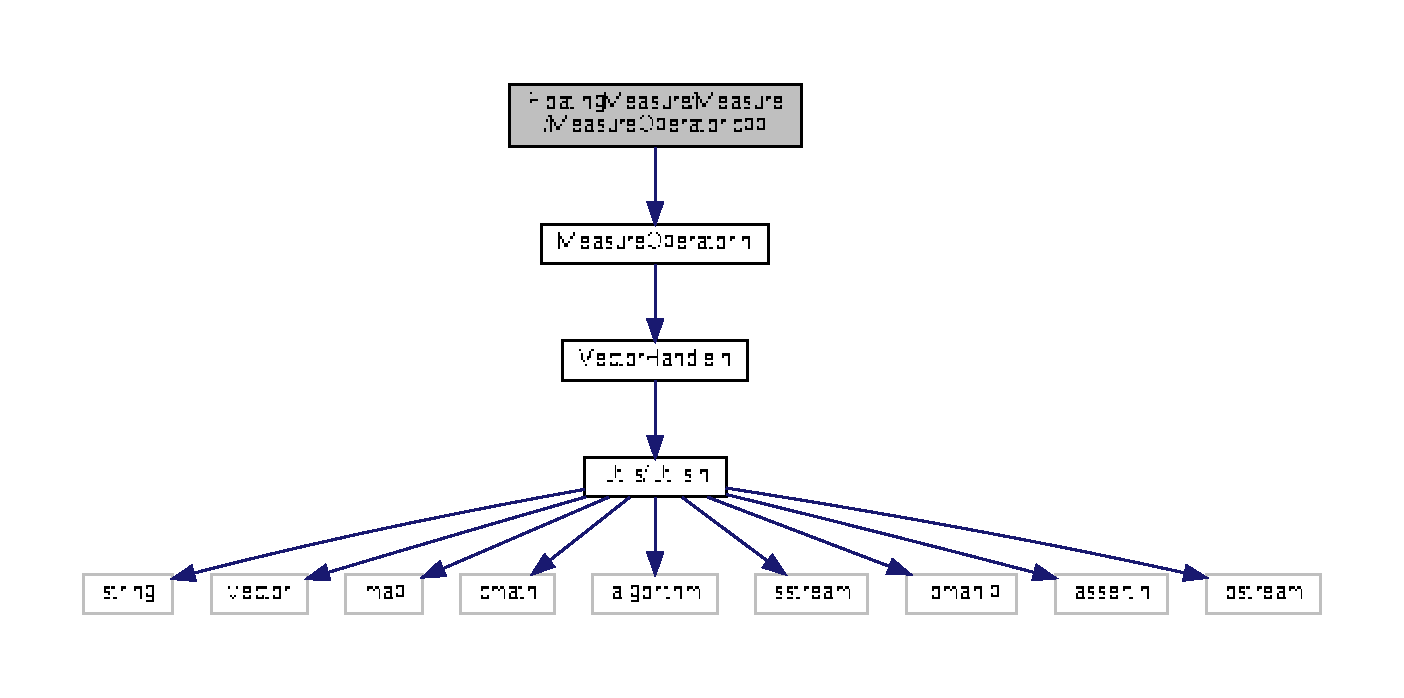
\includegraphics[width=350pt]{d0/d31/MeasureOperator_8cpp__incl}
\end{center}
\end{figure}
\subsection*{Functions}
\begin{DoxyCompactItemize}
\item 
void \hyperlink{MeasureOperator_8cpp_a86148dc43697b9309117862f69901315}{Invert} (\hyperlink{MeasureOperator_8h_a1431c79e3ad4b4c5bcc9f31f188538f2}{e\+Operation} \&Op2\+Invert)
\begin{DoxyCompactList}\small\item\em inverts given operation (e.\+g. \char`\"{}$\ast$\char`\"{} --$>$ \char`\"{}/\char`\"{}) \end{DoxyCompactList}\end{DoxyCompactItemize}


\subsection{Function Documentation}
\mbox{\Hypertarget{MeasureOperator_8cpp_a86148dc43697b9309117862f69901315}\label{MeasureOperator_8cpp_a86148dc43697b9309117862f69901315}} 
\index{Measure\+Operator.\+cpp@{Measure\+Operator.\+cpp}!Invert@{Invert}}
\index{Invert@{Invert}!Measure\+Operator.\+cpp@{Measure\+Operator.\+cpp}}
\subsubsection{\texorpdfstring{Invert()}{Invert()}}
{\footnotesize\ttfamily void Invert (\begin{DoxyParamCaption}\item[{\hyperlink{MeasureOperator_8h_a1431c79e3ad4b4c5bcc9f31f188538f2}{e\+Operation} \&}]{Op2\+Invert }\end{DoxyParamCaption})}



inverts given operation (e.\+g. \char`\"{}$\ast$\char`\"{} --$>$ \char`\"{}/\char`\"{}) 


\begin{DoxyParams}{Parameters}
{\em Op2\+Invert} & e\+Operation to invert \\
\hline
\end{DoxyParams}


Definition at line 52 of file Measure\+Operator.\+cpp.



References op\+Divide, and op\+Mult.


\hypertarget{MeasureOperator_8h}{}\section{Floating\+Measure/\+Measure/\+Measure\+Operator.h File Reference}
\label{MeasureOperator_8h}\index{Floating\+Measure/\+Measure/\+Measure\+Operator.\+h@{Floating\+Measure/\+Measure/\+Measure\+Operator.\+h}}
{\ttfamily \#include \char`\"{}Vector\+Handle.\+h\char`\"{}}\newline
Include dependency graph for Measure\+Operator.\+h\+:\nopagebreak
\begin{figure}[H]
\begin{center}
\leavevmode
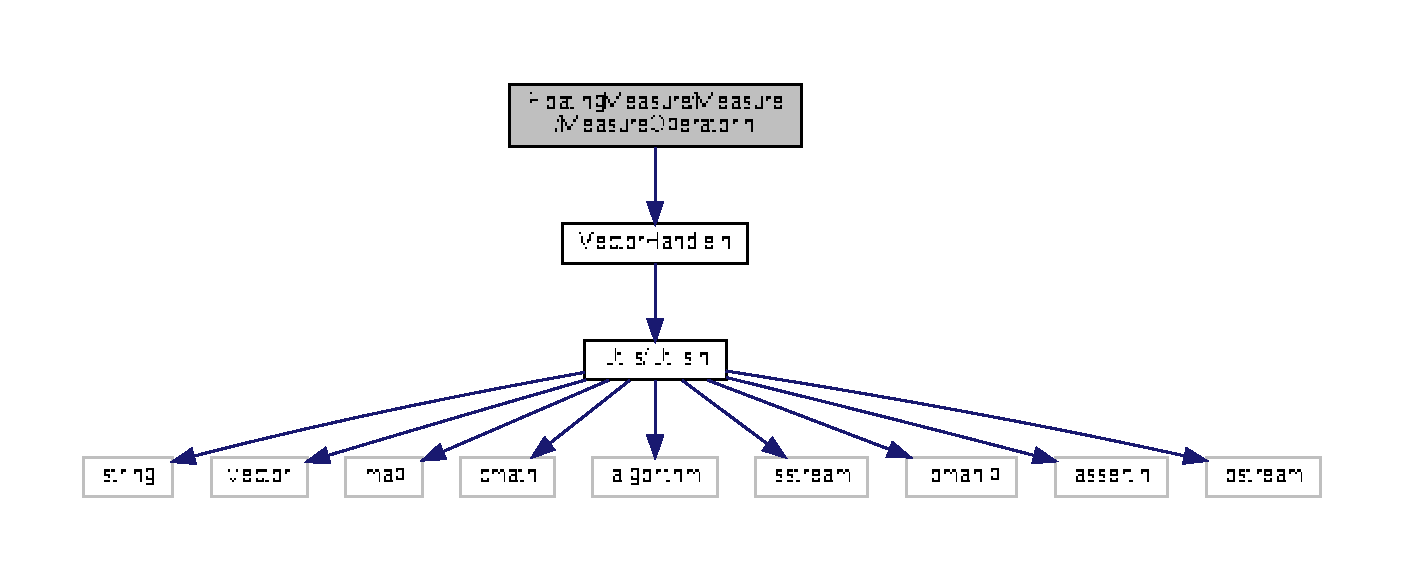
\includegraphics[width=350pt]{d6/d81/MeasureOperator_8h__incl}
\end{center}
\end{figure}
This graph shows which files directly or indirectly include this file\+:\nopagebreak
\begin{figure}[H]
\begin{center}
\leavevmode
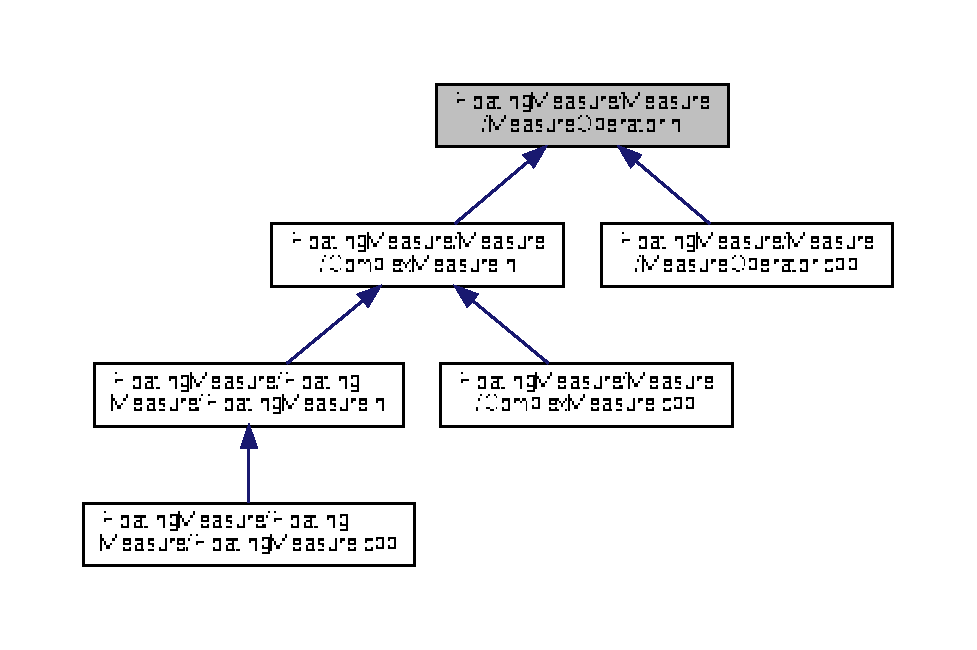
\includegraphics[width=350pt]{d1/dd6/MeasureOperator_8h__dep__incl}
\end{center}
\end{figure}
\subsection*{Classes}
\begin{DoxyCompactItemize}
\item 
class \hyperlink{classCMeasureOperator}{C\+Measure\+Operator}
\begin{DoxyCompactList}\small\item\em \hyperlink{classCMeasureOperator}{C\+Measure\+Operator}\+: this class is actually unused ... \end{DoxyCompactList}\end{DoxyCompactItemize}
\subsection*{Typedefs}
\begin{DoxyCompactItemize}
\item 
typedef \hyperlink{classCSingleton}{C\+Singleton}$<$ \hyperlink{classCMeasureOperator}{C\+Measure\+Operator} $>$ \hyperlink{MeasureOperator_8h_a1a0e805bf5f6abc66c539334ba61b71d}{C\+Measure\+Operator\+Singleton}
\end{DoxyCompactItemize}
\subsection*{Enumerations}
\begin{DoxyCompactItemize}
\item 
enum \hyperlink{MeasureOperator_8h_a1431c79e3ad4b4c5bcc9f31f188538f2}{e\+Operation} \{ \hyperlink{MeasureOperator_8h_a1431c79e3ad4b4c5bcc9f31f188538f2ad474827f099ae98a2f2c92e1ef548eb2}{op\+Mult} = 0, 
\hyperlink{MeasureOperator_8h_a1431c79e3ad4b4c5bcc9f31f188538f2a160251a34f9a9a8ee362dc477d5ba790}{op\+Divide}, 
\hyperlink{MeasureOperator_8h_a1431c79e3ad4b4c5bcc9f31f188538f2a4ac5cfcc81d8ef3e62f3225e0fd628c0}{op\+Last}, 
\hyperlink{MeasureOperator_8h_a1431c79e3ad4b4c5bcc9f31f188538f2a1ad0abc0f188cec5dffb84b17813ad6e}{op\+Unknown} = op\+Last
 \}
\end{DoxyCompactItemize}
\subsection*{Functions}
\begin{DoxyCompactItemize}
\item 
void \hyperlink{MeasureOperator_8h_a86148dc43697b9309117862f69901315}{Invert} (\hyperlink{MeasureOperator_8h_a1431c79e3ad4b4c5bcc9f31f188538f2}{e\+Operation} \&Op2\+Invert)
\begin{DoxyCompactList}\small\item\em inverts given operation (e.\+g. \char`\"{}$\ast$\char`\"{} --$>$ \char`\"{}/\char`\"{}) \end{DoxyCompactList}\end{DoxyCompactItemize}


\subsection{Typedef Documentation}
\mbox{\Hypertarget{MeasureOperator_8h_a1a0e805bf5f6abc66c539334ba61b71d}\label{MeasureOperator_8h_a1a0e805bf5f6abc66c539334ba61b71d}} 
\index{Measure\+Operator.\+h@{Measure\+Operator.\+h}!C\+Measure\+Operator\+Singleton@{C\+Measure\+Operator\+Singleton}}
\index{C\+Measure\+Operator\+Singleton@{C\+Measure\+Operator\+Singleton}!Measure\+Operator.\+h@{Measure\+Operator.\+h}}
\subsubsection{\texorpdfstring{C\+Measure\+Operator\+Singleton}{CMeasureOperatorSingleton}}
{\footnotesize\ttfamily typedef \hyperlink{classCSingleton}{C\+Singleton}$<$\hyperlink{classCMeasureOperator}{C\+Measure\+Operator}$>$ \hyperlink{MeasureOperator_8h_a1a0e805bf5f6abc66c539334ba61b71d}{C\+Measure\+Operator\+Singleton}}



Definition at line 69 of file Measure\+Operator.\+h.



\subsection{Enumeration Type Documentation}
\mbox{\Hypertarget{MeasureOperator_8h_a1431c79e3ad4b4c5bcc9f31f188538f2}\label{MeasureOperator_8h_a1431c79e3ad4b4c5bcc9f31f188538f2}} 
\index{Measure\+Operator.\+h@{Measure\+Operator.\+h}!e\+Operation@{e\+Operation}}
\index{e\+Operation@{e\+Operation}!Measure\+Operator.\+h@{Measure\+Operator.\+h}}
\subsubsection{\texorpdfstring{e\+Operation}{eOperation}}
{\footnotesize\ttfamily enum \hyperlink{MeasureOperator_8h_a1431c79e3ad4b4c5bcc9f31f188538f2}{e\+Operation}}

\begin{DoxyEnumFields}{Enumerator}
\raisebox{\heightof{T}}[0pt][0pt]{\index{op\+Mult@{op\+Mult}!Measure\+Operator.\+h@{Measure\+Operator.\+h}}\index{Measure\+Operator.\+h@{Measure\+Operator.\+h}!op\+Mult@{op\+Mult}}}\mbox{\Hypertarget{MeasureOperator_8h_a1431c79e3ad4b4c5bcc9f31f188538f2ad474827f099ae98a2f2c92e1ef548eb2}\label{MeasureOperator_8h_a1431c79e3ad4b4c5bcc9f31f188538f2ad474827f099ae98a2f2c92e1ef548eb2}} 
op\+Mult&0 \+: multiplication is the starting element \\
\hline

\raisebox{\heightof{T}}[0pt][0pt]{\index{op\+Divide@{op\+Divide}!Measure\+Operator.\+h@{Measure\+Operator.\+h}}\index{Measure\+Operator.\+h@{Measure\+Operator.\+h}!op\+Divide@{op\+Divide}}}\mbox{\Hypertarget{MeasureOperator_8h_a1431c79e3ad4b4c5bcc9f31f188538f2a160251a34f9a9a8ee362dc477d5ba790}\label{MeasureOperator_8h_a1431c79e3ad4b4c5bcc9f31f188538f2a160251a34f9a9a8ee362dc477d5ba790}} 
op\+Divide&1 \+: division \\
\hline

\raisebox{\heightof{T}}[0pt][0pt]{\index{op\+Last@{op\+Last}!Measure\+Operator.\+h@{Measure\+Operator.\+h}}\index{Measure\+Operator.\+h@{Measure\+Operator.\+h}!op\+Last@{op\+Last}}}\mbox{\Hypertarget{MeasureOperator_8h_a1431c79e3ad4b4c5bcc9f31f188538f2a4ac5cfcc81d8ef3e62f3225e0fd628c0}\label{MeasureOperator_8h_a1431c79e3ad4b4c5bcc9f31f188538f2a4ac5cfcc81d8ef3e62f3225e0fd628c0}} 
op\+Last&2 \+: last operation ... invalid (for iteration) \\
\hline

\raisebox{\heightof{T}}[0pt][0pt]{\index{op\+Unknown@{op\+Unknown}!Measure\+Operator.\+h@{Measure\+Operator.\+h}}\index{Measure\+Operator.\+h@{Measure\+Operator.\+h}!op\+Unknown@{op\+Unknown}}}\mbox{\Hypertarget{MeasureOperator_8h_a1431c79e3ad4b4c5bcc9f31f188538f2a1ad0abc0f188cec5dffb84b17813ad6e}\label{MeasureOperator_8h_a1431c79e3ad4b4c5bcc9f31f188538f2a1ad0abc0f188cec5dffb84b17813ad6e}} 
op\+Unknown&3 \+: invalid operation = last operation \\
\hline

\end{DoxyEnumFields}


Definition at line 30 of file Measure\+Operator.\+h.



\subsection{Function Documentation}
\mbox{\Hypertarget{MeasureOperator_8h_a86148dc43697b9309117862f69901315}\label{MeasureOperator_8h_a86148dc43697b9309117862f69901315}} 
\index{Measure\+Operator.\+h@{Measure\+Operator.\+h}!Invert@{Invert}}
\index{Invert@{Invert}!Measure\+Operator.\+h@{Measure\+Operator.\+h}}
\subsubsection{\texorpdfstring{Invert()}{Invert()}}
{\footnotesize\ttfamily void Invert (\begin{DoxyParamCaption}\item[{\hyperlink{MeasureOperator_8h_a1431c79e3ad4b4c5bcc9f31f188538f2}{e\+Operation} \&}]{Op2\+Invert }\end{DoxyParamCaption})}



inverts given operation (e.\+g. \char`\"{}$\ast$\char`\"{} --$>$ \char`\"{}/\char`\"{}) 


\begin{DoxyParams}{Parameters}
{\em Op2\+Invert} & e\+Operation to invert \\
\hline
\end{DoxyParams}


Definition at line 52 of file Measure\+Operator.\+cpp.



References op\+Divide, and op\+Mult.


\hypertarget{PreMeasure_8cpp}{}\section{Floating\+Measure/\+Measure/\+Pre\+Measure.cpp File Reference}
\label{PreMeasure_8cpp}\index{Floating\+Measure/\+Measure/\+Pre\+Measure.\+cpp@{Floating\+Measure/\+Measure/\+Pre\+Measure.\+cpp}}
{\ttfamily \#include \char`\"{}Measure/\+Pre\+Measure.\+h\char`\"{}}\newline
Include dependency graph for Pre\+Measure.\+cpp\+:\nopagebreak
\begin{figure}[H]
\begin{center}
\leavevmode
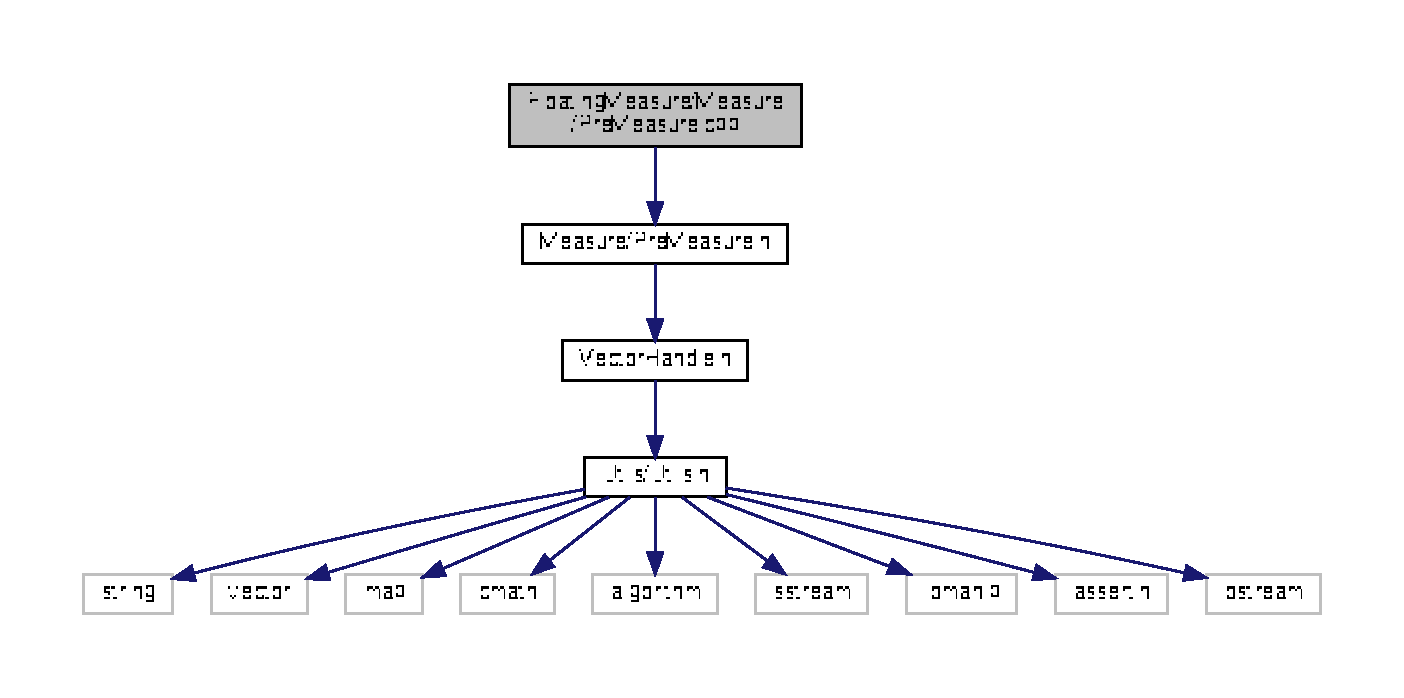
\includegraphics[width=350pt]{d5/d20/PreMeasure_8cpp__incl}
\end{center}
\end{figure}

\hypertarget{PreMeasure_8h}{}\section{Floating\+Measure/\+Measure/\+Pre\+Measure.h File Reference}
\label{PreMeasure_8h}\index{Floating\+Measure/\+Measure/\+Pre\+Measure.\+h@{Floating\+Measure/\+Measure/\+Pre\+Measure.\+h}}
{\ttfamily \#include \char`\"{}Vector\+Handle.\+h\char`\"{}}\newline
Include dependency graph for Pre\+Measure.\+h\+:\nopagebreak
\begin{figure}[H]
\begin{center}
\leavevmode
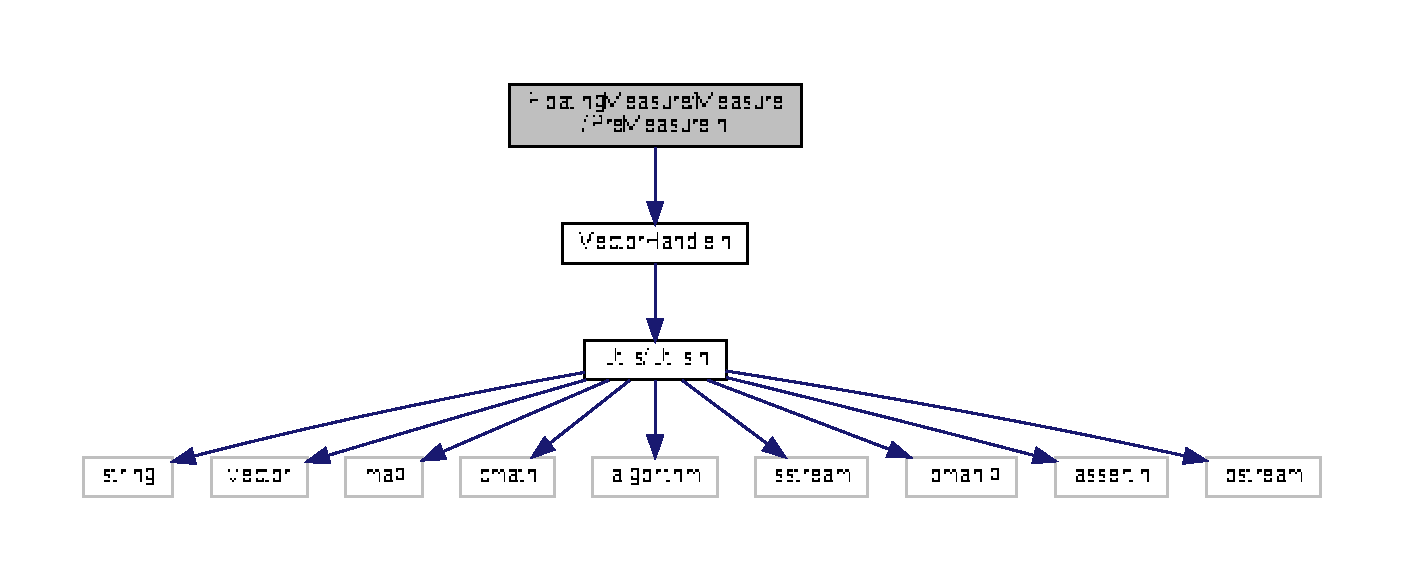
\includegraphics[width=350pt]{d7/d67/PreMeasure_8h__incl}
\end{center}
\end{figure}
This graph shows which files directly or indirectly include this file\+:\nopagebreak
\begin{figure}[H]
\begin{center}
\leavevmode
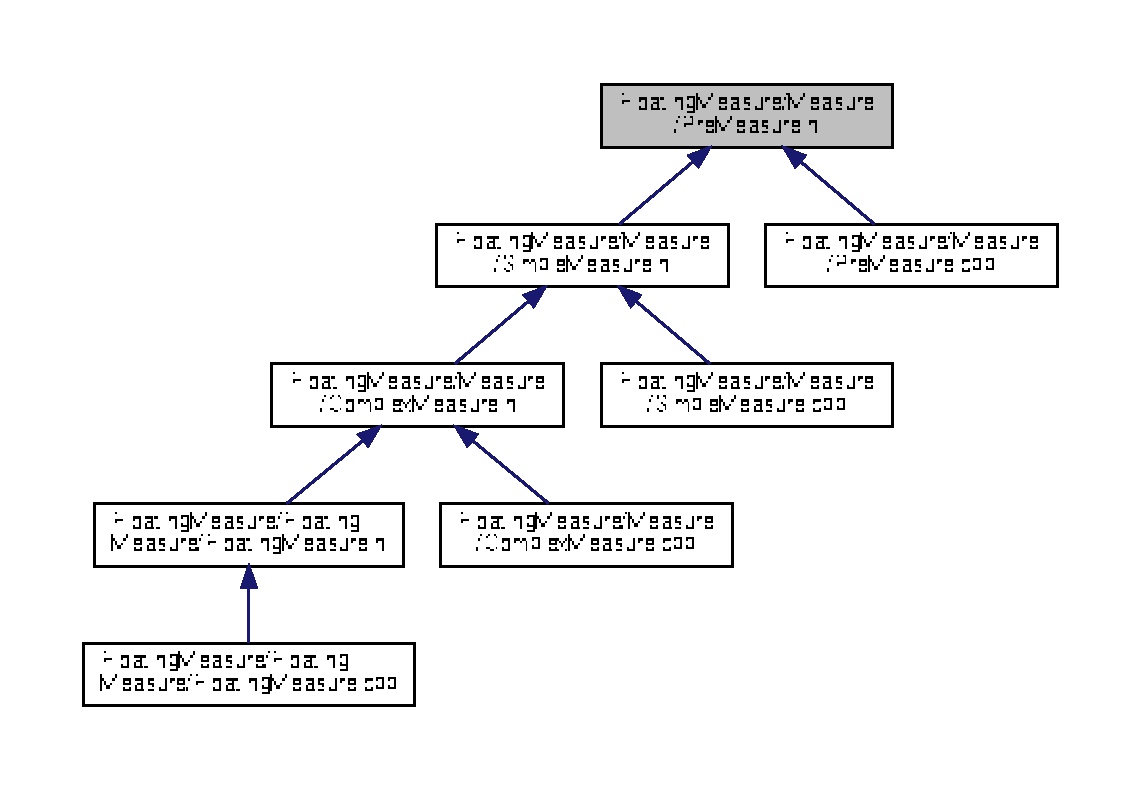
\includegraphics[width=350pt]{dd/d40/PreMeasure_8h__dep__incl}
\end{center}
\end{figure}
\subsection*{Classes}
\begin{DoxyCompactItemize}
\item 
class \hyperlink{classCPreMeasure}{C\+Pre\+Measure}
\begin{DoxyCompactList}\small\item\em \hyperlink{classCPreMeasure}{C\+Pre\+Measure} represents the pre-\/measure part of a measure. ~\newline
 For example milli volt consists of the base-\/measure part \char`\"{}\+Volt\char`\"{} (see \hyperlink{classCBaseMeasure}{C\+Base\+Measure}) and the pre-\/measure part \char`\"{}milli\char`\"{}. ~\newline
 This class handles vectors of\+: \end{DoxyCompactList}\end{DoxyCompactItemize}
\subsection*{Macros}
\begin{DoxyCompactItemize}
\item 
\#define \hyperlink{PreMeasure_8h_a349316092037fdd0773335fab4e15ee8}{P\+RE}~\hyperlink{classCSingleton_a58f5ac3aaaea8079a373350594726bdf}{C\+Pre\+Measure\+Singleton\+::instance}()
\begin{DoxyCompactList}\small\item\em Short cut to the singleton instance of \hyperlink{classCPreMeasure}{C\+Pre\+Measure}. \end{DoxyCompactList}\end{DoxyCompactItemize}
\subsection*{Typedefs}
\begin{DoxyCompactItemize}
\item 
typedef \hyperlink{classCSingleton}{C\+Singleton}$<$ \hyperlink{classCPreMeasure}{C\+Pre\+Measure} $>$ \hyperlink{PreMeasure_8h_af3953554ad21c10a9769a189bc1352af}{C\+Pre\+Measure\+Singleton}
\begin{DoxyCompactList}\small\item\em a singleton instance of the class \hyperlink{classCPreMeasure}{C\+Pre\+Measure}\+: use this for efficient memory handling \end{DoxyCompactList}\end{DoxyCompactItemize}
\subsection*{Enumerations}
\begin{DoxyCompactItemize}
\item 
enum \hyperlink{PreMeasure_8h_a6c81167b8d4c2badde42f81cb7214620}{e\+Pre\+Measure} \{ \newline
\hyperlink{PreMeasure_8h_a6c81167b8d4c2badde42f81cb7214620afaa8a9cf6a5dc121c52ccd6f50c3ffed}{pm\+Femto} = 0, 
\hyperlink{PreMeasure_8h_a6c81167b8d4c2badde42f81cb7214620a9a2f91f1e3f54c88046c10dcbfa08a3d}{pm\+First} = pm\+Femto, 
\hyperlink{PreMeasure_8h_a6c81167b8d4c2badde42f81cb7214620a98d02efe76075e56d8ec6ecce1fd7e67}{pm\+Piko}, 
\hyperlink{PreMeasure_8h_a6c81167b8d4c2badde42f81cb7214620a97a6d10912fda5efedb5209ff94e11b2}{pm\+Nano}, 
\newline
\hyperlink{PreMeasure_8h_a6c81167b8d4c2badde42f81cb7214620a186f37857e13cbb45bcbbb97c2c15561}{pm\+Micro}, 
\hyperlink{PreMeasure_8h_a6c81167b8d4c2badde42f81cb7214620aff93812e5c2f401cb10fe430a1d341f4}{pm\+Milli}, 
\hyperlink{PreMeasure_8h_a6c81167b8d4c2badde42f81cb7214620af7eea43f9cd732ef8e43005aeb46f0f3}{pm\+Centi}, 
\hyperlink{PreMeasure_8h_a6c81167b8d4c2badde42f81cb7214620a1266f4c6263ccd31d9f853fb3993e7b2}{pm\+Deci}, 
\newline
\hyperlink{PreMeasure_8h_a6c81167b8d4c2badde42f81cb7214620a32bf0cb12587b174b949f8568c9ec0c3}{pm\+Ident}, 
\hyperlink{PreMeasure_8h_a6c81167b8d4c2badde42f81cb7214620a11d938995c9d37cb2b34f454cb5b3f2c}{pm\+Deca}, 
\hyperlink{PreMeasure_8h_a6c81167b8d4c2badde42f81cb7214620ade3242e2b12643a93f3849785691d86c}{pm\+Hecto}, 
\hyperlink{PreMeasure_8h_a6c81167b8d4c2badde42f81cb7214620acdf63dcd9d24a1d774d2fe923621ca69}{pm\+Kilo}, 
\newline
\hyperlink{PreMeasure_8h_a6c81167b8d4c2badde42f81cb7214620ac669ac8a067bd6491c426c00af19f085}{pm\+Mega}, 
\hyperlink{PreMeasure_8h_a6c81167b8d4c2badde42f81cb7214620a0d6643b3b85f89178a09db0897ef502c}{pm\+Giga}, 
\hyperlink{PreMeasure_8h_a6c81167b8d4c2badde42f81cb7214620a70676cd51c6e17853f7cad277f473afd}{pm\+Tera}, 
\hyperlink{PreMeasure_8h_a6c81167b8d4c2badde42f81cb7214620add0b3a1d027f070cedc49b5193daebba}{pm\+Peta}, 
\newline
\hyperlink{PreMeasure_8h_a6c81167b8d4c2badde42f81cb7214620abe0b5d6c4697d04c36b1425a519fc128}{pm\+Exa}, 
\hyperlink{PreMeasure_8h_a6c81167b8d4c2badde42f81cb7214620a00b29f37d368d66abc95fee7ecf9a034}{pm\+Zetta}, 
\hyperlink{PreMeasure_8h_a6c81167b8d4c2badde42f81cb7214620a5481dc587dbf4b25ddec4d4aed8e2ccb}{pm\+Yotta}, 
\hyperlink{PreMeasure_8h_a6c81167b8d4c2badde42f81cb7214620ad74e7f79c20123c3ef2128f62deb6857}{pm\+Last}, 
\newline
\hyperlink{PreMeasure_8h_a6c81167b8d4c2badde42f81cb7214620a45907e80ae387e2b4a105be6f3276313}{pm\+Unknown} = pm\+Last
 \}\begin{DoxyCompactList}\small\item\em enum for indexing the vectors of \hyperlink{classCPreMeasure}{C\+Pre\+Measure} \end{DoxyCompactList}
\end{DoxyCompactItemize}


\subsection{Macro Definition Documentation}
\mbox{\Hypertarget{PreMeasure_8h_a349316092037fdd0773335fab4e15ee8}\label{PreMeasure_8h_a349316092037fdd0773335fab4e15ee8}} 
\index{Pre\+Measure.\+h@{Pre\+Measure.\+h}!P\+RE@{P\+RE}}
\index{P\+RE@{P\+RE}!Pre\+Measure.\+h@{Pre\+Measure.\+h}}
\subsubsection{\texorpdfstring{P\+RE}{PRE}}
{\footnotesize\ttfamily \#define P\+RE~\hyperlink{classCSingleton_a58f5ac3aaaea8079a373350594726bdf}{C\+Pre\+Measure\+Singleton\+::instance}()}



Short cut to the singleton instance of \hyperlink{classCPreMeasure}{C\+Pre\+Measure}. 



Definition at line 198 of file Pre\+Measure.\+h.



\subsection{Typedef Documentation}
\mbox{\Hypertarget{PreMeasure_8h_af3953554ad21c10a9769a189bc1352af}\label{PreMeasure_8h_af3953554ad21c10a9769a189bc1352af}} 
\index{Pre\+Measure.\+h@{Pre\+Measure.\+h}!C\+Pre\+Measure\+Singleton@{C\+Pre\+Measure\+Singleton}}
\index{C\+Pre\+Measure\+Singleton@{C\+Pre\+Measure\+Singleton}!Pre\+Measure.\+h@{Pre\+Measure.\+h}}
\subsubsection{\texorpdfstring{C\+Pre\+Measure\+Singleton}{CPreMeasureSingleton}}
{\footnotesize\ttfamily typedef \hyperlink{classCSingleton}{C\+Singleton}$<$\hyperlink{classCPreMeasure}{C\+Pre\+Measure}$>$ \hyperlink{PreMeasure_8h_af3953554ad21c10a9769a189bc1352af}{C\+Pre\+Measure\+Singleton}}



a singleton instance of the class \hyperlink{classCPreMeasure}{C\+Pre\+Measure}\+: use this for efficient memory handling 



Definition at line 191 of file Pre\+Measure.\+h.



\subsection{Enumeration Type Documentation}
\mbox{\Hypertarget{PreMeasure_8h_a6c81167b8d4c2badde42f81cb7214620}\label{PreMeasure_8h_a6c81167b8d4c2badde42f81cb7214620}} 
\index{Pre\+Measure.\+h@{Pre\+Measure.\+h}!e\+Pre\+Measure@{e\+Pre\+Measure}}
\index{e\+Pre\+Measure@{e\+Pre\+Measure}!Pre\+Measure.\+h@{Pre\+Measure.\+h}}
\subsubsection{\texorpdfstring{e\+Pre\+Measure}{ePreMeasure}}
{\footnotesize\ttfamily enum \hyperlink{PreMeasure_8h_a6c81167b8d4c2badde42f81cb7214620}{e\+Pre\+Measure}}



enum for indexing the vectors of \hyperlink{classCPreMeasure}{C\+Pre\+Measure} 

\begin{DoxyEnumFields}{Enumerator}
\raisebox{\heightof{T}}[0pt][0pt]{\index{pm\+Femto@{pm\+Femto}!Pre\+Measure.\+h@{Pre\+Measure.\+h}}\index{Pre\+Measure.\+h@{Pre\+Measure.\+h}!pm\+Femto@{pm\+Femto}}}\mbox{\Hypertarget{PreMeasure_8h_a6c81167b8d4c2badde42f81cb7214620afaa8a9cf6a5dc121c52ccd6f50c3ffed}\label{PreMeasure_8h_a6c81167b8d4c2badde42f81cb7214620afaa8a9cf6a5dc121c52ccd6f50c3ffed}} 
pm\+Femto&0 factor = 10 \textsuperscript{ ⁻15 }, exp10\+: -\/15, short\+: \char`\"{}f\char`\"{}, long\+: \char`\"{}femto\char`\"{} \\
\hline

\raisebox{\heightof{T}}[0pt][0pt]{\index{pm\+First@{pm\+First}!Pre\+Measure.\+h@{Pre\+Measure.\+h}}\index{Pre\+Measure.\+h@{Pre\+Measure.\+h}!pm\+First@{pm\+First}}}\mbox{\Hypertarget{PreMeasure_8h_a6c81167b8d4c2badde42f81cb7214620a9a2f91f1e3f54c88046c10dcbfa08a3d}\label{PreMeasure_8h_a6c81167b8d4c2badde42f81cb7214620a9a2f91f1e3f54c88046c10dcbfa08a3d}} 
pm\+First&0 starting index \char`\"{}femto\char`\"{} \\
\hline

\raisebox{\heightof{T}}[0pt][0pt]{\index{pm\+Piko@{pm\+Piko}!Pre\+Measure.\+h@{Pre\+Measure.\+h}}\index{Pre\+Measure.\+h@{Pre\+Measure.\+h}!pm\+Piko@{pm\+Piko}}}\mbox{\Hypertarget{PreMeasure_8h_a6c81167b8d4c2badde42f81cb7214620a98d02efe76075e56d8ec6ecce1fd7e67}\label{PreMeasure_8h_a6c81167b8d4c2badde42f81cb7214620a98d02efe76075e56d8ec6ecce1fd7e67}} 
pm\+Piko&1 \+: factor = 10 \textsuperscript{⁻12}, exp10\+: -\/12, short\+: \char`\"{}p\char`\"{}, long\+: \char`\"{}piko\char`\"{} \\
\hline

\raisebox{\heightof{T}}[0pt][0pt]{\index{pm\+Nano@{pm\+Nano}!Pre\+Measure.\+h@{Pre\+Measure.\+h}}\index{Pre\+Measure.\+h@{Pre\+Measure.\+h}!pm\+Nano@{pm\+Nano}}}\mbox{\Hypertarget{PreMeasure_8h_a6c81167b8d4c2badde42f81cb7214620a97a6d10912fda5efedb5209ff94e11b2}\label{PreMeasure_8h_a6c81167b8d4c2badde42f81cb7214620a97a6d10912fda5efedb5209ff94e11b2}} 
pm\+Nano&2 \+: factor = 10 \textsuperscript{⁻9 }, exp10\+: -\/9, short\+: \char`\"{}n\char`\"{}, long\+: \char`\"{}nano\char`\"{} \\
\hline

\raisebox{\heightof{T}}[0pt][0pt]{\index{pm\+Micro@{pm\+Micro}!Pre\+Measure.\+h@{Pre\+Measure.\+h}}\index{Pre\+Measure.\+h@{Pre\+Measure.\+h}!pm\+Micro@{pm\+Micro}}}\mbox{\Hypertarget{PreMeasure_8h_a6c81167b8d4c2badde42f81cb7214620a186f37857e13cbb45bcbbb97c2c15561}\label{PreMeasure_8h_a6c81167b8d4c2badde42f81cb7214620a186f37857e13cbb45bcbbb97c2c15561}} 
pm\+Micro&3 \+: factor = 10 \textsuperscript{⁻6 }, exp10\+: ⁻6, short\+: "{$\mu$}", long\+: \char`\"{}micro\char`\"{} \\
\hline

\raisebox{\heightof{T}}[0pt][0pt]{\index{pm\+Milli@{pm\+Milli}!Pre\+Measure.\+h@{Pre\+Measure.\+h}}\index{Pre\+Measure.\+h@{Pre\+Measure.\+h}!pm\+Milli@{pm\+Milli}}}\mbox{\Hypertarget{PreMeasure_8h_a6c81167b8d4c2badde42f81cb7214620aff93812e5c2f401cb10fe430a1d341f4}\label{PreMeasure_8h_a6c81167b8d4c2badde42f81cb7214620aff93812e5c2f401cb10fe430a1d341f4}} 
pm\+Milli&4 \+: factor = 10 \textsuperscript{⁻3 }, exp10\+: ⁻3, short\+: \char`\"{}m\char`\"{}, long\+: \char`\"{}milli\char`\"{} \\
\hline

\raisebox{\heightof{T}}[0pt][0pt]{\index{pm\+Centi@{pm\+Centi}!Pre\+Measure.\+h@{Pre\+Measure.\+h}}\index{Pre\+Measure.\+h@{Pre\+Measure.\+h}!pm\+Centi@{pm\+Centi}}}\mbox{\Hypertarget{PreMeasure_8h_a6c81167b8d4c2badde42f81cb7214620af7eea43f9cd732ef8e43005aeb46f0f3}\label{PreMeasure_8h_a6c81167b8d4c2badde42f81cb7214620af7eea43f9cd732ef8e43005aeb46f0f3}} 
pm\+Centi&5 \+: factor = 10 \textsuperscript{⁻2 }, exp10\+: ⁻2, short\+: \char`\"{}c\char`\"{}, long\+: \char`\"{}centi\char`\"{} \\
\hline

\raisebox{\heightof{T}}[0pt][0pt]{\index{pm\+Deci@{pm\+Deci}!Pre\+Measure.\+h@{Pre\+Measure.\+h}}\index{Pre\+Measure.\+h@{Pre\+Measure.\+h}!pm\+Deci@{pm\+Deci}}}\mbox{\Hypertarget{PreMeasure_8h_a6c81167b8d4c2badde42f81cb7214620a1266f4c6263ccd31d9f853fb3993e7b2}\label{PreMeasure_8h_a6c81167b8d4c2badde42f81cb7214620a1266f4c6263ccd31d9f853fb3993e7b2}} 
pm\+Deci&6 \+: factor = 10 \textsuperscript{⁻1 }, exp10\+: ⁻1, short\+: \char`\"{}d\char`\"{}, long\+: \char`\"{}deci\char`\"{} \\
\hline

\raisebox{\heightof{T}}[0pt][0pt]{\index{pm\+Ident@{pm\+Ident}!Pre\+Measure.\+h@{Pre\+Measure.\+h}}\index{Pre\+Measure.\+h@{Pre\+Measure.\+h}!pm\+Ident@{pm\+Ident}}}\mbox{\Hypertarget{PreMeasure_8h_a6c81167b8d4c2badde42f81cb7214620a32bf0cb12587b174b949f8568c9ec0c3}\label{PreMeasure_8h_a6c81167b8d4c2badde42f81cb7214620a32bf0cb12587b174b949f8568c9ec0c3}} 
pm\+Ident&7 \+: factor = 10 \textsuperscript{ 0 }, exp10\+: 0, short\+: \char`\"{}\char`\"{}, long\+: \char`\"{}\char`\"{} \\
\hline

\raisebox{\heightof{T}}[0pt][0pt]{\index{pm\+Deca@{pm\+Deca}!Pre\+Measure.\+h@{Pre\+Measure.\+h}}\index{Pre\+Measure.\+h@{Pre\+Measure.\+h}!pm\+Deca@{pm\+Deca}}}\mbox{\Hypertarget{PreMeasure_8h_a6c81167b8d4c2badde42f81cb7214620a11d938995c9d37cb2b34f454cb5b3f2c}\label{PreMeasure_8h_a6c81167b8d4c2badde42f81cb7214620a11d938995c9d37cb2b34f454cb5b3f2c}} 
pm\+Deca&8 \+: factor = 10 \textsuperscript{+1 }, exp10\+: +1, short\+: \char`\"{}da\char`\"{}, long\+: \char`\"{}deca\char`\"{} \\
\hline

\raisebox{\heightof{T}}[0pt][0pt]{\index{pm\+Hecto@{pm\+Hecto}!Pre\+Measure.\+h@{Pre\+Measure.\+h}}\index{Pre\+Measure.\+h@{Pre\+Measure.\+h}!pm\+Hecto@{pm\+Hecto}}}\mbox{\Hypertarget{PreMeasure_8h_a6c81167b8d4c2badde42f81cb7214620ade3242e2b12643a93f3849785691d86c}\label{PreMeasure_8h_a6c81167b8d4c2badde42f81cb7214620ade3242e2b12643a93f3849785691d86c}} 
pm\+Hecto&9 \+: factor = 10 \textsuperscript{+2 }, exp10\+: +2, short\+: \char`\"{}h\char`\"{}, long\+: \char`\"{}hecto\char`\"{} \\
\hline

\raisebox{\heightof{T}}[0pt][0pt]{\index{pm\+Kilo@{pm\+Kilo}!Pre\+Measure.\+h@{Pre\+Measure.\+h}}\index{Pre\+Measure.\+h@{Pre\+Measure.\+h}!pm\+Kilo@{pm\+Kilo}}}\mbox{\Hypertarget{PreMeasure_8h_a6c81167b8d4c2badde42f81cb7214620acdf63dcd9d24a1d774d2fe923621ca69}\label{PreMeasure_8h_a6c81167b8d4c2badde42f81cb7214620acdf63dcd9d24a1d774d2fe923621ca69}} 
pm\+Kilo&10 \+: factor = 10 \textsuperscript{+3 }, exp10\+: +3, short\+: \char`\"{}k\char`\"{}, long\+: \char`\"{}kilo\char`\"{} \\
\hline

\raisebox{\heightof{T}}[0pt][0pt]{\index{pm\+Mega@{pm\+Mega}!Pre\+Measure.\+h@{Pre\+Measure.\+h}}\index{Pre\+Measure.\+h@{Pre\+Measure.\+h}!pm\+Mega@{pm\+Mega}}}\mbox{\Hypertarget{PreMeasure_8h_a6c81167b8d4c2badde42f81cb7214620ac669ac8a067bd6491c426c00af19f085}\label{PreMeasure_8h_a6c81167b8d4c2badde42f81cb7214620ac669ac8a067bd6491c426c00af19f085}} 
pm\+Mega&11 \+: factor = 10 \textsuperscript{+6 }, exp10\+: +6, short\+: \char`\"{}\+M\char`\"{}, long\+: \char`\"{}mega\char`\"{} \\
\hline

\raisebox{\heightof{T}}[0pt][0pt]{\index{pm\+Giga@{pm\+Giga}!Pre\+Measure.\+h@{Pre\+Measure.\+h}}\index{Pre\+Measure.\+h@{Pre\+Measure.\+h}!pm\+Giga@{pm\+Giga}}}\mbox{\Hypertarget{PreMeasure_8h_a6c81167b8d4c2badde42f81cb7214620a0d6643b3b85f89178a09db0897ef502c}\label{PreMeasure_8h_a6c81167b8d4c2badde42f81cb7214620a0d6643b3b85f89178a09db0897ef502c}} 
pm\+Giga&12 \+: factor = 10 \textsuperscript{+9 }, exp10\+: +9, short\+: \char`\"{}\+G\char`\"{}, long\+: \char`\"{}giga\char`\"{} \\
\hline

\raisebox{\heightof{T}}[0pt][0pt]{\index{pm\+Tera@{pm\+Tera}!Pre\+Measure.\+h@{Pre\+Measure.\+h}}\index{Pre\+Measure.\+h@{Pre\+Measure.\+h}!pm\+Tera@{pm\+Tera}}}\mbox{\Hypertarget{PreMeasure_8h_a6c81167b8d4c2badde42f81cb7214620a70676cd51c6e17853f7cad277f473afd}\label{PreMeasure_8h_a6c81167b8d4c2badde42f81cb7214620a70676cd51c6e17853f7cad277f473afd}} 
pm\+Tera&13 \+: factor = 10 \textsuperscript{+12}, exp10\+: +12, short\+: \char`\"{}\+T\char`\"{}, long\+: \char`\"{}tera\char`\"{} \\
\hline

\raisebox{\heightof{T}}[0pt][0pt]{\index{pm\+Peta@{pm\+Peta}!Pre\+Measure.\+h@{Pre\+Measure.\+h}}\index{Pre\+Measure.\+h@{Pre\+Measure.\+h}!pm\+Peta@{pm\+Peta}}}\mbox{\Hypertarget{PreMeasure_8h_a6c81167b8d4c2badde42f81cb7214620add0b3a1d027f070cedc49b5193daebba}\label{PreMeasure_8h_a6c81167b8d4c2badde42f81cb7214620add0b3a1d027f070cedc49b5193daebba}} 
pm\+Peta&14 \+: factor = 10 \textsuperscript{+15}, exp10\+: +15, short\+: \char`\"{}\+P\char`\"{}, long\+: \char`\"{}peta\char`\"{} \\
\hline

\raisebox{\heightof{T}}[0pt][0pt]{\index{pm\+Exa@{pm\+Exa}!Pre\+Measure.\+h@{Pre\+Measure.\+h}}\index{Pre\+Measure.\+h@{Pre\+Measure.\+h}!pm\+Exa@{pm\+Exa}}}\mbox{\Hypertarget{PreMeasure_8h_a6c81167b8d4c2badde42f81cb7214620abe0b5d6c4697d04c36b1425a519fc128}\label{PreMeasure_8h_a6c81167b8d4c2badde42f81cb7214620abe0b5d6c4697d04c36b1425a519fc128}} 
pm\+Exa&15 \+: factor = 10 \textsuperscript{+18}, exp10\+: +18, short\+: \char`\"{}\+E\char`\"{}, long\+: \char`\"{}exa\char`\"{} \\
\hline

\raisebox{\heightof{T}}[0pt][0pt]{\index{pm\+Zetta@{pm\+Zetta}!Pre\+Measure.\+h@{Pre\+Measure.\+h}}\index{Pre\+Measure.\+h@{Pre\+Measure.\+h}!pm\+Zetta@{pm\+Zetta}}}\mbox{\Hypertarget{PreMeasure_8h_a6c81167b8d4c2badde42f81cb7214620a00b29f37d368d66abc95fee7ecf9a034}\label{PreMeasure_8h_a6c81167b8d4c2badde42f81cb7214620a00b29f37d368d66abc95fee7ecf9a034}} 
pm\+Zetta&16 \+: factor = 10 \textsuperscript{+21}, exp10\+: +21, short\+: \char`\"{}\+Z\char`\"{}, long\+: \char`\"{}zetta\char`\"{} \\
\hline

\raisebox{\heightof{T}}[0pt][0pt]{\index{pm\+Yotta@{pm\+Yotta}!Pre\+Measure.\+h@{Pre\+Measure.\+h}}\index{Pre\+Measure.\+h@{Pre\+Measure.\+h}!pm\+Yotta@{pm\+Yotta}}}\mbox{\Hypertarget{PreMeasure_8h_a6c81167b8d4c2badde42f81cb7214620a5481dc587dbf4b25ddec4d4aed8e2ccb}\label{PreMeasure_8h_a6c81167b8d4c2badde42f81cb7214620a5481dc587dbf4b25ddec4d4aed8e2ccb}} 
pm\+Yotta&17 \+: factor = 10 \textsuperscript{+24}, exp10\+: +24, short\+: \char`\"{}\+Y\char`\"{}, long\+: \char`\"{}yotta\char`\"{} \\
\hline

\raisebox{\heightof{T}}[0pt][0pt]{\index{pm\+Last@{pm\+Last}!Pre\+Measure.\+h@{Pre\+Measure.\+h}}\index{Pre\+Measure.\+h@{Pre\+Measure.\+h}!pm\+Last@{pm\+Last}}}\mbox{\Hypertarget{PreMeasure_8h_a6c81167b8d4c2badde42f81cb7214620ad74e7f79c20123c3ef2128f62deb6857}\label{PreMeasure_8h_a6c81167b8d4c2badde42f81cb7214620ad74e7f79c20123c3ef2128f62deb6857}} 
pm\+Last&18 \+: invalid last index \\
\hline

\raisebox{\heightof{T}}[0pt][0pt]{\index{pm\+Unknown@{pm\+Unknown}!Pre\+Measure.\+h@{Pre\+Measure.\+h}}\index{Pre\+Measure.\+h@{Pre\+Measure.\+h}!pm\+Unknown@{pm\+Unknown}}}\mbox{\Hypertarget{PreMeasure_8h_a6c81167b8d4c2badde42f81cb7214620a45907e80ae387e2b4a105be6f3276313}\label{PreMeasure_8h_a6c81167b8d4c2badde42f81cb7214620a45907e80ae387e2b4a105be6f3276313}} 
pm\+Unknown&18 \+: identical with last index \\
\hline

\end{DoxyEnumFields}


Definition at line 34 of file Pre\+Measure.\+h.


\hypertarget{SimpleMeasure_8cpp}{}\section{Floating\+Measure/\+Measure/\+Simple\+Measure.cpp File Reference}
\label{SimpleMeasure_8cpp}\index{Floating\+Measure/\+Measure/\+Simple\+Measure.\+cpp@{Floating\+Measure/\+Measure/\+Simple\+Measure.\+cpp}}
{\ttfamily \#include \char`\"{}Simple\+Measure.\+h\char`\"{}}\newline
Include dependency graph for Simple\+Measure.\+cpp\+:
\nopagebreak
\begin{figure}[H]
\begin{center}
\leavevmode
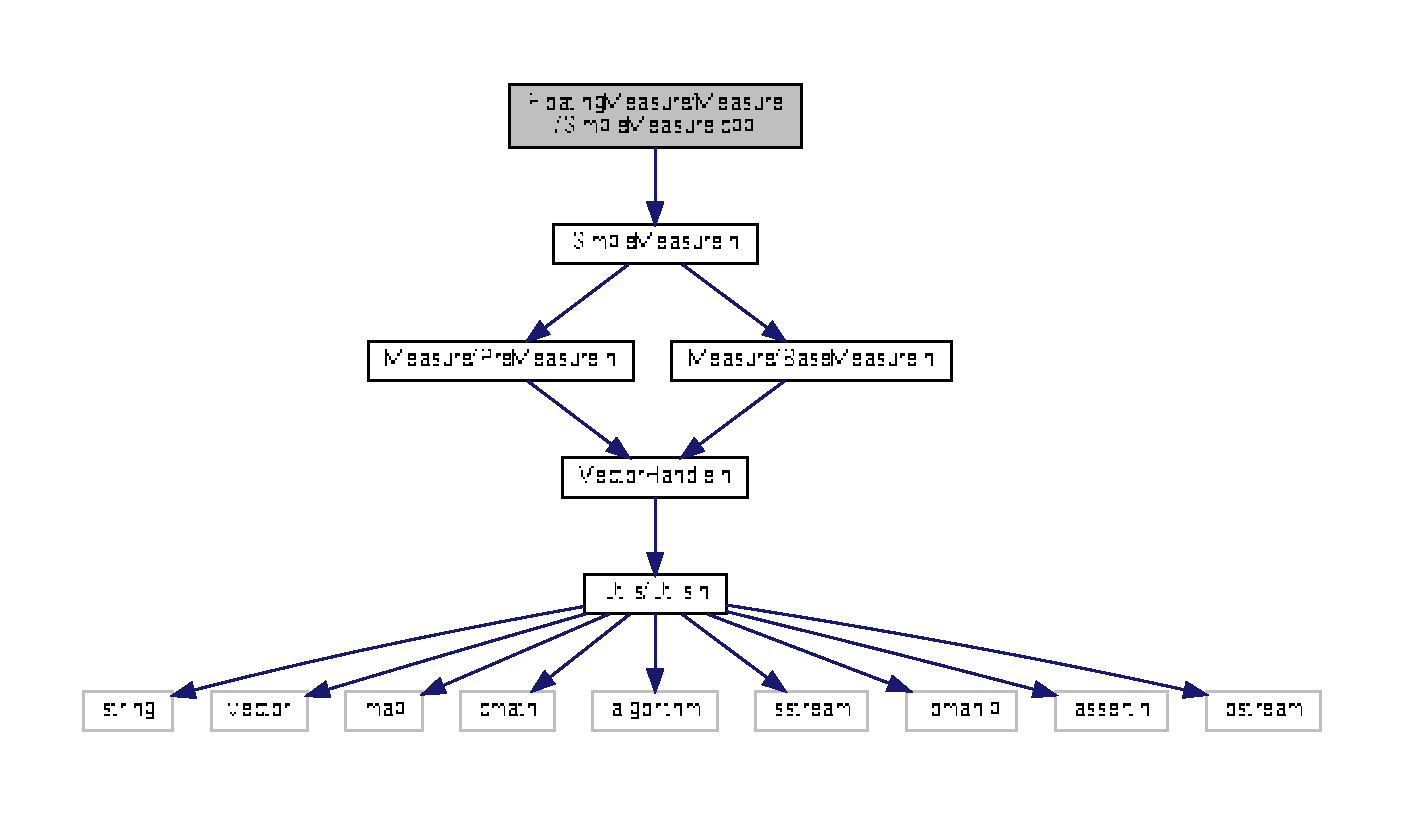
\includegraphics[width=350pt]{d9/d7a/SimpleMeasure_8cpp__incl}
\end{center}
\end{figure}

\hypertarget{SimpleMeasure_8h}{}\section{Floating\+Measure/\+Measure/\+Simple\+Measure.h File Reference}
\label{SimpleMeasure_8h}\index{Floating\+Measure/\+Measure/\+Simple\+Measure.\+h@{Floating\+Measure/\+Measure/\+Simple\+Measure.\+h}}
{\ttfamily \#include $<$Measure/\+Pre\+Measure.\+h$>$}\newline
{\ttfamily \#include $<$Measure/\+Base\+Measure.\+h$>$}\newline
Include dependency graph for Simple\+Measure.\+h\+:\nopagebreak
\begin{figure}[H]
\begin{center}
\leavevmode
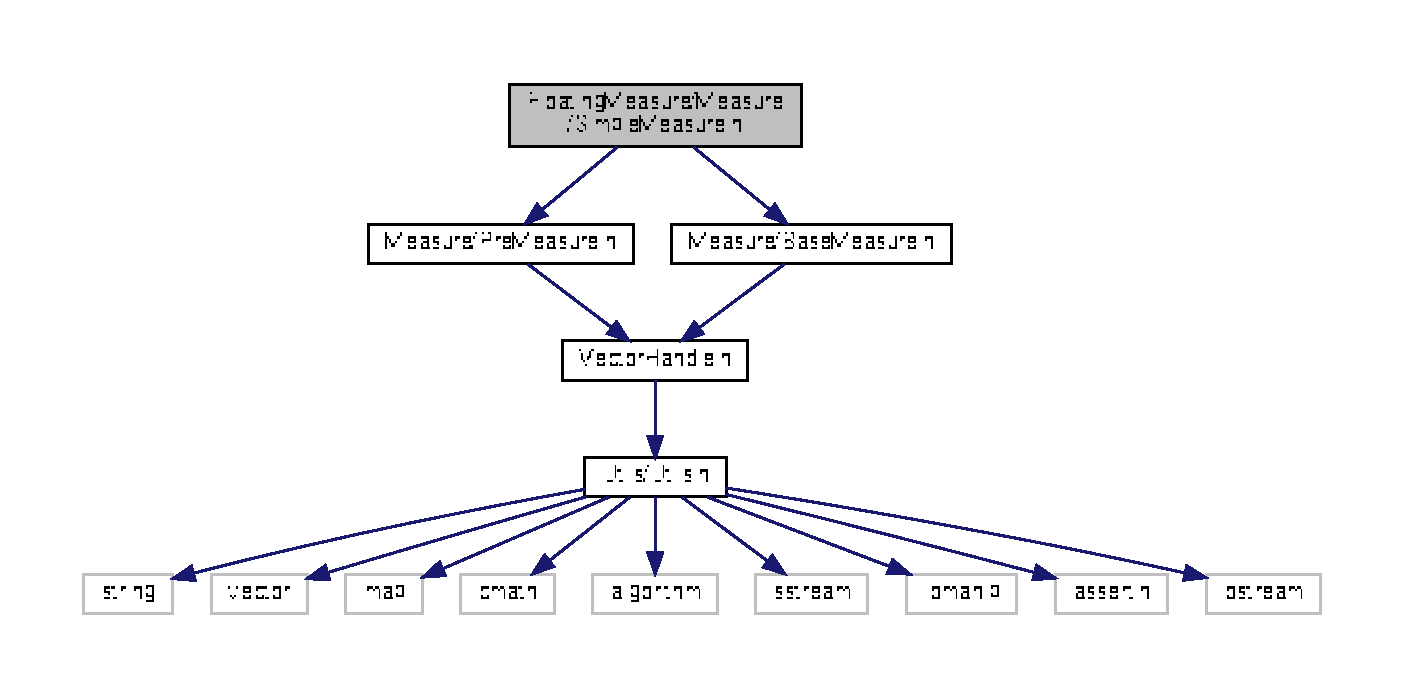
\includegraphics[width=350pt]{dc/d6c/SimpleMeasure_8h__incl}
\end{center}
\end{figure}
This graph shows which files directly or indirectly include this file\+:\nopagebreak
\begin{figure}[H]
\begin{center}
\leavevmode
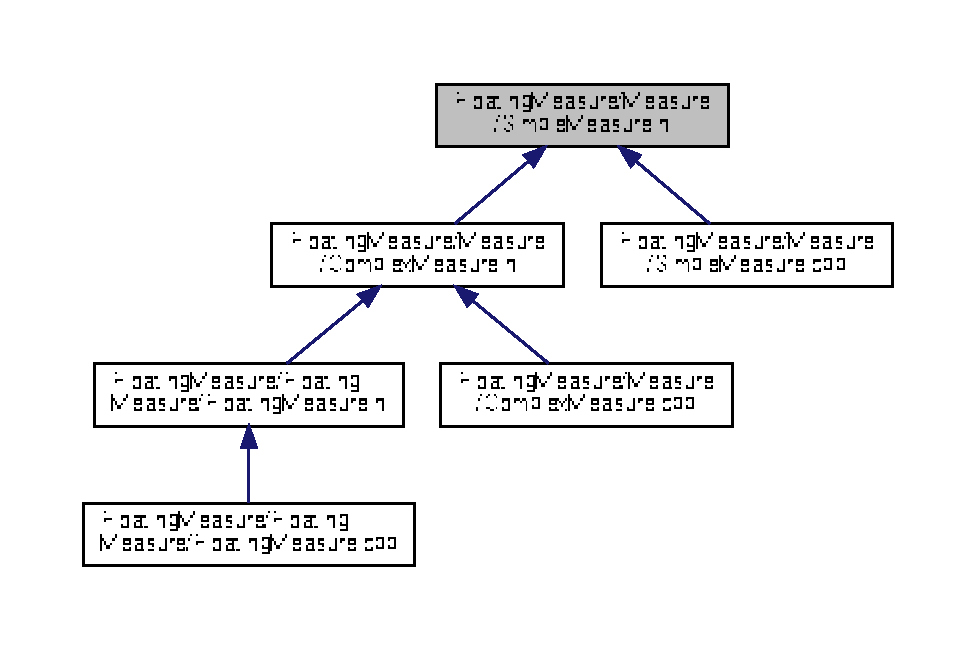
\includegraphics[width=350pt]{d2/d68/SimpleMeasure_8h__dep__incl}
\end{center}
\end{figure}
\subsection*{Classes}
\begin{DoxyCompactItemize}
\item 
class \hyperlink{classCSimpleMeasure}{C\+Simple\+Measure}
\begin{DoxyCompactList}\small\item\em \hyperlink{classCSimpleMeasure}{C\+Simple\+Measure}\+: represents a pre measure combined with a base measure like \char`\"{}m\+V\char`\"{}.~\newline
 This class offers\+: \end{DoxyCompactList}\end{DoxyCompactItemize}

\hypertarget{VectorHandle_8cpp}{}\section{Floating\+Measure/\+Measure/\+Vector\+Handle.cpp File Reference}
\label{VectorHandle_8cpp}\index{Floating\+Measure/\+Measure/\+Vector\+Handle.\+cpp@{Floating\+Measure/\+Measure/\+Vector\+Handle.\+cpp}}
{\ttfamily \#include \char`\"{}Vector\+Handle.\+h\char`\"{}}\newline
Include dependency graph for Vector\+Handle.\+cpp\+:\nopagebreak
\begin{figure}[H]
\begin{center}
\leavevmode
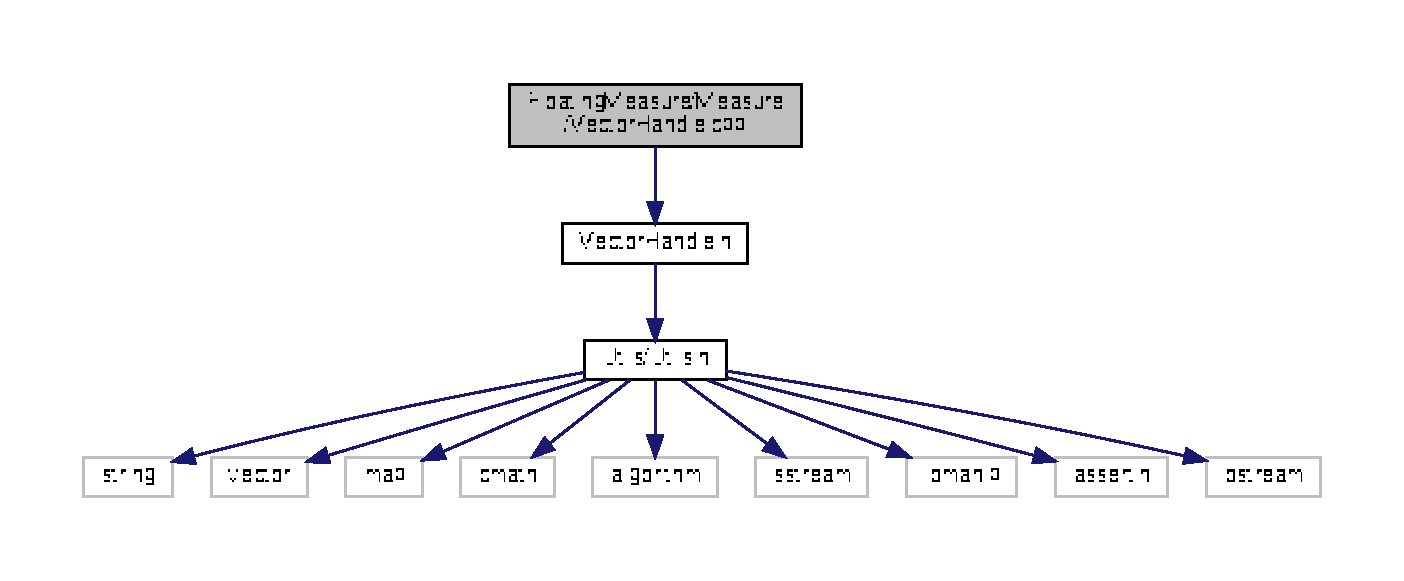
\includegraphics[width=350pt]{d4/de0/VectorHandle_8cpp__incl}
\end{center}
\end{figure}

\hypertarget{VectorHandle_8h}{}\section{Floating\+Measure/\+Measure/\+Vector\+Handle.h File Reference}
\label{VectorHandle_8h}\index{Floating\+Measure/\+Measure/\+Vector\+Handle.\+h@{Floating\+Measure/\+Measure/\+Vector\+Handle.\+h}}
{\ttfamily \#include $<$Utils/\+Utils.\+h$>$}\newline
Include dependency graph for Vector\+Handle.\+h\+:\nopagebreak
\begin{figure}[H]
\begin{center}
\leavevmode
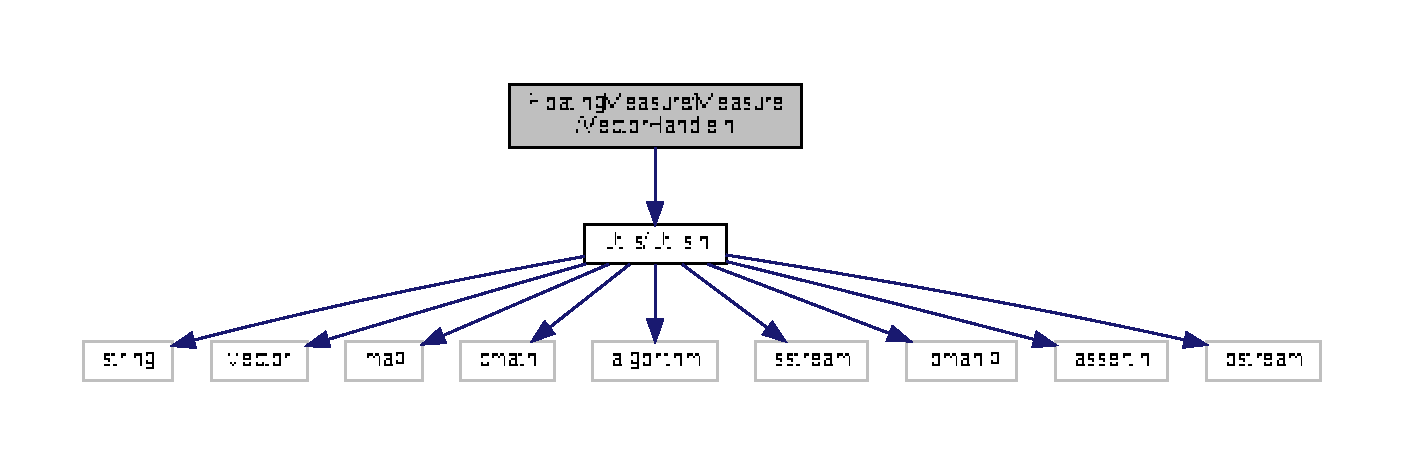
\includegraphics[width=350pt]{df/de7/VectorHandle_8h__incl}
\end{center}
\end{figure}
This graph shows which files directly or indirectly include this file\+:\nopagebreak
\begin{figure}[H]
\begin{center}
\leavevmode
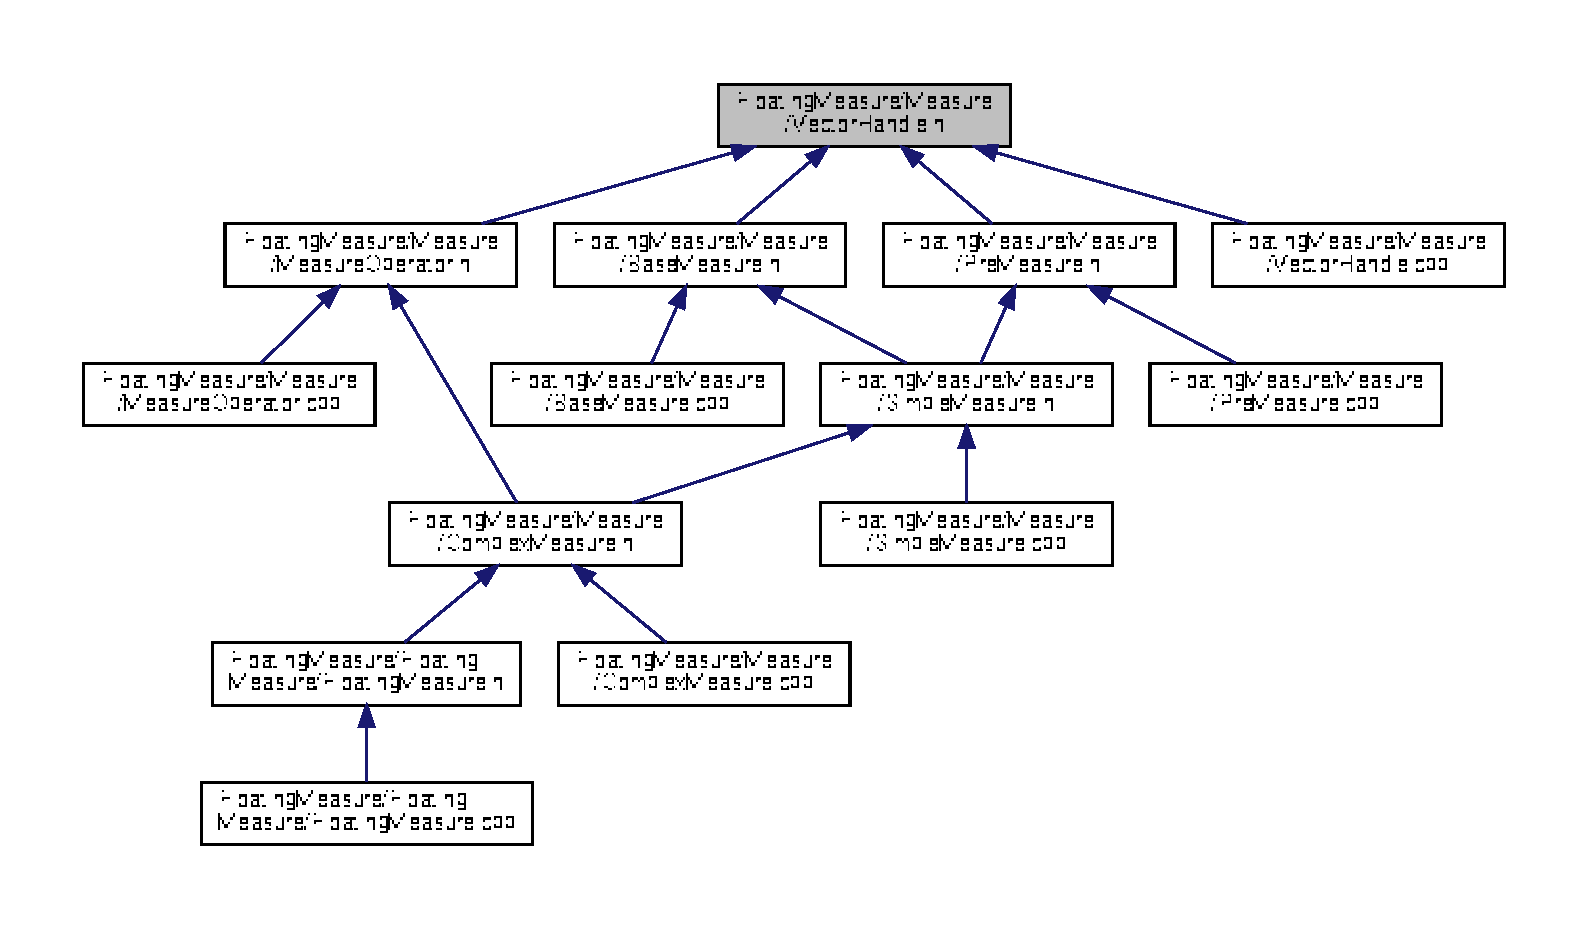
\includegraphics[width=350pt]{da/d92/VectorHandle_8h__dep__incl}
\end{center}
\end{figure}
\subsection*{Classes}
\begin{DoxyCompactItemize}
\item 
class \hyperlink{classCVectorHandle}{C\+Vector\+Handle}
\begin{DoxyCompactList}\small\item\em This class keeps three vectors (two string \+: Short and Long and one double \+: Factor). These vectors are common to classes \hyperlink{classCPreMeasure}{C\+Pre\+Measure} and \hyperlink{classCBaseMeasure}{C\+Base\+Measure} and are therefore packed into this class for vector handling. \end{DoxyCompactList}\end{DoxyCompactItemize}

\hypertarget{Utils_8cpp}{}\section{Floating\+Measure/\+Utils/\+Utils.cpp File Reference}
\label{Utils_8cpp}\index{Floating\+Measure/\+Utils/\+Utils.\+cpp@{Floating\+Measure/\+Utils/\+Utils.\+cpp}}
{\ttfamily \#include $<$Utils/\+Utils.\+h$>$}\newline
Include dependency graph for Utils.\+cpp\+:\nopagebreak
\begin{figure}[H]
\begin{center}
\leavevmode
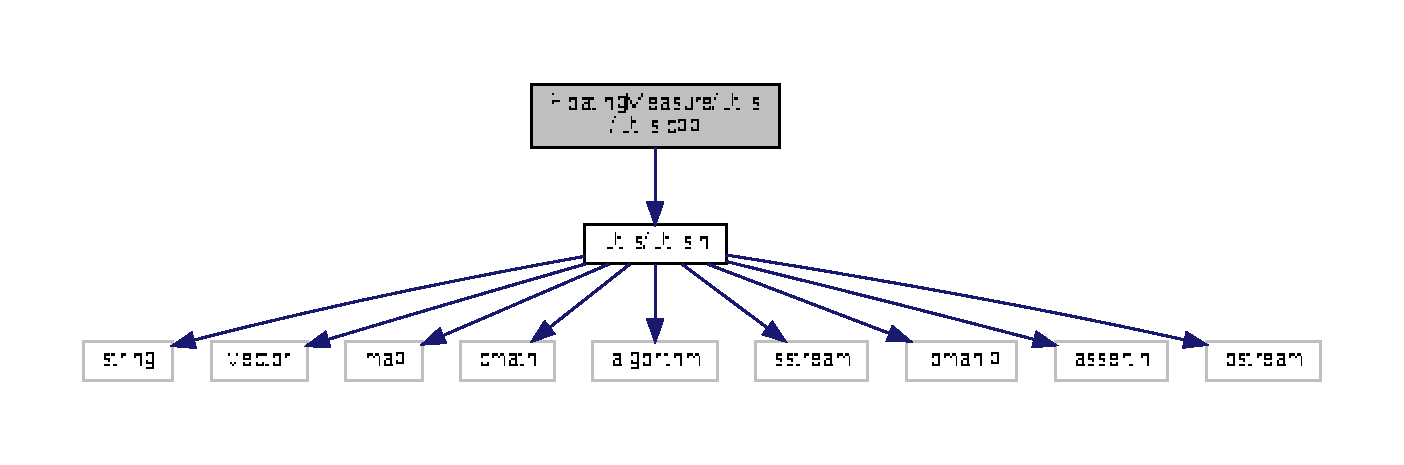
\includegraphics[width=350pt]{de/d88/Utils_8cpp__incl}
\end{center}
\end{figure}
\subsection*{Functions}
\begin{DoxyCompactItemize}
\item 
double \hyperlink{Utils_8cpp_ae9dfc174daaf6261f167ccc069efea93}{Double\+Machine\+Epsilon} (double d\+Value)
\begin{DoxyCompactList}\small\item\em calculates the numerical error for a given double \end{DoxyCompactList}\item 
double \hyperlink{Utils_8cpp_a7dd752b594724a3517f92d86ba0cd39e}{Round2\+Precision} (const double d\+Value, const int n\+Precision)
\begin{DoxyCompactList}\small\item\em cuts double according to precision \end{DoxyCompactList}\item 
string \hyperlink{Utils_8cpp_a78c380ff595f4574b2bb6fa68f15e410}{Bool2\+String} (const bool b\+Bool)
\begin{DoxyCompactList}\small\item\em returns \char`\"{}true\char`\"{} or \char`\"{}false\char`\"{} as string \end{DoxyCompactList}\end{DoxyCompactItemize}


\subsection{Function Documentation}
\mbox{\Hypertarget{Utils_8cpp_a78c380ff595f4574b2bb6fa68f15e410}\label{Utils_8cpp_a78c380ff595f4574b2bb6fa68f15e410}} 
\index{Utils.\+cpp@{Utils.\+cpp}!Bool2\+String@{Bool2\+String}}
\index{Bool2\+String@{Bool2\+String}!Utils.\+cpp@{Utils.\+cpp}}
\subsubsection{\texorpdfstring{Bool2\+String()}{Bool2String()}}
{\footnotesize\ttfamily string Bool2\+String (\begin{DoxyParamCaption}\item[{const bool}]{b\+Bool }\end{DoxyParamCaption})}



returns \char`\"{}true\char`\"{} or \char`\"{}false\char`\"{} as string 


\begin{DoxyParams}{Parameters}
{\em b\+Bool} & bool to convert to string \\
\hline
\end{DoxyParams}
\begin{DoxyReturn}{Returns}
string 
\end{DoxyReturn}


Definition at line 41 of file Utils.\+cpp.

\mbox{\Hypertarget{Utils_8cpp_ae9dfc174daaf6261f167ccc069efea93}\label{Utils_8cpp_ae9dfc174daaf6261f167ccc069efea93}} 
\index{Utils.\+cpp@{Utils.\+cpp}!Double\+Machine\+Epsilon@{Double\+Machine\+Epsilon}}
\index{Double\+Machine\+Epsilon@{Double\+Machine\+Epsilon}!Utils.\+cpp@{Utils.\+cpp}}
\subsubsection{\texorpdfstring{Double\+Machine\+Epsilon()}{DoubleMachineEpsilon()}}
{\footnotesize\ttfamily double Double\+Machine\+Epsilon (\begin{DoxyParamCaption}\item[{double}]{d\+Value }\end{DoxyParamCaption})}



calculates the numerical error for a given double 


\begin{DoxyParams}{Parameters}
{\em d\+Value} & double which error is calculated \\
\hline
\end{DoxyParams}
\begin{DoxyReturn}{Returns}
double 
\end{DoxyReturn}


Definition at line 27 of file Utils.\+cpp.



References dbl\+\_\+64\+::d64, dbl\+\_\+64\+::i64, and s.

\mbox{\Hypertarget{Utils_8cpp_a7dd752b594724a3517f92d86ba0cd39e}\label{Utils_8cpp_a7dd752b594724a3517f92d86ba0cd39e}} 
\index{Utils.\+cpp@{Utils.\+cpp}!Round2\+Precision@{Round2\+Precision}}
\index{Round2\+Precision@{Round2\+Precision}!Utils.\+cpp@{Utils.\+cpp}}
\subsubsection{\texorpdfstring{Round2\+Precision()}{Round2Precision()}}
{\footnotesize\ttfamily double Round2\+Precision (\begin{DoxyParamCaption}\item[{const double}]{d\+Value,  }\item[{const int}]{n\+Precision }\end{DoxyParamCaption})}



cuts double according to precision 


\begin{DoxyItemize}
\item example positive precision\+: value= 100.\+00234, precision = 3 --$>$ 100.\+002
\item example negative precision\+: value 1023404.\+234, precision = -\/2 --$>$ 1023400
\end{DoxyItemize}


\begin{DoxyParams}{Parameters}
{\em d\+Value} & value to be cut \\
\hline
{\em n\+Precision} & the wanted precision \\
\hline
\end{DoxyParams}
\begin{DoxyReturn}{Returns}
double 
\end{DoxyReturn}


Definition at line 35 of file Utils.\+cpp.



References pow().


\hypertarget{Utils_8h}{}\section{Floating\+Measure/\+Utils/\+Utils.h File Reference}
\label{Utils_8h}\index{Floating\+Measure/\+Utils/\+Utils.\+h@{Floating\+Measure/\+Utils/\+Utils.\+h}}
{\ttfamily \#include $<$string$>$}\newline
{\ttfamily \#include $<$vector$>$}\newline
{\ttfamily \#include $<$map$>$}\newline
{\ttfamily \#include $<$cmath$>$}\newline
{\ttfamily \#include $<$algorithm$>$}\newline
{\ttfamily \#include $<$sstream$>$}\newline
{\ttfamily \#include $<$iomanip$>$}\newline
{\ttfamily \#include $<$assert.\+h$>$}\newline
{\ttfamily \#include $<$ostream$>$}\newline
Include dependency graph for Utils.\+h\+:\nopagebreak
\begin{figure}[H]
\begin{center}
\leavevmode
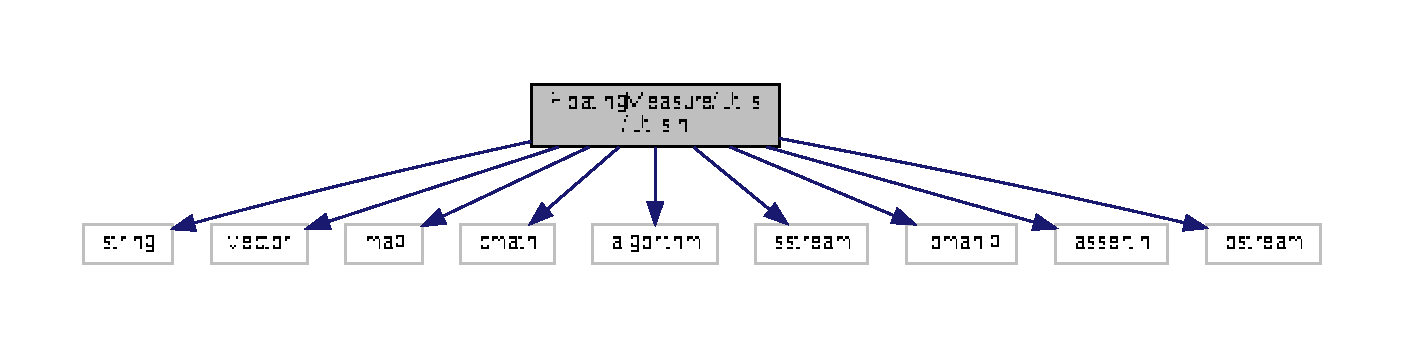
\includegraphics[width=350pt]{db/d5d/Utils_8h__incl}
\end{center}
\end{figure}
This graph shows which files directly or indirectly include this file\+:\nopagebreak
\begin{figure}[H]
\begin{center}
\leavevmode
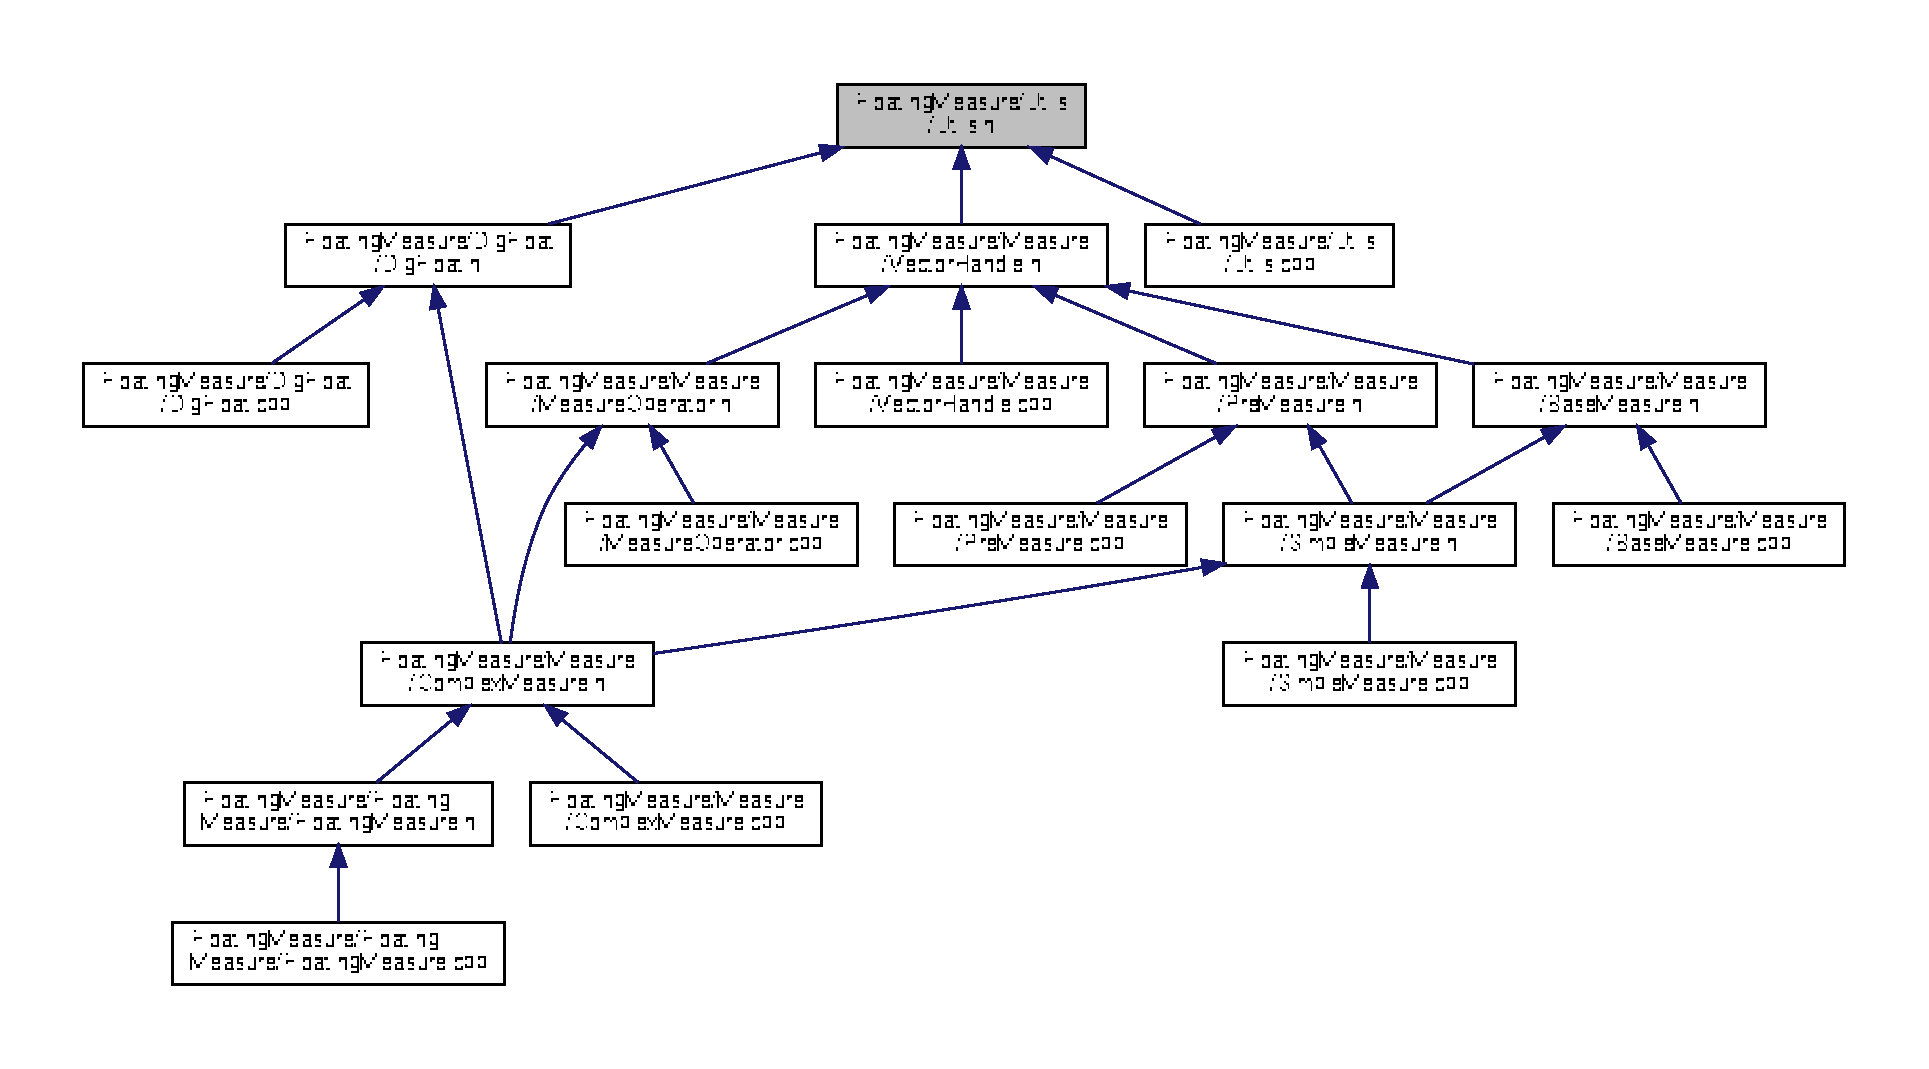
\includegraphics[width=350pt]{d2/dc8/Utils_8h__dep__incl}
\end{center}
\end{figure}
\subsection*{Classes}
\begin{DoxyCompactItemize}
\item 
union \hyperlink{uniondbl__64}{dbl\+\_\+64}
\begin{DoxyCompactList}\small\item\em union for calculation of numerical error of a 64 bit double \end{DoxyCompactList}\item 
class \hyperlink{classCSingleton}{C\+Singleton$<$ Singleton\+Object $>$}
\begin{DoxyCompactList}\small\item\em a Singleton class for a generic Singleton\+Object \end{DoxyCompactList}\end{DoxyCompactItemize}
\subsection*{Macros}
\begin{DoxyCompactItemize}
\item 
\#define \hyperlink{Utils_8h_aa453fe957e6d617b474b45213bf80820}{my\+N\+AN}~nan(\char`\"{}1\char`\"{})
\item 
\#define \hyperlink{Utils_8h_ad65eebfa453cc397aa31c2f1402e7d52}{G\+R\+E\+E\+K\+\_\+\+S\+M\+A\+L\+L\+\_\+\+MU}~\char`\"{}\textbackslash{}u00b5\char`\"{}
\item 
\#define \hyperlink{Utils_8h_a1c7affac54bdfdadac8fd7eb9b062745}{G\+R\+E\+E\+K\+\_\+\+C\+A\+P\+I\+T\+A\+L\+\_\+\+O\+M\+E\+GA}~\char`\"{}\textbackslash{}u03a9\char`\"{}
\item 
\#define \hyperlink{Utils_8h_a8b8d3b6ed23a610665d7e00cb4397680}{U\+N\+K\+N\+O\+W\+N\+\_\+\+S\+H\+O\+RT}~\char`\"{}n.\+a.\char`\"{}
\item 
\#define \hyperlink{Utils_8h_a5c6964ba7806e840a8a24e21191727a3}{U\+N\+K\+N\+O\+W\+N\+\_\+\+L\+O\+NG}~\char`\"{}unknown\char`\"{}
\item 
\#define \hyperlink{Utils_8h_a5a6daae34eeda6d6461f165a02acc3c7}{U\+N\+K\+N\+O\+W\+N\+\_\+\+I\+N\+D\+EX}~-\/1
\item 
\#define \hyperlink{Utils_8h_a0488bc30cccd5b3304bf0936b5af486b}{U\+N\+K\+N\+O\+W\+N\+\_\+\+V\+A\+L\+UE}~\hyperlink{Utils_8h_aa453fe957e6d617b474b45213bf80820}{my\+N\+AN}
\item 
\#define \hyperlink{Utils_8h_a5796288828c990621e30b2669757d916}{I\+N\+V\+A\+L\+I\+D\+\_\+\+E\+X\+P\+O\+N\+E\+NT}~-\/666
\item 
\#define \hyperlink{Utils_8h_a16e1e5ba474fcf3e45ade32acf66c144}{mu}~string(\hyperlink{Utils_8h_ad65eebfa453cc397aa31c2f1402e7d52}{G\+R\+E\+E\+K\+\_\+\+S\+M\+A\+L\+L\+\_\+\+MU})
\item 
\#define \hyperlink{Utils_8h_a400617b5daf9faf9da16780bda2904fd}{Omega}~string(\hyperlink{Utils_8h_a1c7affac54bdfdadac8fd7eb9b062745}{G\+R\+E\+E\+K\+\_\+\+C\+A\+P\+I\+T\+A\+L\+\_\+\+O\+M\+E\+GA})
\item 
\#define \hyperlink{Utils_8h_a57f004e69be4e541c9ef272d1684b9f6}{plmi}~string(\char`\"{}\textbackslash{}u00\+B1\char`\"{})
\end{DoxyCompactItemize}
\subsection*{Functions}
\begin{DoxyCompactItemize}
\item 
double \hyperlink{Utils_8h_ae9dfc174daaf6261f167ccc069efea93}{Double\+Machine\+Epsilon} (double d\+Value)
\begin{DoxyCompactList}\small\item\em calculates the numerical error for a given double \end{DoxyCompactList}\item 
double \hyperlink{Utils_8h_a7dd752b594724a3517f92d86ba0cd39e}{Round2\+Precision} (const double d\+Value, const int n\+Precision)
\begin{DoxyCompactList}\small\item\em cuts double according to precision \end{DoxyCompactList}\item 
string \hyperlink{Utils_8h_a78c380ff595f4574b2bb6fa68f15e410}{Bool2\+String} (const bool b\+Bool)
\begin{DoxyCompactList}\small\item\em returns \char`\"{}true\char`\"{} or \char`\"{}false\char`\"{} as string \end{DoxyCompactList}\item 
{\footnotesize template$<$typename T $>$ }\\int \hyperlink{Utils_8h_aef4e401709c029dcd6fb5ee8a858bdf6}{Find\+Element\+In\+Vector\+Get\+Index} (const T \&Value, const vector$<$ T $>$ \&Vec, int n\+Default\+Index)
\begin{DoxyCompactList}\small\item\em returns the index of an element within a vector \end{DoxyCompactList}\item 
{\footnotesize template$<$typename T $>$ }\\int \hyperlink{Utils_8h_a10f8b0557cff0575f9b545ad76234fcd}{Find\+Element\+In\+Vector\+Get\+Index} (const T \&Value, const vector$<$ T $>$ $\ast$p\+Vec, int n\+Default\+Index)
\begin{DoxyCompactList}\small\item\em returns the index of an element within a vector \end{DoxyCompactList}\item 
{\footnotesize template$<$typename T $>$ }\\const T \& \hyperlink{Utils_8h_a7042c83d0f87835f7fdb87b8d3e1de40}{Get\+Element\+From\+Vector\+By\+Index} (const vector$<$ T $>$ \&Vec, const unsigned int ui\+Index)
\begin{DoxyCompactList}\small\item\em returns the index of an element within a vector \end{DoxyCompactList}\item 
{\footnotesize template$<$typename T $>$ }\\const T \& \hyperlink{Utils_8h_a5dcd880b1990847494e1cfd17b0a0dad}{Get\+Element\+From\+Vector\+By\+Index} (const vector$<$ T $>$ $\ast$p\+Vec, const unsigned int ui\+Index)
\begin{DoxyCompactList}\small\item\em returns the index of an element within a vector \end{DoxyCompactList}\item 
{\footnotesize template$<$typename T $>$ }\\void \hyperlink{Utils_8h_ab3514a1d7de1960b4685ce4eeefce78e}{Secure\+Delete\+Object\+Pointer} (T $\ast$\&pt)
\begin{DoxyCompactList}\small\item\em safely deletes pointers to objects of type T\+:~\newline
 \char`\"{}safely\char`\"{} holds only if unused pointers are initialized with nullptr \end{DoxyCompactList}\item 
{\footnotesize template$<$typename T $>$ }\\void \hyperlink{Utils_8h_aa550c859c03fa28b9b63b7070e53505d}{Secure\+Delete\+Vector\+Pointer} (T $\ast$\&pt)
\begin{DoxyCompactList}\small\item\em safely deletes vectors / arrays of type T \char`\"{}safely\char`\"{} holds only if unused pointers are initialized with nullptr \end{DoxyCompactList}\end{DoxyCompactItemize}


\subsection{Macro Definition Documentation}
\mbox{\Hypertarget{Utils_8h_a1c7affac54bdfdadac8fd7eb9b062745}\label{Utils_8h_a1c7affac54bdfdadac8fd7eb9b062745}} 
\index{Utils.\+h@{Utils.\+h}!G\+R\+E\+E\+K\+\_\+\+C\+A\+P\+I\+T\+A\+L\+\_\+\+O\+M\+E\+GA@{G\+R\+E\+E\+K\+\_\+\+C\+A\+P\+I\+T\+A\+L\+\_\+\+O\+M\+E\+GA}}
\index{G\+R\+E\+E\+K\+\_\+\+C\+A\+P\+I\+T\+A\+L\+\_\+\+O\+M\+E\+GA@{G\+R\+E\+E\+K\+\_\+\+C\+A\+P\+I\+T\+A\+L\+\_\+\+O\+M\+E\+GA}!Utils.\+h@{Utils.\+h}}
\subsubsection{\texorpdfstring{G\+R\+E\+E\+K\+\_\+\+C\+A\+P\+I\+T\+A\+L\+\_\+\+O\+M\+E\+GA}{GREEK\_CAPITAL\_OMEGA}}
{\footnotesize\ttfamily \#define G\+R\+E\+E\+K\+\_\+\+C\+A\+P\+I\+T\+A\+L\+\_\+\+O\+M\+E\+GA~\char`\"{}\textbackslash{}u03a9\char`\"{}}



Definition at line 57 of file Utils.\+h.

\mbox{\Hypertarget{Utils_8h_ad65eebfa453cc397aa31c2f1402e7d52}\label{Utils_8h_ad65eebfa453cc397aa31c2f1402e7d52}} 
\index{Utils.\+h@{Utils.\+h}!G\+R\+E\+E\+K\+\_\+\+S\+M\+A\+L\+L\+\_\+\+MU@{G\+R\+E\+E\+K\+\_\+\+S\+M\+A\+L\+L\+\_\+\+MU}}
\index{G\+R\+E\+E\+K\+\_\+\+S\+M\+A\+L\+L\+\_\+\+MU@{G\+R\+E\+E\+K\+\_\+\+S\+M\+A\+L\+L\+\_\+\+MU}!Utils.\+h@{Utils.\+h}}
\subsubsection{\texorpdfstring{G\+R\+E\+E\+K\+\_\+\+S\+M\+A\+L\+L\+\_\+\+MU}{GREEK\_SMALL\_MU}}
{\footnotesize\ttfamily \#define G\+R\+E\+E\+K\+\_\+\+S\+M\+A\+L\+L\+\_\+\+MU~\char`\"{}\textbackslash{}u00b5\char`\"{}}



Definition at line 56 of file Utils.\+h.

\mbox{\Hypertarget{Utils_8h_a5796288828c990621e30b2669757d916}\label{Utils_8h_a5796288828c990621e30b2669757d916}} 
\index{Utils.\+h@{Utils.\+h}!I\+N\+V\+A\+L\+I\+D\+\_\+\+E\+X\+P\+O\+N\+E\+NT@{I\+N\+V\+A\+L\+I\+D\+\_\+\+E\+X\+P\+O\+N\+E\+NT}}
\index{I\+N\+V\+A\+L\+I\+D\+\_\+\+E\+X\+P\+O\+N\+E\+NT@{I\+N\+V\+A\+L\+I\+D\+\_\+\+E\+X\+P\+O\+N\+E\+NT}!Utils.\+h@{Utils.\+h}}
\subsubsection{\texorpdfstring{I\+N\+V\+A\+L\+I\+D\+\_\+\+E\+X\+P\+O\+N\+E\+NT}{INVALID\_EXPONENT}}
{\footnotesize\ttfamily \#define I\+N\+V\+A\+L\+I\+D\+\_\+\+E\+X\+P\+O\+N\+E\+NT~-\/666}



Definition at line 62 of file Utils.\+h.

\mbox{\Hypertarget{Utils_8h_a16e1e5ba474fcf3e45ade32acf66c144}\label{Utils_8h_a16e1e5ba474fcf3e45ade32acf66c144}} 
\index{Utils.\+h@{Utils.\+h}!mu@{mu}}
\index{mu@{mu}!Utils.\+h@{Utils.\+h}}
\subsubsection{\texorpdfstring{mu}{mu}}
{\footnotesize\ttfamily \#define mu~string(\hyperlink{Utils_8h_ad65eebfa453cc397aa31c2f1402e7d52}{G\+R\+E\+E\+K\+\_\+\+S\+M\+A\+L\+L\+\_\+\+MU})}



Definition at line 70 of file Utils.\+h.

\mbox{\Hypertarget{Utils_8h_aa453fe957e6d617b474b45213bf80820}\label{Utils_8h_aa453fe957e6d617b474b45213bf80820}} 
\index{Utils.\+h@{Utils.\+h}!my\+N\+AN@{my\+N\+AN}}
\index{my\+N\+AN@{my\+N\+AN}!Utils.\+h@{Utils.\+h}}
\subsubsection{\texorpdfstring{my\+N\+AN}{myNAN}}
{\footnotesize\ttfamily \#define my\+N\+AN~nan(\char`\"{}1\char`\"{})}



Definition at line 55 of file Utils.\+h.

\mbox{\Hypertarget{Utils_8h_a400617b5daf9faf9da16780bda2904fd}\label{Utils_8h_a400617b5daf9faf9da16780bda2904fd}} 
\index{Utils.\+h@{Utils.\+h}!Omega@{Omega}}
\index{Omega@{Omega}!Utils.\+h@{Utils.\+h}}
\subsubsection{\texorpdfstring{Omega}{Omega}}
{\footnotesize\ttfamily \#define Omega~string(\hyperlink{Utils_8h_a1c7affac54bdfdadac8fd7eb9b062745}{G\+R\+E\+E\+K\+\_\+\+C\+A\+P\+I\+T\+A\+L\+\_\+\+O\+M\+E\+GA})}



Definition at line 71 of file Utils.\+h.

\mbox{\Hypertarget{Utils_8h_a57f004e69be4e541c9ef272d1684b9f6}\label{Utils_8h_a57f004e69be4e541c9ef272d1684b9f6}} 
\index{Utils.\+h@{Utils.\+h}!plmi@{plmi}}
\index{plmi@{plmi}!Utils.\+h@{Utils.\+h}}
\subsubsection{\texorpdfstring{plmi}{plmi}}
{\footnotesize\ttfamily \#define plmi~string(\char`\"{}\textbackslash{}u00\+B1\char`\"{})}



Definition at line 72 of file Utils.\+h.

\mbox{\Hypertarget{Utils_8h_a5a6daae34eeda6d6461f165a02acc3c7}\label{Utils_8h_a5a6daae34eeda6d6461f165a02acc3c7}} 
\index{Utils.\+h@{Utils.\+h}!U\+N\+K\+N\+O\+W\+N\+\_\+\+I\+N\+D\+EX@{U\+N\+K\+N\+O\+W\+N\+\_\+\+I\+N\+D\+EX}}
\index{U\+N\+K\+N\+O\+W\+N\+\_\+\+I\+N\+D\+EX@{U\+N\+K\+N\+O\+W\+N\+\_\+\+I\+N\+D\+EX}!Utils.\+h@{Utils.\+h}}
\subsubsection{\texorpdfstring{U\+N\+K\+N\+O\+W\+N\+\_\+\+I\+N\+D\+EX}{UNKNOWN\_INDEX}}
{\footnotesize\ttfamily \#define U\+N\+K\+N\+O\+W\+N\+\_\+\+I\+N\+D\+EX~-\/1}



Definition at line 60 of file Utils.\+h.

\mbox{\Hypertarget{Utils_8h_a5c6964ba7806e840a8a24e21191727a3}\label{Utils_8h_a5c6964ba7806e840a8a24e21191727a3}} 
\index{Utils.\+h@{Utils.\+h}!U\+N\+K\+N\+O\+W\+N\+\_\+\+L\+O\+NG@{U\+N\+K\+N\+O\+W\+N\+\_\+\+L\+O\+NG}}
\index{U\+N\+K\+N\+O\+W\+N\+\_\+\+L\+O\+NG@{U\+N\+K\+N\+O\+W\+N\+\_\+\+L\+O\+NG}!Utils.\+h@{Utils.\+h}}
\subsubsection{\texorpdfstring{U\+N\+K\+N\+O\+W\+N\+\_\+\+L\+O\+NG}{UNKNOWN\_LONG}}
{\footnotesize\ttfamily \#define U\+N\+K\+N\+O\+W\+N\+\_\+\+L\+O\+NG~\char`\"{}unknown\char`\"{}}



Definition at line 59 of file Utils.\+h.

\mbox{\Hypertarget{Utils_8h_a8b8d3b6ed23a610665d7e00cb4397680}\label{Utils_8h_a8b8d3b6ed23a610665d7e00cb4397680}} 
\index{Utils.\+h@{Utils.\+h}!U\+N\+K\+N\+O\+W\+N\+\_\+\+S\+H\+O\+RT@{U\+N\+K\+N\+O\+W\+N\+\_\+\+S\+H\+O\+RT}}
\index{U\+N\+K\+N\+O\+W\+N\+\_\+\+S\+H\+O\+RT@{U\+N\+K\+N\+O\+W\+N\+\_\+\+S\+H\+O\+RT}!Utils.\+h@{Utils.\+h}}
\subsubsection{\texorpdfstring{U\+N\+K\+N\+O\+W\+N\+\_\+\+S\+H\+O\+RT}{UNKNOWN\_SHORT}}
{\footnotesize\ttfamily \#define U\+N\+K\+N\+O\+W\+N\+\_\+\+S\+H\+O\+RT~\char`\"{}n.\+a.\char`\"{}}



Definition at line 58 of file Utils.\+h.

\mbox{\Hypertarget{Utils_8h_a0488bc30cccd5b3304bf0936b5af486b}\label{Utils_8h_a0488bc30cccd5b3304bf0936b5af486b}} 
\index{Utils.\+h@{Utils.\+h}!U\+N\+K\+N\+O\+W\+N\+\_\+\+V\+A\+L\+UE@{U\+N\+K\+N\+O\+W\+N\+\_\+\+V\+A\+L\+UE}}
\index{U\+N\+K\+N\+O\+W\+N\+\_\+\+V\+A\+L\+UE@{U\+N\+K\+N\+O\+W\+N\+\_\+\+V\+A\+L\+UE}!Utils.\+h@{Utils.\+h}}
\subsubsection{\texorpdfstring{U\+N\+K\+N\+O\+W\+N\+\_\+\+V\+A\+L\+UE}{UNKNOWN\_VALUE}}
{\footnotesize\ttfamily \#define U\+N\+K\+N\+O\+W\+N\+\_\+\+V\+A\+L\+UE~\hyperlink{Utils_8h_aa453fe957e6d617b474b45213bf80820}{my\+N\+AN}}



Definition at line 61 of file Utils.\+h.



\subsection{Function Documentation}
\mbox{\Hypertarget{Utils_8h_a78c380ff595f4574b2bb6fa68f15e410}\label{Utils_8h_a78c380ff595f4574b2bb6fa68f15e410}} 
\index{Utils.\+h@{Utils.\+h}!Bool2\+String@{Bool2\+String}}
\index{Bool2\+String@{Bool2\+String}!Utils.\+h@{Utils.\+h}}
\subsubsection{\texorpdfstring{Bool2\+String()}{Bool2String()}}
{\footnotesize\ttfamily string Bool2\+String (\begin{DoxyParamCaption}\item[{const bool}]{b\+Bool }\end{DoxyParamCaption})}



returns \char`\"{}true\char`\"{} or \char`\"{}false\char`\"{} as string 


\begin{DoxyParams}{Parameters}
{\em b\+Bool} & bool to convert to string \\
\hline
\end{DoxyParams}
\begin{DoxyReturn}{Returns}
string 
\end{DoxyReturn}


Definition at line 45 of file Utils.\+cpp.

\mbox{\Hypertarget{Utils_8h_ae9dfc174daaf6261f167ccc069efea93}\label{Utils_8h_ae9dfc174daaf6261f167ccc069efea93}} 
\index{Utils.\+h@{Utils.\+h}!Double\+Machine\+Epsilon@{Double\+Machine\+Epsilon}}
\index{Double\+Machine\+Epsilon@{Double\+Machine\+Epsilon}!Utils.\+h@{Utils.\+h}}
\subsubsection{\texorpdfstring{Double\+Machine\+Epsilon()}{DoubleMachineEpsilon()}}
{\footnotesize\ttfamily double Double\+Machine\+Epsilon (\begin{DoxyParamCaption}\item[{double}]{d\+Value }\end{DoxyParamCaption})}



calculates the numerical error for a given double 


\begin{DoxyParams}{Parameters}
{\em d\+Value} & double which error is calculated \\
\hline
\end{DoxyParams}
\begin{DoxyReturn}{Returns}
double
\end{DoxyReturn}
calculates the numerical error for a given double 

Definition at line 31 of file Utils.\+cpp.



References dbl\+\_\+64\+::d64, dbl\+\_\+64\+::i64, and s.

\mbox{\Hypertarget{Utils_8h_aef4e401709c029dcd6fb5ee8a858bdf6}\label{Utils_8h_aef4e401709c029dcd6fb5ee8a858bdf6}} 
\index{Utils.\+h@{Utils.\+h}!Find\+Element\+In\+Vector\+Get\+Index@{Find\+Element\+In\+Vector\+Get\+Index}}
\index{Find\+Element\+In\+Vector\+Get\+Index@{Find\+Element\+In\+Vector\+Get\+Index}!Utils.\+h@{Utils.\+h}}
\subsubsection{\texorpdfstring{Find\+Element\+In\+Vector\+Get\+Index()}{FindElementInVectorGetIndex()}\hspace{0.1cm}{\footnotesize\ttfamily [1/2]}}
{\footnotesize\ttfamily template$<$typename T $>$ \\
int Find\+Element\+In\+Vector\+Get\+Index (\begin{DoxyParamCaption}\item[{const T \&}]{Value,  }\item[{const vector$<$ T $>$ \&}]{Vec,  }\item[{int}]{n\+Default\+Index }\end{DoxyParamCaption})}



returns the index of an element within a vector 


\begin{DoxyTemplParams}{Template Parameters}
{\em T} & template type \\
\hline
\end{DoxyTemplParams}

\begin{DoxyParams}{Parameters}
{\em Value} & value to find in the vector \\
\hline
{\em Vec} & the vector where the element will be searched \\
\hline
{\em n\+Default\+Index} & the index returned in case the element is not found in the vector \\
\hline
\end{DoxyParams}
\begin{DoxyReturn}{Returns}
int 
\end{DoxyReturn}


Definition at line 211 of file Utils.\+h.

\mbox{\Hypertarget{Utils_8h_a10f8b0557cff0575f9b545ad76234fcd}\label{Utils_8h_a10f8b0557cff0575f9b545ad76234fcd}} 
\index{Utils.\+h@{Utils.\+h}!Find\+Element\+In\+Vector\+Get\+Index@{Find\+Element\+In\+Vector\+Get\+Index}}
\index{Find\+Element\+In\+Vector\+Get\+Index@{Find\+Element\+In\+Vector\+Get\+Index}!Utils.\+h@{Utils.\+h}}
\subsubsection{\texorpdfstring{Find\+Element\+In\+Vector\+Get\+Index()}{FindElementInVectorGetIndex()}\hspace{0.1cm}{\footnotesize\ttfamily [2/2]}}
{\footnotesize\ttfamily template$<$typename T $>$ \\
int Find\+Element\+In\+Vector\+Get\+Index (\begin{DoxyParamCaption}\item[{const T \&}]{Value,  }\item[{const vector$<$ T $>$ $\ast$}]{p\+Vec,  }\item[{int}]{n\+Default\+Index }\end{DoxyParamCaption})}



returns the index of an element within a vector 


\begin{DoxyTemplParams}{Template Parameters}
{\em T} & template type \\
\hline
\end{DoxyTemplParams}

\begin{DoxyParams}{Parameters}
{\em Value} & value to find in the vector \\
\hline
{\em p\+Vec} & the pointer of the vector where the element will be searched \\
\hline
{\em n\+Default\+Index} & the index returned in case the element is not found in the vector \\
\hline
\end{DoxyParams}
\begin{DoxyReturn}{Returns}
int 
\end{DoxyReturn}


Definition at line 236 of file Utils.\+h.



References Find\+Element\+In\+Vector\+Get\+Index().

\mbox{\Hypertarget{Utils_8h_a7042c83d0f87835f7fdb87b8d3e1de40}\label{Utils_8h_a7042c83d0f87835f7fdb87b8d3e1de40}} 
\index{Utils.\+h@{Utils.\+h}!Get\+Element\+From\+Vector\+By\+Index@{Get\+Element\+From\+Vector\+By\+Index}}
\index{Get\+Element\+From\+Vector\+By\+Index@{Get\+Element\+From\+Vector\+By\+Index}!Utils.\+h@{Utils.\+h}}
\subsubsection{\texorpdfstring{Get\+Element\+From\+Vector\+By\+Index()}{GetElementFromVectorByIndex()}\hspace{0.1cm}{\footnotesize\ttfamily [1/2]}}
{\footnotesize\ttfamily template$<$typename T $>$ \\
const T\& Get\+Element\+From\+Vector\+By\+Index (\begin{DoxyParamCaption}\item[{const vector$<$ T $>$ \&}]{Vec,  }\item[{const unsigned int}]{ui\+Index }\end{DoxyParamCaption})}



returns the index of an element within a vector 


\begin{DoxyTemplParams}{Template Parameters}
{\em T} & template type \\
\hline
\end{DoxyTemplParams}

\begin{DoxyParams}{Parameters}
{\em Vec} & the vector where the element will be searched \\
\hline
{\em ui\+Index} & the index of the value returned, in case it exceeds the vector size, the last element of the vector is returned \\
\hline
\end{DoxyParams}
\begin{DoxyReturn}{Returns}
int 
\end{DoxyReturn}


Definition at line 251 of file Utils.\+h.

\mbox{\Hypertarget{Utils_8h_a5dcd880b1990847494e1cfd17b0a0dad}\label{Utils_8h_a5dcd880b1990847494e1cfd17b0a0dad}} 
\index{Utils.\+h@{Utils.\+h}!Get\+Element\+From\+Vector\+By\+Index@{Get\+Element\+From\+Vector\+By\+Index}}
\index{Get\+Element\+From\+Vector\+By\+Index@{Get\+Element\+From\+Vector\+By\+Index}!Utils.\+h@{Utils.\+h}}
\subsubsection{\texorpdfstring{Get\+Element\+From\+Vector\+By\+Index()}{GetElementFromVectorByIndex()}\hspace{0.1cm}{\footnotesize\ttfamily [2/2]}}
{\footnotesize\ttfamily template$<$typename T $>$ \\
const T\& Get\+Element\+From\+Vector\+By\+Index (\begin{DoxyParamCaption}\item[{const vector$<$ T $>$ $\ast$}]{p\+Vec,  }\item[{const unsigned int}]{ui\+Index }\end{DoxyParamCaption})}



returns the index of an element within a vector 


\begin{DoxyTemplParams}{Template Parameters}
{\em T} & template type \\
\hline
\end{DoxyTemplParams}

\begin{DoxyParams}{Parameters}
{\em p\+Vec} & the pointer of the vector where the element will be searched \\
\hline
{\em ui\+Index} & the index of the value returned, in case it exceeds the vector size, the last element of the vector is returned \\
\hline
\end{DoxyParams}
\begin{DoxyReturn}{Returns}
int 
\end{DoxyReturn}


Definition at line 267 of file Utils.\+h.



References Get\+Element\+From\+Vector\+By\+Index().

\mbox{\Hypertarget{Utils_8h_a7dd752b594724a3517f92d86ba0cd39e}\label{Utils_8h_a7dd752b594724a3517f92d86ba0cd39e}} 
\index{Utils.\+h@{Utils.\+h}!Round2\+Precision@{Round2\+Precision}}
\index{Round2\+Precision@{Round2\+Precision}!Utils.\+h@{Utils.\+h}}
\subsubsection{\texorpdfstring{Round2\+Precision()}{Round2Precision()}}
{\footnotesize\ttfamily double Round2\+Precision (\begin{DoxyParamCaption}\item[{const double}]{d\+Value,  }\item[{const int}]{n\+Precision }\end{DoxyParamCaption})}



cuts double according to precision 


\begin{DoxyItemize}
\item example positive precision\+: value= 100.\+00234, precision = 3 --$>$ 100.\+002
\item example negative precision\+: value 1023404.\+234, precision = -\/2 --$>$ 1023400
\end{DoxyItemize}


\begin{DoxyParams}{Parameters}
{\em d\+Value} & value to be cut \\
\hline
{\em n\+Precision} & the wanted precision \\
\hline
\end{DoxyParams}
\begin{DoxyReturn}{Returns}
double 
\end{DoxyReturn}


Definition at line 39 of file Utils.\+cpp.



References pow().

\mbox{\Hypertarget{Utils_8h_ab3514a1d7de1960b4685ce4eeefce78e}\label{Utils_8h_ab3514a1d7de1960b4685ce4eeefce78e}} 
\index{Utils.\+h@{Utils.\+h}!Secure\+Delete\+Object\+Pointer@{Secure\+Delete\+Object\+Pointer}}
\index{Secure\+Delete\+Object\+Pointer@{Secure\+Delete\+Object\+Pointer}!Utils.\+h@{Utils.\+h}}
\subsubsection{\texorpdfstring{Secure\+Delete\+Object\+Pointer()}{SecureDeleteObjectPointer()}}
{\footnotesize\ttfamily template$<$typename T $>$ \\
void Secure\+Delete\+Object\+Pointer (\begin{DoxyParamCaption}\item[{T $\ast$\&}]{pt }\end{DoxyParamCaption})}



safely deletes pointers to objects of type T\+:~\newline
 \char`\"{}safely\char`\"{} holds only if unused pointers are initialized with nullptr 


\begin{DoxyTemplParams}{Template Parameters}
{\em T\+:object} & Type \\
\hline
\end{DoxyTemplParams}

\begin{DoxyParams}{Parameters}
{\em pt} & pointer \\
\hline
\end{DoxyParams}


Definition at line 280 of file Utils.\+h.

\mbox{\Hypertarget{Utils_8h_aa550c859c03fa28b9b63b7070e53505d}\label{Utils_8h_aa550c859c03fa28b9b63b7070e53505d}} 
\index{Utils.\+h@{Utils.\+h}!Secure\+Delete\+Vector\+Pointer@{Secure\+Delete\+Vector\+Pointer}}
\index{Secure\+Delete\+Vector\+Pointer@{Secure\+Delete\+Vector\+Pointer}!Utils.\+h@{Utils.\+h}}
\subsubsection{\texorpdfstring{Secure\+Delete\+Vector\+Pointer()}{SecureDeleteVectorPointer()}}
{\footnotesize\ttfamily template$<$typename T $>$ \\
void Secure\+Delete\+Vector\+Pointer (\begin{DoxyParamCaption}\item[{T $\ast$\&}]{pt }\end{DoxyParamCaption})}



safely deletes vectors / arrays of type T \char`\"{}safely\char`\"{} holds only if unused pointers are initialized with nullptr 


\begin{DoxyTemplParams}{Template Parameters}
{\em T} & object type \\
\hline
\end{DoxyTemplParams}

\begin{DoxyParams}{Parameters}
{\em pt} & pointer of vector / array \\
\hline
\end{DoxyParams}


Definition at line 295 of file Utils.\+h.


%--- End generated contents ---

% Index
\backmatter
\newpage
\phantomsection
\clearemptydoublepage
\addcontentsline{toc}{chapter}{Index}
\printindex

\end{document}
